\section{Case Study: Heart Failure}

\subsection{Time-series Clustering}

\begin{figure}[htb]
    \centering
    % \includegraphics[width=\textwidth]{results/tsc_hf_dor_sens_spec_dist.png}
    %% Creator: Matplotlib, PGF backend
%%
%% To include the figure in your LaTeX document, write
%%   \input{<filename>.pgf}
%%
%% Make sure the required packages are loaded in your preamble
%%   \usepackage{pgf}
%%
%% Figures using additional raster images can only be included by \input if
%% they are in the same directory as the main LaTeX file. For loading figures
%% from other directories you can use the `import` package
%%   \usepackage{import}
%% and then include the figures with
%%   \import{<path to file>}{<filename>.pgf}
%%
%% Matplotlib used the following preamble
%%
\begingroup%
\makeatletter%
\begin{pgfpicture}%
\pgfpathrectangle{\pgfpointorigin}{\pgfqpoint{6.364000in}{2.540000in}}%
\pgfusepath{use as bounding box, clip}%
\begin{pgfscope}%
\pgfsetbuttcap%
\pgfsetmiterjoin%
\definecolor{currentfill}{rgb}{1.000000,1.000000,1.000000}%
\pgfsetfillcolor{currentfill}%
\pgfsetlinewidth{0.000000pt}%
\definecolor{currentstroke}{rgb}{1.000000,1.000000,1.000000}%
\pgfsetstrokecolor{currentstroke}%
\pgfsetdash{}{0pt}%
\pgfpathmoveto{\pgfqpoint{0.000000in}{0.000000in}}%
\pgfpathlineto{\pgfqpoint{6.364000in}{0.000000in}}%
\pgfpathlineto{\pgfqpoint{6.364000in}{2.540000in}}%
\pgfpathlineto{\pgfqpoint{0.000000in}{2.540000in}}%
\pgfpathclose%
\pgfusepath{fill}%
\end{pgfscope}%
\begin{pgfscope}%
\pgfsetbuttcap%
\pgfsetmiterjoin%
\definecolor{currentfill}{rgb}{0.917647,0.917647,0.949020}%
\pgfsetfillcolor{currentfill}%
\pgfsetlinewidth{0.000000pt}%
\definecolor{currentstroke}{rgb}{0.000000,0.000000,0.000000}%
\pgfsetstrokecolor{currentstroke}%
\pgfsetstrokeopacity{0.000000}%
\pgfsetdash{}{0pt}%
\pgfpathmoveto{\pgfqpoint{0.650810in}{0.557870in}}%
\pgfpathlineto{\pgfqpoint{3.096898in}{0.557870in}}%
\pgfpathlineto{\pgfqpoint{3.096898in}{2.242604in}}%
\pgfpathlineto{\pgfqpoint{0.650810in}{2.242604in}}%
\pgfpathclose%
\pgfusepath{fill}%
\end{pgfscope}%
\begin{pgfscope}%
\pgfpathrectangle{\pgfqpoint{0.650810in}{0.557870in}}{\pgfqpoint{2.446088in}{1.684734in}}%
\pgfusepath{clip}%
\pgfsetroundcap%
\pgfsetroundjoin%
\pgfsetlinewidth{1.003750pt}%
\definecolor{currentstroke}{rgb}{1.000000,1.000000,1.000000}%
\pgfsetstrokecolor{currentstroke}%
\pgfsetdash{}{0pt}%
\pgfpathmoveto{\pgfqpoint{0.761996in}{0.557870in}}%
\pgfpathlineto{\pgfqpoint{0.761996in}{2.242604in}}%
\pgfusepath{stroke}%
\end{pgfscope}%
\begin{pgfscope}%
\definecolor{textcolor}{rgb}{0.150000,0.150000,0.150000}%
\pgfsetstrokecolor{textcolor}%
\pgfsetfillcolor{textcolor}%
\pgftext[x=0.761996in,y=0.425926in,,top]{\color{textcolor}\sffamily\fontsize{11.000000}{13.200000}\selectfont \(\displaystyle 0\)}%
\end{pgfscope}%
\begin{pgfscope}%
\pgfpathrectangle{\pgfqpoint{0.650810in}{0.557870in}}{\pgfqpoint{2.446088in}{1.684734in}}%
\pgfusepath{clip}%
\pgfsetroundcap%
\pgfsetroundjoin%
\pgfsetlinewidth{1.003750pt}%
\definecolor{currentstroke}{rgb}{1.000000,1.000000,1.000000}%
\pgfsetstrokecolor{currentstroke}%
\pgfsetdash{}{0pt}%
\pgfpathmoveto{\pgfqpoint{1.710787in}{0.557870in}}%
\pgfpathlineto{\pgfqpoint{1.710787in}{2.242604in}}%
\pgfusepath{stroke}%
\end{pgfscope}%
\begin{pgfscope}%
\definecolor{textcolor}{rgb}{0.150000,0.150000,0.150000}%
\pgfsetstrokecolor{textcolor}%
\pgfsetfillcolor{textcolor}%
\pgftext[x=1.710787in,y=0.425926in,,top]{\color{textcolor}\sffamily\fontsize{11.000000}{13.200000}\selectfont \(\displaystyle 5\)}%
\end{pgfscope}%
\begin{pgfscope}%
\pgfpathrectangle{\pgfqpoint{0.650810in}{0.557870in}}{\pgfqpoint{2.446088in}{1.684734in}}%
\pgfusepath{clip}%
\pgfsetroundcap%
\pgfsetroundjoin%
\pgfsetlinewidth{1.003750pt}%
\definecolor{currentstroke}{rgb}{1.000000,1.000000,1.000000}%
\pgfsetstrokecolor{currentstroke}%
\pgfsetdash{}{0pt}%
\pgfpathmoveto{\pgfqpoint{2.659578in}{0.557870in}}%
\pgfpathlineto{\pgfqpoint{2.659578in}{2.242604in}}%
\pgfusepath{stroke}%
\end{pgfscope}%
\begin{pgfscope}%
\definecolor{textcolor}{rgb}{0.150000,0.150000,0.150000}%
\pgfsetstrokecolor{textcolor}%
\pgfsetfillcolor{textcolor}%
\pgftext[x=2.659578in,y=0.425926in,,top]{\color{textcolor}\sffamily\fontsize{11.000000}{13.200000}\selectfont \(\displaystyle 10\)}%
\end{pgfscope}%
\begin{pgfscope}%
\definecolor{textcolor}{rgb}{0.150000,0.150000,0.150000}%
\pgfsetstrokecolor{textcolor}%
\pgfsetfillcolor{textcolor}%
\pgftext[x=1.873854in,y=0.235185in,,top]{\color{textcolor}\sffamily\fontsize{11.000000}{13.200000}\selectfont DOR}%
\end{pgfscope}%
\begin{pgfscope}%
\pgfpathrectangle{\pgfqpoint{0.650810in}{0.557870in}}{\pgfqpoint{2.446088in}{1.684734in}}%
\pgfusepath{clip}%
\pgfsetroundcap%
\pgfsetroundjoin%
\pgfsetlinewidth{1.003750pt}%
\definecolor{currentstroke}{rgb}{1.000000,1.000000,1.000000}%
\pgfsetstrokecolor{currentstroke}%
\pgfsetdash{}{0pt}%
\pgfpathmoveto{\pgfqpoint{0.650810in}{0.557870in}}%
\pgfpathlineto{\pgfqpoint{3.096898in}{0.557870in}}%
\pgfusepath{stroke}%
\end{pgfscope}%
\begin{pgfscope}%
\definecolor{textcolor}{rgb}{0.150000,0.150000,0.150000}%
\pgfsetstrokecolor{textcolor}%
\pgfsetfillcolor{textcolor}%
\pgftext[x=0.442824in,y=0.505064in,left,base]{\color{textcolor}\sffamily\fontsize{11.000000}{13.200000}\selectfont \(\displaystyle 0\)}%
\end{pgfscope}%
\begin{pgfscope}%
\pgfpathrectangle{\pgfqpoint{0.650810in}{0.557870in}}{\pgfqpoint{2.446088in}{1.684734in}}%
\pgfusepath{clip}%
\pgfsetroundcap%
\pgfsetroundjoin%
\pgfsetlinewidth{1.003750pt}%
\definecolor{currentstroke}{rgb}{1.000000,1.000000,1.000000}%
\pgfsetstrokecolor{currentstroke}%
\pgfsetdash{}{0pt}%
\pgfpathmoveto{\pgfqpoint{0.650810in}{1.135032in}}%
\pgfpathlineto{\pgfqpoint{3.096898in}{1.135032in}}%
\pgfusepath{stroke}%
\end{pgfscope}%
\begin{pgfscope}%
\definecolor{textcolor}{rgb}{0.150000,0.150000,0.150000}%
\pgfsetstrokecolor{textcolor}%
\pgfsetfillcolor{textcolor}%
\pgftext[x=0.366783in,y=1.082225in,left,base]{\color{textcolor}\sffamily\fontsize{11.000000}{13.200000}\selectfont \(\displaystyle 50\)}%
\end{pgfscope}%
\begin{pgfscope}%
\pgfpathrectangle{\pgfqpoint{0.650810in}{0.557870in}}{\pgfqpoint{2.446088in}{1.684734in}}%
\pgfusepath{clip}%
\pgfsetroundcap%
\pgfsetroundjoin%
\pgfsetlinewidth{1.003750pt}%
\definecolor{currentstroke}{rgb}{1.000000,1.000000,1.000000}%
\pgfsetstrokecolor{currentstroke}%
\pgfsetdash{}{0pt}%
\pgfpathmoveto{\pgfqpoint{0.650810in}{1.712193in}}%
\pgfpathlineto{\pgfqpoint{3.096898in}{1.712193in}}%
\pgfusepath{stroke}%
\end{pgfscope}%
\begin{pgfscope}%
\definecolor{textcolor}{rgb}{0.150000,0.150000,0.150000}%
\pgfsetstrokecolor{textcolor}%
\pgfsetfillcolor{textcolor}%
\pgftext[x=0.290741in,y=1.659386in,left,base]{\color{textcolor}\sffamily\fontsize{11.000000}{13.200000}\selectfont \(\displaystyle 100\)}%
\end{pgfscope}%
\begin{pgfscope}%
\definecolor{textcolor}{rgb}{0.150000,0.150000,0.150000}%
\pgfsetstrokecolor{textcolor}%
\pgfsetfillcolor{textcolor}%
\pgftext[x=0.235185in,y=1.400237in,,bottom,rotate=90.000000]{\color{textcolor}\sffamily\fontsize{11.000000}{13.200000}\selectfont Occurance}%
\end{pgfscope}%
\begin{pgfscope}%
\pgfpathrectangle{\pgfqpoint{0.650810in}{0.557870in}}{\pgfqpoint{2.446088in}{1.684734in}}%
\pgfusepath{clip}%
\pgfsetbuttcap%
\pgfsetmiterjoin%
\definecolor{currentfill}{rgb}{0.298039,0.447059,0.690196}%
\pgfsetfillcolor{currentfill}%
\pgfsetfillopacity{0.400000}%
\pgfsetlinewidth{1.003750pt}%
\definecolor{currentstroke}{rgb}{1.000000,1.000000,1.000000}%
\pgfsetstrokecolor{currentstroke}%
\pgfsetstrokeopacity{0.400000}%
\pgfsetdash{}{0pt}%
\pgfpathmoveto{\pgfqpoint{0.761996in}{0.557870in}}%
\pgfpathlineto{\pgfqpoint{0.984368in}{0.557870in}}%
\pgfpathlineto{\pgfqpoint{0.984368in}{2.162379in}}%
\pgfpathlineto{\pgfqpoint{0.761996in}{2.162379in}}%
\pgfpathclose%
\pgfusepath{stroke,fill}%
\end{pgfscope}%
\begin{pgfscope}%
\pgfpathrectangle{\pgfqpoint{0.650810in}{0.557870in}}{\pgfqpoint{2.446088in}{1.684734in}}%
\pgfusepath{clip}%
\pgfsetbuttcap%
\pgfsetmiterjoin%
\definecolor{currentfill}{rgb}{0.298039,0.447059,0.690196}%
\pgfsetfillcolor{currentfill}%
\pgfsetfillopacity{0.400000}%
\pgfsetlinewidth{1.003750pt}%
\definecolor{currentstroke}{rgb}{1.000000,1.000000,1.000000}%
\pgfsetstrokecolor{currentstroke}%
\pgfsetstrokeopacity{0.400000}%
\pgfsetdash{}{0pt}%
\pgfpathmoveto{\pgfqpoint{0.984368in}{0.557870in}}%
\pgfpathlineto{\pgfqpoint{1.206739in}{0.557870in}}%
\pgfpathlineto{\pgfqpoint{1.206739in}{0.996513in}}%
\pgfpathlineto{\pgfqpoint{0.984368in}{0.996513in}}%
\pgfpathclose%
\pgfusepath{stroke,fill}%
\end{pgfscope}%
\begin{pgfscope}%
\pgfpathrectangle{\pgfqpoint{0.650810in}{0.557870in}}{\pgfqpoint{2.446088in}{1.684734in}}%
\pgfusepath{clip}%
\pgfsetbuttcap%
\pgfsetmiterjoin%
\definecolor{currentfill}{rgb}{0.298039,0.447059,0.690196}%
\pgfsetfillcolor{currentfill}%
\pgfsetfillopacity{0.400000}%
\pgfsetlinewidth{1.003750pt}%
\definecolor{currentstroke}{rgb}{1.000000,1.000000,1.000000}%
\pgfsetstrokecolor{currentstroke}%
\pgfsetstrokeopacity{0.400000}%
\pgfsetdash{}{0pt}%
\pgfpathmoveto{\pgfqpoint{1.206739in}{0.557870in}}%
\pgfpathlineto{\pgfqpoint{1.429111in}{0.557870in}}%
\pgfpathlineto{\pgfqpoint{1.429111in}{0.604043in}}%
\pgfpathlineto{\pgfqpoint{1.206739in}{0.604043in}}%
\pgfpathclose%
\pgfusepath{stroke,fill}%
\end{pgfscope}%
\begin{pgfscope}%
\pgfpathrectangle{\pgfqpoint{0.650810in}{0.557870in}}{\pgfqpoint{2.446088in}{1.684734in}}%
\pgfusepath{clip}%
\pgfsetbuttcap%
\pgfsetmiterjoin%
\definecolor{currentfill}{rgb}{0.298039,0.447059,0.690196}%
\pgfsetfillcolor{currentfill}%
\pgfsetfillopacity{0.400000}%
\pgfsetlinewidth{1.003750pt}%
\definecolor{currentstroke}{rgb}{1.000000,1.000000,1.000000}%
\pgfsetstrokecolor{currentstroke}%
\pgfsetstrokeopacity{0.400000}%
\pgfsetdash{}{0pt}%
\pgfpathmoveto{\pgfqpoint{1.429111in}{0.557870in}}%
\pgfpathlineto{\pgfqpoint{1.651483in}{0.557870in}}%
\pgfpathlineto{\pgfqpoint{1.651483in}{0.927254in}}%
\pgfpathlineto{\pgfqpoint{1.429111in}{0.927254in}}%
\pgfpathclose%
\pgfusepath{stroke,fill}%
\end{pgfscope}%
\begin{pgfscope}%
\pgfpathrectangle{\pgfqpoint{0.650810in}{0.557870in}}{\pgfqpoint{2.446088in}{1.684734in}}%
\pgfusepath{clip}%
\pgfsetbuttcap%
\pgfsetmiterjoin%
\definecolor{currentfill}{rgb}{0.298039,0.447059,0.690196}%
\pgfsetfillcolor{currentfill}%
\pgfsetfillopacity{0.400000}%
\pgfsetlinewidth{1.003750pt}%
\definecolor{currentstroke}{rgb}{1.000000,1.000000,1.000000}%
\pgfsetstrokecolor{currentstroke}%
\pgfsetstrokeopacity{0.400000}%
\pgfsetdash{}{0pt}%
\pgfpathmoveto{\pgfqpoint{1.651483in}{0.557870in}}%
\pgfpathlineto{\pgfqpoint{1.873854in}{0.557870in}}%
\pgfpathlineto{\pgfqpoint{1.873854in}{1.008056in}}%
\pgfpathlineto{\pgfqpoint{1.651483in}{1.008056in}}%
\pgfpathclose%
\pgfusepath{stroke,fill}%
\end{pgfscope}%
\begin{pgfscope}%
\pgfpathrectangle{\pgfqpoint{0.650810in}{0.557870in}}{\pgfqpoint{2.446088in}{1.684734in}}%
\pgfusepath{clip}%
\pgfsetbuttcap%
\pgfsetmiterjoin%
\definecolor{currentfill}{rgb}{0.298039,0.447059,0.690196}%
\pgfsetfillcolor{currentfill}%
\pgfsetfillopacity{0.400000}%
\pgfsetlinewidth{1.003750pt}%
\definecolor{currentstroke}{rgb}{1.000000,1.000000,1.000000}%
\pgfsetstrokecolor{currentstroke}%
\pgfsetstrokeopacity{0.400000}%
\pgfsetdash{}{0pt}%
\pgfpathmoveto{\pgfqpoint{1.873854in}{0.557870in}}%
\pgfpathlineto{\pgfqpoint{2.096226in}{0.557870in}}%
\pgfpathlineto{\pgfqpoint{2.096226in}{0.684846in}}%
\pgfpathlineto{\pgfqpoint{1.873854in}{0.684846in}}%
\pgfpathclose%
\pgfusepath{stroke,fill}%
\end{pgfscope}%
\begin{pgfscope}%
\pgfpathrectangle{\pgfqpoint{0.650810in}{0.557870in}}{\pgfqpoint{2.446088in}{1.684734in}}%
\pgfusepath{clip}%
\pgfsetbuttcap%
\pgfsetmiterjoin%
\definecolor{currentfill}{rgb}{0.298039,0.447059,0.690196}%
\pgfsetfillcolor{currentfill}%
\pgfsetfillopacity{0.400000}%
\pgfsetlinewidth{1.003750pt}%
\definecolor{currentstroke}{rgb}{1.000000,1.000000,1.000000}%
\pgfsetstrokecolor{currentstroke}%
\pgfsetstrokeopacity{0.400000}%
\pgfsetdash{}{0pt}%
\pgfpathmoveto{\pgfqpoint{2.096226in}{0.557870in}}%
\pgfpathlineto{\pgfqpoint{2.318598in}{0.557870in}}%
\pgfpathlineto{\pgfqpoint{2.318598in}{0.661759in}}%
\pgfpathlineto{\pgfqpoint{2.096226in}{0.661759in}}%
\pgfpathclose%
\pgfusepath{stroke,fill}%
\end{pgfscope}%
\begin{pgfscope}%
\pgfpathrectangle{\pgfqpoint{0.650810in}{0.557870in}}{\pgfqpoint{2.446088in}{1.684734in}}%
\pgfusepath{clip}%
\pgfsetbuttcap%
\pgfsetmiterjoin%
\definecolor{currentfill}{rgb}{0.298039,0.447059,0.690196}%
\pgfsetfillcolor{currentfill}%
\pgfsetfillopacity{0.400000}%
\pgfsetlinewidth{1.003750pt}%
\definecolor{currentstroke}{rgb}{1.000000,1.000000,1.000000}%
\pgfsetstrokecolor{currentstroke}%
\pgfsetstrokeopacity{0.400000}%
\pgfsetdash{}{0pt}%
\pgfpathmoveto{\pgfqpoint{2.318598in}{0.557870in}}%
\pgfpathlineto{\pgfqpoint{2.540969in}{0.557870in}}%
\pgfpathlineto{\pgfqpoint{2.540969in}{0.592500in}}%
\pgfpathlineto{\pgfqpoint{2.318598in}{0.592500in}}%
\pgfpathclose%
\pgfusepath{stroke,fill}%
\end{pgfscope}%
\begin{pgfscope}%
\pgfpathrectangle{\pgfqpoint{0.650810in}{0.557870in}}{\pgfqpoint{2.446088in}{1.684734in}}%
\pgfusepath{clip}%
\pgfsetbuttcap%
\pgfsetmiterjoin%
\definecolor{currentfill}{rgb}{0.298039,0.447059,0.690196}%
\pgfsetfillcolor{currentfill}%
\pgfsetfillopacity{0.400000}%
\pgfsetlinewidth{1.003750pt}%
\definecolor{currentstroke}{rgb}{1.000000,1.000000,1.000000}%
\pgfsetstrokecolor{currentstroke}%
\pgfsetstrokeopacity{0.400000}%
\pgfsetdash{}{0pt}%
\pgfpathmoveto{\pgfqpoint{2.540969in}{0.557870in}}%
\pgfpathlineto{\pgfqpoint{2.763341in}{0.557870in}}%
\pgfpathlineto{\pgfqpoint{2.763341in}{0.580957in}}%
\pgfpathlineto{\pgfqpoint{2.540969in}{0.580957in}}%
\pgfpathclose%
\pgfusepath{stroke,fill}%
\end{pgfscope}%
\begin{pgfscope}%
\pgfpathrectangle{\pgfqpoint{0.650810in}{0.557870in}}{\pgfqpoint{2.446088in}{1.684734in}}%
\pgfusepath{clip}%
\pgfsetbuttcap%
\pgfsetmiterjoin%
\definecolor{currentfill}{rgb}{0.298039,0.447059,0.690196}%
\pgfsetfillcolor{currentfill}%
\pgfsetfillopacity{0.400000}%
\pgfsetlinewidth{1.003750pt}%
\definecolor{currentstroke}{rgb}{1.000000,1.000000,1.000000}%
\pgfsetstrokecolor{currentstroke}%
\pgfsetstrokeopacity{0.400000}%
\pgfsetdash{}{0pt}%
\pgfpathmoveto{\pgfqpoint{2.763341in}{0.557870in}}%
\pgfpathlineto{\pgfqpoint{2.985712in}{0.557870in}}%
\pgfpathlineto{\pgfqpoint{2.985712in}{0.580957in}}%
\pgfpathlineto{\pgfqpoint{2.763341in}{0.580957in}}%
\pgfpathclose%
\pgfusepath{stroke,fill}%
\end{pgfscope}%
\begin{pgfscope}%
\pgfsetrectcap%
\pgfsetmiterjoin%
\pgfsetlinewidth{1.254687pt}%
\definecolor{currentstroke}{rgb}{1.000000,1.000000,1.000000}%
\pgfsetstrokecolor{currentstroke}%
\pgfsetdash{}{0pt}%
\pgfpathmoveto{\pgfqpoint{0.650810in}{0.557870in}}%
\pgfpathlineto{\pgfqpoint{0.650810in}{2.242604in}}%
\pgfusepath{stroke}%
\end{pgfscope}%
\begin{pgfscope}%
\pgfsetrectcap%
\pgfsetmiterjoin%
\pgfsetlinewidth{1.254687pt}%
\definecolor{currentstroke}{rgb}{1.000000,1.000000,1.000000}%
\pgfsetstrokecolor{currentstroke}%
\pgfsetdash{}{0pt}%
\pgfpathmoveto{\pgfqpoint{3.096898in}{0.557870in}}%
\pgfpathlineto{\pgfqpoint{3.096898in}{2.242604in}}%
\pgfusepath{stroke}%
\end{pgfscope}%
\begin{pgfscope}%
\pgfsetrectcap%
\pgfsetmiterjoin%
\pgfsetlinewidth{1.254687pt}%
\definecolor{currentstroke}{rgb}{1.000000,1.000000,1.000000}%
\pgfsetstrokecolor{currentstroke}%
\pgfsetdash{}{0pt}%
\pgfpathmoveto{\pgfqpoint{0.650810in}{0.557870in}}%
\pgfpathlineto{\pgfqpoint{3.096898in}{0.557870in}}%
\pgfusepath{stroke}%
\end{pgfscope}%
\begin{pgfscope}%
\pgfsetrectcap%
\pgfsetmiterjoin%
\pgfsetlinewidth{1.254687pt}%
\definecolor{currentstroke}{rgb}{1.000000,1.000000,1.000000}%
\pgfsetstrokecolor{currentstroke}%
\pgfsetdash{}{0pt}%
\pgfpathmoveto{\pgfqpoint{0.650810in}{2.242604in}}%
\pgfpathlineto{\pgfqpoint{3.096898in}{2.242604in}}%
\pgfusepath{stroke}%
\end{pgfscope}%
\begin{pgfscope}%
\definecolor{textcolor}{rgb}{0.150000,0.150000,0.150000}%
\pgfsetstrokecolor{textcolor}%
\pgfsetfillcolor{textcolor}%
\pgftext[x=1.873854in,y=2.325938in,,base]{\color{textcolor}\sffamily\fontsize{11.000000}{13.200000}\selectfont (a)}%
\end{pgfscope}%
\begin{pgfscope}%
\pgfsetbuttcap%
\pgfsetmiterjoin%
\definecolor{currentfill}{rgb}{0.917647,0.917647,0.949020}%
\pgfsetfillcolor{currentfill}%
\pgfsetlinewidth{0.000000pt}%
\definecolor{currentstroke}{rgb}{0.000000,0.000000,0.000000}%
\pgfsetstrokecolor{currentstroke}%
\pgfsetstrokeopacity{0.000000}%
\pgfsetdash{}{0pt}%
\pgfpathmoveto{\pgfqpoint{3.793912in}{0.557870in}}%
\pgfpathlineto{\pgfqpoint{6.240000in}{0.557870in}}%
\pgfpathlineto{\pgfqpoint{6.240000in}{2.242604in}}%
\pgfpathlineto{\pgfqpoint{3.793912in}{2.242604in}}%
\pgfpathclose%
\pgfusepath{fill}%
\end{pgfscope}%
\begin{pgfscope}%
\pgfpathrectangle{\pgfqpoint{3.793912in}{0.557870in}}{\pgfqpoint{2.446088in}{1.684734in}}%
\pgfusepath{clip}%
\pgfsetroundcap%
\pgfsetroundjoin%
\pgfsetlinewidth{1.003750pt}%
\definecolor{currentstroke}{rgb}{1.000000,1.000000,1.000000}%
\pgfsetstrokecolor{currentstroke}%
\pgfsetdash{}{0pt}%
\pgfpathmoveto{\pgfqpoint{3.905098in}{0.557870in}}%
\pgfpathlineto{\pgfqpoint{3.905098in}{2.242604in}}%
\pgfusepath{stroke}%
\end{pgfscope}%
\begin{pgfscope}%
\definecolor{textcolor}{rgb}{0.150000,0.150000,0.150000}%
\pgfsetstrokecolor{textcolor}%
\pgfsetfillcolor{textcolor}%
\pgftext[x=3.905098in,y=0.425926in,,top]{\color{textcolor}\sffamily\fontsize{11.000000}{13.200000}\selectfont \(\displaystyle 0.00\)}%
\end{pgfscope}%
\begin{pgfscope}%
\pgfpathrectangle{\pgfqpoint{3.793912in}{0.557870in}}{\pgfqpoint{2.446088in}{1.684734in}}%
\pgfusepath{clip}%
\pgfsetroundcap%
\pgfsetroundjoin%
\pgfsetlinewidth{1.003750pt}%
\definecolor{currentstroke}{rgb}{1.000000,1.000000,1.000000}%
\pgfsetstrokecolor{currentstroke}%
\pgfsetdash{}{0pt}%
\pgfpathmoveto{\pgfqpoint{4.461027in}{0.557870in}}%
\pgfpathlineto{\pgfqpoint{4.461027in}{2.242604in}}%
\pgfusepath{stroke}%
\end{pgfscope}%
\begin{pgfscope}%
\definecolor{textcolor}{rgb}{0.150000,0.150000,0.150000}%
\pgfsetstrokecolor{textcolor}%
\pgfsetfillcolor{textcolor}%
\pgftext[x=4.461027in,y=0.425926in,,top]{\color{textcolor}\sffamily\fontsize{11.000000}{13.200000}\selectfont \(\displaystyle 0.25\)}%
\end{pgfscope}%
\begin{pgfscope}%
\pgfpathrectangle{\pgfqpoint{3.793912in}{0.557870in}}{\pgfqpoint{2.446088in}{1.684734in}}%
\pgfusepath{clip}%
\pgfsetroundcap%
\pgfsetroundjoin%
\pgfsetlinewidth{1.003750pt}%
\definecolor{currentstroke}{rgb}{1.000000,1.000000,1.000000}%
\pgfsetstrokecolor{currentstroke}%
\pgfsetdash{}{0pt}%
\pgfpathmoveto{\pgfqpoint{5.016956in}{0.557870in}}%
\pgfpathlineto{\pgfqpoint{5.016956in}{2.242604in}}%
\pgfusepath{stroke}%
\end{pgfscope}%
\begin{pgfscope}%
\definecolor{textcolor}{rgb}{0.150000,0.150000,0.150000}%
\pgfsetstrokecolor{textcolor}%
\pgfsetfillcolor{textcolor}%
\pgftext[x=5.016956in,y=0.425926in,,top]{\color{textcolor}\sffamily\fontsize{11.000000}{13.200000}\selectfont \(\displaystyle 0.50\)}%
\end{pgfscope}%
\begin{pgfscope}%
\pgfpathrectangle{\pgfqpoint{3.793912in}{0.557870in}}{\pgfqpoint{2.446088in}{1.684734in}}%
\pgfusepath{clip}%
\pgfsetroundcap%
\pgfsetroundjoin%
\pgfsetlinewidth{1.003750pt}%
\definecolor{currentstroke}{rgb}{1.000000,1.000000,1.000000}%
\pgfsetstrokecolor{currentstroke}%
\pgfsetdash{}{0pt}%
\pgfpathmoveto{\pgfqpoint{5.572885in}{0.557870in}}%
\pgfpathlineto{\pgfqpoint{5.572885in}{2.242604in}}%
\pgfusepath{stroke}%
\end{pgfscope}%
\begin{pgfscope}%
\definecolor{textcolor}{rgb}{0.150000,0.150000,0.150000}%
\pgfsetstrokecolor{textcolor}%
\pgfsetfillcolor{textcolor}%
\pgftext[x=5.572885in,y=0.425926in,,top]{\color{textcolor}\sffamily\fontsize{11.000000}{13.200000}\selectfont \(\displaystyle 0.75\)}%
\end{pgfscope}%
\begin{pgfscope}%
\pgfpathrectangle{\pgfqpoint{3.793912in}{0.557870in}}{\pgfqpoint{2.446088in}{1.684734in}}%
\pgfusepath{clip}%
\pgfsetroundcap%
\pgfsetroundjoin%
\pgfsetlinewidth{1.003750pt}%
\definecolor{currentstroke}{rgb}{1.000000,1.000000,1.000000}%
\pgfsetstrokecolor{currentstroke}%
\pgfsetdash{}{0pt}%
\pgfpathmoveto{\pgfqpoint{6.128814in}{0.557870in}}%
\pgfpathlineto{\pgfqpoint{6.128814in}{2.242604in}}%
\pgfusepath{stroke}%
\end{pgfscope}%
\begin{pgfscope}%
\definecolor{textcolor}{rgb}{0.150000,0.150000,0.150000}%
\pgfsetstrokecolor{textcolor}%
\pgfsetfillcolor{textcolor}%
\pgftext[x=6.128814in,y=0.425926in,,top]{\color{textcolor}\sffamily\fontsize{11.000000}{13.200000}\selectfont \(\displaystyle 1.00\)}%
\end{pgfscope}%
\begin{pgfscope}%
\definecolor{textcolor}{rgb}{0.150000,0.150000,0.150000}%
\pgfsetstrokecolor{textcolor}%
\pgfsetfillcolor{textcolor}%
\pgftext[x=5.016956in,y=0.235185in,,top]{\color{textcolor}\sffamily\fontsize{11.000000}{13.200000}\selectfont Specificity}%
\end{pgfscope}%
\begin{pgfscope}%
\pgfpathrectangle{\pgfqpoint{3.793912in}{0.557870in}}{\pgfqpoint{2.446088in}{1.684734in}}%
\pgfusepath{clip}%
\pgfsetroundcap%
\pgfsetroundjoin%
\pgfsetlinewidth{1.003750pt}%
\definecolor{currentstroke}{rgb}{1.000000,1.000000,1.000000}%
\pgfsetstrokecolor{currentstroke}%
\pgfsetdash{}{0pt}%
\pgfpathmoveto{\pgfqpoint{3.793912in}{0.634449in}}%
\pgfpathlineto{\pgfqpoint{6.240000in}{0.634449in}}%
\pgfusepath{stroke}%
\end{pgfscope}%
\begin{pgfscope}%
\definecolor{textcolor}{rgb}{0.150000,0.150000,0.150000}%
\pgfsetstrokecolor{textcolor}%
\pgfsetfillcolor{textcolor}%
\pgftext[x=3.391597in,y=0.581642in,left,base]{\color{textcolor}\sffamily\fontsize{11.000000}{13.200000}\selectfont \(\displaystyle 0.00\)}%
\end{pgfscope}%
\begin{pgfscope}%
\pgfpathrectangle{\pgfqpoint{3.793912in}{0.557870in}}{\pgfqpoint{2.446088in}{1.684734in}}%
\pgfusepath{clip}%
\pgfsetroundcap%
\pgfsetroundjoin%
\pgfsetlinewidth{1.003750pt}%
\definecolor{currentstroke}{rgb}{1.000000,1.000000,1.000000}%
\pgfsetstrokecolor{currentstroke}%
\pgfsetdash{}{0pt}%
\pgfpathmoveto{\pgfqpoint{3.793912in}{1.017343in}}%
\pgfpathlineto{\pgfqpoint{6.240000in}{1.017343in}}%
\pgfusepath{stroke}%
\end{pgfscope}%
\begin{pgfscope}%
\definecolor{textcolor}{rgb}{0.150000,0.150000,0.150000}%
\pgfsetstrokecolor{textcolor}%
\pgfsetfillcolor{textcolor}%
\pgftext[x=3.391597in,y=0.964536in,left,base]{\color{textcolor}\sffamily\fontsize{11.000000}{13.200000}\selectfont \(\displaystyle 0.25\)}%
\end{pgfscope}%
\begin{pgfscope}%
\pgfpathrectangle{\pgfqpoint{3.793912in}{0.557870in}}{\pgfqpoint{2.446088in}{1.684734in}}%
\pgfusepath{clip}%
\pgfsetroundcap%
\pgfsetroundjoin%
\pgfsetlinewidth{1.003750pt}%
\definecolor{currentstroke}{rgb}{1.000000,1.000000,1.000000}%
\pgfsetstrokecolor{currentstroke}%
\pgfsetdash{}{0pt}%
\pgfpathmoveto{\pgfqpoint{3.793912in}{1.400237in}}%
\pgfpathlineto{\pgfqpoint{6.240000in}{1.400237in}}%
\pgfusepath{stroke}%
\end{pgfscope}%
\begin{pgfscope}%
\definecolor{textcolor}{rgb}{0.150000,0.150000,0.150000}%
\pgfsetstrokecolor{textcolor}%
\pgfsetfillcolor{textcolor}%
\pgftext[x=3.391597in,y=1.347431in,left,base]{\color{textcolor}\sffamily\fontsize{11.000000}{13.200000}\selectfont \(\displaystyle 0.50\)}%
\end{pgfscope}%
\begin{pgfscope}%
\pgfpathrectangle{\pgfqpoint{3.793912in}{0.557870in}}{\pgfqpoint{2.446088in}{1.684734in}}%
\pgfusepath{clip}%
\pgfsetroundcap%
\pgfsetroundjoin%
\pgfsetlinewidth{1.003750pt}%
\definecolor{currentstroke}{rgb}{1.000000,1.000000,1.000000}%
\pgfsetstrokecolor{currentstroke}%
\pgfsetdash{}{0pt}%
\pgfpathmoveto{\pgfqpoint{3.793912in}{1.783131in}}%
\pgfpathlineto{\pgfqpoint{6.240000in}{1.783131in}}%
\pgfusepath{stroke}%
\end{pgfscope}%
\begin{pgfscope}%
\definecolor{textcolor}{rgb}{0.150000,0.150000,0.150000}%
\pgfsetstrokecolor{textcolor}%
\pgfsetfillcolor{textcolor}%
\pgftext[x=3.391597in,y=1.730325in,left,base]{\color{textcolor}\sffamily\fontsize{11.000000}{13.200000}\selectfont \(\displaystyle 0.75\)}%
\end{pgfscope}%
\begin{pgfscope}%
\pgfpathrectangle{\pgfqpoint{3.793912in}{0.557870in}}{\pgfqpoint{2.446088in}{1.684734in}}%
\pgfusepath{clip}%
\pgfsetroundcap%
\pgfsetroundjoin%
\pgfsetlinewidth{1.003750pt}%
\definecolor{currentstroke}{rgb}{1.000000,1.000000,1.000000}%
\pgfsetstrokecolor{currentstroke}%
\pgfsetdash{}{0pt}%
\pgfpathmoveto{\pgfqpoint{3.793912in}{2.166025in}}%
\pgfpathlineto{\pgfqpoint{6.240000in}{2.166025in}}%
\pgfusepath{stroke}%
\end{pgfscope}%
\begin{pgfscope}%
\definecolor{textcolor}{rgb}{0.150000,0.150000,0.150000}%
\pgfsetstrokecolor{textcolor}%
\pgfsetfillcolor{textcolor}%
\pgftext[x=3.391597in,y=2.113219in,left,base]{\color{textcolor}\sffamily\fontsize{11.000000}{13.200000}\selectfont \(\displaystyle 1.00\)}%
\end{pgfscope}%
\begin{pgfscope}%
\definecolor{textcolor}{rgb}{0.150000,0.150000,0.150000}%
\pgfsetstrokecolor{textcolor}%
\pgfsetfillcolor{textcolor}%
\pgftext[x=3.336042in,y=1.400237in,,bottom,rotate=90.000000]{\color{textcolor}\sffamily\fontsize{11.000000}{13.200000}\selectfont Sensitivity}%
\end{pgfscope}%
\begin{pgfscope}%
\pgfpathrectangle{\pgfqpoint{3.793912in}{0.557870in}}{\pgfqpoint{2.446088in}{1.684734in}}%
\pgfusepath{clip}%
\pgfsetbuttcap%
\pgfsetroundjoin%
\definecolor{currentfill}{rgb}{0.298039,0.447059,0.690196}%
\pgfsetfillcolor{currentfill}%
\pgfsetlinewidth{1.003750pt}%
\definecolor{currentstroke}{rgb}{0.298039,0.447059,0.690196}%
\pgfsetstrokecolor{currentstroke}%
\pgfsetdash{}{0pt}%
\pgfpathmoveto{\pgfqpoint{5.601541in}{1.562562in}}%
\pgfpathcurveto{\pgfqpoint{5.609778in}{1.562562in}}{\pgfqpoint{5.617678in}{1.565834in}}{\pgfqpoint{5.623502in}{1.571658in}}%
\pgfpathcurveto{\pgfqpoint{5.629325in}{1.577482in}}{\pgfqpoint{5.632598in}{1.585382in}}{\pgfqpoint{5.632598in}{1.593618in}}%
\pgfpathcurveto{\pgfqpoint{5.632598in}{1.601854in}}{\pgfqpoint{5.629325in}{1.609754in}}{\pgfqpoint{5.623502in}{1.615578in}}%
\pgfpathcurveto{\pgfqpoint{5.617678in}{1.621402in}}{\pgfqpoint{5.609778in}{1.624675in}}{\pgfqpoint{5.601541in}{1.624675in}}%
\pgfpathcurveto{\pgfqpoint{5.593305in}{1.624675in}}{\pgfqpoint{5.585405in}{1.621402in}}{\pgfqpoint{5.579581in}{1.615578in}}%
\pgfpathcurveto{\pgfqpoint{5.573757in}{1.609754in}}{\pgfqpoint{5.570485in}{1.601854in}}{\pgfqpoint{5.570485in}{1.593618in}}%
\pgfpathcurveto{\pgfqpoint{5.570485in}{1.585382in}}{\pgfqpoint{5.573757in}{1.577482in}}{\pgfqpoint{5.579581in}{1.571658in}}%
\pgfpathcurveto{\pgfqpoint{5.585405in}{1.565834in}}{\pgfqpoint{5.593305in}{1.562562in}}{\pgfqpoint{5.601541in}{1.562562in}}%
\pgfpathclose%
\pgfusepath{stroke,fill}%
\end{pgfscope}%
\begin{pgfscope}%
\pgfpathrectangle{\pgfqpoint{3.793912in}{0.557870in}}{\pgfqpoint{2.446088in}{1.684734in}}%
\pgfusepath{clip}%
\pgfsetbuttcap%
\pgfsetroundjoin%
\definecolor{currentfill}{rgb}{0.298039,0.447059,0.690196}%
\pgfsetfillcolor{currentfill}%
\pgfsetlinewidth{1.003750pt}%
\definecolor{currentstroke}{rgb}{0.298039,0.447059,0.690196}%
\pgfsetstrokecolor{currentstroke}%
\pgfsetdash{}{0pt}%
\pgfpathmoveto{\pgfqpoint{5.601541in}{1.562562in}}%
\pgfpathcurveto{\pgfqpoint{5.609778in}{1.562562in}}{\pgfqpoint{5.617678in}{1.565834in}}{\pgfqpoint{5.623502in}{1.571658in}}%
\pgfpathcurveto{\pgfqpoint{5.629325in}{1.577482in}}{\pgfqpoint{5.632598in}{1.585382in}}{\pgfqpoint{5.632598in}{1.593618in}}%
\pgfpathcurveto{\pgfqpoint{5.632598in}{1.601854in}}{\pgfqpoint{5.629325in}{1.609754in}}{\pgfqpoint{5.623502in}{1.615578in}}%
\pgfpathcurveto{\pgfqpoint{5.617678in}{1.621402in}}{\pgfqpoint{5.609778in}{1.624675in}}{\pgfqpoint{5.601541in}{1.624675in}}%
\pgfpathcurveto{\pgfqpoint{5.593305in}{1.624675in}}{\pgfqpoint{5.585405in}{1.621402in}}{\pgfqpoint{5.579581in}{1.615578in}}%
\pgfpathcurveto{\pgfqpoint{5.573757in}{1.609754in}}{\pgfqpoint{5.570485in}{1.601854in}}{\pgfqpoint{5.570485in}{1.593618in}}%
\pgfpathcurveto{\pgfqpoint{5.570485in}{1.585382in}}{\pgfqpoint{5.573757in}{1.577482in}}{\pgfqpoint{5.579581in}{1.571658in}}%
\pgfpathcurveto{\pgfqpoint{5.585405in}{1.565834in}}{\pgfqpoint{5.593305in}{1.562562in}}{\pgfqpoint{5.601541in}{1.562562in}}%
\pgfpathclose%
\pgfusepath{stroke,fill}%
\end{pgfscope}%
\begin{pgfscope}%
\pgfpathrectangle{\pgfqpoint{3.793912in}{0.557870in}}{\pgfqpoint{2.446088in}{1.684734in}}%
\pgfusepath{clip}%
\pgfsetbuttcap%
\pgfsetroundjoin%
\definecolor{currentfill}{rgb}{0.298039,0.447059,0.690196}%
\pgfsetfillcolor{currentfill}%
\pgfsetlinewidth{1.003750pt}%
\definecolor{currentstroke}{rgb}{0.298039,0.447059,0.690196}%
\pgfsetstrokecolor{currentstroke}%
\pgfsetdash{}{0pt}%
\pgfpathmoveto{\pgfqpoint{5.532767in}{1.639914in}}%
\pgfpathcurveto{\pgfqpoint{5.541003in}{1.639914in}}{\pgfqpoint{5.548903in}{1.643186in}}{\pgfqpoint{5.554727in}{1.649010in}}%
\pgfpathcurveto{\pgfqpoint{5.560551in}{1.654834in}}{\pgfqpoint{5.563823in}{1.662734in}}{\pgfqpoint{5.563823in}{1.670970in}}%
\pgfpathcurveto{\pgfqpoint{5.563823in}{1.679207in}}{\pgfqpoint{5.560551in}{1.687107in}}{\pgfqpoint{5.554727in}{1.692931in}}%
\pgfpathcurveto{\pgfqpoint{5.548903in}{1.698755in}}{\pgfqpoint{5.541003in}{1.702027in}}{\pgfqpoint{5.532767in}{1.702027in}}%
\pgfpathcurveto{\pgfqpoint{5.524530in}{1.702027in}}{\pgfqpoint{5.516630in}{1.698755in}}{\pgfqpoint{5.510806in}{1.692931in}}%
\pgfpathcurveto{\pgfqpoint{5.504982in}{1.687107in}}{\pgfqpoint{5.501710in}{1.679207in}}{\pgfqpoint{5.501710in}{1.670970in}}%
\pgfpathcurveto{\pgfqpoint{5.501710in}{1.662734in}}{\pgfqpoint{5.504982in}{1.654834in}}{\pgfqpoint{5.510806in}{1.649010in}}%
\pgfpathcurveto{\pgfqpoint{5.516630in}{1.643186in}}{\pgfqpoint{5.524530in}{1.639914in}}{\pgfqpoint{5.532767in}{1.639914in}}%
\pgfpathclose%
\pgfusepath{stroke,fill}%
\end{pgfscope}%
\begin{pgfscope}%
\pgfpathrectangle{\pgfqpoint{3.793912in}{0.557870in}}{\pgfqpoint{2.446088in}{1.684734in}}%
\pgfusepath{clip}%
\pgfsetbuttcap%
\pgfsetroundjoin%
\definecolor{currentfill}{rgb}{0.298039,0.447059,0.690196}%
\pgfsetfillcolor{currentfill}%
\pgfsetlinewidth{1.003750pt}%
\definecolor{currentstroke}{rgb}{0.298039,0.447059,0.690196}%
\pgfsetstrokecolor{currentstroke}%
\pgfsetdash{}{0pt}%
\pgfpathmoveto{\pgfqpoint{5.441067in}{1.748207in}}%
\pgfpathcurveto{\pgfqpoint{5.449303in}{1.748207in}}{\pgfqpoint{5.457203in}{1.751479in}}{\pgfqpoint{5.463027in}{1.757303in}}%
\pgfpathcurveto{\pgfqpoint{5.468851in}{1.763127in}}{\pgfqpoint{5.472123in}{1.771027in}}{\pgfqpoint{5.472123in}{1.779264in}}%
\pgfpathcurveto{\pgfqpoint{5.472123in}{1.787500in}}{\pgfqpoint{5.468851in}{1.795400in}}{\pgfqpoint{5.463027in}{1.801224in}}%
\pgfpathcurveto{\pgfqpoint{5.457203in}{1.807048in}}{\pgfqpoint{5.449303in}{1.810320in}}{\pgfqpoint{5.441067in}{1.810320in}}%
\pgfpathcurveto{\pgfqpoint{5.432831in}{1.810320in}}{\pgfqpoint{5.424931in}{1.807048in}}{\pgfqpoint{5.419107in}{1.801224in}}%
\pgfpathcurveto{\pgfqpoint{5.413283in}{1.795400in}}{\pgfqpoint{5.410010in}{1.787500in}}{\pgfqpoint{5.410010in}{1.779264in}}%
\pgfpathcurveto{\pgfqpoint{5.410010in}{1.771027in}}{\pgfqpoint{5.413283in}{1.763127in}}{\pgfqpoint{5.419107in}{1.757303in}}%
\pgfpathcurveto{\pgfqpoint{5.424931in}{1.751479in}}{\pgfqpoint{5.432831in}{1.748207in}}{\pgfqpoint{5.441067in}{1.748207in}}%
\pgfpathclose%
\pgfusepath{stroke,fill}%
\end{pgfscope}%
\begin{pgfscope}%
\pgfpathrectangle{\pgfqpoint{3.793912in}{0.557870in}}{\pgfqpoint{2.446088in}{1.684734in}}%
\pgfusepath{clip}%
\pgfsetbuttcap%
\pgfsetroundjoin%
\definecolor{currentfill}{rgb}{0.298039,0.447059,0.690196}%
\pgfsetfillcolor{currentfill}%
\pgfsetlinewidth{1.003750pt}%
\definecolor{currentstroke}{rgb}{0.298039,0.447059,0.690196}%
\pgfsetstrokecolor{currentstroke}%
\pgfsetdash{}{0pt}%
\pgfpathmoveto{\pgfqpoint{6.037115in}{0.928272in}}%
\pgfpathcurveto{\pgfqpoint{6.045351in}{0.928272in}}{\pgfqpoint{6.053251in}{0.931545in}}{\pgfqpoint{6.059075in}{0.937369in}}%
\pgfpathcurveto{\pgfqpoint{6.064899in}{0.943193in}}{\pgfqpoint{6.068171in}{0.951093in}}{\pgfqpoint{6.068171in}{0.959329in}}%
\pgfpathcurveto{\pgfqpoint{6.068171in}{0.967565in}}{\pgfqpoint{6.064899in}{0.975465in}}{\pgfqpoint{6.059075in}{0.981289in}}%
\pgfpathcurveto{\pgfqpoint{6.053251in}{0.987113in}}{\pgfqpoint{6.045351in}{0.990385in}}{\pgfqpoint{6.037115in}{0.990385in}}%
\pgfpathcurveto{\pgfqpoint{6.028878in}{0.990385in}}{\pgfqpoint{6.020978in}{0.987113in}}{\pgfqpoint{6.015154in}{0.981289in}}%
\pgfpathcurveto{\pgfqpoint{6.009330in}{0.975465in}}{\pgfqpoint{6.006058in}{0.967565in}}{\pgfqpoint{6.006058in}{0.959329in}}%
\pgfpathcurveto{\pgfqpoint{6.006058in}{0.951093in}}{\pgfqpoint{6.009330in}{0.943193in}}{\pgfqpoint{6.015154in}{0.937369in}}%
\pgfpathcurveto{\pgfqpoint{6.020978in}{0.931545in}}{\pgfqpoint{6.028878in}{0.928272in}}{\pgfqpoint{6.037115in}{0.928272in}}%
\pgfpathclose%
\pgfusepath{stroke,fill}%
\end{pgfscope}%
\begin{pgfscope}%
\pgfpathrectangle{\pgfqpoint{3.793912in}{0.557870in}}{\pgfqpoint{2.446088in}{1.684734in}}%
\pgfusepath{clip}%
\pgfsetbuttcap%
\pgfsetroundjoin%
\definecolor{currentfill}{rgb}{0.298039,0.447059,0.690196}%
\pgfsetfillcolor{currentfill}%
\pgfsetlinewidth{1.003750pt}%
\definecolor{currentstroke}{rgb}{0.298039,0.447059,0.690196}%
\pgfsetstrokecolor{currentstroke}%
\pgfsetdash{}{0pt}%
\pgfpathmoveto{\pgfqpoint{4.913794in}{1.964794in}}%
\pgfpathcurveto{\pgfqpoint{4.922030in}{1.964794in}}{\pgfqpoint{4.929930in}{1.968066in}}{\pgfqpoint{4.935754in}{1.973890in}}%
\pgfpathcurveto{\pgfqpoint{4.941578in}{1.979714in}}{\pgfqpoint{4.944851in}{1.987614in}}{\pgfqpoint{4.944851in}{1.995850in}}%
\pgfpathcurveto{\pgfqpoint{4.944851in}{2.004086in}}{\pgfqpoint{4.941578in}{2.011987in}}{\pgfqpoint{4.935754in}{2.017810in}}%
\pgfpathcurveto{\pgfqpoint{4.929930in}{2.023634in}}{\pgfqpoint{4.922030in}{2.026907in}}{\pgfqpoint{4.913794in}{2.026907in}}%
\pgfpathcurveto{\pgfqpoint{4.905558in}{2.026907in}}{\pgfqpoint{4.897658in}{2.023634in}}{\pgfqpoint{4.891834in}{2.017810in}}%
\pgfpathcurveto{\pgfqpoint{4.886010in}{2.011987in}}{\pgfqpoint{4.882738in}{2.004086in}}{\pgfqpoint{4.882738in}{1.995850in}}%
\pgfpathcurveto{\pgfqpoint{4.882738in}{1.987614in}}{\pgfqpoint{4.886010in}{1.979714in}}{\pgfqpoint{4.891834in}{1.973890in}}%
\pgfpathcurveto{\pgfqpoint{4.897658in}{1.968066in}}{\pgfqpoint{4.905558in}{1.964794in}}{\pgfqpoint{4.913794in}{1.964794in}}%
\pgfpathclose%
\pgfusepath{stroke,fill}%
\end{pgfscope}%
\begin{pgfscope}%
\pgfpathrectangle{\pgfqpoint{3.793912in}{0.557870in}}{\pgfqpoint{2.446088in}{1.684734in}}%
\pgfusepath{clip}%
\pgfsetbuttcap%
\pgfsetroundjoin%
\definecolor{currentfill}{rgb}{0.298039,0.447059,0.690196}%
\pgfsetfillcolor{currentfill}%
\pgfsetlinewidth{1.003750pt}%
\definecolor{currentstroke}{rgb}{0.298039,0.447059,0.690196}%
\pgfsetstrokecolor{currentstroke}%
\pgfsetdash{}{0pt}%
\pgfpathmoveto{\pgfqpoint{3.905098in}{2.119498in}}%
\pgfpathcurveto{\pgfqpoint{3.913334in}{2.119498in}}{\pgfqpoint{3.921234in}{2.122771in}}{\pgfqpoint{3.927058in}{2.128595in}}%
\pgfpathcurveto{\pgfqpoint{3.932882in}{2.134419in}}{\pgfqpoint{3.936155in}{2.142319in}}{\pgfqpoint{3.936155in}{2.150555in}}%
\pgfpathcurveto{\pgfqpoint{3.936155in}{2.158791in}}{\pgfqpoint{3.932882in}{2.166691in}}{\pgfqpoint{3.927058in}{2.172515in}}%
\pgfpathcurveto{\pgfqpoint{3.921234in}{2.178339in}}{\pgfqpoint{3.913334in}{2.181611in}}{\pgfqpoint{3.905098in}{2.181611in}}%
\pgfpathcurveto{\pgfqpoint{3.896862in}{2.181611in}}{\pgfqpoint{3.888962in}{2.178339in}}{\pgfqpoint{3.883138in}{2.172515in}}%
\pgfpathcurveto{\pgfqpoint{3.877314in}{2.166691in}}{\pgfqpoint{3.874042in}{2.158791in}}{\pgfqpoint{3.874042in}{2.150555in}}%
\pgfpathcurveto{\pgfqpoint{3.874042in}{2.142319in}}{\pgfqpoint{3.877314in}{2.134419in}}{\pgfqpoint{3.883138in}{2.128595in}}%
\pgfpathcurveto{\pgfqpoint{3.888962in}{2.122771in}}{\pgfqpoint{3.896862in}{2.119498in}}{\pgfqpoint{3.905098in}{2.119498in}}%
\pgfpathclose%
\pgfusepath{stroke,fill}%
\end{pgfscope}%
\begin{pgfscope}%
\pgfpathrectangle{\pgfqpoint{3.793912in}{0.557870in}}{\pgfqpoint{2.446088in}{1.684734in}}%
\pgfusepath{clip}%
\pgfsetbuttcap%
\pgfsetroundjoin%
\definecolor{currentfill}{rgb}{0.298039,0.447059,0.690196}%
\pgfsetfillcolor{currentfill}%
\pgfsetlinewidth{1.003750pt}%
\definecolor{currentstroke}{rgb}{0.298039,0.447059,0.690196}%
\pgfsetstrokecolor{currentstroke}%
\pgfsetdash{}{0pt}%
\pgfpathmoveto{\pgfqpoint{4.248972in}{1.902912in}}%
\pgfpathcurveto{\pgfqpoint{4.257208in}{1.902912in}}{\pgfqpoint{4.265108in}{1.906184in}}{\pgfqpoint{4.270932in}{1.912008in}}%
\pgfpathcurveto{\pgfqpoint{4.276756in}{1.917832in}}{\pgfqpoint{4.280028in}{1.925732in}}{\pgfqpoint{4.280028in}{1.933968in}}%
\pgfpathcurveto{\pgfqpoint{4.280028in}{1.942205in}}{\pgfqpoint{4.276756in}{1.950105in}}{\pgfqpoint{4.270932in}{1.955929in}}%
\pgfpathcurveto{\pgfqpoint{4.265108in}{1.961753in}}{\pgfqpoint{4.257208in}{1.965025in}}{\pgfqpoint{4.248972in}{1.965025in}}%
\pgfpathcurveto{\pgfqpoint{4.240735in}{1.965025in}}{\pgfqpoint{4.232835in}{1.961753in}}{\pgfqpoint{4.227011in}{1.955929in}}%
\pgfpathcurveto{\pgfqpoint{4.221187in}{1.950105in}}{\pgfqpoint{4.217915in}{1.942205in}}{\pgfqpoint{4.217915in}{1.933968in}}%
\pgfpathcurveto{\pgfqpoint{4.217915in}{1.925732in}}{\pgfqpoint{4.221187in}{1.917832in}}{\pgfqpoint{4.227011in}{1.912008in}}%
\pgfpathcurveto{\pgfqpoint{4.232835in}{1.906184in}}{\pgfqpoint{4.240735in}{1.902912in}}{\pgfqpoint{4.248972in}{1.902912in}}%
\pgfpathclose%
\pgfusepath{stroke,fill}%
\end{pgfscope}%
\begin{pgfscope}%
\pgfpathrectangle{\pgfqpoint{3.793912in}{0.557870in}}{\pgfqpoint{2.446088in}{1.684734in}}%
\pgfusepath{clip}%
\pgfsetbuttcap%
\pgfsetroundjoin%
\definecolor{currentfill}{rgb}{0.298039,0.447059,0.690196}%
\pgfsetfillcolor{currentfill}%
\pgfsetlinewidth{1.003750pt}%
\definecolor{currentstroke}{rgb}{0.298039,0.447059,0.690196}%
\pgfsetstrokecolor{currentstroke}%
\pgfsetdash{}{0pt}%
\pgfpathmoveto{\pgfqpoint{3.905098in}{2.119498in}}%
\pgfpathcurveto{\pgfqpoint{3.913334in}{2.119498in}}{\pgfqpoint{3.921234in}{2.122771in}}{\pgfqpoint{3.927058in}{2.128595in}}%
\pgfpathcurveto{\pgfqpoint{3.932882in}{2.134419in}}{\pgfqpoint{3.936155in}{2.142319in}}{\pgfqpoint{3.936155in}{2.150555in}}%
\pgfpathcurveto{\pgfqpoint{3.936155in}{2.158791in}}{\pgfqpoint{3.932882in}{2.166691in}}{\pgfqpoint{3.927058in}{2.172515in}}%
\pgfpathcurveto{\pgfqpoint{3.921234in}{2.178339in}}{\pgfqpoint{3.913334in}{2.181611in}}{\pgfqpoint{3.905098in}{2.181611in}}%
\pgfpathcurveto{\pgfqpoint{3.896862in}{2.181611in}}{\pgfqpoint{3.888962in}{2.178339in}}{\pgfqpoint{3.883138in}{2.172515in}}%
\pgfpathcurveto{\pgfqpoint{3.877314in}{2.166691in}}{\pgfqpoint{3.874042in}{2.158791in}}{\pgfqpoint{3.874042in}{2.150555in}}%
\pgfpathcurveto{\pgfqpoint{3.874042in}{2.142319in}}{\pgfqpoint{3.877314in}{2.134419in}}{\pgfqpoint{3.883138in}{2.128595in}}%
\pgfpathcurveto{\pgfqpoint{3.888962in}{2.122771in}}{\pgfqpoint{3.896862in}{2.119498in}}{\pgfqpoint{3.905098in}{2.119498in}}%
\pgfpathclose%
\pgfusepath{stroke,fill}%
\end{pgfscope}%
\begin{pgfscope}%
\pgfpathrectangle{\pgfqpoint{3.793912in}{0.557870in}}{\pgfqpoint{2.446088in}{1.684734in}}%
\pgfusepath{clip}%
\pgfsetbuttcap%
\pgfsetroundjoin%
\definecolor{currentfill}{rgb}{0.298039,0.447059,0.690196}%
\pgfsetfillcolor{currentfill}%
\pgfsetlinewidth{1.003750pt}%
\definecolor{currentstroke}{rgb}{0.298039,0.447059,0.690196}%
\pgfsetstrokecolor{currentstroke}%
\pgfsetdash{}{0pt}%
\pgfpathmoveto{\pgfqpoint{5.441067in}{1.175800in}}%
\pgfpathcurveto{\pgfqpoint{5.449303in}{1.175800in}}{\pgfqpoint{5.457203in}{1.179072in}}{\pgfqpoint{5.463027in}{1.184896in}}%
\pgfpathcurveto{\pgfqpoint{5.468851in}{1.190720in}}{\pgfqpoint{5.472123in}{1.198620in}}{\pgfqpoint{5.472123in}{1.206856in}}%
\pgfpathcurveto{\pgfqpoint{5.472123in}{1.215093in}}{\pgfqpoint{5.468851in}{1.222993in}}{\pgfqpoint{5.463027in}{1.228817in}}%
\pgfpathcurveto{\pgfqpoint{5.457203in}{1.234641in}}{\pgfqpoint{5.449303in}{1.237913in}}{\pgfqpoint{5.441067in}{1.237913in}}%
\pgfpathcurveto{\pgfqpoint{5.432831in}{1.237913in}}{\pgfqpoint{5.424931in}{1.234641in}}{\pgfqpoint{5.419107in}{1.228817in}}%
\pgfpathcurveto{\pgfqpoint{5.413283in}{1.222993in}}{\pgfqpoint{5.410010in}{1.215093in}}{\pgfqpoint{5.410010in}{1.206856in}}%
\pgfpathcurveto{\pgfqpoint{5.410010in}{1.198620in}}{\pgfqpoint{5.413283in}{1.190720in}}{\pgfqpoint{5.419107in}{1.184896in}}%
\pgfpathcurveto{\pgfqpoint{5.424931in}{1.179072in}}{\pgfqpoint{5.432831in}{1.175800in}}{\pgfqpoint{5.441067in}{1.175800in}}%
\pgfpathclose%
\pgfusepath{stroke,fill}%
\end{pgfscope}%
\begin{pgfscope}%
\pgfpathrectangle{\pgfqpoint{3.793912in}{0.557870in}}{\pgfqpoint{2.446088in}{1.684734in}}%
\pgfusepath{clip}%
\pgfsetbuttcap%
\pgfsetroundjoin%
\definecolor{currentfill}{rgb}{0.298039,0.447059,0.690196}%
\pgfsetfillcolor{currentfill}%
\pgfsetlinewidth{1.003750pt}%
\definecolor{currentstroke}{rgb}{0.298039,0.447059,0.690196}%
\pgfsetstrokecolor{currentstroke}%
\pgfsetdash{}{0pt}%
\pgfpathmoveto{\pgfqpoint{3.905098in}{2.119498in}}%
\pgfpathcurveto{\pgfqpoint{3.913334in}{2.119498in}}{\pgfqpoint{3.921234in}{2.122771in}}{\pgfqpoint{3.927058in}{2.128595in}}%
\pgfpathcurveto{\pgfqpoint{3.932882in}{2.134419in}}{\pgfqpoint{3.936155in}{2.142319in}}{\pgfqpoint{3.936155in}{2.150555in}}%
\pgfpathcurveto{\pgfqpoint{3.936155in}{2.158791in}}{\pgfqpoint{3.932882in}{2.166691in}}{\pgfqpoint{3.927058in}{2.172515in}}%
\pgfpathcurveto{\pgfqpoint{3.921234in}{2.178339in}}{\pgfqpoint{3.913334in}{2.181611in}}{\pgfqpoint{3.905098in}{2.181611in}}%
\pgfpathcurveto{\pgfqpoint{3.896862in}{2.181611in}}{\pgfqpoint{3.888962in}{2.178339in}}{\pgfqpoint{3.883138in}{2.172515in}}%
\pgfpathcurveto{\pgfqpoint{3.877314in}{2.166691in}}{\pgfqpoint{3.874042in}{2.158791in}}{\pgfqpoint{3.874042in}{2.150555in}}%
\pgfpathcurveto{\pgfqpoint{3.874042in}{2.142319in}}{\pgfqpoint{3.877314in}{2.134419in}}{\pgfqpoint{3.883138in}{2.128595in}}%
\pgfpathcurveto{\pgfqpoint{3.888962in}{2.122771in}}{\pgfqpoint{3.896862in}{2.119498in}}{\pgfqpoint{3.905098in}{2.119498in}}%
\pgfpathclose%
\pgfusepath{stroke,fill}%
\end{pgfscope}%
\begin{pgfscope}%
\pgfpathrectangle{\pgfqpoint{3.793912in}{0.557870in}}{\pgfqpoint{2.446088in}{1.684734in}}%
\pgfusepath{clip}%
\pgfsetbuttcap%
\pgfsetroundjoin%
\definecolor{currentfill}{rgb}{0.298039,0.447059,0.690196}%
\pgfsetfillcolor{currentfill}%
\pgfsetlinewidth{1.003750pt}%
\definecolor{currentstroke}{rgb}{0.298039,0.447059,0.690196}%
\pgfsetstrokecolor{currentstroke}%
\pgfsetdash{}{0pt}%
\pgfpathmoveto{\pgfqpoint{3.905098in}{2.119498in}}%
\pgfpathcurveto{\pgfqpoint{3.913334in}{2.119498in}}{\pgfqpoint{3.921234in}{2.122771in}}{\pgfqpoint{3.927058in}{2.128595in}}%
\pgfpathcurveto{\pgfqpoint{3.932882in}{2.134419in}}{\pgfqpoint{3.936155in}{2.142319in}}{\pgfqpoint{3.936155in}{2.150555in}}%
\pgfpathcurveto{\pgfqpoint{3.936155in}{2.158791in}}{\pgfqpoint{3.932882in}{2.166691in}}{\pgfqpoint{3.927058in}{2.172515in}}%
\pgfpathcurveto{\pgfqpoint{3.921234in}{2.178339in}}{\pgfqpoint{3.913334in}{2.181611in}}{\pgfqpoint{3.905098in}{2.181611in}}%
\pgfpathcurveto{\pgfqpoint{3.896862in}{2.181611in}}{\pgfqpoint{3.888962in}{2.178339in}}{\pgfqpoint{3.883138in}{2.172515in}}%
\pgfpathcurveto{\pgfqpoint{3.877314in}{2.166691in}}{\pgfqpoint{3.874042in}{2.158791in}}{\pgfqpoint{3.874042in}{2.150555in}}%
\pgfpathcurveto{\pgfqpoint{3.874042in}{2.142319in}}{\pgfqpoint{3.877314in}{2.134419in}}{\pgfqpoint{3.883138in}{2.128595in}}%
\pgfpathcurveto{\pgfqpoint{3.888962in}{2.122771in}}{\pgfqpoint{3.896862in}{2.119498in}}{\pgfqpoint{3.905098in}{2.119498in}}%
\pgfpathclose%
\pgfusepath{stroke,fill}%
\end{pgfscope}%
\begin{pgfscope}%
\pgfpathrectangle{\pgfqpoint{3.793912in}{0.557870in}}{\pgfqpoint{2.446088in}{1.684734in}}%
\pgfusepath{clip}%
\pgfsetbuttcap%
\pgfsetroundjoin%
\definecolor{currentfill}{rgb}{0.298039,0.447059,0.690196}%
\pgfsetfillcolor{currentfill}%
\pgfsetlinewidth{1.003750pt}%
\definecolor{currentstroke}{rgb}{0.298039,0.447059,0.690196}%
\pgfsetstrokecolor{currentstroke}%
\pgfsetdash{}{0pt}%
\pgfpathmoveto{\pgfqpoint{3.905098in}{2.119498in}}%
\pgfpathcurveto{\pgfqpoint{3.913334in}{2.119498in}}{\pgfqpoint{3.921234in}{2.122771in}}{\pgfqpoint{3.927058in}{2.128595in}}%
\pgfpathcurveto{\pgfqpoint{3.932882in}{2.134419in}}{\pgfqpoint{3.936155in}{2.142319in}}{\pgfqpoint{3.936155in}{2.150555in}}%
\pgfpathcurveto{\pgfqpoint{3.936155in}{2.158791in}}{\pgfqpoint{3.932882in}{2.166691in}}{\pgfqpoint{3.927058in}{2.172515in}}%
\pgfpathcurveto{\pgfqpoint{3.921234in}{2.178339in}}{\pgfqpoint{3.913334in}{2.181611in}}{\pgfqpoint{3.905098in}{2.181611in}}%
\pgfpathcurveto{\pgfqpoint{3.896862in}{2.181611in}}{\pgfqpoint{3.888962in}{2.178339in}}{\pgfqpoint{3.883138in}{2.172515in}}%
\pgfpathcurveto{\pgfqpoint{3.877314in}{2.166691in}}{\pgfqpoint{3.874042in}{2.158791in}}{\pgfqpoint{3.874042in}{2.150555in}}%
\pgfpathcurveto{\pgfqpoint{3.874042in}{2.142319in}}{\pgfqpoint{3.877314in}{2.134419in}}{\pgfqpoint{3.883138in}{2.128595in}}%
\pgfpathcurveto{\pgfqpoint{3.888962in}{2.122771in}}{\pgfqpoint{3.896862in}{2.119498in}}{\pgfqpoint{3.905098in}{2.119498in}}%
\pgfpathclose%
\pgfusepath{stroke,fill}%
\end{pgfscope}%
\begin{pgfscope}%
\pgfpathrectangle{\pgfqpoint{3.793912in}{0.557870in}}{\pgfqpoint{2.446088in}{1.684734in}}%
\pgfusepath{clip}%
\pgfsetbuttcap%
\pgfsetroundjoin%
\definecolor{currentfill}{rgb}{0.298039,0.447059,0.690196}%
\pgfsetfillcolor{currentfill}%
\pgfsetlinewidth{1.003750pt}%
\definecolor{currentstroke}{rgb}{0.298039,0.447059,0.690196}%
\pgfsetstrokecolor{currentstroke}%
\pgfsetdash{}{0pt}%
\pgfpathmoveto{\pgfqpoint{3.905098in}{2.119498in}}%
\pgfpathcurveto{\pgfqpoint{3.913334in}{2.119498in}}{\pgfqpoint{3.921234in}{2.122771in}}{\pgfqpoint{3.927058in}{2.128595in}}%
\pgfpathcurveto{\pgfqpoint{3.932882in}{2.134419in}}{\pgfqpoint{3.936155in}{2.142319in}}{\pgfqpoint{3.936155in}{2.150555in}}%
\pgfpathcurveto{\pgfqpoint{3.936155in}{2.158791in}}{\pgfqpoint{3.932882in}{2.166691in}}{\pgfqpoint{3.927058in}{2.172515in}}%
\pgfpathcurveto{\pgfqpoint{3.921234in}{2.178339in}}{\pgfqpoint{3.913334in}{2.181611in}}{\pgfqpoint{3.905098in}{2.181611in}}%
\pgfpathcurveto{\pgfqpoint{3.896862in}{2.181611in}}{\pgfqpoint{3.888962in}{2.178339in}}{\pgfqpoint{3.883138in}{2.172515in}}%
\pgfpathcurveto{\pgfqpoint{3.877314in}{2.166691in}}{\pgfqpoint{3.874042in}{2.158791in}}{\pgfqpoint{3.874042in}{2.150555in}}%
\pgfpathcurveto{\pgfqpoint{3.874042in}{2.142319in}}{\pgfqpoint{3.877314in}{2.134419in}}{\pgfqpoint{3.883138in}{2.128595in}}%
\pgfpathcurveto{\pgfqpoint{3.888962in}{2.122771in}}{\pgfqpoint{3.896862in}{2.119498in}}{\pgfqpoint{3.905098in}{2.119498in}}%
\pgfpathclose%
\pgfusepath{stroke,fill}%
\end{pgfscope}%
\begin{pgfscope}%
\pgfpathrectangle{\pgfqpoint{3.793912in}{0.557870in}}{\pgfqpoint{2.446088in}{1.684734in}}%
\pgfusepath{clip}%
\pgfsetbuttcap%
\pgfsetroundjoin%
\definecolor{currentfill}{rgb}{0.298039,0.447059,0.690196}%
\pgfsetfillcolor{currentfill}%
\pgfsetlinewidth{1.003750pt}%
\definecolor{currentstroke}{rgb}{0.298039,0.447059,0.690196}%
\pgfsetstrokecolor{currentstroke}%
\pgfsetdash{}{0pt}%
\pgfpathmoveto{\pgfqpoint{4.707470in}{1.593502in}}%
\pgfpathcurveto{\pgfqpoint{4.715706in}{1.593502in}}{\pgfqpoint{4.723606in}{1.596775in}}{\pgfqpoint{4.729430in}{1.602599in}}%
\pgfpathcurveto{\pgfqpoint{4.735254in}{1.608423in}}{\pgfqpoint{4.738526in}{1.616323in}}{\pgfqpoint{4.738526in}{1.624559in}}%
\pgfpathcurveto{\pgfqpoint{4.738526in}{1.632795in}}{\pgfqpoint{4.735254in}{1.640695in}}{\pgfqpoint{4.729430in}{1.646519in}}%
\pgfpathcurveto{\pgfqpoint{4.723606in}{1.652343in}}{\pgfqpoint{4.715706in}{1.655615in}}{\pgfqpoint{4.707470in}{1.655615in}}%
\pgfpathcurveto{\pgfqpoint{4.699234in}{1.655615in}}{\pgfqpoint{4.691334in}{1.652343in}}{\pgfqpoint{4.685510in}{1.646519in}}%
\pgfpathcurveto{\pgfqpoint{4.679686in}{1.640695in}}{\pgfqpoint{4.676413in}{1.632795in}}{\pgfqpoint{4.676413in}{1.624559in}}%
\pgfpathcurveto{\pgfqpoint{4.676413in}{1.616323in}}{\pgfqpoint{4.679686in}{1.608423in}}{\pgfqpoint{4.685510in}{1.602599in}}%
\pgfpathcurveto{\pgfqpoint{4.691334in}{1.596775in}}{\pgfqpoint{4.699234in}{1.593502in}}{\pgfqpoint{4.707470in}{1.593502in}}%
\pgfpathclose%
\pgfusepath{stroke,fill}%
\end{pgfscope}%
\begin{pgfscope}%
\pgfpathrectangle{\pgfqpoint{3.793912in}{0.557870in}}{\pgfqpoint{2.446088in}{1.684734in}}%
\pgfusepath{clip}%
\pgfsetbuttcap%
\pgfsetroundjoin%
\definecolor{currentfill}{rgb}{0.298039,0.447059,0.690196}%
\pgfsetfillcolor{currentfill}%
\pgfsetlinewidth{1.003750pt}%
\definecolor{currentstroke}{rgb}{0.298039,0.447059,0.690196}%
\pgfsetstrokecolor{currentstroke}%
\pgfsetdash{}{0pt}%
\pgfpathmoveto{\pgfqpoint{3.905098in}{2.119498in}}%
\pgfpathcurveto{\pgfqpoint{3.913334in}{2.119498in}}{\pgfqpoint{3.921234in}{2.122771in}}{\pgfqpoint{3.927058in}{2.128595in}}%
\pgfpathcurveto{\pgfqpoint{3.932882in}{2.134419in}}{\pgfqpoint{3.936155in}{2.142319in}}{\pgfqpoint{3.936155in}{2.150555in}}%
\pgfpathcurveto{\pgfqpoint{3.936155in}{2.158791in}}{\pgfqpoint{3.932882in}{2.166691in}}{\pgfqpoint{3.927058in}{2.172515in}}%
\pgfpathcurveto{\pgfqpoint{3.921234in}{2.178339in}}{\pgfqpoint{3.913334in}{2.181611in}}{\pgfqpoint{3.905098in}{2.181611in}}%
\pgfpathcurveto{\pgfqpoint{3.896862in}{2.181611in}}{\pgfqpoint{3.888962in}{2.178339in}}{\pgfqpoint{3.883138in}{2.172515in}}%
\pgfpathcurveto{\pgfqpoint{3.877314in}{2.166691in}}{\pgfqpoint{3.874042in}{2.158791in}}{\pgfqpoint{3.874042in}{2.150555in}}%
\pgfpathcurveto{\pgfqpoint{3.874042in}{2.142319in}}{\pgfqpoint{3.877314in}{2.134419in}}{\pgfqpoint{3.883138in}{2.128595in}}%
\pgfpathcurveto{\pgfqpoint{3.888962in}{2.122771in}}{\pgfqpoint{3.896862in}{2.119498in}}{\pgfqpoint{3.905098in}{2.119498in}}%
\pgfpathclose%
\pgfusepath{stroke,fill}%
\end{pgfscope}%
\begin{pgfscope}%
\pgfpathrectangle{\pgfqpoint{3.793912in}{0.557870in}}{\pgfqpoint{2.446088in}{1.684734in}}%
\pgfusepath{clip}%
\pgfsetbuttcap%
\pgfsetroundjoin%
\definecolor{currentfill}{rgb}{0.298039,0.447059,0.690196}%
\pgfsetfillcolor{currentfill}%
\pgfsetlinewidth{1.003750pt}%
\definecolor{currentstroke}{rgb}{0.298039,0.447059,0.690196}%
\pgfsetstrokecolor{currentstroke}%
\pgfsetdash{}{0pt}%
\pgfpathmoveto{\pgfqpoint{5.165968in}{1.438798in}}%
\pgfpathcurveto{\pgfqpoint{5.174204in}{1.438798in}}{\pgfqpoint{5.182104in}{1.442070in}}{\pgfqpoint{5.187928in}{1.447894in}}%
\pgfpathcurveto{\pgfqpoint{5.193752in}{1.453718in}}{\pgfqpoint{5.197025in}{1.461618in}}{\pgfqpoint{5.197025in}{1.469854in}}%
\pgfpathcurveto{\pgfqpoint{5.197025in}{1.478091in}}{\pgfqpoint{5.193752in}{1.485991in}}{\pgfqpoint{5.187928in}{1.491815in}}%
\pgfpathcurveto{\pgfqpoint{5.182104in}{1.497639in}}{\pgfqpoint{5.174204in}{1.500911in}}{\pgfqpoint{5.165968in}{1.500911in}}%
\pgfpathcurveto{\pgfqpoint{5.157732in}{1.500911in}}{\pgfqpoint{5.149832in}{1.497639in}}{\pgfqpoint{5.144008in}{1.491815in}}%
\pgfpathcurveto{\pgfqpoint{5.138184in}{1.485991in}}{\pgfqpoint{5.134912in}{1.478091in}}{\pgfqpoint{5.134912in}{1.469854in}}%
\pgfpathcurveto{\pgfqpoint{5.134912in}{1.461618in}}{\pgfqpoint{5.138184in}{1.453718in}}{\pgfqpoint{5.144008in}{1.447894in}}%
\pgfpathcurveto{\pgfqpoint{5.149832in}{1.442070in}}{\pgfqpoint{5.157732in}{1.438798in}}{\pgfqpoint{5.165968in}{1.438798in}}%
\pgfpathclose%
\pgfusepath{stroke,fill}%
\end{pgfscope}%
\begin{pgfscope}%
\pgfpathrectangle{\pgfqpoint{3.793912in}{0.557870in}}{\pgfqpoint{2.446088in}{1.684734in}}%
\pgfusepath{clip}%
\pgfsetbuttcap%
\pgfsetroundjoin%
\definecolor{currentfill}{rgb}{0.298039,0.447059,0.690196}%
\pgfsetfillcolor{currentfill}%
\pgfsetlinewidth{1.003750pt}%
\definecolor{currentstroke}{rgb}{0.298039,0.447059,0.690196}%
\pgfsetstrokecolor{currentstroke}%
\pgfsetdash{}{0pt}%
\pgfpathmoveto{\pgfqpoint{3.905098in}{2.119498in}}%
\pgfpathcurveto{\pgfqpoint{3.913334in}{2.119498in}}{\pgfqpoint{3.921234in}{2.122771in}}{\pgfqpoint{3.927058in}{2.128595in}}%
\pgfpathcurveto{\pgfqpoint{3.932882in}{2.134419in}}{\pgfqpoint{3.936155in}{2.142319in}}{\pgfqpoint{3.936155in}{2.150555in}}%
\pgfpathcurveto{\pgfqpoint{3.936155in}{2.158791in}}{\pgfqpoint{3.932882in}{2.166691in}}{\pgfqpoint{3.927058in}{2.172515in}}%
\pgfpathcurveto{\pgfqpoint{3.921234in}{2.178339in}}{\pgfqpoint{3.913334in}{2.181611in}}{\pgfqpoint{3.905098in}{2.181611in}}%
\pgfpathcurveto{\pgfqpoint{3.896862in}{2.181611in}}{\pgfqpoint{3.888962in}{2.178339in}}{\pgfqpoint{3.883138in}{2.172515in}}%
\pgfpathcurveto{\pgfqpoint{3.877314in}{2.166691in}}{\pgfqpoint{3.874042in}{2.158791in}}{\pgfqpoint{3.874042in}{2.150555in}}%
\pgfpathcurveto{\pgfqpoint{3.874042in}{2.142319in}}{\pgfqpoint{3.877314in}{2.134419in}}{\pgfqpoint{3.883138in}{2.128595in}}%
\pgfpathcurveto{\pgfqpoint{3.888962in}{2.122771in}}{\pgfqpoint{3.896862in}{2.119498in}}{\pgfqpoint{3.905098in}{2.119498in}}%
\pgfpathclose%
\pgfusepath{stroke,fill}%
\end{pgfscope}%
\begin{pgfscope}%
\pgfpathrectangle{\pgfqpoint{3.793912in}{0.557870in}}{\pgfqpoint{2.446088in}{1.684734in}}%
\pgfusepath{clip}%
\pgfsetbuttcap%
\pgfsetroundjoin%
\definecolor{currentfill}{rgb}{0.298039,0.447059,0.690196}%
\pgfsetfillcolor{currentfill}%
\pgfsetlinewidth{1.003750pt}%
\definecolor{currentstroke}{rgb}{0.298039,0.447059,0.690196}%
\pgfsetstrokecolor{currentstroke}%
\pgfsetdash{}{0pt}%
\pgfpathmoveto{\pgfqpoint{3.905098in}{2.119498in}}%
\pgfpathcurveto{\pgfqpoint{3.913334in}{2.119498in}}{\pgfqpoint{3.921234in}{2.122771in}}{\pgfqpoint{3.927058in}{2.128595in}}%
\pgfpathcurveto{\pgfqpoint{3.932882in}{2.134419in}}{\pgfqpoint{3.936155in}{2.142319in}}{\pgfqpoint{3.936155in}{2.150555in}}%
\pgfpathcurveto{\pgfqpoint{3.936155in}{2.158791in}}{\pgfqpoint{3.932882in}{2.166691in}}{\pgfqpoint{3.927058in}{2.172515in}}%
\pgfpathcurveto{\pgfqpoint{3.921234in}{2.178339in}}{\pgfqpoint{3.913334in}{2.181611in}}{\pgfqpoint{3.905098in}{2.181611in}}%
\pgfpathcurveto{\pgfqpoint{3.896862in}{2.181611in}}{\pgfqpoint{3.888962in}{2.178339in}}{\pgfqpoint{3.883138in}{2.172515in}}%
\pgfpathcurveto{\pgfqpoint{3.877314in}{2.166691in}}{\pgfqpoint{3.874042in}{2.158791in}}{\pgfqpoint{3.874042in}{2.150555in}}%
\pgfpathcurveto{\pgfqpoint{3.874042in}{2.142319in}}{\pgfqpoint{3.877314in}{2.134419in}}{\pgfqpoint{3.883138in}{2.128595in}}%
\pgfpathcurveto{\pgfqpoint{3.888962in}{2.122771in}}{\pgfqpoint{3.896862in}{2.119498in}}{\pgfqpoint{3.905098in}{2.119498in}}%
\pgfpathclose%
\pgfusepath{stroke,fill}%
\end{pgfscope}%
\begin{pgfscope}%
\pgfpathrectangle{\pgfqpoint{3.793912in}{0.557870in}}{\pgfqpoint{2.446088in}{1.684734in}}%
\pgfusepath{clip}%
\pgfsetbuttcap%
\pgfsetroundjoin%
\definecolor{currentfill}{rgb}{0.298039,0.447059,0.690196}%
\pgfsetfillcolor{currentfill}%
\pgfsetlinewidth{1.003750pt}%
\definecolor{currentstroke}{rgb}{0.298039,0.447059,0.690196}%
\pgfsetstrokecolor{currentstroke}%
\pgfsetdash{}{0pt}%
\pgfpathmoveto{\pgfqpoint{3.905098in}{2.119498in}}%
\pgfpathcurveto{\pgfqpoint{3.913334in}{2.119498in}}{\pgfqpoint{3.921234in}{2.122771in}}{\pgfqpoint{3.927058in}{2.128595in}}%
\pgfpathcurveto{\pgfqpoint{3.932882in}{2.134419in}}{\pgfqpoint{3.936155in}{2.142319in}}{\pgfqpoint{3.936155in}{2.150555in}}%
\pgfpathcurveto{\pgfqpoint{3.936155in}{2.158791in}}{\pgfqpoint{3.932882in}{2.166691in}}{\pgfqpoint{3.927058in}{2.172515in}}%
\pgfpathcurveto{\pgfqpoint{3.921234in}{2.178339in}}{\pgfqpoint{3.913334in}{2.181611in}}{\pgfqpoint{3.905098in}{2.181611in}}%
\pgfpathcurveto{\pgfqpoint{3.896862in}{2.181611in}}{\pgfqpoint{3.888962in}{2.178339in}}{\pgfqpoint{3.883138in}{2.172515in}}%
\pgfpathcurveto{\pgfqpoint{3.877314in}{2.166691in}}{\pgfqpoint{3.874042in}{2.158791in}}{\pgfqpoint{3.874042in}{2.150555in}}%
\pgfpathcurveto{\pgfqpoint{3.874042in}{2.142319in}}{\pgfqpoint{3.877314in}{2.134419in}}{\pgfqpoint{3.883138in}{2.128595in}}%
\pgfpathcurveto{\pgfqpoint{3.888962in}{2.122771in}}{\pgfqpoint{3.896862in}{2.119498in}}{\pgfqpoint{3.905098in}{2.119498in}}%
\pgfpathclose%
\pgfusepath{stroke,fill}%
\end{pgfscope}%
\begin{pgfscope}%
\pgfpathrectangle{\pgfqpoint{3.793912in}{0.557870in}}{\pgfqpoint{2.446088in}{1.684734in}}%
\pgfusepath{clip}%
\pgfsetbuttcap%
\pgfsetroundjoin%
\definecolor{currentfill}{rgb}{0.298039,0.447059,0.690196}%
\pgfsetfillcolor{currentfill}%
\pgfsetlinewidth{1.003750pt}%
\definecolor{currentstroke}{rgb}{0.298039,0.447059,0.690196}%
\pgfsetstrokecolor{currentstroke}%
\pgfsetdash{}{0pt}%
\pgfpathmoveto{\pgfqpoint{5.532767in}{1.624443in}}%
\pgfpathcurveto{\pgfqpoint{5.541003in}{1.624443in}}{\pgfqpoint{5.548903in}{1.627716in}}{\pgfqpoint{5.554727in}{1.633540in}}%
\pgfpathcurveto{\pgfqpoint{5.560551in}{1.639364in}}{\pgfqpoint{5.563823in}{1.647264in}}{\pgfqpoint{5.563823in}{1.655500in}}%
\pgfpathcurveto{\pgfqpoint{5.563823in}{1.663736in}}{\pgfqpoint{5.560551in}{1.671636in}}{\pgfqpoint{5.554727in}{1.677460in}}%
\pgfpathcurveto{\pgfqpoint{5.548903in}{1.683284in}}{\pgfqpoint{5.541003in}{1.686556in}}{\pgfqpoint{5.532767in}{1.686556in}}%
\pgfpathcurveto{\pgfqpoint{5.524530in}{1.686556in}}{\pgfqpoint{5.516630in}{1.683284in}}{\pgfqpoint{5.510806in}{1.677460in}}%
\pgfpathcurveto{\pgfqpoint{5.504982in}{1.671636in}}{\pgfqpoint{5.501710in}{1.663736in}}{\pgfqpoint{5.501710in}{1.655500in}}%
\pgfpathcurveto{\pgfqpoint{5.501710in}{1.647264in}}{\pgfqpoint{5.504982in}{1.639364in}}{\pgfqpoint{5.510806in}{1.633540in}}%
\pgfpathcurveto{\pgfqpoint{5.516630in}{1.627716in}}{\pgfqpoint{5.524530in}{1.624443in}}{\pgfqpoint{5.532767in}{1.624443in}}%
\pgfpathclose%
\pgfusepath{stroke,fill}%
\end{pgfscope}%
\begin{pgfscope}%
\pgfpathrectangle{\pgfqpoint{3.793912in}{0.557870in}}{\pgfqpoint{2.446088in}{1.684734in}}%
\pgfusepath{clip}%
\pgfsetbuttcap%
\pgfsetroundjoin%
\definecolor{currentfill}{rgb}{0.298039,0.447059,0.690196}%
\pgfsetfillcolor{currentfill}%
\pgfsetlinewidth{1.003750pt}%
\definecolor{currentstroke}{rgb}{0.298039,0.447059,0.690196}%
\pgfsetstrokecolor{currentstroke}%
\pgfsetdash{}{0pt}%
\pgfpathmoveto{\pgfqpoint{5.441067in}{1.732737in}}%
\pgfpathcurveto{\pgfqpoint{5.449303in}{1.732737in}}{\pgfqpoint{5.457203in}{1.736009in}}{\pgfqpoint{5.463027in}{1.741833in}}%
\pgfpathcurveto{\pgfqpoint{5.468851in}{1.747657in}}{\pgfqpoint{5.472123in}{1.755557in}}{\pgfqpoint{5.472123in}{1.763793in}}%
\pgfpathcurveto{\pgfqpoint{5.472123in}{1.772029in}}{\pgfqpoint{5.468851in}{1.779930in}}{\pgfqpoint{5.463027in}{1.785753in}}%
\pgfpathcurveto{\pgfqpoint{5.457203in}{1.791577in}}{\pgfqpoint{5.449303in}{1.794850in}}{\pgfqpoint{5.441067in}{1.794850in}}%
\pgfpathcurveto{\pgfqpoint{5.432831in}{1.794850in}}{\pgfqpoint{5.424931in}{1.791577in}}{\pgfqpoint{5.419107in}{1.785753in}}%
\pgfpathcurveto{\pgfqpoint{5.413283in}{1.779930in}}{\pgfqpoint{5.410010in}{1.772029in}}{\pgfqpoint{5.410010in}{1.763793in}}%
\pgfpathcurveto{\pgfqpoint{5.410010in}{1.755557in}}{\pgfqpoint{5.413283in}{1.747657in}}{\pgfqpoint{5.419107in}{1.741833in}}%
\pgfpathcurveto{\pgfqpoint{5.424931in}{1.736009in}}{\pgfqpoint{5.432831in}{1.732737in}}{\pgfqpoint{5.441067in}{1.732737in}}%
\pgfpathclose%
\pgfusepath{stroke,fill}%
\end{pgfscope}%
\begin{pgfscope}%
\pgfpathrectangle{\pgfqpoint{3.793912in}{0.557870in}}{\pgfqpoint{2.446088in}{1.684734in}}%
\pgfusepath{clip}%
\pgfsetbuttcap%
\pgfsetroundjoin%
\definecolor{currentfill}{rgb}{0.298039,0.447059,0.690196}%
\pgfsetfillcolor{currentfill}%
\pgfsetlinewidth{1.003750pt}%
\definecolor{currentstroke}{rgb}{0.298039,0.447059,0.690196}%
\pgfsetstrokecolor{currentstroke}%
\pgfsetdash{}{0pt}%
\pgfpathmoveto{\pgfqpoint{5.532767in}{1.639914in}}%
\pgfpathcurveto{\pgfqpoint{5.541003in}{1.639914in}}{\pgfqpoint{5.548903in}{1.643186in}}{\pgfqpoint{5.554727in}{1.649010in}}%
\pgfpathcurveto{\pgfqpoint{5.560551in}{1.654834in}}{\pgfqpoint{5.563823in}{1.662734in}}{\pgfqpoint{5.563823in}{1.670970in}}%
\pgfpathcurveto{\pgfqpoint{5.563823in}{1.679207in}}{\pgfqpoint{5.560551in}{1.687107in}}{\pgfqpoint{5.554727in}{1.692931in}}%
\pgfpathcurveto{\pgfqpoint{5.548903in}{1.698755in}}{\pgfqpoint{5.541003in}{1.702027in}}{\pgfqpoint{5.532767in}{1.702027in}}%
\pgfpathcurveto{\pgfqpoint{5.524530in}{1.702027in}}{\pgfqpoint{5.516630in}{1.698755in}}{\pgfqpoint{5.510806in}{1.692931in}}%
\pgfpathcurveto{\pgfqpoint{5.504982in}{1.687107in}}{\pgfqpoint{5.501710in}{1.679207in}}{\pgfqpoint{5.501710in}{1.670970in}}%
\pgfpathcurveto{\pgfqpoint{5.501710in}{1.662734in}}{\pgfqpoint{5.504982in}{1.654834in}}{\pgfqpoint{5.510806in}{1.649010in}}%
\pgfpathcurveto{\pgfqpoint{5.516630in}{1.643186in}}{\pgfqpoint{5.524530in}{1.639914in}}{\pgfqpoint{5.532767in}{1.639914in}}%
\pgfpathclose%
\pgfusepath{stroke,fill}%
\end{pgfscope}%
\begin{pgfscope}%
\pgfpathrectangle{\pgfqpoint{3.793912in}{0.557870in}}{\pgfqpoint{2.446088in}{1.684734in}}%
\pgfusepath{clip}%
\pgfsetbuttcap%
\pgfsetroundjoin%
\definecolor{currentfill}{rgb}{0.298039,0.447059,0.690196}%
\pgfsetfillcolor{currentfill}%
\pgfsetlinewidth{1.003750pt}%
\definecolor{currentstroke}{rgb}{0.298039,0.447059,0.690196}%
\pgfsetstrokecolor{currentstroke}%
\pgfsetdash{}{0pt}%
\pgfpathmoveto{\pgfqpoint{5.578616in}{1.547091in}}%
\pgfpathcurveto{\pgfqpoint{5.586853in}{1.547091in}}{\pgfqpoint{5.594753in}{1.550363in}}{\pgfqpoint{5.600577in}{1.556187in}}%
\pgfpathcurveto{\pgfqpoint{5.606401in}{1.562011in}}{\pgfqpoint{5.609673in}{1.569911in}}{\pgfqpoint{5.609673in}{1.578148in}}%
\pgfpathcurveto{\pgfqpoint{5.609673in}{1.586384in}}{\pgfqpoint{5.606401in}{1.594284in}}{\pgfqpoint{5.600577in}{1.600108in}}%
\pgfpathcurveto{\pgfqpoint{5.594753in}{1.605932in}}{\pgfqpoint{5.586853in}{1.609204in}}{\pgfqpoint{5.578616in}{1.609204in}}%
\pgfpathcurveto{\pgfqpoint{5.570380in}{1.609204in}}{\pgfqpoint{5.562480in}{1.605932in}}{\pgfqpoint{5.556656in}{1.600108in}}%
\pgfpathcurveto{\pgfqpoint{5.550832in}{1.594284in}}{\pgfqpoint{5.547560in}{1.586384in}}{\pgfqpoint{5.547560in}{1.578148in}}%
\pgfpathcurveto{\pgfqpoint{5.547560in}{1.569911in}}{\pgfqpoint{5.550832in}{1.562011in}}{\pgfqpoint{5.556656in}{1.556187in}}%
\pgfpathcurveto{\pgfqpoint{5.562480in}{1.550363in}}{\pgfqpoint{5.570380in}{1.547091in}}{\pgfqpoint{5.578616in}{1.547091in}}%
\pgfpathclose%
\pgfusepath{stroke,fill}%
\end{pgfscope}%
\begin{pgfscope}%
\pgfpathrectangle{\pgfqpoint{3.793912in}{0.557870in}}{\pgfqpoint{2.446088in}{1.684734in}}%
\pgfusepath{clip}%
\pgfsetbuttcap%
\pgfsetroundjoin%
\definecolor{currentfill}{rgb}{0.298039,0.447059,0.690196}%
\pgfsetfillcolor{currentfill}%
\pgfsetlinewidth{1.003750pt}%
\definecolor{currentstroke}{rgb}{0.298039,0.447059,0.690196}%
\pgfsetstrokecolor{currentstroke}%
\pgfsetdash{}{0pt}%
\pgfpathmoveto{\pgfqpoint{5.395217in}{1.608973in}}%
\pgfpathcurveto{\pgfqpoint{5.403453in}{1.608973in}}{\pgfqpoint{5.411353in}{1.612245in}}{\pgfqpoint{5.417177in}{1.618069in}}%
\pgfpathcurveto{\pgfqpoint{5.423001in}{1.623893in}}{\pgfqpoint{5.426274in}{1.631793in}}{\pgfqpoint{5.426274in}{1.640029in}}%
\pgfpathcurveto{\pgfqpoint{5.426274in}{1.648266in}}{\pgfqpoint{5.423001in}{1.656166in}}{\pgfqpoint{5.417177in}{1.661990in}}%
\pgfpathcurveto{\pgfqpoint{5.411353in}{1.667814in}}{\pgfqpoint{5.403453in}{1.671086in}}{\pgfqpoint{5.395217in}{1.671086in}}%
\pgfpathcurveto{\pgfqpoint{5.386981in}{1.671086in}}{\pgfqpoint{5.379081in}{1.667814in}}{\pgfqpoint{5.373257in}{1.661990in}}%
\pgfpathcurveto{\pgfqpoint{5.367433in}{1.656166in}}{\pgfqpoint{5.364161in}{1.648266in}}{\pgfqpoint{5.364161in}{1.640029in}}%
\pgfpathcurveto{\pgfqpoint{5.364161in}{1.631793in}}{\pgfqpoint{5.367433in}{1.623893in}}{\pgfqpoint{5.373257in}{1.618069in}}%
\pgfpathcurveto{\pgfqpoint{5.379081in}{1.612245in}}{\pgfqpoint{5.386981in}{1.608973in}}{\pgfqpoint{5.395217in}{1.608973in}}%
\pgfpathclose%
\pgfusepath{stroke,fill}%
\end{pgfscope}%
\begin{pgfscope}%
\pgfpathrectangle{\pgfqpoint{3.793912in}{0.557870in}}{\pgfqpoint{2.446088in}{1.684734in}}%
\pgfusepath{clip}%
\pgfsetbuttcap%
\pgfsetroundjoin%
\definecolor{currentfill}{rgb}{0.298039,0.447059,0.690196}%
\pgfsetfillcolor{currentfill}%
\pgfsetlinewidth{1.003750pt}%
\definecolor{currentstroke}{rgb}{0.298039,0.447059,0.690196}%
\pgfsetstrokecolor{currentstroke}%
\pgfsetdash{}{0pt}%
\pgfpathmoveto{\pgfqpoint{6.060039in}{0.804509in}}%
\pgfpathcurveto{\pgfqpoint{6.068276in}{0.804509in}}{\pgfqpoint{6.076176in}{0.807781in}}{\pgfqpoint{6.082000in}{0.813605in}}%
\pgfpathcurveto{\pgfqpoint{6.087824in}{0.819429in}}{\pgfqpoint{6.091096in}{0.827329in}}{\pgfqpoint{6.091096in}{0.835565in}}%
\pgfpathcurveto{\pgfqpoint{6.091096in}{0.843801in}}{\pgfqpoint{6.087824in}{0.851701in}}{\pgfqpoint{6.082000in}{0.857525in}}%
\pgfpathcurveto{\pgfqpoint{6.076176in}{0.863349in}}{\pgfqpoint{6.068276in}{0.866622in}}{\pgfqpoint{6.060039in}{0.866622in}}%
\pgfpathcurveto{\pgfqpoint{6.051803in}{0.866622in}}{\pgfqpoint{6.043903in}{0.863349in}}{\pgfqpoint{6.038079in}{0.857525in}}%
\pgfpathcurveto{\pgfqpoint{6.032255in}{0.851701in}}{\pgfqpoint{6.028983in}{0.843801in}}{\pgfqpoint{6.028983in}{0.835565in}}%
\pgfpathcurveto{\pgfqpoint{6.028983in}{0.827329in}}{\pgfqpoint{6.032255in}{0.819429in}}{\pgfqpoint{6.038079in}{0.813605in}}%
\pgfpathcurveto{\pgfqpoint{6.043903in}{0.807781in}}{\pgfqpoint{6.051803in}{0.804509in}}{\pgfqpoint{6.060039in}{0.804509in}}%
\pgfpathclose%
\pgfusepath{stroke,fill}%
\end{pgfscope}%
\begin{pgfscope}%
\pgfpathrectangle{\pgfqpoint{3.793912in}{0.557870in}}{\pgfqpoint{2.446088in}{1.684734in}}%
\pgfusepath{clip}%
\pgfsetbuttcap%
\pgfsetroundjoin%
\definecolor{currentfill}{rgb}{0.298039,0.447059,0.690196}%
\pgfsetfillcolor{currentfill}%
\pgfsetlinewidth{1.003750pt}%
\definecolor{currentstroke}{rgb}{0.298039,0.447059,0.690196}%
\pgfsetstrokecolor{currentstroke}%
\pgfsetdash{}{0pt}%
\pgfpathmoveto{\pgfqpoint{5.372292in}{1.748207in}}%
\pgfpathcurveto{\pgfqpoint{5.380528in}{1.748207in}}{\pgfqpoint{5.388429in}{1.751479in}}{\pgfqpoint{5.394252in}{1.757303in}}%
\pgfpathcurveto{\pgfqpoint{5.400076in}{1.763127in}}{\pgfqpoint{5.403349in}{1.771027in}}{\pgfqpoint{5.403349in}{1.779264in}}%
\pgfpathcurveto{\pgfqpoint{5.403349in}{1.787500in}}{\pgfqpoint{5.400076in}{1.795400in}}{\pgfqpoint{5.394252in}{1.801224in}}%
\pgfpathcurveto{\pgfqpoint{5.388429in}{1.807048in}}{\pgfqpoint{5.380528in}{1.810320in}}{\pgfqpoint{5.372292in}{1.810320in}}%
\pgfpathcurveto{\pgfqpoint{5.364056in}{1.810320in}}{\pgfqpoint{5.356156in}{1.807048in}}{\pgfqpoint{5.350332in}{1.801224in}}%
\pgfpathcurveto{\pgfqpoint{5.344508in}{1.795400in}}{\pgfqpoint{5.341236in}{1.787500in}}{\pgfqpoint{5.341236in}{1.779264in}}%
\pgfpathcurveto{\pgfqpoint{5.341236in}{1.771027in}}{\pgfqpoint{5.344508in}{1.763127in}}{\pgfqpoint{5.350332in}{1.757303in}}%
\pgfpathcurveto{\pgfqpoint{5.356156in}{1.751479in}}{\pgfqpoint{5.364056in}{1.748207in}}{\pgfqpoint{5.372292in}{1.748207in}}%
\pgfpathclose%
\pgfusepath{stroke,fill}%
\end{pgfscope}%
\begin{pgfscope}%
\pgfpathrectangle{\pgfqpoint{3.793912in}{0.557870in}}{\pgfqpoint{2.446088in}{1.684734in}}%
\pgfusepath{clip}%
\pgfsetbuttcap%
\pgfsetroundjoin%
\definecolor{currentfill}{rgb}{0.298039,0.447059,0.690196}%
\pgfsetfillcolor{currentfill}%
\pgfsetlinewidth{1.003750pt}%
\definecolor{currentstroke}{rgb}{0.298039,0.447059,0.690196}%
\pgfsetstrokecolor{currentstroke}%
\pgfsetdash{}{0pt}%
\pgfpathmoveto{\pgfqpoint{5.784941in}{1.268623in}}%
\pgfpathcurveto{\pgfqpoint{5.793177in}{1.268623in}}{\pgfqpoint{5.801077in}{1.271895in}}{\pgfqpoint{5.806901in}{1.277719in}}%
\pgfpathcurveto{\pgfqpoint{5.812725in}{1.283543in}}{\pgfqpoint{5.815997in}{1.291443in}}{\pgfqpoint{5.815997in}{1.299679in}}%
\pgfpathcurveto{\pgfqpoint{5.815997in}{1.307915in}}{\pgfqpoint{5.812725in}{1.315816in}}{\pgfqpoint{5.806901in}{1.321639in}}%
\pgfpathcurveto{\pgfqpoint{5.801077in}{1.327463in}}{\pgfqpoint{5.793177in}{1.330736in}}{\pgfqpoint{5.784941in}{1.330736in}}%
\pgfpathcurveto{\pgfqpoint{5.776704in}{1.330736in}}{\pgfqpoint{5.768804in}{1.327463in}}{\pgfqpoint{5.762980in}{1.321639in}}%
\pgfpathcurveto{\pgfqpoint{5.757156in}{1.315816in}}{\pgfqpoint{5.753884in}{1.307915in}}{\pgfqpoint{5.753884in}{1.299679in}}%
\pgfpathcurveto{\pgfqpoint{5.753884in}{1.291443in}}{\pgfqpoint{5.757156in}{1.283543in}}{\pgfqpoint{5.762980in}{1.277719in}}%
\pgfpathcurveto{\pgfqpoint{5.768804in}{1.271895in}}{\pgfqpoint{5.776704in}{1.268623in}}{\pgfqpoint{5.784941in}{1.268623in}}%
\pgfpathclose%
\pgfusepath{stroke,fill}%
\end{pgfscope}%
\begin{pgfscope}%
\pgfpathrectangle{\pgfqpoint{3.793912in}{0.557870in}}{\pgfqpoint{2.446088in}{1.684734in}}%
\pgfusepath{clip}%
\pgfsetbuttcap%
\pgfsetroundjoin%
\definecolor{currentfill}{rgb}{0.298039,0.447059,0.690196}%
\pgfsetfillcolor{currentfill}%
\pgfsetlinewidth{1.003750pt}%
\definecolor{currentstroke}{rgb}{0.298039,0.447059,0.690196}%
\pgfsetstrokecolor{currentstroke}%
\pgfsetdash{}{0pt}%
\pgfpathmoveto{\pgfqpoint{5.372292in}{1.794619in}}%
\pgfpathcurveto{\pgfqpoint{5.380528in}{1.794619in}}{\pgfqpoint{5.388429in}{1.797891in}}{\pgfqpoint{5.394252in}{1.803715in}}%
\pgfpathcurveto{\pgfqpoint{5.400076in}{1.809539in}}{\pgfqpoint{5.403349in}{1.817439in}}{\pgfqpoint{5.403349in}{1.825675in}}%
\pgfpathcurveto{\pgfqpoint{5.403349in}{1.833911in}}{\pgfqpoint{5.400076in}{1.841811in}}{\pgfqpoint{5.394252in}{1.847635in}}%
\pgfpathcurveto{\pgfqpoint{5.388429in}{1.853459in}}{\pgfqpoint{5.380528in}{1.856732in}}{\pgfqpoint{5.372292in}{1.856732in}}%
\pgfpathcurveto{\pgfqpoint{5.364056in}{1.856732in}}{\pgfqpoint{5.356156in}{1.853459in}}{\pgfqpoint{5.350332in}{1.847635in}}%
\pgfpathcurveto{\pgfqpoint{5.344508in}{1.841811in}}{\pgfqpoint{5.341236in}{1.833911in}}{\pgfqpoint{5.341236in}{1.825675in}}%
\pgfpathcurveto{\pgfqpoint{5.341236in}{1.817439in}}{\pgfqpoint{5.344508in}{1.809539in}}{\pgfqpoint{5.350332in}{1.803715in}}%
\pgfpathcurveto{\pgfqpoint{5.356156in}{1.797891in}}{\pgfqpoint{5.364056in}{1.794619in}}{\pgfqpoint{5.372292in}{1.794619in}}%
\pgfpathclose%
\pgfusepath{stroke,fill}%
\end{pgfscope}%
\begin{pgfscope}%
\pgfpathrectangle{\pgfqpoint{3.793912in}{0.557870in}}{\pgfqpoint{2.446088in}{1.684734in}}%
\pgfusepath{clip}%
\pgfsetbuttcap%
\pgfsetroundjoin%
\definecolor{currentfill}{rgb}{0.298039,0.447059,0.690196}%
\pgfsetfillcolor{currentfill}%
\pgfsetlinewidth{1.003750pt}%
\definecolor{currentstroke}{rgb}{0.298039,0.447059,0.690196}%
\pgfsetstrokecolor{currentstroke}%
\pgfsetdash{}{0pt}%
\pgfpathmoveto{\pgfqpoint{5.991265in}{0.974684in}}%
\pgfpathcurveto{\pgfqpoint{5.999501in}{0.974684in}}{\pgfqpoint{6.007401in}{0.977956in}}{\pgfqpoint{6.013225in}{0.983780in}}%
\pgfpathcurveto{\pgfqpoint{6.019049in}{0.989604in}}{\pgfqpoint{6.022321in}{0.997504in}}{\pgfqpoint{6.022321in}{1.005740in}}%
\pgfpathcurveto{\pgfqpoint{6.022321in}{1.013977in}}{\pgfqpoint{6.019049in}{1.021877in}}{\pgfqpoint{6.013225in}{1.027701in}}%
\pgfpathcurveto{\pgfqpoint{6.007401in}{1.033524in}}{\pgfqpoint{5.999501in}{1.036797in}}{\pgfqpoint{5.991265in}{1.036797in}}%
\pgfpathcurveto{\pgfqpoint{5.983028in}{1.036797in}}{\pgfqpoint{5.975128in}{1.033524in}}{\pgfqpoint{5.969304in}{1.027701in}}%
\pgfpathcurveto{\pgfqpoint{5.963481in}{1.021877in}}{\pgfqpoint{5.960208in}{1.013977in}}{\pgfqpoint{5.960208in}{1.005740in}}%
\pgfpathcurveto{\pgfqpoint{5.960208in}{0.997504in}}{\pgfqpoint{5.963481in}{0.989604in}}{\pgfqpoint{5.969304in}{0.983780in}}%
\pgfpathcurveto{\pgfqpoint{5.975128in}{0.977956in}}{\pgfqpoint{5.983028in}{0.974684in}}{\pgfqpoint{5.991265in}{0.974684in}}%
\pgfpathclose%
\pgfusepath{stroke,fill}%
\end{pgfscope}%
\begin{pgfscope}%
\pgfpathrectangle{\pgfqpoint{3.793912in}{0.557870in}}{\pgfqpoint{2.446088in}{1.684734in}}%
\pgfusepath{clip}%
\pgfsetbuttcap%
\pgfsetroundjoin%
\definecolor{currentfill}{rgb}{0.298039,0.447059,0.690196}%
\pgfsetfillcolor{currentfill}%
\pgfsetlinewidth{1.003750pt}%
\definecolor{currentstroke}{rgb}{0.298039,0.447059,0.690196}%
\pgfsetstrokecolor{currentstroke}%
\pgfsetdash{}{0pt}%
\pgfpathmoveto{\pgfqpoint{5.991265in}{0.974684in}}%
\pgfpathcurveto{\pgfqpoint{5.999501in}{0.974684in}}{\pgfqpoint{6.007401in}{0.977956in}}{\pgfqpoint{6.013225in}{0.983780in}}%
\pgfpathcurveto{\pgfqpoint{6.019049in}{0.989604in}}{\pgfqpoint{6.022321in}{0.997504in}}{\pgfqpoint{6.022321in}{1.005740in}}%
\pgfpathcurveto{\pgfqpoint{6.022321in}{1.013977in}}{\pgfqpoint{6.019049in}{1.021877in}}{\pgfqpoint{6.013225in}{1.027701in}}%
\pgfpathcurveto{\pgfqpoint{6.007401in}{1.033524in}}{\pgfqpoint{5.999501in}{1.036797in}}{\pgfqpoint{5.991265in}{1.036797in}}%
\pgfpathcurveto{\pgfqpoint{5.983028in}{1.036797in}}{\pgfqpoint{5.975128in}{1.033524in}}{\pgfqpoint{5.969304in}{1.027701in}}%
\pgfpathcurveto{\pgfqpoint{5.963481in}{1.021877in}}{\pgfqpoint{5.960208in}{1.013977in}}{\pgfqpoint{5.960208in}{1.005740in}}%
\pgfpathcurveto{\pgfqpoint{5.960208in}{0.997504in}}{\pgfqpoint{5.963481in}{0.989604in}}{\pgfqpoint{5.969304in}{0.983780in}}%
\pgfpathcurveto{\pgfqpoint{5.975128in}{0.977956in}}{\pgfqpoint{5.983028in}{0.974684in}}{\pgfqpoint{5.991265in}{0.974684in}}%
\pgfpathclose%
\pgfusepath{stroke,fill}%
\end{pgfscope}%
\begin{pgfscope}%
\pgfpathrectangle{\pgfqpoint{3.793912in}{0.557870in}}{\pgfqpoint{2.446088in}{1.684734in}}%
\pgfusepath{clip}%
\pgfsetbuttcap%
\pgfsetroundjoin%
\definecolor{currentfill}{rgb}{0.298039,0.447059,0.690196}%
\pgfsetfillcolor{currentfill}%
\pgfsetlinewidth{1.003750pt}%
\definecolor{currentstroke}{rgb}{0.298039,0.447059,0.690196}%
\pgfsetstrokecolor{currentstroke}%
\pgfsetdash{}{0pt}%
\pgfpathmoveto{\pgfqpoint{3.905098in}{2.119498in}}%
\pgfpathcurveto{\pgfqpoint{3.913334in}{2.119498in}}{\pgfqpoint{3.921234in}{2.122771in}}{\pgfqpoint{3.927058in}{2.128595in}}%
\pgfpathcurveto{\pgfqpoint{3.932882in}{2.134419in}}{\pgfqpoint{3.936155in}{2.142319in}}{\pgfqpoint{3.936155in}{2.150555in}}%
\pgfpathcurveto{\pgfqpoint{3.936155in}{2.158791in}}{\pgfqpoint{3.932882in}{2.166691in}}{\pgfqpoint{3.927058in}{2.172515in}}%
\pgfpathcurveto{\pgfqpoint{3.921234in}{2.178339in}}{\pgfqpoint{3.913334in}{2.181611in}}{\pgfqpoint{3.905098in}{2.181611in}}%
\pgfpathcurveto{\pgfqpoint{3.896862in}{2.181611in}}{\pgfqpoint{3.888962in}{2.178339in}}{\pgfqpoint{3.883138in}{2.172515in}}%
\pgfpathcurveto{\pgfqpoint{3.877314in}{2.166691in}}{\pgfqpoint{3.874042in}{2.158791in}}{\pgfqpoint{3.874042in}{2.150555in}}%
\pgfpathcurveto{\pgfqpoint{3.874042in}{2.142319in}}{\pgfqpoint{3.877314in}{2.134419in}}{\pgfqpoint{3.883138in}{2.128595in}}%
\pgfpathcurveto{\pgfqpoint{3.888962in}{2.122771in}}{\pgfqpoint{3.896862in}{2.119498in}}{\pgfqpoint{3.905098in}{2.119498in}}%
\pgfpathclose%
\pgfusepath{stroke,fill}%
\end{pgfscope}%
\begin{pgfscope}%
\pgfpathrectangle{\pgfqpoint{3.793912in}{0.557870in}}{\pgfqpoint{2.446088in}{1.684734in}}%
\pgfusepath{clip}%
\pgfsetbuttcap%
\pgfsetroundjoin%
\definecolor{currentfill}{rgb}{0.298039,0.447059,0.690196}%
\pgfsetfillcolor{currentfill}%
\pgfsetlinewidth{1.003750pt}%
\definecolor{currentstroke}{rgb}{0.298039,0.447059,0.690196}%
\pgfsetstrokecolor{currentstroke}%
\pgfsetdash{}{0pt}%
\pgfpathmoveto{\pgfqpoint{3.905098in}{2.119498in}}%
\pgfpathcurveto{\pgfqpoint{3.913334in}{2.119498in}}{\pgfqpoint{3.921234in}{2.122771in}}{\pgfqpoint{3.927058in}{2.128595in}}%
\pgfpathcurveto{\pgfqpoint{3.932882in}{2.134419in}}{\pgfqpoint{3.936155in}{2.142319in}}{\pgfqpoint{3.936155in}{2.150555in}}%
\pgfpathcurveto{\pgfqpoint{3.936155in}{2.158791in}}{\pgfqpoint{3.932882in}{2.166691in}}{\pgfqpoint{3.927058in}{2.172515in}}%
\pgfpathcurveto{\pgfqpoint{3.921234in}{2.178339in}}{\pgfqpoint{3.913334in}{2.181611in}}{\pgfqpoint{3.905098in}{2.181611in}}%
\pgfpathcurveto{\pgfqpoint{3.896862in}{2.181611in}}{\pgfqpoint{3.888962in}{2.178339in}}{\pgfqpoint{3.883138in}{2.172515in}}%
\pgfpathcurveto{\pgfqpoint{3.877314in}{2.166691in}}{\pgfqpoint{3.874042in}{2.158791in}}{\pgfqpoint{3.874042in}{2.150555in}}%
\pgfpathcurveto{\pgfqpoint{3.874042in}{2.142319in}}{\pgfqpoint{3.877314in}{2.134419in}}{\pgfqpoint{3.883138in}{2.128595in}}%
\pgfpathcurveto{\pgfqpoint{3.888962in}{2.122771in}}{\pgfqpoint{3.896862in}{2.119498in}}{\pgfqpoint{3.905098in}{2.119498in}}%
\pgfpathclose%
\pgfusepath{stroke,fill}%
\end{pgfscope}%
\begin{pgfscope}%
\pgfpathrectangle{\pgfqpoint{3.793912in}{0.557870in}}{\pgfqpoint{2.446088in}{1.684734in}}%
\pgfusepath{clip}%
\pgfsetbuttcap%
\pgfsetroundjoin%
\definecolor{currentfill}{rgb}{0.298039,0.447059,0.690196}%
\pgfsetfillcolor{currentfill}%
\pgfsetlinewidth{1.003750pt}%
\definecolor{currentstroke}{rgb}{0.298039,0.447059,0.690196}%
\pgfsetstrokecolor{currentstroke}%
\pgfsetdash{}{0pt}%
\pgfpathmoveto{\pgfqpoint{3.905098in}{2.119498in}}%
\pgfpathcurveto{\pgfqpoint{3.913334in}{2.119498in}}{\pgfqpoint{3.921234in}{2.122771in}}{\pgfqpoint{3.927058in}{2.128595in}}%
\pgfpathcurveto{\pgfqpoint{3.932882in}{2.134419in}}{\pgfqpoint{3.936155in}{2.142319in}}{\pgfqpoint{3.936155in}{2.150555in}}%
\pgfpathcurveto{\pgfqpoint{3.936155in}{2.158791in}}{\pgfqpoint{3.932882in}{2.166691in}}{\pgfqpoint{3.927058in}{2.172515in}}%
\pgfpathcurveto{\pgfqpoint{3.921234in}{2.178339in}}{\pgfqpoint{3.913334in}{2.181611in}}{\pgfqpoint{3.905098in}{2.181611in}}%
\pgfpathcurveto{\pgfqpoint{3.896862in}{2.181611in}}{\pgfqpoint{3.888962in}{2.178339in}}{\pgfqpoint{3.883138in}{2.172515in}}%
\pgfpathcurveto{\pgfqpoint{3.877314in}{2.166691in}}{\pgfqpoint{3.874042in}{2.158791in}}{\pgfqpoint{3.874042in}{2.150555in}}%
\pgfpathcurveto{\pgfqpoint{3.874042in}{2.142319in}}{\pgfqpoint{3.877314in}{2.134419in}}{\pgfqpoint{3.883138in}{2.128595in}}%
\pgfpathcurveto{\pgfqpoint{3.888962in}{2.122771in}}{\pgfqpoint{3.896862in}{2.119498in}}{\pgfqpoint{3.905098in}{2.119498in}}%
\pgfpathclose%
\pgfusepath{stroke,fill}%
\end{pgfscope}%
\begin{pgfscope}%
\pgfpathrectangle{\pgfqpoint{3.793912in}{0.557870in}}{\pgfqpoint{2.446088in}{1.684734in}}%
\pgfusepath{clip}%
\pgfsetbuttcap%
\pgfsetroundjoin%
\definecolor{currentfill}{rgb}{0.298039,0.447059,0.690196}%
\pgfsetfillcolor{currentfill}%
\pgfsetlinewidth{1.003750pt}%
\definecolor{currentstroke}{rgb}{0.298039,0.447059,0.690196}%
\pgfsetstrokecolor{currentstroke}%
\pgfsetdash{}{0pt}%
\pgfpathmoveto{\pgfqpoint{5.441067in}{1.206741in}}%
\pgfpathcurveto{\pgfqpoint{5.449303in}{1.206741in}}{\pgfqpoint{5.457203in}{1.210013in}}{\pgfqpoint{5.463027in}{1.215837in}}%
\pgfpathcurveto{\pgfqpoint{5.468851in}{1.221661in}}{\pgfqpoint{5.472123in}{1.229561in}}{\pgfqpoint{5.472123in}{1.237797in}}%
\pgfpathcurveto{\pgfqpoint{5.472123in}{1.246034in}}{\pgfqpoint{5.468851in}{1.253934in}}{\pgfqpoint{5.463027in}{1.259758in}}%
\pgfpathcurveto{\pgfqpoint{5.457203in}{1.265582in}}{\pgfqpoint{5.449303in}{1.268854in}}{\pgfqpoint{5.441067in}{1.268854in}}%
\pgfpathcurveto{\pgfqpoint{5.432831in}{1.268854in}}{\pgfqpoint{5.424931in}{1.265582in}}{\pgfqpoint{5.419107in}{1.259758in}}%
\pgfpathcurveto{\pgfqpoint{5.413283in}{1.253934in}}{\pgfqpoint{5.410010in}{1.246034in}}{\pgfqpoint{5.410010in}{1.237797in}}%
\pgfpathcurveto{\pgfqpoint{5.410010in}{1.229561in}}{\pgfqpoint{5.413283in}{1.221661in}}{\pgfqpoint{5.419107in}{1.215837in}}%
\pgfpathcurveto{\pgfqpoint{5.424931in}{1.210013in}}{\pgfqpoint{5.432831in}{1.206741in}}{\pgfqpoint{5.441067in}{1.206741in}}%
\pgfpathclose%
\pgfusepath{stroke,fill}%
\end{pgfscope}%
\begin{pgfscope}%
\pgfpathrectangle{\pgfqpoint{3.793912in}{0.557870in}}{\pgfqpoint{2.446088in}{1.684734in}}%
\pgfusepath{clip}%
\pgfsetbuttcap%
\pgfsetroundjoin%
\definecolor{currentfill}{rgb}{0.298039,0.447059,0.690196}%
\pgfsetfillcolor{currentfill}%
\pgfsetlinewidth{1.003750pt}%
\definecolor{currentstroke}{rgb}{0.298039,0.447059,0.690196}%
\pgfsetstrokecolor{currentstroke}%
\pgfsetdash{}{0pt}%
\pgfpathmoveto{\pgfqpoint{3.905098in}{2.119498in}}%
\pgfpathcurveto{\pgfqpoint{3.913334in}{2.119498in}}{\pgfqpoint{3.921234in}{2.122771in}}{\pgfqpoint{3.927058in}{2.128595in}}%
\pgfpathcurveto{\pgfqpoint{3.932882in}{2.134419in}}{\pgfqpoint{3.936155in}{2.142319in}}{\pgfqpoint{3.936155in}{2.150555in}}%
\pgfpathcurveto{\pgfqpoint{3.936155in}{2.158791in}}{\pgfqpoint{3.932882in}{2.166691in}}{\pgfqpoint{3.927058in}{2.172515in}}%
\pgfpathcurveto{\pgfqpoint{3.921234in}{2.178339in}}{\pgfqpoint{3.913334in}{2.181611in}}{\pgfqpoint{3.905098in}{2.181611in}}%
\pgfpathcurveto{\pgfqpoint{3.896862in}{2.181611in}}{\pgfqpoint{3.888962in}{2.178339in}}{\pgfqpoint{3.883138in}{2.172515in}}%
\pgfpathcurveto{\pgfqpoint{3.877314in}{2.166691in}}{\pgfqpoint{3.874042in}{2.158791in}}{\pgfqpoint{3.874042in}{2.150555in}}%
\pgfpathcurveto{\pgfqpoint{3.874042in}{2.142319in}}{\pgfqpoint{3.877314in}{2.134419in}}{\pgfqpoint{3.883138in}{2.128595in}}%
\pgfpathcurveto{\pgfqpoint{3.888962in}{2.122771in}}{\pgfqpoint{3.896862in}{2.119498in}}{\pgfqpoint{3.905098in}{2.119498in}}%
\pgfpathclose%
\pgfusepath{stroke,fill}%
\end{pgfscope}%
\begin{pgfscope}%
\pgfpathrectangle{\pgfqpoint{3.793912in}{0.557870in}}{\pgfqpoint{2.446088in}{1.684734in}}%
\pgfusepath{clip}%
\pgfsetbuttcap%
\pgfsetroundjoin%
\definecolor{currentfill}{rgb}{0.298039,0.447059,0.690196}%
\pgfsetfillcolor{currentfill}%
\pgfsetlinewidth{1.003750pt}%
\definecolor{currentstroke}{rgb}{0.298039,0.447059,0.690196}%
\pgfsetstrokecolor{currentstroke}%
\pgfsetdash{}{0pt}%
\pgfpathmoveto{\pgfqpoint{3.905098in}{2.119498in}}%
\pgfpathcurveto{\pgfqpoint{3.913334in}{2.119498in}}{\pgfqpoint{3.921234in}{2.122771in}}{\pgfqpoint{3.927058in}{2.128595in}}%
\pgfpathcurveto{\pgfqpoint{3.932882in}{2.134419in}}{\pgfqpoint{3.936155in}{2.142319in}}{\pgfqpoint{3.936155in}{2.150555in}}%
\pgfpathcurveto{\pgfqpoint{3.936155in}{2.158791in}}{\pgfqpoint{3.932882in}{2.166691in}}{\pgfqpoint{3.927058in}{2.172515in}}%
\pgfpathcurveto{\pgfqpoint{3.921234in}{2.178339in}}{\pgfqpoint{3.913334in}{2.181611in}}{\pgfqpoint{3.905098in}{2.181611in}}%
\pgfpathcurveto{\pgfqpoint{3.896862in}{2.181611in}}{\pgfqpoint{3.888962in}{2.178339in}}{\pgfqpoint{3.883138in}{2.172515in}}%
\pgfpathcurveto{\pgfqpoint{3.877314in}{2.166691in}}{\pgfqpoint{3.874042in}{2.158791in}}{\pgfqpoint{3.874042in}{2.150555in}}%
\pgfpathcurveto{\pgfqpoint{3.874042in}{2.142319in}}{\pgfqpoint{3.877314in}{2.134419in}}{\pgfqpoint{3.883138in}{2.128595in}}%
\pgfpathcurveto{\pgfqpoint{3.888962in}{2.122771in}}{\pgfqpoint{3.896862in}{2.119498in}}{\pgfqpoint{3.905098in}{2.119498in}}%
\pgfpathclose%
\pgfusepath{stroke,fill}%
\end{pgfscope}%
\begin{pgfscope}%
\pgfpathrectangle{\pgfqpoint{3.793912in}{0.557870in}}{\pgfqpoint{2.446088in}{1.684734in}}%
\pgfusepath{clip}%
\pgfsetbuttcap%
\pgfsetroundjoin%
\definecolor{currentfill}{rgb}{0.298039,0.447059,0.690196}%
\pgfsetfillcolor{currentfill}%
\pgfsetlinewidth{1.003750pt}%
\definecolor{currentstroke}{rgb}{0.298039,0.447059,0.690196}%
\pgfsetstrokecolor{currentstroke}%
\pgfsetdash{}{0pt}%
\pgfpathmoveto{\pgfqpoint{3.905098in}{2.119498in}}%
\pgfpathcurveto{\pgfqpoint{3.913334in}{2.119498in}}{\pgfqpoint{3.921234in}{2.122771in}}{\pgfqpoint{3.927058in}{2.128595in}}%
\pgfpathcurveto{\pgfqpoint{3.932882in}{2.134419in}}{\pgfqpoint{3.936155in}{2.142319in}}{\pgfqpoint{3.936155in}{2.150555in}}%
\pgfpathcurveto{\pgfqpoint{3.936155in}{2.158791in}}{\pgfqpoint{3.932882in}{2.166691in}}{\pgfqpoint{3.927058in}{2.172515in}}%
\pgfpathcurveto{\pgfqpoint{3.921234in}{2.178339in}}{\pgfqpoint{3.913334in}{2.181611in}}{\pgfqpoint{3.905098in}{2.181611in}}%
\pgfpathcurveto{\pgfqpoint{3.896862in}{2.181611in}}{\pgfqpoint{3.888962in}{2.178339in}}{\pgfqpoint{3.883138in}{2.172515in}}%
\pgfpathcurveto{\pgfqpoint{3.877314in}{2.166691in}}{\pgfqpoint{3.874042in}{2.158791in}}{\pgfqpoint{3.874042in}{2.150555in}}%
\pgfpathcurveto{\pgfqpoint{3.874042in}{2.142319in}}{\pgfqpoint{3.877314in}{2.134419in}}{\pgfqpoint{3.883138in}{2.128595in}}%
\pgfpathcurveto{\pgfqpoint{3.888962in}{2.122771in}}{\pgfqpoint{3.896862in}{2.119498in}}{\pgfqpoint{3.905098in}{2.119498in}}%
\pgfpathclose%
\pgfusepath{stroke,fill}%
\end{pgfscope}%
\begin{pgfscope}%
\pgfpathrectangle{\pgfqpoint{3.793912in}{0.557870in}}{\pgfqpoint{2.446088in}{1.684734in}}%
\pgfusepath{clip}%
\pgfsetbuttcap%
\pgfsetroundjoin%
\definecolor{currentfill}{rgb}{0.298039,0.447059,0.690196}%
\pgfsetfillcolor{currentfill}%
\pgfsetlinewidth{1.003750pt}%
\definecolor{currentstroke}{rgb}{0.298039,0.447059,0.690196}%
\pgfsetstrokecolor{currentstroke}%
\pgfsetdash{}{0pt}%
\pgfpathmoveto{\pgfqpoint{3.905098in}{2.119498in}}%
\pgfpathcurveto{\pgfqpoint{3.913334in}{2.119498in}}{\pgfqpoint{3.921234in}{2.122771in}}{\pgfqpoint{3.927058in}{2.128595in}}%
\pgfpathcurveto{\pgfqpoint{3.932882in}{2.134419in}}{\pgfqpoint{3.936155in}{2.142319in}}{\pgfqpoint{3.936155in}{2.150555in}}%
\pgfpathcurveto{\pgfqpoint{3.936155in}{2.158791in}}{\pgfqpoint{3.932882in}{2.166691in}}{\pgfqpoint{3.927058in}{2.172515in}}%
\pgfpathcurveto{\pgfqpoint{3.921234in}{2.178339in}}{\pgfqpoint{3.913334in}{2.181611in}}{\pgfqpoint{3.905098in}{2.181611in}}%
\pgfpathcurveto{\pgfqpoint{3.896862in}{2.181611in}}{\pgfqpoint{3.888962in}{2.178339in}}{\pgfqpoint{3.883138in}{2.172515in}}%
\pgfpathcurveto{\pgfqpoint{3.877314in}{2.166691in}}{\pgfqpoint{3.874042in}{2.158791in}}{\pgfqpoint{3.874042in}{2.150555in}}%
\pgfpathcurveto{\pgfqpoint{3.874042in}{2.142319in}}{\pgfqpoint{3.877314in}{2.134419in}}{\pgfqpoint{3.883138in}{2.128595in}}%
\pgfpathcurveto{\pgfqpoint{3.888962in}{2.122771in}}{\pgfqpoint{3.896862in}{2.119498in}}{\pgfqpoint{3.905098in}{2.119498in}}%
\pgfpathclose%
\pgfusepath{stroke,fill}%
\end{pgfscope}%
\begin{pgfscope}%
\pgfpathrectangle{\pgfqpoint{3.793912in}{0.557870in}}{\pgfqpoint{2.446088in}{1.684734in}}%
\pgfusepath{clip}%
\pgfsetbuttcap%
\pgfsetroundjoin%
\definecolor{currentfill}{rgb}{0.298039,0.447059,0.690196}%
\pgfsetfillcolor{currentfill}%
\pgfsetlinewidth{1.003750pt}%
\definecolor{currentstroke}{rgb}{0.298039,0.447059,0.690196}%
\pgfsetstrokecolor{currentstroke}%
\pgfsetdash{}{0pt}%
\pgfpathmoveto{\pgfqpoint{5.303517in}{1.330505in}}%
\pgfpathcurveto{\pgfqpoint{5.311754in}{1.330505in}}{\pgfqpoint{5.319654in}{1.333777in}}{\pgfqpoint{5.325478in}{1.339601in}}%
\pgfpathcurveto{\pgfqpoint{5.331302in}{1.345425in}}{\pgfqpoint{5.334574in}{1.353325in}}{\pgfqpoint{5.334574in}{1.361561in}}%
\pgfpathcurveto{\pgfqpoint{5.334574in}{1.369797in}}{\pgfqpoint{5.331302in}{1.377697in}}{\pgfqpoint{5.325478in}{1.383521in}}%
\pgfpathcurveto{\pgfqpoint{5.319654in}{1.389345in}}{\pgfqpoint{5.311754in}{1.392618in}}{\pgfqpoint{5.303517in}{1.392618in}}%
\pgfpathcurveto{\pgfqpoint{5.295281in}{1.392618in}}{\pgfqpoint{5.287381in}{1.389345in}}{\pgfqpoint{5.281557in}{1.383521in}}%
\pgfpathcurveto{\pgfqpoint{5.275733in}{1.377697in}}{\pgfqpoint{5.272461in}{1.369797in}}{\pgfqpoint{5.272461in}{1.361561in}}%
\pgfpathcurveto{\pgfqpoint{5.272461in}{1.353325in}}{\pgfqpoint{5.275733in}{1.345425in}}{\pgfqpoint{5.281557in}{1.339601in}}%
\pgfpathcurveto{\pgfqpoint{5.287381in}{1.333777in}}{\pgfqpoint{5.295281in}{1.330505in}}{\pgfqpoint{5.303517in}{1.330505in}}%
\pgfpathclose%
\pgfusepath{stroke,fill}%
\end{pgfscope}%
\begin{pgfscope}%
\pgfpathrectangle{\pgfqpoint{3.793912in}{0.557870in}}{\pgfqpoint{2.446088in}{1.684734in}}%
\pgfusepath{clip}%
\pgfsetbuttcap%
\pgfsetroundjoin%
\definecolor{currentfill}{rgb}{0.298039,0.447059,0.690196}%
\pgfsetfillcolor{currentfill}%
\pgfsetlinewidth{1.003750pt}%
\definecolor{currentstroke}{rgb}{0.298039,0.447059,0.690196}%
\pgfsetstrokecolor{currentstroke}%
\pgfsetdash{}{0pt}%
\pgfpathmoveto{\pgfqpoint{3.905098in}{2.119498in}}%
\pgfpathcurveto{\pgfqpoint{3.913334in}{2.119498in}}{\pgfqpoint{3.921234in}{2.122771in}}{\pgfqpoint{3.927058in}{2.128595in}}%
\pgfpathcurveto{\pgfqpoint{3.932882in}{2.134419in}}{\pgfqpoint{3.936155in}{2.142319in}}{\pgfqpoint{3.936155in}{2.150555in}}%
\pgfpathcurveto{\pgfqpoint{3.936155in}{2.158791in}}{\pgfqpoint{3.932882in}{2.166691in}}{\pgfqpoint{3.927058in}{2.172515in}}%
\pgfpathcurveto{\pgfqpoint{3.921234in}{2.178339in}}{\pgfqpoint{3.913334in}{2.181611in}}{\pgfqpoint{3.905098in}{2.181611in}}%
\pgfpathcurveto{\pgfqpoint{3.896862in}{2.181611in}}{\pgfqpoint{3.888962in}{2.178339in}}{\pgfqpoint{3.883138in}{2.172515in}}%
\pgfpathcurveto{\pgfqpoint{3.877314in}{2.166691in}}{\pgfqpoint{3.874042in}{2.158791in}}{\pgfqpoint{3.874042in}{2.150555in}}%
\pgfpathcurveto{\pgfqpoint{3.874042in}{2.142319in}}{\pgfqpoint{3.877314in}{2.134419in}}{\pgfqpoint{3.883138in}{2.128595in}}%
\pgfpathcurveto{\pgfqpoint{3.888962in}{2.122771in}}{\pgfqpoint{3.896862in}{2.119498in}}{\pgfqpoint{3.905098in}{2.119498in}}%
\pgfpathclose%
\pgfusepath{stroke,fill}%
\end{pgfscope}%
\begin{pgfscope}%
\pgfpathrectangle{\pgfqpoint{3.793912in}{0.557870in}}{\pgfqpoint{2.446088in}{1.684734in}}%
\pgfusepath{clip}%
\pgfsetbuttcap%
\pgfsetroundjoin%
\definecolor{currentfill}{rgb}{0.298039,0.447059,0.690196}%
\pgfsetfillcolor{currentfill}%
\pgfsetlinewidth{1.003750pt}%
\definecolor{currentstroke}{rgb}{0.298039,0.447059,0.690196}%
\pgfsetstrokecolor{currentstroke}%
\pgfsetdash{}{0pt}%
\pgfpathmoveto{\pgfqpoint{5.441067in}{1.113918in}}%
\pgfpathcurveto{\pgfqpoint{5.449303in}{1.113918in}}{\pgfqpoint{5.457203in}{1.117190in}}{\pgfqpoint{5.463027in}{1.123014in}}%
\pgfpathcurveto{\pgfqpoint{5.468851in}{1.128838in}}{\pgfqpoint{5.472123in}{1.136738in}}{\pgfqpoint{5.472123in}{1.144975in}}%
\pgfpathcurveto{\pgfqpoint{5.472123in}{1.153211in}}{\pgfqpoint{5.468851in}{1.161111in}}{\pgfqpoint{5.463027in}{1.166935in}}%
\pgfpathcurveto{\pgfqpoint{5.457203in}{1.172759in}}{\pgfqpoint{5.449303in}{1.176031in}}{\pgfqpoint{5.441067in}{1.176031in}}%
\pgfpathcurveto{\pgfqpoint{5.432831in}{1.176031in}}{\pgfqpoint{5.424931in}{1.172759in}}{\pgfqpoint{5.419107in}{1.166935in}}%
\pgfpathcurveto{\pgfqpoint{5.413283in}{1.161111in}}{\pgfqpoint{5.410010in}{1.153211in}}{\pgfqpoint{5.410010in}{1.144975in}}%
\pgfpathcurveto{\pgfqpoint{5.410010in}{1.136738in}}{\pgfqpoint{5.413283in}{1.128838in}}{\pgfqpoint{5.419107in}{1.123014in}}%
\pgfpathcurveto{\pgfqpoint{5.424931in}{1.117190in}}{\pgfqpoint{5.432831in}{1.113918in}}{\pgfqpoint{5.441067in}{1.113918in}}%
\pgfpathclose%
\pgfusepath{stroke,fill}%
\end{pgfscope}%
\begin{pgfscope}%
\pgfpathrectangle{\pgfqpoint{3.793912in}{0.557870in}}{\pgfqpoint{2.446088in}{1.684734in}}%
\pgfusepath{clip}%
\pgfsetbuttcap%
\pgfsetroundjoin%
\definecolor{currentfill}{rgb}{0.298039,0.447059,0.690196}%
\pgfsetfillcolor{currentfill}%
\pgfsetlinewidth{1.003750pt}%
\definecolor{currentstroke}{rgb}{0.298039,0.447059,0.690196}%
\pgfsetstrokecolor{currentstroke}%
\pgfsetdash{}{0pt}%
\pgfpathmoveto{\pgfqpoint{3.905098in}{2.119498in}}%
\pgfpathcurveto{\pgfqpoint{3.913334in}{2.119498in}}{\pgfqpoint{3.921234in}{2.122771in}}{\pgfqpoint{3.927058in}{2.128595in}}%
\pgfpathcurveto{\pgfqpoint{3.932882in}{2.134419in}}{\pgfqpoint{3.936155in}{2.142319in}}{\pgfqpoint{3.936155in}{2.150555in}}%
\pgfpathcurveto{\pgfqpoint{3.936155in}{2.158791in}}{\pgfqpoint{3.932882in}{2.166691in}}{\pgfqpoint{3.927058in}{2.172515in}}%
\pgfpathcurveto{\pgfqpoint{3.921234in}{2.178339in}}{\pgfqpoint{3.913334in}{2.181611in}}{\pgfqpoint{3.905098in}{2.181611in}}%
\pgfpathcurveto{\pgfqpoint{3.896862in}{2.181611in}}{\pgfqpoint{3.888962in}{2.178339in}}{\pgfqpoint{3.883138in}{2.172515in}}%
\pgfpathcurveto{\pgfqpoint{3.877314in}{2.166691in}}{\pgfqpoint{3.874042in}{2.158791in}}{\pgfqpoint{3.874042in}{2.150555in}}%
\pgfpathcurveto{\pgfqpoint{3.874042in}{2.142319in}}{\pgfqpoint{3.877314in}{2.134419in}}{\pgfqpoint{3.883138in}{2.128595in}}%
\pgfpathcurveto{\pgfqpoint{3.888962in}{2.122771in}}{\pgfqpoint{3.896862in}{2.119498in}}{\pgfqpoint{3.905098in}{2.119498in}}%
\pgfpathclose%
\pgfusepath{stroke,fill}%
\end{pgfscope}%
\begin{pgfscope}%
\pgfpathrectangle{\pgfqpoint{3.793912in}{0.557870in}}{\pgfqpoint{2.446088in}{1.684734in}}%
\pgfusepath{clip}%
\pgfsetbuttcap%
\pgfsetroundjoin%
\definecolor{currentfill}{rgb}{0.298039,0.447059,0.690196}%
\pgfsetfillcolor{currentfill}%
\pgfsetlinewidth{1.003750pt}%
\definecolor{currentstroke}{rgb}{0.298039,0.447059,0.690196}%
\pgfsetstrokecolor{currentstroke}%
\pgfsetdash{}{0pt}%
\pgfpathmoveto{\pgfqpoint{3.905098in}{2.119498in}}%
\pgfpathcurveto{\pgfqpoint{3.913334in}{2.119498in}}{\pgfqpoint{3.921234in}{2.122771in}}{\pgfqpoint{3.927058in}{2.128595in}}%
\pgfpathcurveto{\pgfqpoint{3.932882in}{2.134419in}}{\pgfqpoint{3.936155in}{2.142319in}}{\pgfqpoint{3.936155in}{2.150555in}}%
\pgfpathcurveto{\pgfqpoint{3.936155in}{2.158791in}}{\pgfqpoint{3.932882in}{2.166691in}}{\pgfqpoint{3.927058in}{2.172515in}}%
\pgfpathcurveto{\pgfqpoint{3.921234in}{2.178339in}}{\pgfqpoint{3.913334in}{2.181611in}}{\pgfqpoint{3.905098in}{2.181611in}}%
\pgfpathcurveto{\pgfqpoint{3.896862in}{2.181611in}}{\pgfqpoint{3.888962in}{2.178339in}}{\pgfqpoint{3.883138in}{2.172515in}}%
\pgfpathcurveto{\pgfqpoint{3.877314in}{2.166691in}}{\pgfqpoint{3.874042in}{2.158791in}}{\pgfqpoint{3.874042in}{2.150555in}}%
\pgfpathcurveto{\pgfqpoint{3.874042in}{2.142319in}}{\pgfqpoint{3.877314in}{2.134419in}}{\pgfqpoint{3.883138in}{2.128595in}}%
\pgfpathcurveto{\pgfqpoint{3.888962in}{2.122771in}}{\pgfqpoint{3.896862in}{2.119498in}}{\pgfqpoint{3.905098in}{2.119498in}}%
\pgfpathclose%
\pgfusepath{stroke,fill}%
\end{pgfscope}%
\begin{pgfscope}%
\pgfpathrectangle{\pgfqpoint{3.793912in}{0.557870in}}{\pgfqpoint{2.446088in}{1.684734in}}%
\pgfusepath{clip}%
\pgfsetbuttcap%
\pgfsetroundjoin%
\definecolor{currentfill}{rgb}{0.298039,0.447059,0.690196}%
\pgfsetfillcolor{currentfill}%
\pgfsetlinewidth{1.003750pt}%
\definecolor{currentstroke}{rgb}{0.298039,0.447059,0.690196}%
\pgfsetstrokecolor{currentstroke}%
\pgfsetdash{}{0pt}%
\pgfpathmoveto{\pgfqpoint{3.905098in}{2.119498in}}%
\pgfpathcurveto{\pgfqpoint{3.913334in}{2.119498in}}{\pgfqpoint{3.921234in}{2.122771in}}{\pgfqpoint{3.927058in}{2.128595in}}%
\pgfpathcurveto{\pgfqpoint{3.932882in}{2.134419in}}{\pgfqpoint{3.936155in}{2.142319in}}{\pgfqpoint{3.936155in}{2.150555in}}%
\pgfpathcurveto{\pgfqpoint{3.936155in}{2.158791in}}{\pgfqpoint{3.932882in}{2.166691in}}{\pgfqpoint{3.927058in}{2.172515in}}%
\pgfpathcurveto{\pgfqpoint{3.921234in}{2.178339in}}{\pgfqpoint{3.913334in}{2.181611in}}{\pgfqpoint{3.905098in}{2.181611in}}%
\pgfpathcurveto{\pgfqpoint{3.896862in}{2.181611in}}{\pgfqpoint{3.888962in}{2.178339in}}{\pgfqpoint{3.883138in}{2.172515in}}%
\pgfpathcurveto{\pgfqpoint{3.877314in}{2.166691in}}{\pgfqpoint{3.874042in}{2.158791in}}{\pgfqpoint{3.874042in}{2.150555in}}%
\pgfpathcurveto{\pgfqpoint{3.874042in}{2.142319in}}{\pgfqpoint{3.877314in}{2.134419in}}{\pgfqpoint{3.883138in}{2.128595in}}%
\pgfpathcurveto{\pgfqpoint{3.888962in}{2.122771in}}{\pgfqpoint{3.896862in}{2.119498in}}{\pgfqpoint{3.905098in}{2.119498in}}%
\pgfpathclose%
\pgfusepath{stroke,fill}%
\end{pgfscope}%
\begin{pgfscope}%
\pgfpathrectangle{\pgfqpoint{3.793912in}{0.557870in}}{\pgfqpoint{2.446088in}{1.684734in}}%
\pgfusepath{clip}%
\pgfsetbuttcap%
\pgfsetroundjoin%
\definecolor{currentfill}{rgb}{0.298039,0.447059,0.690196}%
\pgfsetfillcolor{currentfill}%
\pgfsetlinewidth{1.003750pt}%
\definecolor{currentstroke}{rgb}{0.298039,0.447059,0.690196}%
\pgfsetstrokecolor{currentstroke}%
\pgfsetdash{}{0pt}%
\pgfpathmoveto{\pgfqpoint{5.372292in}{1.748207in}}%
\pgfpathcurveto{\pgfqpoint{5.380528in}{1.748207in}}{\pgfqpoint{5.388429in}{1.751479in}}{\pgfqpoint{5.394252in}{1.757303in}}%
\pgfpathcurveto{\pgfqpoint{5.400076in}{1.763127in}}{\pgfqpoint{5.403349in}{1.771027in}}{\pgfqpoint{5.403349in}{1.779264in}}%
\pgfpathcurveto{\pgfqpoint{5.403349in}{1.787500in}}{\pgfqpoint{5.400076in}{1.795400in}}{\pgfqpoint{5.394252in}{1.801224in}}%
\pgfpathcurveto{\pgfqpoint{5.388429in}{1.807048in}}{\pgfqpoint{5.380528in}{1.810320in}}{\pgfqpoint{5.372292in}{1.810320in}}%
\pgfpathcurveto{\pgfqpoint{5.364056in}{1.810320in}}{\pgfqpoint{5.356156in}{1.807048in}}{\pgfqpoint{5.350332in}{1.801224in}}%
\pgfpathcurveto{\pgfqpoint{5.344508in}{1.795400in}}{\pgfqpoint{5.341236in}{1.787500in}}{\pgfqpoint{5.341236in}{1.779264in}}%
\pgfpathcurveto{\pgfqpoint{5.341236in}{1.771027in}}{\pgfqpoint{5.344508in}{1.763127in}}{\pgfqpoint{5.350332in}{1.757303in}}%
\pgfpathcurveto{\pgfqpoint{5.356156in}{1.751479in}}{\pgfqpoint{5.364056in}{1.748207in}}{\pgfqpoint{5.372292in}{1.748207in}}%
\pgfpathclose%
\pgfusepath{stroke,fill}%
\end{pgfscope}%
\begin{pgfscope}%
\pgfpathrectangle{\pgfqpoint{3.793912in}{0.557870in}}{\pgfqpoint{2.446088in}{1.684734in}}%
\pgfusepath{clip}%
\pgfsetbuttcap%
\pgfsetroundjoin%
\definecolor{currentfill}{rgb}{0.298039,0.447059,0.690196}%
\pgfsetfillcolor{currentfill}%
\pgfsetlinewidth{1.003750pt}%
\definecolor{currentstroke}{rgb}{0.298039,0.447059,0.690196}%
\pgfsetstrokecolor{currentstroke}%
\pgfsetdash{}{0pt}%
\pgfpathmoveto{\pgfqpoint{5.784941in}{1.268623in}}%
\pgfpathcurveto{\pgfqpoint{5.793177in}{1.268623in}}{\pgfqpoint{5.801077in}{1.271895in}}{\pgfqpoint{5.806901in}{1.277719in}}%
\pgfpathcurveto{\pgfqpoint{5.812725in}{1.283543in}}{\pgfqpoint{5.815997in}{1.291443in}}{\pgfqpoint{5.815997in}{1.299679in}}%
\pgfpathcurveto{\pgfqpoint{5.815997in}{1.307915in}}{\pgfqpoint{5.812725in}{1.315816in}}{\pgfqpoint{5.806901in}{1.321639in}}%
\pgfpathcurveto{\pgfqpoint{5.801077in}{1.327463in}}{\pgfqpoint{5.793177in}{1.330736in}}{\pgfqpoint{5.784941in}{1.330736in}}%
\pgfpathcurveto{\pgfqpoint{5.776704in}{1.330736in}}{\pgfqpoint{5.768804in}{1.327463in}}{\pgfqpoint{5.762980in}{1.321639in}}%
\pgfpathcurveto{\pgfqpoint{5.757156in}{1.315816in}}{\pgfqpoint{5.753884in}{1.307915in}}{\pgfqpoint{5.753884in}{1.299679in}}%
\pgfpathcurveto{\pgfqpoint{5.753884in}{1.291443in}}{\pgfqpoint{5.757156in}{1.283543in}}{\pgfqpoint{5.762980in}{1.277719in}}%
\pgfpathcurveto{\pgfqpoint{5.768804in}{1.271895in}}{\pgfqpoint{5.776704in}{1.268623in}}{\pgfqpoint{5.784941in}{1.268623in}}%
\pgfpathclose%
\pgfusepath{stroke,fill}%
\end{pgfscope}%
\begin{pgfscope}%
\pgfpathrectangle{\pgfqpoint{3.793912in}{0.557870in}}{\pgfqpoint{2.446088in}{1.684734in}}%
\pgfusepath{clip}%
\pgfsetbuttcap%
\pgfsetroundjoin%
\definecolor{currentfill}{rgb}{0.298039,0.447059,0.690196}%
\pgfsetfillcolor{currentfill}%
\pgfsetlinewidth{1.003750pt}%
\definecolor{currentstroke}{rgb}{0.298039,0.447059,0.690196}%
\pgfsetstrokecolor{currentstroke}%
\pgfsetdash{}{0pt}%
\pgfpathmoveto{\pgfqpoint{5.372292in}{1.794619in}}%
\pgfpathcurveto{\pgfqpoint{5.380528in}{1.794619in}}{\pgfqpoint{5.388429in}{1.797891in}}{\pgfqpoint{5.394252in}{1.803715in}}%
\pgfpathcurveto{\pgfqpoint{5.400076in}{1.809539in}}{\pgfqpoint{5.403349in}{1.817439in}}{\pgfqpoint{5.403349in}{1.825675in}}%
\pgfpathcurveto{\pgfqpoint{5.403349in}{1.833911in}}{\pgfqpoint{5.400076in}{1.841811in}}{\pgfqpoint{5.394252in}{1.847635in}}%
\pgfpathcurveto{\pgfqpoint{5.388429in}{1.853459in}}{\pgfqpoint{5.380528in}{1.856732in}}{\pgfqpoint{5.372292in}{1.856732in}}%
\pgfpathcurveto{\pgfqpoint{5.364056in}{1.856732in}}{\pgfqpoint{5.356156in}{1.853459in}}{\pgfqpoint{5.350332in}{1.847635in}}%
\pgfpathcurveto{\pgfqpoint{5.344508in}{1.841811in}}{\pgfqpoint{5.341236in}{1.833911in}}{\pgfqpoint{5.341236in}{1.825675in}}%
\pgfpathcurveto{\pgfqpoint{5.341236in}{1.817439in}}{\pgfqpoint{5.344508in}{1.809539in}}{\pgfqpoint{5.350332in}{1.803715in}}%
\pgfpathcurveto{\pgfqpoint{5.356156in}{1.797891in}}{\pgfqpoint{5.364056in}{1.794619in}}{\pgfqpoint{5.372292in}{1.794619in}}%
\pgfpathclose%
\pgfusepath{stroke,fill}%
\end{pgfscope}%
\begin{pgfscope}%
\pgfpathrectangle{\pgfqpoint{3.793912in}{0.557870in}}{\pgfqpoint{2.446088in}{1.684734in}}%
\pgfusepath{clip}%
\pgfsetbuttcap%
\pgfsetroundjoin%
\definecolor{currentfill}{rgb}{0.298039,0.447059,0.690196}%
\pgfsetfillcolor{currentfill}%
\pgfsetlinewidth{1.003750pt}%
\definecolor{currentstroke}{rgb}{0.298039,0.447059,0.690196}%
\pgfsetstrokecolor{currentstroke}%
\pgfsetdash{}{0pt}%
\pgfpathmoveto{\pgfqpoint{5.991265in}{0.974684in}}%
\pgfpathcurveto{\pgfqpoint{5.999501in}{0.974684in}}{\pgfqpoint{6.007401in}{0.977956in}}{\pgfqpoint{6.013225in}{0.983780in}}%
\pgfpathcurveto{\pgfqpoint{6.019049in}{0.989604in}}{\pgfqpoint{6.022321in}{0.997504in}}{\pgfqpoint{6.022321in}{1.005740in}}%
\pgfpathcurveto{\pgfqpoint{6.022321in}{1.013977in}}{\pgfqpoint{6.019049in}{1.021877in}}{\pgfqpoint{6.013225in}{1.027701in}}%
\pgfpathcurveto{\pgfqpoint{6.007401in}{1.033524in}}{\pgfqpoint{5.999501in}{1.036797in}}{\pgfqpoint{5.991265in}{1.036797in}}%
\pgfpathcurveto{\pgfqpoint{5.983028in}{1.036797in}}{\pgfqpoint{5.975128in}{1.033524in}}{\pgfqpoint{5.969304in}{1.027701in}}%
\pgfpathcurveto{\pgfqpoint{5.963481in}{1.021877in}}{\pgfqpoint{5.960208in}{1.013977in}}{\pgfqpoint{5.960208in}{1.005740in}}%
\pgfpathcurveto{\pgfqpoint{5.960208in}{0.997504in}}{\pgfqpoint{5.963481in}{0.989604in}}{\pgfqpoint{5.969304in}{0.983780in}}%
\pgfpathcurveto{\pgfqpoint{5.975128in}{0.977956in}}{\pgfqpoint{5.983028in}{0.974684in}}{\pgfqpoint{5.991265in}{0.974684in}}%
\pgfpathclose%
\pgfusepath{stroke,fill}%
\end{pgfscope}%
\begin{pgfscope}%
\pgfpathrectangle{\pgfqpoint{3.793912in}{0.557870in}}{\pgfqpoint{2.446088in}{1.684734in}}%
\pgfusepath{clip}%
\pgfsetbuttcap%
\pgfsetroundjoin%
\definecolor{currentfill}{rgb}{0.298039,0.447059,0.690196}%
\pgfsetfillcolor{currentfill}%
\pgfsetlinewidth{1.003750pt}%
\definecolor{currentstroke}{rgb}{0.298039,0.447059,0.690196}%
\pgfsetstrokecolor{currentstroke}%
\pgfsetdash{}{0pt}%
\pgfpathmoveto{\pgfqpoint{5.991265in}{0.974684in}}%
\pgfpathcurveto{\pgfqpoint{5.999501in}{0.974684in}}{\pgfqpoint{6.007401in}{0.977956in}}{\pgfqpoint{6.013225in}{0.983780in}}%
\pgfpathcurveto{\pgfqpoint{6.019049in}{0.989604in}}{\pgfqpoint{6.022321in}{0.997504in}}{\pgfqpoint{6.022321in}{1.005740in}}%
\pgfpathcurveto{\pgfqpoint{6.022321in}{1.013977in}}{\pgfqpoint{6.019049in}{1.021877in}}{\pgfqpoint{6.013225in}{1.027701in}}%
\pgfpathcurveto{\pgfqpoint{6.007401in}{1.033524in}}{\pgfqpoint{5.999501in}{1.036797in}}{\pgfqpoint{5.991265in}{1.036797in}}%
\pgfpathcurveto{\pgfqpoint{5.983028in}{1.036797in}}{\pgfqpoint{5.975128in}{1.033524in}}{\pgfqpoint{5.969304in}{1.027701in}}%
\pgfpathcurveto{\pgfqpoint{5.963481in}{1.021877in}}{\pgfqpoint{5.960208in}{1.013977in}}{\pgfqpoint{5.960208in}{1.005740in}}%
\pgfpathcurveto{\pgfqpoint{5.960208in}{0.997504in}}{\pgfqpoint{5.963481in}{0.989604in}}{\pgfqpoint{5.969304in}{0.983780in}}%
\pgfpathcurveto{\pgfqpoint{5.975128in}{0.977956in}}{\pgfqpoint{5.983028in}{0.974684in}}{\pgfqpoint{5.991265in}{0.974684in}}%
\pgfpathclose%
\pgfusepath{stroke,fill}%
\end{pgfscope}%
\begin{pgfscope}%
\pgfpathrectangle{\pgfqpoint{3.793912in}{0.557870in}}{\pgfqpoint{2.446088in}{1.684734in}}%
\pgfusepath{clip}%
\pgfsetbuttcap%
\pgfsetroundjoin%
\definecolor{currentfill}{rgb}{0.298039,0.447059,0.690196}%
\pgfsetfillcolor{currentfill}%
\pgfsetlinewidth{1.003750pt}%
\definecolor{currentstroke}{rgb}{0.298039,0.447059,0.690196}%
\pgfsetstrokecolor{currentstroke}%
\pgfsetdash{}{0pt}%
\pgfpathmoveto{\pgfqpoint{5.463992in}{1.763678in}}%
\pgfpathcurveto{\pgfqpoint{5.472228in}{1.763678in}}{\pgfqpoint{5.480128in}{1.766950in}}{\pgfqpoint{5.485952in}{1.772774in}}%
\pgfpathcurveto{\pgfqpoint{5.491776in}{1.778598in}}{\pgfqpoint{5.495048in}{1.786498in}}{\pgfqpoint{5.495048in}{1.794734in}}%
\pgfpathcurveto{\pgfqpoint{5.495048in}{1.802970in}}{\pgfqpoint{5.491776in}{1.810870in}}{\pgfqpoint{5.485952in}{1.816694in}}%
\pgfpathcurveto{\pgfqpoint{5.480128in}{1.822518in}}{\pgfqpoint{5.472228in}{1.825791in}}{\pgfqpoint{5.463992in}{1.825791in}}%
\pgfpathcurveto{\pgfqpoint{5.455756in}{1.825791in}}{\pgfqpoint{5.447856in}{1.822518in}}{\pgfqpoint{5.442032in}{1.816694in}}%
\pgfpathcurveto{\pgfqpoint{5.436208in}{1.810870in}}{\pgfqpoint{5.432935in}{1.802970in}}{\pgfqpoint{5.432935in}{1.794734in}}%
\pgfpathcurveto{\pgfqpoint{5.432935in}{1.786498in}}{\pgfqpoint{5.436208in}{1.778598in}}{\pgfqpoint{5.442032in}{1.772774in}}%
\pgfpathcurveto{\pgfqpoint{5.447856in}{1.766950in}}{\pgfqpoint{5.455756in}{1.763678in}}{\pgfqpoint{5.463992in}{1.763678in}}%
\pgfpathclose%
\pgfusepath{stroke,fill}%
\end{pgfscope}%
\begin{pgfscope}%
\pgfpathrectangle{\pgfqpoint{3.793912in}{0.557870in}}{\pgfqpoint{2.446088in}{1.684734in}}%
\pgfusepath{clip}%
\pgfsetbuttcap%
\pgfsetroundjoin%
\definecolor{currentfill}{rgb}{0.298039,0.447059,0.690196}%
\pgfsetfillcolor{currentfill}%
\pgfsetlinewidth{1.003750pt}%
\definecolor{currentstroke}{rgb}{0.298039,0.447059,0.690196}%
\pgfsetstrokecolor{currentstroke}%
\pgfsetdash{}{0pt}%
\pgfpathmoveto{\pgfqpoint{5.349367in}{1.902912in}}%
\pgfpathcurveto{\pgfqpoint{5.357604in}{1.902912in}}{\pgfqpoint{5.365504in}{1.906184in}}{\pgfqpoint{5.371328in}{1.912008in}}%
\pgfpathcurveto{\pgfqpoint{5.377151in}{1.917832in}}{\pgfqpoint{5.380424in}{1.925732in}}{\pgfqpoint{5.380424in}{1.933968in}}%
\pgfpathcurveto{\pgfqpoint{5.380424in}{1.942205in}}{\pgfqpoint{5.377151in}{1.950105in}}{\pgfqpoint{5.371328in}{1.955929in}}%
\pgfpathcurveto{\pgfqpoint{5.365504in}{1.961753in}}{\pgfqpoint{5.357604in}{1.965025in}}{\pgfqpoint{5.349367in}{1.965025in}}%
\pgfpathcurveto{\pgfqpoint{5.341131in}{1.965025in}}{\pgfqpoint{5.333231in}{1.961753in}}{\pgfqpoint{5.327407in}{1.955929in}}%
\pgfpathcurveto{\pgfqpoint{5.321583in}{1.950105in}}{\pgfqpoint{5.318311in}{1.942205in}}{\pgfqpoint{5.318311in}{1.933968in}}%
\pgfpathcurveto{\pgfqpoint{5.318311in}{1.925732in}}{\pgfqpoint{5.321583in}{1.917832in}}{\pgfqpoint{5.327407in}{1.912008in}}%
\pgfpathcurveto{\pgfqpoint{5.333231in}{1.906184in}}{\pgfqpoint{5.341131in}{1.902912in}}{\pgfqpoint{5.349367in}{1.902912in}}%
\pgfpathclose%
\pgfusepath{stroke,fill}%
\end{pgfscope}%
\begin{pgfscope}%
\pgfpathrectangle{\pgfqpoint{3.793912in}{0.557870in}}{\pgfqpoint{2.446088in}{1.684734in}}%
\pgfusepath{clip}%
\pgfsetbuttcap%
\pgfsetroundjoin%
\definecolor{currentfill}{rgb}{0.298039,0.447059,0.690196}%
\pgfsetfillcolor{currentfill}%
\pgfsetlinewidth{1.003750pt}%
\definecolor{currentstroke}{rgb}{0.298039,0.447059,0.690196}%
\pgfsetstrokecolor{currentstroke}%
\pgfsetdash{}{0pt}%
\pgfpathmoveto{\pgfqpoint{5.349367in}{1.841030in}}%
\pgfpathcurveto{\pgfqpoint{5.357604in}{1.841030in}}{\pgfqpoint{5.365504in}{1.844302in}}{\pgfqpoint{5.371328in}{1.850126in}}%
\pgfpathcurveto{\pgfqpoint{5.377151in}{1.855950in}}{\pgfqpoint{5.380424in}{1.863850in}}{\pgfqpoint{5.380424in}{1.872086in}}%
\pgfpathcurveto{\pgfqpoint{5.380424in}{1.880323in}}{\pgfqpoint{5.377151in}{1.888223in}}{\pgfqpoint{5.371328in}{1.894047in}}%
\pgfpathcurveto{\pgfqpoint{5.365504in}{1.899871in}}{\pgfqpoint{5.357604in}{1.903143in}}{\pgfqpoint{5.349367in}{1.903143in}}%
\pgfpathcurveto{\pgfqpoint{5.341131in}{1.903143in}}{\pgfqpoint{5.333231in}{1.899871in}}{\pgfqpoint{5.327407in}{1.894047in}}%
\pgfpathcurveto{\pgfqpoint{5.321583in}{1.888223in}}{\pgfqpoint{5.318311in}{1.880323in}}{\pgfqpoint{5.318311in}{1.872086in}}%
\pgfpathcurveto{\pgfqpoint{5.318311in}{1.863850in}}{\pgfqpoint{5.321583in}{1.855950in}}{\pgfqpoint{5.327407in}{1.850126in}}%
\pgfpathcurveto{\pgfqpoint{5.333231in}{1.844302in}}{\pgfqpoint{5.341131in}{1.841030in}}{\pgfqpoint{5.349367in}{1.841030in}}%
\pgfpathclose%
\pgfusepath{stroke,fill}%
\end{pgfscope}%
\begin{pgfscope}%
\pgfpathrectangle{\pgfqpoint{3.793912in}{0.557870in}}{\pgfqpoint{2.446088in}{1.684734in}}%
\pgfusepath{clip}%
\pgfsetbuttcap%
\pgfsetroundjoin%
\definecolor{currentfill}{rgb}{0.298039,0.447059,0.690196}%
\pgfsetfillcolor{currentfill}%
\pgfsetlinewidth{1.003750pt}%
\definecolor{currentstroke}{rgb}{0.298039,0.447059,0.690196}%
\pgfsetstrokecolor{currentstroke}%
\pgfsetdash{}{0pt}%
\pgfpathmoveto{\pgfqpoint{5.326442in}{1.933853in}}%
\pgfpathcurveto{\pgfqpoint{5.334679in}{1.933853in}}{\pgfqpoint{5.342579in}{1.937125in}}{\pgfqpoint{5.348403in}{1.942949in}}%
\pgfpathcurveto{\pgfqpoint{5.354227in}{1.948773in}}{\pgfqpoint{5.357499in}{1.956673in}}{\pgfqpoint{5.357499in}{1.964909in}}%
\pgfpathcurveto{\pgfqpoint{5.357499in}{1.973146in}}{\pgfqpoint{5.354227in}{1.981046in}}{\pgfqpoint{5.348403in}{1.986870in}}%
\pgfpathcurveto{\pgfqpoint{5.342579in}{1.992693in}}{\pgfqpoint{5.334679in}{1.995966in}}{\pgfqpoint{5.326442in}{1.995966in}}%
\pgfpathcurveto{\pgfqpoint{5.318206in}{1.995966in}}{\pgfqpoint{5.310306in}{1.992693in}}{\pgfqpoint{5.304482in}{1.986870in}}%
\pgfpathcurveto{\pgfqpoint{5.298658in}{1.981046in}}{\pgfqpoint{5.295386in}{1.973146in}}{\pgfqpoint{5.295386in}{1.964909in}}%
\pgfpathcurveto{\pgfqpoint{5.295386in}{1.956673in}}{\pgfqpoint{5.298658in}{1.948773in}}{\pgfqpoint{5.304482in}{1.942949in}}%
\pgfpathcurveto{\pgfqpoint{5.310306in}{1.937125in}}{\pgfqpoint{5.318206in}{1.933853in}}{\pgfqpoint{5.326442in}{1.933853in}}%
\pgfpathclose%
\pgfusepath{stroke,fill}%
\end{pgfscope}%
\begin{pgfscope}%
\pgfpathrectangle{\pgfqpoint{3.793912in}{0.557870in}}{\pgfqpoint{2.446088in}{1.684734in}}%
\pgfusepath{clip}%
\pgfsetbuttcap%
\pgfsetroundjoin%
\definecolor{currentfill}{rgb}{0.298039,0.447059,0.690196}%
\pgfsetfillcolor{currentfill}%
\pgfsetlinewidth{1.003750pt}%
\definecolor{currentstroke}{rgb}{0.298039,0.447059,0.690196}%
\pgfsetstrokecolor{currentstroke}%
\pgfsetdash{}{0pt}%
\pgfpathmoveto{\pgfqpoint{5.601541in}{1.485209in}}%
\pgfpathcurveto{\pgfqpoint{5.609778in}{1.485209in}}{\pgfqpoint{5.617678in}{1.488482in}}{\pgfqpoint{5.623502in}{1.494305in}}%
\pgfpathcurveto{\pgfqpoint{5.629325in}{1.500129in}}{\pgfqpoint{5.632598in}{1.508029in}}{\pgfqpoint{5.632598in}{1.516266in}}%
\pgfpathcurveto{\pgfqpoint{5.632598in}{1.524502in}}{\pgfqpoint{5.629325in}{1.532402in}}{\pgfqpoint{5.623502in}{1.538226in}}%
\pgfpathcurveto{\pgfqpoint{5.617678in}{1.544050in}}{\pgfqpoint{5.609778in}{1.547322in}}{\pgfqpoint{5.601541in}{1.547322in}}%
\pgfpathcurveto{\pgfqpoint{5.593305in}{1.547322in}}{\pgfqpoint{5.585405in}{1.544050in}}{\pgfqpoint{5.579581in}{1.538226in}}%
\pgfpathcurveto{\pgfqpoint{5.573757in}{1.532402in}}{\pgfqpoint{5.570485in}{1.524502in}}{\pgfqpoint{5.570485in}{1.516266in}}%
\pgfpathcurveto{\pgfqpoint{5.570485in}{1.508029in}}{\pgfqpoint{5.573757in}{1.500129in}}{\pgfqpoint{5.579581in}{1.494305in}}%
\pgfpathcurveto{\pgfqpoint{5.585405in}{1.488482in}}{\pgfqpoint{5.593305in}{1.485209in}}{\pgfqpoint{5.601541in}{1.485209in}}%
\pgfpathclose%
\pgfusepath{stroke,fill}%
\end{pgfscope}%
\begin{pgfscope}%
\pgfpathrectangle{\pgfqpoint{3.793912in}{0.557870in}}{\pgfqpoint{2.446088in}{1.684734in}}%
\pgfusepath{clip}%
\pgfsetbuttcap%
\pgfsetroundjoin%
\definecolor{currentfill}{rgb}{0.298039,0.447059,0.690196}%
\pgfsetfillcolor{currentfill}%
\pgfsetlinewidth{1.003750pt}%
\definecolor{currentstroke}{rgb}{0.298039,0.447059,0.690196}%
\pgfsetstrokecolor{currentstroke}%
\pgfsetdash{}{0pt}%
\pgfpathmoveto{\pgfqpoint{5.601541in}{1.485209in}}%
\pgfpathcurveto{\pgfqpoint{5.609778in}{1.485209in}}{\pgfqpoint{5.617678in}{1.488482in}}{\pgfqpoint{5.623502in}{1.494305in}}%
\pgfpathcurveto{\pgfqpoint{5.629325in}{1.500129in}}{\pgfqpoint{5.632598in}{1.508029in}}{\pgfqpoint{5.632598in}{1.516266in}}%
\pgfpathcurveto{\pgfqpoint{5.632598in}{1.524502in}}{\pgfqpoint{5.629325in}{1.532402in}}{\pgfqpoint{5.623502in}{1.538226in}}%
\pgfpathcurveto{\pgfqpoint{5.617678in}{1.544050in}}{\pgfqpoint{5.609778in}{1.547322in}}{\pgfqpoint{5.601541in}{1.547322in}}%
\pgfpathcurveto{\pgfqpoint{5.593305in}{1.547322in}}{\pgfqpoint{5.585405in}{1.544050in}}{\pgfqpoint{5.579581in}{1.538226in}}%
\pgfpathcurveto{\pgfqpoint{5.573757in}{1.532402in}}{\pgfqpoint{5.570485in}{1.524502in}}{\pgfqpoint{5.570485in}{1.516266in}}%
\pgfpathcurveto{\pgfqpoint{5.570485in}{1.508029in}}{\pgfqpoint{5.573757in}{1.500129in}}{\pgfqpoint{5.579581in}{1.494305in}}%
\pgfpathcurveto{\pgfqpoint{5.585405in}{1.488482in}}{\pgfqpoint{5.593305in}{1.485209in}}{\pgfqpoint{5.601541in}{1.485209in}}%
\pgfpathclose%
\pgfusepath{stroke,fill}%
\end{pgfscope}%
\begin{pgfscope}%
\pgfpathrectangle{\pgfqpoint{3.793912in}{0.557870in}}{\pgfqpoint{2.446088in}{1.684734in}}%
\pgfusepath{clip}%
\pgfsetbuttcap%
\pgfsetroundjoin%
\definecolor{currentfill}{rgb}{0.298039,0.447059,0.690196}%
\pgfsetfillcolor{currentfill}%
\pgfsetlinewidth{1.003750pt}%
\definecolor{currentstroke}{rgb}{0.298039,0.447059,0.690196}%
\pgfsetstrokecolor{currentstroke}%
\pgfsetdash{}{0pt}%
\pgfpathmoveto{\pgfqpoint{3.905098in}{2.119498in}}%
\pgfpathcurveto{\pgfqpoint{3.913334in}{2.119498in}}{\pgfqpoint{3.921234in}{2.122771in}}{\pgfqpoint{3.927058in}{2.128595in}}%
\pgfpathcurveto{\pgfqpoint{3.932882in}{2.134419in}}{\pgfqpoint{3.936155in}{2.142319in}}{\pgfqpoint{3.936155in}{2.150555in}}%
\pgfpathcurveto{\pgfqpoint{3.936155in}{2.158791in}}{\pgfqpoint{3.932882in}{2.166691in}}{\pgfqpoint{3.927058in}{2.172515in}}%
\pgfpathcurveto{\pgfqpoint{3.921234in}{2.178339in}}{\pgfqpoint{3.913334in}{2.181611in}}{\pgfqpoint{3.905098in}{2.181611in}}%
\pgfpathcurveto{\pgfqpoint{3.896862in}{2.181611in}}{\pgfqpoint{3.888962in}{2.178339in}}{\pgfqpoint{3.883138in}{2.172515in}}%
\pgfpathcurveto{\pgfqpoint{3.877314in}{2.166691in}}{\pgfqpoint{3.874042in}{2.158791in}}{\pgfqpoint{3.874042in}{2.150555in}}%
\pgfpathcurveto{\pgfqpoint{3.874042in}{2.142319in}}{\pgfqpoint{3.877314in}{2.134419in}}{\pgfqpoint{3.883138in}{2.128595in}}%
\pgfpathcurveto{\pgfqpoint{3.888962in}{2.122771in}}{\pgfqpoint{3.896862in}{2.119498in}}{\pgfqpoint{3.905098in}{2.119498in}}%
\pgfpathclose%
\pgfusepath{stroke,fill}%
\end{pgfscope}%
\begin{pgfscope}%
\pgfpathrectangle{\pgfqpoint{3.793912in}{0.557870in}}{\pgfqpoint{2.446088in}{1.684734in}}%
\pgfusepath{clip}%
\pgfsetbuttcap%
\pgfsetroundjoin%
\definecolor{currentfill}{rgb}{0.298039,0.447059,0.690196}%
\pgfsetfillcolor{currentfill}%
\pgfsetlinewidth{1.003750pt}%
\definecolor{currentstroke}{rgb}{0.298039,0.447059,0.690196}%
\pgfsetstrokecolor{currentstroke}%
\pgfsetdash{}{0pt}%
\pgfpathmoveto{\pgfqpoint{3.905098in}{2.119498in}}%
\pgfpathcurveto{\pgfqpoint{3.913334in}{2.119498in}}{\pgfqpoint{3.921234in}{2.122771in}}{\pgfqpoint{3.927058in}{2.128595in}}%
\pgfpathcurveto{\pgfqpoint{3.932882in}{2.134419in}}{\pgfqpoint{3.936155in}{2.142319in}}{\pgfqpoint{3.936155in}{2.150555in}}%
\pgfpathcurveto{\pgfqpoint{3.936155in}{2.158791in}}{\pgfqpoint{3.932882in}{2.166691in}}{\pgfqpoint{3.927058in}{2.172515in}}%
\pgfpathcurveto{\pgfqpoint{3.921234in}{2.178339in}}{\pgfqpoint{3.913334in}{2.181611in}}{\pgfqpoint{3.905098in}{2.181611in}}%
\pgfpathcurveto{\pgfqpoint{3.896862in}{2.181611in}}{\pgfqpoint{3.888962in}{2.178339in}}{\pgfqpoint{3.883138in}{2.172515in}}%
\pgfpathcurveto{\pgfqpoint{3.877314in}{2.166691in}}{\pgfqpoint{3.874042in}{2.158791in}}{\pgfqpoint{3.874042in}{2.150555in}}%
\pgfpathcurveto{\pgfqpoint{3.874042in}{2.142319in}}{\pgfqpoint{3.877314in}{2.134419in}}{\pgfqpoint{3.883138in}{2.128595in}}%
\pgfpathcurveto{\pgfqpoint{3.888962in}{2.122771in}}{\pgfqpoint{3.896862in}{2.119498in}}{\pgfqpoint{3.905098in}{2.119498in}}%
\pgfpathclose%
\pgfusepath{stroke,fill}%
\end{pgfscope}%
\begin{pgfscope}%
\pgfpathrectangle{\pgfqpoint{3.793912in}{0.557870in}}{\pgfqpoint{2.446088in}{1.684734in}}%
\pgfusepath{clip}%
\pgfsetbuttcap%
\pgfsetroundjoin%
\definecolor{currentfill}{rgb}{0.298039,0.447059,0.690196}%
\pgfsetfillcolor{currentfill}%
\pgfsetlinewidth{1.003750pt}%
\definecolor{currentstroke}{rgb}{0.298039,0.447059,0.690196}%
\pgfsetstrokecolor{currentstroke}%
\pgfsetdash{}{0pt}%
\pgfpathmoveto{\pgfqpoint{3.905098in}{2.119498in}}%
\pgfpathcurveto{\pgfqpoint{3.913334in}{2.119498in}}{\pgfqpoint{3.921234in}{2.122771in}}{\pgfqpoint{3.927058in}{2.128595in}}%
\pgfpathcurveto{\pgfqpoint{3.932882in}{2.134419in}}{\pgfqpoint{3.936155in}{2.142319in}}{\pgfqpoint{3.936155in}{2.150555in}}%
\pgfpathcurveto{\pgfqpoint{3.936155in}{2.158791in}}{\pgfqpoint{3.932882in}{2.166691in}}{\pgfqpoint{3.927058in}{2.172515in}}%
\pgfpathcurveto{\pgfqpoint{3.921234in}{2.178339in}}{\pgfqpoint{3.913334in}{2.181611in}}{\pgfqpoint{3.905098in}{2.181611in}}%
\pgfpathcurveto{\pgfqpoint{3.896862in}{2.181611in}}{\pgfqpoint{3.888962in}{2.178339in}}{\pgfqpoint{3.883138in}{2.172515in}}%
\pgfpathcurveto{\pgfqpoint{3.877314in}{2.166691in}}{\pgfqpoint{3.874042in}{2.158791in}}{\pgfqpoint{3.874042in}{2.150555in}}%
\pgfpathcurveto{\pgfqpoint{3.874042in}{2.142319in}}{\pgfqpoint{3.877314in}{2.134419in}}{\pgfqpoint{3.883138in}{2.128595in}}%
\pgfpathcurveto{\pgfqpoint{3.888962in}{2.122771in}}{\pgfqpoint{3.896862in}{2.119498in}}{\pgfqpoint{3.905098in}{2.119498in}}%
\pgfpathclose%
\pgfusepath{stroke,fill}%
\end{pgfscope}%
\begin{pgfscope}%
\pgfpathrectangle{\pgfqpoint{3.793912in}{0.557870in}}{\pgfqpoint{2.446088in}{1.684734in}}%
\pgfusepath{clip}%
\pgfsetbuttcap%
\pgfsetroundjoin%
\definecolor{currentfill}{rgb}{0.298039,0.447059,0.690196}%
\pgfsetfillcolor{currentfill}%
\pgfsetlinewidth{1.003750pt}%
\definecolor{currentstroke}{rgb}{0.298039,0.447059,0.690196}%
\pgfsetstrokecolor{currentstroke}%
\pgfsetdash{}{0pt}%
\pgfpathmoveto{\pgfqpoint{4.845019in}{1.562562in}}%
\pgfpathcurveto{\pgfqpoint{4.853256in}{1.562562in}}{\pgfqpoint{4.861156in}{1.565834in}}{\pgfqpoint{4.866980in}{1.571658in}}%
\pgfpathcurveto{\pgfqpoint{4.872803in}{1.577482in}}{\pgfqpoint{4.876076in}{1.585382in}}{\pgfqpoint{4.876076in}{1.593618in}}%
\pgfpathcurveto{\pgfqpoint{4.876076in}{1.601854in}}{\pgfqpoint{4.872803in}{1.609754in}}{\pgfqpoint{4.866980in}{1.615578in}}%
\pgfpathcurveto{\pgfqpoint{4.861156in}{1.621402in}}{\pgfqpoint{4.853256in}{1.624675in}}{\pgfqpoint{4.845019in}{1.624675in}}%
\pgfpathcurveto{\pgfqpoint{4.836783in}{1.624675in}}{\pgfqpoint{4.828883in}{1.621402in}}{\pgfqpoint{4.823059in}{1.615578in}}%
\pgfpathcurveto{\pgfqpoint{4.817235in}{1.609754in}}{\pgfqpoint{4.813963in}{1.601854in}}{\pgfqpoint{4.813963in}{1.593618in}}%
\pgfpathcurveto{\pgfqpoint{4.813963in}{1.585382in}}{\pgfqpoint{4.817235in}{1.577482in}}{\pgfqpoint{4.823059in}{1.571658in}}%
\pgfpathcurveto{\pgfqpoint{4.828883in}{1.565834in}}{\pgfqpoint{4.836783in}{1.562562in}}{\pgfqpoint{4.845019in}{1.562562in}}%
\pgfpathclose%
\pgfusepath{stroke,fill}%
\end{pgfscope}%
\begin{pgfscope}%
\pgfpathrectangle{\pgfqpoint{3.793912in}{0.557870in}}{\pgfqpoint{2.446088in}{1.684734in}}%
\pgfusepath{clip}%
\pgfsetbuttcap%
\pgfsetroundjoin%
\definecolor{currentfill}{rgb}{0.298039,0.447059,0.690196}%
\pgfsetfillcolor{currentfill}%
\pgfsetlinewidth{1.003750pt}%
\definecolor{currentstroke}{rgb}{0.298039,0.447059,0.690196}%
\pgfsetstrokecolor{currentstroke}%
\pgfsetdash{}{0pt}%
\pgfpathmoveto{\pgfqpoint{3.905098in}{2.119498in}}%
\pgfpathcurveto{\pgfqpoint{3.913334in}{2.119498in}}{\pgfqpoint{3.921234in}{2.122771in}}{\pgfqpoint{3.927058in}{2.128595in}}%
\pgfpathcurveto{\pgfqpoint{3.932882in}{2.134419in}}{\pgfqpoint{3.936155in}{2.142319in}}{\pgfqpoint{3.936155in}{2.150555in}}%
\pgfpathcurveto{\pgfqpoint{3.936155in}{2.158791in}}{\pgfqpoint{3.932882in}{2.166691in}}{\pgfqpoint{3.927058in}{2.172515in}}%
\pgfpathcurveto{\pgfqpoint{3.921234in}{2.178339in}}{\pgfqpoint{3.913334in}{2.181611in}}{\pgfqpoint{3.905098in}{2.181611in}}%
\pgfpathcurveto{\pgfqpoint{3.896862in}{2.181611in}}{\pgfqpoint{3.888962in}{2.178339in}}{\pgfqpoint{3.883138in}{2.172515in}}%
\pgfpathcurveto{\pgfqpoint{3.877314in}{2.166691in}}{\pgfqpoint{3.874042in}{2.158791in}}{\pgfqpoint{3.874042in}{2.150555in}}%
\pgfpathcurveto{\pgfqpoint{3.874042in}{2.142319in}}{\pgfqpoint{3.877314in}{2.134419in}}{\pgfqpoint{3.883138in}{2.128595in}}%
\pgfpathcurveto{\pgfqpoint{3.888962in}{2.122771in}}{\pgfqpoint{3.896862in}{2.119498in}}{\pgfqpoint{3.905098in}{2.119498in}}%
\pgfpathclose%
\pgfusepath{stroke,fill}%
\end{pgfscope}%
\begin{pgfscope}%
\pgfpathrectangle{\pgfqpoint{3.793912in}{0.557870in}}{\pgfqpoint{2.446088in}{1.684734in}}%
\pgfusepath{clip}%
\pgfsetbuttcap%
\pgfsetroundjoin%
\definecolor{currentfill}{rgb}{0.298039,0.447059,0.690196}%
\pgfsetfillcolor{currentfill}%
\pgfsetlinewidth{1.003750pt}%
\definecolor{currentstroke}{rgb}{0.298039,0.447059,0.690196}%
\pgfsetstrokecolor{currentstroke}%
\pgfsetdash{}{0pt}%
\pgfpathmoveto{\pgfqpoint{3.905098in}{2.119498in}}%
\pgfpathcurveto{\pgfqpoint{3.913334in}{2.119498in}}{\pgfqpoint{3.921234in}{2.122771in}}{\pgfqpoint{3.927058in}{2.128595in}}%
\pgfpathcurveto{\pgfqpoint{3.932882in}{2.134419in}}{\pgfqpoint{3.936155in}{2.142319in}}{\pgfqpoint{3.936155in}{2.150555in}}%
\pgfpathcurveto{\pgfqpoint{3.936155in}{2.158791in}}{\pgfqpoint{3.932882in}{2.166691in}}{\pgfqpoint{3.927058in}{2.172515in}}%
\pgfpathcurveto{\pgfqpoint{3.921234in}{2.178339in}}{\pgfqpoint{3.913334in}{2.181611in}}{\pgfqpoint{3.905098in}{2.181611in}}%
\pgfpathcurveto{\pgfqpoint{3.896862in}{2.181611in}}{\pgfqpoint{3.888962in}{2.178339in}}{\pgfqpoint{3.883138in}{2.172515in}}%
\pgfpathcurveto{\pgfqpoint{3.877314in}{2.166691in}}{\pgfqpoint{3.874042in}{2.158791in}}{\pgfqpoint{3.874042in}{2.150555in}}%
\pgfpathcurveto{\pgfqpoint{3.874042in}{2.142319in}}{\pgfqpoint{3.877314in}{2.134419in}}{\pgfqpoint{3.883138in}{2.128595in}}%
\pgfpathcurveto{\pgfqpoint{3.888962in}{2.122771in}}{\pgfqpoint{3.896862in}{2.119498in}}{\pgfqpoint{3.905098in}{2.119498in}}%
\pgfpathclose%
\pgfusepath{stroke,fill}%
\end{pgfscope}%
\begin{pgfscope}%
\pgfpathrectangle{\pgfqpoint{3.793912in}{0.557870in}}{\pgfqpoint{2.446088in}{1.684734in}}%
\pgfusepath{clip}%
\pgfsetbuttcap%
\pgfsetroundjoin%
\definecolor{currentfill}{rgb}{0.298039,0.447059,0.690196}%
\pgfsetfillcolor{currentfill}%
\pgfsetlinewidth{1.003750pt}%
\definecolor{currentstroke}{rgb}{0.298039,0.447059,0.690196}%
\pgfsetstrokecolor{currentstroke}%
\pgfsetdash{}{0pt}%
\pgfpathmoveto{\pgfqpoint{3.905098in}{2.119498in}}%
\pgfpathcurveto{\pgfqpoint{3.913334in}{2.119498in}}{\pgfqpoint{3.921234in}{2.122771in}}{\pgfqpoint{3.927058in}{2.128595in}}%
\pgfpathcurveto{\pgfqpoint{3.932882in}{2.134419in}}{\pgfqpoint{3.936155in}{2.142319in}}{\pgfqpoint{3.936155in}{2.150555in}}%
\pgfpathcurveto{\pgfqpoint{3.936155in}{2.158791in}}{\pgfqpoint{3.932882in}{2.166691in}}{\pgfqpoint{3.927058in}{2.172515in}}%
\pgfpathcurveto{\pgfqpoint{3.921234in}{2.178339in}}{\pgfqpoint{3.913334in}{2.181611in}}{\pgfqpoint{3.905098in}{2.181611in}}%
\pgfpathcurveto{\pgfqpoint{3.896862in}{2.181611in}}{\pgfqpoint{3.888962in}{2.178339in}}{\pgfqpoint{3.883138in}{2.172515in}}%
\pgfpathcurveto{\pgfqpoint{3.877314in}{2.166691in}}{\pgfqpoint{3.874042in}{2.158791in}}{\pgfqpoint{3.874042in}{2.150555in}}%
\pgfpathcurveto{\pgfqpoint{3.874042in}{2.142319in}}{\pgfqpoint{3.877314in}{2.134419in}}{\pgfqpoint{3.883138in}{2.128595in}}%
\pgfpathcurveto{\pgfqpoint{3.888962in}{2.122771in}}{\pgfqpoint{3.896862in}{2.119498in}}{\pgfqpoint{3.905098in}{2.119498in}}%
\pgfpathclose%
\pgfusepath{stroke,fill}%
\end{pgfscope}%
\begin{pgfscope}%
\pgfpathrectangle{\pgfqpoint{3.793912in}{0.557870in}}{\pgfqpoint{2.446088in}{1.684734in}}%
\pgfusepath{clip}%
\pgfsetbuttcap%
\pgfsetroundjoin%
\definecolor{currentfill}{rgb}{0.298039,0.447059,0.690196}%
\pgfsetfillcolor{currentfill}%
\pgfsetlinewidth{1.003750pt}%
\definecolor{currentstroke}{rgb}{0.298039,0.447059,0.690196}%
\pgfsetstrokecolor{currentstroke}%
\pgfsetdash{}{0pt}%
\pgfpathmoveto{\pgfqpoint{3.905098in}{2.119498in}}%
\pgfpathcurveto{\pgfqpoint{3.913334in}{2.119498in}}{\pgfqpoint{3.921234in}{2.122771in}}{\pgfqpoint{3.927058in}{2.128595in}}%
\pgfpathcurveto{\pgfqpoint{3.932882in}{2.134419in}}{\pgfqpoint{3.936155in}{2.142319in}}{\pgfqpoint{3.936155in}{2.150555in}}%
\pgfpathcurveto{\pgfqpoint{3.936155in}{2.158791in}}{\pgfqpoint{3.932882in}{2.166691in}}{\pgfqpoint{3.927058in}{2.172515in}}%
\pgfpathcurveto{\pgfqpoint{3.921234in}{2.178339in}}{\pgfqpoint{3.913334in}{2.181611in}}{\pgfqpoint{3.905098in}{2.181611in}}%
\pgfpathcurveto{\pgfqpoint{3.896862in}{2.181611in}}{\pgfqpoint{3.888962in}{2.178339in}}{\pgfqpoint{3.883138in}{2.172515in}}%
\pgfpathcurveto{\pgfqpoint{3.877314in}{2.166691in}}{\pgfqpoint{3.874042in}{2.158791in}}{\pgfqpoint{3.874042in}{2.150555in}}%
\pgfpathcurveto{\pgfqpoint{3.874042in}{2.142319in}}{\pgfqpoint{3.877314in}{2.134419in}}{\pgfqpoint{3.883138in}{2.128595in}}%
\pgfpathcurveto{\pgfqpoint{3.888962in}{2.122771in}}{\pgfqpoint{3.896862in}{2.119498in}}{\pgfqpoint{3.905098in}{2.119498in}}%
\pgfpathclose%
\pgfusepath{stroke,fill}%
\end{pgfscope}%
\begin{pgfscope}%
\pgfpathrectangle{\pgfqpoint{3.793912in}{0.557870in}}{\pgfqpoint{2.446088in}{1.684734in}}%
\pgfusepath{clip}%
\pgfsetbuttcap%
\pgfsetroundjoin%
\definecolor{currentfill}{rgb}{0.298039,0.447059,0.690196}%
\pgfsetfillcolor{currentfill}%
\pgfsetlinewidth{1.003750pt}%
\definecolor{currentstroke}{rgb}{0.298039,0.447059,0.690196}%
\pgfsetstrokecolor{currentstroke}%
\pgfsetdash{}{0pt}%
\pgfpathmoveto{\pgfqpoint{3.905098in}{2.119498in}}%
\pgfpathcurveto{\pgfqpoint{3.913334in}{2.119498in}}{\pgfqpoint{3.921234in}{2.122771in}}{\pgfqpoint{3.927058in}{2.128595in}}%
\pgfpathcurveto{\pgfqpoint{3.932882in}{2.134419in}}{\pgfqpoint{3.936155in}{2.142319in}}{\pgfqpoint{3.936155in}{2.150555in}}%
\pgfpathcurveto{\pgfqpoint{3.936155in}{2.158791in}}{\pgfqpoint{3.932882in}{2.166691in}}{\pgfqpoint{3.927058in}{2.172515in}}%
\pgfpathcurveto{\pgfqpoint{3.921234in}{2.178339in}}{\pgfqpoint{3.913334in}{2.181611in}}{\pgfqpoint{3.905098in}{2.181611in}}%
\pgfpathcurveto{\pgfqpoint{3.896862in}{2.181611in}}{\pgfqpoint{3.888962in}{2.178339in}}{\pgfqpoint{3.883138in}{2.172515in}}%
\pgfpathcurveto{\pgfqpoint{3.877314in}{2.166691in}}{\pgfqpoint{3.874042in}{2.158791in}}{\pgfqpoint{3.874042in}{2.150555in}}%
\pgfpathcurveto{\pgfqpoint{3.874042in}{2.142319in}}{\pgfqpoint{3.877314in}{2.134419in}}{\pgfqpoint{3.883138in}{2.128595in}}%
\pgfpathcurveto{\pgfqpoint{3.888962in}{2.122771in}}{\pgfqpoint{3.896862in}{2.119498in}}{\pgfqpoint{3.905098in}{2.119498in}}%
\pgfpathclose%
\pgfusepath{stroke,fill}%
\end{pgfscope}%
\begin{pgfscope}%
\pgfpathrectangle{\pgfqpoint{3.793912in}{0.557870in}}{\pgfqpoint{2.446088in}{1.684734in}}%
\pgfusepath{clip}%
\pgfsetbuttcap%
\pgfsetroundjoin%
\definecolor{currentfill}{rgb}{0.298039,0.447059,0.690196}%
\pgfsetfillcolor{currentfill}%
\pgfsetlinewidth{1.003750pt}%
\definecolor{currentstroke}{rgb}{0.298039,0.447059,0.690196}%
\pgfsetstrokecolor{currentstroke}%
\pgfsetdash{}{0pt}%
\pgfpathmoveto{\pgfqpoint{3.905098in}{2.119498in}}%
\pgfpathcurveto{\pgfqpoint{3.913334in}{2.119498in}}{\pgfqpoint{3.921234in}{2.122771in}}{\pgfqpoint{3.927058in}{2.128595in}}%
\pgfpathcurveto{\pgfqpoint{3.932882in}{2.134419in}}{\pgfqpoint{3.936155in}{2.142319in}}{\pgfqpoint{3.936155in}{2.150555in}}%
\pgfpathcurveto{\pgfqpoint{3.936155in}{2.158791in}}{\pgfqpoint{3.932882in}{2.166691in}}{\pgfqpoint{3.927058in}{2.172515in}}%
\pgfpathcurveto{\pgfqpoint{3.921234in}{2.178339in}}{\pgfqpoint{3.913334in}{2.181611in}}{\pgfqpoint{3.905098in}{2.181611in}}%
\pgfpathcurveto{\pgfqpoint{3.896862in}{2.181611in}}{\pgfqpoint{3.888962in}{2.178339in}}{\pgfqpoint{3.883138in}{2.172515in}}%
\pgfpathcurveto{\pgfqpoint{3.877314in}{2.166691in}}{\pgfqpoint{3.874042in}{2.158791in}}{\pgfqpoint{3.874042in}{2.150555in}}%
\pgfpathcurveto{\pgfqpoint{3.874042in}{2.142319in}}{\pgfqpoint{3.877314in}{2.134419in}}{\pgfqpoint{3.883138in}{2.128595in}}%
\pgfpathcurveto{\pgfqpoint{3.888962in}{2.122771in}}{\pgfqpoint{3.896862in}{2.119498in}}{\pgfqpoint{3.905098in}{2.119498in}}%
\pgfpathclose%
\pgfusepath{stroke,fill}%
\end{pgfscope}%
\begin{pgfscope}%
\pgfpathrectangle{\pgfqpoint{3.793912in}{0.557870in}}{\pgfqpoint{2.446088in}{1.684734in}}%
\pgfusepath{clip}%
\pgfsetbuttcap%
\pgfsetroundjoin%
\definecolor{currentfill}{rgb}{0.298039,0.447059,0.690196}%
\pgfsetfillcolor{currentfill}%
\pgfsetlinewidth{1.003750pt}%
\definecolor{currentstroke}{rgb}{0.298039,0.447059,0.690196}%
\pgfsetstrokecolor{currentstroke}%
\pgfsetdash{}{0pt}%
\pgfpathmoveto{\pgfqpoint{4.867944in}{1.686325in}}%
\pgfpathcurveto{\pgfqpoint{4.876180in}{1.686325in}}{\pgfqpoint{4.884081in}{1.689598in}}{\pgfqpoint{4.889904in}{1.695422in}}%
\pgfpathcurveto{\pgfqpoint{4.895728in}{1.701245in}}{\pgfqpoint{4.899001in}{1.709146in}}{\pgfqpoint{4.899001in}{1.717382in}}%
\pgfpathcurveto{\pgfqpoint{4.899001in}{1.725618in}}{\pgfqpoint{4.895728in}{1.733518in}}{\pgfqpoint{4.889904in}{1.739342in}}%
\pgfpathcurveto{\pgfqpoint{4.884081in}{1.745166in}}{\pgfqpoint{4.876180in}{1.748438in}}{\pgfqpoint{4.867944in}{1.748438in}}%
\pgfpathcurveto{\pgfqpoint{4.859708in}{1.748438in}}{\pgfqpoint{4.851808in}{1.745166in}}{\pgfqpoint{4.845984in}{1.739342in}}%
\pgfpathcurveto{\pgfqpoint{4.840160in}{1.733518in}}{\pgfqpoint{4.836888in}{1.725618in}}{\pgfqpoint{4.836888in}{1.717382in}}%
\pgfpathcurveto{\pgfqpoint{4.836888in}{1.709146in}}{\pgfqpoint{4.840160in}{1.701245in}}{\pgfqpoint{4.845984in}{1.695422in}}%
\pgfpathcurveto{\pgfqpoint{4.851808in}{1.689598in}}{\pgfqpoint{4.859708in}{1.686325in}}{\pgfqpoint{4.867944in}{1.686325in}}%
\pgfpathclose%
\pgfusepath{stroke,fill}%
\end{pgfscope}%
\begin{pgfscope}%
\pgfpathrectangle{\pgfqpoint{3.793912in}{0.557870in}}{\pgfqpoint{2.446088in}{1.684734in}}%
\pgfusepath{clip}%
\pgfsetbuttcap%
\pgfsetroundjoin%
\definecolor{currentfill}{rgb}{0.298039,0.447059,0.690196}%
\pgfsetfillcolor{currentfill}%
\pgfsetlinewidth{1.003750pt}%
\definecolor{currentstroke}{rgb}{0.298039,0.447059,0.690196}%
\pgfsetstrokecolor{currentstroke}%
\pgfsetdash{}{0pt}%
\pgfpathmoveto{\pgfqpoint{3.905098in}{2.119498in}}%
\pgfpathcurveto{\pgfqpoint{3.913334in}{2.119498in}}{\pgfqpoint{3.921234in}{2.122771in}}{\pgfqpoint{3.927058in}{2.128595in}}%
\pgfpathcurveto{\pgfqpoint{3.932882in}{2.134419in}}{\pgfqpoint{3.936155in}{2.142319in}}{\pgfqpoint{3.936155in}{2.150555in}}%
\pgfpathcurveto{\pgfqpoint{3.936155in}{2.158791in}}{\pgfqpoint{3.932882in}{2.166691in}}{\pgfqpoint{3.927058in}{2.172515in}}%
\pgfpathcurveto{\pgfqpoint{3.921234in}{2.178339in}}{\pgfqpoint{3.913334in}{2.181611in}}{\pgfqpoint{3.905098in}{2.181611in}}%
\pgfpathcurveto{\pgfqpoint{3.896862in}{2.181611in}}{\pgfqpoint{3.888962in}{2.178339in}}{\pgfqpoint{3.883138in}{2.172515in}}%
\pgfpathcurveto{\pgfqpoint{3.877314in}{2.166691in}}{\pgfqpoint{3.874042in}{2.158791in}}{\pgfqpoint{3.874042in}{2.150555in}}%
\pgfpathcurveto{\pgfqpoint{3.874042in}{2.142319in}}{\pgfqpoint{3.877314in}{2.134419in}}{\pgfqpoint{3.883138in}{2.128595in}}%
\pgfpathcurveto{\pgfqpoint{3.888962in}{2.122771in}}{\pgfqpoint{3.896862in}{2.119498in}}{\pgfqpoint{3.905098in}{2.119498in}}%
\pgfpathclose%
\pgfusepath{stroke,fill}%
\end{pgfscope}%
\begin{pgfscope}%
\pgfpathrectangle{\pgfqpoint{3.793912in}{0.557870in}}{\pgfqpoint{2.446088in}{1.684734in}}%
\pgfusepath{clip}%
\pgfsetbuttcap%
\pgfsetroundjoin%
\definecolor{currentfill}{rgb}{0.298039,0.447059,0.690196}%
\pgfsetfillcolor{currentfill}%
\pgfsetlinewidth{1.003750pt}%
\definecolor{currentstroke}{rgb}{0.298039,0.447059,0.690196}%
\pgfsetstrokecolor{currentstroke}%
\pgfsetdash{}{0pt}%
\pgfpathmoveto{\pgfqpoint{3.905098in}{2.119498in}}%
\pgfpathcurveto{\pgfqpoint{3.913334in}{2.119498in}}{\pgfqpoint{3.921234in}{2.122771in}}{\pgfqpoint{3.927058in}{2.128595in}}%
\pgfpathcurveto{\pgfqpoint{3.932882in}{2.134419in}}{\pgfqpoint{3.936155in}{2.142319in}}{\pgfqpoint{3.936155in}{2.150555in}}%
\pgfpathcurveto{\pgfqpoint{3.936155in}{2.158791in}}{\pgfqpoint{3.932882in}{2.166691in}}{\pgfqpoint{3.927058in}{2.172515in}}%
\pgfpathcurveto{\pgfqpoint{3.921234in}{2.178339in}}{\pgfqpoint{3.913334in}{2.181611in}}{\pgfqpoint{3.905098in}{2.181611in}}%
\pgfpathcurveto{\pgfqpoint{3.896862in}{2.181611in}}{\pgfqpoint{3.888962in}{2.178339in}}{\pgfqpoint{3.883138in}{2.172515in}}%
\pgfpathcurveto{\pgfqpoint{3.877314in}{2.166691in}}{\pgfqpoint{3.874042in}{2.158791in}}{\pgfqpoint{3.874042in}{2.150555in}}%
\pgfpathcurveto{\pgfqpoint{3.874042in}{2.142319in}}{\pgfqpoint{3.877314in}{2.134419in}}{\pgfqpoint{3.883138in}{2.128595in}}%
\pgfpathcurveto{\pgfqpoint{3.888962in}{2.122771in}}{\pgfqpoint{3.896862in}{2.119498in}}{\pgfqpoint{3.905098in}{2.119498in}}%
\pgfpathclose%
\pgfusepath{stroke,fill}%
\end{pgfscope}%
\begin{pgfscope}%
\pgfpathrectangle{\pgfqpoint{3.793912in}{0.557870in}}{\pgfqpoint{2.446088in}{1.684734in}}%
\pgfusepath{clip}%
\pgfsetbuttcap%
\pgfsetroundjoin%
\definecolor{currentfill}{rgb}{0.298039,0.447059,0.690196}%
\pgfsetfillcolor{currentfill}%
\pgfsetlinewidth{1.003750pt}%
\definecolor{currentstroke}{rgb}{0.298039,0.447059,0.690196}%
\pgfsetstrokecolor{currentstroke}%
\pgfsetdash{}{0pt}%
\pgfpathmoveto{\pgfqpoint{3.905098in}{2.119498in}}%
\pgfpathcurveto{\pgfqpoint{3.913334in}{2.119498in}}{\pgfqpoint{3.921234in}{2.122771in}}{\pgfqpoint{3.927058in}{2.128595in}}%
\pgfpathcurveto{\pgfqpoint{3.932882in}{2.134419in}}{\pgfqpoint{3.936155in}{2.142319in}}{\pgfqpoint{3.936155in}{2.150555in}}%
\pgfpathcurveto{\pgfqpoint{3.936155in}{2.158791in}}{\pgfqpoint{3.932882in}{2.166691in}}{\pgfqpoint{3.927058in}{2.172515in}}%
\pgfpathcurveto{\pgfqpoint{3.921234in}{2.178339in}}{\pgfqpoint{3.913334in}{2.181611in}}{\pgfqpoint{3.905098in}{2.181611in}}%
\pgfpathcurveto{\pgfqpoint{3.896862in}{2.181611in}}{\pgfqpoint{3.888962in}{2.178339in}}{\pgfqpoint{3.883138in}{2.172515in}}%
\pgfpathcurveto{\pgfqpoint{3.877314in}{2.166691in}}{\pgfqpoint{3.874042in}{2.158791in}}{\pgfqpoint{3.874042in}{2.150555in}}%
\pgfpathcurveto{\pgfqpoint{3.874042in}{2.142319in}}{\pgfqpoint{3.877314in}{2.134419in}}{\pgfqpoint{3.883138in}{2.128595in}}%
\pgfpathcurveto{\pgfqpoint{3.888962in}{2.122771in}}{\pgfqpoint{3.896862in}{2.119498in}}{\pgfqpoint{3.905098in}{2.119498in}}%
\pgfpathclose%
\pgfusepath{stroke,fill}%
\end{pgfscope}%
\begin{pgfscope}%
\pgfpathrectangle{\pgfqpoint{3.793912in}{0.557870in}}{\pgfqpoint{2.446088in}{1.684734in}}%
\pgfusepath{clip}%
\pgfsetbuttcap%
\pgfsetroundjoin%
\definecolor{currentfill}{rgb}{0.298039,0.447059,0.690196}%
\pgfsetfillcolor{currentfill}%
\pgfsetlinewidth{1.003750pt}%
\definecolor{currentstroke}{rgb}{0.298039,0.447059,0.690196}%
\pgfsetstrokecolor{currentstroke}%
\pgfsetdash{}{0pt}%
\pgfpathmoveto{\pgfqpoint{5.463992in}{1.763678in}}%
\pgfpathcurveto{\pgfqpoint{5.472228in}{1.763678in}}{\pgfqpoint{5.480128in}{1.766950in}}{\pgfqpoint{5.485952in}{1.772774in}}%
\pgfpathcurveto{\pgfqpoint{5.491776in}{1.778598in}}{\pgfqpoint{5.495048in}{1.786498in}}{\pgfqpoint{5.495048in}{1.794734in}}%
\pgfpathcurveto{\pgfqpoint{5.495048in}{1.802970in}}{\pgfqpoint{5.491776in}{1.810870in}}{\pgfqpoint{5.485952in}{1.816694in}}%
\pgfpathcurveto{\pgfqpoint{5.480128in}{1.822518in}}{\pgfqpoint{5.472228in}{1.825791in}}{\pgfqpoint{5.463992in}{1.825791in}}%
\pgfpathcurveto{\pgfqpoint{5.455756in}{1.825791in}}{\pgfqpoint{5.447856in}{1.822518in}}{\pgfqpoint{5.442032in}{1.816694in}}%
\pgfpathcurveto{\pgfqpoint{5.436208in}{1.810870in}}{\pgfqpoint{5.432935in}{1.802970in}}{\pgfqpoint{5.432935in}{1.794734in}}%
\pgfpathcurveto{\pgfqpoint{5.432935in}{1.786498in}}{\pgfqpoint{5.436208in}{1.778598in}}{\pgfqpoint{5.442032in}{1.772774in}}%
\pgfpathcurveto{\pgfqpoint{5.447856in}{1.766950in}}{\pgfqpoint{5.455756in}{1.763678in}}{\pgfqpoint{5.463992in}{1.763678in}}%
\pgfpathclose%
\pgfusepath{stroke,fill}%
\end{pgfscope}%
\begin{pgfscope}%
\pgfpathrectangle{\pgfqpoint{3.793912in}{0.557870in}}{\pgfqpoint{2.446088in}{1.684734in}}%
\pgfusepath{clip}%
\pgfsetbuttcap%
\pgfsetroundjoin%
\definecolor{currentfill}{rgb}{0.298039,0.447059,0.690196}%
\pgfsetfillcolor{currentfill}%
\pgfsetlinewidth{1.003750pt}%
\definecolor{currentstroke}{rgb}{0.298039,0.447059,0.690196}%
\pgfsetstrokecolor{currentstroke}%
\pgfsetdash{}{0pt}%
\pgfpathmoveto{\pgfqpoint{5.349367in}{1.902912in}}%
\pgfpathcurveto{\pgfqpoint{5.357604in}{1.902912in}}{\pgfqpoint{5.365504in}{1.906184in}}{\pgfqpoint{5.371328in}{1.912008in}}%
\pgfpathcurveto{\pgfqpoint{5.377151in}{1.917832in}}{\pgfqpoint{5.380424in}{1.925732in}}{\pgfqpoint{5.380424in}{1.933968in}}%
\pgfpathcurveto{\pgfqpoint{5.380424in}{1.942205in}}{\pgfqpoint{5.377151in}{1.950105in}}{\pgfqpoint{5.371328in}{1.955929in}}%
\pgfpathcurveto{\pgfqpoint{5.365504in}{1.961753in}}{\pgfqpoint{5.357604in}{1.965025in}}{\pgfqpoint{5.349367in}{1.965025in}}%
\pgfpathcurveto{\pgfqpoint{5.341131in}{1.965025in}}{\pgfqpoint{5.333231in}{1.961753in}}{\pgfqpoint{5.327407in}{1.955929in}}%
\pgfpathcurveto{\pgfqpoint{5.321583in}{1.950105in}}{\pgfqpoint{5.318311in}{1.942205in}}{\pgfqpoint{5.318311in}{1.933968in}}%
\pgfpathcurveto{\pgfqpoint{5.318311in}{1.925732in}}{\pgfqpoint{5.321583in}{1.917832in}}{\pgfqpoint{5.327407in}{1.912008in}}%
\pgfpathcurveto{\pgfqpoint{5.333231in}{1.906184in}}{\pgfqpoint{5.341131in}{1.902912in}}{\pgfqpoint{5.349367in}{1.902912in}}%
\pgfpathclose%
\pgfusepath{stroke,fill}%
\end{pgfscope}%
\begin{pgfscope}%
\pgfpathrectangle{\pgfqpoint{3.793912in}{0.557870in}}{\pgfqpoint{2.446088in}{1.684734in}}%
\pgfusepath{clip}%
\pgfsetbuttcap%
\pgfsetroundjoin%
\definecolor{currentfill}{rgb}{0.298039,0.447059,0.690196}%
\pgfsetfillcolor{currentfill}%
\pgfsetlinewidth{1.003750pt}%
\definecolor{currentstroke}{rgb}{0.298039,0.447059,0.690196}%
\pgfsetstrokecolor{currentstroke}%
\pgfsetdash{}{0pt}%
\pgfpathmoveto{\pgfqpoint{5.349367in}{1.841030in}}%
\pgfpathcurveto{\pgfqpoint{5.357604in}{1.841030in}}{\pgfqpoint{5.365504in}{1.844302in}}{\pgfqpoint{5.371328in}{1.850126in}}%
\pgfpathcurveto{\pgfqpoint{5.377151in}{1.855950in}}{\pgfqpoint{5.380424in}{1.863850in}}{\pgfqpoint{5.380424in}{1.872086in}}%
\pgfpathcurveto{\pgfqpoint{5.380424in}{1.880323in}}{\pgfqpoint{5.377151in}{1.888223in}}{\pgfqpoint{5.371328in}{1.894047in}}%
\pgfpathcurveto{\pgfqpoint{5.365504in}{1.899871in}}{\pgfqpoint{5.357604in}{1.903143in}}{\pgfqpoint{5.349367in}{1.903143in}}%
\pgfpathcurveto{\pgfqpoint{5.341131in}{1.903143in}}{\pgfqpoint{5.333231in}{1.899871in}}{\pgfqpoint{5.327407in}{1.894047in}}%
\pgfpathcurveto{\pgfqpoint{5.321583in}{1.888223in}}{\pgfqpoint{5.318311in}{1.880323in}}{\pgfqpoint{5.318311in}{1.872086in}}%
\pgfpathcurveto{\pgfqpoint{5.318311in}{1.863850in}}{\pgfqpoint{5.321583in}{1.855950in}}{\pgfqpoint{5.327407in}{1.850126in}}%
\pgfpathcurveto{\pgfqpoint{5.333231in}{1.844302in}}{\pgfqpoint{5.341131in}{1.841030in}}{\pgfqpoint{5.349367in}{1.841030in}}%
\pgfpathclose%
\pgfusepath{stroke,fill}%
\end{pgfscope}%
\begin{pgfscope}%
\pgfpathrectangle{\pgfqpoint{3.793912in}{0.557870in}}{\pgfqpoint{2.446088in}{1.684734in}}%
\pgfusepath{clip}%
\pgfsetbuttcap%
\pgfsetroundjoin%
\definecolor{currentfill}{rgb}{0.298039,0.447059,0.690196}%
\pgfsetfillcolor{currentfill}%
\pgfsetlinewidth{1.003750pt}%
\definecolor{currentstroke}{rgb}{0.298039,0.447059,0.690196}%
\pgfsetstrokecolor{currentstroke}%
\pgfsetdash{}{0pt}%
\pgfpathmoveto{\pgfqpoint{5.326442in}{1.933853in}}%
\pgfpathcurveto{\pgfqpoint{5.334679in}{1.933853in}}{\pgfqpoint{5.342579in}{1.937125in}}{\pgfqpoint{5.348403in}{1.942949in}}%
\pgfpathcurveto{\pgfqpoint{5.354227in}{1.948773in}}{\pgfqpoint{5.357499in}{1.956673in}}{\pgfqpoint{5.357499in}{1.964909in}}%
\pgfpathcurveto{\pgfqpoint{5.357499in}{1.973146in}}{\pgfqpoint{5.354227in}{1.981046in}}{\pgfqpoint{5.348403in}{1.986870in}}%
\pgfpathcurveto{\pgfqpoint{5.342579in}{1.992693in}}{\pgfqpoint{5.334679in}{1.995966in}}{\pgfqpoint{5.326442in}{1.995966in}}%
\pgfpathcurveto{\pgfqpoint{5.318206in}{1.995966in}}{\pgfqpoint{5.310306in}{1.992693in}}{\pgfqpoint{5.304482in}{1.986870in}}%
\pgfpathcurveto{\pgfqpoint{5.298658in}{1.981046in}}{\pgfqpoint{5.295386in}{1.973146in}}{\pgfqpoint{5.295386in}{1.964909in}}%
\pgfpathcurveto{\pgfqpoint{5.295386in}{1.956673in}}{\pgfqpoint{5.298658in}{1.948773in}}{\pgfqpoint{5.304482in}{1.942949in}}%
\pgfpathcurveto{\pgfqpoint{5.310306in}{1.937125in}}{\pgfqpoint{5.318206in}{1.933853in}}{\pgfqpoint{5.326442in}{1.933853in}}%
\pgfpathclose%
\pgfusepath{stroke,fill}%
\end{pgfscope}%
\begin{pgfscope}%
\pgfpathrectangle{\pgfqpoint{3.793912in}{0.557870in}}{\pgfqpoint{2.446088in}{1.684734in}}%
\pgfusepath{clip}%
\pgfsetbuttcap%
\pgfsetroundjoin%
\definecolor{currentfill}{rgb}{0.298039,0.447059,0.690196}%
\pgfsetfillcolor{currentfill}%
\pgfsetlinewidth{1.003750pt}%
\definecolor{currentstroke}{rgb}{0.298039,0.447059,0.690196}%
\pgfsetstrokecolor{currentstroke}%
\pgfsetdash{}{0pt}%
\pgfpathmoveto{\pgfqpoint{5.601541in}{1.485209in}}%
\pgfpathcurveto{\pgfqpoint{5.609778in}{1.485209in}}{\pgfqpoint{5.617678in}{1.488482in}}{\pgfqpoint{5.623502in}{1.494305in}}%
\pgfpathcurveto{\pgfqpoint{5.629325in}{1.500129in}}{\pgfqpoint{5.632598in}{1.508029in}}{\pgfqpoint{5.632598in}{1.516266in}}%
\pgfpathcurveto{\pgfqpoint{5.632598in}{1.524502in}}{\pgfqpoint{5.629325in}{1.532402in}}{\pgfqpoint{5.623502in}{1.538226in}}%
\pgfpathcurveto{\pgfqpoint{5.617678in}{1.544050in}}{\pgfqpoint{5.609778in}{1.547322in}}{\pgfqpoint{5.601541in}{1.547322in}}%
\pgfpathcurveto{\pgfqpoint{5.593305in}{1.547322in}}{\pgfqpoint{5.585405in}{1.544050in}}{\pgfqpoint{5.579581in}{1.538226in}}%
\pgfpathcurveto{\pgfqpoint{5.573757in}{1.532402in}}{\pgfqpoint{5.570485in}{1.524502in}}{\pgfqpoint{5.570485in}{1.516266in}}%
\pgfpathcurveto{\pgfqpoint{5.570485in}{1.508029in}}{\pgfqpoint{5.573757in}{1.500129in}}{\pgfqpoint{5.579581in}{1.494305in}}%
\pgfpathcurveto{\pgfqpoint{5.585405in}{1.488482in}}{\pgfqpoint{5.593305in}{1.485209in}}{\pgfqpoint{5.601541in}{1.485209in}}%
\pgfpathclose%
\pgfusepath{stroke,fill}%
\end{pgfscope}%
\begin{pgfscope}%
\pgfpathrectangle{\pgfqpoint{3.793912in}{0.557870in}}{\pgfqpoint{2.446088in}{1.684734in}}%
\pgfusepath{clip}%
\pgfsetbuttcap%
\pgfsetroundjoin%
\definecolor{currentfill}{rgb}{0.298039,0.447059,0.690196}%
\pgfsetfillcolor{currentfill}%
\pgfsetlinewidth{1.003750pt}%
\definecolor{currentstroke}{rgb}{0.298039,0.447059,0.690196}%
\pgfsetstrokecolor{currentstroke}%
\pgfsetdash{}{0pt}%
\pgfpathmoveto{\pgfqpoint{5.601541in}{1.485209in}}%
\pgfpathcurveto{\pgfqpoint{5.609778in}{1.485209in}}{\pgfqpoint{5.617678in}{1.488482in}}{\pgfqpoint{5.623502in}{1.494305in}}%
\pgfpathcurveto{\pgfqpoint{5.629325in}{1.500129in}}{\pgfqpoint{5.632598in}{1.508029in}}{\pgfqpoint{5.632598in}{1.516266in}}%
\pgfpathcurveto{\pgfqpoint{5.632598in}{1.524502in}}{\pgfqpoint{5.629325in}{1.532402in}}{\pgfqpoint{5.623502in}{1.538226in}}%
\pgfpathcurveto{\pgfqpoint{5.617678in}{1.544050in}}{\pgfqpoint{5.609778in}{1.547322in}}{\pgfqpoint{5.601541in}{1.547322in}}%
\pgfpathcurveto{\pgfqpoint{5.593305in}{1.547322in}}{\pgfqpoint{5.585405in}{1.544050in}}{\pgfqpoint{5.579581in}{1.538226in}}%
\pgfpathcurveto{\pgfqpoint{5.573757in}{1.532402in}}{\pgfqpoint{5.570485in}{1.524502in}}{\pgfqpoint{5.570485in}{1.516266in}}%
\pgfpathcurveto{\pgfqpoint{5.570485in}{1.508029in}}{\pgfqpoint{5.573757in}{1.500129in}}{\pgfqpoint{5.579581in}{1.494305in}}%
\pgfpathcurveto{\pgfqpoint{5.585405in}{1.488482in}}{\pgfqpoint{5.593305in}{1.485209in}}{\pgfqpoint{5.601541in}{1.485209in}}%
\pgfpathclose%
\pgfusepath{stroke,fill}%
\end{pgfscope}%
\begin{pgfscope}%
\pgfpathrectangle{\pgfqpoint{3.793912in}{0.557870in}}{\pgfqpoint{2.446088in}{1.684734in}}%
\pgfusepath{clip}%
\pgfsetbuttcap%
\pgfsetroundjoin%
\definecolor{currentfill}{rgb}{0.298039,0.447059,0.690196}%
\pgfsetfillcolor{currentfill}%
\pgfsetlinewidth{1.003750pt}%
\definecolor{currentstroke}{rgb}{0.298039,0.447059,0.690196}%
\pgfsetstrokecolor{currentstroke}%
\pgfsetdash{}{0pt}%
\pgfpathmoveto{\pgfqpoint{5.784941in}{1.330505in}}%
\pgfpathcurveto{\pgfqpoint{5.793177in}{1.330505in}}{\pgfqpoint{5.801077in}{1.333777in}}{\pgfqpoint{5.806901in}{1.339601in}}%
\pgfpathcurveto{\pgfqpoint{5.812725in}{1.345425in}}{\pgfqpoint{5.815997in}{1.353325in}}{\pgfqpoint{5.815997in}{1.361561in}}%
\pgfpathcurveto{\pgfqpoint{5.815997in}{1.369797in}}{\pgfqpoint{5.812725in}{1.377697in}}{\pgfqpoint{5.806901in}{1.383521in}}%
\pgfpathcurveto{\pgfqpoint{5.801077in}{1.389345in}}{\pgfqpoint{5.793177in}{1.392618in}}{\pgfqpoint{5.784941in}{1.392618in}}%
\pgfpathcurveto{\pgfqpoint{5.776704in}{1.392618in}}{\pgfqpoint{5.768804in}{1.389345in}}{\pgfqpoint{5.762980in}{1.383521in}}%
\pgfpathcurveto{\pgfqpoint{5.757156in}{1.377697in}}{\pgfqpoint{5.753884in}{1.369797in}}{\pgfqpoint{5.753884in}{1.361561in}}%
\pgfpathcurveto{\pgfqpoint{5.753884in}{1.353325in}}{\pgfqpoint{5.757156in}{1.345425in}}{\pgfqpoint{5.762980in}{1.339601in}}%
\pgfpathcurveto{\pgfqpoint{5.768804in}{1.333777in}}{\pgfqpoint{5.776704in}{1.330505in}}{\pgfqpoint{5.784941in}{1.330505in}}%
\pgfpathclose%
\pgfusepath{stroke,fill}%
\end{pgfscope}%
\begin{pgfscope}%
\pgfpathrectangle{\pgfqpoint{3.793912in}{0.557870in}}{\pgfqpoint{2.446088in}{1.684734in}}%
\pgfusepath{clip}%
\pgfsetbuttcap%
\pgfsetroundjoin%
\definecolor{currentfill}{rgb}{0.298039,0.447059,0.690196}%
\pgfsetfillcolor{currentfill}%
\pgfsetlinewidth{1.003750pt}%
\definecolor{currentstroke}{rgb}{0.298039,0.447059,0.690196}%
\pgfsetstrokecolor{currentstroke}%
\pgfsetdash{}{0pt}%
\pgfpathmoveto{\pgfqpoint{5.555691in}{1.578032in}}%
\pgfpathcurveto{\pgfqpoint{5.563928in}{1.578032in}}{\pgfqpoint{5.571828in}{1.581304in}}{\pgfqpoint{5.577652in}{1.587128in}}%
\pgfpathcurveto{\pgfqpoint{5.583476in}{1.592952in}}{\pgfqpoint{5.586748in}{1.600852in}}{\pgfqpoint{5.586748in}{1.609089in}}%
\pgfpathcurveto{\pgfqpoint{5.586748in}{1.617325in}}{\pgfqpoint{5.583476in}{1.625225in}}{\pgfqpoint{5.577652in}{1.631049in}}%
\pgfpathcurveto{\pgfqpoint{5.571828in}{1.636873in}}{\pgfqpoint{5.563928in}{1.640145in}}{\pgfqpoint{5.555691in}{1.640145in}}%
\pgfpathcurveto{\pgfqpoint{5.547455in}{1.640145in}}{\pgfqpoint{5.539555in}{1.636873in}}{\pgfqpoint{5.533731in}{1.631049in}}%
\pgfpathcurveto{\pgfqpoint{5.527907in}{1.625225in}}{\pgfqpoint{5.524635in}{1.617325in}}{\pgfqpoint{5.524635in}{1.609089in}}%
\pgfpathcurveto{\pgfqpoint{5.524635in}{1.600852in}}{\pgfqpoint{5.527907in}{1.592952in}}{\pgfqpoint{5.533731in}{1.587128in}}%
\pgfpathcurveto{\pgfqpoint{5.539555in}{1.581304in}}{\pgfqpoint{5.547455in}{1.578032in}}{\pgfqpoint{5.555691in}{1.578032in}}%
\pgfpathclose%
\pgfusepath{stroke,fill}%
\end{pgfscope}%
\begin{pgfscope}%
\pgfpathrectangle{\pgfqpoint{3.793912in}{0.557870in}}{\pgfqpoint{2.446088in}{1.684734in}}%
\pgfusepath{clip}%
\pgfsetbuttcap%
\pgfsetroundjoin%
\definecolor{currentfill}{rgb}{0.298039,0.447059,0.690196}%
\pgfsetfillcolor{currentfill}%
\pgfsetlinewidth{1.003750pt}%
\definecolor{currentstroke}{rgb}{0.298039,0.447059,0.690196}%
\pgfsetstrokecolor{currentstroke}%
\pgfsetdash{}{0pt}%
\pgfpathmoveto{\pgfqpoint{5.532767in}{1.608973in}}%
\pgfpathcurveto{\pgfqpoint{5.541003in}{1.608973in}}{\pgfqpoint{5.548903in}{1.612245in}}{\pgfqpoint{5.554727in}{1.618069in}}%
\pgfpathcurveto{\pgfqpoint{5.560551in}{1.623893in}}{\pgfqpoint{5.563823in}{1.631793in}}{\pgfqpoint{5.563823in}{1.640029in}}%
\pgfpathcurveto{\pgfqpoint{5.563823in}{1.648266in}}{\pgfqpoint{5.560551in}{1.656166in}}{\pgfqpoint{5.554727in}{1.661990in}}%
\pgfpathcurveto{\pgfqpoint{5.548903in}{1.667814in}}{\pgfqpoint{5.541003in}{1.671086in}}{\pgfqpoint{5.532767in}{1.671086in}}%
\pgfpathcurveto{\pgfqpoint{5.524530in}{1.671086in}}{\pgfqpoint{5.516630in}{1.667814in}}{\pgfqpoint{5.510806in}{1.661990in}}%
\pgfpathcurveto{\pgfqpoint{5.504982in}{1.656166in}}{\pgfqpoint{5.501710in}{1.648266in}}{\pgfqpoint{5.501710in}{1.640029in}}%
\pgfpathcurveto{\pgfqpoint{5.501710in}{1.631793in}}{\pgfqpoint{5.504982in}{1.623893in}}{\pgfqpoint{5.510806in}{1.618069in}}%
\pgfpathcurveto{\pgfqpoint{5.516630in}{1.612245in}}{\pgfqpoint{5.524530in}{1.608973in}}{\pgfqpoint{5.532767in}{1.608973in}}%
\pgfpathclose%
\pgfusepath{stroke,fill}%
\end{pgfscope}%
\begin{pgfscope}%
\pgfpathrectangle{\pgfqpoint{3.793912in}{0.557870in}}{\pgfqpoint{2.446088in}{1.684734in}}%
\pgfusepath{clip}%
\pgfsetbuttcap%
\pgfsetroundjoin%
\definecolor{currentfill}{rgb}{0.298039,0.447059,0.690196}%
\pgfsetfillcolor{currentfill}%
\pgfsetlinewidth{1.003750pt}%
\definecolor{currentstroke}{rgb}{0.298039,0.447059,0.690196}%
\pgfsetstrokecolor{currentstroke}%
\pgfsetdash{}{0pt}%
\pgfpathmoveto{\pgfqpoint{5.509842in}{1.608973in}}%
\pgfpathcurveto{\pgfqpoint{5.518078in}{1.608973in}}{\pgfqpoint{5.525978in}{1.612245in}}{\pgfqpoint{5.531802in}{1.618069in}}%
\pgfpathcurveto{\pgfqpoint{5.537626in}{1.623893in}}{\pgfqpoint{5.540898in}{1.631793in}}{\pgfqpoint{5.540898in}{1.640029in}}%
\pgfpathcurveto{\pgfqpoint{5.540898in}{1.648266in}}{\pgfqpoint{5.537626in}{1.656166in}}{\pgfqpoint{5.531802in}{1.661990in}}%
\pgfpathcurveto{\pgfqpoint{5.525978in}{1.667814in}}{\pgfqpoint{5.518078in}{1.671086in}}{\pgfqpoint{5.509842in}{1.671086in}}%
\pgfpathcurveto{\pgfqpoint{5.501605in}{1.671086in}}{\pgfqpoint{5.493705in}{1.667814in}}{\pgfqpoint{5.487881in}{1.661990in}}%
\pgfpathcurveto{\pgfqpoint{5.482057in}{1.656166in}}{\pgfqpoint{5.478785in}{1.648266in}}{\pgfqpoint{5.478785in}{1.640029in}}%
\pgfpathcurveto{\pgfqpoint{5.478785in}{1.631793in}}{\pgfqpoint{5.482057in}{1.623893in}}{\pgfqpoint{5.487881in}{1.618069in}}%
\pgfpathcurveto{\pgfqpoint{5.493705in}{1.612245in}}{\pgfqpoint{5.501605in}{1.608973in}}{\pgfqpoint{5.509842in}{1.608973in}}%
\pgfpathclose%
\pgfusepath{stroke,fill}%
\end{pgfscope}%
\begin{pgfscope}%
\pgfpathrectangle{\pgfqpoint{3.793912in}{0.557870in}}{\pgfqpoint{2.446088in}{1.684734in}}%
\pgfusepath{clip}%
\pgfsetbuttcap%
\pgfsetroundjoin%
\definecolor{currentfill}{rgb}{0.298039,0.447059,0.690196}%
\pgfsetfillcolor{currentfill}%
\pgfsetlinewidth{1.003750pt}%
\definecolor{currentstroke}{rgb}{0.298039,0.447059,0.690196}%
\pgfsetstrokecolor{currentstroke}%
\pgfsetdash{}{0pt}%
\pgfpathmoveto{\pgfqpoint{5.532767in}{1.608973in}}%
\pgfpathcurveto{\pgfqpoint{5.541003in}{1.608973in}}{\pgfqpoint{5.548903in}{1.612245in}}{\pgfqpoint{5.554727in}{1.618069in}}%
\pgfpathcurveto{\pgfqpoint{5.560551in}{1.623893in}}{\pgfqpoint{5.563823in}{1.631793in}}{\pgfqpoint{5.563823in}{1.640029in}}%
\pgfpathcurveto{\pgfqpoint{5.563823in}{1.648266in}}{\pgfqpoint{5.560551in}{1.656166in}}{\pgfqpoint{5.554727in}{1.661990in}}%
\pgfpathcurveto{\pgfqpoint{5.548903in}{1.667814in}}{\pgfqpoint{5.541003in}{1.671086in}}{\pgfqpoint{5.532767in}{1.671086in}}%
\pgfpathcurveto{\pgfqpoint{5.524530in}{1.671086in}}{\pgfqpoint{5.516630in}{1.667814in}}{\pgfqpoint{5.510806in}{1.661990in}}%
\pgfpathcurveto{\pgfqpoint{5.504982in}{1.656166in}}{\pgfqpoint{5.501710in}{1.648266in}}{\pgfqpoint{5.501710in}{1.640029in}}%
\pgfpathcurveto{\pgfqpoint{5.501710in}{1.631793in}}{\pgfqpoint{5.504982in}{1.623893in}}{\pgfqpoint{5.510806in}{1.618069in}}%
\pgfpathcurveto{\pgfqpoint{5.516630in}{1.612245in}}{\pgfqpoint{5.524530in}{1.608973in}}{\pgfqpoint{5.532767in}{1.608973in}}%
\pgfpathclose%
\pgfusepath{stroke,fill}%
\end{pgfscope}%
\begin{pgfscope}%
\pgfpathrectangle{\pgfqpoint{3.793912in}{0.557870in}}{\pgfqpoint{2.446088in}{1.684734in}}%
\pgfusepath{clip}%
\pgfsetbuttcap%
\pgfsetroundjoin%
\definecolor{currentfill}{rgb}{0.298039,0.447059,0.690196}%
\pgfsetfillcolor{currentfill}%
\pgfsetlinewidth{1.003750pt}%
\definecolor{currentstroke}{rgb}{0.298039,0.447059,0.690196}%
\pgfsetstrokecolor{currentstroke}%
\pgfsetdash{}{0pt}%
\pgfpathmoveto{\pgfqpoint{5.876640in}{1.160329in}}%
\pgfpathcurveto{\pgfqpoint{5.884876in}{1.160329in}}{\pgfqpoint{5.892777in}{1.163602in}}{\pgfqpoint{5.898600in}{1.169426in}}%
\pgfpathcurveto{\pgfqpoint{5.904424in}{1.175250in}}{\pgfqpoint{5.907697in}{1.183150in}}{\pgfqpoint{5.907697in}{1.191386in}}%
\pgfpathcurveto{\pgfqpoint{5.907697in}{1.199622in}}{\pgfqpoint{5.904424in}{1.207522in}}{\pgfqpoint{5.898600in}{1.213346in}}%
\pgfpathcurveto{\pgfqpoint{5.892777in}{1.219170in}}{\pgfqpoint{5.884876in}{1.222442in}}{\pgfqpoint{5.876640in}{1.222442in}}%
\pgfpathcurveto{\pgfqpoint{5.868404in}{1.222442in}}{\pgfqpoint{5.860504in}{1.219170in}}{\pgfqpoint{5.854680in}{1.213346in}}%
\pgfpathcurveto{\pgfqpoint{5.848856in}{1.207522in}}{\pgfqpoint{5.845584in}{1.199622in}}{\pgfqpoint{5.845584in}{1.191386in}}%
\pgfpathcurveto{\pgfqpoint{5.845584in}{1.183150in}}{\pgfqpoint{5.848856in}{1.175250in}}{\pgfqpoint{5.854680in}{1.169426in}}%
\pgfpathcurveto{\pgfqpoint{5.860504in}{1.163602in}}{\pgfqpoint{5.868404in}{1.160329in}}{\pgfqpoint{5.876640in}{1.160329in}}%
\pgfpathclose%
\pgfusepath{stroke,fill}%
\end{pgfscope}%
\begin{pgfscope}%
\pgfpathrectangle{\pgfqpoint{3.793912in}{0.557870in}}{\pgfqpoint{2.446088in}{1.684734in}}%
\pgfusepath{clip}%
\pgfsetbuttcap%
\pgfsetroundjoin%
\definecolor{currentfill}{rgb}{0.298039,0.447059,0.690196}%
\pgfsetfillcolor{currentfill}%
\pgfsetlinewidth{1.003750pt}%
\definecolor{currentstroke}{rgb}{0.298039,0.447059,0.690196}%
\pgfsetstrokecolor{currentstroke}%
\pgfsetdash{}{0pt}%
\pgfpathmoveto{\pgfqpoint{3.905098in}{2.119498in}}%
\pgfpathcurveto{\pgfqpoint{3.913334in}{2.119498in}}{\pgfqpoint{3.921234in}{2.122771in}}{\pgfqpoint{3.927058in}{2.128595in}}%
\pgfpathcurveto{\pgfqpoint{3.932882in}{2.134419in}}{\pgfqpoint{3.936155in}{2.142319in}}{\pgfqpoint{3.936155in}{2.150555in}}%
\pgfpathcurveto{\pgfqpoint{3.936155in}{2.158791in}}{\pgfqpoint{3.932882in}{2.166691in}}{\pgfqpoint{3.927058in}{2.172515in}}%
\pgfpathcurveto{\pgfqpoint{3.921234in}{2.178339in}}{\pgfqpoint{3.913334in}{2.181611in}}{\pgfqpoint{3.905098in}{2.181611in}}%
\pgfpathcurveto{\pgfqpoint{3.896862in}{2.181611in}}{\pgfqpoint{3.888962in}{2.178339in}}{\pgfqpoint{3.883138in}{2.172515in}}%
\pgfpathcurveto{\pgfqpoint{3.877314in}{2.166691in}}{\pgfqpoint{3.874042in}{2.158791in}}{\pgfqpoint{3.874042in}{2.150555in}}%
\pgfpathcurveto{\pgfqpoint{3.874042in}{2.142319in}}{\pgfqpoint{3.877314in}{2.134419in}}{\pgfqpoint{3.883138in}{2.128595in}}%
\pgfpathcurveto{\pgfqpoint{3.888962in}{2.122771in}}{\pgfqpoint{3.896862in}{2.119498in}}{\pgfqpoint{3.905098in}{2.119498in}}%
\pgfpathclose%
\pgfusepath{stroke,fill}%
\end{pgfscope}%
\begin{pgfscope}%
\pgfpathrectangle{\pgfqpoint{3.793912in}{0.557870in}}{\pgfqpoint{2.446088in}{1.684734in}}%
\pgfusepath{clip}%
\pgfsetbuttcap%
\pgfsetroundjoin%
\definecolor{currentfill}{rgb}{0.298039,0.447059,0.690196}%
\pgfsetfillcolor{currentfill}%
\pgfsetlinewidth{1.003750pt}%
\definecolor{currentstroke}{rgb}{0.298039,0.447059,0.690196}%
\pgfsetstrokecolor{currentstroke}%
\pgfsetdash{}{0pt}%
\pgfpathmoveto{\pgfqpoint{5.807865in}{0.943743in}}%
\pgfpathcurveto{\pgfqpoint{5.816102in}{0.943743in}}{\pgfqpoint{5.824002in}{0.947015in}}{\pgfqpoint{5.829826in}{0.952839in}}%
\pgfpathcurveto{\pgfqpoint{5.835650in}{0.958663in}}{\pgfqpoint{5.838922in}{0.966563in}}{\pgfqpoint{5.838922in}{0.974799in}}%
\pgfpathcurveto{\pgfqpoint{5.838922in}{0.983036in}}{\pgfqpoint{5.835650in}{0.990936in}}{\pgfqpoint{5.829826in}{0.996760in}}%
\pgfpathcurveto{\pgfqpoint{5.824002in}{1.002584in}}{\pgfqpoint{5.816102in}{1.005856in}}{\pgfqpoint{5.807865in}{1.005856in}}%
\pgfpathcurveto{\pgfqpoint{5.799629in}{1.005856in}}{\pgfqpoint{5.791729in}{1.002584in}}{\pgfqpoint{5.785905in}{0.996760in}}%
\pgfpathcurveto{\pgfqpoint{5.780081in}{0.990936in}}{\pgfqpoint{5.776809in}{0.983036in}}{\pgfqpoint{5.776809in}{0.974799in}}%
\pgfpathcurveto{\pgfqpoint{5.776809in}{0.966563in}}{\pgfqpoint{5.780081in}{0.958663in}}{\pgfqpoint{5.785905in}{0.952839in}}%
\pgfpathcurveto{\pgfqpoint{5.791729in}{0.947015in}}{\pgfqpoint{5.799629in}{0.943743in}}{\pgfqpoint{5.807865in}{0.943743in}}%
\pgfpathclose%
\pgfusepath{stroke,fill}%
\end{pgfscope}%
\begin{pgfscope}%
\pgfpathrectangle{\pgfqpoint{3.793912in}{0.557870in}}{\pgfqpoint{2.446088in}{1.684734in}}%
\pgfusepath{clip}%
\pgfsetbuttcap%
\pgfsetroundjoin%
\definecolor{currentfill}{rgb}{0.298039,0.447059,0.690196}%
\pgfsetfillcolor{currentfill}%
\pgfsetlinewidth{1.003750pt}%
\definecolor{currentstroke}{rgb}{0.298039,0.447059,0.690196}%
\pgfsetstrokecolor{currentstroke}%
\pgfsetdash{}{0pt}%
\pgfpathmoveto{\pgfqpoint{3.905098in}{2.119498in}}%
\pgfpathcurveto{\pgfqpoint{3.913334in}{2.119498in}}{\pgfqpoint{3.921234in}{2.122771in}}{\pgfqpoint{3.927058in}{2.128595in}}%
\pgfpathcurveto{\pgfqpoint{3.932882in}{2.134419in}}{\pgfqpoint{3.936155in}{2.142319in}}{\pgfqpoint{3.936155in}{2.150555in}}%
\pgfpathcurveto{\pgfqpoint{3.936155in}{2.158791in}}{\pgfqpoint{3.932882in}{2.166691in}}{\pgfqpoint{3.927058in}{2.172515in}}%
\pgfpathcurveto{\pgfqpoint{3.921234in}{2.178339in}}{\pgfqpoint{3.913334in}{2.181611in}}{\pgfqpoint{3.905098in}{2.181611in}}%
\pgfpathcurveto{\pgfqpoint{3.896862in}{2.181611in}}{\pgfqpoint{3.888962in}{2.178339in}}{\pgfqpoint{3.883138in}{2.172515in}}%
\pgfpathcurveto{\pgfqpoint{3.877314in}{2.166691in}}{\pgfqpoint{3.874042in}{2.158791in}}{\pgfqpoint{3.874042in}{2.150555in}}%
\pgfpathcurveto{\pgfqpoint{3.874042in}{2.142319in}}{\pgfqpoint{3.877314in}{2.134419in}}{\pgfqpoint{3.883138in}{2.128595in}}%
\pgfpathcurveto{\pgfqpoint{3.888962in}{2.122771in}}{\pgfqpoint{3.896862in}{2.119498in}}{\pgfqpoint{3.905098in}{2.119498in}}%
\pgfpathclose%
\pgfusepath{stroke,fill}%
\end{pgfscope}%
\begin{pgfscope}%
\pgfpathrectangle{\pgfqpoint{3.793912in}{0.557870in}}{\pgfqpoint{2.446088in}{1.684734in}}%
\pgfusepath{clip}%
\pgfsetbuttcap%
\pgfsetroundjoin%
\definecolor{currentfill}{rgb}{0.298039,0.447059,0.690196}%
\pgfsetfillcolor{currentfill}%
\pgfsetlinewidth{1.003750pt}%
\definecolor{currentstroke}{rgb}{0.298039,0.447059,0.690196}%
\pgfsetstrokecolor{currentstroke}%
\pgfsetdash{}{0pt}%
\pgfpathmoveto{\pgfqpoint{4.455296in}{1.779148in}}%
\pgfpathcurveto{\pgfqpoint{4.463532in}{1.779148in}}{\pgfqpoint{4.471432in}{1.782420in}}{\pgfqpoint{4.477256in}{1.788244in}}%
\pgfpathcurveto{\pgfqpoint{4.483080in}{1.794068in}}{\pgfqpoint{4.486352in}{1.801968in}}{\pgfqpoint{4.486352in}{1.810205in}}%
\pgfpathcurveto{\pgfqpoint{4.486352in}{1.818441in}}{\pgfqpoint{4.483080in}{1.826341in}}{\pgfqpoint{4.477256in}{1.832165in}}%
\pgfpathcurveto{\pgfqpoint{4.471432in}{1.837989in}}{\pgfqpoint{4.463532in}{1.841261in}}{\pgfqpoint{4.455296in}{1.841261in}}%
\pgfpathcurveto{\pgfqpoint{4.447060in}{1.841261in}}{\pgfqpoint{4.439160in}{1.837989in}}{\pgfqpoint{4.433336in}{1.832165in}}%
\pgfpathcurveto{\pgfqpoint{4.427512in}{1.826341in}}{\pgfqpoint{4.424239in}{1.818441in}}{\pgfqpoint{4.424239in}{1.810205in}}%
\pgfpathcurveto{\pgfqpoint{4.424239in}{1.801968in}}{\pgfqpoint{4.427512in}{1.794068in}}{\pgfqpoint{4.433336in}{1.788244in}}%
\pgfpathcurveto{\pgfqpoint{4.439160in}{1.782420in}}{\pgfqpoint{4.447060in}{1.779148in}}{\pgfqpoint{4.455296in}{1.779148in}}%
\pgfpathclose%
\pgfusepath{stroke,fill}%
\end{pgfscope}%
\begin{pgfscope}%
\pgfpathrectangle{\pgfqpoint{3.793912in}{0.557870in}}{\pgfqpoint{2.446088in}{1.684734in}}%
\pgfusepath{clip}%
\pgfsetbuttcap%
\pgfsetroundjoin%
\definecolor{currentfill}{rgb}{0.298039,0.447059,0.690196}%
\pgfsetfillcolor{currentfill}%
\pgfsetlinewidth{1.003750pt}%
\definecolor{currentstroke}{rgb}{0.298039,0.447059,0.690196}%
\pgfsetstrokecolor{currentstroke}%
\pgfsetdash{}{0pt}%
\pgfpathmoveto{\pgfqpoint{3.905098in}{2.119498in}}%
\pgfpathcurveto{\pgfqpoint{3.913334in}{2.119498in}}{\pgfqpoint{3.921234in}{2.122771in}}{\pgfqpoint{3.927058in}{2.128595in}}%
\pgfpathcurveto{\pgfqpoint{3.932882in}{2.134419in}}{\pgfqpoint{3.936155in}{2.142319in}}{\pgfqpoint{3.936155in}{2.150555in}}%
\pgfpathcurveto{\pgfqpoint{3.936155in}{2.158791in}}{\pgfqpoint{3.932882in}{2.166691in}}{\pgfqpoint{3.927058in}{2.172515in}}%
\pgfpathcurveto{\pgfqpoint{3.921234in}{2.178339in}}{\pgfqpoint{3.913334in}{2.181611in}}{\pgfqpoint{3.905098in}{2.181611in}}%
\pgfpathcurveto{\pgfqpoint{3.896862in}{2.181611in}}{\pgfqpoint{3.888962in}{2.178339in}}{\pgfqpoint{3.883138in}{2.172515in}}%
\pgfpathcurveto{\pgfqpoint{3.877314in}{2.166691in}}{\pgfqpoint{3.874042in}{2.158791in}}{\pgfqpoint{3.874042in}{2.150555in}}%
\pgfpathcurveto{\pgfqpoint{3.874042in}{2.142319in}}{\pgfqpoint{3.877314in}{2.134419in}}{\pgfqpoint{3.883138in}{2.128595in}}%
\pgfpathcurveto{\pgfqpoint{3.888962in}{2.122771in}}{\pgfqpoint{3.896862in}{2.119498in}}{\pgfqpoint{3.905098in}{2.119498in}}%
\pgfpathclose%
\pgfusepath{stroke,fill}%
\end{pgfscope}%
\begin{pgfscope}%
\pgfpathrectangle{\pgfqpoint{3.793912in}{0.557870in}}{\pgfqpoint{2.446088in}{1.684734in}}%
\pgfusepath{clip}%
\pgfsetbuttcap%
\pgfsetroundjoin%
\definecolor{currentfill}{rgb}{0.298039,0.447059,0.690196}%
\pgfsetfillcolor{currentfill}%
\pgfsetlinewidth{1.003750pt}%
\definecolor{currentstroke}{rgb}{0.298039,0.447059,0.690196}%
\pgfsetstrokecolor{currentstroke}%
\pgfsetdash{}{0pt}%
\pgfpathmoveto{\pgfqpoint{3.905098in}{2.119498in}}%
\pgfpathcurveto{\pgfqpoint{3.913334in}{2.119498in}}{\pgfqpoint{3.921234in}{2.122771in}}{\pgfqpoint{3.927058in}{2.128595in}}%
\pgfpathcurveto{\pgfqpoint{3.932882in}{2.134419in}}{\pgfqpoint{3.936155in}{2.142319in}}{\pgfqpoint{3.936155in}{2.150555in}}%
\pgfpathcurveto{\pgfqpoint{3.936155in}{2.158791in}}{\pgfqpoint{3.932882in}{2.166691in}}{\pgfqpoint{3.927058in}{2.172515in}}%
\pgfpathcurveto{\pgfqpoint{3.921234in}{2.178339in}}{\pgfqpoint{3.913334in}{2.181611in}}{\pgfqpoint{3.905098in}{2.181611in}}%
\pgfpathcurveto{\pgfqpoint{3.896862in}{2.181611in}}{\pgfqpoint{3.888962in}{2.178339in}}{\pgfqpoint{3.883138in}{2.172515in}}%
\pgfpathcurveto{\pgfqpoint{3.877314in}{2.166691in}}{\pgfqpoint{3.874042in}{2.158791in}}{\pgfqpoint{3.874042in}{2.150555in}}%
\pgfpathcurveto{\pgfqpoint{3.874042in}{2.142319in}}{\pgfqpoint{3.877314in}{2.134419in}}{\pgfqpoint{3.883138in}{2.128595in}}%
\pgfpathcurveto{\pgfqpoint{3.888962in}{2.122771in}}{\pgfqpoint{3.896862in}{2.119498in}}{\pgfqpoint{3.905098in}{2.119498in}}%
\pgfpathclose%
\pgfusepath{stroke,fill}%
\end{pgfscope}%
\begin{pgfscope}%
\pgfpathrectangle{\pgfqpoint{3.793912in}{0.557870in}}{\pgfqpoint{2.446088in}{1.684734in}}%
\pgfusepath{clip}%
\pgfsetbuttcap%
\pgfsetroundjoin%
\definecolor{currentfill}{rgb}{0.298039,0.447059,0.690196}%
\pgfsetfillcolor{currentfill}%
\pgfsetlinewidth{1.003750pt}%
\definecolor{currentstroke}{rgb}{0.298039,0.447059,0.690196}%
\pgfsetstrokecolor{currentstroke}%
\pgfsetdash{}{0pt}%
\pgfpathmoveto{\pgfqpoint{3.905098in}{2.119498in}}%
\pgfpathcurveto{\pgfqpoint{3.913334in}{2.119498in}}{\pgfqpoint{3.921234in}{2.122771in}}{\pgfqpoint{3.927058in}{2.128595in}}%
\pgfpathcurveto{\pgfqpoint{3.932882in}{2.134419in}}{\pgfqpoint{3.936155in}{2.142319in}}{\pgfqpoint{3.936155in}{2.150555in}}%
\pgfpathcurveto{\pgfqpoint{3.936155in}{2.158791in}}{\pgfqpoint{3.932882in}{2.166691in}}{\pgfqpoint{3.927058in}{2.172515in}}%
\pgfpathcurveto{\pgfqpoint{3.921234in}{2.178339in}}{\pgfqpoint{3.913334in}{2.181611in}}{\pgfqpoint{3.905098in}{2.181611in}}%
\pgfpathcurveto{\pgfqpoint{3.896862in}{2.181611in}}{\pgfqpoint{3.888962in}{2.178339in}}{\pgfqpoint{3.883138in}{2.172515in}}%
\pgfpathcurveto{\pgfqpoint{3.877314in}{2.166691in}}{\pgfqpoint{3.874042in}{2.158791in}}{\pgfqpoint{3.874042in}{2.150555in}}%
\pgfpathcurveto{\pgfqpoint{3.874042in}{2.142319in}}{\pgfqpoint{3.877314in}{2.134419in}}{\pgfqpoint{3.883138in}{2.128595in}}%
\pgfpathcurveto{\pgfqpoint{3.888962in}{2.122771in}}{\pgfqpoint{3.896862in}{2.119498in}}{\pgfqpoint{3.905098in}{2.119498in}}%
\pgfpathclose%
\pgfusepath{stroke,fill}%
\end{pgfscope}%
\begin{pgfscope}%
\pgfpathrectangle{\pgfqpoint{3.793912in}{0.557870in}}{\pgfqpoint{2.446088in}{1.684734in}}%
\pgfusepath{clip}%
\pgfsetbuttcap%
\pgfsetroundjoin%
\definecolor{currentfill}{rgb}{0.298039,0.447059,0.690196}%
\pgfsetfillcolor{currentfill}%
\pgfsetlinewidth{1.003750pt}%
\definecolor{currentstroke}{rgb}{0.298039,0.447059,0.690196}%
\pgfsetstrokecolor{currentstroke}%
\pgfsetdash{}{0pt}%
\pgfpathmoveto{\pgfqpoint{3.905098in}{2.119498in}}%
\pgfpathcurveto{\pgfqpoint{3.913334in}{2.119498in}}{\pgfqpoint{3.921234in}{2.122771in}}{\pgfqpoint{3.927058in}{2.128595in}}%
\pgfpathcurveto{\pgfqpoint{3.932882in}{2.134419in}}{\pgfqpoint{3.936155in}{2.142319in}}{\pgfqpoint{3.936155in}{2.150555in}}%
\pgfpathcurveto{\pgfqpoint{3.936155in}{2.158791in}}{\pgfqpoint{3.932882in}{2.166691in}}{\pgfqpoint{3.927058in}{2.172515in}}%
\pgfpathcurveto{\pgfqpoint{3.921234in}{2.178339in}}{\pgfqpoint{3.913334in}{2.181611in}}{\pgfqpoint{3.905098in}{2.181611in}}%
\pgfpathcurveto{\pgfqpoint{3.896862in}{2.181611in}}{\pgfqpoint{3.888962in}{2.178339in}}{\pgfqpoint{3.883138in}{2.172515in}}%
\pgfpathcurveto{\pgfqpoint{3.877314in}{2.166691in}}{\pgfqpoint{3.874042in}{2.158791in}}{\pgfqpoint{3.874042in}{2.150555in}}%
\pgfpathcurveto{\pgfqpoint{3.874042in}{2.142319in}}{\pgfqpoint{3.877314in}{2.134419in}}{\pgfqpoint{3.883138in}{2.128595in}}%
\pgfpathcurveto{\pgfqpoint{3.888962in}{2.122771in}}{\pgfqpoint{3.896862in}{2.119498in}}{\pgfqpoint{3.905098in}{2.119498in}}%
\pgfpathclose%
\pgfusepath{stroke,fill}%
\end{pgfscope}%
\begin{pgfscope}%
\pgfpathrectangle{\pgfqpoint{3.793912in}{0.557870in}}{\pgfqpoint{2.446088in}{1.684734in}}%
\pgfusepath{clip}%
\pgfsetbuttcap%
\pgfsetroundjoin%
\definecolor{currentfill}{rgb}{0.298039,0.447059,0.690196}%
\pgfsetfillcolor{currentfill}%
\pgfsetlinewidth{1.003750pt}%
\definecolor{currentstroke}{rgb}{0.298039,0.447059,0.690196}%
\pgfsetstrokecolor{currentstroke}%
\pgfsetdash{}{0pt}%
\pgfpathmoveto{\pgfqpoint{5.395217in}{1.222211in}}%
\pgfpathcurveto{\pgfqpoint{5.403453in}{1.222211in}}{\pgfqpoint{5.411353in}{1.225484in}}{\pgfqpoint{5.417177in}{1.231308in}}%
\pgfpathcurveto{\pgfqpoint{5.423001in}{1.237131in}}{\pgfqpoint{5.426274in}{1.245032in}}{\pgfqpoint{5.426274in}{1.253268in}}%
\pgfpathcurveto{\pgfqpoint{5.426274in}{1.261504in}}{\pgfqpoint{5.423001in}{1.269404in}}{\pgfqpoint{5.417177in}{1.275228in}}%
\pgfpathcurveto{\pgfqpoint{5.411353in}{1.281052in}}{\pgfqpoint{5.403453in}{1.284324in}}{\pgfqpoint{5.395217in}{1.284324in}}%
\pgfpathcurveto{\pgfqpoint{5.386981in}{1.284324in}}{\pgfqpoint{5.379081in}{1.281052in}}{\pgfqpoint{5.373257in}{1.275228in}}%
\pgfpathcurveto{\pgfqpoint{5.367433in}{1.269404in}}{\pgfqpoint{5.364161in}{1.261504in}}{\pgfqpoint{5.364161in}{1.253268in}}%
\pgfpathcurveto{\pgfqpoint{5.364161in}{1.245032in}}{\pgfqpoint{5.367433in}{1.237131in}}{\pgfqpoint{5.373257in}{1.231308in}}%
\pgfpathcurveto{\pgfqpoint{5.379081in}{1.225484in}}{\pgfqpoint{5.386981in}{1.222211in}}{\pgfqpoint{5.395217in}{1.222211in}}%
\pgfpathclose%
\pgfusepath{stroke,fill}%
\end{pgfscope}%
\begin{pgfscope}%
\pgfpathrectangle{\pgfqpoint{3.793912in}{0.557870in}}{\pgfqpoint{2.446088in}{1.684734in}}%
\pgfusepath{clip}%
\pgfsetbuttcap%
\pgfsetroundjoin%
\definecolor{currentfill}{rgb}{0.298039,0.447059,0.690196}%
\pgfsetfillcolor{currentfill}%
\pgfsetlinewidth{1.003750pt}%
\definecolor{currentstroke}{rgb}{0.298039,0.447059,0.690196}%
\pgfsetstrokecolor{currentstroke}%
\pgfsetdash{}{0pt}%
\pgfpathmoveto{\pgfqpoint{3.905098in}{2.119498in}}%
\pgfpathcurveto{\pgfqpoint{3.913334in}{2.119498in}}{\pgfqpoint{3.921234in}{2.122771in}}{\pgfqpoint{3.927058in}{2.128595in}}%
\pgfpathcurveto{\pgfqpoint{3.932882in}{2.134419in}}{\pgfqpoint{3.936155in}{2.142319in}}{\pgfqpoint{3.936155in}{2.150555in}}%
\pgfpathcurveto{\pgfqpoint{3.936155in}{2.158791in}}{\pgfqpoint{3.932882in}{2.166691in}}{\pgfqpoint{3.927058in}{2.172515in}}%
\pgfpathcurveto{\pgfqpoint{3.921234in}{2.178339in}}{\pgfqpoint{3.913334in}{2.181611in}}{\pgfqpoint{3.905098in}{2.181611in}}%
\pgfpathcurveto{\pgfqpoint{3.896862in}{2.181611in}}{\pgfqpoint{3.888962in}{2.178339in}}{\pgfqpoint{3.883138in}{2.172515in}}%
\pgfpathcurveto{\pgfqpoint{3.877314in}{2.166691in}}{\pgfqpoint{3.874042in}{2.158791in}}{\pgfqpoint{3.874042in}{2.150555in}}%
\pgfpathcurveto{\pgfqpoint{3.874042in}{2.142319in}}{\pgfqpoint{3.877314in}{2.134419in}}{\pgfqpoint{3.883138in}{2.128595in}}%
\pgfpathcurveto{\pgfqpoint{3.888962in}{2.122771in}}{\pgfqpoint{3.896862in}{2.119498in}}{\pgfqpoint{3.905098in}{2.119498in}}%
\pgfpathclose%
\pgfusepath{stroke,fill}%
\end{pgfscope}%
\begin{pgfscope}%
\pgfpathrectangle{\pgfqpoint{3.793912in}{0.557870in}}{\pgfqpoint{2.446088in}{1.684734in}}%
\pgfusepath{clip}%
\pgfsetbuttcap%
\pgfsetroundjoin%
\definecolor{currentfill}{rgb}{0.298039,0.447059,0.690196}%
\pgfsetfillcolor{currentfill}%
\pgfsetlinewidth{1.003750pt}%
\definecolor{currentstroke}{rgb}{0.298039,0.447059,0.690196}%
\pgfsetstrokecolor{currentstroke}%
\pgfsetdash{}{0pt}%
\pgfpathmoveto{\pgfqpoint{5.418142in}{1.175800in}}%
\pgfpathcurveto{\pgfqpoint{5.426378in}{1.175800in}}{\pgfqpoint{5.434278in}{1.179072in}}{\pgfqpoint{5.440102in}{1.184896in}}%
\pgfpathcurveto{\pgfqpoint{5.445926in}{1.190720in}}{\pgfqpoint{5.449199in}{1.198620in}}{\pgfqpoint{5.449199in}{1.206856in}}%
\pgfpathcurveto{\pgfqpoint{5.449199in}{1.215093in}}{\pgfqpoint{5.445926in}{1.222993in}}{\pgfqpoint{5.440102in}{1.228817in}}%
\pgfpathcurveto{\pgfqpoint{5.434278in}{1.234641in}}{\pgfqpoint{5.426378in}{1.237913in}}{\pgfqpoint{5.418142in}{1.237913in}}%
\pgfpathcurveto{\pgfqpoint{5.409906in}{1.237913in}}{\pgfqpoint{5.402006in}{1.234641in}}{\pgfqpoint{5.396182in}{1.228817in}}%
\pgfpathcurveto{\pgfqpoint{5.390358in}{1.222993in}}{\pgfqpoint{5.387086in}{1.215093in}}{\pgfqpoint{5.387086in}{1.206856in}}%
\pgfpathcurveto{\pgfqpoint{5.387086in}{1.198620in}}{\pgfqpoint{5.390358in}{1.190720in}}{\pgfqpoint{5.396182in}{1.184896in}}%
\pgfpathcurveto{\pgfqpoint{5.402006in}{1.179072in}}{\pgfqpoint{5.409906in}{1.175800in}}{\pgfqpoint{5.418142in}{1.175800in}}%
\pgfpathclose%
\pgfusepath{stroke,fill}%
\end{pgfscope}%
\begin{pgfscope}%
\pgfpathrectangle{\pgfqpoint{3.793912in}{0.557870in}}{\pgfqpoint{2.446088in}{1.684734in}}%
\pgfusepath{clip}%
\pgfsetbuttcap%
\pgfsetroundjoin%
\definecolor{currentfill}{rgb}{0.298039,0.447059,0.690196}%
\pgfsetfillcolor{currentfill}%
\pgfsetlinewidth{1.003750pt}%
\definecolor{currentstroke}{rgb}{0.298039,0.447059,0.690196}%
\pgfsetstrokecolor{currentstroke}%
\pgfsetdash{}{0pt}%
\pgfpathmoveto{\pgfqpoint{3.905098in}{2.119498in}}%
\pgfpathcurveto{\pgfqpoint{3.913334in}{2.119498in}}{\pgfqpoint{3.921234in}{2.122771in}}{\pgfqpoint{3.927058in}{2.128595in}}%
\pgfpathcurveto{\pgfqpoint{3.932882in}{2.134419in}}{\pgfqpoint{3.936155in}{2.142319in}}{\pgfqpoint{3.936155in}{2.150555in}}%
\pgfpathcurveto{\pgfqpoint{3.936155in}{2.158791in}}{\pgfqpoint{3.932882in}{2.166691in}}{\pgfqpoint{3.927058in}{2.172515in}}%
\pgfpathcurveto{\pgfqpoint{3.921234in}{2.178339in}}{\pgfqpoint{3.913334in}{2.181611in}}{\pgfqpoint{3.905098in}{2.181611in}}%
\pgfpathcurveto{\pgfqpoint{3.896862in}{2.181611in}}{\pgfqpoint{3.888962in}{2.178339in}}{\pgfqpoint{3.883138in}{2.172515in}}%
\pgfpathcurveto{\pgfqpoint{3.877314in}{2.166691in}}{\pgfqpoint{3.874042in}{2.158791in}}{\pgfqpoint{3.874042in}{2.150555in}}%
\pgfpathcurveto{\pgfqpoint{3.874042in}{2.142319in}}{\pgfqpoint{3.877314in}{2.134419in}}{\pgfqpoint{3.883138in}{2.128595in}}%
\pgfpathcurveto{\pgfqpoint{3.888962in}{2.122771in}}{\pgfqpoint{3.896862in}{2.119498in}}{\pgfqpoint{3.905098in}{2.119498in}}%
\pgfpathclose%
\pgfusepath{stroke,fill}%
\end{pgfscope}%
\begin{pgfscope}%
\pgfpathrectangle{\pgfqpoint{3.793912in}{0.557870in}}{\pgfqpoint{2.446088in}{1.684734in}}%
\pgfusepath{clip}%
\pgfsetbuttcap%
\pgfsetroundjoin%
\definecolor{currentfill}{rgb}{0.298039,0.447059,0.690196}%
\pgfsetfillcolor{currentfill}%
\pgfsetlinewidth{1.003750pt}%
\definecolor{currentstroke}{rgb}{0.298039,0.447059,0.690196}%
\pgfsetstrokecolor{currentstroke}%
\pgfsetdash{}{0pt}%
\pgfpathmoveto{\pgfqpoint{3.905098in}{2.119498in}}%
\pgfpathcurveto{\pgfqpoint{3.913334in}{2.119498in}}{\pgfqpoint{3.921234in}{2.122771in}}{\pgfqpoint{3.927058in}{2.128595in}}%
\pgfpathcurveto{\pgfqpoint{3.932882in}{2.134419in}}{\pgfqpoint{3.936155in}{2.142319in}}{\pgfqpoint{3.936155in}{2.150555in}}%
\pgfpathcurveto{\pgfqpoint{3.936155in}{2.158791in}}{\pgfqpoint{3.932882in}{2.166691in}}{\pgfqpoint{3.927058in}{2.172515in}}%
\pgfpathcurveto{\pgfqpoint{3.921234in}{2.178339in}}{\pgfqpoint{3.913334in}{2.181611in}}{\pgfqpoint{3.905098in}{2.181611in}}%
\pgfpathcurveto{\pgfqpoint{3.896862in}{2.181611in}}{\pgfqpoint{3.888962in}{2.178339in}}{\pgfqpoint{3.883138in}{2.172515in}}%
\pgfpathcurveto{\pgfqpoint{3.877314in}{2.166691in}}{\pgfqpoint{3.874042in}{2.158791in}}{\pgfqpoint{3.874042in}{2.150555in}}%
\pgfpathcurveto{\pgfqpoint{3.874042in}{2.142319in}}{\pgfqpoint{3.877314in}{2.134419in}}{\pgfqpoint{3.883138in}{2.128595in}}%
\pgfpathcurveto{\pgfqpoint{3.888962in}{2.122771in}}{\pgfqpoint{3.896862in}{2.119498in}}{\pgfqpoint{3.905098in}{2.119498in}}%
\pgfpathclose%
\pgfusepath{stroke,fill}%
\end{pgfscope}%
\begin{pgfscope}%
\pgfpathrectangle{\pgfqpoint{3.793912in}{0.557870in}}{\pgfqpoint{2.446088in}{1.684734in}}%
\pgfusepath{clip}%
\pgfsetbuttcap%
\pgfsetroundjoin%
\definecolor{currentfill}{rgb}{0.298039,0.447059,0.690196}%
\pgfsetfillcolor{currentfill}%
\pgfsetlinewidth{1.003750pt}%
\definecolor{currentstroke}{rgb}{0.298039,0.447059,0.690196}%
\pgfsetstrokecolor{currentstroke}%
\pgfsetdash{}{0pt}%
\pgfpathmoveto{\pgfqpoint{5.028419in}{1.933853in}}%
\pgfpathcurveto{\pgfqpoint{5.036655in}{1.933853in}}{\pgfqpoint{5.044555in}{1.937125in}}{\pgfqpoint{5.050379in}{1.942949in}}%
\pgfpathcurveto{\pgfqpoint{5.056203in}{1.948773in}}{\pgfqpoint{5.059475in}{1.956673in}}{\pgfqpoint{5.059475in}{1.964909in}}%
\pgfpathcurveto{\pgfqpoint{5.059475in}{1.973146in}}{\pgfqpoint{5.056203in}{1.981046in}}{\pgfqpoint{5.050379in}{1.986870in}}%
\pgfpathcurveto{\pgfqpoint{5.044555in}{1.992693in}}{\pgfqpoint{5.036655in}{1.995966in}}{\pgfqpoint{5.028419in}{1.995966in}}%
\pgfpathcurveto{\pgfqpoint{5.020182in}{1.995966in}}{\pgfqpoint{5.012282in}{1.992693in}}{\pgfqpoint{5.006458in}{1.986870in}}%
\pgfpathcurveto{\pgfqpoint{5.000634in}{1.981046in}}{\pgfqpoint{4.997362in}{1.973146in}}{\pgfqpoint{4.997362in}{1.964909in}}%
\pgfpathcurveto{\pgfqpoint{4.997362in}{1.956673in}}{\pgfqpoint{5.000634in}{1.948773in}}{\pgfqpoint{5.006458in}{1.942949in}}%
\pgfpathcurveto{\pgfqpoint{5.012282in}{1.937125in}}{\pgfqpoint{5.020182in}{1.933853in}}{\pgfqpoint{5.028419in}{1.933853in}}%
\pgfpathclose%
\pgfusepath{stroke,fill}%
\end{pgfscope}%
\begin{pgfscope}%
\pgfpathrectangle{\pgfqpoint{3.793912in}{0.557870in}}{\pgfqpoint{2.446088in}{1.684734in}}%
\pgfusepath{clip}%
\pgfsetbuttcap%
\pgfsetroundjoin%
\definecolor{currentfill}{rgb}{0.298039,0.447059,0.690196}%
\pgfsetfillcolor{currentfill}%
\pgfsetlinewidth{1.003750pt}%
\definecolor{currentstroke}{rgb}{0.298039,0.447059,0.690196}%
\pgfsetstrokecolor{currentstroke}%
\pgfsetdash{}{0pt}%
\pgfpathmoveto{\pgfqpoint{5.670316in}{1.438798in}}%
\pgfpathcurveto{\pgfqpoint{5.678552in}{1.438798in}}{\pgfqpoint{5.686452in}{1.442070in}}{\pgfqpoint{5.692276in}{1.447894in}}%
\pgfpathcurveto{\pgfqpoint{5.698100in}{1.453718in}}{\pgfqpoint{5.701373in}{1.461618in}}{\pgfqpoint{5.701373in}{1.469854in}}%
\pgfpathcurveto{\pgfqpoint{5.701373in}{1.478091in}}{\pgfqpoint{5.698100in}{1.485991in}}{\pgfqpoint{5.692276in}{1.491815in}}%
\pgfpathcurveto{\pgfqpoint{5.686452in}{1.497639in}}{\pgfqpoint{5.678552in}{1.500911in}}{\pgfqpoint{5.670316in}{1.500911in}}%
\pgfpathcurveto{\pgfqpoint{5.662080in}{1.500911in}}{\pgfqpoint{5.654180in}{1.497639in}}{\pgfqpoint{5.648356in}{1.491815in}}%
\pgfpathcurveto{\pgfqpoint{5.642532in}{1.485991in}}{\pgfqpoint{5.639260in}{1.478091in}}{\pgfqpoint{5.639260in}{1.469854in}}%
\pgfpathcurveto{\pgfqpoint{5.639260in}{1.461618in}}{\pgfqpoint{5.642532in}{1.453718in}}{\pgfqpoint{5.648356in}{1.447894in}}%
\pgfpathcurveto{\pgfqpoint{5.654180in}{1.442070in}}{\pgfqpoint{5.662080in}{1.438798in}}{\pgfqpoint{5.670316in}{1.438798in}}%
\pgfpathclose%
\pgfusepath{stroke,fill}%
\end{pgfscope}%
\begin{pgfscope}%
\pgfpathrectangle{\pgfqpoint{3.793912in}{0.557870in}}{\pgfqpoint{2.446088in}{1.684734in}}%
\pgfusepath{clip}%
\pgfsetbuttcap%
\pgfsetroundjoin%
\definecolor{currentfill}{rgb}{0.298039,0.447059,0.690196}%
\pgfsetfillcolor{currentfill}%
\pgfsetlinewidth{1.003750pt}%
\definecolor{currentstroke}{rgb}{0.298039,0.447059,0.690196}%
\pgfsetstrokecolor{currentstroke}%
\pgfsetdash{}{0pt}%
\pgfpathmoveto{\pgfqpoint{5.624466in}{1.438798in}}%
\pgfpathcurveto{\pgfqpoint{5.632702in}{1.438798in}}{\pgfqpoint{5.640603in}{1.442070in}}{\pgfqpoint{5.646426in}{1.447894in}}%
\pgfpathcurveto{\pgfqpoint{5.652250in}{1.453718in}}{\pgfqpoint{5.655523in}{1.461618in}}{\pgfqpoint{5.655523in}{1.469854in}}%
\pgfpathcurveto{\pgfqpoint{5.655523in}{1.478091in}}{\pgfqpoint{5.652250in}{1.485991in}}{\pgfqpoint{5.646426in}{1.491815in}}%
\pgfpathcurveto{\pgfqpoint{5.640603in}{1.497639in}}{\pgfqpoint{5.632702in}{1.500911in}}{\pgfqpoint{5.624466in}{1.500911in}}%
\pgfpathcurveto{\pgfqpoint{5.616230in}{1.500911in}}{\pgfqpoint{5.608330in}{1.497639in}}{\pgfqpoint{5.602506in}{1.491815in}}%
\pgfpathcurveto{\pgfqpoint{5.596682in}{1.485991in}}{\pgfqpoint{5.593410in}{1.478091in}}{\pgfqpoint{5.593410in}{1.469854in}}%
\pgfpathcurveto{\pgfqpoint{5.593410in}{1.461618in}}{\pgfqpoint{5.596682in}{1.453718in}}{\pgfqpoint{5.602506in}{1.447894in}}%
\pgfpathcurveto{\pgfqpoint{5.608330in}{1.442070in}}{\pgfqpoint{5.616230in}{1.438798in}}{\pgfqpoint{5.624466in}{1.438798in}}%
\pgfpathclose%
\pgfusepath{stroke,fill}%
\end{pgfscope}%
\begin{pgfscope}%
\pgfpathrectangle{\pgfqpoint{3.793912in}{0.557870in}}{\pgfqpoint{2.446088in}{1.684734in}}%
\pgfusepath{clip}%
\pgfsetbuttcap%
\pgfsetroundjoin%
\definecolor{currentfill}{rgb}{0.298039,0.447059,0.690196}%
\pgfsetfillcolor{currentfill}%
\pgfsetlinewidth{1.003750pt}%
\definecolor{currentstroke}{rgb}{0.298039,0.447059,0.690196}%
\pgfsetstrokecolor{currentstroke}%
\pgfsetdash{}{0pt}%
\pgfpathmoveto{\pgfqpoint{4.019723in}{2.057617in}}%
\pgfpathcurveto{\pgfqpoint{4.027959in}{2.057617in}}{\pgfqpoint{4.035859in}{2.060889in}}{\pgfqpoint{4.041683in}{2.066713in}}%
\pgfpathcurveto{\pgfqpoint{4.047507in}{2.072537in}}{\pgfqpoint{4.050779in}{2.080437in}}{\pgfqpoint{4.050779in}{2.088673in}}%
\pgfpathcurveto{\pgfqpoint{4.050779in}{2.096909in}}{\pgfqpoint{4.047507in}{2.104809in}}{\pgfqpoint{4.041683in}{2.110633in}}%
\pgfpathcurveto{\pgfqpoint{4.035859in}{2.116457in}}{\pgfqpoint{4.027959in}{2.119730in}}{\pgfqpoint{4.019723in}{2.119730in}}%
\pgfpathcurveto{\pgfqpoint{4.011486in}{2.119730in}}{\pgfqpoint{4.003586in}{2.116457in}}{\pgfqpoint{3.997762in}{2.110633in}}%
\pgfpathcurveto{\pgfqpoint{3.991938in}{2.104809in}}{\pgfqpoint{3.988666in}{2.096909in}}{\pgfqpoint{3.988666in}{2.088673in}}%
\pgfpathcurveto{\pgfqpoint{3.988666in}{2.080437in}}{\pgfqpoint{3.991938in}{2.072537in}}{\pgfqpoint{3.997762in}{2.066713in}}%
\pgfpathcurveto{\pgfqpoint{4.003586in}{2.060889in}}{\pgfqpoint{4.011486in}{2.057617in}}{\pgfqpoint{4.019723in}{2.057617in}}%
\pgfpathclose%
\pgfusepath{stroke,fill}%
\end{pgfscope}%
\begin{pgfscope}%
\pgfpathrectangle{\pgfqpoint{3.793912in}{0.557870in}}{\pgfqpoint{2.446088in}{1.684734in}}%
\pgfusepath{clip}%
\pgfsetbuttcap%
\pgfsetroundjoin%
\definecolor{currentfill}{rgb}{0.298039,0.447059,0.690196}%
\pgfsetfillcolor{currentfill}%
\pgfsetlinewidth{1.003750pt}%
\definecolor{currentstroke}{rgb}{0.298039,0.447059,0.690196}%
\pgfsetstrokecolor{currentstroke}%
\pgfsetdash{}{0pt}%
\pgfpathmoveto{\pgfqpoint{3.905098in}{2.119498in}}%
\pgfpathcurveto{\pgfqpoint{3.913334in}{2.119498in}}{\pgfqpoint{3.921234in}{2.122771in}}{\pgfqpoint{3.927058in}{2.128595in}}%
\pgfpathcurveto{\pgfqpoint{3.932882in}{2.134419in}}{\pgfqpoint{3.936155in}{2.142319in}}{\pgfqpoint{3.936155in}{2.150555in}}%
\pgfpathcurveto{\pgfqpoint{3.936155in}{2.158791in}}{\pgfqpoint{3.932882in}{2.166691in}}{\pgfqpoint{3.927058in}{2.172515in}}%
\pgfpathcurveto{\pgfqpoint{3.921234in}{2.178339in}}{\pgfqpoint{3.913334in}{2.181611in}}{\pgfqpoint{3.905098in}{2.181611in}}%
\pgfpathcurveto{\pgfqpoint{3.896862in}{2.181611in}}{\pgfqpoint{3.888962in}{2.178339in}}{\pgfqpoint{3.883138in}{2.172515in}}%
\pgfpathcurveto{\pgfqpoint{3.877314in}{2.166691in}}{\pgfqpoint{3.874042in}{2.158791in}}{\pgfqpoint{3.874042in}{2.150555in}}%
\pgfpathcurveto{\pgfqpoint{3.874042in}{2.142319in}}{\pgfqpoint{3.877314in}{2.134419in}}{\pgfqpoint{3.883138in}{2.128595in}}%
\pgfpathcurveto{\pgfqpoint{3.888962in}{2.122771in}}{\pgfqpoint{3.896862in}{2.119498in}}{\pgfqpoint{3.905098in}{2.119498in}}%
\pgfpathclose%
\pgfusepath{stroke,fill}%
\end{pgfscope}%
\begin{pgfscope}%
\pgfpathrectangle{\pgfqpoint{3.793912in}{0.557870in}}{\pgfqpoint{2.446088in}{1.684734in}}%
\pgfusepath{clip}%
\pgfsetbuttcap%
\pgfsetroundjoin%
\definecolor{currentfill}{rgb}{0.298039,0.447059,0.690196}%
\pgfsetfillcolor{currentfill}%
\pgfsetlinewidth{1.003750pt}%
\definecolor{currentstroke}{rgb}{0.298039,0.447059,0.690196}%
\pgfsetstrokecolor{currentstroke}%
\pgfsetdash{}{0pt}%
\pgfpathmoveto{\pgfqpoint{3.905098in}{2.119498in}}%
\pgfpathcurveto{\pgfqpoint{3.913334in}{2.119498in}}{\pgfqpoint{3.921234in}{2.122771in}}{\pgfqpoint{3.927058in}{2.128595in}}%
\pgfpathcurveto{\pgfqpoint{3.932882in}{2.134419in}}{\pgfqpoint{3.936155in}{2.142319in}}{\pgfqpoint{3.936155in}{2.150555in}}%
\pgfpathcurveto{\pgfqpoint{3.936155in}{2.158791in}}{\pgfqpoint{3.932882in}{2.166691in}}{\pgfqpoint{3.927058in}{2.172515in}}%
\pgfpathcurveto{\pgfqpoint{3.921234in}{2.178339in}}{\pgfqpoint{3.913334in}{2.181611in}}{\pgfqpoint{3.905098in}{2.181611in}}%
\pgfpathcurveto{\pgfqpoint{3.896862in}{2.181611in}}{\pgfqpoint{3.888962in}{2.178339in}}{\pgfqpoint{3.883138in}{2.172515in}}%
\pgfpathcurveto{\pgfqpoint{3.877314in}{2.166691in}}{\pgfqpoint{3.874042in}{2.158791in}}{\pgfqpoint{3.874042in}{2.150555in}}%
\pgfpathcurveto{\pgfqpoint{3.874042in}{2.142319in}}{\pgfqpoint{3.877314in}{2.134419in}}{\pgfqpoint{3.883138in}{2.128595in}}%
\pgfpathcurveto{\pgfqpoint{3.888962in}{2.122771in}}{\pgfqpoint{3.896862in}{2.119498in}}{\pgfqpoint{3.905098in}{2.119498in}}%
\pgfpathclose%
\pgfusepath{stroke,fill}%
\end{pgfscope}%
\begin{pgfscope}%
\pgfpathrectangle{\pgfqpoint{3.793912in}{0.557870in}}{\pgfqpoint{2.446088in}{1.684734in}}%
\pgfusepath{clip}%
\pgfsetbuttcap%
\pgfsetroundjoin%
\definecolor{currentfill}{rgb}{0.298039,0.447059,0.690196}%
\pgfsetfillcolor{currentfill}%
\pgfsetlinewidth{1.003750pt}%
\definecolor{currentstroke}{rgb}{0.298039,0.447059,0.690196}%
\pgfsetstrokecolor{currentstroke}%
\pgfsetdash{}{0pt}%
\pgfpathmoveto{\pgfqpoint{5.739091in}{1.144859in}}%
\pgfpathcurveto{\pgfqpoint{5.747327in}{1.144859in}}{\pgfqpoint{5.755227in}{1.148131in}}{\pgfqpoint{5.761051in}{1.153955in}}%
\pgfpathcurveto{\pgfqpoint{5.766875in}{1.159779in}}{\pgfqpoint{5.770147in}{1.167679in}}{\pgfqpoint{5.770147in}{1.175915in}}%
\pgfpathcurveto{\pgfqpoint{5.770147in}{1.184152in}}{\pgfqpoint{5.766875in}{1.192052in}}{\pgfqpoint{5.761051in}{1.197876in}}%
\pgfpathcurveto{\pgfqpoint{5.755227in}{1.203700in}}{\pgfqpoint{5.747327in}{1.206972in}}{\pgfqpoint{5.739091in}{1.206972in}}%
\pgfpathcurveto{\pgfqpoint{5.730854in}{1.206972in}}{\pgfqpoint{5.722954in}{1.203700in}}{\pgfqpoint{5.717130in}{1.197876in}}%
\pgfpathcurveto{\pgfqpoint{5.711307in}{1.192052in}}{\pgfqpoint{5.708034in}{1.184152in}}{\pgfqpoint{5.708034in}{1.175915in}}%
\pgfpathcurveto{\pgfqpoint{5.708034in}{1.167679in}}{\pgfqpoint{5.711307in}{1.159779in}}{\pgfqpoint{5.717130in}{1.153955in}}%
\pgfpathcurveto{\pgfqpoint{5.722954in}{1.148131in}}{\pgfqpoint{5.730854in}{1.144859in}}{\pgfqpoint{5.739091in}{1.144859in}}%
\pgfpathclose%
\pgfusepath{stroke,fill}%
\end{pgfscope}%
\begin{pgfscope}%
\pgfpathrectangle{\pgfqpoint{3.793912in}{0.557870in}}{\pgfqpoint{2.446088in}{1.684734in}}%
\pgfusepath{clip}%
\pgfsetbuttcap%
\pgfsetroundjoin%
\definecolor{currentfill}{rgb}{0.298039,0.447059,0.690196}%
\pgfsetfillcolor{currentfill}%
\pgfsetlinewidth{1.003750pt}%
\definecolor{currentstroke}{rgb}{0.298039,0.447059,0.690196}%
\pgfsetstrokecolor{currentstroke}%
\pgfsetdash{}{0pt}%
\pgfpathmoveto{\pgfqpoint{5.188893in}{1.500680in}}%
\pgfpathcurveto{\pgfqpoint{5.197129in}{1.500680in}}{\pgfqpoint{5.205029in}{1.503952in}}{\pgfqpoint{5.210853in}{1.509776in}}%
\pgfpathcurveto{\pgfqpoint{5.216677in}{1.515600in}}{\pgfqpoint{5.219949in}{1.523500in}}{\pgfqpoint{5.219949in}{1.531736in}}%
\pgfpathcurveto{\pgfqpoint{5.219949in}{1.539972in}}{\pgfqpoint{5.216677in}{1.547873in}}{\pgfqpoint{5.210853in}{1.553696in}}%
\pgfpathcurveto{\pgfqpoint{5.205029in}{1.559520in}}{\pgfqpoint{5.197129in}{1.562793in}}{\pgfqpoint{5.188893in}{1.562793in}}%
\pgfpathcurveto{\pgfqpoint{5.180657in}{1.562793in}}{\pgfqpoint{5.172757in}{1.559520in}}{\pgfqpoint{5.166933in}{1.553696in}}%
\pgfpathcurveto{\pgfqpoint{5.161109in}{1.547873in}}{\pgfqpoint{5.157836in}{1.539972in}}{\pgfqpoint{5.157836in}{1.531736in}}%
\pgfpathcurveto{\pgfqpoint{5.157836in}{1.523500in}}{\pgfqpoint{5.161109in}{1.515600in}}{\pgfqpoint{5.166933in}{1.509776in}}%
\pgfpathcurveto{\pgfqpoint{5.172757in}{1.503952in}}{\pgfqpoint{5.180657in}{1.500680in}}{\pgfqpoint{5.188893in}{1.500680in}}%
\pgfpathclose%
\pgfusepath{stroke,fill}%
\end{pgfscope}%
\begin{pgfscope}%
\pgfpathrectangle{\pgfqpoint{3.793912in}{0.557870in}}{\pgfqpoint{2.446088in}{1.684734in}}%
\pgfusepath{clip}%
\pgfsetbuttcap%
\pgfsetroundjoin%
\definecolor{currentfill}{rgb}{0.298039,0.447059,0.690196}%
\pgfsetfillcolor{currentfill}%
\pgfsetlinewidth{1.003750pt}%
\definecolor{currentstroke}{rgb}{0.298039,0.447059,0.690196}%
\pgfsetstrokecolor{currentstroke}%
\pgfsetdash{}{0pt}%
\pgfpathmoveto{\pgfqpoint{3.905098in}{2.119498in}}%
\pgfpathcurveto{\pgfqpoint{3.913334in}{2.119498in}}{\pgfqpoint{3.921234in}{2.122771in}}{\pgfqpoint{3.927058in}{2.128595in}}%
\pgfpathcurveto{\pgfqpoint{3.932882in}{2.134419in}}{\pgfqpoint{3.936155in}{2.142319in}}{\pgfqpoint{3.936155in}{2.150555in}}%
\pgfpathcurveto{\pgfqpoint{3.936155in}{2.158791in}}{\pgfqpoint{3.932882in}{2.166691in}}{\pgfqpoint{3.927058in}{2.172515in}}%
\pgfpathcurveto{\pgfqpoint{3.921234in}{2.178339in}}{\pgfqpoint{3.913334in}{2.181611in}}{\pgfqpoint{3.905098in}{2.181611in}}%
\pgfpathcurveto{\pgfqpoint{3.896862in}{2.181611in}}{\pgfqpoint{3.888962in}{2.178339in}}{\pgfqpoint{3.883138in}{2.172515in}}%
\pgfpathcurveto{\pgfqpoint{3.877314in}{2.166691in}}{\pgfqpoint{3.874042in}{2.158791in}}{\pgfqpoint{3.874042in}{2.150555in}}%
\pgfpathcurveto{\pgfqpoint{3.874042in}{2.142319in}}{\pgfqpoint{3.877314in}{2.134419in}}{\pgfqpoint{3.883138in}{2.128595in}}%
\pgfpathcurveto{\pgfqpoint{3.888962in}{2.122771in}}{\pgfqpoint{3.896862in}{2.119498in}}{\pgfqpoint{3.905098in}{2.119498in}}%
\pgfpathclose%
\pgfusepath{stroke,fill}%
\end{pgfscope}%
\begin{pgfscope}%
\pgfpathrectangle{\pgfqpoint{3.793912in}{0.557870in}}{\pgfqpoint{2.446088in}{1.684734in}}%
\pgfusepath{clip}%
\pgfsetbuttcap%
\pgfsetroundjoin%
\definecolor{currentfill}{rgb}{0.298039,0.447059,0.690196}%
\pgfsetfillcolor{currentfill}%
\pgfsetlinewidth{1.003750pt}%
\definecolor{currentstroke}{rgb}{0.298039,0.447059,0.690196}%
\pgfsetstrokecolor{currentstroke}%
\pgfsetdash{}{0pt}%
\pgfpathmoveto{\pgfqpoint{3.905098in}{2.119498in}}%
\pgfpathcurveto{\pgfqpoint{3.913334in}{2.119498in}}{\pgfqpoint{3.921234in}{2.122771in}}{\pgfqpoint{3.927058in}{2.128595in}}%
\pgfpathcurveto{\pgfqpoint{3.932882in}{2.134419in}}{\pgfqpoint{3.936155in}{2.142319in}}{\pgfqpoint{3.936155in}{2.150555in}}%
\pgfpathcurveto{\pgfqpoint{3.936155in}{2.158791in}}{\pgfqpoint{3.932882in}{2.166691in}}{\pgfqpoint{3.927058in}{2.172515in}}%
\pgfpathcurveto{\pgfqpoint{3.921234in}{2.178339in}}{\pgfqpoint{3.913334in}{2.181611in}}{\pgfqpoint{3.905098in}{2.181611in}}%
\pgfpathcurveto{\pgfqpoint{3.896862in}{2.181611in}}{\pgfqpoint{3.888962in}{2.178339in}}{\pgfqpoint{3.883138in}{2.172515in}}%
\pgfpathcurveto{\pgfqpoint{3.877314in}{2.166691in}}{\pgfqpoint{3.874042in}{2.158791in}}{\pgfqpoint{3.874042in}{2.150555in}}%
\pgfpathcurveto{\pgfqpoint{3.874042in}{2.142319in}}{\pgfqpoint{3.877314in}{2.134419in}}{\pgfqpoint{3.883138in}{2.128595in}}%
\pgfpathcurveto{\pgfqpoint{3.888962in}{2.122771in}}{\pgfqpoint{3.896862in}{2.119498in}}{\pgfqpoint{3.905098in}{2.119498in}}%
\pgfpathclose%
\pgfusepath{stroke,fill}%
\end{pgfscope}%
\begin{pgfscope}%
\pgfpathrectangle{\pgfqpoint{3.793912in}{0.557870in}}{\pgfqpoint{2.446088in}{1.684734in}}%
\pgfusepath{clip}%
\pgfsetbuttcap%
\pgfsetroundjoin%
\definecolor{currentfill}{rgb}{0.298039,0.447059,0.690196}%
\pgfsetfillcolor{currentfill}%
\pgfsetlinewidth{1.003750pt}%
\definecolor{currentstroke}{rgb}{0.298039,0.447059,0.690196}%
\pgfsetstrokecolor{currentstroke}%
\pgfsetdash{}{0pt}%
\pgfpathmoveto{\pgfqpoint{3.996798in}{2.119498in}}%
\pgfpathcurveto{\pgfqpoint{4.005034in}{2.119498in}}{\pgfqpoint{4.012934in}{2.122771in}}{\pgfqpoint{4.018758in}{2.128595in}}%
\pgfpathcurveto{\pgfqpoint{4.024582in}{2.134419in}}{\pgfqpoint{4.027854in}{2.142319in}}{\pgfqpoint{4.027854in}{2.150555in}}%
\pgfpathcurveto{\pgfqpoint{4.027854in}{2.158791in}}{\pgfqpoint{4.024582in}{2.166691in}}{\pgfqpoint{4.018758in}{2.172515in}}%
\pgfpathcurveto{\pgfqpoint{4.012934in}{2.178339in}}{\pgfqpoint{4.005034in}{2.181611in}}{\pgfqpoint{3.996798in}{2.181611in}}%
\pgfpathcurveto{\pgfqpoint{3.988561in}{2.181611in}}{\pgfqpoint{3.980661in}{2.178339in}}{\pgfqpoint{3.974837in}{2.172515in}}%
\pgfpathcurveto{\pgfqpoint{3.969013in}{2.166691in}}{\pgfqpoint{3.965741in}{2.158791in}}{\pgfqpoint{3.965741in}{2.150555in}}%
\pgfpathcurveto{\pgfqpoint{3.965741in}{2.142319in}}{\pgfqpoint{3.969013in}{2.134419in}}{\pgfqpoint{3.974837in}{2.128595in}}%
\pgfpathcurveto{\pgfqpoint{3.980661in}{2.122771in}}{\pgfqpoint{3.988561in}{2.119498in}}{\pgfqpoint{3.996798in}{2.119498in}}%
\pgfpathclose%
\pgfusepath{stroke,fill}%
\end{pgfscope}%
\begin{pgfscope}%
\pgfpathrectangle{\pgfqpoint{3.793912in}{0.557870in}}{\pgfqpoint{2.446088in}{1.684734in}}%
\pgfusepath{clip}%
\pgfsetbuttcap%
\pgfsetroundjoin%
\definecolor{currentfill}{rgb}{0.298039,0.447059,0.690196}%
\pgfsetfillcolor{currentfill}%
\pgfsetlinewidth{1.003750pt}%
\definecolor{currentstroke}{rgb}{0.298039,0.447059,0.690196}%
\pgfsetstrokecolor{currentstroke}%
\pgfsetdash{}{0pt}%
\pgfpathmoveto{\pgfqpoint{3.905098in}{2.119498in}}%
\pgfpathcurveto{\pgfqpoint{3.913334in}{2.119498in}}{\pgfqpoint{3.921234in}{2.122771in}}{\pgfqpoint{3.927058in}{2.128595in}}%
\pgfpathcurveto{\pgfqpoint{3.932882in}{2.134419in}}{\pgfqpoint{3.936155in}{2.142319in}}{\pgfqpoint{3.936155in}{2.150555in}}%
\pgfpathcurveto{\pgfqpoint{3.936155in}{2.158791in}}{\pgfqpoint{3.932882in}{2.166691in}}{\pgfqpoint{3.927058in}{2.172515in}}%
\pgfpathcurveto{\pgfqpoint{3.921234in}{2.178339in}}{\pgfqpoint{3.913334in}{2.181611in}}{\pgfqpoint{3.905098in}{2.181611in}}%
\pgfpathcurveto{\pgfqpoint{3.896862in}{2.181611in}}{\pgfqpoint{3.888962in}{2.178339in}}{\pgfqpoint{3.883138in}{2.172515in}}%
\pgfpathcurveto{\pgfqpoint{3.877314in}{2.166691in}}{\pgfqpoint{3.874042in}{2.158791in}}{\pgfqpoint{3.874042in}{2.150555in}}%
\pgfpathcurveto{\pgfqpoint{3.874042in}{2.142319in}}{\pgfqpoint{3.877314in}{2.134419in}}{\pgfqpoint{3.883138in}{2.128595in}}%
\pgfpathcurveto{\pgfqpoint{3.888962in}{2.122771in}}{\pgfqpoint{3.896862in}{2.119498in}}{\pgfqpoint{3.905098in}{2.119498in}}%
\pgfpathclose%
\pgfusepath{stroke,fill}%
\end{pgfscope}%
\begin{pgfscope}%
\pgfpathrectangle{\pgfqpoint{3.793912in}{0.557870in}}{\pgfqpoint{2.446088in}{1.684734in}}%
\pgfusepath{clip}%
\pgfsetbuttcap%
\pgfsetroundjoin%
\definecolor{currentfill}{rgb}{0.298039,0.447059,0.690196}%
\pgfsetfillcolor{currentfill}%
\pgfsetlinewidth{1.003750pt}%
\definecolor{currentstroke}{rgb}{0.298039,0.447059,0.690196}%
\pgfsetstrokecolor{currentstroke}%
\pgfsetdash{}{0pt}%
\pgfpathmoveto{\pgfqpoint{5.211818in}{1.345975in}}%
\pgfpathcurveto{\pgfqpoint{5.220054in}{1.345975in}}{\pgfqpoint{5.227954in}{1.349247in}}{\pgfqpoint{5.233778in}{1.355071in}}%
\pgfpathcurveto{\pgfqpoint{5.239602in}{1.360895in}}{\pgfqpoint{5.242874in}{1.368795in}}{\pgfqpoint{5.242874in}{1.377032in}}%
\pgfpathcurveto{\pgfqpoint{5.242874in}{1.385268in}}{\pgfqpoint{5.239602in}{1.393168in}}{\pgfqpoint{5.233778in}{1.398992in}}%
\pgfpathcurveto{\pgfqpoint{5.227954in}{1.404816in}}{\pgfqpoint{5.220054in}{1.408088in}}{\pgfqpoint{5.211818in}{1.408088in}}%
\pgfpathcurveto{\pgfqpoint{5.203582in}{1.408088in}}{\pgfqpoint{5.195682in}{1.404816in}}{\pgfqpoint{5.189858in}{1.398992in}}%
\pgfpathcurveto{\pgfqpoint{5.184034in}{1.393168in}}{\pgfqpoint{5.180761in}{1.385268in}}{\pgfqpoint{5.180761in}{1.377032in}}%
\pgfpathcurveto{\pgfqpoint{5.180761in}{1.368795in}}{\pgfqpoint{5.184034in}{1.360895in}}{\pgfqpoint{5.189858in}{1.355071in}}%
\pgfpathcurveto{\pgfqpoint{5.195682in}{1.349247in}}{\pgfqpoint{5.203582in}{1.345975in}}{\pgfqpoint{5.211818in}{1.345975in}}%
\pgfpathclose%
\pgfusepath{stroke,fill}%
\end{pgfscope}%
\begin{pgfscope}%
\pgfpathrectangle{\pgfqpoint{3.793912in}{0.557870in}}{\pgfqpoint{2.446088in}{1.684734in}}%
\pgfusepath{clip}%
\pgfsetbuttcap%
\pgfsetroundjoin%
\definecolor{currentfill}{rgb}{0.298039,0.447059,0.690196}%
\pgfsetfillcolor{currentfill}%
\pgfsetlinewidth{1.003750pt}%
\definecolor{currentstroke}{rgb}{0.298039,0.447059,0.690196}%
\pgfsetstrokecolor{currentstroke}%
\pgfsetdash{}{0pt}%
\pgfpathmoveto{\pgfqpoint{5.303517in}{1.376916in}}%
\pgfpathcurveto{\pgfqpoint{5.311754in}{1.376916in}}{\pgfqpoint{5.319654in}{1.380188in}}{\pgfqpoint{5.325478in}{1.386012in}}%
\pgfpathcurveto{\pgfqpoint{5.331302in}{1.391836in}}{\pgfqpoint{5.334574in}{1.399736in}}{\pgfqpoint{5.334574in}{1.407972in}}%
\pgfpathcurveto{\pgfqpoint{5.334574in}{1.416209in}}{\pgfqpoint{5.331302in}{1.424109in}}{\pgfqpoint{5.325478in}{1.429933in}}%
\pgfpathcurveto{\pgfqpoint{5.319654in}{1.435757in}}{\pgfqpoint{5.311754in}{1.439029in}}{\pgfqpoint{5.303517in}{1.439029in}}%
\pgfpathcurveto{\pgfqpoint{5.295281in}{1.439029in}}{\pgfqpoint{5.287381in}{1.435757in}}{\pgfqpoint{5.281557in}{1.429933in}}%
\pgfpathcurveto{\pgfqpoint{5.275733in}{1.424109in}}{\pgfqpoint{5.272461in}{1.416209in}}{\pgfqpoint{5.272461in}{1.407972in}}%
\pgfpathcurveto{\pgfqpoint{5.272461in}{1.399736in}}{\pgfqpoint{5.275733in}{1.391836in}}{\pgfqpoint{5.281557in}{1.386012in}}%
\pgfpathcurveto{\pgfqpoint{5.287381in}{1.380188in}}{\pgfqpoint{5.295281in}{1.376916in}}{\pgfqpoint{5.303517in}{1.376916in}}%
\pgfpathclose%
\pgfusepath{stroke,fill}%
\end{pgfscope}%
\begin{pgfscope}%
\pgfpathrectangle{\pgfqpoint{3.793912in}{0.557870in}}{\pgfqpoint{2.446088in}{1.684734in}}%
\pgfusepath{clip}%
\pgfsetbuttcap%
\pgfsetroundjoin%
\definecolor{currentfill}{rgb}{0.298039,0.447059,0.690196}%
\pgfsetfillcolor{currentfill}%
\pgfsetlinewidth{1.003750pt}%
\definecolor{currentstroke}{rgb}{0.298039,0.447059,0.690196}%
\pgfsetstrokecolor{currentstroke}%
\pgfsetdash{}{0pt}%
\pgfpathmoveto{\pgfqpoint{3.905098in}{2.119498in}}%
\pgfpathcurveto{\pgfqpoint{3.913334in}{2.119498in}}{\pgfqpoint{3.921234in}{2.122771in}}{\pgfqpoint{3.927058in}{2.128595in}}%
\pgfpathcurveto{\pgfqpoint{3.932882in}{2.134419in}}{\pgfqpoint{3.936155in}{2.142319in}}{\pgfqpoint{3.936155in}{2.150555in}}%
\pgfpathcurveto{\pgfqpoint{3.936155in}{2.158791in}}{\pgfqpoint{3.932882in}{2.166691in}}{\pgfqpoint{3.927058in}{2.172515in}}%
\pgfpathcurveto{\pgfqpoint{3.921234in}{2.178339in}}{\pgfqpoint{3.913334in}{2.181611in}}{\pgfqpoint{3.905098in}{2.181611in}}%
\pgfpathcurveto{\pgfqpoint{3.896862in}{2.181611in}}{\pgfqpoint{3.888962in}{2.178339in}}{\pgfqpoint{3.883138in}{2.172515in}}%
\pgfpathcurveto{\pgfqpoint{3.877314in}{2.166691in}}{\pgfqpoint{3.874042in}{2.158791in}}{\pgfqpoint{3.874042in}{2.150555in}}%
\pgfpathcurveto{\pgfqpoint{3.874042in}{2.142319in}}{\pgfqpoint{3.877314in}{2.134419in}}{\pgfqpoint{3.883138in}{2.128595in}}%
\pgfpathcurveto{\pgfqpoint{3.888962in}{2.122771in}}{\pgfqpoint{3.896862in}{2.119498in}}{\pgfqpoint{3.905098in}{2.119498in}}%
\pgfpathclose%
\pgfusepath{stroke,fill}%
\end{pgfscope}%
\begin{pgfscope}%
\pgfpathrectangle{\pgfqpoint{3.793912in}{0.557870in}}{\pgfqpoint{2.446088in}{1.684734in}}%
\pgfusepath{clip}%
\pgfsetbuttcap%
\pgfsetroundjoin%
\definecolor{currentfill}{rgb}{0.298039,0.447059,0.690196}%
\pgfsetfillcolor{currentfill}%
\pgfsetlinewidth{1.003750pt}%
\definecolor{currentstroke}{rgb}{0.298039,0.447059,0.690196}%
\pgfsetstrokecolor{currentstroke}%
\pgfsetdash{}{0pt}%
\pgfpathmoveto{\pgfqpoint{3.905098in}{2.119498in}}%
\pgfpathcurveto{\pgfqpoint{3.913334in}{2.119498in}}{\pgfqpoint{3.921234in}{2.122771in}}{\pgfqpoint{3.927058in}{2.128595in}}%
\pgfpathcurveto{\pgfqpoint{3.932882in}{2.134419in}}{\pgfqpoint{3.936155in}{2.142319in}}{\pgfqpoint{3.936155in}{2.150555in}}%
\pgfpathcurveto{\pgfqpoint{3.936155in}{2.158791in}}{\pgfqpoint{3.932882in}{2.166691in}}{\pgfqpoint{3.927058in}{2.172515in}}%
\pgfpathcurveto{\pgfqpoint{3.921234in}{2.178339in}}{\pgfqpoint{3.913334in}{2.181611in}}{\pgfqpoint{3.905098in}{2.181611in}}%
\pgfpathcurveto{\pgfqpoint{3.896862in}{2.181611in}}{\pgfqpoint{3.888962in}{2.178339in}}{\pgfqpoint{3.883138in}{2.172515in}}%
\pgfpathcurveto{\pgfqpoint{3.877314in}{2.166691in}}{\pgfqpoint{3.874042in}{2.158791in}}{\pgfqpoint{3.874042in}{2.150555in}}%
\pgfpathcurveto{\pgfqpoint{3.874042in}{2.142319in}}{\pgfqpoint{3.877314in}{2.134419in}}{\pgfqpoint{3.883138in}{2.128595in}}%
\pgfpathcurveto{\pgfqpoint{3.888962in}{2.122771in}}{\pgfqpoint{3.896862in}{2.119498in}}{\pgfqpoint{3.905098in}{2.119498in}}%
\pgfpathclose%
\pgfusepath{stroke,fill}%
\end{pgfscope}%
\begin{pgfscope}%
\pgfpathrectangle{\pgfqpoint{3.793912in}{0.557870in}}{\pgfqpoint{2.446088in}{1.684734in}}%
\pgfusepath{clip}%
\pgfsetbuttcap%
\pgfsetroundjoin%
\definecolor{currentfill}{rgb}{0.298039,0.447059,0.690196}%
\pgfsetfillcolor{currentfill}%
\pgfsetlinewidth{1.003750pt}%
\definecolor{currentstroke}{rgb}{0.298039,0.447059,0.690196}%
\pgfsetstrokecolor{currentstroke}%
\pgfsetdash{}{0pt}%
\pgfpathmoveto{\pgfqpoint{3.905098in}{2.119498in}}%
\pgfpathcurveto{\pgfqpoint{3.913334in}{2.119498in}}{\pgfqpoint{3.921234in}{2.122771in}}{\pgfqpoint{3.927058in}{2.128595in}}%
\pgfpathcurveto{\pgfqpoint{3.932882in}{2.134419in}}{\pgfqpoint{3.936155in}{2.142319in}}{\pgfqpoint{3.936155in}{2.150555in}}%
\pgfpathcurveto{\pgfqpoint{3.936155in}{2.158791in}}{\pgfqpoint{3.932882in}{2.166691in}}{\pgfqpoint{3.927058in}{2.172515in}}%
\pgfpathcurveto{\pgfqpoint{3.921234in}{2.178339in}}{\pgfqpoint{3.913334in}{2.181611in}}{\pgfqpoint{3.905098in}{2.181611in}}%
\pgfpathcurveto{\pgfqpoint{3.896862in}{2.181611in}}{\pgfqpoint{3.888962in}{2.178339in}}{\pgfqpoint{3.883138in}{2.172515in}}%
\pgfpathcurveto{\pgfqpoint{3.877314in}{2.166691in}}{\pgfqpoint{3.874042in}{2.158791in}}{\pgfqpoint{3.874042in}{2.150555in}}%
\pgfpathcurveto{\pgfqpoint{3.874042in}{2.142319in}}{\pgfqpoint{3.877314in}{2.134419in}}{\pgfqpoint{3.883138in}{2.128595in}}%
\pgfpathcurveto{\pgfqpoint{3.888962in}{2.122771in}}{\pgfqpoint{3.896862in}{2.119498in}}{\pgfqpoint{3.905098in}{2.119498in}}%
\pgfpathclose%
\pgfusepath{stroke,fill}%
\end{pgfscope}%
\begin{pgfscope}%
\pgfpathrectangle{\pgfqpoint{3.793912in}{0.557870in}}{\pgfqpoint{2.446088in}{1.684734in}}%
\pgfusepath{clip}%
\pgfsetbuttcap%
\pgfsetroundjoin%
\definecolor{currentfill}{rgb}{0.298039,0.447059,0.690196}%
\pgfsetfillcolor{currentfill}%
\pgfsetlinewidth{1.003750pt}%
\definecolor{currentstroke}{rgb}{0.298039,0.447059,0.690196}%
\pgfsetstrokecolor{currentstroke}%
\pgfsetdash{}{0pt}%
\pgfpathmoveto{\pgfqpoint{5.624466in}{1.516150in}}%
\pgfpathcurveto{\pgfqpoint{5.632702in}{1.516150in}}{\pgfqpoint{5.640603in}{1.519422in}}{\pgfqpoint{5.646426in}{1.525246in}}%
\pgfpathcurveto{\pgfqpoint{5.652250in}{1.531070in}}{\pgfqpoint{5.655523in}{1.538970in}}{\pgfqpoint{5.655523in}{1.547207in}}%
\pgfpathcurveto{\pgfqpoint{5.655523in}{1.555443in}}{\pgfqpoint{5.652250in}{1.563343in}}{\pgfqpoint{5.646426in}{1.569167in}}%
\pgfpathcurveto{\pgfqpoint{5.640603in}{1.574991in}}{\pgfqpoint{5.632702in}{1.578263in}}{\pgfqpoint{5.624466in}{1.578263in}}%
\pgfpathcurveto{\pgfqpoint{5.616230in}{1.578263in}}{\pgfqpoint{5.608330in}{1.574991in}}{\pgfqpoint{5.602506in}{1.569167in}}%
\pgfpathcurveto{\pgfqpoint{5.596682in}{1.563343in}}{\pgfqpoint{5.593410in}{1.555443in}}{\pgfqpoint{5.593410in}{1.547207in}}%
\pgfpathcurveto{\pgfqpoint{5.593410in}{1.538970in}}{\pgfqpoint{5.596682in}{1.531070in}}{\pgfqpoint{5.602506in}{1.525246in}}%
\pgfpathcurveto{\pgfqpoint{5.608330in}{1.519422in}}{\pgfqpoint{5.616230in}{1.516150in}}{\pgfqpoint{5.624466in}{1.516150in}}%
\pgfpathclose%
\pgfusepath{stroke,fill}%
\end{pgfscope}%
\begin{pgfscope}%
\pgfpathrectangle{\pgfqpoint{3.793912in}{0.557870in}}{\pgfqpoint{2.446088in}{1.684734in}}%
\pgfusepath{clip}%
\pgfsetbuttcap%
\pgfsetroundjoin%
\definecolor{currentfill}{rgb}{0.298039,0.447059,0.690196}%
\pgfsetfillcolor{currentfill}%
\pgfsetlinewidth{1.003750pt}%
\definecolor{currentstroke}{rgb}{0.298039,0.447059,0.690196}%
\pgfsetstrokecolor{currentstroke}%
\pgfsetdash{}{0pt}%
\pgfpathmoveto{\pgfqpoint{5.670316in}{1.438798in}}%
\pgfpathcurveto{\pgfqpoint{5.678552in}{1.438798in}}{\pgfqpoint{5.686452in}{1.442070in}}{\pgfqpoint{5.692276in}{1.447894in}}%
\pgfpathcurveto{\pgfqpoint{5.698100in}{1.453718in}}{\pgfqpoint{5.701373in}{1.461618in}}{\pgfqpoint{5.701373in}{1.469854in}}%
\pgfpathcurveto{\pgfqpoint{5.701373in}{1.478091in}}{\pgfqpoint{5.698100in}{1.485991in}}{\pgfqpoint{5.692276in}{1.491815in}}%
\pgfpathcurveto{\pgfqpoint{5.686452in}{1.497639in}}{\pgfqpoint{5.678552in}{1.500911in}}{\pgfqpoint{5.670316in}{1.500911in}}%
\pgfpathcurveto{\pgfqpoint{5.662080in}{1.500911in}}{\pgfqpoint{5.654180in}{1.497639in}}{\pgfqpoint{5.648356in}{1.491815in}}%
\pgfpathcurveto{\pgfqpoint{5.642532in}{1.485991in}}{\pgfqpoint{5.639260in}{1.478091in}}{\pgfqpoint{5.639260in}{1.469854in}}%
\pgfpathcurveto{\pgfqpoint{5.639260in}{1.461618in}}{\pgfqpoint{5.642532in}{1.453718in}}{\pgfqpoint{5.648356in}{1.447894in}}%
\pgfpathcurveto{\pgfqpoint{5.654180in}{1.442070in}}{\pgfqpoint{5.662080in}{1.438798in}}{\pgfqpoint{5.670316in}{1.438798in}}%
\pgfpathclose%
\pgfusepath{stroke,fill}%
\end{pgfscope}%
\begin{pgfscope}%
\pgfpathrectangle{\pgfqpoint{3.793912in}{0.557870in}}{\pgfqpoint{2.446088in}{1.684734in}}%
\pgfusepath{clip}%
\pgfsetbuttcap%
\pgfsetroundjoin%
\definecolor{currentfill}{rgb}{0.298039,0.447059,0.690196}%
\pgfsetfillcolor{currentfill}%
\pgfsetlinewidth{1.003750pt}%
\definecolor{currentstroke}{rgb}{0.298039,0.447059,0.690196}%
\pgfsetstrokecolor{currentstroke}%
\pgfsetdash{}{0pt}%
\pgfpathmoveto{\pgfqpoint{5.647391in}{1.516150in}}%
\pgfpathcurveto{\pgfqpoint{5.655627in}{1.516150in}}{\pgfqpoint{5.663527in}{1.519422in}}{\pgfqpoint{5.669351in}{1.525246in}}%
\pgfpathcurveto{\pgfqpoint{5.675175in}{1.531070in}}{\pgfqpoint{5.678448in}{1.538970in}}{\pgfqpoint{5.678448in}{1.547207in}}%
\pgfpathcurveto{\pgfqpoint{5.678448in}{1.555443in}}{\pgfqpoint{5.675175in}{1.563343in}}{\pgfqpoint{5.669351in}{1.569167in}}%
\pgfpathcurveto{\pgfqpoint{5.663527in}{1.574991in}}{\pgfqpoint{5.655627in}{1.578263in}}{\pgfqpoint{5.647391in}{1.578263in}}%
\pgfpathcurveto{\pgfqpoint{5.639155in}{1.578263in}}{\pgfqpoint{5.631255in}{1.574991in}}{\pgfqpoint{5.625431in}{1.569167in}}%
\pgfpathcurveto{\pgfqpoint{5.619607in}{1.563343in}}{\pgfqpoint{5.616335in}{1.555443in}}{\pgfqpoint{5.616335in}{1.547207in}}%
\pgfpathcurveto{\pgfqpoint{5.616335in}{1.538970in}}{\pgfqpoint{5.619607in}{1.531070in}}{\pgfqpoint{5.625431in}{1.525246in}}%
\pgfpathcurveto{\pgfqpoint{5.631255in}{1.519422in}}{\pgfqpoint{5.639155in}{1.516150in}}{\pgfqpoint{5.647391in}{1.516150in}}%
\pgfpathclose%
\pgfusepath{stroke,fill}%
\end{pgfscope}%
\begin{pgfscope}%
\pgfpathrectangle{\pgfqpoint{3.793912in}{0.557870in}}{\pgfqpoint{2.446088in}{1.684734in}}%
\pgfusepath{clip}%
\pgfsetbuttcap%
\pgfsetroundjoin%
\definecolor{currentfill}{rgb}{0.298039,0.447059,0.690196}%
\pgfsetfillcolor{currentfill}%
\pgfsetlinewidth{1.003750pt}%
\definecolor{currentstroke}{rgb}{0.298039,0.447059,0.690196}%
\pgfsetstrokecolor{currentstroke}%
\pgfsetdash{}{0pt}%
\pgfpathmoveto{\pgfqpoint{3.950948in}{2.119498in}}%
\pgfpathcurveto{\pgfqpoint{3.959184in}{2.119498in}}{\pgfqpoint{3.967084in}{2.122771in}}{\pgfqpoint{3.972908in}{2.128595in}}%
\pgfpathcurveto{\pgfqpoint{3.978732in}{2.134419in}}{\pgfqpoint{3.982004in}{2.142319in}}{\pgfqpoint{3.982004in}{2.150555in}}%
\pgfpathcurveto{\pgfqpoint{3.982004in}{2.158791in}}{\pgfqpoint{3.978732in}{2.166691in}}{\pgfqpoint{3.972908in}{2.172515in}}%
\pgfpathcurveto{\pgfqpoint{3.967084in}{2.178339in}}{\pgfqpoint{3.959184in}{2.181611in}}{\pgfqpoint{3.950948in}{2.181611in}}%
\pgfpathcurveto{\pgfqpoint{3.942712in}{2.181611in}}{\pgfqpoint{3.934812in}{2.178339in}}{\pgfqpoint{3.928988in}{2.172515in}}%
\pgfpathcurveto{\pgfqpoint{3.923164in}{2.166691in}}{\pgfqpoint{3.919891in}{2.158791in}}{\pgfqpoint{3.919891in}{2.150555in}}%
\pgfpathcurveto{\pgfqpoint{3.919891in}{2.142319in}}{\pgfqpoint{3.923164in}{2.134419in}}{\pgfqpoint{3.928988in}{2.128595in}}%
\pgfpathcurveto{\pgfqpoint{3.934812in}{2.122771in}}{\pgfqpoint{3.942712in}{2.119498in}}{\pgfqpoint{3.950948in}{2.119498in}}%
\pgfpathclose%
\pgfusepath{stroke,fill}%
\end{pgfscope}%
\begin{pgfscope}%
\pgfpathrectangle{\pgfqpoint{3.793912in}{0.557870in}}{\pgfqpoint{2.446088in}{1.684734in}}%
\pgfusepath{clip}%
\pgfsetbuttcap%
\pgfsetroundjoin%
\definecolor{currentfill}{rgb}{0.298039,0.447059,0.690196}%
\pgfsetfillcolor{currentfill}%
\pgfsetlinewidth{1.003750pt}%
\definecolor{currentstroke}{rgb}{0.298039,0.447059,0.690196}%
\pgfsetstrokecolor{currentstroke}%
\pgfsetdash{}{0pt}%
\pgfpathmoveto{\pgfqpoint{5.647391in}{1.500680in}}%
\pgfpathcurveto{\pgfqpoint{5.655627in}{1.500680in}}{\pgfqpoint{5.663527in}{1.503952in}}{\pgfqpoint{5.669351in}{1.509776in}}%
\pgfpathcurveto{\pgfqpoint{5.675175in}{1.515600in}}{\pgfqpoint{5.678448in}{1.523500in}}{\pgfqpoint{5.678448in}{1.531736in}}%
\pgfpathcurveto{\pgfqpoint{5.678448in}{1.539972in}}{\pgfqpoint{5.675175in}{1.547873in}}{\pgfqpoint{5.669351in}{1.553696in}}%
\pgfpathcurveto{\pgfqpoint{5.663527in}{1.559520in}}{\pgfqpoint{5.655627in}{1.562793in}}{\pgfqpoint{5.647391in}{1.562793in}}%
\pgfpathcurveto{\pgfqpoint{5.639155in}{1.562793in}}{\pgfqpoint{5.631255in}{1.559520in}}{\pgfqpoint{5.625431in}{1.553696in}}%
\pgfpathcurveto{\pgfqpoint{5.619607in}{1.547873in}}{\pgfqpoint{5.616335in}{1.539972in}}{\pgfqpoint{5.616335in}{1.531736in}}%
\pgfpathcurveto{\pgfqpoint{5.616335in}{1.523500in}}{\pgfqpoint{5.619607in}{1.515600in}}{\pgfqpoint{5.625431in}{1.509776in}}%
\pgfpathcurveto{\pgfqpoint{5.631255in}{1.503952in}}{\pgfqpoint{5.639155in}{1.500680in}}{\pgfqpoint{5.647391in}{1.500680in}}%
\pgfpathclose%
\pgfusepath{stroke,fill}%
\end{pgfscope}%
\begin{pgfscope}%
\pgfpathrectangle{\pgfqpoint{3.793912in}{0.557870in}}{\pgfqpoint{2.446088in}{1.684734in}}%
\pgfusepath{clip}%
\pgfsetbuttcap%
\pgfsetroundjoin%
\definecolor{currentfill}{rgb}{0.298039,0.447059,0.690196}%
\pgfsetfillcolor{currentfill}%
\pgfsetlinewidth{1.003750pt}%
\definecolor{currentstroke}{rgb}{0.298039,0.447059,0.690196}%
\pgfsetstrokecolor{currentstroke}%
\pgfsetdash{}{0pt}%
\pgfpathmoveto{\pgfqpoint{3.905098in}{2.119498in}}%
\pgfpathcurveto{\pgfqpoint{3.913334in}{2.119498in}}{\pgfqpoint{3.921234in}{2.122771in}}{\pgfqpoint{3.927058in}{2.128595in}}%
\pgfpathcurveto{\pgfqpoint{3.932882in}{2.134419in}}{\pgfqpoint{3.936155in}{2.142319in}}{\pgfqpoint{3.936155in}{2.150555in}}%
\pgfpathcurveto{\pgfqpoint{3.936155in}{2.158791in}}{\pgfqpoint{3.932882in}{2.166691in}}{\pgfqpoint{3.927058in}{2.172515in}}%
\pgfpathcurveto{\pgfqpoint{3.921234in}{2.178339in}}{\pgfqpoint{3.913334in}{2.181611in}}{\pgfqpoint{3.905098in}{2.181611in}}%
\pgfpathcurveto{\pgfqpoint{3.896862in}{2.181611in}}{\pgfqpoint{3.888962in}{2.178339in}}{\pgfqpoint{3.883138in}{2.172515in}}%
\pgfpathcurveto{\pgfqpoint{3.877314in}{2.166691in}}{\pgfqpoint{3.874042in}{2.158791in}}{\pgfqpoint{3.874042in}{2.150555in}}%
\pgfpathcurveto{\pgfqpoint{3.874042in}{2.142319in}}{\pgfqpoint{3.877314in}{2.134419in}}{\pgfqpoint{3.883138in}{2.128595in}}%
\pgfpathcurveto{\pgfqpoint{3.888962in}{2.122771in}}{\pgfqpoint{3.896862in}{2.119498in}}{\pgfqpoint{3.905098in}{2.119498in}}%
\pgfpathclose%
\pgfusepath{stroke,fill}%
\end{pgfscope}%
\begin{pgfscope}%
\pgfpathrectangle{\pgfqpoint{3.793912in}{0.557870in}}{\pgfqpoint{2.446088in}{1.684734in}}%
\pgfusepath{clip}%
\pgfsetbuttcap%
\pgfsetroundjoin%
\definecolor{currentfill}{rgb}{0.298039,0.447059,0.690196}%
\pgfsetfillcolor{currentfill}%
\pgfsetlinewidth{1.003750pt}%
\definecolor{currentstroke}{rgb}{0.298039,0.447059,0.690196}%
\pgfsetstrokecolor{currentstroke}%
\pgfsetdash{}{0pt}%
\pgfpathmoveto{\pgfqpoint{5.486917in}{1.593502in}}%
\pgfpathcurveto{\pgfqpoint{5.495153in}{1.593502in}}{\pgfqpoint{5.503053in}{1.596775in}}{\pgfqpoint{5.508877in}{1.602599in}}%
\pgfpathcurveto{\pgfqpoint{5.514701in}{1.608423in}}{\pgfqpoint{5.517973in}{1.616323in}}{\pgfqpoint{5.517973in}{1.624559in}}%
\pgfpathcurveto{\pgfqpoint{5.517973in}{1.632795in}}{\pgfqpoint{5.514701in}{1.640695in}}{\pgfqpoint{5.508877in}{1.646519in}}%
\pgfpathcurveto{\pgfqpoint{5.503053in}{1.652343in}}{\pgfqpoint{5.495153in}{1.655615in}}{\pgfqpoint{5.486917in}{1.655615in}}%
\pgfpathcurveto{\pgfqpoint{5.478680in}{1.655615in}}{\pgfqpoint{5.470780in}{1.652343in}}{\pgfqpoint{5.464956in}{1.646519in}}%
\pgfpathcurveto{\pgfqpoint{5.459133in}{1.640695in}}{\pgfqpoint{5.455860in}{1.632795in}}{\pgfqpoint{5.455860in}{1.624559in}}%
\pgfpathcurveto{\pgfqpoint{5.455860in}{1.616323in}}{\pgfqpoint{5.459133in}{1.608423in}}{\pgfqpoint{5.464956in}{1.602599in}}%
\pgfpathcurveto{\pgfqpoint{5.470780in}{1.596775in}}{\pgfqpoint{5.478680in}{1.593502in}}{\pgfqpoint{5.486917in}{1.593502in}}%
\pgfpathclose%
\pgfusepath{stroke,fill}%
\end{pgfscope}%
\begin{pgfscope}%
\pgfpathrectangle{\pgfqpoint{3.793912in}{0.557870in}}{\pgfqpoint{2.446088in}{1.684734in}}%
\pgfusepath{clip}%
\pgfsetbuttcap%
\pgfsetroundjoin%
\definecolor{currentfill}{rgb}{0.298039,0.447059,0.690196}%
\pgfsetfillcolor{currentfill}%
\pgfsetlinewidth{1.003750pt}%
\definecolor{currentstroke}{rgb}{0.298039,0.447059,0.690196}%
\pgfsetstrokecolor{currentstroke}%
\pgfsetdash{}{0pt}%
\pgfpathmoveto{\pgfqpoint{3.928023in}{2.119498in}}%
\pgfpathcurveto{\pgfqpoint{3.936259in}{2.119498in}}{\pgfqpoint{3.944159in}{2.122771in}}{\pgfqpoint{3.949983in}{2.128595in}}%
\pgfpathcurveto{\pgfqpoint{3.955807in}{2.134419in}}{\pgfqpoint{3.959079in}{2.142319in}}{\pgfqpoint{3.959079in}{2.150555in}}%
\pgfpathcurveto{\pgfqpoint{3.959079in}{2.158791in}}{\pgfqpoint{3.955807in}{2.166691in}}{\pgfqpoint{3.949983in}{2.172515in}}%
\pgfpathcurveto{\pgfqpoint{3.944159in}{2.178339in}}{\pgfqpoint{3.936259in}{2.181611in}}{\pgfqpoint{3.928023in}{2.181611in}}%
\pgfpathcurveto{\pgfqpoint{3.919787in}{2.181611in}}{\pgfqpoint{3.911887in}{2.178339in}}{\pgfqpoint{3.906063in}{2.172515in}}%
\pgfpathcurveto{\pgfqpoint{3.900239in}{2.166691in}}{\pgfqpoint{3.896966in}{2.158791in}}{\pgfqpoint{3.896966in}{2.150555in}}%
\pgfpathcurveto{\pgfqpoint{3.896966in}{2.142319in}}{\pgfqpoint{3.900239in}{2.134419in}}{\pgfqpoint{3.906063in}{2.128595in}}%
\pgfpathcurveto{\pgfqpoint{3.911887in}{2.122771in}}{\pgfqpoint{3.919787in}{2.119498in}}{\pgfqpoint{3.928023in}{2.119498in}}%
\pgfpathclose%
\pgfusepath{stroke,fill}%
\end{pgfscope}%
\begin{pgfscope}%
\pgfpathrectangle{\pgfqpoint{3.793912in}{0.557870in}}{\pgfqpoint{2.446088in}{1.684734in}}%
\pgfusepath{clip}%
\pgfsetbuttcap%
\pgfsetroundjoin%
\definecolor{currentfill}{rgb}{0.298039,0.447059,0.690196}%
\pgfsetfillcolor{currentfill}%
\pgfsetlinewidth{1.003750pt}%
\definecolor{currentstroke}{rgb}{0.298039,0.447059,0.690196}%
\pgfsetstrokecolor{currentstroke}%
\pgfsetdash{}{0pt}%
\pgfpathmoveto{\pgfqpoint{5.624466in}{1.407857in}}%
\pgfpathcurveto{\pgfqpoint{5.632702in}{1.407857in}}{\pgfqpoint{5.640603in}{1.411129in}}{\pgfqpoint{5.646426in}{1.416953in}}%
\pgfpathcurveto{\pgfqpoint{5.652250in}{1.422777in}}{\pgfqpoint{5.655523in}{1.430677in}}{\pgfqpoint{5.655523in}{1.438913in}}%
\pgfpathcurveto{\pgfqpoint{5.655523in}{1.447150in}}{\pgfqpoint{5.652250in}{1.455050in}}{\pgfqpoint{5.646426in}{1.460874in}}%
\pgfpathcurveto{\pgfqpoint{5.640603in}{1.466698in}}{\pgfqpoint{5.632702in}{1.469970in}}{\pgfqpoint{5.624466in}{1.469970in}}%
\pgfpathcurveto{\pgfqpoint{5.616230in}{1.469970in}}{\pgfqpoint{5.608330in}{1.466698in}}{\pgfqpoint{5.602506in}{1.460874in}}%
\pgfpathcurveto{\pgfqpoint{5.596682in}{1.455050in}}{\pgfqpoint{5.593410in}{1.447150in}}{\pgfqpoint{5.593410in}{1.438913in}}%
\pgfpathcurveto{\pgfqpoint{5.593410in}{1.430677in}}{\pgfqpoint{5.596682in}{1.422777in}}{\pgfqpoint{5.602506in}{1.416953in}}%
\pgfpathcurveto{\pgfqpoint{5.608330in}{1.411129in}}{\pgfqpoint{5.616230in}{1.407857in}}{\pgfqpoint{5.624466in}{1.407857in}}%
\pgfpathclose%
\pgfusepath{stroke,fill}%
\end{pgfscope}%
\begin{pgfscope}%
\pgfpathrectangle{\pgfqpoint{3.793912in}{0.557870in}}{\pgfqpoint{2.446088in}{1.684734in}}%
\pgfusepath{clip}%
\pgfsetbuttcap%
\pgfsetroundjoin%
\definecolor{currentfill}{rgb}{0.298039,0.447059,0.690196}%
\pgfsetfillcolor{currentfill}%
\pgfsetlinewidth{1.003750pt}%
\definecolor{currentstroke}{rgb}{0.298039,0.447059,0.690196}%
\pgfsetstrokecolor{currentstroke}%
\pgfsetdash{}{0pt}%
\pgfpathmoveto{\pgfqpoint{3.905098in}{2.119498in}}%
\pgfpathcurveto{\pgfqpoint{3.913334in}{2.119498in}}{\pgfqpoint{3.921234in}{2.122771in}}{\pgfqpoint{3.927058in}{2.128595in}}%
\pgfpathcurveto{\pgfqpoint{3.932882in}{2.134419in}}{\pgfqpoint{3.936155in}{2.142319in}}{\pgfqpoint{3.936155in}{2.150555in}}%
\pgfpathcurveto{\pgfqpoint{3.936155in}{2.158791in}}{\pgfqpoint{3.932882in}{2.166691in}}{\pgfqpoint{3.927058in}{2.172515in}}%
\pgfpathcurveto{\pgfqpoint{3.921234in}{2.178339in}}{\pgfqpoint{3.913334in}{2.181611in}}{\pgfqpoint{3.905098in}{2.181611in}}%
\pgfpathcurveto{\pgfqpoint{3.896862in}{2.181611in}}{\pgfqpoint{3.888962in}{2.178339in}}{\pgfqpoint{3.883138in}{2.172515in}}%
\pgfpathcurveto{\pgfqpoint{3.877314in}{2.166691in}}{\pgfqpoint{3.874042in}{2.158791in}}{\pgfqpoint{3.874042in}{2.150555in}}%
\pgfpathcurveto{\pgfqpoint{3.874042in}{2.142319in}}{\pgfqpoint{3.877314in}{2.134419in}}{\pgfqpoint{3.883138in}{2.128595in}}%
\pgfpathcurveto{\pgfqpoint{3.888962in}{2.122771in}}{\pgfqpoint{3.896862in}{2.119498in}}{\pgfqpoint{3.905098in}{2.119498in}}%
\pgfpathclose%
\pgfusepath{stroke,fill}%
\end{pgfscope}%
\begin{pgfscope}%
\pgfpathrectangle{\pgfqpoint{3.793912in}{0.557870in}}{\pgfqpoint{2.446088in}{1.684734in}}%
\pgfusepath{clip}%
\pgfsetbuttcap%
\pgfsetroundjoin%
\definecolor{currentfill}{rgb}{0.298039,0.447059,0.690196}%
\pgfsetfillcolor{currentfill}%
\pgfsetlinewidth{1.003750pt}%
\definecolor{currentstroke}{rgb}{0.298039,0.447059,0.690196}%
\pgfsetstrokecolor{currentstroke}%
\pgfsetdash{}{0pt}%
\pgfpathmoveto{\pgfqpoint{4.042647in}{2.104028in}}%
\pgfpathcurveto{\pgfqpoint{4.050884in}{2.104028in}}{\pgfqpoint{4.058784in}{2.107300in}}{\pgfqpoint{4.064608in}{2.113124in}}%
\pgfpathcurveto{\pgfqpoint{4.070432in}{2.118948in}}{\pgfqpoint{4.073704in}{2.126848in}}{\pgfqpoint{4.073704in}{2.135084in}}%
\pgfpathcurveto{\pgfqpoint{4.073704in}{2.143321in}}{\pgfqpoint{4.070432in}{2.151221in}}{\pgfqpoint{4.064608in}{2.157045in}}%
\pgfpathcurveto{\pgfqpoint{4.058784in}{2.162869in}}{\pgfqpoint{4.050884in}{2.166141in}}{\pgfqpoint{4.042647in}{2.166141in}}%
\pgfpathcurveto{\pgfqpoint{4.034411in}{2.166141in}}{\pgfqpoint{4.026511in}{2.162869in}}{\pgfqpoint{4.020687in}{2.157045in}}%
\pgfpathcurveto{\pgfqpoint{4.014863in}{2.151221in}}{\pgfqpoint{4.011591in}{2.143321in}}{\pgfqpoint{4.011591in}{2.135084in}}%
\pgfpathcurveto{\pgfqpoint{4.011591in}{2.126848in}}{\pgfqpoint{4.014863in}{2.118948in}}{\pgfqpoint{4.020687in}{2.113124in}}%
\pgfpathcurveto{\pgfqpoint{4.026511in}{2.107300in}}{\pgfqpoint{4.034411in}{2.104028in}}{\pgfqpoint{4.042647in}{2.104028in}}%
\pgfpathclose%
\pgfusepath{stroke,fill}%
\end{pgfscope}%
\begin{pgfscope}%
\pgfpathrectangle{\pgfqpoint{3.793912in}{0.557870in}}{\pgfqpoint{2.446088in}{1.684734in}}%
\pgfusepath{clip}%
\pgfsetbuttcap%
\pgfsetroundjoin%
\definecolor{currentfill}{rgb}{0.298039,0.447059,0.690196}%
\pgfsetfillcolor{currentfill}%
\pgfsetlinewidth{1.003750pt}%
\definecolor{currentstroke}{rgb}{0.298039,0.447059,0.690196}%
\pgfsetstrokecolor{currentstroke}%
\pgfsetdash{}{0pt}%
\pgfpathmoveto{\pgfqpoint{3.905098in}{2.119498in}}%
\pgfpathcurveto{\pgfqpoint{3.913334in}{2.119498in}}{\pgfqpoint{3.921234in}{2.122771in}}{\pgfqpoint{3.927058in}{2.128595in}}%
\pgfpathcurveto{\pgfqpoint{3.932882in}{2.134419in}}{\pgfqpoint{3.936155in}{2.142319in}}{\pgfqpoint{3.936155in}{2.150555in}}%
\pgfpathcurveto{\pgfqpoint{3.936155in}{2.158791in}}{\pgfqpoint{3.932882in}{2.166691in}}{\pgfqpoint{3.927058in}{2.172515in}}%
\pgfpathcurveto{\pgfqpoint{3.921234in}{2.178339in}}{\pgfqpoint{3.913334in}{2.181611in}}{\pgfqpoint{3.905098in}{2.181611in}}%
\pgfpathcurveto{\pgfqpoint{3.896862in}{2.181611in}}{\pgfqpoint{3.888962in}{2.178339in}}{\pgfqpoint{3.883138in}{2.172515in}}%
\pgfpathcurveto{\pgfqpoint{3.877314in}{2.166691in}}{\pgfqpoint{3.874042in}{2.158791in}}{\pgfqpoint{3.874042in}{2.150555in}}%
\pgfpathcurveto{\pgfqpoint{3.874042in}{2.142319in}}{\pgfqpoint{3.877314in}{2.134419in}}{\pgfqpoint{3.883138in}{2.128595in}}%
\pgfpathcurveto{\pgfqpoint{3.888962in}{2.122771in}}{\pgfqpoint{3.896862in}{2.119498in}}{\pgfqpoint{3.905098in}{2.119498in}}%
\pgfpathclose%
\pgfusepath{stroke,fill}%
\end{pgfscope}%
\begin{pgfscope}%
\pgfpathrectangle{\pgfqpoint{3.793912in}{0.557870in}}{\pgfqpoint{2.446088in}{1.684734in}}%
\pgfusepath{clip}%
\pgfsetbuttcap%
\pgfsetroundjoin%
\definecolor{currentfill}{rgb}{0.298039,0.447059,0.690196}%
\pgfsetfillcolor{currentfill}%
\pgfsetlinewidth{1.003750pt}%
\definecolor{currentstroke}{rgb}{0.298039,0.447059,0.690196}%
\pgfsetstrokecolor{currentstroke}%
\pgfsetdash{}{0pt}%
\pgfpathmoveto{\pgfqpoint{4.546995in}{1.794619in}}%
\pgfpathcurveto{\pgfqpoint{4.555232in}{1.794619in}}{\pgfqpoint{4.563132in}{1.797891in}}{\pgfqpoint{4.568956in}{1.803715in}}%
\pgfpathcurveto{\pgfqpoint{4.574780in}{1.809539in}}{\pgfqpoint{4.578052in}{1.817439in}}{\pgfqpoint{4.578052in}{1.825675in}}%
\pgfpathcurveto{\pgfqpoint{4.578052in}{1.833911in}}{\pgfqpoint{4.574780in}{1.841811in}}{\pgfqpoint{4.568956in}{1.847635in}}%
\pgfpathcurveto{\pgfqpoint{4.563132in}{1.853459in}}{\pgfqpoint{4.555232in}{1.856732in}}{\pgfqpoint{4.546995in}{1.856732in}}%
\pgfpathcurveto{\pgfqpoint{4.538759in}{1.856732in}}{\pgfqpoint{4.530859in}{1.853459in}}{\pgfqpoint{4.525035in}{1.847635in}}%
\pgfpathcurveto{\pgfqpoint{4.519211in}{1.841811in}}{\pgfqpoint{4.515939in}{1.833911in}}{\pgfqpoint{4.515939in}{1.825675in}}%
\pgfpathcurveto{\pgfqpoint{4.515939in}{1.817439in}}{\pgfqpoint{4.519211in}{1.809539in}}{\pgfqpoint{4.525035in}{1.803715in}}%
\pgfpathcurveto{\pgfqpoint{4.530859in}{1.797891in}}{\pgfqpoint{4.538759in}{1.794619in}}{\pgfqpoint{4.546995in}{1.794619in}}%
\pgfpathclose%
\pgfusepath{stroke,fill}%
\end{pgfscope}%
\begin{pgfscope}%
\pgfpathrectangle{\pgfqpoint{3.793912in}{0.557870in}}{\pgfqpoint{2.446088in}{1.684734in}}%
\pgfusepath{clip}%
\pgfsetbuttcap%
\pgfsetroundjoin%
\definecolor{currentfill}{rgb}{0.298039,0.447059,0.690196}%
\pgfsetfillcolor{currentfill}%
\pgfsetlinewidth{1.003750pt}%
\definecolor{currentstroke}{rgb}{0.298039,0.447059,0.690196}%
\pgfsetstrokecolor{currentstroke}%
\pgfsetdash{}{0pt}%
\pgfpathmoveto{\pgfqpoint{3.905098in}{2.119498in}}%
\pgfpathcurveto{\pgfqpoint{3.913334in}{2.119498in}}{\pgfqpoint{3.921234in}{2.122771in}}{\pgfqpoint{3.927058in}{2.128595in}}%
\pgfpathcurveto{\pgfqpoint{3.932882in}{2.134419in}}{\pgfqpoint{3.936155in}{2.142319in}}{\pgfqpoint{3.936155in}{2.150555in}}%
\pgfpathcurveto{\pgfqpoint{3.936155in}{2.158791in}}{\pgfqpoint{3.932882in}{2.166691in}}{\pgfqpoint{3.927058in}{2.172515in}}%
\pgfpathcurveto{\pgfqpoint{3.921234in}{2.178339in}}{\pgfqpoint{3.913334in}{2.181611in}}{\pgfqpoint{3.905098in}{2.181611in}}%
\pgfpathcurveto{\pgfqpoint{3.896862in}{2.181611in}}{\pgfqpoint{3.888962in}{2.178339in}}{\pgfqpoint{3.883138in}{2.172515in}}%
\pgfpathcurveto{\pgfqpoint{3.877314in}{2.166691in}}{\pgfqpoint{3.874042in}{2.158791in}}{\pgfqpoint{3.874042in}{2.150555in}}%
\pgfpathcurveto{\pgfqpoint{3.874042in}{2.142319in}}{\pgfqpoint{3.877314in}{2.134419in}}{\pgfqpoint{3.883138in}{2.128595in}}%
\pgfpathcurveto{\pgfqpoint{3.888962in}{2.122771in}}{\pgfqpoint{3.896862in}{2.119498in}}{\pgfqpoint{3.905098in}{2.119498in}}%
\pgfpathclose%
\pgfusepath{stroke,fill}%
\end{pgfscope}%
\begin{pgfscope}%
\pgfpathrectangle{\pgfqpoint{3.793912in}{0.557870in}}{\pgfqpoint{2.446088in}{1.684734in}}%
\pgfusepath{clip}%
\pgfsetbuttcap%
\pgfsetroundjoin%
\definecolor{currentfill}{rgb}{0.298039,0.447059,0.690196}%
\pgfsetfillcolor{currentfill}%
\pgfsetlinewidth{1.003750pt}%
\definecolor{currentstroke}{rgb}{0.298039,0.447059,0.690196}%
\pgfsetstrokecolor{currentstroke}%
\pgfsetdash{}{0pt}%
\pgfpathmoveto{\pgfqpoint{4.432371in}{1.825560in}}%
\pgfpathcurveto{\pgfqpoint{4.440607in}{1.825560in}}{\pgfqpoint{4.448507in}{1.828832in}}{\pgfqpoint{4.454331in}{1.834656in}}%
\pgfpathcurveto{\pgfqpoint{4.460155in}{1.840480in}}{\pgfqpoint{4.463427in}{1.848380in}}{\pgfqpoint{4.463427in}{1.856616in}}%
\pgfpathcurveto{\pgfqpoint{4.463427in}{1.864852in}}{\pgfqpoint{4.460155in}{1.872752in}}{\pgfqpoint{4.454331in}{1.878576in}}%
\pgfpathcurveto{\pgfqpoint{4.448507in}{1.884400in}}{\pgfqpoint{4.440607in}{1.887673in}}{\pgfqpoint{4.432371in}{1.887673in}}%
\pgfpathcurveto{\pgfqpoint{4.424135in}{1.887673in}}{\pgfqpoint{4.416235in}{1.884400in}}{\pgfqpoint{4.410411in}{1.878576in}}%
\pgfpathcurveto{\pgfqpoint{4.404587in}{1.872752in}}{\pgfqpoint{4.401314in}{1.864852in}}{\pgfqpoint{4.401314in}{1.856616in}}%
\pgfpathcurveto{\pgfqpoint{4.401314in}{1.848380in}}{\pgfqpoint{4.404587in}{1.840480in}}{\pgfqpoint{4.410411in}{1.834656in}}%
\pgfpathcurveto{\pgfqpoint{4.416235in}{1.828832in}}{\pgfqpoint{4.424135in}{1.825560in}}{\pgfqpoint{4.432371in}{1.825560in}}%
\pgfpathclose%
\pgfusepath{stroke,fill}%
\end{pgfscope}%
\begin{pgfscope}%
\pgfpathrectangle{\pgfqpoint{3.793912in}{0.557870in}}{\pgfqpoint{2.446088in}{1.684734in}}%
\pgfusepath{clip}%
\pgfsetbuttcap%
\pgfsetroundjoin%
\definecolor{currentfill}{rgb}{0.298039,0.447059,0.690196}%
\pgfsetfillcolor{currentfill}%
\pgfsetlinewidth{1.003750pt}%
\definecolor{currentstroke}{rgb}{0.298039,0.447059,0.690196}%
\pgfsetstrokecolor{currentstroke}%
\pgfsetdash{}{0pt}%
\pgfpathmoveto{\pgfqpoint{3.905098in}{2.119498in}}%
\pgfpathcurveto{\pgfqpoint{3.913334in}{2.119498in}}{\pgfqpoint{3.921234in}{2.122771in}}{\pgfqpoint{3.927058in}{2.128595in}}%
\pgfpathcurveto{\pgfqpoint{3.932882in}{2.134419in}}{\pgfqpoint{3.936155in}{2.142319in}}{\pgfqpoint{3.936155in}{2.150555in}}%
\pgfpathcurveto{\pgfqpoint{3.936155in}{2.158791in}}{\pgfqpoint{3.932882in}{2.166691in}}{\pgfqpoint{3.927058in}{2.172515in}}%
\pgfpathcurveto{\pgfqpoint{3.921234in}{2.178339in}}{\pgfqpoint{3.913334in}{2.181611in}}{\pgfqpoint{3.905098in}{2.181611in}}%
\pgfpathcurveto{\pgfqpoint{3.896862in}{2.181611in}}{\pgfqpoint{3.888962in}{2.178339in}}{\pgfqpoint{3.883138in}{2.172515in}}%
\pgfpathcurveto{\pgfqpoint{3.877314in}{2.166691in}}{\pgfqpoint{3.874042in}{2.158791in}}{\pgfqpoint{3.874042in}{2.150555in}}%
\pgfpathcurveto{\pgfqpoint{3.874042in}{2.142319in}}{\pgfqpoint{3.877314in}{2.134419in}}{\pgfqpoint{3.883138in}{2.128595in}}%
\pgfpathcurveto{\pgfqpoint{3.888962in}{2.122771in}}{\pgfqpoint{3.896862in}{2.119498in}}{\pgfqpoint{3.905098in}{2.119498in}}%
\pgfpathclose%
\pgfusepath{stroke,fill}%
\end{pgfscope}%
\begin{pgfscope}%
\pgfpathrectangle{\pgfqpoint{3.793912in}{0.557870in}}{\pgfqpoint{2.446088in}{1.684734in}}%
\pgfusepath{clip}%
\pgfsetbuttcap%
\pgfsetroundjoin%
\definecolor{currentfill}{rgb}{0.298039,0.447059,0.690196}%
\pgfsetfillcolor{currentfill}%
\pgfsetlinewidth{1.003750pt}%
\definecolor{currentstroke}{rgb}{0.298039,0.447059,0.690196}%
\pgfsetstrokecolor{currentstroke}%
\pgfsetdash{}{0pt}%
\pgfpathmoveto{\pgfqpoint{3.905098in}{2.119498in}}%
\pgfpathcurveto{\pgfqpoint{3.913334in}{2.119498in}}{\pgfqpoint{3.921234in}{2.122771in}}{\pgfqpoint{3.927058in}{2.128595in}}%
\pgfpathcurveto{\pgfqpoint{3.932882in}{2.134419in}}{\pgfqpoint{3.936155in}{2.142319in}}{\pgfqpoint{3.936155in}{2.150555in}}%
\pgfpathcurveto{\pgfqpoint{3.936155in}{2.158791in}}{\pgfqpoint{3.932882in}{2.166691in}}{\pgfqpoint{3.927058in}{2.172515in}}%
\pgfpathcurveto{\pgfqpoint{3.921234in}{2.178339in}}{\pgfqpoint{3.913334in}{2.181611in}}{\pgfqpoint{3.905098in}{2.181611in}}%
\pgfpathcurveto{\pgfqpoint{3.896862in}{2.181611in}}{\pgfqpoint{3.888962in}{2.178339in}}{\pgfqpoint{3.883138in}{2.172515in}}%
\pgfpathcurveto{\pgfqpoint{3.877314in}{2.166691in}}{\pgfqpoint{3.874042in}{2.158791in}}{\pgfqpoint{3.874042in}{2.150555in}}%
\pgfpathcurveto{\pgfqpoint{3.874042in}{2.142319in}}{\pgfqpoint{3.877314in}{2.134419in}}{\pgfqpoint{3.883138in}{2.128595in}}%
\pgfpathcurveto{\pgfqpoint{3.888962in}{2.122771in}}{\pgfqpoint{3.896862in}{2.119498in}}{\pgfqpoint{3.905098in}{2.119498in}}%
\pgfpathclose%
\pgfusepath{stroke,fill}%
\end{pgfscope}%
\begin{pgfscope}%
\pgfpathrectangle{\pgfqpoint{3.793912in}{0.557870in}}{\pgfqpoint{2.446088in}{1.684734in}}%
\pgfusepath{clip}%
\pgfsetbuttcap%
\pgfsetroundjoin%
\definecolor{currentfill}{rgb}{0.298039,0.447059,0.690196}%
\pgfsetfillcolor{currentfill}%
\pgfsetlinewidth{1.003750pt}%
\definecolor{currentstroke}{rgb}{0.298039,0.447059,0.690196}%
\pgfsetstrokecolor{currentstroke}%
\pgfsetdash{}{0pt}%
\pgfpathmoveto{\pgfqpoint{3.905098in}{2.119498in}}%
\pgfpathcurveto{\pgfqpoint{3.913334in}{2.119498in}}{\pgfqpoint{3.921234in}{2.122771in}}{\pgfqpoint{3.927058in}{2.128595in}}%
\pgfpathcurveto{\pgfqpoint{3.932882in}{2.134419in}}{\pgfqpoint{3.936155in}{2.142319in}}{\pgfqpoint{3.936155in}{2.150555in}}%
\pgfpathcurveto{\pgfqpoint{3.936155in}{2.158791in}}{\pgfqpoint{3.932882in}{2.166691in}}{\pgfqpoint{3.927058in}{2.172515in}}%
\pgfpathcurveto{\pgfqpoint{3.921234in}{2.178339in}}{\pgfqpoint{3.913334in}{2.181611in}}{\pgfqpoint{3.905098in}{2.181611in}}%
\pgfpathcurveto{\pgfqpoint{3.896862in}{2.181611in}}{\pgfqpoint{3.888962in}{2.178339in}}{\pgfqpoint{3.883138in}{2.172515in}}%
\pgfpathcurveto{\pgfqpoint{3.877314in}{2.166691in}}{\pgfqpoint{3.874042in}{2.158791in}}{\pgfqpoint{3.874042in}{2.150555in}}%
\pgfpathcurveto{\pgfqpoint{3.874042in}{2.142319in}}{\pgfqpoint{3.877314in}{2.134419in}}{\pgfqpoint{3.883138in}{2.128595in}}%
\pgfpathcurveto{\pgfqpoint{3.888962in}{2.122771in}}{\pgfqpoint{3.896862in}{2.119498in}}{\pgfqpoint{3.905098in}{2.119498in}}%
\pgfpathclose%
\pgfusepath{stroke,fill}%
\end{pgfscope}%
\begin{pgfscope}%
\pgfpathrectangle{\pgfqpoint{3.793912in}{0.557870in}}{\pgfqpoint{2.446088in}{1.684734in}}%
\pgfusepath{clip}%
\pgfsetbuttcap%
\pgfsetroundjoin%
\definecolor{currentfill}{rgb}{0.298039,0.447059,0.690196}%
\pgfsetfillcolor{currentfill}%
\pgfsetlinewidth{1.003750pt}%
\definecolor{currentstroke}{rgb}{0.298039,0.447059,0.690196}%
\pgfsetstrokecolor{currentstroke}%
\pgfsetdash{}{0pt}%
\pgfpathmoveto{\pgfqpoint{3.905098in}{2.119498in}}%
\pgfpathcurveto{\pgfqpoint{3.913334in}{2.119498in}}{\pgfqpoint{3.921234in}{2.122771in}}{\pgfqpoint{3.927058in}{2.128595in}}%
\pgfpathcurveto{\pgfqpoint{3.932882in}{2.134419in}}{\pgfqpoint{3.936155in}{2.142319in}}{\pgfqpoint{3.936155in}{2.150555in}}%
\pgfpathcurveto{\pgfqpoint{3.936155in}{2.158791in}}{\pgfqpoint{3.932882in}{2.166691in}}{\pgfqpoint{3.927058in}{2.172515in}}%
\pgfpathcurveto{\pgfqpoint{3.921234in}{2.178339in}}{\pgfqpoint{3.913334in}{2.181611in}}{\pgfqpoint{3.905098in}{2.181611in}}%
\pgfpathcurveto{\pgfqpoint{3.896862in}{2.181611in}}{\pgfqpoint{3.888962in}{2.178339in}}{\pgfqpoint{3.883138in}{2.172515in}}%
\pgfpathcurveto{\pgfqpoint{3.877314in}{2.166691in}}{\pgfqpoint{3.874042in}{2.158791in}}{\pgfqpoint{3.874042in}{2.150555in}}%
\pgfpathcurveto{\pgfqpoint{3.874042in}{2.142319in}}{\pgfqpoint{3.877314in}{2.134419in}}{\pgfqpoint{3.883138in}{2.128595in}}%
\pgfpathcurveto{\pgfqpoint{3.888962in}{2.122771in}}{\pgfqpoint{3.896862in}{2.119498in}}{\pgfqpoint{3.905098in}{2.119498in}}%
\pgfpathclose%
\pgfusepath{stroke,fill}%
\end{pgfscope}%
\begin{pgfscope}%
\pgfpathrectangle{\pgfqpoint{3.793912in}{0.557870in}}{\pgfqpoint{2.446088in}{1.684734in}}%
\pgfusepath{clip}%
\pgfsetbuttcap%
\pgfsetroundjoin%
\definecolor{currentfill}{rgb}{0.298039,0.447059,0.690196}%
\pgfsetfillcolor{currentfill}%
\pgfsetlinewidth{1.003750pt}%
\definecolor{currentstroke}{rgb}{0.298039,0.447059,0.690196}%
\pgfsetstrokecolor{currentstroke}%
\pgfsetdash{}{0pt}%
\pgfpathmoveto{\pgfqpoint{3.905098in}{2.119498in}}%
\pgfpathcurveto{\pgfqpoint{3.913334in}{2.119498in}}{\pgfqpoint{3.921234in}{2.122771in}}{\pgfqpoint{3.927058in}{2.128595in}}%
\pgfpathcurveto{\pgfqpoint{3.932882in}{2.134419in}}{\pgfqpoint{3.936155in}{2.142319in}}{\pgfqpoint{3.936155in}{2.150555in}}%
\pgfpathcurveto{\pgfqpoint{3.936155in}{2.158791in}}{\pgfqpoint{3.932882in}{2.166691in}}{\pgfqpoint{3.927058in}{2.172515in}}%
\pgfpathcurveto{\pgfqpoint{3.921234in}{2.178339in}}{\pgfqpoint{3.913334in}{2.181611in}}{\pgfqpoint{3.905098in}{2.181611in}}%
\pgfpathcurveto{\pgfqpoint{3.896862in}{2.181611in}}{\pgfqpoint{3.888962in}{2.178339in}}{\pgfqpoint{3.883138in}{2.172515in}}%
\pgfpathcurveto{\pgfqpoint{3.877314in}{2.166691in}}{\pgfqpoint{3.874042in}{2.158791in}}{\pgfqpoint{3.874042in}{2.150555in}}%
\pgfpathcurveto{\pgfqpoint{3.874042in}{2.142319in}}{\pgfqpoint{3.877314in}{2.134419in}}{\pgfqpoint{3.883138in}{2.128595in}}%
\pgfpathcurveto{\pgfqpoint{3.888962in}{2.122771in}}{\pgfqpoint{3.896862in}{2.119498in}}{\pgfqpoint{3.905098in}{2.119498in}}%
\pgfpathclose%
\pgfusepath{stroke,fill}%
\end{pgfscope}%
\begin{pgfscope}%
\pgfpathrectangle{\pgfqpoint{3.793912in}{0.557870in}}{\pgfqpoint{2.446088in}{1.684734in}}%
\pgfusepath{clip}%
\pgfsetbuttcap%
\pgfsetroundjoin%
\definecolor{currentfill}{rgb}{0.298039,0.447059,0.690196}%
\pgfsetfillcolor{currentfill}%
\pgfsetlinewidth{1.003750pt}%
\definecolor{currentstroke}{rgb}{0.298039,0.447059,0.690196}%
\pgfsetstrokecolor{currentstroke}%
\pgfsetdash{}{0pt}%
\pgfpathmoveto{\pgfqpoint{3.905098in}{2.119498in}}%
\pgfpathcurveto{\pgfqpoint{3.913334in}{2.119498in}}{\pgfqpoint{3.921234in}{2.122771in}}{\pgfqpoint{3.927058in}{2.128595in}}%
\pgfpathcurveto{\pgfqpoint{3.932882in}{2.134419in}}{\pgfqpoint{3.936155in}{2.142319in}}{\pgfqpoint{3.936155in}{2.150555in}}%
\pgfpathcurveto{\pgfqpoint{3.936155in}{2.158791in}}{\pgfqpoint{3.932882in}{2.166691in}}{\pgfqpoint{3.927058in}{2.172515in}}%
\pgfpathcurveto{\pgfqpoint{3.921234in}{2.178339in}}{\pgfqpoint{3.913334in}{2.181611in}}{\pgfqpoint{3.905098in}{2.181611in}}%
\pgfpathcurveto{\pgfqpoint{3.896862in}{2.181611in}}{\pgfqpoint{3.888962in}{2.178339in}}{\pgfqpoint{3.883138in}{2.172515in}}%
\pgfpathcurveto{\pgfqpoint{3.877314in}{2.166691in}}{\pgfqpoint{3.874042in}{2.158791in}}{\pgfqpoint{3.874042in}{2.150555in}}%
\pgfpathcurveto{\pgfqpoint{3.874042in}{2.142319in}}{\pgfqpoint{3.877314in}{2.134419in}}{\pgfqpoint{3.883138in}{2.128595in}}%
\pgfpathcurveto{\pgfqpoint{3.888962in}{2.122771in}}{\pgfqpoint{3.896862in}{2.119498in}}{\pgfqpoint{3.905098in}{2.119498in}}%
\pgfpathclose%
\pgfusepath{stroke,fill}%
\end{pgfscope}%
\begin{pgfscope}%
\pgfpathrectangle{\pgfqpoint{3.793912in}{0.557870in}}{\pgfqpoint{2.446088in}{1.684734in}}%
\pgfusepath{clip}%
\pgfsetbuttcap%
\pgfsetroundjoin%
\definecolor{currentfill}{rgb}{0.298039,0.447059,0.690196}%
\pgfsetfillcolor{currentfill}%
\pgfsetlinewidth{1.003750pt}%
\definecolor{currentstroke}{rgb}{0.298039,0.447059,0.690196}%
\pgfsetstrokecolor{currentstroke}%
\pgfsetdash{}{0pt}%
\pgfpathmoveto{\pgfqpoint{5.188893in}{1.531621in}}%
\pgfpathcurveto{\pgfqpoint{5.197129in}{1.531621in}}{\pgfqpoint{5.205029in}{1.534893in}}{\pgfqpoint{5.210853in}{1.540717in}}%
\pgfpathcurveto{\pgfqpoint{5.216677in}{1.546541in}}{\pgfqpoint{5.219949in}{1.554441in}}{\pgfqpoint{5.219949in}{1.562677in}}%
\pgfpathcurveto{\pgfqpoint{5.219949in}{1.570913in}}{\pgfqpoint{5.216677in}{1.578813in}}{\pgfqpoint{5.210853in}{1.584637in}}%
\pgfpathcurveto{\pgfqpoint{5.205029in}{1.590461in}}{\pgfqpoint{5.197129in}{1.593734in}}{\pgfqpoint{5.188893in}{1.593734in}}%
\pgfpathcurveto{\pgfqpoint{5.180657in}{1.593734in}}{\pgfqpoint{5.172757in}{1.590461in}}{\pgfqpoint{5.166933in}{1.584637in}}%
\pgfpathcurveto{\pgfqpoint{5.161109in}{1.578813in}}{\pgfqpoint{5.157836in}{1.570913in}}{\pgfqpoint{5.157836in}{1.562677in}}%
\pgfpathcurveto{\pgfqpoint{5.157836in}{1.554441in}}{\pgfqpoint{5.161109in}{1.546541in}}{\pgfqpoint{5.166933in}{1.540717in}}%
\pgfpathcurveto{\pgfqpoint{5.172757in}{1.534893in}}{\pgfqpoint{5.180657in}{1.531621in}}{\pgfqpoint{5.188893in}{1.531621in}}%
\pgfpathclose%
\pgfusepath{stroke,fill}%
\end{pgfscope}%
\begin{pgfscope}%
\pgfpathrectangle{\pgfqpoint{3.793912in}{0.557870in}}{\pgfqpoint{2.446088in}{1.684734in}}%
\pgfusepath{clip}%
\pgfsetbuttcap%
\pgfsetroundjoin%
\definecolor{currentfill}{rgb}{0.298039,0.447059,0.690196}%
\pgfsetfillcolor{currentfill}%
\pgfsetlinewidth{1.003750pt}%
\definecolor{currentstroke}{rgb}{0.298039,0.447059,0.690196}%
\pgfsetstrokecolor{currentstroke}%
\pgfsetdash{}{0pt}%
\pgfpathmoveto{\pgfqpoint{3.905098in}{2.119498in}}%
\pgfpathcurveto{\pgfqpoint{3.913334in}{2.119498in}}{\pgfqpoint{3.921234in}{2.122771in}}{\pgfqpoint{3.927058in}{2.128595in}}%
\pgfpathcurveto{\pgfqpoint{3.932882in}{2.134419in}}{\pgfqpoint{3.936155in}{2.142319in}}{\pgfqpoint{3.936155in}{2.150555in}}%
\pgfpathcurveto{\pgfqpoint{3.936155in}{2.158791in}}{\pgfqpoint{3.932882in}{2.166691in}}{\pgfqpoint{3.927058in}{2.172515in}}%
\pgfpathcurveto{\pgfqpoint{3.921234in}{2.178339in}}{\pgfqpoint{3.913334in}{2.181611in}}{\pgfqpoint{3.905098in}{2.181611in}}%
\pgfpathcurveto{\pgfqpoint{3.896862in}{2.181611in}}{\pgfqpoint{3.888962in}{2.178339in}}{\pgfqpoint{3.883138in}{2.172515in}}%
\pgfpathcurveto{\pgfqpoint{3.877314in}{2.166691in}}{\pgfqpoint{3.874042in}{2.158791in}}{\pgfqpoint{3.874042in}{2.150555in}}%
\pgfpathcurveto{\pgfqpoint{3.874042in}{2.142319in}}{\pgfqpoint{3.877314in}{2.134419in}}{\pgfqpoint{3.883138in}{2.128595in}}%
\pgfpathcurveto{\pgfqpoint{3.888962in}{2.122771in}}{\pgfqpoint{3.896862in}{2.119498in}}{\pgfqpoint{3.905098in}{2.119498in}}%
\pgfpathclose%
\pgfusepath{stroke,fill}%
\end{pgfscope}%
\begin{pgfscope}%
\pgfpathrectangle{\pgfqpoint{3.793912in}{0.557870in}}{\pgfqpoint{2.446088in}{1.684734in}}%
\pgfusepath{clip}%
\pgfsetbuttcap%
\pgfsetroundjoin%
\definecolor{currentfill}{rgb}{0.298039,0.447059,0.690196}%
\pgfsetfillcolor{currentfill}%
\pgfsetlinewidth{1.003750pt}%
\definecolor{currentstroke}{rgb}{0.298039,0.447059,0.690196}%
\pgfsetstrokecolor{currentstroke}%
\pgfsetdash{}{0pt}%
\pgfpathmoveto{\pgfqpoint{3.905098in}{2.119498in}}%
\pgfpathcurveto{\pgfqpoint{3.913334in}{2.119498in}}{\pgfqpoint{3.921234in}{2.122771in}}{\pgfqpoint{3.927058in}{2.128595in}}%
\pgfpathcurveto{\pgfqpoint{3.932882in}{2.134419in}}{\pgfqpoint{3.936155in}{2.142319in}}{\pgfqpoint{3.936155in}{2.150555in}}%
\pgfpathcurveto{\pgfqpoint{3.936155in}{2.158791in}}{\pgfqpoint{3.932882in}{2.166691in}}{\pgfqpoint{3.927058in}{2.172515in}}%
\pgfpathcurveto{\pgfqpoint{3.921234in}{2.178339in}}{\pgfqpoint{3.913334in}{2.181611in}}{\pgfqpoint{3.905098in}{2.181611in}}%
\pgfpathcurveto{\pgfqpoint{3.896862in}{2.181611in}}{\pgfqpoint{3.888962in}{2.178339in}}{\pgfqpoint{3.883138in}{2.172515in}}%
\pgfpathcurveto{\pgfqpoint{3.877314in}{2.166691in}}{\pgfqpoint{3.874042in}{2.158791in}}{\pgfqpoint{3.874042in}{2.150555in}}%
\pgfpathcurveto{\pgfqpoint{3.874042in}{2.142319in}}{\pgfqpoint{3.877314in}{2.134419in}}{\pgfqpoint{3.883138in}{2.128595in}}%
\pgfpathcurveto{\pgfqpoint{3.888962in}{2.122771in}}{\pgfqpoint{3.896862in}{2.119498in}}{\pgfqpoint{3.905098in}{2.119498in}}%
\pgfpathclose%
\pgfusepath{stroke,fill}%
\end{pgfscope}%
\begin{pgfscope}%
\pgfpathrectangle{\pgfqpoint{3.793912in}{0.557870in}}{\pgfqpoint{2.446088in}{1.684734in}}%
\pgfusepath{clip}%
\pgfsetbuttcap%
\pgfsetroundjoin%
\definecolor{currentfill}{rgb}{0.298039,0.447059,0.690196}%
\pgfsetfillcolor{currentfill}%
\pgfsetlinewidth{1.003750pt}%
\definecolor{currentstroke}{rgb}{0.298039,0.447059,0.690196}%
\pgfsetstrokecolor{currentstroke}%
\pgfsetdash{}{0pt}%
\pgfpathmoveto{\pgfqpoint{3.905098in}{2.119498in}}%
\pgfpathcurveto{\pgfqpoint{3.913334in}{2.119498in}}{\pgfqpoint{3.921234in}{2.122771in}}{\pgfqpoint{3.927058in}{2.128595in}}%
\pgfpathcurveto{\pgfqpoint{3.932882in}{2.134419in}}{\pgfqpoint{3.936155in}{2.142319in}}{\pgfqpoint{3.936155in}{2.150555in}}%
\pgfpathcurveto{\pgfqpoint{3.936155in}{2.158791in}}{\pgfqpoint{3.932882in}{2.166691in}}{\pgfqpoint{3.927058in}{2.172515in}}%
\pgfpathcurveto{\pgfqpoint{3.921234in}{2.178339in}}{\pgfqpoint{3.913334in}{2.181611in}}{\pgfqpoint{3.905098in}{2.181611in}}%
\pgfpathcurveto{\pgfqpoint{3.896862in}{2.181611in}}{\pgfqpoint{3.888962in}{2.178339in}}{\pgfqpoint{3.883138in}{2.172515in}}%
\pgfpathcurveto{\pgfqpoint{3.877314in}{2.166691in}}{\pgfqpoint{3.874042in}{2.158791in}}{\pgfqpoint{3.874042in}{2.150555in}}%
\pgfpathcurveto{\pgfqpoint{3.874042in}{2.142319in}}{\pgfqpoint{3.877314in}{2.134419in}}{\pgfqpoint{3.883138in}{2.128595in}}%
\pgfpathcurveto{\pgfqpoint{3.888962in}{2.122771in}}{\pgfqpoint{3.896862in}{2.119498in}}{\pgfqpoint{3.905098in}{2.119498in}}%
\pgfpathclose%
\pgfusepath{stroke,fill}%
\end{pgfscope}%
\begin{pgfscope}%
\pgfpathrectangle{\pgfqpoint{3.793912in}{0.557870in}}{\pgfqpoint{2.446088in}{1.684734in}}%
\pgfusepath{clip}%
\pgfsetbuttcap%
\pgfsetroundjoin%
\definecolor{currentfill}{rgb}{0.298039,0.447059,0.690196}%
\pgfsetfillcolor{currentfill}%
\pgfsetlinewidth{1.003750pt}%
\definecolor{currentstroke}{rgb}{0.298039,0.447059,0.690196}%
\pgfsetstrokecolor{currentstroke}%
\pgfsetdash{}{0pt}%
\pgfpathmoveto{\pgfqpoint{3.905098in}{2.119498in}}%
\pgfpathcurveto{\pgfqpoint{3.913334in}{2.119498in}}{\pgfqpoint{3.921234in}{2.122771in}}{\pgfqpoint{3.927058in}{2.128595in}}%
\pgfpathcurveto{\pgfqpoint{3.932882in}{2.134419in}}{\pgfqpoint{3.936155in}{2.142319in}}{\pgfqpoint{3.936155in}{2.150555in}}%
\pgfpathcurveto{\pgfqpoint{3.936155in}{2.158791in}}{\pgfqpoint{3.932882in}{2.166691in}}{\pgfqpoint{3.927058in}{2.172515in}}%
\pgfpathcurveto{\pgfqpoint{3.921234in}{2.178339in}}{\pgfqpoint{3.913334in}{2.181611in}}{\pgfqpoint{3.905098in}{2.181611in}}%
\pgfpathcurveto{\pgfqpoint{3.896862in}{2.181611in}}{\pgfqpoint{3.888962in}{2.178339in}}{\pgfqpoint{3.883138in}{2.172515in}}%
\pgfpathcurveto{\pgfqpoint{3.877314in}{2.166691in}}{\pgfqpoint{3.874042in}{2.158791in}}{\pgfqpoint{3.874042in}{2.150555in}}%
\pgfpathcurveto{\pgfqpoint{3.874042in}{2.142319in}}{\pgfqpoint{3.877314in}{2.134419in}}{\pgfqpoint{3.883138in}{2.128595in}}%
\pgfpathcurveto{\pgfqpoint{3.888962in}{2.122771in}}{\pgfqpoint{3.896862in}{2.119498in}}{\pgfqpoint{3.905098in}{2.119498in}}%
\pgfpathclose%
\pgfusepath{stroke,fill}%
\end{pgfscope}%
\begin{pgfscope}%
\pgfpathrectangle{\pgfqpoint{3.793912in}{0.557870in}}{\pgfqpoint{2.446088in}{1.684734in}}%
\pgfusepath{clip}%
\pgfsetbuttcap%
\pgfsetroundjoin%
\definecolor{currentfill}{rgb}{0.298039,0.447059,0.690196}%
\pgfsetfillcolor{currentfill}%
\pgfsetlinewidth{1.003750pt}%
\definecolor{currentstroke}{rgb}{0.298039,0.447059,0.690196}%
\pgfsetstrokecolor{currentstroke}%
\pgfsetdash{}{0pt}%
\pgfpathmoveto{\pgfqpoint{5.532767in}{1.500680in}}%
\pgfpathcurveto{\pgfqpoint{5.541003in}{1.500680in}}{\pgfqpoint{5.548903in}{1.503952in}}{\pgfqpoint{5.554727in}{1.509776in}}%
\pgfpathcurveto{\pgfqpoint{5.560551in}{1.515600in}}{\pgfqpoint{5.563823in}{1.523500in}}{\pgfqpoint{5.563823in}{1.531736in}}%
\pgfpathcurveto{\pgfqpoint{5.563823in}{1.539972in}}{\pgfqpoint{5.560551in}{1.547873in}}{\pgfqpoint{5.554727in}{1.553696in}}%
\pgfpathcurveto{\pgfqpoint{5.548903in}{1.559520in}}{\pgfqpoint{5.541003in}{1.562793in}}{\pgfqpoint{5.532767in}{1.562793in}}%
\pgfpathcurveto{\pgfqpoint{5.524530in}{1.562793in}}{\pgfqpoint{5.516630in}{1.559520in}}{\pgfqpoint{5.510806in}{1.553696in}}%
\pgfpathcurveto{\pgfqpoint{5.504982in}{1.547873in}}{\pgfqpoint{5.501710in}{1.539972in}}{\pgfqpoint{5.501710in}{1.531736in}}%
\pgfpathcurveto{\pgfqpoint{5.501710in}{1.523500in}}{\pgfqpoint{5.504982in}{1.515600in}}{\pgfqpoint{5.510806in}{1.509776in}}%
\pgfpathcurveto{\pgfqpoint{5.516630in}{1.503952in}}{\pgfqpoint{5.524530in}{1.500680in}}{\pgfqpoint{5.532767in}{1.500680in}}%
\pgfpathclose%
\pgfusepath{stroke,fill}%
\end{pgfscope}%
\begin{pgfscope}%
\pgfpathrectangle{\pgfqpoint{3.793912in}{0.557870in}}{\pgfqpoint{2.446088in}{1.684734in}}%
\pgfusepath{clip}%
\pgfsetbuttcap%
\pgfsetroundjoin%
\definecolor{currentfill}{rgb}{0.298039,0.447059,0.690196}%
\pgfsetfillcolor{currentfill}%
\pgfsetlinewidth{1.003750pt}%
\definecolor{currentstroke}{rgb}{0.298039,0.447059,0.690196}%
\pgfsetstrokecolor{currentstroke}%
\pgfsetdash{}{0pt}%
\pgfpathmoveto{\pgfqpoint{5.647391in}{1.469739in}}%
\pgfpathcurveto{\pgfqpoint{5.655627in}{1.469739in}}{\pgfqpoint{5.663527in}{1.473011in}}{\pgfqpoint{5.669351in}{1.478835in}}%
\pgfpathcurveto{\pgfqpoint{5.675175in}{1.484659in}}{\pgfqpoint{5.678448in}{1.492559in}}{\pgfqpoint{5.678448in}{1.500795in}}%
\pgfpathcurveto{\pgfqpoint{5.678448in}{1.509032in}}{\pgfqpoint{5.675175in}{1.516932in}}{\pgfqpoint{5.669351in}{1.522756in}}%
\pgfpathcurveto{\pgfqpoint{5.663527in}{1.528579in}}{\pgfqpoint{5.655627in}{1.531852in}}{\pgfqpoint{5.647391in}{1.531852in}}%
\pgfpathcurveto{\pgfqpoint{5.639155in}{1.531852in}}{\pgfqpoint{5.631255in}{1.528579in}}{\pgfqpoint{5.625431in}{1.522756in}}%
\pgfpathcurveto{\pgfqpoint{5.619607in}{1.516932in}}{\pgfqpoint{5.616335in}{1.509032in}}{\pgfqpoint{5.616335in}{1.500795in}}%
\pgfpathcurveto{\pgfqpoint{5.616335in}{1.492559in}}{\pgfqpoint{5.619607in}{1.484659in}}{\pgfqpoint{5.625431in}{1.478835in}}%
\pgfpathcurveto{\pgfqpoint{5.631255in}{1.473011in}}{\pgfqpoint{5.639155in}{1.469739in}}{\pgfqpoint{5.647391in}{1.469739in}}%
\pgfpathclose%
\pgfusepath{stroke,fill}%
\end{pgfscope}%
\begin{pgfscope}%
\pgfpathrectangle{\pgfqpoint{3.793912in}{0.557870in}}{\pgfqpoint{2.446088in}{1.684734in}}%
\pgfusepath{clip}%
\pgfsetbuttcap%
\pgfsetroundjoin%
\definecolor{currentfill}{rgb}{0.298039,0.447059,0.690196}%
\pgfsetfillcolor{currentfill}%
\pgfsetlinewidth{1.003750pt}%
\definecolor{currentstroke}{rgb}{0.298039,0.447059,0.690196}%
\pgfsetstrokecolor{currentstroke}%
\pgfsetdash{}{0pt}%
\pgfpathmoveto{\pgfqpoint{5.670316in}{1.407857in}}%
\pgfpathcurveto{\pgfqpoint{5.678552in}{1.407857in}}{\pgfqpoint{5.686452in}{1.411129in}}{\pgfqpoint{5.692276in}{1.416953in}}%
\pgfpathcurveto{\pgfqpoint{5.698100in}{1.422777in}}{\pgfqpoint{5.701373in}{1.430677in}}{\pgfqpoint{5.701373in}{1.438913in}}%
\pgfpathcurveto{\pgfqpoint{5.701373in}{1.447150in}}{\pgfqpoint{5.698100in}{1.455050in}}{\pgfqpoint{5.692276in}{1.460874in}}%
\pgfpathcurveto{\pgfqpoint{5.686452in}{1.466698in}}{\pgfqpoint{5.678552in}{1.469970in}}{\pgfqpoint{5.670316in}{1.469970in}}%
\pgfpathcurveto{\pgfqpoint{5.662080in}{1.469970in}}{\pgfqpoint{5.654180in}{1.466698in}}{\pgfqpoint{5.648356in}{1.460874in}}%
\pgfpathcurveto{\pgfqpoint{5.642532in}{1.455050in}}{\pgfqpoint{5.639260in}{1.447150in}}{\pgfqpoint{5.639260in}{1.438913in}}%
\pgfpathcurveto{\pgfqpoint{5.639260in}{1.430677in}}{\pgfqpoint{5.642532in}{1.422777in}}{\pgfqpoint{5.648356in}{1.416953in}}%
\pgfpathcurveto{\pgfqpoint{5.654180in}{1.411129in}}{\pgfqpoint{5.662080in}{1.407857in}}{\pgfqpoint{5.670316in}{1.407857in}}%
\pgfpathclose%
\pgfusepath{stroke,fill}%
\end{pgfscope}%
\begin{pgfscope}%
\pgfpathrectangle{\pgfqpoint{3.793912in}{0.557870in}}{\pgfqpoint{2.446088in}{1.684734in}}%
\pgfusepath{clip}%
\pgfsetbuttcap%
\pgfsetroundjoin%
\definecolor{currentfill}{rgb}{0.298039,0.447059,0.690196}%
\pgfsetfillcolor{currentfill}%
\pgfsetlinewidth{1.003750pt}%
\definecolor{currentstroke}{rgb}{0.298039,0.447059,0.690196}%
\pgfsetstrokecolor{currentstroke}%
\pgfsetdash{}{0pt}%
\pgfpathmoveto{\pgfqpoint{3.928023in}{2.119498in}}%
\pgfpathcurveto{\pgfqpoint{3.936259in}{2.119498in}}{\pgfqpoint{3.944159in}{2.122771in}}{\pgfqpoint{3.949983in}{2.128595in}}%
\pgfpathcurveto{\pgfqpoint{3.955807in}{2.134419in}}{\pgfqpoint{3.959079in}{2.142319in}}{\pgfqpoint{3.959079in}{2.150555in}}%
\pgfpathcurveto{\pgfqpoint{3.959079in}{2.158791in}}{\pgfqpoint{3.955807in}{2.166691in}}{\pgfqpoint{3.949983in}{2.172515in}}%
\pgfpathcurveto{\pgfqpoint{3.944159in}{2.178339in}}{\pgfqpoint{3.936259in}{2.181611in}}{\pgfqpoint{3.928023in}{2.181611in}}%
\pgfpathcurveto{\pgfqpoint{3.919787in}{2.181611in}}{\pgfqpoint{3.911887in}{2.178339in}}{\pgfqpoint{3.906063in}{2.172515in}}%
\pgfpathcurveto{\pgfqpoint{3.900239in}{2.166691in}}{\pgfqpoint{3.896966in}{2.158791in}}{\pgfqpoint{3.896966in}{2.150555in}}%
\pgfpathcurveto{\pgfqpoint{3.896966in}{2.142319in}}{\pgfqpoint{3.900239in}{2.134419in}}{\pgfqpoint{3.906063in}{2.128595in}}%
\pgfpathcurveto{\pgfqpoint{3.911887in}{2.122771in}}{\pgfqpoint{3.919787in}{2.119498in}}{\pgfqpoint{3.928023in}{2.119498in}}%
\pgfpathclose%
\pgfusepath{stroke,fill}%
\end{pgfscope}%
\begin{pgfscope}%
\pgfpathrectangle{\pgfqpoint{3.793912in}{0.557870in}}{\pgfqpoint{2.446088in}{1.684734in}}%
\pgfusepath{clip}%
\pgfsetbuttcap%
\pgfsetroundjoin%
\definecolor{currentfill}{rgb}{0.298039,0.447059,0.690196}%
\pgfsetfillcolor{currentfill}%
\pgfsetlinewidth{1.003750pt}%
\definecolor{currentstroke}{rgb}{0.298039,0.447059,0.690196}%
\pgfsetstrokecolor{currentstroke}%
\pgfsetdash{}{0pt}%
\pgfpathmoveto{\pgfqpoint{3.905098in}{2.119498in}}%
\pgfpathcurveto{\pgfqpoint{3.913334in}{2.119498in}}{\pgfqpoint{3.921234in}{2.122771in}}{\pgfqpoint{3.927058in}{2.128595in}}%
\pgfpathcurveto{\pgfqpoint{3.932882in}{2.134419in}}{\pgfqpoint{3.936155in}{2.142319in}}{\pgfqpoint{3.936155in}{2.150555in}}%
\pgfpathcurveto{\pgfqpoint{3.936155in}{2.158791in}}{\pgfqpoint{3.932882in}{2.166691in}}{\pgfqpoint{3.927058in}{2.172515in}}%
\pgfpathcurveto{\pgfqpoint{3.921234in}{2.178339in}}{\pgfqpoint{3.913334in}{2.181611in}}{\pgfqpoint{3.905098in}{2.181611in}}%
\pgfpathcurveto{\pgfqpoint{3.896862in}{2.181611in}}{\pgfqpoint{3.888962in}{2.178339in}}{\pgfqpoint{3.883138in}{2.172515in}}%
\pgfpathcurveto{\pgfqpoint{3.877314in}{2.166691in}}{\pgfqpoint{3.874042in}{2.158791in}}{\pgfqpoint{3.874042in}{2.150555in}}%
\pgfpathcurveto{\pgfqpoint{3.874042in}{2.142319in}}{\pgfqpoint{3.877314in}{2.134419in}}{\pgfqpoint{3.883138in}{2.128595in}}%
\pgfpathcurveto{\pgfqpoint{3.888962in}{2.122771in}}{\pgfqpoint{3.896862in}{2.119498in}}{\pgfqpoint{3.905098in}{2.119498in}}%
\pgfpathclose%
\pgfusepath{stroke,fill}%
\end{pgfscope}%
\begin{pgfscope}%
\pgfpathrectangle{\pgfqpoint{3.793912in}{0.557870in}}{\pgfqpoint{2.446088in}{1.684734in}}%
\pgfusepath{clip}%
\pgfsetbuttcap%
\pgfsetroundjoin%
\definecolor{currentfill}{rgb}{0.298039,0.447059,0.690196}%
\pgfsetfillcolor{currentfill}%
\pgfsetlinewidth{1.003750pt}%
\definecolor{currentstroke}{rgb}{0.298039,0.447059,0.690196}%
\pgfsetstrokecolor{currentstroke}%
\pgfsetdash{}{0pt}%
\pgfpathmoveto{\pgfqpoint{5.509842in}{1.639914in}}%
\pgfpathcurveto{\pgfqpoint{5.518078in}{1.639914in}}{\pgfqpoint{5.525978in}{1.643186in}}{\pgfqpoint{5.531802in}{1.649010in}}%
\pgfpathcurveto{\pgfqpoint{5.537626in}{1.654834in}}{\pgfqpoint{5.540898in}{1.662734in}}{\pgfqpoint{5.540898in}{1.670970in}}%
\pgfpathcurveto{\pgfqpoint{5.540898in}{1.679207in}}{\pgfqpoint{5.537626in}{1.687107in}}{\pgfqpoint{5.531802in}{1.692931in}}%
\pgfpathcurveto{\pgfqpoint{5.525978in}{1.698755in}}{\pgfqpoint{5.518078in}{1.702027in}}{\pgfqpoint{5.509842in}{1.702027in}}%
\pgfpathcurveto{\pgfqpoint{5.501605in}{1.702027in}}{\pgfqpoint{5.493705in}{1.698755in}}{\pgfqpoint{5.487881in}{1.692931in}}%
\pgfpathcurveto{\pgfqpoint{5.482057in}{1.687107in}}{\pgfqpoint{5.478785in}{1.679207in}}{\pgfqpoint{5.478785in}{1.670970in}}%
\pgfpathcurveto{\pgfqpoint{5.478785in}{1.662734in}}{\pgfqpoint{5.482057in}{1.654834in}}{\pgfqpoint{5.487881in}{1.649010in}}%
\pgfpathcurveto{\pgfqpoint{5.493705in}{1.643186in}}{\pgfqpoint{5.501605in}{1.639914in}}{\pgfqpoint{5.509842in}{1.639914in}}%
\pgfpathclose%
\pgfusepath{stroke,fill}%
\end{pgfscope}%
\begin{pgfscope}%
\pgfpathrectangle{\pgfqpoint{3.793912in}{0.557870in}}{\pgfqpoint{2.446088in}{1.684734in}}%
\pgfusepath{clip}%
\pgfsetbuttcap%
\pgfsetroundjoin%
\definecolor{currentfill}{rgb}{0.298039,0.447059,0.690196}%
\pgfsetfillcolor{currentfill}%
\pgfsetlinewidth{1.003750pt}%
\definecolor{currentstroke}{rgb}{0.298039,0.447059,0.690196}%
\pgfsetstrokecolor{currentstroke}%
\pgfsetdash{}{0pt}%
\pgfpathmoveto{\pgfqpoint{3.905098in}{2.119498in}}%
\pgfpathcurveto{\pgfqpoint{3.913334in}{2.119498in}}{\pgfqpoint{3.921234in}{2.122771in}}{\pgfqpoint{3.927058in}{2.128595in}}%
\pgfpathcurveto{\pgfqpoint{3.932882in}{2.134419in}}{\pgfqpoint{3.936155in}{2.142319in}}{\pgfqpoint{3.936155in}{2.150555in}}%
\pgfpathcurveto{\pgfqpoint{3.936155in}{2.158791in}}{\pgfqpoint{3.932882in}{2.166691in}}{\pgfqpoint{3.927058in}{2.172515in}}%
\pgfpathcurveto{\pgfqpoint{3.921234in}{2.178339in}}{\pgfqpoint{3.913334in}{2.181611in}}{\pgfqpoint{3.905098in}{2.181611in}}%
\pgfpathcurveto{\pgfqpoint{3.896862in}{2.181611in}}{\pgfqpoint{3.888962in}{2.178339in}}{\pgfqpoint{3.883138in}{2.172515in}}%
\pgfpathcurveto{\pgfqpoint{3.877314in}{2.166691in}}{\pgfqpoint{3.874042in}{2.158791in}}{\pgfqpoint{3.874042in}{2.150555in}}%
\pgfpathcurveto{\pgfqpoint{3.874042in}{2.142319in}}{\pgfqpoint{3.877314in}{2.134419in}}{\pgfqpoint{3.883138in}{2.128595in}}%
\pgfpathcurveto{\pgfqpoint{3.888962in}{2.122771in}}{\pgfqpoint{3.896862in}{2.119498in}}{\pgfqpoint{3.905098in}{2.119498in}}%
\pgfpathclose%
\pgfusepath{stroke,fill}%
\end{pgfscope}%
\begin{pgfscope}%
\pgfpathrectangle{\pgfqpoint{3.793912in}{0.557870in}}{\pgfqpoint{2.446088in}{1.684734in}}%
\pgfusepath{clip}%
\pgfsetbuttcap%
\pgfsetroundjoin%
\definecolor{currentfill}{rgb}{0.298039,0.447059,0.690196}%
\pgfsetfillcolor{currentfill}%
\pgfsetlinewidth{1.003750pt}%
\definecolor{currentstroke}{rgb}{0.298039,0.447059,0.690196}%
\pgfsetstrokecolor{currentstroke}%
\pgfsetdash{}{0pt}%
\pgfpathmoveto{\pgfqpoint{5.716166in}{1.299564in}}%
\pgfpathcurveto{\pgfqpoint{5.724402in}{1.299564in}}{\pgfqpoint{5.732302in}{1.302836in}}{\pgfqpoint{5.738126in}{1.308660in}}%
\pgfpathcurveto{\pgfqpoint{5.743950in}{1.314484in}}{\pgfqpoint{5.747222in}{1.322384in}}{\pgfqpoint{5.747222in}{1.330620in}}%
\pgfpathcurveto{\pgfqpoint{5.747222in}{1.338856in}}{\pgfqpoint{5.743950in}{1.346756in}}{\pgfqpoint{5.738126in}{1.352580in}}%
\pgfpathcurveto{\pgfqpoint{5.732302in}{1.358404in}}{\pgfqpoint{5.724402in}{1.361677in}}{\pgfqpoint{5.716166in}{1.361677in}}%
\pgfpathcurveto{\pgfqpoint{5.707930in}{1.361677in}}{\pgfqpoint{5.700029in}{1.358404in}}{\pgfqpoint{5.694206in}{1.352580in}}%
\pgfpathcurveto{\pgfqpoint{5.688382in}{1.346756in}}{\pgfqpoint{5.685109in}{1.338856in}}{\pgfqpoint{5.685109in}{1.330620in}}%
\pgfpathcurveto{\pgfqpoint{5.685109in}{1.322384in}}{\pgfqpoint{5.688382in}{1.314484in}}{\pgfqpoint{5.694206in}{1.308660in}}%
\pgfpathcurveto{\pgfqpoint{5.700029in}{1.302836in}}{\pgfqpoint{5.707930in}{1.299564in}}{\pgfqpoint{5.716166in}{1.299564in}}%
\pgfpathclose%
\pgfusepath{stroke,fill}%
\end{pgfscope}%
\begin{pgfscope}%
\pgfpathrectangle{\pgfqpoint{3.793912in}{0.557870in}}{\pgfqpoint{2.446088in}{1.684734in}}%
\pgfusepath{clip}%
\pgfsetbuttcap%
\pgfsetroundjoin%
\definecolor{currentfill}{rgb}{0.298039,0.447059,0.690196}%
\pgfsetfillcolor{currentfill}%
\pgfsetlinewidth{1.003750pt}%
\definecolor{currentstroke}{rgb}{0.298039,0.447059,0.690196}%
\pgfsetstrokecolor{currentstroke}%
\pgfsetdash{}{0pt}%
\pgfpathmoveto{\pgfqpoint{3.905098in}{2.119498in}}%
\pgfpathcurveto{\pgfqpoint{3.913334in}{2.119498in}}{\pgfqpoint{3.921234in}{2.122771in}}{\pgfqpoint{3.927058in}{2.128595in}}%
\pgfpathcurveto{\pgfqpoint{3.932882in}{2.134419in}}{\pgfqpoint{3.936155in}{2.142319in}}{\pgfqpoint{3.936155in}{2.150555in}}%
\pgfpathcurveto{\pgfqpoint{3.936155in}{2.158791in}}{\pgfqpoint{3.932882in}{2.166691in}}{\pgfqpoint{3.927058in}{2.172515in}}%
\pgfpathcurveto{\pgfqpoint{3.921234in}{2.178339in}}{\pgfqpoint{3.913334in}{2.181611in}}{\pgfqpoint{3.905098in}{2.181611in}}%
\pgfpathcurveto{\pgfqpoint{3.896862in}{2.181611in}}{\pgfqpoint{3.888962in}{2.178339in}}{\pgfqpoint{3.883138in}{2.172515in}}%
\pgfpathcurveto{\pgfqpoint{3.877314in}{2.166691in}}{\pgfqpoint{3.874042in}{2.158791in}}{\pgfqpoint{3.874042in}{2.150555in}}%
\pgfpathcurveto{\pgfqpoint{3.874042in}{2.142319in}}{\pgfqpoint{3.877314in}{2.134419in}}{\pgfqpoint{3.883138in}{2.128595in}}%
\pgfpathcurveto{\pgfqpoint{3.888962in}{2.122771in}}{\pgfqpoint{3.896862in}{2.119498in}}{\pgfqpoint{3.905098in}{2.119498in}}%
\pgfpathclose%
\pgfusepath{stroke,fill}%
\end{pgfscope}%
\begin{pgfscope}%
\pgfpathrectangle{\pgfqpoint{3.793912in}{0.557870in}}{\pgfqpoint{2.446088in}{1.684734in}}%
\pgfusepath{clip}%
\pgfsetbuttcap%
\pgfsetroundjoin%
\definecolor{currentfill}{rgb}{0.298039,0.447059,0.690196}%
\pgfsetfillcolor{currentfill}%
\pgfsetlinewidth{1.003750pt}%
\definecolor{currentstroke}{rgb}{0.298039,0.447059,0.690196}%
\pgfsetstrokecolor{currentstroke}%
\pgfsetdash{}{0pt}%
\pgfpathmoveto{\pgfqpoint{3.905098in}{2.119498in}}%
\pgfpathcurveto{\pgfqpoint{3.913334in}{2.119498in}}{\pgfqpoint{3.921234in}{2.122771in}}{\pgfqpoint{3.927058in}{2.128595in}}%
\pgfpathcurveto{\pgfqpoint{3.932882in}{2.134419in}}{\pgfqpoint{3.936155in}{2.142319in}}{\pgfqpoint{3.936155in}{2.150555in}}%
\pgfpathcurveto{\pgfqpoint{3.936155in}{2.158791in}}{\pgfqpoint{3.932882in}{2.166691in}}{\pgfqpoint{3.927058in}{2.172515in}}%
\pgfpathcurveto{\pgfqpoint{3.921234in}{2.178339in}}{\pgfqpoint{3.913334in}{2.181611in}}{\pgfqpoint{3.905098in}{2.181611in}}%
\pgfpathcurveto{\pgfqpoint{3.896862in}{2.181611in}}{\pgfqpoint{3.888962in}{2.178339in}}{\pgfqpoint{3.883138in}{2.172515in}}%
\pgfpathcurveto{\pgfqpoint{3.877314in}{2.166691in}}{\pgfqpoint{3.874042in}{2.158791in}}{\pgfqpoint{3.874042in}{2.150555in}}%
\pgfpathcurveto{\pgfqpoint{3.874042in}{2.142319in}}{\pgfqpoint{3.877314in}{2.134419in}}{\pgfqpoint{3.883138in}{2.128595in}}%
\pgfpathcurveto{\pgfqpoint{3.888962in}{2.122771in}}{\pgfqpoint{3.896862in}{2.119498in}}{\pgfqpoint{3.905098in}{2.119498in}}%
\pgfpathclose%
\pgfusepath{stroke,fill}%
\end{pgfscope}%
\begin{pgfscope}%
\pgfpathrectangle{\pgfqpoint{3.793912in}{0.557870in}}{\pgfqpoint{2.446088in}{1.684734in}}%
\pgfusepath{clip}%
\pgfsetbuttcap%
\pgfsetroundjoin%
\definecolor{currentfill}{rgb}{0.298039,0.447059,0.690196}%
\pgfsetfillcolor{currentfill}%
\pgfsetlinewidth{1.003750pt}%
\definecolor{currentstroke}{rgb}{0.298039,0.447059,0.690196}%
\pgfsetstrokecolor{currentstroke}%
\pgfsetdash{}{0pt}%
\pgfpathmoveto{\pgfqpoint{3.905098in}{2.119498in}}%
\pgfpathcurveto{\pgfqpoint{3.913334in}{2.119498in}}{\pgfqpoint{3.921234in}{2.122771in}}{\pgfqpoint{3.927058in}{2.128595in}}%
\pgfpathcurveto{\pgfqpoint{3.932882in}{2.134419in}}{\pgfqpoint{3.936155in}{2.142319in}}{\pgfqpoint{3.936155in}{2.150555in}}%
\pgfpathcurveto{\pgfqpoint{3.936155in}{2.158791in}}{\pgfqpoint{3.932882in}{2.166691in}}{\pgfqpoint{3.927058in}{2.172515in}}%
\pgfpathcurveto{\pgfqpoint{3.921234in}{2.178339in}}{\pgfqpoint{3.913334in}{2.181611in}}{\pgfqpoint{3.905098in}{2.181611in}}%
\pgfpathcurveto{\pgfqpoint{3.896862in}{2.181611in}}{\pgfqpoint{3.888962in}{2.178339in}}{\pgfqpoint{3.883138in}{2.172515in}}%
\pgfpathcurveto{\pgfqpoint{3.877314in}{2.166691in}}{\pgfqpoint{3.874042in}{2.158791in}}{\pgfqpoint{3.874042in}{2.150555in}}%
\pgfpathcurveto{\pgfqpoint{3.874042in}{2.142319in}}{\pgfqpoint{3.877314in}{2.134419in}}{\pgfqpoint{3.883138in}{2.128595in}}%
\pgfpathcurveto{\pgfqpoint{3.888962in}{2.122771in}}{\pgfqpoint{3.896862in}{2.119498in}}{\pgfqpoint{3.905098in}{2.119498in}}%
\pgfpathclose%
\pgfusepath{stroke,fill}%
\end{pgfscope}%
\begin{pgfscope}%
\pgfpathrectangle{\pgfqpoint{3.793912in}{0.557870in}}{\pgfqpoint{2.446088in}{1.684734in}}%
\pgfusepath{clip}%
\pgfsetbuttcap%
\pgfsetroundjoin%
\definecolor{currentfill}{rgb}{0.298039,0.447059,0.690196}%
\pgfsetfillcolor{currentfill}%
\pgfsetlinewidth{1.003750pt}%
\definecolor{currentstroke}{rgb}{0.298039,0.447059,0.690196}%
\pgfsetstrokecolor{currentstroke}%
\pgfsetdash{}{0pt}%
\pgfpathmoveto{\pgfqpoint{4.546995in}{1.794619in}}%
\pgfpathcurveto{\pgfqpoint{4.555232in}{1.794619in}}{\pgfqpoint{4.563132in}{1.797891in}}{\pgfqpoint{4.568956in}{1.803715in}}%
\pgfpathcurveto{\pgfqpoint{4.574780in}{1.809539in}}{\pgfqpoint{4.578052in}{1.817439in}}{\pgfqpoint{4.578052in}{1.825675in}}%
\pgfpathcurveto{\pgfqpoint{4.578052in}{1.833911in}}{\pgfqpoint{4.574780in}{1.841811in}}{\pgfqpoint{4.568956in}{1.847635in}}%
\pgfpathcurveto{\pgfqpoint{4.563132in}{1.853459in}}{\pgfqpoint{4.555232in}{1.856732in}}{\pgfqpoint{4.546995in}{1.856732in}}%
\pgfpathcurveto{\pgfqpoint{4.538759in}{1.856732in}}{\pgfqpoint{4.530859in}{1.853459in}}{\pgfqpoint{4.525035in}{1.847635in}}%
\pgfpathcurveto{\pgfqpoint{4.519211in}{1.841811in}}{\pgfqpoint{4.515939in}{1.833911in}}{\pgfqpoint{4.515939in}{1.825675in}}%
\pgfpathcurveto{\pgfqpoint{4.515939in}{1.817439in}}{\pgfqpoint{4.519211in}{1.809539in}}{\pgfqpoint{4.525035in}{1.803715in}}%
\pgfpathcurveto{\pgfqpoint{4.530859in}{1.797891in}}{\pgfqpoint{4.538759in}{1.794619in}}{\pgfqpoint{4.546995in}{1.794619in}}%
\pgfpathclose%
\pgfusepath{stroke,fill}%
\end{pgfscope}%
\begin{pgfscope}%
\pgfpathrectangle{\pgfqpoint{3.793912in}{0.557870in}}{\pgfqpoint{2.446088in}{1.684734in}}%
\pgfusepath{clip}%
\pgfsetbuttcap%
\pgfsetroundjoin%
\definecolor{currentfill}{rgb}{0.298039,0.447059,0.690196}%
\pgfsetfillcolor{currentfill}%
\pgfsetlinewidth{1.003750pt}%
\definecolor{currentstroke}{rgb}{0.298039,0.447059,0.690196}%
\pgfsetstrokecolor{currentstroke}%
\pgfsetdash{}{0pt}%
\pgfpathmoveto{\pgfqpoint{3.905098in}{2.119498in}}%
\pgfpathcurveto{\pgfqpoint{3.913334in}{2.119498in}}{\pgfqpoint{3.921234in}{2.122771in}}{\pgfqpoint{3.927058in}{2.128595in}}%
\pgfpathcurveto{\pgfqpoint{3.932882in}{2.134419in}}{\pgfqpoint{3.936155in}{2.142319in}}{\pgfqpoint{3.936155in}{2.150555in}}%
\pgfpathcurveto{\pgfqpoint{3.936155in}{2.158791in}}{\pgfqpoint{3.932882in}{2.166691in}}{\pgfqpoint{3.927058in}{2.172515in}}%
\pgfpathcurveto{\pgfqpoint{3.921234in}{2.178339in}}{\pgfqpoint{3.913334in}{2.181611in}}{\pgfqpoint{3.905098in}{2.181611in}}%
\pgfpathcurveto{\pgfqpoint{3.896862in}{2.181611in}}{\pgfqpoint{3.888962in}{2.178339in}}{\pgfqpoint{3.883138in}{2.172515in}}%
\pgfpathcurveto{\pgfqpoint{3.877314in}{2.166691in}}{\pgfqpoint{3.874042in}{2.158791in}}{\pgfqpoint{3.874042in}{2.150555in}}%
\pgfpathcurveto{\pgfqpoint{3.874042in}{2.142319in}}{\pgfqpoint{3.877314in}{2.134419in}}{\pgfqpoint{3.883138in}{2.128595in}}%
\pgfpathcurveto{\pgfqpoint{3.888962in}{2.122771in}}{\pgfqpoint{3.896862in}{2.119498in}}{\pgfqpoint{3.905098in}{2.119498in}}%
\pgfpathclose%
\pgfusepath{stroke,fill}%
\end{pgfscope}%
\begin{pgfscope}%
\pgfpathrectangle{\pgfqpoint{3.793912in}{0.557870in}}{\pgfqpoint{2.446088in}{1.684734in}}%
\pgfusepath{clip}%
\pgfsetbuttcap%
\pgfsetroundjoin%
\definecolor{currentfill}{rgb}{0.298039,0.447059,0.690196}%
\pgfsetfillcolor{currentfill}%
\pgfsetlinewidth{1.003750pt}%
\definecolor{currentstroke}{rgb}{0.298039,0.447059,0.690196}%
\pgfsetstrokecolor{currentstroke}%
\pgfsetdash{}{0pt}%
\pgfpathmoveto{\pgfqpoint{4.638695in}{1.748207in}}%
\pgfpathcurveto{\pgfqpoint{4.646931in}{1.748207in}}{\pgfqpoint{4.654831in}{1.751479in}}{\pgfqpoint{4.660655in}{1.757303in}}%
\pgfpathcurveto{\pgfqpoint{4.666479in}{1.763127in}}{\pgfqpoint{4.669752in}{1.771027in}}{\pgfqpoint{4.669752in}{1.779264in}}%
\pgfpathcurveto{\pgfqpoint{4.669752in}{1.787500in}}{\pgfqpoint{4.666479in}{1.795400in}}{\pgfqpoint{4.660655in}{1.801224in}}%
\pgfpathcurveto{\pgfqpoint{4.654831in}{1.807048in}}{\pgfqpoint{4.646931in}{1.810320in}}{\pgfqpoint{4.638695in}{1.810320in}}%
\pgfpathcurveto{\pgfqpoint{4.630459in}{1.810320in}}{\pgfqpoint{4.622559in}{1.807048in}}{\pgfqpoint{4.616735in}{1.801224in}}%
\pgfpathcurveto{\pgfqpoint{4.610911in}{1.795400in}}{\pgfqpoint{4.607639in}{1.787500in}}{\pgfqpoint{4.607639in}{1.779264in}}%
\pgfpathcurveto{\pgfqpoint{4.607639in}{1.771027in}}{\pgfqpoint{4.610911in}{1.763127in}}{\pgfqpoint{4.616735in}{1.757303in}}%
\pgfpathcurveto{\pgfqpoint{4.622559in}{1.751479in}}{\pgfqpoint{4.630459in}{1.748207in}}{\pgfqpoint{4.638695in}{1.748207in}}%
\pgfpathclose%
\pgfusepath{stroke,fill}%
\end{pgfscope}%
\begin{pgfscope}%
\pgfpathrectangle{\pgfqpoint{3.793912in}{0.557870in}}{\pgfqpoint{2.446088in}{1.684734in}}%
\pgfusepath{clip}%
\pgfsetbuttcap%
\pgfsetroundjoin%
\definecolor{currentfill}{rgb}{0.298039,0.447059,0.690196}%
\pgfsetfillcolor{currentfill}%
\pgfsetlinewidth{1.003750pt}%
\definecolor{currentstroke}{rgb}{0.298039,0.447059,0.690196}%
\pgfsetstrokecolor{currentstroke}%
\pgfsetdash{}{0pt}%
\pgfpathmoveto{\pgfqpoint{3.905098in}{2.119498in}}%
\pgfpathcurveto{\pgfqpoint{3.913334in}{2.119498in}}{\pgfqpoint{3.921234in}{2.122771in}}{\pgfqpoint{3.927058in}{2.128595in}}%
\pgfpathcurveto{\pgfqpoint{3.932882in}{2.134419in}}{\pgfqpoint{3.936155in}{2.142319in}}{\pgfqpoint{3.936155in}{2.150555in}}%
\pgfpathcurveto{\pgfqpoint{3.936155in}{2.158791in}}{\pgfqpoint{3.932882in}{2.166691in}}{\pgfqpoint{3.927058in}{2.172515in}}%
\pgfpathcurveto{\pgfqpoint{3.921234in}{2.178339in}}{\pgfqpoint{3.913334in}{2.181611in}}{\pgfqpoint{3.905098in}{2.181611in}}%
\pgfpathcurveto{\pgfqpoint{3.896862in}{2.181611in}}{\pgfqpoint{3.888962in}{2.178339in}}{\pgfqpoint{3.883138in}{2.172515in}}%
\pgfpathcurveto{\pgfqpoint{3.877314in}{2.166691in}}{\pgfqpoint{3.874042in}{2.158791in}}{\pgfqpoint{3.874042in}{2.150555in}}%
\pgfpathcurveto{\pgfqpoint{3.874042in}{2.142319in}}{\pgfqpoint{3.877314in}{2.134419in}}{\pgfqpoint{3.883138in}{2.128595in}}%
\pgfpathcurveto{\pgfqpoint{3.888962in}{2.122771in}}{\pgfqpoint{3.896862in}{2.119498in}}{\pgfqpoint{3.905098in}{2.119498in}}%
\pgfpathclose%
\pgfusepath{stroke,fill}%
\end{pgfscope}%
\begin{pgfscope}%
\pgfpathrectangle{\pgfqpoint{3.793912in}{0.557870in}}{\pgfqpoint{2.446088in}{1.684734in}}%
\pgfusepath{clip}%
\pgfsetbuttcap%
\pgfsetroundjoin%
\definecolor{currentfill}{rgb}{0.298039,0.447059,0.690196}%
\pgfsetfillcolor{currentfill}%
\pgfsetlinewidth{1.003750pt}%
\definecolor{currentstroke}{rgb}{0.298039,0.447059,0.690196}%
\pgfsetstrokecolor{currentstroke}%
\pgfsetdash{}{0pt}%
\pgfpathmoveto{\pgfqpoint{5.922490in}{1.067507in}}%
\pgfpathcurveto{\pgfqpoint{5.930726in}{1.067507in}}{\pgfqpoint{5.938626in}{1.070779in}}{\pgfqpoint{5.944450in}{1.076603in}}%
\pgfpathcurveto{\pgfqpoint{5.950274in}{1.082427in}}{\pgfqpoint{5.953547in}{1.090327in}}{\pgfqpoint{5.953547in}{1.098563in}}%
\pgfpathcurveto{\pgfqpoint{5.953547in}{1.106799in}}{\pgfqpoint{5.950274in}{1.114699in}}{\pgfqpoint{5.944450in}{1.120523in}}%
\pgfpathcurveto{\pgfqpoint{5.938626in}{1.126347in}}{\pgfqpoint{5.930726in}{1.129620in}}{\pgfqpoint{5.922490in}{1.129620in}}%
\pgfpathcurveto{\pgfqpoint{5.914254in}{1.129620in}}{\pgfqpoint{5.906354in}{1.126347in}}{\pgfqpoint{5.900530in}{1.120523in}}%
\pgfpathcurveto{\pgfqpoint{5.894706in}{1.114699in}}{\pgfqpoint{5.891434in}{1.106799in}}{\pgfqpoint{5.891434in}{1.098563in}}%
\pgfpathcurveto{\pgfqpoint{5.891434in}{1.090327in}}{\pgfqpoint{5.894706in}{1.082427in}}{\pgfqpoint{5.900530in}{1.076603in}}%
\pgfpathcurveto{\pgfqpoint{5.906354in}{1.070779in}}{\pgfqpoint{5.914254in}{1.067507in}}{\pgfqpoint{5.922490in}{1.067507in}}%
\pgfpathclose%
\pgfusepath{stroke,fill}%
\end{pgfscope}%
\begin{pgfscope}%
\pgfpathrectangle{\pgfqpoint{3.793912in}{0.557870in}}{\pgfqpoint{2.446088in}{1.684734in}}%
\pgfusepath{clip}%
\pgfsetbuttcap%
\pgfsetroundjoin%
\definecolor{currentfill}{rgb}{0.298039,0.447059,0.690196}%
\pgfsetfillcolor{currentfill}%
\pgfsetlinewidth{1.003750pt}%
\definecolor{currentstroke}{rgb}{0.298039,0.447059,0.690196}%
\pgfsetstrokecolor{currentstroke}%
\pgfsetdash{}{0pt}%
\pgfpathmoveto{\pgfqpoint{3.905098in}{2.119498in}}%
\pgfpathcurveto{\pgfqpoint{3.913334in}{2.119498in}}{\pgfqpoint{3.921234in}{2.122771in}}{\pgfqpoint{3.927058in}{2.128595in}}%
\pgfpathcurveto{\pgfqpoint{3.932882in}{2.134419in}}{\pgfqpoint{3.936155in}{2.142319in}}{\pgfqpoint{3.936155in}{2.150555in}}%
\pgfpathcurveto{\pgfqpoint{3.936155in}{2.158791in}}{\pgfqpoint{3.932882in}{2.166691in}}{\pgfqpoint{3.927058in}{2.172515in}}%
\pgfpathcurveto{\pgfqpoint{3.921234in}{2.178339in}}{\pgfqpoint{3.913334in}{2.181611in}}{\pgfqpoint{3.905098in}{2.181611in}}%
\pgfpathcurveto{\pgfqpoint{3.896862in}{2.181611in}}{\pgfqpoint{3.888962in}{2.178339in}}{\pgfqpoint{3.883138in}{2.172515in}}%
\pgfpathcurveto{\pgfqpoint{3.877314in}{2.166691in}}{\pgfqpoint{3.874042in}{2.158791in}}{\pgfqpoint{3.874042in}{2.150555in}}%
\pgfpathcurveto{\pgfqpoint{3.874042in}{2.142319in}}{\pgfqpoint{3.877314in}{2.134419in}}{\pgfqpoint{3.883138in}{2.128595in}}%
\pgfpathcurveto{\pgfqpoint{3.888962in}{2.122771in}}{\pgfqpoint{3.896862in}{2.119498in}}{\pgfqpoint{3.905098in}{2.119498in}}%
\pgfpathclose%
\pgfusepath{stroke,fill}%
\end{pgfscope}%
\begin{pgfscope}%
\pgfpathrectangle{\pgfqpoint{3.793912in}{0.557870in}}{\pgfqpoint{2.446088in}{1.684734in}}%
\pgfusepath{clip}%
\pgfsetbuttcap%
\pgfsetroundjoin%
\definecolor{currentfill}{rgb}{0.298039,0.447059,0.690196}%
\pgfsetfillcolor{currentfill}%
\pgfsetlinewidth{1.003750pt}%
\definecolor{currentstroke}{rgb}{0.298039,0.447059,0.690196}%
\pgfsetstrokecolor{currentstroke}%
\pgfsetdash{}{0pt}%
\pgfpathmoveto{\pgfqpoint{3.905098in}{2.119498in}}%
\pgfpathcurveto{\pgfqpoint{3.913334in}{2.119498in}}{\pgfqpoint{3.921234in}{2.122771in}}{\pgfqpoint{3.927058in}{2.128595in}}%
\pgfpathcurveto{\pgfqpoint{3.932882in}{2.134419in}}{\pgfqpoint{3.936155in}{2.142319in}}{\pgfqpoint{3.936155in}{2.150555in}}%
\pgfpathcurveto{\pgfqpoint{3.936155in}{2.158791in}}{\pgfqpoint{3.932882in}{2.166691in}}{\pgfqpoint{3.927058in}{2.172515in}}%
\pgfpathcurveto{\pgfqpoint{3.921234in}{2.178339in}}{\pgfqpoint{3.913334in}{2.181611in}}{\pgfqpoint{3.905098in}{2.181611in}}%
\pgfpathcurveto{\pgfqpoint{3.896862in}{2.181611in}}{\pgfqpoint{3.888962in}{2.178339in}}{\pgfqpoint{3.883138in}{2.172515in}}%
\pgfpathcurveto{\pgfqpoint{3.877314in}{2.166691in}}{\pgfqpoint{3.874042in}{2.158791in}}{\pgfqpoint{3.874042in}{2.150555in}}%
\pgfpathcurveto{\pgfqpoint{3.874042in}{2.142319in}}{\pgfqpoint{3.877314in}{2.134419in}}{\pgfqpoint{3.883138in}{2.128595in}}%
\pgfpathcurveto{\pgfqpoint{3.888962in}{2.122771in}}{\pgfqpoint{3.896862in}{2.119498in}}{\pgfqpoint{3.905098in}{2.119498in}}%
\pgfpathclose%
\pgfusepath{stroke,fill}%
\end{pgfscope}%
\begin{pgfscope}%
\pgfpathrectangle{\pgfqpoint{3.793912in}{0.557870in}}{\pgfqpoint{2.446088in}{1.684734in}}%
\pgfusepath{clip}%
\pgfsetbuttcap%
\pgfsetroundjoin%
\definecolor{currentfill}{rgb}{0.298039,0.447059,0.690196}%
\pgfsetfillcolor{currentfill}%
\pgfsetlinewidth{1.003750pt}%
\definecolor{currentstroke}{rgb}{0.298039,0.447059,0.690196}%
\pgfsetstrokecolor{currentstroke}%
\pgfsetdash{}{0pt}%
\pgfpathmoveto{\pgfqpoint{5.165968in}{1.361445in}}%
\pgfpathcurveto{\pgfqpoint{5.174204in}{1.361445in}}{\pgfqpoint{5.182104in}{1.364718in}}{\pgfqpoint{5.187928in}{1.370542in}}%
\pgfpathcurveto{\pgfqpoint{5.193752in}{1.376366in}}{\pgfqpoint{5.197025in}{1.384266in}}{\pgfqpoint{5.197025in}{1.392502in}}%
\pgfpathcurveto{\pgfqpoint{5.197025in}{1.400738in}}{\pgfqpoint{5.193752in}{1.408638in}}{\pgfqpoint{5.187928in}{1.414462in}}%
\pgfpathcurveto{\pgfqpoint{5.182104in}{1.420286in}}{\pgfqpoint{5.174204in}{1.423558in}}{\pgfqpoint{5.165968in}{1.423558in}}%
\pgfpathcurveto{\pgfqpoint{5.157732in}{1.423558in}}{\pgfqpoint{5.149832in}{1.420286in}}{\pgfqpoint{5.144008in}{1.414462in}}%
\pgfpathcurveto{\pgfqpoint{5.138184in}{1.408638in}}{\pgfqpoint{5.134912in}{1.400738in}}{\pgfqpoint{5.134912in}{1.392502in}}%
\pgfpathcurveto{\pgfqpoint{5.134912in}{1.384266in}}{\pgfqpoint{5.138184in}{1.376366in}}{\pgfqpoint{5.144008in}{1.370542in}}%
\pgfpathcurveto{\pgfqpoint{5.149832in}{1.364718in}}{\pgfqpoint{5.157732in}{1.361445in}}{\pgfqpoint{5.165968in}{1.361445in}}%
\pgfpathclose%
\pgfusepath{stroke,fill}%
\end{pgfscope}%
\begin{pgfscope}%
\pgfpathrectangle{\pgfqpoint{3.793912in}{0.557870in}}{\pgfqpoint{2.446088in}{1.684734in}}%
\pgfusepath{clip}%
\pgfsetbuttcap%
\pgfsetroundjoin%
\definecolor{currentfill}{rgb}{0.298039,0.447059,0.690196}%
\pgfsetfillcolor{currentfill}%
\pgfsetlinewidth{1.003750pt}%
\definecolor{currentstroke}{rgb}{0.298039,0.447059,0.690196}%
\pgfsetstrokecolor{currentstroke}%
\pgfsetdash{}{0pt}%
\pgfpathmoveto{\pgfqpoint{3.905098in}{2.119498in}}%
\pgfpathcurveto{\pgfqpoint{3.913334in}{2.119498in}}{\pgfqpoint{3.921234in}{2.122771in}}{\pgfqpoint{3.927058in}{2.128595in}}%
\pgfpathcurveto{\pgfqpoint{3.932882in}{2.134419in}}{\pgfqpoint{3.936155in}{2.142319in}}{\pgfqpoint{3.936155in}{2.150555in}}%
\pgfpathcurveto{\pgfqpoint{3.936155in}{2.158791in}}{\pgfqpoint{3.932882in}{2.166691in}}{\pgfqpoint{3.927058in}{2.172515in}}%
\pgfpathcurveto{\pgfqpoint{3.921234in}{2.178339in}}{\pgfqpoint{3.913334in}{2.181611in}}{\pgfqpoint{3.905098in}{2.181611in}}%
\pgfpathcurveto{\pgfqpoint{3.896862in}{2.181611in}}{\pgfqpoint{3.888962in}{2.178339in}}{\pgfqpoint{3.883138in}{2.172515in}}%
\pgfpathcurveto{\pgfqpoint{3.877314in}{2.166691in}}{\pgfqpoint{3.874042in}{2.158791in}}{\pgfqpoint{3.874042in}{2.150555in}}%
\pgfpathcurveto{\pgfqpoint{3.874042in}{2.142319in}}{\pgfqpoint{3.877314in}{2.134419in}}{\pgfqpoint{3.883138in}{2.128595in}}%
\pgfpathcurveto{\pgfqpoint{3.888962in}{2.122771in}}{\pgfqpoint{3.896862in}{2.119498in}}{\pgfqpoint{3.905098in}{2.119498in}}%
\pgfpathclose%
\pgfusepath{stroke,fill}%
\end{pgfscope}%
\begin{pgfscope}%
\pgfpathrectangle{\pgfqpoint{3.793912in}{0.557870in}}{\pgfqpoint{2.446088in}{1.684734in}}%
\pgfusepath{clip}%
\pgfsetbuttcap%
\pgfsetroundjoin%
\definecolor{currentfill}{rgb}{0.298039,0.447059,0.690196}%
\pgfsetfillcolor{currentfill}%
\pgfsetlinewidth{1.003750pt}%
\definecolor{currentstroke}{rgb}{0.298039,0.447059,0.690196}%
\pgfsetstrokecolor{currentstroke}%
\pgfsetdash{}{0pt}%
\pgfpathmoveto{\pgfqpoint{3.950948in}{2.119498in}}%
\pgfpathcurveto{\pgfqpoint{3.959184in}{2.119498in}}{\pgfqpoint{3.967084in}{2.122771in}}{\pgfqpoint{3.972908in}{2.128595in}}%
\pgfpathcurveto{\pgfqpoint{3.978732in}{2.134419in}}{\pgfqpoint{3.982004in}{2.142319in}}{\pgfqpoint{3.982004in}{2.150555in}}%
\pgfpathcurveto{\pgfqpoint{3.982004in}{2.158791in}}{\pgfqpoint{3.978732in}{2.166691in}}{\pgfqpoint{3.972908in}{2.172515in}}%
\pgfpathcurveto{\pgfqpoint{3.967084in}{2.178339in}}{\pgfqpoint{3.959184in}{2.181611in}}{\pgfqpoint{3.950948in}{2.181611in}}%
\pgfpathcurveto{\pgfqpoint{3.942712in}{2.181611in}}{\pgfqpoint{3.934812in}{2.178339in}}{\pgfqpoint{3.928988in}{2.172515in}}%
\pgfpathcurveto{\pgfqpoint{3.923164in}{2.166691in}}{\pgfqpoint{3.919891in}{2.158791in}}{\pgfqpoint{3.919891in}{2.150555in}}%
\pgfpathcurveto{\pgfqpoint{3.919891in}{2.142319in}}{\pgfqpoint{3.923164in}{2.134419in}}{\pgfqpoint{3.928988in}{2.128595in}}%
\pgfpathcurveto{\pgfqpoint{3.934812in}{2.122771in}}{\pgfqpoint{3.942712in}{2.119498in}}{\pgfqpoint{3.950948in}{2.119498in}}%
\pgfpathclose%
\pgfusepath{stroke,fill}%
\end{pgfscope}%
\begin{pgfscope}%
\pgfpathrectangle{\pgfqpoint{3.793912in}{0.557870in}}{\pgfqpoint{2.446088in}{1.684734in}}%
\pgfusepath{clip}%
\pgfsetbuttcap%
\pgfsetroundjoin%
\definecolor{currentfill}{rgb}{0.298039,0.447059,0.690196}%
\pgfsetfillcolor{currentfill}%
\pgfsetlinewidth{1.003750pt}%
\definecolor{currentstroke}{rgb}{0.298039,0.447059,0.690196}%
\pgfsetstrokecolor{currentstroke}%
\pgfsetdash{}{0pt}%
\pgfpathmoveto{\pgfqpoint{3.905098in}{2.119498in}}%
\pgfpathcurveto{\pgfqpoint{3.913334in}{2.119498in}}{\pgfqpoint{3.921234in}{2.122771in}}{\pgfqpoint{3.927058in}{2.128595in}}%
\pgfpathcurveto{\pgfqpoint{3.932882in}{2.134419in}}{\pgfqpoint{3.936155in}{2.142319in}}{\pgfqpoint{3.936155in}{2.150555in}}%
\pgfpathcurveto{\pgfqpoint{3.936155in}{2.158791in}}{\pgfqpoint{3.932882in}{2.166691in}}{\pgfqpoint{3.927058in}{2.172515in}}%
\pgfpathcurveto{\pgfqpoint{3.921234in}{2.178339in}}{\pgfqpoint{3.913334in}{2.181611in}}{\pgfqpoint{3.905098in}{2.181611in}}%
\pgfpathcurveto{\pgfqpoint{3.896862in}{2.181611in}}{\pgfqpoint{3.888962in}{2.178339in}}{\pgfqpoint{3.883138in}{2.172515in}}%
\pgfpathcurveto{\pgfqpoint{3.877314in}{2.166691in}}{\pgfqpoint{3.874042in}{2.158791in}}{\pgfqpoint{3.874042in}{2.150555in}}%
\pgfpathcurveto{\pgfqpoint{3.874042in}{2.142319in}}{\pgfqpoint{3.877314in}{2.134419in}}{\pgfqpoint{3.883138in}{2.128595in}}%
\pgfpathcurveto{\pgfqpoint{3.888962in}{2.122771in}}{\pgfqpoint{3.896862in}{2.119498in}}{\pgfqpoint{3.905098in}{2.119498in}}%
\pgfpathclose%
\pgfusepath{stroke,fill}%
\end{pgfscope}%
\begin{pgfscope}%
\pgfpathrectangle{\pgfqpoint{3.793912in}{0.557870in}}{\pgfqpoint{2.446088in}{1.684734in}}%
\pgfusepath{clip}%
\pgfsetbuttcap%
\pgfsetroundjoin%
\definecolor{currentfill}{rgb}{0.298039,0.447059,0.690196}%
\pgfsetfillcolor{currentfill}%
\pgfsetlinewidth{1.003750pt}%
\definecolor{currentstroke}{rgb}{0.298039,0.447059,0.690196}%
\pgfsetstrokecolor{currentstroke}%
\pgfsetdash{}{0pt}%
\pgfpathmoveto{\pgfqpoint{5.532767in}{1.531621in}}%
\pgfpathcurveto{\pgfqpoint{5.541003in}{1.531621in}}{\pgfqpoint{5.548903in}{1.534893in}}{\pgfqpoint{5.554727in}{1.540717in}}%
\pgfpathcurveto{\pgfqpoint{5.560551in}{1.546541in}}{\pgfqpoint{5.563823in}{1.554441in}}{\pgfqpoint{5.563823in}{1.562677in}}%
\pgfpathcurveto{\pgfqpoint{5.563823in}{1.570913in}}{\pgfqpoint{5.560551in}{1.578813in}}{\pgfqpoint{5.554727in}{1.584637in}}%
\pgfpathcurveto{\pgfqpoint{5.548903in}{1.590461in}}{\pgfqpoint{5.541003in}{1.593734in}}{\pgfqpoint{5.532767in}{1.593734in}}%
\pgfpathcurveto{\pgfqpoint{5.524530in}{1.593734in}}{\pgfqpoint{5.516630in}{1.590461in}}{\pgfqpoint{5.510806in}{1.584637in}}%
\pgfpathcurveto{\pgfqpoint{5.504982in}{1.578813in}}{\pgfqpoint{5.501710in}{1.570913in}}{\pgfqpoint{5.501710in}{1.562677in}}%
\pgfpathcurveto{\pgfqpoint{5.501710in}{1.554441in}}{\pgfqpoint{5.504982in}{1.546541in}}{\pgfqpoint{5.510806in}{1.540717in}}%
\pgfpathcurveto{\pgfqpoint{5.516630in}{1.534893in}}{\pgfqpoint{5.524530in}{1.531621in}}{\pgfqpoint{5.532767in}{1.531621in}}%
\pgfpathclose%
\pgfusepath{stroke,fill}%
\end{pgfscope}%
\begin{pgfscope}%
\pgfpathrectangle{\pgfqpoint{3.793912in}{0.557870in}}{\pgfqpoint{2.446088in}{1.684734in}}%
\pgfusepath{clip}%
\pgfsetbuttcap%
\pgfsetroundjoin%
\definecolor{currentfill}{rgb}{0.298039,0.447059,0.690196}%
\pgfsetfillcolor{currentfill}%
\pgfsetlinewidth{1.003750pt}%
\definecolor{currentstroke}{rgb}{0.298039,0.447059,0.690196}%
\pgfsetstrokecolor{currentstroke}%
\pgfsetdash{}{0pt}%
\pgfpathmoveto{\pgfqpoint{3.905098in}{2.119498in}}%
\pgfpathcurveto{\pgfqpoint{3.913334in}{2.119498in}}{\pgfqpoint{3.921234in}{2.122771in}}{\pgfqpoint{3.927058in}{2.128595in}}%
\pgfpathcurveto{\pgfqpoint{3.932882in}{2.134419in}}{\pgfqpoint{3.936155in}{2.142319in}}{\pgfqpoint{3.936155in}{2.150555in}}%
\pgfpathcurveto{\pgfqpoint{3.936155in}{2.158791in}}{\pgfqpoint{3.932882in}{2.166691in}}{\pgfqpoint{3.927058in}{2.172515in}}%
\pgfpathcurveto{\pgfqpoint{3.921234in}{2.178339in}}{\pgfqpoint{3.913334in}{2.181611in}}{\pgfqpoint{3.905098in}{2.181611in}}%
\pgfpathcurveto{\pgfqpoint{3.896862in}{2.181611in}}{\pgfqpoint{3.888962in}{2.178339in}}{\pgfqpoint{3.883138in}{2.172515in}}%
\pgfpathcurveto{\pgfqpoint{3.877314in}{2.166691in}}{\pgfqpoint{3.874042in}{2.158791in}}{\pgfqpoint{3.874042in}{2.150555in}}%
\pgfpathcurveto{\pgfqpoint{3.874042in}{2.142319in}}{\pgfqpoint{3.877314in}{2.134419in}}{\pgfqpoint{3.883138in}{2.128595in}}%
\pgfpathcurveto{\pgfqpoint{3.888962in}{2.122771in}}{\pgfqpoint{3.896862in}{2.119498in}}{\pgfqpoint{3.905098in}{2.119498in}}%
\pgfpathclose%
\pgfusepath{stroke,fill}%
\end{pgfscope}%
\begin{pgfscope}%
\pgfpathrectangle{\pgfqpoint{3.793912in}{0.557870in}}{\pgfqpoint{2.446088in}{1.684734in}}%
\pgfusepath{clip}%
\pgfsetbuttcap%
\pgfsetroundjoin%
\definecolor{currentfill}{rgb}{0.298039,0.447059,0.690196}%
\pgfsetfillcolor{currentfill}%
\pgfsetlinewidth{1.003750pt}%
\definecolor{currentstroke}{rgb}{0.298039,0.447059,0.690196}%
\pgfsetstrokecolor{currentstroke}%
\pgfsetdash{}{0pt}%
\pgfpathmoveto{\pgfqpoint{5.418142in}{1.794619in}}%
\pgfpathcurveto{\pgfqpoint{5.426378in}{1.794619in}}{\pgfqpoint{5.434278in}{1.797891in}}{\pgfqpoint{5.440102in}{1.803715in}}%
\pgfpathcurveto{\pgfqpoint{5.445926in}{1.809539in}}{\pgfqpoint{5.449199in}{1.817439in}}{\pgfqpoint{5.449199in}{1.825675in}}%
\pgfpathcurveto{\pgfqpoint{5.449199in}{1.833911in}}{\pgfqpoint{5.445926in}{1.841811in}}{\pgfqpoint{5.440102in}{1.847635in}}%
\pgfpathcurveto{\pgfqpoint{5.434278in}{1.853459in}}{\pgfqpoint{5.426378in}{1.856732in}}{\pgfqpoint{5.418142in}{1.856732in}}%
\pgfpathcurveto{\pgfqpoint{5.409906in}{1.856732in}}{\pgfqpoint{5.402006in}{1.853459in}}{\pgfqpoint{5.396182in}{1.847635in}}%
\pgfpathcurveto{\pgfqpoint{5.390358in}{1.841811in}}{\pgfqpoint{5.387086in}{1.833911in}}{\pgfqpoint{5.387086in}{1.825675in}}%
\pgfpathcurveto{\pgfqpoint{5.387086in}{1.817439in}}{\pgfqpoint{5.390358in}{1.809539in}}{\pgfqpoint{5.396182in}{1.803715in}}%
\pgfpathcurveto{\pgfqpoint{5.402006in}{1.797891in}}{\pgfqpoint{5.409906in}{1.794619in}}{\pgfqpoint{5.418142in}{1.794619in}}%
\pgfpathclose%
\pgfusepath{stroke,fill}%
\end{pgfscope}%
\begin{pgfscope}%
\pgfpathrectangle{\pgfqpoint{3.793912in}{0.557870in}}{\pgfqpoint{2.446088in}{1.684734in}}%
\pgfusepath{clip}%
\pgfsetbuttcap%
\pgfsetroundjoin%
\definecolor{currentfill}{rgb}{0.298039,0.447059,0.690196}%
\pgfsetfillcolor{currentfill}%
\pgfsetlinewidth{1.003750pt}%
\definecolor{currentstroke}{rgb}{0.298039,0.447059,0.690196}%
\pgfsetstrokecolor{currentstroke}%
\pgfsetdash{}{0pt}%
\pgfpathmoveto{\pgfqpoint{3.905098in}{2.119498in}}%
\pgfpathcurveto{\pgfqpoint{3.913334in}{2.119498in}}{\pgfqpoint{3.921234in}{2.122771in}}{\pgfqpoint{3.927058in}{2.128595in}}%
\pgfpathcurveto{\pgfqpoint{3.932882in}{2.134419in}}{\pgfqpoint{3.936155in}{2.142319in}}{\pgfqpoint{3.936155in}{2.150555in}}%
\pgfpathcurveto{\pgfqpoint{3.936155in}{2.158791in}}{\pgfqpoint{3.932882in}{2.166691in}}{\pgfqpoint{3.927058in}{2.172515in}}%
\pgfpathcurveto{\pgfqpoint{3.921234in}{2.178339in}}{\pgfqpoint{3.913334in}{2.181611in}}{\pgfqpoint{3.905098in}{2.181611in}}%
\pgfpathcurveto{\pgfqpoint{3.896862in}{2.181611in}}{\pgfqpoint{3.888962in}{2.178339in}}{\pgfqpoint{3.883138in}{2.172515in}}%
\pgfpathcurveto{\pgfqpoint{3.877314in}{2.166691in}}{\pgfqpoint{3.874042in}{2.158791in}}{\pgfqpoint{3.874042in}{2.150555in}}%
\pgfpathcurveto{\pgfqpoint{3.874042in}{2.142319in}}{\pgfqpoint{3.877314in}{2.134419in}}{\pgfqpoint{3.883138in}{2.128595in}}%
\pgfpathcurveto{\pgfqpoint{3.888962in}{2.122771in}}{\pgfqpoint{3.896862in}{2.119498in}}{\pgfqpoint{3.905098in}{2.119498in}}%
\pgfpathclose%
\pgfusepath{stroke,fill}%
\end{pgfscope}%
\begin{pgfscope}%
\pgfpathrectangle{\pgfqpoint{3.793912in}{0.557870in}}{\pgfqpoint{2.446088in}{1.684734in}}%
\pgfusepath{clip}%
\pgfsetbuttcap%
\pgfsetroundjoin%
\definecolor{currentfill}{rgb}{0.298039,0.447059,0.690196}%
\pgfsetfillcolor{currentfill}%
\pgfsetlinewidth{1.003750pt}%
\definecolor{currentstroke}{rgb}{0.298039,0.447059,0.690196}%
\pgfsetstrokecolor{currentstroke}%
\pgfsetdash{}{0pt}%
\pgfpathmoveto{\pgfqpoint{3.905098in}{2.119498in}}%
\pgfpathcurveto{\pgfqpoint{3.913334in}{2.119498in}}{\pgfqpoint{3.921234in}{2.122771in}}{\pgfqpoint{3.927058in}{2.128595in}}%
\pgfpathcurveto{\pgfqpoint{3.932882in}{2.134419in}}{\pgfqpoint{3.936155in}{2.142319in}}{\pgfqpoint{3.936155in}{2.150555in}}%
\pgfpathcurveto{\pgfqpoint{3.936155in}{2.158791in}}{\pgfqpoint{3.932882in}{2.166691in}}{\pgfqpoint{3.927058in}{2.172515in}}%
\pgfpathcurveto{\pgfqpoint{3.921234in}{2.178339in}}{\pgfqpoint{3.913334in}{2.181611in}}{\pgfqpoint{3.905098in}{2.181611in}}%
\pgfpathcurveto{\pgfqpoint{3.896862in}{2.181611in}}{\pgfqpoint{3.888962in}{2.178339in}}{\pgfqpoint{3.883138in}{2.172515in}}%
\pgfpathcurveto{\pgfqpoint{3.877314in}{2.166691in}}{\pgfqpoint{3.874042in}{2.158791in}}{\pgfqpoint{3.874042in}{2.150555in}}%
\pgfpathcurveto{\pgfqpoint{3.874042in}{2.142319in}}{\pgfqpoint{3.877314in}{2.134419in}}{\pgfqpoint{3.883138in}{2.128595in}}%
\pgfpathcurveto{\pgfqpoint{3.888962in}{2.122771in}}{\pgfqpoint{3.896862in}{2.119498in}}{\pgfqpoint{3.905098in}{2.119498in}}%
\pgfpathclose%
\pgfusepath{stroke,fill}%
\end{pgfscope}%
\begin{pgfscope}%
\pgfpathrectangle{\pgfqpoint{3.793912in}{0.557870in}}{\pgfqpoint{2.446088in}{1.684734in}}%
\pgfusepath{clip}%
\pgfsetbuttcap%
\pgfsetroundjoin%
\definecolor{currentfill}{rgb}{0.298039,0.447059,0.690196}%
\pgfsetfillcolor{currentfill}%
\pgfsetlinewidth{1.003750pt}%
\definecolor{currentstroke}{rgb}{0.298039,0.447059,0.690196}%
\pgfsetstrokecolor{currentstroke}%
\pgfsetdash{}{0pt}%
\pgfpathmoveto{\pgfqpoint{3.905098in}{2.119498in}}%
\pgfpathcurveto{\pgfqpoint{3.913334in}{2.119498in}}{\pgfqpoint{3.921234in}{2.122771in}}{\pgfqpoint{3.927058in}{2.128595in}}%
\pgfpathcurveto{\pgfqpoint{3.932882in}{2.134419in}}{\pgfqpoint{3.936155in}{2.142319in}}{\pgfqpoint{3.936155in}{2.150555in}}%
\pgfpathcurveto{\pgfqpoint{3.936155in}{2.158791in}}{\pgfqpoint{3.932882in}{2.166691in}}{\pgfqpoint{3.927058in}{2.172515in}}%
\pgfpathcurveto{\pgfqpoint{3.921234in}{2.178339in}}{\pgfqpoint{3.913334in}{2.181611in}}{\pgfqpoint{3.905098in}{2.181611in}}%
\pgfpathcurveto{\pgfqpoint{3.896862in}{2.181611in}}{\pgfqpoint{3.888962in}{2.178339in}}{\pgfqpoint{3.883138in}{2.172515in}}%
\pgfpathcurveto{\pgfqpoint{3.877314in}{2.166691in}}{\pgfqpoint{3.874042in}{2.158791in}}{\pgfqpoint{3.874042in}{2.150555in}}%
\pgfpathcurveto{\pgfqpoint{3.874042in}{2.142319in}}{\pgfqpoint{3.877314in}{2.134419in}}{\pgfqpoint{3.883138in}{2.128595in}}%
\pgfpathcurveto{\pgfqpoint{3.888962in}{2.122771in}}{\pgfqpoint{3.896862in}{2.119498in}}{\pgfqpoint{3.905098in}{2.119498in}}%
\pgfpathclose%
\pgfusepath{stroke,fill}%
\end{pgfscope}%
\begin{pgfscope}%
\pgfpathrectangle{\pgfqpoint{3.793912in}{0.557870in}}{\pgfqpoint{2.446088in}{1.684734in}}%
\pgfusepath{clip}%
\pgfsetbuttcap%
\pgfsetroundjoin%
\definecolor{currentfill}{rgb}{0.298039,0.447059,0.690196}%
\pgfsetfillcolor{currentfill}%
\pgfsetlinewidth{1.003750pt}%
\definecolor{currentstroke}{rgb}{0.298039,0.447059,0.690196}%
\pgfsetstrokecolor{currentstroke}%
\pgfsetdash{}{0pt}%
\pgfpathmoveto{\pgfqpoint{5.647391in}{1.438798in}}%
\pgfpathcurveto{\pgfqpoint{5.655627in}{1.438798in}}{\pgfqpoint{5.663527in}{1.442070in}}{\pgfqpoint{5.669351in}{1.447894in}}%
\pgfpathcurveto{\pgfqpoint{5.675175in}{1.453718in}}{\pgfqpoint{5.678448in}{1.461618in}}{\pgfqpoint{5.678448in}{1.469854in}}%
\pgfpathcurveto{\pgfqpoint{5.678448in}{1.478091in}}{\pgfqpoint{5.675175in}{1.485991in}}{\pgfqpoint{5.669351in}{1.491815in}}%
\pgfpathcurveto{\pgfqpoint{5.663527in}{1.497639in}}{\pgfqpoint{5.655627in}{1.500911in}}{\pgfqpoint{5.647391in}{1.500911in}}%
\pgfpathcurveto{\pgfqpoint{5.639155in}{1.500911in}}{\pgfqpoint{5.631255in}{1.497639in}}{\pgfqpoint{5.625431in}{1.491815in}}%
\pgfpathcurveto{\pgfqpoint{5.619607in}{1.485991in}}{\pgfqpoint{5.616335in}{1.478091in}}{\pgfqpoint{5.616335in}{1.469854in}}%
\pgfpathcurveto{\pgfqpoint{5.616335in}{1.461618in}}{\pgfqpoint{5.619607in}{1.453718in}}{\pgfqpoint{5.625431in}{1.447894in}}%
\pgfpathcurveto{\pgfqpoint{5.631255in}{1.442070in}}{\pgfqpoint{5.639155in}{1.438798in}}{\pgfqpoint{5.647391in}{1.438798in}}%
\pgfpathclose%
\pgfusepath{stroke,fill}%
\end{pgfscope}%
\begin{pgfscope}%
\pgfpathrectangle{\pgfqpoint{3.793912in}{0.557870in}}{\pgfqpoint{2.446088in}{1.684734in}}%
\pgfusepath{clip}%
\pgfsetbuttcap%
\pgfsetroundjoin%
\definecolor{currentfill}{rgb}{0.298039,0.447059,0.690196}%
\pgfsetfillcolor{currentfill}%
\pgfsetlinewidth{1.003750pt}%
\definecolor{currentstroke}{rgb}{0.298039,0.447059,0.690196}%
\pgfsetstrokecolor{currentstroke}%
\pgfsetdash{}{0pt}%
\pgfpathmoveto{\pgfqpoint{5.624466in}{1.500680in}}%
\pgfpathcurveto{\pgfqpoint{5.632702in}{1.500680in}}{\pgfqpoint{5.640603in}{1.503952in}}{\pgfqpoint{5.646426in}{1.509776in}}%
\pgfpathcurveto{\pgfqpoint{5.652250in}{1.515600in}}{\pgfqpoint{5.655523in}{1.523500in}}{\pgfqpoint{5.655523in}{1.531736in}}%
\pgfpathcurveto{\pgfqpoint{5.655523in}{1.539972in}}{\pgfqpoint{5.652250in}{1.547873in}}{\pgfqpoint{5.646426in}{1.553696in}}%
\pgfpathcurveto{\pgfqpoint{5.640603in}{1.559520in}}{\pgfqpoint{5.632702in}{1.562793in}}{\pgfqpoint{5.624466in}{1.562793in}}%
\pgfpathcurveto{\pgfqpoint{5.616230in}{1.562793in}}{\pgfqpoint{5.608330in}{1.559520in}}{\pgfqpoint{5.602506in}{1.553696in}}%
\pgfpathcurveto{\pgfqpoint{5.596682in}{1.547873in}}{\pgfqpoint{5.593410in}{1.539972in}}{\pgfqpoint{5.593410in}{1.531736in}}%
\pgfpathcurveto{\pgfqpoint{5.593410in}{1.523500in}}{\pgfqpoint{5.596682in}{1.515600in}}{\pgfqpoint{5.602506in}{1.509776in}}%
\pgfpathcurveto{\pgfqpoint{5.608330in}{1.503952in}}{\pgfqpoint{5.616230in}{1.500680in}}{\pgfqpoint{5.624466in}{1.500680in}}%
\pgfpathclose%
\pgfusepath{stroke,fill}%
\end{pgfscope}%
\begin{pgfscope}%
\pgfpathrectangle{\pgfqpoint{3.793912in}{0.557870in}}{\pgfqpoint{2.446088in}{1.684734in}}%
\pgfusepath{clip}%
\pgfsetbuttcap%
\pgfsetroundjoin%
\definecolor{currentfill}{rgb}{0.298039,0.447059,0.690196}%
\pgfsetfillcolor{currentfill}%
\pgfsetlinewidth{1.003750pt}%
\definecolor{currentstroke}{rgb}{0.298039,0.447059,0.690196}%
\pgfsetstrokecolor{currentstroke}%
\pgfsetdash{}{0pt}%
\pgfpathmoveto{\pgfqpoint{5.784941in}{1.315034in}}%
\pgfpathcurveto{\pgfqpoint{5.793177in}{1.315034in}}{\pgfqpoint{5.801077in}{1.318306in}}{\pgfqpoint{5.806901in}{1.324130in}}%
\pgfpathcurveto{\pgfqpoint{5.812725in}{1.329954in}}{\pgfqpoint{5.815997in}{1.337854in}}{\pgfqpoint{5.815997in}{1.346091in}}%
\pgfpathcurveto{\pgfqpoint{5.815997in}{1.354327in}}{\pgfqpoint{5.812725in}{1.362227in}}{\pgfqpoint{5.806901in}{1.368051in}}%
\pgfpathcurveto{\pgfqpoint{5.801077in}{1.373875in}}{\pgfqpoint{5.793177in}{1.377147in}}{\pgfqpoint{5.784941in}{1.377147in}}%
\pgfpathcurveto{\pgfqpoint{5.776704in}{1.377147in}}{\pgfqpoint{5.768804in}{1.373875in}}{\pgfqpoint{5.762980in}{1.368051in}}%
\pgfpathcurveto{\pgfqpoint{5.757156in}{1.362227in}}{\pgfqpoint{5.753884in}{1.354327in}}{\pgfqpoint{5.753884in}{1.346091in}}%
\pgfpathcurveto{\pgfqpoint{5.753884in}{1.337854in}}{\pgfqpoint{5.757156in}{1.329954in}}{\pgfqpoint{5.762980in}{1.324130in}}%
\pgfpathcurveto{\pgfqpoint{5.768804in}{1.318306in}}{\pgfqpoint{5.776704in}{1.315034in}}{\pgfqpoint{5.784941in}{1.315034in}}%
\pgfpathclose%
\pgfusepath{stroke,fill}%
\end{pgfscope}%
\begin{pgfscope}%
\pgfpathrectangle{\pgfqpoint{3.793912in}{0.557870in}}{\pgfqpoint{2.446088in}{1.684734in}}%
\pgfusepath{clip}%
\pgfsetbuttcap%
\pgfsetroundjoin%
\definecolor{currentfill}{rgb}{0.298039,0.447059,0.690196}%
\pgfsetfillcolor{currentfill}%
\pgfsetlinewidth{1.003750pt}%
\definecolor{currentstroke}{rgb}{0.298039,0.447059,0.690196}%
\pgfsetstrokecolor{currentstroke}%
\pgfsetdash{}{0pt}%
\pgfpathmoveto{\pgfqpoint{3.905098in}{2.119498in}}%
\pgfpathcurveto{\pgfqpoint{3.913334in}{2.119498in}}{\pgfqpoint{3.921234in}{2.122771in}}{\pgfqpoint{3.927058in}{2.128595in}}%
\pgfpathcurveto{\pgfqpoint{3.932882in}{2.134419in}}{\pgfqpoint{3.936155in}{2.142319in}}{\pgfqpoint{3.936155in}{2.150555in}}%
\pgfpathcurveto{\pgfqpoint{3.936155in}{2.158791in}}{\pgfqpoint{3.932882in}{2.166691in}}{\pgfqpoint{3.927058in}{2.172515in}}%
\pgfpathcurveto{\pgfqpoint{3.921234in}{2.178339in}}{\pgfqpoint{3.913334in}{2.181611in}}{\pgfqpoint{3.905098in}{2.181611in}}%
\pgfpathcurveto{\pgfqpoint{3.896862in}{2.181611in}}{\pgfqpoint{3.888962in}{2.178339in}}{\pgfqpoint{3.883138in}{2.172515in}}%
\pgfpathcurveto{\pgfqpoint{3.877314in}{2.166691in}}{\pgfqpoint{3.874042in}{2.158791in}}{\pgfqpoint{3.874042in}{2.150555in}}%
\pgfpathcurveto{\pgfqpoint{3.874042in}{2.142319in}}{\pgfqpoint{3.877314in}{2.134419in}}{\pgfqpoint{3.883138in}{2.128595in}}%
\pgfpathcurveto{\pgfqpoint{3.888962in}{2.122771in}}{\pgfqpoint{3.896862in}{2.119498in}}{\pgfqpoint{3.905098in}{2.119498in}}%
\pgfpathclose%
\pgfusepath{stroke,fill}%
\end{pgfscope}%
\begin{pgfscope}%
\pgfpathrectangle{\pgfqpoint{3.793912in}{0.557870in}}{\pgfqpoint{2.446088in}{1.684734in}}%
\pgfusepath{clip}%
\pgfsetbuttcap%
\pgfsetroundjoin%
\definecolor{currentfill}{rgb}{0.298039,0.447059,0.690196}%
\pgfsetfillcolor{currentfill}%
\pgfsetlinewidth{1.003750pt}%
\definecolor{currentstroke}{rgb}{0.298039,0.447059,0.690196}%
\pgfsetstrokecolor{currentstroke}%
\pgfsetdash{}{0pt}%
\pgfpathmoveto{\pgfqpoint{5.463992in}{1.129388in}}%
\pgfpathcurveto{\pgfqpoint{5.472228in}{1.129388in}}{\pgfqpoint{5.480128in}{1.132661in}}{\pgfqpoint{5.485952in}{1.138485in}}%
\pgfpathcurveto{\pgfqpoint{5.491776in}{1.144309in}}{\pgfqpoint{5.495048in}{1.152209in}}{\pgfqpoint{5.495048in}{1.160445in}}%
\pgfpathcurveto{\pgfqpoint{5.495048in}{1.168681in}}{\pgfqpoint{5.491776in}{1.176581in}}{\pgfqpoint{5.485952in}{1.182405in}}%
\pgfpathcurveto{\pgfqpoint{5.480128in}{1.188229in}}{\pgfqpoint{5.472228in}{1.191501in}}{\pgfqpoint{5.463992in}{1.191501in}}%
\pgfpathcurveto{\pgfqpoint{5.455756in}{1.191501in}}{\pgfqpoint{5.447856in}{1.188229in}}{\pgfqpoint{5.442032in}{1.182405in}}%
\pgfpathcurveto{\pgfqpoint{5.436208in}{1.176581in}}{\pgfqpoint{5.432935in}{1.168681in}}{\pgfqpoint{5.432935in}{1.160445in}}%
\pgfpathcurveto{\pgfqpoint{5.432935in}{1.152209in}}{\pgfqpoint{5.436208in}{1.144309in}}{\pgfqpoint{5.442032in}{1.138485in}}%
\pgfpathcurveto{\pgfqpoint{5.447856in}{1.132661in}}{\pgfqpoint{5.455756in}{1.129388in}}{\pgfqpoint{5.463992in}{1.129388in}}%
\pgfpathclose%
\pgfusepath{stroke,fill}%
\end{pgfscope}%
\begin{pgfscope}%
\pgfpathrectangle{\pgfqpoint{3.793912in}{0.557870in}}{\pgfqpoint{2.446088in}{1.684734in}}%
\pgfusepath{clip}%
\pgfsetbuttcap%
\pgfsetroundjoin%
\definecolor{currentfill}{rgb}{0.298039,0.447059,0.690196}%
\pgfsetfillcolor{currentfill}%
\pgfsetlinewidth{1.003750pt}%
\definecolor{currentstroke}{rgb}{0.298039,0.447059,0.690196}%
\pgfsetstrokecolor{currentstroke}%
\pgfsetdash{}{0pt}%
\pgfpathmoveto{\pgfqpoint{5.762016in}{0.974684in}}%
\pgfpathcurveto{\pgfqpoint{5.770252in}{0.974684in}}{\pgfqpoint{5.778152in}{0.977956in}}{\pgfqpoint{5.783976in}{0.983780in}}%
\pgfpathcurveto{\pgfqpoint{5.789800in}{0.989604in}}{\pgfqpoint{5.793072in}{0.997504in}}{\pgfqpoint{5.793072in}{1.005740in}}%
\pgfpathcurveto{\pgfqpoint{5.793072in}{1.013977in}}{\pgfqpoint{5.789800in}{1.021877in}}{\pgfqpoint{5.783976in}{1.027701in}}%
\pgfpathcurveto{\pgfqpoint{5.778152in}{1.033524in}}{\pgfqpoint{5.770252in}{1.036797in}}{\pgfqpoint{5.762016in}{1.036797in}}%
\pgfpathcurveto{\pgfqpoint{5.753779in}{1.036797in}}{\pgfqpoint{5.745879in}{1.033524in}}{\pgfqpoint{5.740055in}{1.027701in}}%
\pgfpathcurveto{\pgfqpoint{5.734231in}{1.021877in}}{\pgfqpoint{5.730959in}{1.013977in}}{\pgfqpoint{5.730959in}{1.005740in}}%
\pgfpathcurveto{\pgfqpoint{5.730959in}{0.997504in}}{\pgfqpoint{5.734231in}{0.989604in}}{\pgfqpoint{5.740055in}{0.983780in}}%
\pgfpathcurveto{\pgfqpoint{5.745879in}{0.977956in}}{\pgfqpoint{5.753779in}{0.974684in}}{\pgfqpoint{5.762016in}{0.974684in}}%
\pgfpathclose%
\pgfusepath{stroke,fill}%
\end{pgfscope}%
\begin{pgfscope}%
\pgfpathrectangle{\pgfqpoint{3.793912in}{0.557870in}}{\pgfqpoint{2.446088in}{1.684734in}}%
\pgfusepath{clip}%
\pgfsetbuttcap%
\pgfsetroundjoin%
\definecolor{currentfill}{rgb}{0.298039,0.447059,0.690196}%
\pgfsetfillcolor{currentfill}%
\pgfsetlinewidth{1.003750pt}%
\definecolor{currentstroke}{rgb}{0.298039,0.447059,0.690196}%
\pgfsetstrokecolor{currentstroke}%
\pgfsetdash{}{0pt}%
\pgfpathmoveto{\pgfqpoint{3.905098in}{2.119498in}}%
\pgfpathcurveto{\pgfqpoint{3.913334in}{2.119498in}}{\pgfqpoint{3.921234in}{2.122771in}}{\pgfqpoint{3.927058in}{2.128595in}}%
\pgfpathcurveto{\pgfqpoint{3.932882in}{2.134419in}}{\pgfqpoint{3.936155in}{2.142319in}}{\pgfqpoint{3.936155in}{2.150555in}}%
\pgfpathcurveto{\pgfqpoint{3.936155in}{2.158791in}}{\pgfqpoint{3.932882in}{2.166691in}}{\pgfqpoint{3.927058in}{2.172515in}}%
\pgfpathcurveto{\pgfqpoint{3.921234in}{2.178339in}}{\pgfqpoint{3.913334in}{2.181611in}}{\pgfqpoint{3.905098in}{2.181611in}}%
\pgfpathcurveto{\pgfqpoint{3.896862in}{2.181611in}}{\pgfqpoint{3.888962in}{2.178339in}}{\pgfqpoint{3.883138in}{2.172515in}}%
\pgfpathcurveto{\pgfqpoint{3.877314in}{2.166691in}}{\pgfqpoint{3.874042in}{2.158791in}}{\pgfqpoint{3.874042in}{2.150555in}}%
\pgfpathcurveto{\pgfqpoint{3.874042in}{2.142319in}}{\pgfqpoint{3.877314in}{2.134419in}}{\pgfqpoint{3.883138in}{2.128595in}}%
\pgfpathcurveto{\pgfqpoint{3.888962in}{2.122771in}}{\pgfqpoint{3.896862in}{2.119498in}}{\pgfqpoint{3.905098in}{2.119498in}}%
\pgfpathclose%
\pgfusepath{stroke,fill}%
\end{pgfscope}%
\begin{pgfscope}%
\pgfpathrectangle{\pgfqpoint{3.793912in}{0.557870in}}{\pgfqpoint{2.446088in}{1.684734in}}%
\pgfusepath{clip}%
\pgfsetbuttcap%
\pgfsetroundjoin%
\definecolor{currentfill}{rgb}{0.298039,0.447059,0.690196}%
\pgfsetfillcolor{currentfill}%
\pgfsetlinewidth{1.003750pt}%
\definecolor{currentstroke}{rgb}{0.298039,0.447059,0.690196}%
\pgfsetstrokecolor{currentstroke}%
\pgfsetdash{}{0pt}%
\pgfpathmoveto{\pgfqpoint{3.996798in}{2.119498in}}%
\pgfpathcurveto{\pgfqpoint{4.005034in}{2.119498in}}{\pgfqpoint{4.012934in}{2.122771in}}{\pgfqpoint{4.018758in}{2.128595in}}%
\pgfpathcurveto{\pgfqpoint{4.024582in}{2.134419in}}{\pgfqpoint{4.027854in}{2.142319in}}{\pgfqpoint{4.027854in}{2.150555in}}%
\pgfpathcurveto{\pgfqpoint{4.027854in}{2.158791in}}{\pgfqpoint{4.024582in}{2.166691in}}{\pgfqpoint{4.018758in}{2.172515in}}%
\pgfpathcurveto{\pgfqpoint{4.012934in}{2.178339in}}{\pgfqpoint{4.005034in}{2.181611in}}{\pgfqpoint{3.996798in}{2.181611in}}%
\pgfpathcurveto{\pgfqpoint{3.988561in}{2.181611in}}{\pgfqpoint{3.980661in}{2.178339in}}{\pgfqpoint{3.974837in}{2.172515in}}%
\pgfpathcurveto{\pgfqpoint{3.969013in}{2.166691in}}{\pgfqpoint{3.965741in}{2.158791in}}{\pgfqpoint{3.965741in}{2.150555in}}%
\pgfpathcurveto{\pgfqpoint{3.965741in}{2.142319in}}{\pgfqpoint{3.969013in}{2.134419in}}{\pgfqpoint{3.974837in}{2.128595in}}%
\pgfpathcurveto{\pgfqpoint{3.980661in}{2.122771in}}{\pgfqpoint{3.988561in}{2.119498in}}{\pgfqpoint{3.996798in}{2.119498in}}%
\pgfpathclose%
\pgfusepath{stroke,fill}%
\end{pgfscope}%
\begin{pgfscope}%
\pgfpathrectangle{\pgfqpoint{3.793912in}{0.557870in}}{\pgfqpoint{2.446088in}{1.684734in}}%
\pgfusepath{clip}%
\pgfsetbuttcap%
\pgfsetroundjoin%
\definecolor{currentfill}{rgb}{0.298039,0.447059,0.690196}%
\pgfsetfillcolor{currentfill}%
\pgfsetlinewidth{1.003750pt}%
\definecolor{currentstroke}{rgb}{0.298039,0.447059,0.690196}%
\pgfsetstrokecolor{currentstroke}%
\pgfsetdash{}{0pt}%
\pgfpathmoveto{\pgfqpoint{3.905098in}{2.119498in}}%
\pgfpathcurveto{\pgfqpoint{3.913334in}{2.119498in}}{\pgfqpoint{3.921234in}{2.122771in}}{\pgfqpoint{3.927058in}{2.128595in}}%
\pgfpathcurveto{\pgfqpoint{3.932882in}{2.134419in}}{\pgfqpoint{3.936155in}{2.142319in}}{\pgfqpoint{3.936155in}{2.150555in}}%
\pgfpathcurveto{\pgfqpoint{3.936155in}{2.158791in}}{\pgfqpoint{3.932882in}{2.166691in}}{\pgfqpoint{3.927058in}{2.172515in}}%
\pgfpathcurveto{\pgfqpoint{3.921234in}{2.178339in}}{\pgfqpoint{3.913334in}{2.181611in}}{\pgfqpoint{3.905098in}{2.181611in}}%
\pgfpathcurveto{\pgfqpoint{3.896862in}{2.181611in}}{\pgfqpoint{3.888962in}{2.178339in}}{\pgfqpoint{3.883138in}{2.172515in}}%
\pgfpathcurveto{\pgfqpoint{3.877314in}{2.166691in}}{\pgfqpoint{3.874042in}{2.158791in}}{\pgfqpoint{3.874042in}{2.150555in}}%
\pgfpathcurveto{\pgfqpoint{3.874042in}{2.142319in}}{\pgfqpoint{3.877314in}{2.134419in}}{\pgfqpoint{3.883138in}{2.128595in}}%
\pgfpathcurveto{\pgfqpoint{3.888962in}{2.122771in}}{\pgfqpoint{3.896862in}{2.119498in}}{\pgfqpoint{3.905098in}{2.119498in}}%
\pgfpathclose%
\pgfusepath{stroke,fill}%
\end{pgfscope}%
\begin{pgfscope}%
\pgfpathrectangle{\pgfqpoint{3.793912in}{0.557870in}}{\pgfqpoint{2.446088in}{1.684734in}}%
\pgfusepath{clip}%
\pgfsetbuttcap%
\pgfsetroundjoin%
\definecolor{currentfill}{rgb}{0.298039,0.447059,0.690196}%
\pgfsetfillcolor{currentfill}%
\pgfsetlinewidth{1.003750pt}%
\definecolor{currentstroke}{rgb}{0.298039,0.447059,0.690196}%
\pgfsetstrokecolor{currentstroke}%
\pgfsetdash{}{0pt}%
\pgfpathmoveto{\pgfqpoint{3.905098in}{2.119498in}}%
\pgfpathcurveto{\pgfqpoint{3.913334in}{2.119498in}}{\pgfqpoint{3.921234in}{2.122771in}}{\pgfqpoint{3.927058in}{2.128595in}}%
\pgfpathcurveto{\pgfqpoint{3.932882in}{2.134419in}}{\pgfqpoint{3.936155in}{2.142319in}}{\pgfqpoint{3.936155in}{2.150555in}}%
\pgfpathcurveto{\pgfqpoint{3.936155in}{2.158791in}}{\pgfqpoint{3.932882in}{2.166691in}}{\pgfqpoint{3.927058in}{2.172515in}}%
\pgfpathcurveto{\pgfqpoint{3.921234in}{2.178339in}}{\pgfqpoint{3.913334in}{2.181611in}}{\pgfqpoint{3.905098in}{2.181611in}}%
\pgfpathcurveto{\pgfqpoint{3.896862in}{2.181611in}}{\pgfqpoint{3.888962in}{2.178339in}}{\pgfqpoint{3.883138in}{2.172515in}}%
\pgfpathcurveto{\pgfqpoint{3.877314in}{2.166691in}}{\pgfqpoint{3.874042in}{2.158791in}}{\pgfqpoint{3.874042in}{2.150555in}}%
\pgfpathcurveto{\pgfqpoint{3.874042in}{2.142319in}}{\pgfqpoint{3.877314in}{2.134419in}}{\pgfqpoint{3.883138in}{2.128595in}}%
\pgfpathcurveto{\pgfqpoint{3.888962in}{2.122771in}}{\pgfqpoint{3.896862in}{2.119498in}}{\pgfqpoint{3.905098in}{2.119498in}}%
\pgfpathclose%
\pgfusepath{stroke,fill}%
\end{pgfscope}%
\begin{pgfscope}%
\pgfpathrectangle{\pgfqpoint{3.793912in}{0.557870in}}{\pgfqpoint{2.446088in}{1.684734in}}%
\pgfusepath{clip}%
\pgfsetbuttcap%
\pgfsetroundjoin%
\definecolor{currentfill}{rgb}{0.298039,0.447059,0.690196}%
\pgfsetfillcolor{currentfill}%
\pgfsetlinewidth{1.003750pt}%
\definecolor{currentstroke}{rgb}{0.298039,0.447059,0.690196}%
\pgfsetstrokecolor{currentstroke}%
\pgfsetdash{}{0pt}%
\pgfpathmoveto{\pgfqpoint{4.867944in}{1.531621in}}%
\pgfpathcurveto{\pgfqpoint{4.876180in}{1.531621in}}{\pgfqpoint{4.884081in}{1.534893in}}{\pgfqpoint{4.889904in}{1.540717in}}%
\pgfpathcurveto{\pgfqpoint{4.895728in}{1.546541in}}{\pgfqpoint{4.899001in}{1.554441in}}{\pgfqpoint{4.899001in}{1.562677in}}%
\pgfpathcurveto{\pgfqpoint{4.899001in}{1.570913in}}{\pgfqpoint{4.895728in}{1.578813in}}{\pgfqpoint{4.889904in}{1.584637in}}%
\pgfpathcurveto{\pgfqpoint{4.884081in}{1.590461in}}{\pgfqpoint{4.876180in}{1.593734in}}{\pgfqpoint{4.867944in}{1.593734in}}%
\pgfpathcurveto{\pgfqpoint{4.859708in}{1.593734in}}{\pgfqpoint{4.851808in}{1.590461in}}{\pgfqpoint{4.845984in}{1.584637in}}%
\pgfpathcurveto{\pgfqpoint{4.840160in}{1.578813in}}{\pgfqpoint{4.836888in}{1.570913in}}{\pgfqpoint{4.836888in}{1.562677in}}%
\pgfpathcurveto{\pgfqpoint{4.836888in}{1.554441in}}{\pgfqpoint{4.840160in}{1.546541in}}{\pgfqpoint{4.845984in}{1.540717in}}%
\pgfpathcurveto{\pgfqpoint{4.851808in}{1.534893in}}{\pgfqpoint{4.859708in}{1.531621in}}{\pgfqpoint{4.867944in}{1.531621in}}%
\pgfpathclose%
\pgfusepath{stroke,fill}%
\end{pgfscope}%
\begin{pgfscope}%
\pgfpathrectangle{\pgfqpoint{3.793912in}{0.557870in}}{\pgfqpoint{2.446088in}{1.684734in}}%
\pgfusepath{clip}%
\pgfsetbuttcap%
\pgfsetroundjoin%
\definecolor{currentfill}{rgb}{0.298039,0.447059,0.690196}%
\pgfsetfillcolor{currentfill}%
\pgfsetlinewidth{1.003750pt}%
\definecolor{currentstroke}{rgb}{0.298039,0.447059,0.690196}%
\pgfsetstrokecolor{currentstroke}%
\pgfsetdash{}{0pt}%
\pgfpathmoveto{\pgfqpoint{5.509842in}{1.067507in}}%
\pgfpathcurveto{\pgfqpoint{5.518078in}{1.067507in}}{\pgfqpoint{5.525978in}{1.070779in}}{\pgfqpoint{5.531802in}{1.076603in}}%
\pgfpathcurveto{\pgfqpoint{5.537626in}{1.082427in}}{\pgfqpoint{5.540898in}{1.090327in}}{\pgfqpoint{5.540898in}{1.098563in}}%
\pgfpathcurveto{\pgfqpoint{5.540898in}{1.106799in}}{\pgfqpoint{5.537626in}{1.114699in}}{\pgfqpoint{5.531802in}{1.120523in}}%
\pgfpathcurveto{\pgfqpoint{5.525978in}{1.126347in}}{\pgfqpoint{5.518078in}{1.129620in}}{\pgfqpoint{5.509842in}{1.129620in}}%
\pgfpathcurveto{\pgfqpoint{5.501605in}{1.129620in}}{\pgfqpoint{5.493705in}{1.126347in}}{\pgfqpoint{5.487881in}{1.120523in}}%
\pgfpathcurveto{\pgfqpoint{5.482057in}{1.114699in}}{\pgfqpoint{5.478785in}{1.106799in}}{\pgfqpoint{5.478785in}{1.098563in}}%
\pgfpathcurveto{\pgfqpoint{5.478785in}{1.090327in}}{\pgfqpoint{5.482057in}{1.082427in}}{\pgfqpoint{5.487881in}{1.076603in}}%
\pgfpathcurveto{\pgfqpoint{5.493705in}{1.070779in}}{\pgfqpoint{5.501605in}{1.067507in}}{\pgfqpoint{5.509842in}{1.067507in}}%
\pgfpathclose%
\pgfusepath{stroke,fill}%
\end{pgfscope}%
\begin{pgfscope}%
\pgfpathrectangle{\pgfqpoint{3.793912in}{0.557870in}}{\pgfqpoint{2.446088in}{1.684734in}}%
\pgfusepath{clip}%
\pgfsetbuttcap%
\pgfsetroundjoin%
\definecolor{currentfill}{rgb}{0.298039,0.447059,0.690196}%
\pgfsetfillcolor{currentfill}%
\pgfsetlinewidth{1.003750pt}%
\definecolor{currentstroke}{rgb}{0.298039,0.447059,0.690196}%
\pgfsetstrokecolor{currentstroke}%
\pgfsetdash{}{0pt}%
\pgfpathmoveto{\pgfqpoint{3.905098in}{2.119498in}}%
\pgfpathcurveto{\pgfqpoint{3.913334in}{2.119498in}}{\pgfqpoint{3.921234in}{2.122771in}}{\pgfqpoint{3.927058in}{2.128595in}}%
\pgfpathcurveto{\pgfqpoint{3.932882in}{2.134419in}}{\pgfqpoint{3.936155in}{2.142319in}}{\pgfqpoint{3.936155in}{2.150555in}}%
\pgfpathcurveto{\pgfqpoint{3.936155in}{2.158791in}}{\pgfqpoint{3.932882in}{2.166691in}}{\pgfqpoint{3.927058in}{2.172515in}}%
\pgfpathcurveto{\pgfqpoint{3.921234in}{2.178339in}}{\pgfqpoint{3.913334in}{2.181611in}}{\pgfqpoint{3.905098in}{2.181611in}}%
\pgfpathcurveto{\pgfqpoint{3.896862in}{2.181611in}}{\pgfqpoint{3.888962in}{2.178339in}}{\pgfqpoint{3.883138in}{2.172515in}}%
\pgfpathcurveto{\pgfqpoint{3.877314in}{2.166691in}}{\pgfqpoint{3.874042in}{2.158791in}}{\pgfqpoint{3.874042in}{2.150555in}}%
\pgfpathcurveto{\pgfqpoint{3.874042in}{2.142319in}}{\pgfqpoint{3.877314in}{2.134419in}}{\pgfqpoint{3.883138in}{2.128595in}}%
\pgfpathcurveto{\pgfqpoint{3.888962in}{2.122771in}}{\pgfqpoint{3.896862in}{2.119498in}}{\pgfqpoint{3.905098in}{2.119498in}}%
\pgfpathclose%
\pgfusepath{stroke,fill}%
\end{pgfscope}%
\begin{pgfscope}%
\pgfpathrectangle{\pgfqpoint{3.793912in}{0.557870in}}{\pgfqpoint{2.446088in}{1.684734in}}%
\pgfusepath{clip}%
\pgfsetbuttcap%
\pgfsetroundjoin%
\definecolor{currentfill}{rgb}{0.298039,0.447059,0.690196}%
\pgfsetfillcolor{currentfill}%
\pgfsetlinewidth{1.003750pt}%
\definecolor{currentstroke}{rgb}{0.298039,0.447059,0.690196}%
\pgfsetstrokecolor{currentstroke}%
\pgfsetdash{}{0pt}%
\pgfpathmoveto{\pgfqpoint{3.905098in}{2.119498in}}%
\pgfpathcurveto{\pgfqpoint{3.913334in}{2.119498in}}{\pgfqpoint{3.921234in}{2.122771in}}{\pgfqpoint{3.927058in}{2.128595in}}%
\pgfpathcurveto{\pgfqpoint{3.932882in}{2.134419in}}{\pgfqpoint{3.936155in}{2.142319in}}{\pgfqpoint{3.936155in}{2.150555in}}%
\pgfpathcurveto{\pgfqpoint{3.936155in}{2.158791in}}{\pgfqpoint{3.932882in}{2.166691in}}{\pgfqpoint{3.927058in}{2.172515in}}%
\pgfpathcurveto{\pgfqpoint{3.921234in}{2.178339in}}{\pgfqpoint{3.913334in}{2.181611in}}{\pgfqpoint{3.905098in}{2.181611in}}%
\pgfpathcurveto{\pgfqpoint{3.896862in}{2.181611in}}{\pgfqpoint{3.888962in}{2.178339in}}{\pgfqpoint{3.883138in}{2.172515in}}%
\pgfpathcurveto{\pgfqpoint{3.877314in}{2.166691in}}{\pgfqpoint{3.874042in}{2.158791in}}{\pgfqpoint{3.874042in}{2.150555in}}%
\pgfpathcurveto{\pgfqpoint{3.874042in}{2.142319in}}{\pgfqpoint{3.877314in}{2.134419in}}{\pgfqpoint{3.883138in}{2.128595in}}%
\pgfpathcurveto{\pgfqpoint{3.888962in}{2.122771in}}{\pgfqpoint{3.896862in}{2.119498in}}{\pgfqpoint{3.905098in}{2.119498in}}%
\pgfpathclose%
\pgfusepath{stroke,fill}%
\end{pgfscope}%
\begin{pgfscope}%
\pgfpathrectangle{\pgfqpoint{3.793912in}{0.557870in}}{\pgfqpoint{2.446088in}{1.684734in}}%
\pgfusepath{clip}%
\pgfsetbuttcap%
\pgfsetroundjoin%
\definecolor{currentfill}{rgb}{0.298039,0.447059,0.690196}%
\pgfsetfillcolor{currentfill}%
\pgfsetlinewidth{1.003750pt}%
\definecolor{currentstroke}{rgb}{0.298039,0.447059,0.690196}%
\pgfsetstrokecolor{currentstroke}%
\pgfsetdash{}{0pt}%
\pgfpathmoveto{\pgfqpoint{5.601541in}{1.500680in}}%
\pgfpathcurveto{\pgfqpoint{5.609778in}{1.500680in}}{\pgfqpoint{5.617678in}{1.503952in}}{\pgfqpoint{5.623502in}{1.509776in}}%
\pgfpathcurveto{\pgfqpoint{5.629325in}{1.515600in}}{\pgfqpoint{5.632598in}{1.523500in}}{\pgfqpoint{5.632598in}{1.531736in}}%
\pgfpathcurveto{\pgfqpoint{5.632598in}{1.539972in}}{\pgfqpoint{5.629325in}{1.547873in}}{\pgfqpoint{5.623502in}{1.553696in}}%
\pgfpathcurveto{\pgfqpoint{5.617678in}{1.559520in}}{\pgfqpoint{5.609778in}{1.562793in}}{\pgfqpoint{5.601541in}{1.562793in}}%
\pgfpathcurveto{\pgfqpoint{5.593305in}{1.562793in}}{\pgfqpoint{5.585405in}{1.559520in}}{\pgfqpoint{5.579581in}{1.553696in}}%
\pgfpathcurveto{\pgfqpoint{5.573757in}{1.547873in}}{\pgfqpoint{5.570485in}{1.539972in}}{\pgfqpoint{5.570485in}{1.531736in}}%
\pgfpathcurveto{\pgfqpoint{5.570485in}{1.523500in}}{\pgfqpoint{5.573757in}{1.515600in}}{\pgfqpoint{5.579581in}{1.509776in}}%
\pgfpathcurveto{\pgfqpoint{5.585405in}{1.503952in}}{\pgfqpoint{5.593305in}{1.500680in}}{\pgfqpoint{5.601541in}{1.500680in}}%
\pgfpathclose%
\pgfusepath{stroke,fill}%
\end{pgfscope}%
\begin{pgfscope}%
\pgfpathrectangle{\pgfqpoint{3.793912in}{0.557870in}}{\pgfqpoint{2.446088in}{1.684734in}}%
\pgfusepath{clip}%
\pgfsetbuttcap%
\pgfsetroundjoin%
\definecolor{currentfill}{rgb}{0.298039,0.447059,0.690196}%
\pgfsetfillcolor{currentfill}%
\pgfsetlinewidth{1.003750pt}%
\definecolor{currentstroke}{rgb}{0.298039,0.447059,0.690196}%
\pgfsetstrokecolor{currentstroke}%
\pgfsetdash{}{0pt}%
\pgfpathmoveto{\pgfqpoint{5.280593in}{1.871971in}}%
\pgfpathcurveto{\pgfqpoint{5.288829in}{1.871971in}}{\pgfqpoint{5.296729in}{1.875243in}}{\pgfqpoint{5.302553in}{1.881067in}}%
\pgfpathcurveto{\pgfqpoint{5.308377in}{1.886891in}}{\pgfqpoint{5.311649in}{1.894791in}}{\pgfqpoint{5.311649in}{1.903027in}}%
\pgfpathcurveto{\pgfqpoint{5.311649in}{1.911264in}}{\pgfqpoint{5.308377in}{1.919164in}}{\pgfqpoint{5.302553in}{1.924988in}}%
\pgfpathcurveto{\pgfqpoint{5.296729in}{1.930812in}}{\pgfqpoint{5.288829in}{1.934084in}}{\pgfqpoint{5.280593in}{1.934084in}}%
\pgfpathcurveto{\pgfqpoint{5.272356in}{1.934084in}}{\pgfqpoint{5.264456in}{1.930812in}}{\pgfqpoint{5.258632in}{1.924988in}}%
\pgfpathcurveto{\pgfqpoint{5.252808in}{1.919164in}}{\pgfqpoint{5.249536in}{1.911264in}}{\pgfqpoint{5.249536in}{1.903027in}}%
\pgfpathcurveto{\pgfqpoint{5.249536in}{1.894791in}}{\pgfqpoint{5.252808in}{1.886891in}}{\pgfqpoint{5.258632in}{1.881067in}}%
\pgfpathcurveto{\pgfqpoint{5.264456in}{1.875243in}}{\pgfqpoint{5.272356in}{1.871971in}}{\pgfqpoint{5.280593in}{1.871971in}}%
\pgfpathclose%
\pgfusepath{stroke,fill}%
\end{pgfscope}%
\begin{pgfscope}%
\pgfpathrectangle{\pgfqpoint{3.793912in}{0.557870in}}{\pgfqpoint{2.446088in}{1.684734in}}%
\pgfusepath{clip}%
\pgfsetbuttcap%
\pgfsetroundjoin%
\definecolor{currentfill}{rgb}{0.298039,0.447059,0.690196}%
\pgfsetfillcolor{currentfill}%
\pgfsetlinewidth{1.003750pt}%
\definecolor{currentstroke}{rgb}{0.298039,0.447059,0.690196}%
\pgfsetstrokecolor{currentstroke}%
\pgfsetdash{}{0pt}%
\pgfpathmoveto{\pgfqpoint{5.624466in}{1.516150in}}%
\pgfpathcurveto{\pgfqpoint{5.632702in}{1.516150in}}{\pgfqpoint{5.640603in}{1.519422in}}{\pgfqpoint{5.646426in}{1.525246in}}%
\pgfpathcurveto{\pgfqpoint{5.652250in}{1.531070in}}{\pgfqpoint{5.655523in}{1.538970in}}{\pgfqpoint{5.655523in}{1.547207in}}%
\pgfpathcurveto{\pgfqpoint{5.655523in}{1.555443in}}{\pgfqpoint{5.652250in}{1.563343in}}{\pgfqpoint{5.646426in}{1.569167in}}%
\pgfpathcurveto{\pgfqpoint{5.640603in}{1.574991in}}{\pgfqpoint{5.632702in}{1.578263in}}{\pgfqpoint{5.624466in}{1.578263in}}%
\pgfpathcurveto{\pgfqpoint{5.616230in}{1.578263in}}{\pgfqpoint{5.608330in}{1.574991in}}{\pgfqpoint{5.602506in}{1.569167in}}%
\pgfpathcurveto{\pgfqpoint{5.596682in}{1.563343in}}{\pgfqpoint{5.593410in}{1.555443in}}{\pgfqpoint{5.593410in}{1.547207in}}%
\pgfpathcurveto{\pgfqpoint{5.593410in}{1.538970in}}{\pgfqpoint{5.596682in}{1.531070in}}{\pgfqpoint{5.602506in}{1.525246in}}%
\pgfpathcurveto{\pgfqpoint{5.608330in}{1.519422in}}{\pgfqpoint{5.616230in}{1.516150in}}{\pgfqpoint{5.624466in}{1.516150in}}%
\pgfpathclose%
\pgfusepath{stroke,fill}%
\end{pgfscope}%
\begin{pgfscope}%
\pgfpathrectangle{\pgfqpoint{3.793912in}{0.557870in}}{\pgfqpoint{2.446088in}{1.684734in}}%
\pgfusepath{clip}%
\pgfsetbuttcap%
\pgfsetroundjoin%
\definecolor{currentfill}{rgb}{0.298039,0.447059,0.690196}%
\pgfsetfillcolor{currentfill}%
\pgfsetlinewidth{1.003750pt}%
\definecolor{currentstroke}{rgb}{0.298039,0.447059,0.690196}%
\pgfsetstrokecolor{currentstroke}%
\pgfsetdash{}{0pt}%
\pgfpathmoveto{\pgfqpoint{4.936719in}{1.995735in}}%
\pgfpathcurveto{\pgfqpoint{4.944955in}{1.995735in}}{\pgfqpoint{4.952855in}{1.999007in}}{\pgfqpoint{4.958679in}{2.004831in}}%
\pgfpathcurveto{\pgfqpoint{4.964503in}{2.010655in}}{\pgfqpoint{4.967775in}{2.018555in}}{\pgfqpoint{4.967775in}{2.026791in}}%
\pgfpathcurveto{\pgfqpoint{4.967775in}{2.035027in}}{\pgfqpoint{4.964503in}{2.042927in}}{\pgfqpoint{4.958679in}{2.048751in}}%
\pgfpathcurveto{\pgfqpoint{4.952855in}{2.054575in}}{\pgfqpoint{4.944955in}{2.057848in}}{\pgfqpoint{4.936719in}{2.057848in}}%
\pgfpathcurveto{\pgfqpoint{4.928483in}{2.057848in}}{\pgfqpoint{4.920583in}{2.054575in}}{\pgfqpoint{4.914759in}{2.048751in}}%
\pgfpathcurveto{\pgfqpoint{4.908935in}{2.042927in}}{\pgfqpoint{4.905662in}{2.035027in}}{\pgfqpoint{4.905662in}{2.026791in}}%
\pgfpathcurveto{\pgfqpoint{4.905662in}{2.018555in}}{\pgfqpoint{4.908935in}{2.010655in}}{\pgfqpoint{4.914759in}{2.004831in}}%
\pgfpathcurveto{\pgfqpoint{4.920583in}{1.999007in}}{\pgfqpoint{4.928483in}{1.995735in}}{\pgfqpoint{4.936719in}{1.995735in}}%
\pgfpathclose%
\pgfusepath{stroke,fill}%
\end{pgfscope}%
\begin{pgfscope}%
\pgfpathrectangle{\pgfqpoint{3.793912in}{0.557870in}}{\pgfqpoint{2.446088in}{1.684734in}}%
\pgfusepath{clip}%
\pgfsetbuttcap%
\pgfsetroundjoin%
\definecolor{currentfill}{rgb}{0.298039,0.447059,0.690196}%
\pgfsetfillcolor{currentfill}%
\pgfsetlinewidth{1.003750pt}%
\definecolor{currentstroke}{rgb}{0.298039,0.447059,0.690196}%
\pgfsetstrokecolor{currentstroke}%
\pgfsetdash{}{0pt}%
\pgfpathmoveto{\pgfqpoint{3.905098in}{2.119498in}}%
\pgfpathcurveto{\pgfqpoint{3.913334in}{2.119498in}}{\pgfqpoint{3.921234in}{2.122771in}}{\pgfqpoint{3.927058in}{2.128595in}}%
\pgfpathcurveto{\pgfqpoint{3.932882in}{2.134419in}}{\pgfqpoint{3.936155in}{2.142319in}}{\pgfqpoint{3.936155in}{2.150555in}}%
\pgfpathcurveto{\pgfqpoint{3.936155in}{2.158791in}}{\pgfqpoint{3.932882in}{2.166691in}}{\pgfqpoint{3.927058in}{2.172515in}}%
\pgfpathcurveto{\pgfqpoint{3.921234in}{2.178339in}}{\pgfqpoint{3.913334in}{2.181611in}}{\pgfqpoint{3.905098in}{2.181611in}}%
\pgfpathcurveto{\pgfqpoint{3.896862in}{2.181611in}}{\pgfqpoint{3.888962in}{2.178339in}}{\pgfqpoint{3.883138in}{2.172515in}}%
\pgfpathcurveto{\pgfqpoint{3.877314in}{2.166691in}}{\pgfqpoint{3.874042in}{2.158791in}}{\pgfqpoint{3.874042in}{2.150555in}}%
\pgfpathcurveto{\pgfqpoint{3.874042in}{2.142319in}}{\pgfqpoint{3.877314in}{2.134419in}}{\pgfqpoint{3.883138in}{2.128595in}}%
\pgfpathcurveto{\pgfqpoint{3.888962in}{2.122771in}}{\pgfqpoint{3.896862in}{2.119498in}}{\pgfqpoint{3.905098in}{2.119498in}}%
\pgfpathclose%
\pgfusepath{stroke,fill}%
\end{pgfscope}%
\begin{pgfscope}%
\pgfpathrectangle{\pgfqpoint{3.793912in}{0.557870in}}{\pgfqpoint{2.446088in}{1.684734in}}%
\pgfusepath{clip}%
\pgfsetbuttcap%
\pgfsetroundjoin%
\definecolor{currentfill}{rgb}{0.298039,0.447059,0.690196}%
\pgfsetfillcolor{currentfill}%
\pgfsetlinewidth{1.003750pt}%
\definecolor{currentstroke}{rgb}{0.298039,0.447059,0.690196}%
\pgfsetstrokecolor{currentstroke}%
\pgfsetdash{}{0pt}%
\pgfpathmoveto{\pgfqpoint{5.624466in}{1.531621in}}%
\pgfpathcurveto{\pgfqpoint{5.632702in}{1.531621in}}{\pgfqpoint{5.640603in}{1.534893in}}{\pgfqpoint{5.646426in}{1.540717in}}%
\pgfpathcurveto{\pgfqpoint{5.652250in}{1.546541in}}{\pgfqpoint{5.655523in}{1.554441in}}{\pgfqpoint{5.655523in}{1.562677in}}%
\pgfpathcurveto{\pgfqpoint{5.655523in}{1.570913in}}{\pgfqpoint{5.652250in}{1.578813in}}{\pgfqpoint{5.646426in}{1.584637in}}%
\pgfpathcurveto{\pgfqpoint{5.640603in}{1.590461in}}{\pgfqpoint{5.632702in}{1.593734in}}{\pgfqpoint{5.624466in}{1.593734in}}%
\pgfpathcurveto{\pgfqpoint{5.616230in}{1.593734in}}{\pgfqpoint{5.608330in}{1.590461in}}{\pgfqpoint{5.602506in}{1.584637in}}%
\pgfpathcurveto{\pgfqpoint{5.596682in}{1.578813in}}{\pgfqpoint{5.593410in}{1.570913in}}{\pgfqpoint{5.593410in}{1.562677in}}%
\pgfpathcurveto{\pgfqpoint{5.593410in}{1.554441in}}{\pgfqpoint{5.596682in}{1.546541in}}{\pgfqpoint{5.602506in}{1.540717in}}%
\pgfpathcurveto{\pgfqpoint{5.608330in}{1.534893in}}{\pgfqpoint{5.616230in}{1.531621in}}{\pgfqpoint{5.624466in}{1.531621in}}%
\pgfpathclose%
\pgfusepath{stroke,fill}%
\end{pgfscope}%
\begin{pgfscope}%
\pgfpathrectangle{\pgfqpoint{3.793912in}{0.557870in}}{\pgfqpoint{2.446088in}{1.684734in}}%
\pgfusepath{clip}%
\pgfsetbuttcap%
\pgfsetroundjoin%
\definecolor{currentfill}{rgb}{0.298039,0.447059,0.690196}%
\pgfsetfillcolor{currentfill}%
\pgfsetlinewidth{1.003750pt}%
\definecolor{currentstroke}{rgb}{0.298039,0.447059,0.690196}%
\pgfsetstrokecolor{currentstroke}%
\pgfsetdash{}{0pt}%
\pgfpathmoveto{\pgfqpoint{5.624466in}{1.500680in}}%
\pgfpathcurveto{\pgfqpoint{5.632702in}{1.500680in}}{\pgfqpoint{5.640603in}{1.503952in}}{\pgfqpoint{5.646426in}{1.509776in}}%
\pgfpathcurveto{\pgfqpoint{5.652250in}{1.515600in}}{\pgfqpoint{5.655523in}{1.523500in}}{\pgfqpoint{5.655523in}{1.531736in}}%
\pgfpathcurveto{\pgfqpoint{5.655523in}{1.539972in}}{\pgfqpoint{5.652250in}{1.547873in}}{\pgfqpoint{5.646426in}{1.553696in}}%
\pgfpathcurveto{\pgfqpoint{5.640603in}{1.559520in}}{\pgfqpoint{5.632702in}{1.562793in}}{\pgfqpoint{5.624466in}{1.562793in}}%
\pgfpathcurveto{\pgfqpoint{5.616230in}{1.562793in}}{\pgfqpoint{5.608330in}{1.559520in}}{\pgfqpoint{5.602506in}{1.553696in}}%
\pgfpathcurveto{\pgfqpoint{5.596682in}{1.547873in}}{\pgfqpoint{5.593410in}{1.539972in}}{\pgfqpoint{5.593410in}{1.531736in}}%
\pgfpathcurveto{\pgfqpoint{5.593410in}{1.523500in}}{\pgfqpoint{5.596682in}{1.515600in}}{\pgfqpoint{5.602506in}{1.509776in}}%
\pgfpathcurveto{\pgfqpoint{5.608330in}{1.503952in}}{\pgfqpoint{5.616230in}{1.500680in}}{\pgfqpoint{5.624466in}{1.500680in}}%
\pgfpathclose%
\pgfusepath{stroke,fill}%
\end{pgfscope}%
\begin{pgfscope}%
\pgfpathrectangle{\pgfqpoint{3.793912in}{0.557870in}}{\pgfqpoint{2.446088in}{1.684734in}}%
\pgfusepath{clip}%
\pgfsetbuttcap%
\pgfsetroundjoin%
\definecolor{currentfill}{rgb}{0.298039,0.447059,0.690196}%
\pgfsetfillcolor{currentfill}%
\pgfsetlinewidth{1.003750pt}%
\definecolor{currentstroke}{rgb}{0.298039,0.447059,0.690196}%
\pgfsetstrokecolor{currentstroke}%
\pgfsetdash{}{0pt}%
\pgfpathmoveto{\pgfqpoint{5.601541in}{1.547091in}}%
\pgfpathcurveto{\pgfqpoint{5.609778in}{1.547091in}}{\pgfqpoint{5.617678in}{1.550363in}}{\pgfqpoint{5.623502in}{1.556187in}}%
\pgfpathcurveto{\pgfqpoint{5.629325in}{1.562011in}}{\pgfqpoint{5.632598in}{1.569911in}}{\pgfqpoint{5.632598in}{1.578148in}}%
\pgfpathcurveto{\pgfqpoint{5.632598in}{1.586384in}}{\pgfqpoint{5.629325in}{1.594284in}}{\pgfqpoint{5.623502in}{1.600108in}}%
\pgfpathcurveto{\pgfqpoint{5.617678in}{1.605932in}}{\pgfqpoint{5.609778in}{1.609204in}}{\pgfqpoint{5.601541in}{1.609204in}}%
\pgfpathcurveto{\pgfqpoint{5.593305in}{1.609204in}}{\pgfqpoint{5.585405in}{1.605932in}}{\pgfqpoint{5.579581in}{1.600108in}}%
\pgfpathcurveto{\pgfqpoint{5.573757in}{1.594284in}}{\pgfqpoint{5.570485in}{1.586384in}}{\pgfqpoint{5.570485in}{1.578148in}}%
\pgfpathcurveto{\pgfqpoint{5.570485in}{1.569911in}}{\pgfqpoint{5.573757in}{1.562011in}}{\pgfqpoint{5.579581in}{1.556187in}}%
\pgfpathcurveto{\pgfqpoint{5.585405in}{1.550363in}}{\pgfqpoint{5.593305in}{1.547091in}}{\pgfqpoint{5.601541in}{1.547091in}}%
\pgfpathclose%
\pgfusepath{stroke,fill}%
\end{pgfscope}%
\begin{pgfscope}%
\pgfpathrectangle{\pgfqpoint{3.793912in}{0.557870in}}{\pgfqpoint{2.446088in}{1.684734in}}%
\pgfusepath{clip}%
\pgfsetbuttcap%
\pgfsetroundjoin%
\definecolor{currentfill}{rgb}{0.298039,0.447059,0.690196}%
\pgfsetfillcolor{currentfill}%
\pgfsetlinewidth{1.003750pt}%
\definecolor{currentstroke}{rgb}{0.298039,0.447059,0.690196}%
\pgfsetstrokecolor{currentstroke}%
\pgfsetdash{}{0pt}%
\pgfpathmoveto{\pgfqpoint{5.578616in}{1.562562in}}%
\pgfpathcurveto{\pgfqpoint{5.586853in}{1.562562in}}{\pgfqpoint{5.594753in}{1.565834in}}{\pgfqpoint{5.600577in}{1.571658in}}%
\pgfpathcurveto{\pgfqpoint{5.606401in}{1.577482in}}{\pgfqpoint{5.609673in}{1.585382in}}{\pgfqpoint{5.609673in}{1.593618in}}%
\pgfpathcurveto{\pgfqpoint{5.609673in}{1.601854in}}{\pgfqpoint{5.606401in}{1.609754in}}{\pgfqpoint{5.600577in}{1.615578in}}%
\pgfpathcurveto{\pgfqpoint{5.594753in}{1.621402in}}{\pgfqpoint{5.586853in}{1.624675in}}{\pgfqpoint{5.578616in}{1.624675in}}%
\pgfpathcurveto{\pgfqpoint{5.570380in}{1.624675in}}{\pgfqpoint{5.562480in}{1.621402in}}{\pgfqpoint{5.556656in}{1.615578in}}%
\pgfpathcurveto{\pgfqpoint{5.550832in}{1.609754in}}{\pgfqpoint{5.547560in}{1.601854in}}{\pgfqpoint{5.547560in}{1.593618in}}%
\pgfpathcurveto{\pgfqpoint{5.547560in}{1.585382in}}{\pgfqpoint{5.550832in}{1.577482in}}{\pgfqpoint{5.556656in}{1.571658in}}%
\pgfpathcurveto{\pgfqpoint{5.562480in}{1.565834in}}{\pgfqpoint{5.570380in}{1.562562in}}{\pgfqpoint{5.578616in}{1.562562in}}%
\pgfpathclose%
\pgfusepath{stroke,fill}%
\end{pgfscope}%
\begin{pgfscope}%
\pgfpathrectangle{\pgfqpoint{3.793912in}{0.557870in}}{\pgfqpoint{2.446088in}{1.684734in}}%
\pgfusepath{clip}%
\pgfsetbuttcap%
\pgfsetroundjoin%
\definecolor{currentfill}{rgb}{0.298039,0.447059,0.690196}%
\pgfsetfillcolor{currentfill}%
\pgfsetlinewidth{1.003750pt}%
\definecolor{currentstroke}{rgb}{0.298039,0.447059,0.690196}%
\pgfsetstrokecolor{currentstroke}%
\pgfsetdash{}{0pt}%
\pgfpathmoveto{\pgfqpoint{3.905098in}{2.119498in}}%
\pgfpathcurveto{\pgfqpoint{3.913334in}{2.119498in}}{\pgfqpoint{3.921234in}{2.122771in}}{\pgfqpoint{3.927058in}{2.128595in}}%
\pgfpathcurveto{\pgfqpoint{3.932882in}{2.134419in}}{\pgfqpoint{3.936155in}{2.142319in}}{\pgfqpoint{3.936155in}{2.150555in}}%
\pgfpathcurveto{\pgfqpoint{3.936155in}{2.158791in}}{\pgfqpoint{3.932882in}{2.166691in}}{\pgfqpoint{3.927058in}{2.172515in}}%
\pgfpathcurveto{\pgfqpoint{3.921234in}{2.178339in}}{\pgfqpoint{3.913334in}{2.181611in}}{\pgfqpoint{3.905098in}{2.181611in}}%
\pgfpathcurveto{\pgfqpoint{3.896862in}{2.181611in}}{\pgfqpoint{3.888962in}{2.178339in}}{\pgfqpoint{3.883138in}{2.172515in}}%
\pgfpathcurveto{\pgfqpoint{3.877314in}{2.166691in}}{\pgfqpoint{3.874042in}{2.158791in}}{\pgfqpoint{3.874042in}{2.150555in}}%
\pgfpathcurveto{\pgfqpoint{3.874042in}{2.142319in}}{\pgfqpoint{3.877314in}{2.134419in}}{\pgfqpoint{3.883138in}{2.128595in}}%
\pgfpathcurveto{\pgfqpoint{3.888962in}{2.122771in}}{\pgfqpoint{3.896862in}{2.119498in}}{\pgfqpoint{3.905098in}{2.119498in}}%
\pgfpathclose%
\pgfusepath{stroke,fill}%
\end{pgfscope}%
\begin{pgfscope}%
\pgfpathrectangle{\pgfqpoint{3.793912in}{0.557870in}}{\pgfqpoint{2.446088in}{1.684734in}}%
\pgfusepath{clip}%
\pgfsetbuttcap%
\pgfsetroundjoin%
\definecolor{currentfill}{rgb}{0.298039,0.447059,0.690196}%
\pgfsetfillcolor{currentfill}%
\pgfsetlinewidth{1.003750pt}%
\definecolor{currentstroke}{rgb}{0.298039,0.447059,0.690196}%
\pgfsetstrokecolor{currentstroke}%
\pgfsetdash{}{0pt}%
\pgfpathmoveto{\pgfqpoint{5.739091in}{1.315034in}}%
\pgfpathcurveto{\pgfqpoint{5.747327in}{1.315034in}}{\pgfqpoint{5.755227in}{1.318306in}}{\pgfqpoint{5.761051in}{1.324130in}}%
\pgfpathcurveto{\pgfqpoint{5.766875in}{1.329954in}}{\pgfqpoint{5.770147in}{1.337854in}}{\pgfqpoint{5.770147in}{1.346091in}}%
\pgfpathcurveto{\pgfqpoint{5.770147in}{1.354327in}}{\pgfqpoint{5.766875in}{1.362227in}}{\pgfqpoint{5.761051in}{1.368051in}}%
\pgfpathcurveto{\pgfqpoint{5.755227in}{1.373875in}}{\pgfqpoint{5.747327in}{1.377147in}}{\pgfqpoint{5.739091in}{1.377147in}}%
\pgfpathcurveto{\pgfqpoint{5.730854in}{1.377147in}}{\pgfqpoint{5.722954in}{1.373875in}}{\pgfqpoint{5.717130in}{1.368051in}}%
\pgfpathcurveto{\pgfqpoint{5.711307in}{1.362227in}}{\pgfqpoint{5.708034in}{1.354327in}}{\pgfqpoint{5.708034in}{1.346091in}}%
\pgfpathcurveto{\pgfqpoint{5.708034in}{1.337854in}}{\pgfqpoint{5.711307in}{1.329954in}}{\pgfqpoint{5.717130in}{1.324130in}}%
\pgfpathcurveto{\pgfqpoint{5.722954in}{1.318306in}}{\pgfqpoint{5.730854in}{1.315034in}}{\pgfqpoint{5.739091in}{1.315034in}}%
\pgfpathclose%
\pgfusepath{stroke,fill}%
\end{pgfscope}%
\begin{pgfscope}%
\pgfpathrectangle{\pgfqpoint{3.793912in}{0.557870in}}{\pgfqpoint{2.446088in}{1.684734in}}%
\pgfusepath{clip}%
\pgfsetbuttcap%
\pgfsetroundjoin%
\definecolor{currentfill}{rgb}{0.298039,0.447059,0.690196}%
\pgfsetfillcolor{currentfill}%
\pgfsetlinewidth{1.003750pt}%
\definecolor{currentstroke}{rgb}{0.298039,0.447059,0.690196}%
\pgfsetstrokecolor{currentstroke}%
\pgfsetdash{}{0pt}%
\pgfpathmoveto{\pgfqpoint{3.905098in}{2.119498in}}%
\pgfpathcurveto{\pgfqpoint{3.913334in}{2.119498in}}{\pgfqpoint{3.921234in}{2.122771in}}{\pgfqpoint{3.927058in}{2.128595in}}%
\pgfpathcurveto{\pgfqpoint{3.932882in}{2.134419in}}{\pgfqpoint{3.936155in}{2.142319in}}{\pgfqpoint{3.936155in}{2.150555in}}%
\pgfpathcurveto{\pgfqpoint{3.936155in}{2.158791in}}{\pgfqpoint{3.932882in}{2.166691in}}{\pgfqpoint{3.927058in}{2.172515in}}%
\pgfpathcurveto{\pgfqpoint{3.921234in}{2.178339in}}{\pgfqpoint{3.913334in}{2.181611in}}{\pgfqpoint{3.905098in}{2.181611in}}%
\pgfpathcurveto{\pgfqpoint{3.896862in}{2.181611in}}{\pgfqpoint{3.888962in}{2.178339in}}{\pgfqpoint{3.883138in}{2.172515in}}%
\pgfpathcurveto{\pgfqpoint{3.877314in}{2.166691in}}{\pgfqpoint{3.874042in}{2.158791in}}{\pgfqpoint{3.874042in}{2.150555in}}%
\pgfpathcurveto{\pgfqpoint{3.874042in}{2.142319in}}{\pgfqpoint{3.877314in}{2.134419in}}{\pgfqpoint{3.883138in}{2.128595in}}%
\pgfpathcurveto{\pgfqpoint{3.888962in}{2.122771in}}{\pgfqpoint{3.896862in}{2.119498in}}{\pgfqpoint{3.905098in}{2.119498in}}%
\pgfpathclose%
\pgfusepath{stroke,fill}%
\end{pgfscope}%
\begin{pgfscope}%
\pgfpathrectangle{\pgfqpoint{3.793912in}{0.557870in}}{\pgfqpoint{2.446088in}{1.684734in}}%
\pgfusepath{clip}%
\pgfsetbuttcap%
\pgfsetroundjoin%
\definecolor{currentfill}{rgb}{0.298039,0.447059,0.690196}%
\pgfsetfillcolor{currentfill}%
\pgfsetlinewidth{1.003750pt}%
\definecolor{currentstroke}{rgb}{0.298039,0.447059,0.690196}%
\pgfsetstrokecolor{currentstroke}%
\pgfsetdash{}{0pt}%
\pgfpathmoveto{\pgfqpoint{5.853715in}{0.835450in}}%
\pgfpathcurveto{\pgfqpoint{5.861952in}{0.835450in}}{\pgfqpoint{5.869852in}{0.838722in}}{\pgfqpoint{5.875676in}{0.844546in}}%
\pgfpathcurveto{\pgfqpoint{5.881499in}{0.850370in}}{\pgfqpoint{5.884772in}{0.858270in}}{\pgfqpoint{5.884772in}{0.866506in}}%
\pgfpathcurveto{\pgfqpoint{5.884772in}{0.874742in}}{\pgfqpoint{5.881499in}{0.882642in}}{\pgfqpoint{5.875676in}{0.888466in}}%
\pgfpathcurveto{\pgfqpoint{5.869852in}{0.894290in}}{\pgfqpoint{5.861952in}{0.897563in}}{\pgfqpoint{5.853715in}{0.897563in}}%
\pgfpathcurveto{\pgfqpoint{5.845479in}{0.897563in}}{\pgfqpoint{5.837579in}{0.894290in}}{\pgfqpoint{5.831755in}{0.888466in}}%
\pgfpathcurveto{\pgfqpoint{5.825931in}{0.882642in}}{\pgfqpoint{5.822659in}{0.874742in}}{\pgfqpoint{5.822659in}{0.866506in}}%
\pgfpathcurveto{\pgfqpoint{5.822659in}{0.858270in}}{\pgfqpoint{5.825931in}{0.850370in}}{\pgfqpoint{5.831755in}{0.844546in}}%
\pgfpathcurveto{\pgfqpoint{5.837579in}{0.838722in}}{\pgfqpoint{5.845479in}{0.835450in}}{\pgfqpoint{5.853715in}{0.835450in}}%
\pgfpathclose%
\pgfusepath{stroke,fill}%
\end{pgfscope}%
\begin{pgfscope}%
\pgfpathrectangle{\pgfqpoint{3.793912in}{0.557870in}}{\pgfqpoint{2.446088in}{1.684734in}}%
\pgfusepath{clip}%
\pgfsetbuttcap%
\pgfsetroundjoin%
\definecolor{currentfill}{rgb}{0.298039,0.447059,0.690196}%
\pgfsetfillcolor{currentfill}%
\pgfsetlinewidth{1.003750pt}%
\definecolor{currentstroke}{rgb}{0.298039,0.447059,0.690196}%
\pgfsetstrokecolor{currentstroke}%
\pgfsetdash{}{0pt}%
\pgfpathmoveto{\pgfqpoint{5.853715in}{1.021095in}}%
\pgfpathcurveto{\pgfqpoint{5.861952in}{1.021095in}}{\pgfqpoint{5.869852in}{1.024368in}}{\pgfqpoint{5.875676in}{1.030191in}}%
\pgfpathcurveto{\pgfqpoint{5.881499in}{1.036015in}}{\pgfqpoint{5.884772in}{1.043915in}}{\pgfqpoint{5.884772in}{1.052152in}}%
\pgfpathcurveto{\pgfqpoint{5.884772in}{1.060388in}}{\pgfqpoint{5.881499in}{1.068288in}}{\pgfqpoint{5.875676in}{1.074112in}}%
\pgfpathcurveto{\pgfqpoint{5.869852in}{1.079936in}}{\pgfqpoint{5.861952in}{1.083208in}}{\pgfqpoint{5.853715in}{1.083208in}}%
\pgfpathcurveto{\pgfqpoint{5.845479in}{1.083208in}}{\pgfqpoint{5.837579in}{1.079936in}}{\pgfqpoint{5.831755in}{1.074112in}}%
\pgfpathcurveto{\pgfqpoint{5.825931in}{1.068288in}}{\pgfqpoint{5.822659in}{1.060388in}}{\pgfqpoint{5.822659in}{1.052152in}}%
\pgfpathcurveto{\pgfqpoint{5.822659in}{1.043915in}}{\pgfqpoint{5.825931in}{1.036015in}}{\pgfqpoint{5.831755in}{1.030191in}}%
\pgfpathcurveto{\pgfqpoint{5.837579in}{1.024368in}}{\pgfqpoint{5.845479in}{1.021095in}}{\pgfqpoint{5.853715in}{1.021095in}}%
\pgfpathclose%
\pgfusepath{stroke,fill}%
\end{pgfscope}%
\begin{pgfscope}%
\pgfpathrectangle{\pgfqpoint{3.793912in}{0.557870in}}{\pgfqpoint{2.446088in}{1.684734in}}%
\pgfusepath{clip}%
\pgfsetbuttcap%
\pgfsetroundjoin%
\definecolor{currentfill}{rgb}{0.298039,0.447059,0.690196}%
\pgfsetfillcolor{currentfill}%
\pgfsetlinewidth{1.003750pt}%
\definecolor{currentstroke}{rgb}{0.298039,0.447059,0.690196}%
\pgfsetstrokecolor{currentstroke}%
\pgfsetdash{}{0pt}%
\pgfpathmoveto{\pgfqpoint{3.905098in}{2.119498in}}%
\pgfpathcurveto{\pgfqpoint{3.913334in}{2.119498in}}{\pgfqpoint{3.921234in}{2.122771in}}{\pgfqpoint{3.927058in}{2.128595in}}%
\pgfpathcurveto{\pgfqpoint{3.932882in}{2.134419in}}{\pgfqpoint{3.936155in}{2.142319in}}{\pgfqpoint{3.936155in}{2.150555in}}%
\pgfpathcurveto{\pgfqpoint{3.936155in}{2.158791in}}{\pgfqpoint{3.932882in}{2.166691in}}{\pgfqpoint{3.927058in}{2.172515in}}%
\pgfpathcurveto{\pgfqpoint{3.921234in}{2.178339in}}{\pgfqpoint{3.913334in}{2.181611in}}{\pgfqpoint{3.905098in}{2.181611in}}%
\pgfpathcurveto{\pgfqpoint{3.896862in}{2.181611in}}{\pgfqpoint{3.888962in}{2.178339in}}{\pgfqpoint{3.883138in}{2.172515in}}%
\pgfpathcurveto{\pgfqpoint{3.877314in}{2.166691in}}{\pgfqpoint{3.874042in}{2.158791in}}{\pgfqpoint{3.874042in}{2.150555in}}%
\pgfpathcurveto{\pgfqpoint{3.874042in}{2.142319in}}{\pgfqpoint{3.877314in}{2.134419in}}{\pgfqpoint{3.883138in}{2.128595in}}%
\pgfpathcurveto{\pgfqpoint{3.888962in}{2.122771in}}{\pgfqpoint{3.896862in}{2.119498in}}{\pgfqpoint{3.905098in}{2.119498in}}%
\pgfpathclose%
\pgfusepath{stroke,fill}%
\end{pgfscope}%
\begin{pgfscope}%
\pgfpathrectangle{\pgfqpoint{3.793912in}{0.557870in}}{\pgfqpoint{2.446088in}{1.684734in}}%
\pgfusepath{clip}%
\pgfsetbuttcap%
\pgfsetroundjoin%
\definecolor{currentfill}{rgb}{0.298039,0.447059,0.690196}%
\pgfsetfillcolor{currentfill}%
\pgfsetlinewidth{1.003750pt}%
\definecolor{currentstroke}{rgb}{0.298039,0.447059,0.690196}%
\pgfsetstrokecolor{currentstroke}%
\pgfsetdash{}{0pt}%
\pgfpathmoveto{\pgfqpoint{3.905098in}{2.119498in}}%
\pgfpathcurveto{\pgfqpoint{3.913334in}{2.119498in}}{\pgfqpoint{3.921234in}{2.122771in}}{\pgfqpoint{3.927058in}{2.128595in}}%
\pgfpathcurveto{\pgfqpoint{3.932882in}{2.134419in}}{\pgfqpoint{3.936155in}{2.142319in}}{\pgfqpoint{3.936155in}{2.150555in}}%
\pgfpathcurveto{\pgfqpoint{3.936155in}{2.158791in}}{\pgfqpoint{3.932882in}{2.166691in}}{\pgfqpoint{3.927058in}{2.172515in}}%
\pgfpathcurveto{\pgfqpoint{3.921234in}{2.178339in}}{\pgfqpoint{3.913334in}{2.181611in}}{\pgfqpoint{3.905098in}{2.181611in}}%
\pgfpathcurveto{\pgfqpoint{3.896862in}{2.181611in}}{\pgfqpoint{3.888962in}{2.178339in}}{\pgfqpoint{3.883138in}{2.172515in}}%
\pgfpathcurveto{\pgfqpoint{3.877314in}{2.166691in}}{\pgfqpoint{3.874042in}{2.158791in}}{\pgfqpoint{3.874042in}{2.150555in}}%
\pgfpathcurveto{\pgfqpoint{3.874042in}{2.142319in}}{\pgfqpoint{3.877314in}{2.134419in}}{\pgfqpoint{3.883138in}{2.128595in}}%
\pgfpathcurveto{\pgfqpoint{3.888962in}{2.122771in}}{\pgfqpoint{3.896862in}{2.119498in}}{\pgfqpoint{3.905098in}{2.119498in}}%
\pgfpathclose%
\pgfusepath{stroke,fill}%
\end{pgfscope}%
\begin{pgfscope}%
\pgfpathrectangle{\pgfqpoint{3.793912in}{0.557870in}}{\pgfqpoint{2.446088in}{1.684734in}}%
\pgfusepath{clip}%
\pgfsetbuttcap%
\pgfsetroundjoin%
\definecolor{currentfill}{rgb}{0.298039,0.447059,0.690196}%
\pgfsetfillcolor{currentfill}%
\pgfsetlinewidth{1.003750pt}%
\definecolor{currentstroke}{rgb}{0.298039,0.447059,0.690196}%
\pgfsetstrokecolor{currentstroke}%
\pgfsetdash{}{0pt}%
\pgfpathmoveto{\pgfqpoint{5.257668in}{1.361445in}}%
\pgfpathcurveto{\pgfqpoint{5.265904in}{1.361445in}}{\pgfqpoint{5.273804in}{1.364718in}}{\pgfqpoint{5.279628in}{1.370542in}}%
\pgfpathcurveto{\pgfqpoint{5.285452in}{1.376366in}}{\pgfqpoint{5.288724in}{1.384266in}}{\pgfqpoint{5.288724in}{1.392502in}}%
\pgfpathcurveto{\pgfqpoint{5.288724in}{1.400738in}}{\pgfqpoint{5.285452in}{1.408638in}}{\pgfqpoint{5.279628in}{1.414462in}}%
\pgfpathcurveto{\pgfqpoint{5.273804in}{1.420286in}}{\pgfqpoint{5.265904in}{1.423558in}}{\pgfqpoint{5.257668in}{1.423558in}}%
\pgfpathcurveto{\pgfqpoint{5.249431in}{1.423558in}}{\pgfqpoint{5.241531in}{1.420286in}}{\pgfqpoint{5.235707in}{1.414462in}}%
\pgfpathcurveto{\pgfqpoint{5.229883in}{1.408638in}}{\pgfqpoint{5.226611in}{1.400738in}}{\pgfqpoint{5.226611in}{1.392502in}}%
\pgfpathcurveto{\pgfqpoint{5.226611in}{1.384266in}}{\pgfqpoint{5.229883in}{1.376366in}}{\pgfqpoint{5.235707in}{1.370542in}}%
\pgfpathcurveto{\pgfqpoint{5.241531in}{1.364718in}}{\pgfqpoint{5.249431in}{1.361445in}}{\pgfqpoint{5.257668in}{1.361445in}}%
\pgfpathclose%
\pgfusepath{stroke,fill}%
\end{pgfscope}%
\begin{pgfscope}%
\pgfpathrectangle{\pgfqpoint{3.793912in}{0.557870in}}{\pgfqpoint{2.446088in}{1.684734in}}%
\pgfusepath{clip}%
\pgfsetbuttcap%
\pgfsetroundjoin%
\definecolor{currentfill}{rgb}{0.298039,0.447059,0.690196}%
\pgfsetfillcolor{currentfill}%
\pgfsetlinewidth{1.003750pt}%
\definecolor{currentstroke}{rgb}{0.298039,0.447059,0.690196}%
\pgfsetstrokecolor{currentstroke}%
\pgfsetdash{}{0pt}%
\pgfpathmoveto{\pgfqpoint{5.257668in}{1.392386in}}%
\pgfpathcurveto{\pgfqpoint{5.265904in}{1.392386in}}{\pgfqpoint{5.273804in}{1.395659in}}{\pgfqpoint{5.279628in}{1.401483in}}%
\pgfpathcurveto{\pgfqpoint{5.285452in}{1.407307in}}{\pgfqpoint{5.288724in}{1.415207in}}{\pgfqpoint{5.288724in}{1.423443in}}%
\pgfpathcurveto{\pgfqpoint{5.288724in}{1.431679in}}{\pgfqpoint{5.285452in}{1.439579in}}{\pgfqpoint{5.279628in}{1.445403in}}%
\pgfpathcurveto{\pgfqpoint{5.273804in}{1.451227in}}{\pgfqpoint{5.265904in}{1.454499in}}{\pgfqpoint{5.257668in}{1.454499in}}%
\pgfpathcurveto{\pgfqpoint{5.249431in}{1.454499in}}{\pgfqpoint{5.241531in}{1.451227in}}{\pgfqpoint{5.235707in}{1.445403in}}%
\pgfpathcurveto{\pgfqpoint{5.229883in}{1.439579in}}{\pgfqpoint{5.226611in}{1.431679in}}{\pgfqpoint{5.226611in}{1.423443in}}%
\pgfpathcurveto{\pgfqpoint{5.226611in}{1.415207in}}{\pgfqpoint{5.229883in}{1.407307in}}{\pgfqpoint{5.235707in}{1.401483in}}%
\pgfpathcurveto{\pgfqpoint{5.241531in}{1.395659in}}{\pgfqpoint{5.249431in}{1.392386in}}{\pgfqpoint{5.257668in}{1.392386in}}%
\pgfpathclose%
\pgfusepath{stroke,fill}%
\end{pgfscope}%
\begin{pgfscope}%
\pgfpathrectangle{\pgfqpoint{3.793912in}{0.557870in}}{\pgfqpoint{2.446088in}{1.684734in}}%
\pgfusepath{clip}%
\pgfsetbuttcap%
\pgfsetroundjoin%
\definecolor{currentfill}{rgb}{0.298039,0.447059,0.690196}%
\pgfsetfillcolor{currentfill}%
\pgfsetlinewidth{1.003750pt}%
\definecolor{currentstroke}{rgb}{0.298039,0.447059,0.690196}%
\pgfsetstrokecolor{currentstroke}%
\pgfsetdash{}{0pt}%
\pgfpathmoveto{\pgfqpoint{3.905098in}{2.119498in}}%
\pgfpathcurveto{\pgfqpoint{3.913334in}{2.119498in}}{\pgfqpoint{3.921234in}{2.122771in}}{\pgfqpoint{3.927058in}{2.128595in}}%
\pgfpathcurveto{\pgfqpoint{3.932882in}{2.134419in}}{\pgfqpoint{3.936155in}{2.142319in}}{\pgfqpoint{3.936155in}{2.150555in}}%
\pgfpathcurveto{\pgfqpoint{3.936155in}{2.158791in}}{\pgfqpoint{3.932882in}{2.166691in}}{\pgfqpoint{3.927058in}{2.172515in}}%
\pgfpathcurveto{\pgfqpoint{3.921234in}{2.178339in}}{\pgfqpoint{3.913334in}{2.181611in}}{\pgfqpoint{3.905098in}{2.181611in}}%
\pgfpathcurveto{\pgfqpoint{3.896862in}{2.181611in}}{\pgfqpoint{3.888962in}{2.178339in}}{\pgfqpoint{3.883138in}{2.172515in}}%
\pgfpathcurveto{\pgfqpoint{3.877314in}{2.166691in}}{\pgfqpoint{3.874042in}{2.158791in}}{\pgfqpoint{3.874042in}{2.150555in}}%
\pgfpathcurveto{\pgfqpoint{3.874042in}{2.142319in}}{\pgfqpoint{3.877314in}{2.134419in}}{\pgfqpoint{3.883138in}{2.128595in}}%
\pgfpathcurveto{\pgfqpoint{3.888962in}{2.122771in}}{\pgfqpoint{3.896862in}{2.119498in}}{\pgfqpoint{3.905098in}{2.119498in}}%
\pgfpathclose%
\pgfusepath{stroke,fill}%
\end{pgfscope}%
\begin{pgfscope}%
\pgfpathrectangle{\pgfqpoint{3.793912in}{0.557870in}}{\pgfqpoint{2.446088in}{1.684734in}}%
\pgfusepath{clip}%
\pgfsetbuttcap%
\pgfsetroundjoin%
\definecolor{currentfill}{rgb}{0.298039,0.447059,0.690196}%
\pgfsetfillcolor{currentfill}%
\pgfsetlinewidth{1.003750pt}%
\definecolor{currentstroke}{rgb}{0.298039,0.447059,0.690196}%
\pgfsetstrokecolor{currentstroke}%
\pgfsetdash{}{0pt}%
\pgfpathmoveto{\pgfqpoint{3.905098in}{2.119498in}}%
\pgfpathcurveto{\pgfqpoint{3.913334in}{2.119498in}}{\pgfqpoint{3.921234in}{2.122771in}}{\pgfqpoint{3.927058in}{2.128595in}}%
\pgfpathcurveto{\pgfqpoint{3.932882in}{2.134419in}}{\pgfqpoint{3.936155in}{2.142319in}}{\pgfqpoint{3.936155in}{2.150555in}}%
\pgfpathcurveto{\pgfqpoint{3.936155in}{2.158791in}}{\pgfqpoint{3.932882in}{2.166691in}}{\pgfqpoint{3.927058in}{2.172515in}}%
\pgfpathcurveto{\pgfqpoint{3.921234in}{2.178339in}}{\pgfqpoint{3.913334in}{2.181611in}}{\pgfqpoint{3.905098in}{2.181611in}}%
\pgfpathcurveto{\pgfqpoint{3.896862in}{2.181611in}}{\pgfqpoint{3.888962in}{2.178339in}}{\pgfqpoint{3.883138in}{2.172515in}}%
\pgfpathcurveto{\pgfqpoint{3.877314in}{2.166691in}}{\pgfqpoint{3.874042in}{2.158791in}}{\pgfqpoint{3.874042in}{2.150555in}}%
\pgfpathcurveto{\pgfqpoint{3.874042in}{2.142319in}}{\pgfqpoint{3.877314in}{2.134419in}}{\pgfqpoint{3.883138in}{2.128595in}}%
\pgfpathcurveto{\pgfqpoint{3.888962in}{2.122771in}}{\pgfqpoint{3.896862in}{2.119498in}}{\pgfqpoint{3.905098in}{2.119498in}}%
\pgfpathclose%
\pgfusepath{stroke,fill}%
\end{pgfscope}%
\begin{pgfscope}%
\pgfpathrectangle{\pgfqpoint{3.793912in}{0.557870in}}{\pgfqpoint{2.446088in}{1.684734in}}%
\pgfusepath{clip}%
\pgfsetbuttcap%
\pgfsetroundjoin%
\definecolor{currentfill}{rgb}{0.298039,0.447059,0.690196}%
\pgfsetfillcolor{currentfill}%
\pgfsetlinewidth{1.003750pt}%
\definecolor{currentstroke}{rgb}{0.298039,0.447059,0.690196}%
\pgfsetstrokecolor{currentstroke}%
\pgfsetdash{}{0pt}%
\pgfpathmoveto{\pgfqpoint{5.670316in}{1.438798in}}%
\pgfpathcurveto{\pgfqpoint{5.678552in}{1.438798in}}{\pgfqpoint{5.686452in}{1.442070in}}{\pgfqpoint{5.692276in}{1.447894in}}%
\pgfpathcurveto{\pgfqpoint{5.698100in}{1.453718in}}{\pgfqpoint{5.701373in}{1.461618in}}{\pgfqpoint{5.701373in}{1.469854in}}%
\pgfpathcurveto{\pgfqpoint{5.701373in}{1.478091in}}{\pgfqpoint{5.698100in}{1.485991in}}{\pgfqpoint{5.692276in}{1.491815in}}%
\pgfpathcurveto{\pgfqpoint{5.686452in}{1.497639in}}{\pgfqpoint{5.678552in}{1.500911in}}{\pgfqpoint{5.670316in}{1.500911in}}%
\pgfpathcurveto{\pgfqpoint{5.662080in}{1.500911in}}{\pgfqpoint{5.654180in}{1.497639in}}{\pgfqpoint{5.648356in}{1.491815in}}%
\pgfpathcurveto{\pgfqpoint{5.642532in}{1.485991in}}{\pgfqpoint{5.639260in}{1.478091in}}{\pgfqpoint{5.639260in}{1.469854in}}%
\pgfpathcurveto{\pgfqpoint{5.639260in}{1.461618in}}{\pgfqpoint{5.642532in}{1.453718in}}{\pgfqpoint{5.648356in}{1.447894in}}%
\pgfpathcurveto{\pgfqpoint{5.654180in}{1.442070in}}{\pgfqpoint{5.662080in}{1.438798in}}{\pgfqpoint{5.670316in}{1.438798in}}%
\pgfpathclose%
\pgfusepath{stroke,fill}%
\end{pgfscope}%
\begin{pgfscope}%
\pgfpathrectangle{\pgfqpoint{3.793912in}{0.557870in}}{\pgfqpoint{2.446088in}{1.684734in}}%
\pgfusepath{clip}%
\pgfsetbuttcap%
\pgfsetroundjoin%
\definecolor{currentfill}{rgb}{0.298039,0.447059,0.690196}%
\pgfsetfillcolor{currentfill}%
\pgfsetlinewidth{1.003750pt}%
\definecolor{currentstroke}{rgb}{0.298039,0.447059,0.690196}%
\pgfsetstrokecolor{currentstroke}%
\pgfsetdash{}{0pt}%
\pgfpathmoveto{\pgfqpoint{5.601541in}{1.531621in}}%
\pgfpathcurveto{\pgfqpoint{5.609778in}{1.531621in}}{\pgfqpoint{5.617678in}{1.534893in}}{\pgfqpoint{5.623502in}{1.540717in}}%
\pgfpathcurveto{\pgfqpoint{5.629325in}{1.546541in}}{\pgfqpoint{5.632598in}{1.554441in}}{\pgfqpoint{5.632598in}{1.562677in}}%
\pgfpathcurveto{\pgfqpoint{5.632598in}{1.570913in}}{\pgfqpoint{5.629325in}{1.578813in}}{\pgfqpoint{5.623502in}{1.584637in}}%
\pgfpathcurveto{\pgfqpoint{5.617678in}{1.590461in}}{\pgfqpoint{5.609778in}{1.593734in}}{\pgfqpoint{5.601541in}{1.593734in}}%
\pgfpathcurveto{\pgfqpoint{5.593305in}{1.593734in}}{\pgfqpoint{5.585405in}{1.590461in}}{\pgfqpoint{5.579581in}{1.584637in}}%
\pgfpathcurveto{\pgfqpoint{5.573757in}{1.578813in}}{\pgfqpoint{5.570485in}{1.570913in}}{\pgfqpoint{5.570485in}{1.562677in}}%
\pgfpathcurveto{\pgfqpoint{5.570485in}{1.554441in}}{\pgfqpoint{5.573757in}{1.546541in}}{\pgfqpoint{5.579581in}{1.540717in}}%
\pgfpathcurveto{\pgfqpoint{5.585405in}{1.534893in}}{\pgfqpoint{5.593305in}{1.531621in}}{\pgfqpoint{5.601541in}{1.531621in}}%
\pgfpathclose%
\pgfusepath{stroke,fill}%
\end{pgfscope}%
\begin{pgfscope}%
\pgfpathrectangle{\pgfqpoint{3.793912in}{0.557870in}}{\pgfqpoint{2.446088in}{1.684734in}}%
\pgfusepath{clip}%
\pgfsetbuttcap%
\pgfsetroundjoin%
\definecolor{currentfill}{rgb}{0.298039,0.447059,0.690196}%
\pgfsetfillcolor{currentfill}%
\pgfsetlinewidth{1.003750pt}%
\definecolor{currentstroke}{rgb}{0.298039,0.447059,0.690196}%
\pgfsetstrokecolor{currentstroke}%
\pgfsetdash{}{0pt}%
\pgfpathmoveto{\pgfqpoint{5.647391in}{1.454268in}}%
\pgfpathcurveto{\pgfqpoint{5.655627in}{1.454268in}}{\pgfqpoint{5.663527in}{1.457541in}}{\pgfqpoint{5.669351in}{1.463365in}}%
\pgfpathcurveto{\pgfqpoint{5.675175in}{1.469188in}}{\pgfqpoint{5.678448in}{1.477089in}}{\pgfqpoint{5.678448in}{1.485325in}}%
\pgfpathcurveto{\pgfqpoint{5.678448in}{1.493561in}}{\pgfqpoint{5.675175in}{1.501461in}}{\pgfqpoint{5.669351in}{1.507285in}}%
\pgfpathcurveto{\pgfqpoint{5.663527in}{1.513109in}}{\pgfqpoint{5.655627in}{1.516381in}}{\pgfqpoint{5.647391in}{1.516381in}}%
\pgfpathcurveto{\pgfqpoint{5.639155in}{1.516381in}}{\pgfqpoint{5.631255in}{1.513109in}}{\pgfqpoint{5.625431in}{1.507285in}}%
\pgfpathcurveto{\pgfqpoint{5.619607in}{1.501461in}}{\pgfqpoint{5.616335in}{1.493561in}}{\pgfqpoint{5.616335in}{1.485325in}}%
\pgfpathcurveto{\pgfqpoint{5.616335in}{1.477089in}}{\pgfqpoint{5.619607in}{1.469188in}}{\pgfqpoint{5.625431in}{1.463365in}}%
\pgfpathcurveto{\pgfqpoint{5.631255in}{1.457541in}}{\pgfqpoint{5.639155in}{1.454268in}}{\pgfqpoint{5.647391in}{1.454268in}}%
\pgfpathclose%
\pgfusepath{stroke,fill}%
\end{pgfscope}%
\begin{pgfscope}%
\pgfpathrectangle{\pgfqpoint{3.793912in}{0.557870in}}{\pgfqpoint{2.446088in}{1.684734in}}%
\pgfusepath{clip}%
\pgfsetbuttcap%
\pgfsetroundjoin%
\definecolor{currentfill}{rgb}{0.298039,0.447059,0.690196}%
\pgfsetfillcolor{currentfill}%
\pgfsetlinewidth{1.003750pt}%
\definecolor{currentstroke}{rgb}{0.298039,0.447059,0.690196}%
\pgfsetstrokecolor{currentstroke}%
\pgfsetdash{}{0pt}%
\pgfpathmoveto{\pgfqpoint{5.578616in}{1.547091in}}%
\pgfpathcurveto{\pgfqpoint{5.586853in}{1.547091in}}{\pgfqpoint{5.594753in}{1.550363in}}{\pgfqpoint{5.600577in}{1.556187in}}%
\pgfpathcurveto{\pgfqpoint{5.606401in}{1.562011in}}{\pgfqpoint{5.609673in}{1.569911in}}{\pgfqpoint{5.609673in}{1.578148in}}%
\pgfpathcurveto{\pgfqpoint{5.609673in}{1.586384in}}{\pgfqpoint{5.606401in}{1.594284in}}{\pgfqpoint{5.600577in}{1.600108in}}%
\pgfpathcurveto{\pgfqpoint{5.594753in}{1.605932in}}{\pgfqpoint{5.586853in}{1.609204in}}{\pgfqpoint{5.578616in}{1.609204in}}%
\pgfpathcurveto{\pgfqpoint{5.570380in}{1.609204in}}{\pgfqpoint{5.562480in}{1.605932in}}{\pgfqpoint{5.556656in}{1.600108in}}%
\pgfpathcurveto{\pgfqpoint{5.550832in}{1.594284in}}{\pgfqpoint{5.547560in}{1.586384in}}{\pgfqpoint{5.547560in}{1.578148in}}%
\pgfpathcurveto{\pgfqpoint{5.547560in}{1.569911in}}{\pgfqpoint{5.550832in}{1.562011in}}{\pgfqpoint{5.556656in}{1.556187in}}%
\pgfpathcurveto{\pgfqpoint{5.562480in}{1.550363in}}{\pgfqpoint{5.570380in}{1.547091in}}{\pgfqpoint{5.578616in}{1.547091in}}%
\pgfpathclose%
\pgfusepath{stroke,fill}%
\end{pgfscope}%
\begin{pgfscope}%
\pgfpathrectangle{\pgfqpoint{3.793912in}{0.557870in}}{\pgfqpoint{2.446088in}{1.684734in}}%
\pgfusepath{clip}%
\pgfsetbuttcap%
\pgfsetroundjoin%
\definecolor{currentfill}{rgb}{0.298039,0.447059,0.690196}%
\pgfsetfillcolor{currentfill}%
\pgfsetlinewidth{1.003750pt}%
\definecolor{currentstroke}{rgb}{0.298039,0.447059,0.690196}%
\pgfsetstrokecolor{currentstroke}%
\pgfsetdash{}{0pt}%
\pgfpathmoveto{\pgfqpoint{3.905098in}{2.119498in}}%
\pgfpathcurveto{\pgfqpoint{3.913334in}{2.119498in}}{\pgfqpoint{3.921234in}{2.122771in}}{\pgfqpoint{3.927058in}{2.128595in}}%
\pgfpathcurveto{\pgfqpoint{3.932882in}{2.134419in}}{\pgfqpoint{3.936155in}{2.142319in}}{\pgfqpoint{3.936155in}{2.150555in}}%
\pgfpathcurveto{\pgfqpoint{3.936155in}{2.158791in}}{\pgfqpoint{3.932882in}{2.166691in}}{\pgfqpoint{3.927058in}{2.172515in}}%
\pgfpathcurveto{\pgfqpoint{3.921234in}{2.178339in}}{\pgfqpoint{3.913334in}{2.181611in}}{\pgfqpoint{3.905098in}{2.181611in}}%
\pgfpathcurveto{\pgfqpoint{3.896862in}{2.181611in}}{\pgfqpoint{3.888962in}{2.178339in}}{\pgfqpoint{3.883138in}{2.172515in}}%
\pgfpathcurveto{\pgfqpoint{3.877314in}{2.166691in}}{\pgfqpoint{3.874042in}{2.158791in}}{\pgfqpoint{3.874042in}{2.150555in}}%
\pgfpathcurveto{\pgfqpoint{3.874042in}{2.142319in}}{\pgfqpoint{3.877314in}{2.134419in}}{\pgfqpoint{3.883138in}{2.128595in}}%
\pgfpathcurveto{\pgfqpoint{3.888962in}{2.122771in}}{\pgfqpoint{3.896862in}{2.119498in}}{\pgfqpoint{3.905098in}{2.119498in}}%
\pgfpathclose%
\pgfusepath{stroke,fill}%
\end{pgfscope}%
\begin{pgfscope}%
\pgfpathrectangle{\pgfqpoint{3.793912in}{0.557870in}}{\pgfqpoint{2.446088in}{1.684734in}}%
\pgfusepath{clip}%
\pgfsetbuttcap%
\pgfsetroundjoin%
\definecolor{currentfill}{rgb}{0.298039,0.447059,0.690196}%
\pgfsetfillcolor{currentfill}%
\pgfsetlinewidth{1.003750pt}%
\definecolor{currentstroke}{rgb}{0.298039,0.447059,0.690196}%
\pgfsetstrokecolor{currentstroke}%
\pgfsetdash{}{0pt}%
\pgfpathmoveto{\pgfqpoint{5.624466in}{1.531621in}}%
\pgfpathcurveto{\pgfqpoint{5.632702in}{1.531621in}}{\pgfqpoint{5.640603in}{1.534893in}}{\pgfqpoint{5.646426in}{1.540717in}}%
\pgfpathcurveto{\pgfqpoint{5.652250in}{1.546541in}}{\pgfqpoint{5.655523in}{1.554441in}}{\pgfqpoint{5.655523in}{1.562677in}}%
\pgfpathcurveto{\pgfqpoint{5.655523in}{1.570913in}}{\pgfqpoint{5.652250in}{1.578813in}}{\pgfqpoint{5.646426in}{1.584637in}}%
\pgfpathcurveto{\pgfqpoint{5.640603in}{1.590461in}}{\pgfqpoint{5.632702in}{1.593734in}}{\pgfqpoint{5.624466in}{1.593734in}}%
\pgfpathcurveto{\pgfqpoint{5.616230in}{1.593734in}}{\pgfqpoint{5.608330in}{1.590461in}}{\pgfqpoint{5.602506in}{1.584637in}}%
\pgfpathcurveto{\pgfqpoint{5.596682in}{1.578813in}}{\pgfqpoint{5.593410in}{1.570913in}}{\pgfqpoint{5.593410in}{1.562677in}}%
\pgfpathcurveto{\pgfqpoint{5.593410in}{1.554441in}}{\pgfqpoint{5.596682in}{1.546541in}}{\pgfqpoint{5.602506in}{1.540717in}}%
\pgfpathcurveto{\pgfqpoint{5.608330in}{1.534893in}}{\pgfqpoint{5.616230in}{1.531621in}}{\pgfqpoint{5.624466in}{1.531621in}}%
\pgfpathclose%
\pgfusepath{stroke,fill}%
\end{pgfscope}%
\begin{pgfscope}%
\pgfpathrectangle{\pgfqpoint{3.793912in}{0.557870in}}{\pgfqpoint{2.446088in}{1.684734in}}%
\pgfusepath{clip}%
\pgfsetbuttcap%
\pgfsetroundjoin%
\definecolor{currentfill}{rgb}{0.298039,0.447059,0.690196}%
\pgfsetfillcolor{currentfill}%
\pgfsetlinewidth{1.003750pt}%
\definecolor{currentstroke}{rgb}{0.298039,0.447059,0.690196}%
\pgfsetstrokecolor{currentstroke}%
\pgfsetdash{}{0pt}%
\pgfpathmoveto{\pgfqpoint{3.905098in}{2.119498in}}%
\pgfpathcurveto{\pgfqpoint{3.913334in}{2.119498in}}{\pgfqpoint{3.921234in}{2.122771in}}{\pgfqpoint{3.927058in}{2.128595in}}%
\pgfpathcurveto{\pgfqpoint{3.932882in}{2.134419in}}{\pgfqpoint{3.936155in}{2.142319in}}{\pgfqpoint{3.936155in}{2.150555in}}%
\pgfpathcurveto{\pgfqpoint{3.936155in}{2.158791in}}{\pgfqpoint{3.932882in}{2.166691in}}{\pgfqpoint{3.927058in}{2.172515in}}%
\pgfpathcurveto{\pgfqpoint{3.921234in}{2.178339in}}{\pgfqpoint{3.913334in}{2.181611in}}{\pgfqpoint{3.905098in}{2.181611in}}%
\pgfpathcurveto{\pgfqpoint{3.896862in}{2.181611in}}{\pgfqpoint{3.888962in}{2.178339in}}{\pgfqpoint{3.883138in}{2.172515in}}%
\pgfpathcurveto{\pgfqpoint{3.877314in}{2.166691in}}{\pgfqpoint{3.874042in}{2.158791in}}{\pgfqpoint{3.874042in}{2.150555in}}%
\pgfpathcurveto{\pgfqpoint{3.874042in}{2.142319in}}{\pgfqpoint{3.877314in}{2.134419in}}{\pgfqpoint{3.883138in}{2.128595in}}%
\pgfpathcurveto{\pgfqpoint{3.888962in}{2.122771in}}{\pgfqpoint{3.896862in}{2.119498in}}{\pgfqpoint{3.905098in}{2.119498in}}%
\pgfpathclose%
\pgfusepath{stroke,fill}%
\end{pgfscope}%
\begin{pgfscope}%
\pgfpathrectangle{\pgfqpoint{3.793912in}{0.557870in}}{\pgfqpoint{2.446088in}{1.684734in}}%
\pgfusepath{clip}%
\pgfsetbuttcap%
\pgfsetroundjoin%
\definecolor{currentfill}{rgb}{0.298039,0.447059,0.690196}%
\pgfsetfillcolor{currentfill}%
\pgfsetlinewidth{1.003750pt}%
\definecolor{currentstroke}{rgb}{0.298039,0.447059,0.690196}%
\pgfsetstrokecolor{currentstroke}%
\pgfsetdash{}{0pt}%
\pgfpathmoveto{\pgfqpoint{4.684545in}{2.011205in}}%
\pgfpathcurveto{\pgfqpoint{4.692781in}{2.011205in}}{\pgfqpoint{4.700681in}{2.014477in}}{\pgfqpoint{4.706505in}{2.020301in}}%
\pgfpathcurveto{\pgfqpoint{4.712329in}{2.026125in}}{\pgfqpoint{4.715601in}{2.034025in}}{\pgfqpoint{4.715601in}{2.042262in}}%
\pgfpathcurveto{\pgfqpoint{4.715601in}{2.050498in}}{\pgfqpoint{4.712329in}{2.058398in}}{\pgfqpoint{4.706505in}{2.064222in}}%
\pgfpathcurveto{\pgfqpoint{4.700681in}{2.070046in}}{\pgfqpoint{4.692781in}{2.073318in}}{\pgfqpoint{4.684545in}{2.073318in}}%
\pgfpathcurveto{\pgfqpoint{4.676309in}{2.073318in}}{\pgfqpoint{4.668409in}{2.070046in}}{\pgfqpoint{4.662585in}{2.064222in}}%
\pgfpathcurveto{\pgfqpoint{4.656761in}{2.058398in}}{\pgfqpoint{4.653488in}{2.050498in}}{\pgfqpoint{4.653488in}{2.042262in}}%
\pgfpathcurveto{\pgfqpoint{4.653488in}{2.034025in}}{\pgfqpoint{4.656761in}{2.026125in}}{\pgfqpoint{4.662585in}{2.020301in}}%
\pgfpathcurveto{\pgfqpoint{4.668409in}{2.014477in}}{\pgfqpoint{4.676309in}{2.011205in}}{\pgfqpoint{4.684545in}{2.011205in}}%
\pgfpathclose%
\pgfusepath{stroke,fill}%
\end{pgfscope}%
\begin{pgfscope}%
\pgfpathrectangle{\pgfqpoint{3.793912in}{0.557870in}}{\pgfqpoint{2.446088in}{1.684734in}}%
\pgfusepath{clip}%
\pgfsetbuttcap%
\pgfsetroundjoin%
\definecolor{currentfill}{rgb}{0.298039,0.447059,0.690196}%
\pgfsetfillcolor{currentfill}%
\pgfsetlinewidth{1.003750pt}%
\definecolor{currentstroke}{rgb}{0.298039,0.447059,0.690196}%
\pgfsetstrokecolor{currentstroke}%
\pgfsetdash{}{0pt}%
\pgfpathmoveto{\pgfqpoint{5.647391in}{1.438798in}}%
\pgfpathcurveto{\pgfqpoint{5.655627in}{1.438798in}}{\pgfqpoint{5.663527in}{1.442070in}}{\pgfqpoint{5.669351in}{1.447894in}}%
\pgfpathcurveto{\pgfqpoint{5.675175in}{1.453718in}}{\pgfqpoint{5.678448in}{1.461618in}}{\pgfqpoint{5.678448in}{1.469854in}}%
\pgfpathcurveto{\pgfqpoint{5.678448in}{1.478091in}}{\pgfqpoint{5.675175in}{1.485991in}}{\pgfqpoint{5.669351in}{1.491815in}}%
\pgfpathcurveto{\pgfqpoint{5.663527in}{1.497639in}}{\pgfqpoint{5.655627in}{1.500911in}}{\pgfqpoint{5.647391in}{1.500911in}}%
\pgfpathcurveto{\pgfqpoint{5.639155in}{1.500911in}}{\pgfqpoint{5.631255in}{1.497639in}}{\pgfqpoint{5.625431in}{1.491815in}}%
\pgfpathcurveto{\pgfqpoint{5.619607in}{1.485991in}}{\pgfqpoint{5.616335in}{1.478091in}}{\pgfqpoint{5.616335in}{1.469854in}}%
\pgfpathcurveto{\pgfqpoint{5.616335in}{1.461618in}}{\pgfqpoint{5.619607in}{1.453718in}}{\pgfqpoint{5.625431in}{1.447894in}}%
\pgfpathcurveto{\pgfqpoint{5.631255in}{1.442070in}}{\pgfqpoint{5.639155in}{1.438798in}}{\pgfqpoint{5.647391in}{1.438798in}}%
\pgfpathclose%
\pgfusepath{stroke,fill}%
\end{pgfscope}%
\begin{pgfscope}%
\pgfpathrectangle{\pgfqpoint{3.793912in}{0.557870in}}{\pgfqpoint{2.446088in}{1.684734in}}%
\pgfusepath{clip}%
\pgfsetbuttcap%
\pgfsetroundjoin%
\definecolor{currentfill}{rgb}{0.298039,0.447059,0.690196}%
\pgfsetfillcolor{currentfill}%
\pgfsetlinewidth{1.003750pt}%
\definecolor{currentstroke}{rgb}{0.298039,0.447059,0.690196}%
\pgfsetstrokecolor{currentstroke}%
\pgfsetdash{}{0pt}%
\pgfpathmoveto{\pgfqpoint{5.647391in}{1.438798in}}%
\pgfpathcurveto{\pgfqpoint{5.655627in}{1.438798in}}{\pgfqpoint{5.663527in}{1.442070in}}{\pgfqpoint{5.669351in}{1.447894in}}%
\pgfpathcurveto{\pgfqpoint{5.675175in}{1.453718in}}{\pgfqpoint{5.678448in}{1.461618in}}{\pgfqpoint{5.678448in}{1.469854in}}%
\pgfpathcurveto{\pgfqpoint{5.678448in}{1.478091in}}{\pgfqpoint{5.675175in}{1.485991in}}{\pgfqpoint{5.669351in}{1.491815in}}%
\pgfpathcurveto{\pgfqpoint{5.663527in}{1.497639in}}{\pgfqpoint{5.655627in}{1.500911in}}{\pgfqpoint{5.647391in}{1.500911in}}%
\pgfpathcurveto{\pgfqpoint{5.639155in}{1.500911in}}{\pgfqpoint{5.631255in}{1.497639in}}{\pgfqpoint{5.625431in}{1.491815in}}%
\pgfpathcurveto{\pgfqpoint{5.619607in}{1.485991in}}{\pgfqpoint{5.616335in}{1.478091in}}{\pgfqpoint{5.616335in}{1.469854in}}%
\pgfpathcurveto{\pgfqpoint{5.616335in}{1.461618in}}{\pgfqpoint{5.619607in}{1.453718in}}{\pgfqpoint{5.625431in}{1.447894in}}%
\pgfpathcurveto{\pgfqpoint{5.631255in}{1.442070in}}{\pgfqpoint{5.639155in}{1.438798in}}{\pgfqpoint{5.647391in}{1.438798in}}%
\pgfpathclose%
\pgfusepath{stroke,fill}%
\end{pgfscope}%
\begin{pgfscope}%
\pgfpathrectangle{\pgfqpoint{3.793912in}{0.557870in}}{\pgfqpoint{2.446088in}{1.684734in}}%
\pgfusepath{clip}%
\pgfsetbuttcap%
\pgfsetroundjoin%
\definecolor{currentfill}{rgb}{0.298039,0.447059,0.690196}%
\pgfsetfillcolor{currentfill}%
\pgfsetlinewidth{1.003750pt}%
\definecolor{currentstroke}{rgb}{0.298039,0.447059,0.690196}%
\pgfsetstrokecolor{currentstroke}%
\pgfsetdash{}{0pt}%
\pgfpathmoveto{\pgfqpoint{4.065572in}{2.119498in}}%
\pgfpathcurveto{\pgfqpoint{4.073809in}{2.119498in}}{\pgfqpoint{4.081709in}{2.122771in}}{\pgfqpoint{4.087533in}{2.128595in}}%
\pgfpathcurveto{\pgfqpoint{4.093357in}{2.134419in}}{\pgfqpoint{4.096629in}{2.142319in}}{\pgfqpoint{4.096629in}{2.150555in}}%
\pgfpathcurveto{\pgfqpoint{4.096629in}{2.158791in}}{\pgfqpoint{4.093357in}{2.166691in}}{\pgfqpoint{4.087533in}{2.172515in}}%
\pgfpathcurveto{\pgfqpoint{4.081709in}{2.178339in}}{\pgfqpoint{4.073809in}{2.181611in}}{\pgfqpoint{4.065572in}{2.181611in}}%
\pgfpathcurveto{\pgfqpoint{4.057336in}{2.181611in}}{\pgfqpoint{4.049436in}{2.178339in}}{\pgfqpoint{4.043612in}{2.172515in}}%
\pgfpathcurveto{\pgfqpoint{4.037788in}{2.166691in}}{\pgfqpoint{4.034516in}{2.158791in}}{\pgfqpoint{4.034516in}{2.150555in}}%
\pgfpathcurveto{\pgfqpoint{4.034516in}{2.142319in}}{\pgfqpoint{4.037788in}{2.134419in}}{\pgfqpoint{4.043612in}{2.128595in}}%
\pgfpathcurveto{\pgfqpoint{4.049436in}{2.122771in}}{\pgfqpoint{4.057336in}{2.119498in}}{\pgfqpoint{4.065572in}{2.119498in}}%
\pgfpathclose%
\pgfusepath{stroke,fill}%
\end{pgfscope}%
\begin{pgfscope}%
\pgfpathrectangle{\pgfqpoint{3.793912in}{0.557870in}}{\pgfqpoint{2.446088in}{1.684734in}}%
\pgfusepath{clip}%
\pgfsetbuttcap%
\pgfsetroundjoin%
\definecolor{currentfill}{rgb}{0.298039,0.447059,0.690196}%
\pgfsetfillcolor{currentfill}%
\pgfsetlinewidth{1.003750pt}%
\definecolor{currentstroke}{rgb}{0.298039,0.447059,0.690196}%
\pgfsetstrokecolor{currentstroke}%
\pgfsetdash{}{0pt}%
\pgfpathmoveto{\pgfqpoint{3.905098in}{2.119498in}}%
\pgfpathcurveto{\pgfqpoint{3.913334in}{2.119498in}}{\pgfqpoint{3.921234in}{2.122771in}}{\pgfqpoint{3.927058in}{2.128595in}}%
\pgfpathcurveto{\pgfqpoint{3.932882in}{2.134419in}}{\pgfqpoint{3.936155in}{2.142319in}}{\pgfqpoint{3.936155in}{2.150555in}}%
\pgfpathcurveto{\pgfqpoint{3.936155in}{2.158791in}}{\pgfqpoint{3.932882in}{2.166691in}}{\pgfqpoint{3.927058in}{2.172515in}}%
\pgfpathcurveto{\pgfqpoint{3.921234in}{2.178339in}}{\pgfqpoint{3.913334in}{2.181611in}}{\pgfqpoint{3.905098in}{2.181611in}}%
\pgfpathcurveto{\pgfqpoint{3.896862in}{2.181611in}}{\pgfqpoint{3.888962in}{2.178339in}}{\pgfqpoint{3.883138in}{2.172515in}}%
\pgfpathcurveto{\pgfqpoint{3.877314in}{2.166691in}}{\pgfqpoint{3.874042in}{2.158791in}}{\pgfqpoint{3.874042in}{2.150555in}}%
\pgfpathcurveto{\pgfqpoint{3.874042in}{2.142319in}}{\pgfqpoint{3.877314in}{2.134419in}}{\pgfqpoint{3.883138in}{2.128595in}}%
\pgfpathcurveto{\pgfqpoint{3.888962in}{2.122771in}}{\pgfqpoint{3.896862in}{2.119498in}}{\pgfqpoint{3.905098in}{2.119498in}}%
\pgfpathclose%
\pgfusepath{stroke,fill}%
\end{pgfscope}%
\begin{pgfscope}%
\pgfpathrectangle{\pgfqpoint{3.793912in}{0.557870in}}{\pgfqpoint{2.446088in}{1.684734in}}%
\pgfusepath{clip}%
\pgfsetbuttcap%
\pgfsetroundjoin%
\definecolor{currentfill}{rgb}{0.298039,0.447059,0.690196}%
\pgfsetfillcolor{currentfill}%
\pgfsetlinewidth{1.003750pt}%
\definecolor{currentstroke}{rgb}{0.298039,0.447059,0.690196}%
\pgfsetstrokecolor{currentstroke}%
\pgfsetdash{}{0pt}%
\pgfpathmoveto{\pgfqpoint{5.441067in}{1.144859in}}%
\pgfpathcurveto{\pgfqpoint{5.449303in}{1.144859in}}{\pgfqpoint{5.457203in}{1.148131in}}{\pgfqpoint{5.463027in}{1.153955in}}%
\pgfpathcurveto{\pgfqpoint{5.468851in}{1.159779in}}{\pgfqpoint{5.472123in}{1.167679in}}{\pgfqpoint{5.472123in}{1.175915in}}%
\pgfpathcurveto{\pgfqpoint{5.472123in}{1.184152in}}{\pgfqpoint{5.468851in}{1.192052in}}{\pgfqpoint{5.463027in}{1.197876in}}%
\pgfpathcurveto{\pgfqpoint{5.457203in}{1.203700in}}{\pgfqpoint{5.449303in}{1.206972in}}{\pgfqpoint{5.441067in}{1.206972in}}%
\pgfpathcurveto{\pgfqpoint{5.432831in}{1.206972in}}{\pgfqpoint{5.424931in}{1.203700in}}{\pgfqpoint{5.419107in}{1.197876in}}%
\pgfpathcurveto{\pgfqpoint{5.413283in}{1.192052in}}{\pgfqpoint{5.410010in}{1.184152in}}{\pgfqpoint{5.410010in}{1.175915in}}%
\pgfpathcurveto{\pgfqpoint{5.410010in}{1.167679in}}{\pgfqpoint{5.413283in}{1.159779in}}{\pgfqpoint{5.419107in}{1.153955in}}%
\pgfpathcurveto{\pgfqpoint{5.424931in}{1.148131in}}{\pgfqpoint{5.432831in}{1.144859in}}{\pgfqpoint{5.441067in}{1.144859in}}%
\pgfpathclose%
\pgfusepath{stroke,fill}%
\end{pgfscope}%
\begin{pgfscope}%
\pgfpathrectangle{\pgfqpoint{3.793912in}{0.557870in}}{\pgfqpoint{2.446088in}{1.684734in}}%
\pgfusepath{clip}%
\pgfsetbuttcap%
\pgfsetroundjoin%
\definecolor{currentfill}{rgb}{0.298039,0.447059,0.690196}%
\pgfsetfillcolor{currentfill}%
\pgfsetlinewidth{1.003750pt}%
\definecolor{currentstroke}{rgb}{0.298039,0.447059,0.690196}%
\pgfsetstrokecolor{currentstroke}%
\pgfsetdash{}{0pt}%
\pgfpathmoveto{\pgfqpoint{3.905098in}{2.119498in}}%
\pgfpathcurveto{\pgfqpoint{3.913334in}{2.119498in}}{\pgfqpoint{3.921234in}{2.122771in}}{\pgfqpoint{3.927058in}{2.128595in}}%
\pgfpathcurveto{\pgfqpoint{3.932882in}{2.134419in}}{\pgfqpoint{3.936155in}{2.142319in}}{\pgfqpoint{3.936155in}{2.150555in}}%
\pgfpathcurveto{\pgfqpoint{3.936155in}{2.158791in}}{\pgfqpoint{3.932882in}{2.166691in}}{\pgfqpoint{3.927058in}{2.172515in}}%
\pgfpathcurveto{\pgfqpoint{3.921234in}{2.178339in}}{\pgfqpoint{3.913334in}{2.181611in}}{\pgfqpoint{3.905098in}{2.181611in}}%
\pgfpathcurveto{\pgfqpoint{3.896862in}{2.181611in}}{\pgfqpoint{3.888962in}{2.178339in}}{\pgfqpoint{3.883138in}{2.172515in}}%
\pgfpathcurveto{\pgfqpoint{3.877314in}{2.166691in}}{\pgfqpoint{3.874042in}{2.158791in}}{\pgfqpoint{3.874042in}{2.150555in}}%
\pgfpathcurveto{\pgfqpoint{3.874042in}{2.142319in}}{\pgfqpoint{3.877314in}{2.134419in}}{\pgfqpoint{3.883138in}{2.128595in}}%
\pgfpathcurveto{\pgfqpoint{3.888962in}{2.122771in}}{\pgfqpoint{3.896862in}{2.119498in}}{\pgfqpoint{3.905098in}{2.119498in}}%
\pgfpathclose%
\pgfusepath{stroke,fill}%
\end{pgfscope}%
\begin{pgfscope}%
\pgfpathrectangle{\pgfqpoint{3.793912in}{0.557870in}}{\pgfqpoint{2.446088in}{1.684734in}}%
\pgfusepath{clip}%
\pgfsetbuttcap%
\pgfsetroundjoin%
\definecolor{currentfill}{rgb}{0.298039,0.447059,0.690196}%
\pgfsetfillcolor{currentfill}%
\pgfsetlinewidth{1.003750pt}%
\definecolor{currentstroke}{rgb}{0.298039,0.447059,0.690196}%
\pgfsetstrokecolor{currentstroke}%
\pgfsetdash{}{0pt}%
\pgfpathmoveto{\pgfqpoint{5.395217in}{1.423327in}}%
\pgfpathcurveto{\pgfqpoint{5.403453in}{1.423327in}}{\pgfqpoint{5.411353in}{1.426600in}}{\pgfqpoint{5.417177in}{1.432424in}}%
\pgfpathcurveto{\pgfqpoint{5.423001in}{1.438248in}}{\pgfqpoint{5.426274in}{1.446148in}}{\pgfqpoint{5.426274in}{1.454384in}}%
\pgfpathcurveto{\pgfqpoint{5.426274in}{1.462620in}}{\pgfqpoint{5.423001in}{1.470520in}}{\pgfqpoint{5.417177in}{1.476344in}}%
\pgfpathcurveto{\pgfqpoint{5.411353in}{1.482168in}}{\pgfqpoint{5.403453in}{1.485440in}}{\pgfqpoint{5.395217in}{1.485440in}}%
\pgfpathcurveto{\pgfqpoint{5.386981in}{1.485440in}}{\pgfqpoint{5.379081in}{1.482168in}}{\pgfqpoint{5.373257in}{1.476344in}}%
\pgfpathcurveto{\pgfqpoint{5.367433in}{1.470520in}}{\pgfqpoint{5.364161in}{1.462620in}}{\pgfqpoint{5.364161in}{1.454384in}}%
\pgfpathcurveto{\pgfqpoint{5.364161in}{1.446148in}}{\pgfqpoint{5.367433in}{1.438248in}}{\pgfqpoint{5.373257in}{1.432424in}}%
\pgfpathcurveto{\pgfqpoint{5.379081in}{1.426600in}}{\pgfqpoint{5.386981in}{1.423327in}}{\pgfqpoint{5.395217in}{1.423327in}}%
\pgfpathclose%
\pgfusepath{stroke,fill}%
\end{pgfscope}%
\begin{pgfscope}%
\pgfpathrectangle{\pgfqpoint{3.793912in}{0.557870in}}{\pgfqpoint{2.446088in}{1.684734in}}%
\pgfusepath{clip}%
\pgfsetbuttcap%
\pgfsetroundjoin%
\definecolor{currentfill}{rgb}{0.298039,0.447059,0.690196}%
\pgfsetfillcolor{currentfill}%
\pgfsetlinewidth{1.003750pt}%
\definecolor{currentstroke}{rgb}{0.298039,0.447059,0.690196}%
\pgfsetstrokecolor{currentstroke}%
\pgfsetdash{}{0pt}%
\pgfpathmoveto{\pgfqpoint{3.905098in}{2.119498in}}%
\pgfpathcurveto{\pgfqpoint{3.913334in}{2.119498in}}{\pgfqpoint{3.921234in}{2.122771in}}{\pgfqpoint{3.927058in}{2.128595in}}%
\pgfpathcurveto{\pgfqpoint{3.932882in}{2.134419in}}{\pgfqpoint{3.936155in}{2.142319in}}{\pgfqpoint{3.936155in}{2.150555in}}%
\pgfpathcurveto{\pgfqpoint{3.936155in}{2.158791in}}{\pgfqpoint{3.932882in}{2.166691in}}{\pgfqpoint{3.927058in}{2.172515in}}%
\pgfpathcurveto{\pgfqpoint{3.921234in}{2.178339in}}{\pgfqpoint{3.913334in}{2.181611in}}{\pgfqpoint{3.905098in}{2.181611in}}%
\pgfpathcurveto{\pgfqpoint{3.896862in}{2.181611in}}{\pgfqpoint{3.888962in}{2.178339in}}{\pgfqpoint{3.883138in}{2.172515in}}%
\pgfpathcurveto{\pgfqpoint{3.877314in}{2.166691in}}{\pgfqpoint{3.874042in}{2.158791in}}{\pgfqpoint{3.874042in}{2.150555in}}%
\pgfpathcurveto{\pgfqpoint{3.874042in}{2.142319in}}{\pgfqpoint{3.877314in}{2.134419in}}{\pgfqpoint{3.883138in}{2.128595in}}%
\pgfpathcurveto{\pgfqpoint{3.888962in}{2.122771in}}{\pgfqpoint{3.896862in}{2.119498in}}{\pgfqpoint{3.905098in}{2.119498in}}%
\pgfpathclose%
\pgfusepath{stroke,fill}%
\end{pgfscope}%
\begin{pgfscope}%
\pgfpathrectangle{\pgfqpoint{3.793912in}{0.557870in}}{\pgfqpoint{2.446088in}{1.684734in}}%
\pgfusepath{clip}%
\pgfsetbuttcap%
\pgfsetroundjoin%
\definecolor{currentfill}{rgb}{0.298039,0.447059,0.690196}%
\pgfsetfillcolor{currentfill}%
\pgfsetlinewidth{1.003750pt}%
\definecolor{currentstroke}{rgb}{0.298039,0.447059,0.690196}%
\pgfsetstrokecolor{currentstroke}%
\pgfsetdash{}{0pt}%
\pgfpathmoveto{\pgfqpoint{3.905098in}{2.119498in}}%
\pgfpathcurveto{\pgfqpoint{3.913334in}{2.119498in}}{\pgfqpoint{3.921234in}{2.122771in}}{\pgfqpoint{3.927058in}{2.128595in}}%
\pgfpathcurveto{\pgfqpoint{3.932882in}{2.134419in}}{\pgfqpoint{3.936155in}{2.142319in}}{\pgfqpoint{3.936155in}{2.150555in}}%
\pgfpathcurveto{\pgfqpoint{3.936155in}{2.158791in}}{\pgfqpoint{3.932882in}{2.166691in}}{\pgfqpoint{3.927058in}{2.172515in}}%
\pgfpathcurveto{\pgfqpoint{3.921234in}{2.178339in}}{\pgfqpoint{3.913334in}{2.181611in}}{\pgfqpoint{3.905098in}{2.181611in}}%
\pgfpathcurveto{\pgfqpoint{3.896862in}{2.181611in}}{\pgfqpoint{3.888962in}{2.178339in}}{\pgfqpoint{3.883138in}{2.172515in}}%
\pgfpathcurveto{\pgfqpoint{3.877314in}{2.166691in}}{\pgfqpoint{3.874042in}{2.158791in}}{\pgfqpoint{3.874042in}{2.150555in}}%
\pgfpathcurveto{\pgfqpoint{3.874042in}{2.142319in}}{\pgfqpoint{3.877314in}{2.134419in}}{\pgfqpoint{3.883138in}{2.128595in}}%
\pgfpathcurveto{\pgfqpoint{3.888962in}{2.122771in}}{\pgfqpoint{3.896862in}{2.119498in}}{\pgfqpoint{3.905098in}{2.119498in}}%
\pgfpathclose%
\pgfusepath{stroke,fill}%
\end{pgfscope}%
\begin{pgfscope}%
\pgfpathrectangle{\pgfqpoint{3.793912in}{0.557870in}}{\pgfqpoint{2.446088in}{1.684734in}}%
\pgfusepath{clip}%
\pgfsetbuttcap%
\pgfsetroundjoin%
\definecolor{currentfill}{rgb}{0.298039,0.447059,0.690196}%
\pgfsetfillcolor{currentfill}%
\pgfsetlinewidth{1.003750pt}%
\definecolor{currentstroke}{rgb}{0.298039,0.447059,0.690196}%
\pgfsetstrokecolor{currentstroke}%
\pgfsetdash{}{0pt}%
\pgfpathmoveto{\pgfqpoint{3.905098in}{2.119498in}}%
\pgfpathcurveto{\pgfqpoint{3.913334in}{2.119498in}}{\pgfqpoint{3.921234in}{2.122771in}}{\pgfqpoint{3.927058in}{2.128595in}}%
\pgfpathcurveto{\pgfqpoint{3.932882in}{2.134419in}}{\pgfqpoint{3.936155in}{2.142319in}}{\pgfqpoint{3.936155in}{2.150555in}}%
\pgfpathcurveto{\pgfqpoint{3.936155in}{2.158791in}}{\pgfqpoint{3.932882in}{2.166691in}}{\pgfqpoint{3.927058in}{2.172515in}}%
\pgfpathcurveto{\pgfqpoint{3.921234in}{2.178339in}}{\pgfqpoint{3.913334in}{2.181611in}}{\pgfqpoint{3.905098in}{2.181611in}}%
\pgfpathcurveto{\pgfqpoint{3.896862in}{2.181611in}}{\pgfqpoint{3.888962in}{2.178339in}}{\pgfqpoint{3.883138in}{2.172515in}}%
\pgfpathcurveto{\pgfqpoint{3.877314in}{2.166691in}}{\pgfqpoint{3.874042in}{2.158791in}}{\pgfqpoint{3.874042in}{2.150555in}}%
\pgfpathcurveto{\pgfqpoint{3.874042in}{2.142319in}}{\pgfqpoint{3.877314in}{2.134419in}}{\pgfqpoint{3.883138in}{2.128595in}}%
\pgfpathcurveto{\pgfqpoint{3.888962in}{2.122771in}}{\pgfqpoint{3.896862in}{2.119498in}}{\pgfqpoint{3.905098in}{2.119498in}}%
\pgfpathclose%
\pgfusepath{stroke,fill}%
\end{pgfscope}%
\begin{pgfscope}%
\pgfpathrectangle{\pgfqpoint{3.793912in}{0.557870in}}{\pgfqpoint{2.446088in}{1.684734in}}%
\pgfusepath{clip}%
\pgfsetbuttcap%
\pgfsetroundjoin%
\definecolor{currentfill}{rgb}{0.298039,0.447059,0.690196}%
\pgfsetfillcolor{currentfill}%
\pgfsetlinewidth{1.003750pt}%
\definecolor{currentstroke}{rgb}{0.298039,0.447059,0.690196}%
\pgfsetstrokecolor{currentstroke}%
\pgfsetdash{}{0pt}%
\pgfpathmoveto{\pgfqpoint{3.905098in}{2.119498in}}%
\pgfpathcurveto{\pgfqpoint{3.913334in}{2.119498in}}{\pgfqpoint{3.921234in}{2.122771in}}{\pgfqpoint{3.927058in}{2.128595in}}%
\pgfpathcurveto{\pgfqpoint{3.932882in}{2.134419in}}{\pgfqpoint{3.936155in}{2.142319in}}{\pgfqpoint{3.936155in}{2.150555in}}%
\pgfpathcurveto{\pgfqpoint{3.936155in}{2.158791in}}{\pgfqpoint{3.932882in}{2.166691in}}{\pgfqpoint{3.927058in}{2.172515in}}%
\pgfpathcurveto{\pgfqpoint{3.921234in}{2.178339in}}{\pgfqpoint{3.913334in}{2.181611in}}{\pgfqpoint{3.905098in}{2.181611in}}%
\pgfpathcurveto{\pgfqpoint{3.896862in}{2.181611in}}{\pgfqpoint{3.888962in}{2.178339in}}{\pgfqpoint{3.883138in}{2.172515in}}%
\pgfpathcurveto{\pgfqpoint{3.877314in}{2.166691in}}{\pgfqpoint{3.874042in}{2.158791in}}{\pgfqpoint{3.874042in}{2.150555in}}%
\pgfpathcurveto{\pgfqpoint{3.874042in}{2.142319in}}{\pgfqpoint{3.877314in}{2.134419in}}{\pgfqpoint{3.883138in}{2.128595in}}%
\pgfpathcurveto{\pgfqpoint{3.888962in}{2.122771in}}{\pgfqpoint{3.896862in}{2.119498in}}{\pgfqpoint{3.905098in}{2.119498in}}%
\pgfpathclose%
\pgfusepath{stroke,fill}%
\end{pgfscope}%
\begin{pgfscope}%
\pgfpathrectangle{\pgfqpoint{3.793912in}{0.557870in}}{\pgfqpoint{2.446088in}{1.684734in}}%
\pgfusepath{clip}%
\pgfsetbuttcap%
\pgfsetroundjoin%
\definecolor{currentfill}{rgb}{0.298039,0.447059,0.690196}%
\pgfsetfillcolor{currentfill}%
\pgfsetlinewidth{1.003750pt}%
\definecolor{currentstroke}{rgb}{0.298039,0.447059,0.690196}%
\pgfsetstrokecolor{currentstroke}%
\pgfsetdash{}{0pt}%
\pgfpathmoveto{\pgfqpoint{3.905098in}{2.119498in}}%
\pgfpathcurveto{\pgfqpoint{3.913334in}{2.119498in}}{\pgfqpoint{3.921234in}{2.122771in}}{\pgfqpoint{3.927058in}{2.128595in}}%
\pgfpathcurveto{\pgfqpoint{3.932882in}{2.134419in}}{\pgfqpoint{3.936155in}{2.142319in}}{\pgfqpoint{3.936155in}{2.150555in}}%
\pgfpathcurveto{\pgfqpoint{3.936155in}{2.158791in}}{\pgfqpoint{3.932882in}{2.166691in}}{\pgfqpoint{3.927058in}{2.172515in}}%
\pgfpathcurveto{\pgfqpoint{3.921234in}{2.178339in}}{\pgfqpoint{3.913334in}{2.181611in}}{\pgfqpoint{3.905098in}{2.181611in}}%
\pgfpathcurveto{\pgfqpoint{3.896862in}{2.181611in}}{\pgfqpoint{3.888962in}{2.178339in}}{\pgfqpoint{3.883138in}{2.172515in}}%
\pgfpathcurveto{\pgfqpoint{3.877314in}{2.166691in}}{\pgfqpoint{3.874042in}{2.158791in}}{\pgfqpoint{3.874042in}{2.150555in}}%
\pgfpathcurveto{\pgfqpoint{3.874042in}{2.142319in}}{\pgfqpoint{3.877314in}{2.134419in}}{\pgfqpoint{3.883138in}{2.128595in}}%
\pgfpathcurveto{\pgfqpoint{3.888962in}{2.122771in}}{\pgfqpoint{3.896862in}{2.119498in}}{\pgfqpoint{3.905098in}{2.119498in}}%
\pgfpathclose%
\pgfusepath{stroke,fill}%
\end{pgfscope}%
\begin{pgfscope}%
\pgfpathrectangle{\pgfqpoint{3.793912in}{0.557870in}}{\pgfqpoint{2.446088in}{1.684734in}}%
\pgfusepath{clip}%
\pgfsetbuttcap%
\pgfsetroundjoin%
\definecolor{currentfill}{rgb}{0.298039,0.447059,0.690196}%
\pgfsetfillcolor{currentfill}%
\pgfsetlinewidth{1.003750pt}%
\definecolor{currentstroke}{rgb}{0.298039,0.447059,0.690196}%
\pgfsetstrokecolor{currentstroke}%
\pgfsetdash{}{0pt}%
\pgfpathmoveto{\pgfqpoint{3.905098in}{2.119498in}}%
\pgfpathcurveto{\pgfqpoint{3.913334in}{2.119498in}}{\pgfqpoint{3.921234in}{2.122771in}}{\pgfqpoint{3.927058in}{2.128595in}}%
\pgfpathcurveto{\pgfqpoint{3.932882in}{2.134419in}}{\pgfqpoint{3.936155in}{2.142319in}}{\pgfqpoint{3.936155in}{2.150555in}}%
\pgfpathcurveto{\pgfqpoint{3.936155in}{2.158791in}}{\pgfqpoint{3.932882in}{2.166691in}}{\pgfqpoint{3.927058in}{2.172515in}}%
\pgfpathcurveto{\pgfqpoint{3.921234in}{2.178339in}}{\pgfqpoint{3.913334in}{2.181611in}}{\pgfqpoint{3.905098in}{2.181611in}}%
\pgfpathcurveto{\pgfqpoint{3.896862in}{2.181611in}}{\pgfqpoint{3.888962in}{2.178339in}}{\pgfqpoint{3.883138in}{2.172515in}}%
\pgfpathcurveto{\pgfqpoint{3.877314in}{2.166691in}}{\pgfqpoint{3.874042in}{2.158791in}}{\pgfqpoint{3.874042in}{2.150555in}}%
\pgfpathcurveto{\pgfqpoint{3.874042in}{2.142319in}}{\pgfqpoint{3.877314in}{2.134419in}}{\pgfqpoint{3.883138in}{2.128595in}}%
\pgfpathcurveto{\pgfqpoint{3.888962in}{2.122771in}}{\pgfqpoint{3.896862in}{2.119498in}}{\pgfqpoint{3.905098in}{2.119498in}}%
\pgfpathclose%
\pgfusepath{stroke,fill}%
\end{pgfscope}%
\begin{pgfscope}%
\pgfpathrectangle{\pgfqpoint{3.793912in}{0.557870in}}{\pgfqpoint{2.446088in}{1.684734in}}%
\pgfusepath{clip}%
\pgfsetbuttcap%
\pgfsetroundjoin%
\definecolor{currentfill}{rgb}{0.298039,0.447059,0.690196}%
\pgfsetfillcolor{currentfill}%
\pgfsetlinewidth{1.003750pt}%
\definecolor{currentstroke}{rgb}{0.298039,0.447059,0.690196}%
\pgfsetstrokecolor{currentstroke}%
\pgfsetdash{}{0pt}%
\pgfpathmoveto{\pgfqpoint{5.234743in}{1.531621in}}%
\pgfpathcurveto{\pgfqpoint{5.242979in}{1.531621in}}{\pgfqpoint{5.250879in}{1.534893in}}{\pgfqpoint{5.256703in}{1.540717in}}%
\pgfpathcurveto{\pgfqpoint{5.262527in}{1.546541in}}{\pgfqpoint{5.265799in}{1.554441in}}{\pgfqpoint{5.265799in}{1.562677in}}%
\pgfpathcurveto{\pgfqpoint{5.265799in}{1.570913in}}{\pgfqpoint{5.262527in}{1.578813in}}{\pgfqpoint{5.256703in}{1.584637in}}%
\pgfpathcurveto{\pgfqpoint{5.250879in}{1.590461in}}{\pgfqpoint{5.242979in}{1.593734in}}{\pgfqpoint{5.234743in}{1.593734in}}%
\pgfpathcurveto{\pgfqpoint{5.226506in}{1.593734in}}{\pgfqpoint{5.218606in}{1.590461in}}{\pgfqpoint{5.212782in}{1.584637in}}%
\pgfpathcurveto{\pgfqpoint{5.206959in}{1.578813in}}{\pgfqpoint{5.203686in}{1.570913in}}{\pgfqpoint{5.203686in}{1.562677in}}%
\pgfpathcurveto{\pgfqpoint{5.203686in}{1.554441in}}{\pgfqpoint{5.206959in}{1.546541in}}{\pgfqpoint{5.212782in}{1.540717in}}%
\pgfpathcurveto{\pgfqpoint{5.218606in}{1.534893in}}{\pgfqpoint{5.226506in}{1.531621in}}{\pgfqpoint{5.234743in}{1.531621in}}%
\pgfpathclose%
\pgfusepath{stroke,fill}%
\end{pgfscope}%
\begin{pgfscope}%
\pgfpathrectangle{\pgfqpoint{3.793912in}{0.557870in}}{\pgfqpoint{2.446088in}{1.684734in}}%
\pgfusepath{clip}%
\pgfsetbuttcap%
\pgfsetroundjoin%
\definecolor{currentfill}{rgb}{0.298039,0.447059,0.690196}%
\pgfsetfillcolor{currentfill}%
\pgfsetlinewidth{1.003750pt}%
\definecolor{currentstroke}{rgb}{0.298039,0.447059,0.690196}%
\pgfsetstrokecolor{currentstroke}%
\pgfsetdash{}{0pt}%
\pgfpathmoveto{\pgfqpoint{3.905098in}{2.119498in}}%
\pgfpathcurveto{\pgfqpoint{3.913334in}{2.119498in}}{\pgfqpoint{3.921234in}{2.122771in}}{\pgfqpoint{3.927058in}{2.128595in}}%
\pgfpathcurveto{\pgfqpoint{3.932882in}{2.134419in}}{\pgfqpoint{3.936155in}{2.142319in}}{\pgfqpoint{3.936155in}{2.150555in}}%
\pgfpathcurveto{\pgfqpoint{3.936155in}{2.158791in}}{\pgfqpoint{3.932882in}{2.166691in}}{\pgfqpoint{3.927058in}{2.172515in}}%
\pgfpathcurveto{\pgfqpoint{3.921234in}{2.178339in}}{\pgfqpoint{3.913334in}{2.181611in}}{\pgfqpoint{3.905098in}{2.181611in}}%
\pgfpathcurveto{\pgfqpoint{3.896862in}{2.181611in}}{\pgfqpoint{3.888962in}{2.178339in}}{\pgfqpoint{3.883138in}{2.172515in}}%
\pgfpathcurveto{\pgfqpoint{3.877314in}{2.166691in}}{\pgfqpoint{3.874042in}{2.158791in}}{\pgfqpoint{3.874042in}{2.150555in}}%
\pgfpathcurveto{\pgfqpoint{3.874042in}{2.142319in}}{\pgfqpoint{3.877314in}{2.134419in}}{\pgfqpoint{3.883138in}{2.128595in}}%
\pgfpathcurveto{\pgfqpoint{3.888962in}{2.122771in}}{\pgfqpoint{3.896862in}{2.119498in}}{\pgfqpoint{3.905098in}{2.119498in}}%
\pgfpathclose%
\pgfusepath{stroke,fill}%
\end{pgfscope}%
\begin{pgfscope}%
\pgfpathrectangle{\pgfqpoint{3.793912in}{0.557870in}}{\pgfqpoint{2.446088in}{1.684734in}}%
\pgfusepath{clip}%
\pgfsetbuttcap%
\pgfsetroundjoin%
\definecolor{currentfill}{rgb}{0.298039,0.447059,0.690196}%
\pgfsetfillcolor{currentfill}%
\pgfsetlinewidth{1.003750pt}%
\definecolor{currentstroke}{rgb}{0.298039,0.447059,0.690196}%
\pgfsetstrokecolor{currentstroke}%
\pgfsetdash{}{0pt}%
\pgfpathmoveto{\pgfqpoint{3.905098in}{2.119498in}}%
\pgfpathcurveto{\pgfqpoint{3.913334in}{2.119498in}}{\pgfqpoint{3.921234in}{2.122771in}}{\pgfqpoint{3.927058in}{2.128595in}}%
\pgfpathcurveto{\pgfqpoint{3.932882in}{2.134419in}}{\pgfqpoint{3.936155in}{2.142319in}}{\pgfqpoint{3.936155in}{2.150555in}}%
\pgfpathcurveto{\pgfqpoint{3.936155in}{2.158791in}}{\pgfqpoint{3.932882in}{2.166691in}}{\pgfqpoint{3.927058in}{2.172515in}}%
\pgfpathcurveto{\pgfqpoint{3.921234in}{2.178339in}}{\pgfqpoint{3.913334in}{2.181611in}}{\pgfqpoint{3.905098in}{2.181611in}}%
\pgfpathcurveto{\pgfqpoint{3.896862in}{2.181611in}}{\pgfqpoint{3.888962in}{2.178339in}}{\pgfqpoint{3.883138in}{2.172515in}}%
\pgfpathcurveto{\pgfqpoint{3.877314in}{2.166691in}}{\pgfqpoint{3.874042in}{2.158791in}}{\pgfqpoint{3.874042in}{2.150555in}}%
\pgfpathcurveto{\pgfqpoint{3.874042in}{2.142319in}}{\pgfqpoint{3.877314in}{2.134419in}}{\pgfqpoint{3.883138in}{2.128595in}}%
\pgfpathcurveto{\pgfqpoint{3.888962in}{2.122771in}}{\pgfqpoint{3.896862in}{2.119498in}}{\pgfqpoint{3.905098in}{2.119498in}}%
\pgfpathclose%
\pgfusepath{stroke,fill}%
\end{pgfscope}%
\begin{pgfscope}%
\pgfpathrectangle{\pgfqpoint{3.793912in}{0.557870in}}{\pgfqpoint{2.446088in}{1.684734in}}%
\pgfusepath{clip}%
\pgfsetbuttcap%
\pgfsetroundjoin%
\definecolor{currentfill}{rgb}{0.298039,0.447059,0.690196}%
\pgfsetfillcolor{currentfill}%
\pgfsetlinewidth{1.003750pt}%
\definecolor{currentstroke}{rgb}{0.298039,0.447059,0.690196}%
\pgfsetstrokecolor{currentstroke}%
\pgfsetdash{}{0pt}%
\pgfpathmoveto{\pgfqpoint{3.905098in}{2.119498in}}%
\pgfpathcurveto{\pgfqpoint{3.913334in}{2.119498in}}{\pgfqpoint{3.921234in}{2.122771in}}{\pgfqpoint{3.927058in}{2.128595in}}%
\pgfpathcurveto{\pgfqpoint{3.932882in}{2.134419in}}{\pgfqpoint{3.936155in}{2.142319in}}{\pgfqpoint{3.936155in}{2.150555in}}%
\pgfpathcurveto{\pgfqpoint{3.936155in}{2.158791in}}{\pgfqpoint{3.932882in}{2.166691in}}{\pgfqpoint{3.927058in}{2.172515in}}%
\pgfpathcurveto{\pgfqpoint{3.921234in}{2.178339in}}{\pgfqpoint{3.913334in}{2.181611in}}{\pgfqpoint{3.905098in}{2.181611in}}%
\pgfpathcurveto{\pgfqpoint{3.896862in}{2.181611in}}{\pgfqpoint{3.888962in}{2.178339in}}{\pgfqpoint{3.883138in}{2.172515in}}%
\pgfpathcurveto{\pgfqpoint{3.877314in}{2.166691in}}{\pgfqpoint{3.874042in}{2.158791in}}{\pgfqpoint{3.874042in}{2.150555in}}%
\pgfpathcurveto{\pgfqpoint{3.874042in}{2.142319in}}{\pgfqpoint{3.877314in}{2.134419in}}{\pgfqpoint{3.883138in}{2.128595in}}%
\pgfpathcurveto{\pgfqpoint{3.888962in}{2.122771in}}{\pgfqpoint{3.896862in}{2.119498in}}{\pgfqpoint{3.905098in}{2.119498in}}%
\pgfpathclose%
\pgfusepath{stroke,fill}%
\end{pgfscope}%
\begin{pgfscope}%
\pgfpathrectangle{\pgfqpoint{3.793912in}{0.557870in}}{\pgfqpoint{2.446088in}{1.684734in}}%
\pgfusepath{clip}%
\pgfsetbuttcap%
\pgfsetroundjoin%
\definecolor{currentfill}{rgb}{0.298039,0.447059,0.690196}%
\pgfsetfillcolor{currentfill}%
\pgfsetlinewidth{1.003750pt}%
\definecolor{currentstroke}{rgb}{0.298039,0.447059,0.690196}%
\pgfsetstrokecolor{currentstroke}%
\pgfsetdash{}{0pt}%
\pgfpathmoveto{\pgfqpoint{3.905098in}{2.119498in}}%
\pgfpathcurveto{\pgfqpoint{3.913334in}{2.119498in}}{\pgfqpoint{3.921234in}{2.122771in}}{\pgfqpoint{3.927058in}{2.128595in}}%
\pgfpathcurveto{\pgfqpoint{3.932882in}{2.134419in}}{\pgfqpoint{3.936155in}{2.142319in}}{\pgfqpoint{3.936155in}{2.150555in}}%
\pgfpathcurveto{\pgfqpoint{3.936155in}{2.158791in}}{\pgfqpoint{3.932882in}{2.166691in}}{\pgfqpoint{3.927058in}{2.172515in}}%
\pgfpathcurveto{\pgfqpoint{3.921234in}{2.178339in}}{\pgfqpoint{3.913334in}{2.181611in}}{\pgfqpoint{3.905098in}{2.181611in}}%
\pgfpathcurveto{\pgfqpoint{3.896862in}{2.181611in}}{\pgfqpoint{3.888962in}{2.178339in}}{\pgfqpoint{3.883138in}{2.172515in}}%
\pgfpathcurveto{\pgfqpoint{3.877314in}{2.166691in}}{\pgfqpoint{3.874042in}{2.158791in}}{\pgfqpoint{3.874042in}{2.150555in}}%
\pgfpathcurveto{\pgfqpoint{3.874042in}{2.142319in}}{\pgfqpoint{3.877314in}{2.134419in}}{\pgfqpoint{3.883138in}{2.128595in}}%
\pgfpathcurveto{\pgfqpoint{3.888962in}{2.122771in}}{\pgfqpoint{3.896862in}{2.119498in}}{\pgfqpoint{3.905098in}{2.119498in}}%
\pgfpathclose%
\pgfusepath{stroke,fill}%
\end{pgfscope}%
\begin{pgfscope}%
\pgfpathrectangle{\pgfqpoint{3.793912in}{0.557870in}}{\pgfqpoint{2.446088in}{1.684734in}}%
\pgfusepath{clip}%
\pgfsetbuttcap%
\pgfsetroundjoin%
\definecolor{currentfill}{rgb}{0.298039,0.447059,0.690196}%
\pgfsetfillcolor{currentfill}%
\pgfsetlinewidth{1.003750pt}%
\definecolor{currentstroke}{rgb}{0.298039,0.447059,0.690196}%
\pgfsetstrokecolor{currentstroke}%
\pgfsetdash{}{0pt}%
\pgfpathmoveto{\pgfqpoint{5.670316in}{1.438798in}}%
\pgfpathcurveto{\pgfqpoint{5.678552in}{1.438798in}}{\pgfqpoint{5.686452in}{1.442070in}}{\pgfqpoint{5.692276in}{1.447894in}}%
\pgfpathcurveto{\pgfqpoint{5.698100in}{1.453718in}}{\pgfqpoint{5.701373in}{1.461618in}}{\pgfqpoint{5.701373in}{1.469854in}}%
\pgfpathcurveto{\pgfqpoint{5.701373in}{1.478091in}}{\pgfqpoint{5.698100in}{1.485991in}}{\pgfqpoint{5.692276in}{1.491815in}}%
\pgfpathcurveto{\pgfqpoint{5.686452in}{1.497639in}}{\pgfqpoint{5.678552in}{1.500911in}}{\pgfqpoint{5.670316in}{1.500911in}}%
\pgfpathcurveto{\pgfqpoint{5.662080in}{1.500911in}}{\pgfqpoint{5.654180in}{1.497639in}}{\pgfqpoint{5.648356in}{1.491815in}}%
\pgfpathcurveto{\pgfqpoint{5.642532in}{1.485991in}}{\pgfqpoint{5.639260in}{1.478091in}}{\pgfqpoint{5.639260in}{1.469854in}}%
\pgfpathcurveto{\pgfqpoint{5.639260in}{1.461618in}}{\pgfqpoint{5.642532in}{1.453718in}}{\pgfqpoint{5.648356in}{1.447894in}}%
\pgfpathcurveto{\pgfqpoint{5.654180in}{1.442070in}}{\pgfqpoint{5.662080in}{1.438798in}}{\pgfqpoint{5.670316in}{1.438798in}}%
\pgfpathclose%
\pgfusepath{stroke,fill}%
\end{pgfscope}%
\begin{pgfscope}%
\pgfpathrectangle{\pgfqpoint{3.793912in}{0.557870in}}{\pgfqpoint{2.446088in}{1.684734in}}%
\pgfusepath{clip}%
\pgfsetbuttcap%
\pgfsetroundjoin%
\definecolor{currentfill}{rgb}{0.298039,0.447059,0.690196}%
\pgfsetfillcolor{currentfill}%
\pgfsetlinewidth{1.003750pt}%
\definecolor{currentstroke}{rgb}{0.298039,0.447059,0.690196}%
\pgfsetstrokecolor{currentstroke}%
\pgfsetdash{}{0pt}%
\pgfpathmoveto{\pgfqpoint{5.624466in}{1.531621in}}%
\pgfpathcurveto{\pgfqpoint{5.632702in}{1.531621in}}{\pgfqpoint{5.640603in}{1.534893in}}{\pgfqpoint{5.646426in}{1.540717in}}%
\pgfpathcurveto{\pgfqpoint{5.652250in}{1.546541in}}{\pgfqpoint{5.655523in}{1.554441in}}{\pgfqpoint{5.655523in}{1.562677in}}%
\pgfpathcurveto{\pgfqpoint{5.655523in}{1.570913in}}{\pgfqpoint{5.652250in}{1.578813in}}{\pgfqpoint{5.646426in}{1.584637in}}%
\pgfpathcurveto{\pgfqpoint{5.640603in}{1.590461in}}{\pgfqpoint{5.632702in}{1.593734in}}{\pgfqpoint{5.624466in}{1.593734in}}%
\pgfpathcurveto{\pgfqpoint{5.616230in}{1.593734in}}{\pgfqpoint{5.608330in}{1.590461in}}{\pgfqpoint{5.602506in}{1.584637in}}%
\pgfpathcurveto{\pgfqpoint{5.596682in}{1.578813in}}{\pgfqpoint{5.593410in}{1.570913in}}{\pgfqpoint{5.593410in}{1.562677in}}%
\pgfpathcurveto{\pgfqpoint{5.593410in}{1.554441in}}{\pgfqpoint{5.596682in}{1.546541in}}{\pgfqpoint{5.602506in}{1.540717in}}%
\pgfpathcurveto{\pgfqpoint{5.608330in}{1.534893in}}{\pgfqpoint{5.616230in}{1.531621in}}{\pgfqpoint{5.624466in}{1.531621in}}%
\pgfpathclose%
\pgfusepath{stroke,fill}%
\end{pgfscope}%
\begin{pgfscope}%
\pgfpathrectangle{\pgfqpoint{3.793912in}{0.557870in}}{\pgfqpoint{2.446088in}{1.684734in}}%
\pgfusepath{clip}%
\pgfsetbuttcap%
\pgfsetroundjoin%
\definecolor{currentfill}{rgb}{0.298039,0.447059,0.690196}%
\pgfsetfillcolor{currentfill}%
\pgfsetlinewidth{1.003750pt}%
\definecolor{currentstroke}{rgb}{0.298039,0.447059,0.690196}%
\pgfsetstrokecolor{currentstroke}%
\pgfsetdash{}{0pt}%
\pgfpathmoveto{\pgfqpoint{5.647391in}{1.469739in}}%
\pgfpathcurveto{\pgfqpoint{5.655627in}{1.469739in}}{\pgfqpoint{5.663527in}{1.473011in}}{\pgfqpoint{5.669351in}{1.478835in}}%
\pgfpathcurveto{\pgfqpoint{5.675175in}{1.484659in}}{\pgfqpoint{5.678448in}{1.492559in}}{\pgfqpoint{5.678448in}{1.500795in}}%
\pgfpathcurveto{\pgfqpoint{5.678448in}{1.509032in}}{\pgfqpoint{5.675175in}{1.516932in}}{\pgfqpoint{5.669351in}{1.522756in}}%
\pgfpathcurveto{\pgfqpoint{5.663527in}{1.528579in}}{\pgfqpoint{5.655627in}{1.531852in}}{\pgfqpoint{5.647391in}{1.531852in}}%
\pgfpathcurveto{\pgfqpoint{5.639155in}{1.531852in}}{\pgfqpoint{5.631255in}{1.528579in}}{\pgfqpoint{5.625431in}{1.522756in}}%
\pgfpathcurveto{\pgfqpoint{5.619607in}{1.516932in}}{\pgfqpoint{5.616335in}{1.509032in}}{\pgfqpoint{5.616335in}{1.500795in}}%
\pgfpathcurveto{\pgfqpoint{5.616335in}{1.492559in}}{\pgfqpoint{5.619607in}{1.484659in}}{\pgfqpoint{5.625431in}{1.478835in}}%
\pgfpathcurveto{\pgfqpoint{5.631255in}{1.473011in}}{\pgfqpoint{5.639155in}{1.469739in}}{\pgfqpoint{5.647391in}{1.469739in}}%
\pgfpathclose%
\pgfusepath{stroke,fill}%
\end{pgfscope}%
\begin{pgfscope}%
\pgfpathrectangle{\pgfqpoint{3.793912in}{0.557870in}}{\pgfqpoint{2.446088in}{1.684734in}}%
\pgfusepath{clip}%
\pgfsetbuttcap%
\pgfsetroundjoin%
\definecolor{currentfill}{rgb}{0.298039,0.447059,0.690196}%
\pgfsetfillcolor{currentfill}%
\pgfsetlinewidth{1.003750pt}%
\definecolor{currentstroke}{rgb}{0.298039,0.447059,0.690196}%
\pgfsetstrokecolor{currentstroke}%
\pgfsetdash{}{0pt}%
\pgfpathmoveto{\pgfqpoint{4.042647in}{2.088557in}}%
\pgfpathcurveto{\pgfqpoint{4.050884in}{2.088557in}}{\pgfqpoint{4.058784in}{2.091830in}}{\pgfqpoint{4.064608in}{2.097654in}}%
\pgfpathcurveto{\pgfqpoint{4.070432in}{2.103478in}}{\pgfqpoint{4.073704in}{2.111378in}}{\pgfqpoint{4.073704in}{2.119614in}}%
\pgfpathcurveto{\pgfqpoint{4.073704in}{2.127850in}}{\pgfqpoint{4.070432in}{2.135750in}}{\pgfqpoint{4.064608in}{2.141574in}}%
\pgfpathcurveto{\pgfqpoint{4.058784in}{2.147398in}}{\pgfqpoint{4.050884in}{2.150670in}}{\pgfqpoint{4.042647in}{2.150670in}}%
\pgfpathcurveto{\pgfqpoint{4.034411in}{2.150670in}}{\pgfqpoint{4.026511in}{2.147398in}}{\pgfqpoint{4.020687in}{2.141574in}}%
\pgfpathcurveto{\pgfqpoint{4.014863in}{2.135750in}}{\pgfqpoint{4.011591in}{2.127850in}}{\pgfqpoint{4.011591in}{2.119614in}}%
\pgfpathcurveto{\pgfqpoint{4.011591in}{2.111378in}}{\pgfqpoint{4.014863in}{2.103478in}}{\pgfqpoint{4.020687in}{2.097654in}}%
\pgfpathcurveto{\pgfqpoint{4.026511in}{2.091830in}}{\pgfqpoint{4.034411in}{2.088557in}}{\pgfqpoint{4.042647in}{2.088557in}}%
\pgfpathclose%
\pgfusepath{stroke,fill}%
\end{pgfscope}%
\begin{pgfscope}%
\pgfpathrectangle{\pgfqpoint{3.793912in}{0.557870in}}{\pgfqpoint{2.446088in}{1.684734in}}%
\pgfusepath{clip}%
\pgfsetbuttcap%
\pgfsetroundjoin%
\definecolor{currentfill}{rgb}{0.298039,0.447059,0.690196}%
\pgfsetfillcolor{currentfill}%
\pgfsetlinewidth{1.003750pt}%
\definecolor{currentstroke}{rgb}{0.298039,0.447059,0.690196}%
\pgfsetstrokecolor{currentstroke}%
\pgfsetdash{}{0pt}%
\pgfpathmoveto{\pgfqpoint{4.982569in}{1.918382in}}%
\pgfpathcurveto{\pgfqpoint{4.990805in}{1.918382in}}{\pgfqpoint{4.998705in}{1.921655in}}{\pgfqpoint{5.004529in}{1.927479in}}%
\pgfpathcurveto{\pgfqpoint{5.010353in}{1.933302in}}{\pgfqpoint{5.013625in}{1.941203in}}{\pgfqpoint{5.013625in}{1.949439in}}%
\pgfpathcurveto{\pgfqpoint{5.013625in}{1.957675in}}{\pgfqpoint{5.010353in}{1.965575in}}{\pgfqpoint{5.004529in}{1.971399in}}%
\pgfpathcurveto{\pgfqpoint{4.998705in}{1.977223in}}{\pgfqpoint{4.990805in}{1.980495in}}{\pgfqpoint{4.982569in}{1.980495in}}%
\pgfpathcurveto{\pgfqpoint{4.974332in}{1.980495in}}{\pgfqpoint{4.966432in}{1.977223in}}{\pgfqpoint{4.960608in}{1.971399in}}%
\pgfpathcurveto{\pgfqpoint{4.954785in}{1.965575in}}{\pgfqpoint{4.951512in}{1.957675in}}{\pgfqpoint{4.951512in}{1.949439in}}%
\pgfpathcurveto{\pgfqpoint{4.951512in}{1.941203in}}{\pgfqpoint{4.954785in}{1.933302in}}{\pgfqpoint{4.960608in}{1.927479in}}%
\pgfpathcurveto{\pgfqpoint{4.966432in}{1.921655in}}{\pgfqpoint{4.974332in}{1.918382in}}{\pgfqpoint{4.982569in}{1.918382in}}%
\pgfpathclose%
\pgfusepath{stroke,fill}%
\end{pgfscope}%
\begin{pgfscope}%
\pgfpathrectangle{\pgfqpoint{3.793912in}{0.557870in}}{\pgfqpoint{2.446088in}{1.684734in}}%
\pgfusepath{clip}%
\pgfsetbuttcap%
\pgfsetroundjoin%
\definecolor{currentfill}{rgb}{0.298039,0.447059,0.690196}%
\pgfsetfillcolor{currentfill}%
\pgfsetlinewidth{1.003750pt}%
\definecolor{currentstroke}{rgb}{0.298039,0.447059,0.690196}%
\pgfsetstrokecolor{currentstroke}%
\pgfsetdash{}{0pt}%
\pgfpathmoveto{\pgfqpoint{3.905098in}{2.119498in}}%
\pgfpathcurveto{\pgfqpoint{3.913334in}{2.119498in}}{\pgfqpoint{3.921234in}{2.122771in}}{\pgfqpoint{3.927058in}{2.128595in}}%
\pgfpathcurveto{\pgfqpoint{3.932882in}{2.134419in}}{\pgfqpoint{3.936155in}{2.142319in}}{\pgfqpoint{3.936155in}{2.150555in}}%
\pgfpathcurveto{\pgfqpoint{3.936155in}{2.158791in}}{\pgfqpoint{3.932882in}{2.166691in}}{\pgfqpoint{3.927058in}{2.172515in}}%
\pgfpathcurveto{\pgfqpoint{3.921234in}{2.178339in}}{\pgfqpoint{3.913334in}{2.181611in}}{\pgfqpoint{3.905098in}{2.181611in}}%
\pgfpathcurveto{\pgfqpoint{3.896862in}{2.181611in}}{\pgfqpoint{3.888962in}{2.178339in}}{\pgfqpoint{3.883138in}{2.172515in}}%
\pgfpathcurveto{\pgfqpoint{3.877314in}{2.166691in}}{\pgfqpoint{3.874042in}{2.158791in}}{\pgfqpoint{3.874042in}{2.150555in}}%
\pgfpathcurveto{\pgfqpoint{3.874042in}{2.142319in}}{\pgfqpoint{3.877314in}{2.134419in}}{\pgfqpoint{3.883138in}{2.128595in}}%
\pgfpathcurveto{\pgfqpoint{3.888962in}{2.122771in}}{\pgfqpoint{3.896862in}{2.119498in}}{\pgfqpoint{3.905098in}{2.119498in}}%
\pgfpathclose%
\pgfusepath{stroke,fill}%
\end{pgfscope}%
\begin{pgfscope}%
\pgfpathrectangle{\pgfqpoint{3.793912in}{0.557870in}}{\pgfqpoint{2.446088in}{1.684734in}}%
\pgfusepath{clip}%
\pgfsetbuttcap%
\pgfsetroundjoin%
\definecolor{currentfill}{rgb}{0.298039,0.447059,0.690196}%
\pgfsetfillcolor{currentfill}%
\pgfsetlinewidth{1.003750pt}%
\definecolor{currentstroke}{rgb}{0.298039,0.447059,0.690196}%
\pgfsetstrokecolor{currentstroke}%
\pgfsetdash{}{0pt}%
\pgfpathmoveto{\pgfqpoint{5.463992in}{1.732737in}}%
\pgfpathcurveto{\pgfqpoint{5.472228in}{1.732737in}}{\pgfqpoint{5.480128in}{1.736009in}}{\pgfqpoint{5.485952in}{1.741833in}}%
\pgfpathcurveto{\pgfqpoint{5.491776in}{1.747657in}}{\pgfqpoint{5.495048in}{1.755557in}}{\pgfqpoint{5.495048in}{1.763793in}}%
\pgfpathcurveto{\pgfqpoint{5.495048in}{1.772029in}}{\pgfqpoint{5.491776in}{1.779930in}}{\pgfqpoint{5.485952in}{1.785753in}}%
\pgfpathcurveto{\pgfqpoint{5.480128in}{1.791577in}}{\pgfqpoint{5.472228in}{1.794850in}}{\pgfqpoint{5.463992in}{1.794850in}}%
\pgfpathcurveto{\pgfqpoint{5.455756in}{1.794850in}}{\pgfqpoint{5.447856in}{1.791577in}}{\pgfqpoint{5.442032in}{1.785753in}}%
\pgfpathcurveto{\pgfqpoint{5.436208in}{1.779930in}}{\pgfqpoint{5.432935in}{1.772029in}}{\pgfqpoint{5.432935in}{1.763793in}}%
\pgfpathcurveto{\pgfqpoint{5.432935in}{1.755557in}}{\pgfqpoint{5.436208in}{1.747657in}}{\pgfqpoint{5.442032in}{1.741833in}}%
\pgfpathcurveto{\pgfqpoint{5.447856in}{1.736009in}}{\pgfqpoint{5.455756in}{1.732737in}}{\pgfqpoint{5.463992in}{1.732737in}}%
\pgfpathclose%
\pgfusepath{stroke,fill}%
\end{pgfscope}%
\begin{pgfscope}%
\pgfpathrectangle{\pgfqpoint{3.793912in}{0.557870in}}{\pgfqpoint{2.446088in}{1.684734in}}%
\pgfusepath{clip}%
\pgfsetbuttcap%
\pgfsetroundjoin%
\definecolor{currentfill}{rgb}{0.298039,0.447059,0.690196}%
\pgfsetfillcolor{currentfill}%
\pgfsetlinewidth{1.003750pt}%
\definecolor{currentstroke}{rgb}{0.298039,0.447059,0.690196}%
\pgfsetstrokecolor{currentstroke}%
\pgfsetdash{}{0pt}%
\pgfpathmoveto{\pgfqpoint{3.905098in}{2.119498in}}%
\pgfpathcurveto{\pgfqpoint{3.913334in}{2.119498in}}{\pgfqpoint{3.921234in}{2.122771in}}{\pgfqpoint{3.927058in}{2.128595in}}%
\pgfpathcurveto{\pgfqpoint{3.932882in}{2.134419in}}{\pgfqpoint{3.936155in}{2.142319in}}{\pgfqpoint{3.936155in}{2.150555in}}%
\pgfpathcurveto{\pgfqpoint{3.936155in}{2.158791in}}{\pgfqpoint{3.932882in}{2.166691in}}{\pgfqpoint{3.927058in}{2.172515in}}%
\pgfpathcurveto{\pgfqpoint{3.921234in}{2.178339in}}{\pgfqpoint{3.913334in}{2.181611in}}{\pgfqpoint{3.905098in}{2.181611in}}%
\pgfpathcurveto{\pgfqpoint{3.896862in}{2.181611in}}{\pgfqpoint{3.888962in}{2.178339in}}{\pgfqpoint{3.883138in}{2.172515in}}%
\pgfpathcurveto{\pgfqpoint{3.877314in}{2.166691in}}{\pgfqpoint{3.874042in}{2.158791in}}{\pgfqpoint{3.874042in}{2.150555in}}%
\pgfpathcurveto{\pgfqpoint{3.874042in}{2.142319in}}{\pgfqpoint{3.877314in}{2.134419in}}{\pgfqpoint{3.883138in}{2.128595in}}%
\pgfpathcurveto{\pgfqpoint{3.888962in}{2.122771in}}{\pgfqpoint{3.896862in}{2.119498in}}{\pgfqpoint{3.905098in}{2.119498in}}%
\pgfpathclose%
\pgfusepath{stroke,fill}%
\end{pgfscope}%
\begin{pgfscope}%
\pgfpathrectangle{\pgfqpoint{3.793912in}{0.557870in}}{\pgfqpoint{2.446088in}{1.684734in}}%
\pgfusepath{clip}%
\pgfsetbuttcap%
\pgfsetroundjoin%
\definecolor{currentfill}{rgb}{0.298039,0.447059,0.690196}%
\pgfsetfillcolor{currentfill}%
\pgfsetlinewidth{1.003750pt}%
\definecolor{currentstroke}{rgb}{0.298039,0.447059,0.690196}%
\pgfsetstrokecolor{currentstroke}%
\pgfsetdash{}{0pt}%
\pgfpathmoveto{\pgfqpoint{5.326442in}{1.810089in}}%
\pgfpathcurveto{\pgfqpoint{5.334679in}{1.810089in}}{\pgfqpoint{5.342579in}{1.813361in}}{\pgfqpoint{5.348403in}{1.819185in}}%
\pgfpathcurveto{\pgfqpoint{5.354227in}{1.825009in}}{\pgfqpoint{5.357499in}{1.832909in}}{\pgfqpoint{5.357499in}{1.841146in}}%
\pgfpathcurveto{\pgfqpoint{5.357499in}{1.849382in}}{\pgfqpoint{5.354227in}{1.857282in}}{\pgfqpoint{5.348403in}{1.863106in}}%
\pgfpathcurveto{\pgfqpoint{5.342579in}{1.868930in}}{\pgfqpoint{5.334679in}{1.872202in}}{\pgfqpoint{5.326442in}{1.872202in}}%
\pgfpathcurveto{\pgfqpoint{5.318206in}{1.872202in}}{\pgfqpoint{5.310306in}{1.868930in}}{\pgfqpoint{5.304482in}{1.863106in}}%
\pgfpathcurveto{\pgfqpoint{5.298658in}{1.857282in}}{\pgfqpoint{5.295386in}{1.849382in}}{\pgfqpoint{5.295386in}{1.841146in}}%
\pgfpathcurveto{\pgfqpoint{5.295386in}{1.832909in}}{\pgfqpoint{5.298658in}{1.825009in}}{\pgfqpoint{5.304482in}{1.819185in}}%
\pgfpathcurveto{\pgfqpoint{5.310306in}{1.813361in}}{\pgfqpoint{5.318206in}{1.810089in}}{\pgfqpoint{5.326442in}{1.810089in}}%
\pgfpathclose%
\pgfusepath{stroke,fill}%
\end{pgfscope}%
\begin{pgfscope}%
\pgfpathrectangle{\pgfqpoint{3.793912in}{0.557870in}}{\pgfqpoint{2.446088in}{1.684734in}}%
\pgfusepath{clip}%
\pgfsetbuttcap%
\pgfsetroundjoin%
\definecolor{currentfill}{rgb}{0.298039,0.447059,0.690196}%
\pgfsetfillcolor{currentfill}%
\pgfsetlinewidth{1.003750pt}%
\definecolor{currentstroke}{rgb}{0.298039,0.447059,0.690196}%
\pgfsetstrokecolor{currentstroke}%
\pgfsetdash{}{0pt}%
\pgfpathmoveto{\pgfqpoint{3.905098in}{2.119498in}}%
\pgfpathcurveto{\pgfqpoint{3.913334in}{2.119498in}}{\pgfqpoint{3.921234in}{2.122771in}}{\pgfqpoint{3.927058in}{2.128595in}}%
\pgfpathcurveto{\pgfqpoint{3.932882in}{2.134419in}}{\pgfqpoint{3.936155in}{2.142319in}}{\pgfqpoint{3.936155in}{2.150555in}}%
\pgfpathcurveto{\pgfqpoint{3.936155in}{2.158791in}}{\pgfqpoint{3.932882in}{2.166691in}}{\pgfqpoint{3.927058in}{2.172515in}}%
\pgfpathcurveto{\pgfqpoint{3.921234in}{2.178339in}}{\pgfqpoint{3.913334in}{2.181611in}}{\pgfqpoint{3.905098in}{2.181611in}}%
\pgfpathcurveto{\pgfqpoint{3.896862in}{2.181611in}}{\pgfqpoint{3.888962in}{2.178339in}}{\pgfqpoint{3.883138in}{2.172515in}}%
\pgfpathcurveto{\pgfqpoint{3.877314in}{2.166691in}}{\pgfqpoint{3.874042in}{2.158791in}}{\pgfqpoint{3.874042in}{2.150555in}}%
\pgfpathcurveto{\pgfqpoint{3.874042in}{2.142319in}}{\pgfqpoint{3.877314in}{2.134419in}}{\pgfqpoint{3.883138in}{2.128595in}}%
\pgfpathcurveto{\pgfqpoint{3.888962in}{2.122771in}}{\pgfqpoint{3.896862in}{2.119498in}}{\pgfqpoint{3.905098in}{2.119498in}}%
\pgfpathclose%
\pgfusepath{stroke,fill}%
\end{pgfscope}%
\begin{pgfscope}%
\pgfpathrectangle{\pgfqpoint{3.793912in}{0.557870in}}{\pgfqpoint{2.446088in}{1.684734in}}%
\pgfusepath{clip}%
\pgfsetbuttcap%
\pgfsetroundjoin%
\definecolor{currentfill}{rgb}{0.298039,0.447059,0.690196}%
\pgfsetfillcolor{currentfill}%
\pgfsetlinewidth{1.003750pt}%
\definecolor{currentstroke}{rgb}{0.298039,0.447059,0.690196}%
\pgfsetstrokecolor{currentstroke}%
\pgfsetdash{}{0pt}%
\pgfpathmoveto{\pgfqpoint{3.905098in}{2.119498in}}%
\pgfpathcurveto{\pgfqpoint{3.913334in}{2.119498in}}{\pgfqpoint{3.921234in}{2.122771in}}{\pgfqpoint{3.927058in}{2.128595in}}%
\pgfpathcurveto{\pgfqpoint{3.932882in}{2.134419in}}{\pgfqpoint{3.936155in}{2.142319in}}{\pgfqpoint{3.936155in}{2.150555in}}%
\pgfpathcurveto{\pgfqpoint{3.936155in}{2.158791in}}{\pgfqpoint{3.932882in}{2.166691in}}{\pgfqpoint{3.927058in}{2.172515in}}%
\pgfpathcurveto{\pgfqpoint{3.921234in}{2.178339in}}{\pgfqpoint{3.913334in}{2.181611in}}{\pgfqpoint{3.905098in}{2.181611in}}%
\pgfpathcurveto{\pgfqpoint{3.896862in}{2.181611in}}{\pgfqpoint{3.888962in}{2.178339in}}{\pgfqpoint{3.883138in}{2.172515in}}%
\pgfpathcurveto{\pgfqpoint{3.877314in}{2.166691in}}{\pgfqpoint{3.874042in}{2.158791in}}{\pgfqpoint{3.874042in}{2.150555in}}%
\pgfpathcurveto{\pgfqpoint{3.874042in}{2.142319in}}{\pgfqpoint{3.877314in}{2.134419in}}{\pgfqpoint{3.883138in}{2.128595in}}%
\pgfpathcurveto{\pgfqpoint{3.888962in}{2.122771in}}{\pgfqpoint{3.896862in}{2.119498in}}{\pgfqpoint{3.905098in}{2.119498in}}%
\pgfpathclose%
\pgfusepath{stroke,fill}%
\end{pgfscope}%
\begin{pgfscope}%
\pgfpathrectangle{\pgfqpoint{3.793912in}{0.557870in}}{\pgfqpoint{2.446088in}{1.684734in}}%
\pgfusepath{clip}%
\pgfsetbuttcap%
\pgfsetroundjoin%
\definecolor{currentfill}{rgb}{0.298039,0.447059,0.690196}%
\pgfsetfillcolor{currentfill}%
\pgfsetlinewidth{1.003750pt}%
\definecolor{currentstroke}{rgb}{0.298039,0.447059,0.690196}%
\pgfsetstrokecolor{currentstroke}%
\pgfsetdash{}{0pt}%
\pgfpathmoveto{\pgfqpoint{3.905098in}{2.119498in}}%
\pgfpathcurveto{\pgfqpoint{3.913334in}{2.119498in}}{\pgfqpoint{3.921234in}{2.122771in}}{\pgfqpoint{3.927058in}{2.128595in}}%
\pgfpathcurveto{\pgfqpoint{3.932882in}{2.134419in}}{\pgfqpoint{3.936155in}{2.142319in}}{\pgfqpoint{3.936155in}{2.150555in}}%
\pgfpathcurveto{\pgfqpoint{3.936155in}{2.158791in}}{\pgfqpoint{3.932882in}{2.166691in}}{\pgfqpoint{3.927058in}{2.172515in}}%
\pgfpathcurveto{\pgfqpoint{3.921234in}{2.178339in}}{\pgfqpoint{3.913334in}{2.181611in}}{\pgfqpoint{3.905098in}{2.181611in}}%
\pgfpathcurveto{\pgfqpoint{3.896862in}{2.181611in}}{\pgfqpoint{3.888962in}{2.178339in}}{\pgfqpoint{3.883138in}{2.172515in}}%
\pgfpathcurveto{\pgfqpoint{3.877314in}{2.166691in}}{\pgfqpoint{3.874042in}{2.158791in}}{\pgfqpoint{3.874042in}{2.150555in}}%
\pgfpathcurveto{\pgfqpoint{3.874042in}{2.142319in}}{\pgfqpoint{3.877314in}{2.134419in}}{\pgfqpoint{3.883138in}{2.128595in}}%
\pgfpathcurveto{\pgfqpoint{3.888962in}{2.122771in}}{\pgfqpoint{3.896862in}{2.119498in}}{\pgfqpoint{3.905098in}{2.119498in}}%
\pgfpathclose%
\pgfusepath{stroke,fill}%
\end{pgfscope}%
\begin{pgfscope}%
\pgfpathrectangle{\pgfqpoint{3.793912in}{0.557870in}}{\pgfqpoint{2.446088in}{1.684734in}}%
\pgfusepath{clip}%
\pgfsetbuttcap%
\pgfsetroundjoin%
\definecolor{currentfill}{rgb}{0.298039,0.447059,0.690196}%
\pgfsetfillcolor{currentfill}%
\pgfsetlinewidth{1.003750pt}%
\definecolor{currentstroke}{rgb}{0.298039,0.447059,0.690196}%
\pgfsetstrokecolor{currentstroke}%
\pgfsetdash{}{0pt}%
\pgfpathmoveto{\pgfqpoint{3.905098in}{2.119498in}}%
\pgfpathcurveto{\pgfqpoint{3.913334in}{2.119498in}}{\pgfqpoint{3.921234in}{2.122771in}}{\pgfqpoint{3.927058in}{2.128595in}}%
\pgfpathcurveto{\pgfqpoint{3.932882in}{2.134419in}}{\pgfqpoint{3.936155in}{2.142319in}}{\pgfqpoint{3.936155in}{2.150555in}}%
\pgfpathcurveto{\pgfqpoint{3.936155in}{2.158791in}}{\pgfqpoint{3.932882in}{2.166691in}}{\pgfqpoint{3.927058in}{2.172515in}}%
\pgfpathcurveto{\pgfqpoint{3.921234in}{2.178339in}}{\pgfqpoint{3.913334in}{2.181611in}}{\pgfqpoint{3.905098in}{2.181611in}}%
\pgfpathcurveto{\pgfqpoint{3.896862in}{2.181611in}}{\pgfqpoint{3.888962in}{2.178339in}}{\pgfqpoint{3.883138in}{2.172515in}}%
\pgfpathcurveto{\pgfqpoint{3.877314in}{2.166691in}}{\pgfqpoint{3.874042in}{2.158791in}}{\pgfqpoint{3.874042in}{2.150555in}}%
\pgfpathcurveto{\pgfqpoint{3.874042in}{2.142319in}}{\pgfqpoint{3.877314in}{2.134419in}}{\pgfqpoint{3.883138in}{2.128595in}}%
\pgfpathcurveto{\pgfqpoint{3.888962in}{2.122771in}}{\pgfqpoint{3.896862in}{2.119498in}}{\pgfqpoint{3.905098in}{2.119498in}}%
\pgfpathclose%
\pgfusepath{stroke,fill}%
\end{pgfscope}%
\begin{pgfscope}%
\pgfpathrectangle{\pgfqpoint{3.793912in}{0.557870in}}{\pgfqpoint{2.446088in}{1.684734in}}%
\pgfusepath{clip}%
\pgfsetbuttcap%
\pgfsetroundjoin%
\definecolor{currentfill}{rgb}{0.298039,0.447059,0.690196}%
\pgfsetfillcolor{currentfill}%
\pgfsetlinewidth{1.003750pt}%
\definecolor{currentstroke}{rgb}{0.298039,0.447059,0.690196}%
\pgfsetstrokecolor{currentstroke}%
\pgfsetdash{}{0pt}%
\pgfpathmoveto{\pgfqpoint{4.661620in}{1.686325in}}%
\pgfpathcurveto{\pgfqpoint{4.669856in}{1.686325in}}{\pgfqpoint{4.677756in}{1.689598in}}{\pgfqpoint{4.683580in}{1.695422in}}%
\pgfpathcurveto{\pgfqpoint{4.689404in}{1.701245in}}{\pgfqpoint{4.692677in}{1.709146in}}{\pgfqpoint{4.692677in}{1.717382in}}%
\pgfpathcurveto{\pgfqpoint{4.692677in}{1.725618in}}{\pgfqpoint{4.689404in}{1.733518in}}{\pgfqpoint{4.683580in}{1.739342in}}%
\pgfpathcurveto{\pgfqpoint{4.677756in}{1.745166in}}{\pgfqpoint{4.669856in}{1.748438in}}{\pgfqpoint{4.661620in}{1.748438in}}%
\pgfpathcurveto{\pgfqpoint{4.653384in}{1.748438in}}{\pgfqpoint{4.645484in}{1.745166in}}{\pgfqpoint{4.639660in}{1.739342in}}%
\pgfpathcurveto{\pgfqpoint{4.633836in}{1.733518in}}{\pgfqpoint{4.630564in}{1.725618in}}{\pgfqpoint{4.630564in}{1.717382in}}%
\pgfpathcurveto{\pgfqpoint{4.630564in}{1.709146in}}{\pgfqpoint{4.633836in}{1.701245in}}{\pgfqpoint{4.639660in}{1.695422in}}%
\pgfpathcurveto{\pgfqpoint{4.645484in}{1.689598in}}{\pgfqpoint{4.653384in}{1.686325in}}{\pgfqpoint{4.661620in}{1.686325in}}%
\pgfpathclose%
\pgfusepath{stroke,fill}%
\end{pgfscope}%
\begin{pgfscope}%
\pgfpathrectangle{\pgfqpoint{3.793912in}{0.557870in}}{\pgfqpoint{2.446088in}{1.684734in}}%
\pgfusepath{clip}%
\pgfsetbuttcap%
\pgfsetroundjoin%
\definecolor{currentfill}{rgb}{0.298039,0.447059,0.690196}%
\pgfsetfillcolor{currentfill}%
\pgfsetlinewidth{1.003750pt}%
\definecolor{currentstroke}{rgb}{0.298039,0.447059,0.690196}%
\pgfsetstrokecolor{currentstroke}%
\pgfsetdash{}{0pt}%
\pgfpathmoveto{\pgfqpoint{3.905098in}{2.119498in}}%
\pgfpathcurveto{\pgfqpoint{3.913334in}{2.119498in}}{\pgfqpoint{3.921234in}{2.122771in}}{\pgfqpoint{3.927058in}{2.128595in}}%
\pgfpathcurveto{\pgfqpoint{3.932882in}{2.134419in}}{\pgfqpoint{3.936155in}{2.142319in}}{\pgfqpoint{3.936155in}{2.150555in}}%
\pgfpathcurveto{\pgfqpoint{3.936155in}{2.158791in}}{\pgfqpoint{3.932882in}{2.166691in}}{\pgfqpoint{3.927058in}{2.172515in}}%
\pgfpathcurveto{\pgfqpoint{3.921234in}{2.178339in}}{\pgfqpoint{3.913334in}{2.181611in}}{\pgfqpoint{3.905098in}{2.181611in}}%
\pgfpathcurveto{\pgfqpoint{3.896862in}{2.181611in}}{\pgfqpoint{3.888962in}{2.178339in}}{\pgfqpoint{3.883138in}{2.172515in}}%
\pgfpathcurveto{\pgfqpoint{3.877314in}{2.166691in}}{\pgfqpoint{3.874042in}{2.158791in}}{\pgfqpoint{3.874042in}{2.150555in}}%
\pgfpathcurveto{\pgfqpoint{3.874042in}{2.142319in}}{\pgfqpoint{3.877314in}{2.134419in}}{\pgfqpoint{3.883138in}{2.128595in}}%
\pgfpathcurveto{\pgfqpoint{3.888962in}{2.122771in}}{\pgfqpoint{3.896862in}{2.119498in}}{\pgfqpoint{3.905098in}{2.119498in}}%
\pgfpathclose%
\pgfusepath{stroke,fill}%
\end{pgfscope}%
\begin{pgfscope}%
\pgfpathrectangle{\pgfqpoint{3.793912in}{0.557870in}}{\pgfqpoint{2.446088in}{1.684734in}}%
\pgfusepath{clip}%
\pgfsetbuttcap%
\pgfsetroundjoin%
\definecolor{currentfill}{rgb}{0.298039,0.447059,0.690196}%
\pgfsetfillcolor{currentfill}%
\pgfsetlinewidth{1.003750pt}%
\definecolor{currentstroke}{rgb}{0.298039,0.447059,0.690196}%
\pgfsetstrokecolor{currentstroke}%
\pgfsetdash{}{0pt}%
\pgfpathmoveto{\pgfqpoint{4.799169in}{1.608973in}}%
\pgfpathcurveto{\pgfqpoint{4.807406in}{1.608973in}}{\pgfqpoint{4.815306in}{1.612245in}}{\pgfqpoint{4.821130in}{1.618069in}}%
\pgfpathcurveto{\pgfqpoint{4.826954in}{1.623893in}}{\pgfqpoint{4.830226in}{1.631793in}}{\pgfqpoint{4.830226in}{1.640029in}}%
\pgfpathcurveto{\pgfqpoint{4.830226in}{1.648266in}}{\pgfqpoint{4.826954in}{1.656166in}}{\pgfqpoint{4.821130in}{1.661990in}}%
\pgfpathcurveto{\pgfqpoint{4.815306in}{1.667814in}}{\pgfqpoint{4.807406in}{1.671086in}}{\pgfqpoint{4.799169in}{1.671086in}}%
\pgfpathcurveto{\pgfqpoint{4.790933in}{1.671086in}}{\pgfqpoint{4.783033in}{1.667814in}}{\pgfqpoint{4.777209in}{1.661990in}}%
\pgfpathcurveto{\pgfqpoint{4.771385in}{1.656166in}}{\pgfqpoint{4.768113in}{1.648266in}}{\pgfqpoint{4.768113in}{1.640029in}}%
\pgfpathcurveto{\pgfqpoint{4.768113in}{1.631793in}}{\pgfqpoint{4.771385in}{1.623893in}}{\pgfqpoint{4.777209in}{1.618069in}}%
\pgfpathcurveto{\pgfqpoint{4.783033in}{1.612245in}}{\pgfqpoint{4.790933in}{1.608973in}}{\pgfqpoint{4.799169in}{1.608973in}}%
\pgfpathclose%
\pgfusepath{stroke,fill}%
\end{pgfscope}%
\begin{pgfscope}%
\pgfpathrectangle{\pgfqpoint{3.793912in}{0.557870in}}{\pgfqpoint{2.446088in}{1.684734in}}%
\pgfusepath{clip}%
\pgfsetbuttcap%
\pgfsetroundjoin%
\definecolor{currentfill}{rgb}{0.298039,0.447059,0.690196}%
\pgfsetfillcolor{currentfill}%
\pgfsetlinewidth{1.003750pt}%
\definecolor{currentstroke}{rgb}{0.298039,0.447059,0.690196}%
\pgfsetstrokecolor{currentstroke}%
\pgfsetdash{}{0pt}%
\pgfpathmoveto{\pgfqpoint{3.905098in}{2.119498in}}%
\pgfpathcurveto{\pgfqpoint{3.913334in}{2.119498in}}{\pgfqpoint{3.921234in}{2.122771in}}{\pgfqpoint{3.927058in}{2.128595in}}%
\pgfpathcurveto{\pgfqpoint{3.932882in}{2.134419in}}{\pgfqpoint{3.936155in}{2.142319in}}{\pgfqpoint{3.936155in}{2.150555in}}%
\pgfpathcurveto{\pgfqpoint{3.936155in}{2.158791in}}{\pgfqpoint{3.932882in}{2.166691in}}{\pgfqpoint{3.927058in}{2.172515in}}%
\pgfpathcurveto{\pgfqpoint{3.921234in}{2.178339in}}{\pgfqpoint{3.913334in}{2.181611in}}{\pgfqpoint{3.905098in}{2.181611in}}%
\pgfpathcurveto{\pgfqpoint{3.896862in}{2.181611in}}{\pgfqpoint{3.888962in}{2.178339in}}{\pgfqpoint{3.883138in}{2.172515in}}%
\pgfpathcurveto{\pgfqpoint{3.877314in}{2.166691in}}{\pgfqpoint{3.874042in}{2.158791in}}{\pgfqpoint{3.874042in}{2.150555in}}%
\pgfpathcurveto{\pgfqpoint{3.874042in}{2.142319in}}{\pgfqpoint{3.877314in}{2.134419in}}{\pgfqpoint{3.883138in}{2.128595in}}%
\pgfpathcurveto{\pgfqpoint{3.888962in}{2.122771in}}{\pgfqpoint{3.896862in}{2.119498in}}{\pgfqpoint{3.905098in}{2.119498in}}%
\pgfpathclose%
\pgfusepath{stroke,fill}%
\end{pgfscope}%
\begin{pgfscope}%
\pgfpathrectangle{\pgfqpoint{3.793912in}{0.557870in}}{\pgfqpoint{2.446088in}{1.684734in}}%
\pgfusepath{clip}%
\pgfsetbuttcap%
\pgfsetroundjoin%
\definecolor{currentfill}{rgb}{0.298039,0.447059,0.690196}%
\pgfsetfillcolor{currentfill}%
\pgfsetlinewidth{1.003750pt}%
\definecolor{currentstroke}{rgb}{0.298039,0.447059,0.690196}%
\pgfsetstrokecolor{currentstroke}%
\pgfsetdash{}{0pt}%
\pgfpathmoveto{\pgfqpoint{3.905098in}{2.119498in}}%
\pgfpathcurveto{\pgfqpoint{3.913334in}{2.119498in}}{\pgfqpoint{3.921234in}{2.122771in}}{\pgfqpoint{3.927058in}{2.128595in}}%
\pgfpathcurveto{\pgfqpoint{3.932882in}{2.134419in}}{\pgfqpoint{3.936155in}{2.142319in}}{\pgfqpoint{3.936155in}{2.150555in}}%
\pgfpathcurveto{\pgfqpoint{3.936155in}{2.158791in}}{\pgfqpoint{3.932882in}{2.166691in}}{\pgfqpoint{3.927058in}{2.172515in}}%
\pgfpathcurveto{\pgfqpoint{3.921234in}{2.178339in}}{\pgfqpoint{3.913334in}{2.181611in}}{\pgfqpoint{3.905098in}{2.181611in}}%
\pgfpathcurveto{\pgfqpoint{3.896862in}{2.181611in}}{\pgfqpoint{3.888962in}{2.178339in}}{\pgfqpoint{3.883138in}{2.172515in}}%
\pgfpathcurveto{\pgfqpoint{3.877314in}{2.166691in}}{\pgfqpoint{3.874042in}{2.158791in}}{\pgfqpoint{3.874042in}{2.150555in}}%
\pgfpathcurveto{\pgfqpoint{3.874042in}{2.142319in}}{\pgfqpoint{3.877314in}{2.134419in}}{\pgfqpoint{3.883138in}{2.128595in}}%
\pgfpathcurveto{\pgfqpoint{3.888962in}{2.122771in}}{\pgfqpoint{3.896862in}{2.119498in}}{\pgfqpoint{3.905098in}{2.119498in}}%
\pgfpathclose%
\pgfusepath{stroke,fill}%
\end{pgfscope}%
\begin{pgfscope}%
\pgfpathrectangle{\pgfqpoint{3.793912in}{0.557870in}}{\pgfqpoint{2.446088in}{1.684734in}}%
\pgfusepath{clip}%
\pgfsetbuttcap%
\pgfsetroundjoin%
\definecolor{currentfill}{rgb}{0.298039,0.447059,0.690196}%
\pgfsetfillcolor{currentfill}%
\pgfsetlinewidth{1.003750pt}%
\definecolor{currentstroke}{rgb}{0.298039,0.447059,0.690196}%
\pgfsetstrokecolor{currentstroke}%
\pgfsetdash{}{0pt}%
\pgfpathmoveto{\pgfqpoint{3.905098in}{2.119498in}}%
\pgfpathcurveto{\pgfqpoint{3.913334in}{2.119498in}}{\pgfqpoint{3.921234in}{2.122771in}}{\pgfqpoint{3.927058in}{2.128595in}}%
\pgfpathcurveto{\pgfqpoint{3.932882in}{2.134419in}}{\pgfqpoint{3.936155in}{2.142319in}}{\pgfqpoint{3.936155in}{2.150555in}}%
\pgfpathcurveto{\pgfqpoint{3.936155in}{2.158791in}}{\pgfqpoint{3.932882in}{2.166691in}}{\pgfqpoint{3.927058in}{2.172515in}}%
\pgfpathcurveto{\pgfqpoint{3.921234in}{2.178339in}}{\pgfqpoint{3.913334in}{2.181611in}}{\pgfqpoint{3.905098in}{2.181611in}}%
\pgfpathcurveto{\pgfqpoint{3.896862in}{2.181611in}}{\pgfqpoint{3.888962in}{2.178339in}}{\pgfqpoint{3.883138in}{2.172515in}}%
\pgfpathcurveto{\pgfqpoint{3.877314in}{2.166691in}}{\pgfqpoint{3.874042in}{2.158791in}}{\pgfqpoint{3.874042in}{2.150555in}}%
\pgfpathcurveto{\pgfqpoint{3.874042in}{2.142319in}}{\pgfqpoint{3.877314in}{2.134419in}}{\pgfqpoint{3.883138in}{2.128595in}}%
\pgfpathcurveto{\pgfqpoint{3.888962in}{2.122771in}}{\pgfqpoint{3.896862in}{2.119498in}}{\pgfqpoint{3.905098in}{2.119498in}}%
\pgfpathclose%
\pgfusepath{stroke,fill}%
\end{pgfscope}%
\begin{pgfscope}%
\pgfpathrectangle{\pgfqpoint{3.793912in}{0.557870in}}{\pgfqpoint{2.446088in}{1.684734in}}%
\pgfusepath{clip}%
\pgfsetbuttcap%
\pgfsetroundjoin%
\definecolor{currentfill}{rgb}{0.298039,0.447059,0.690196}%
\pgfsetfillcolor{currentfill}%
\pgfsetlinewidth{1.003750pt}%
\definecolor{currentstroke}{rgb}{0.298039,0.447059,0.690196}%
\pgfsetstrokecolor{currentstroke}%
\pgfsetdash{}{0pt}%
\pgfpathmoveto{\pgfqpoint{3.950948in}{2.119498in}}%
\pgfpathcurveto{\pgfqpoint{3.959184in}{2.119498in}}{\pgfqpoint{3.967084in}{2.122771in}}{\pgfqpoint{3.972908in}{2.128595in}}%
\pgfpathcurveto{\pgfqpoint{3.978732in}{2.134419in}}{\pgfqpoint{3.982004in}{2.142319in}}{\pgfqpoint{3.982004in}{2.150555in}}%
\pgfpathcurveto{\pgfqpoint{3.982004in}{2.158791in}}{\pgfqpoint{3.978732in}{2.166691in}}{\pgfqpoint{3.972908in}{2.172515in}}%
\pgfpathcurveto{\pgfqpoint{3.967084in}{2.178339in}}{\pgfqpoint{3.959184in}{2.181611in}}{\pgfqpoint{3.950948in}{2.181611in}}%
\pgfpathcurveto{\pgfqpoint{3.942712in}{2.181611in}}{\pgfqpoint{3.934812in}{2.178339in}}{\pgfqpoint{3.928988in}{2.172515in}}%
\pgfpathcurveto{\pgfqpoint{3.923164in}{2.166691in}}{\pgfqpoint{3.919891in}{2.158791in}}{\pgfqpoint{3.919891in}{2.150555in}}%
\pgfpathcurveto{\pgfqpoint{3.919891in}{2.142319in}}{\pgfqpoint{3.923164in}{2.134419in}}{\pgfqpoint{3.928988in}{2.128595in}}%
\pgfpathcurveto{\pgfqpoint{3.934812in}{2.122771in}}{\pgfqpoint{3.942712in}{2.119498in}}{\pgfqpoint{3.950948in}{2.119498in}}%
\pgfpathclose%
\pgfusepath{stroke,fill}%
\end{pgfscope}%
\begin{pgfscope}%
\pgfpathrectangle{\pgfqpoint{3.793912in}{0.557870in}}{\pgfqpoint{2.446088in}{1.684734in}}%
\pgfusepath{clip}%
\pgfsetbuttcap%
\pgfsetroundjoin%
\definecolor{currentfill}{rgb}{0.298039,0.447059,0.690196}%
\pgfsetfillcolor{currentfill}%
\pgfsetlinewidth{1.003750pt}%
\definecolor{currentstroke}{rgb}{0.298039,0.447059,0.690196}%
\pgfsetstrokecolor{currentstroke}%
\pgfsetdash{}{0pt}%
\pgfpathmoveto{\pgfqpoint{3.905098in}{2.119498in}}%
\pgfpathcurveto{\pgfqpoint{3.913334in}{2.119498in}}{\pgfqpoint{3.921234in}{2.122771in}}{\pgfqpoint{3.927058in}{2.128595in}}%
\pgfpathcurveto{\pgfqpoint{3.932882in}{2.134419in}}{\pgfqpoint{3.936155in}{2.142319in}}{\pgfqpoint{3.936155in}{2.150555in}}%
\pgfpathcurveto{\pgfqpoint{3.936155in}{2.158791in}}{\pgfqpoint{3.932882in}{2.166691in}}{\pgfqpoint{3.927058in}{2.172515in}}%
\pgfpathcurveto{\pgfqpoint{3.921234in}{2.178339in}}{\pgfqpoint{3.913334in}{2.181611in}}{\pgfqpoint{3.905098in}{2.181611in}}%
\pgfpathcurveto{\pgfqpoint{3.896862in}{2.181611in}}{\pgfqpoint{3.888962in}{2.178339in}}{\pgfqpoint{3.883138in}{2.172515in}}%
\pgfpathcurveto{\pgfqpoint{3.877314in}{2.166691in}}{\pgfqpoint{3.874042in}{2.158791in}}{\pgfqpoint{3.874042in}{2.150555in}}%
\pgfpathcurveto{\pgfqpoint{3.874042in}{2.142319in}}{\pgfqpoint{3.877314in}{2.134419in}}{\pgfqpoint{3.883138in}{2.128595in}}%
\pgfpathcurveto{\pgfqpoint{3.888962in}{2.122771in}}{\pgfqpoint{3.896862in}{2.119498in}}{\pgfqpoint{3.905098in}{2.119498in}}%
\pgfpathclose%
\pgfusepath{stroke,fill}%
\end{pgfscope}%
\begin{pgfscope}%
\pgfpathrectangle{\pgfqpoint{3.793912in}{0.557870in}}{\pgfqpoint{2.446088in}{1.684734in}}%
\pgfusepath{clip}%
\pgfsetbuttcap%
\pgfsetroundjoin%
\definecolor{currentfill}{rgb}{0.298039,0.447059,0.690196}%
\pgfsetfillcolor{currentfill}%
\pgfsetlinewidth{1.003750pt}%
\definecolor{currentstroke}{rgb}{0.298039,0.447059,0.690196}%
\pgfsetstrokecolor{currentstroke}%
\pgfsetdash{}{0pt}%
\pgfpathmoveto{\pgfqpoint{4.730395in}{1.810089in}}%
\pgfpathcurveto{\pgfqpoint{4.738631in}{1.810089in}}{\pgfqpoint{4.746531in}{1.813361in}}{\pgfqpoint{4.752355in}{1.819185in}}%
\pgfpathcurveto{\pgfqpoint{4.758179in}{1.825009in}}{\pgfqpoint{4.761451in}{1.832909in}}{\pgfqpoint{4.761451in}{1.841146in}}%
\pgfpathcurveto{\pgfqpoint{4.761451in}{1.849382in}}{\pgfqpoint{4.758179in}{1.857282in}}{\pgfqpoint{4.752355in}{1.863106in}}%
\pgfpathcurveto{\pgfqpoint{4.746531in}{1.868930in}}{\pgfqpoint{4.738631in}{1.872202in}}{\pgfqpoint{4.730395in}{1.872202in}}%
\pgfpathcurveto{\pgfqpoint{4.722158in}{1.872202in}}{\pgfqpoint{4.714258in}{1.868930in}}{\pgfqpoint{4.708434in}{1.863106in}}%
\pgfpathcurveto{\pgfqpoint{4.702611in}{1.857282in}}{\pgfqpoint{4.699338in}{1.849382in}}{\pgfqpoint{4.699338in}{1.841146in}}%
\pgfpathcurveto{\pgfqpoint{4.699338in}{1.832909in}}{\pgfqpoint{4.702611in}{1.825009in}}{\pgfqpoint{4.708434in}{1.819185in}}%
\pgfpathcurveto{\pgfqpoint{4.714258in}{1.813361in}}{\pgfqpoint{4.722158in}{1.810089in}}{\pgfqpoint{4.730395in}{1.810089in}}%
\pgfpathclose%
\pgfusepath{stroke,fill}%
\end{pgfscope}%
\begin{pgfscope}%
\pgfpathrectangle{\pgfqpoint{3.793912in}{0.557870in}}{\pgfqpoint{2.446088in}{1.684734in}}%
\pgfusepath{clip}%
\pgfsetbuttcap%
\pgfsetroundjoin%
\definecolor{currentfill}{rgb}{0.298039,0.447059,0.690196}%
\pgfsetfillcolor{currentfill}%
\pgfsetlinewidth{1.003750pt}%
\definecolor{currentstroke}{rgb}{0.298039,0.447059,0.690196}%
\pgfsetstrokecolor{currentstroke}%
\pgfsetdash{}{0pt}%
\pgfpathmoveto{\pgfqpoint{3.905098in}{2.119498in}}%
\pgfpathcurveto{\pgfqpoint{3.913334in}{2.119498in}}{\pgfqpoint{3.921234in}{2.122771in}}{\pgfqpoint{3.927058in}{2.128595in}}%
\pgfpathcurveto{\pgfqpoint{3.932882in}{2.134419in}}{\pgfqpoint{3.936155in}{2.142319in}}{\pgfqpoint{3.936155in}{2.150555in}}%
\pgfpathcurveto{\pgfqpoint{3.936155in}{2.158791in}}{\pgfqpoint{3.932882in}{2.166691in}}{\pgfqpoint{3.927058in}{2.172515in}}%
\pgfpathcurveto{\pgfqpoint{3.921234in}{2.178339in}}{\pgfqpoint{3.913334in}{2.181611in}}{\pgfqpoint{3.905098in}{2.181611in}}%
\pgfpathcurveto{\pgfqpoint{3.896862in}{2.181611in}}{\pgfqpoint{3.888962in}{2.178339in}}{\pgfqpoint{3.883138in}{2.172515in}}%
\pgfpathcurveto{\pgfqpoint{3.877314in}{2.166691in}}{\pgfqpoint{3.874042in}{2.158791in}}{\pgfqpoint{3.874042in}{2.150555in}}%
\pgfpathcurveto{\pgfqpoint{3.874042in}{2.142319in}}{\pgfqpoint{3.877314in}{2.134419in}}{\pgfqpoint{3.883138in}{2.128595in}}%
\pgfpathcurveto{\pgfqpoint{3.888962in}{2.122771in}}{\pgfqpoint{3.896862in}{2.119498in}}{\pgfqpoint{3.905098in}{2.119498in}}%
\pgfpathclose%
\pgfusepath{stroke,fill}%
\end{pgfscope}%
\begin{pgfscope}%
\pgfpathrectangle{\pgfqpoint{3.793912in}{0.557870in}}{\pgfqpoint{2.446088in}{1.684734in}}%
\pgfusepath{clip}%
\pgfsetbuttcap%
\pgfsetroundjoin%
\definecolor{currentfill}{rgb}{0.298039,0.447059,0.690196}%
\pgfsetfillcolor{currentfill}%
\pgfsetlinewidth{1.003750pt}%
\definecolor{currentstroke}{rgb}{0.298039,0.447059,0.690196}%
\pgfsetstrokecolor{currentstroke}%
\pgfsetdash{}{0pt}%
\pgfpathmoveto{\pgfqpoint{3.950948in}{2.104028in}}%
\pgfpathcurveto{\pgfqpoint{3.959184in}{2.104028in}}{\pgfqpoint{3.967084in}{2.107300in}}{\pgfqpoint{3.972908in}{2.113124in}}%
\pgfpathcurveto{\pgfqpoint{3.978732in}{2.118948in}}{\pgfqpoint{3.982004in}{2.126848in}}{\pgfqpoint{3.982004in}{2.135084in}}%
\pgfpathcurveto{\pgfqpoint{3.982004in}{2.143321in}}{\pgfqpoint{3.978732in}{2.151221in}}{\pgfqpoint{3.972908in}{2.157045in}}%
\pgfpathcurveto{\pgfqpoint{3.967084in}{2.162869in}}{\pgfqpoint{3.959184in}{2.166141in}}{\pgfqpoint{3.950948in}{2.166141in}}%
\pgfpathcurveto{\pgfqpoint{3.942712in}{2.166141in}}{\pgfqpoint{3.934812in}{2.162869in}}{\pgfqpoint{3.928988in}{2.157045in}}%
\pgfpathcurveto{\pgfqpoint{3.923164in}{2.151221in}}{\pgfqpoint{3.919891in}{2.143321in}}{\pgfqpoint{3.919891in}{2.135084in}}%
\pgfpathcurveto{\pgfqpoint{3.919891in}{2.126848in}}{\pgfqpoint{3.923164in}{2.118948in}}{\pgfqpoint{3.928988in}{2.113124in}}%
\pgfpathcurveto{\pgfqpoint{3.934812in}{2.107300in}}{\pgfqpoint{3.942712in}{2.104028in}}{\pgfqpoint{3.950948in}{2.104028in}}%
\pgfpathclose%
\pgfusepath{stroke,fill}%
\end{pgfscope}%
\begin{pgfscope}%
\pgfpathrectangle{\pgfqpoint{3.793912in}{0.557870in}}{\pgfqpoint{2.446088in}{1.684734in}}%
\pgfusepath{clip}%
\pgfsetbuttcap%
\pgfsetroundjoin%
\definecolor{currentfill}{rgb}{0.298039,0.447059,0.690196}%
\pgfsetfillcolor{currentfill}%
\pgfsetlinewidth{1.003750pt}%
\definecolor{currentstroke}{rgb}{0.298039,0.447059,0.690196}%
\pgfsetstrokecolor{currentstroke}%
\pgfsetdash{}{0pt}%
\pgfpathmoveto{\pgfqpoint{3.905098in}{2.119498in}}%
\pgfpathcurveto{\pgfqpoint{3.913334in}{2.119498in}}{\pgfqpoint{3.921234in}{2.122771in}}{\pgfqpoint{3.927058in}{2.128595in}}%
\pgfpathcurveto{\pgfqpoint{3.932882in}{2.134419in}}{\pgfqpoint{3.936155in}{2.142319in}}{\pgfqpoint{3.936155in}{2.150555in}}%
\pgfpathcurveto{\pgfqpoint{3.936155in}{2.158791in}}{\pgfqpoint{3.932882in}{2.166691in}}{\pgfqpoint{3.927058in}{2.172515in}}%
\pgfpathcurveto{\pgfqpoint{3.921234in}{2.178339in}}{\pgfqpoint{3.913334in}{2.181611in}}{\pgfqpoint{3.905098in}{2.181611in}}%
\pgfpathcurveto{\pgfqpoint{3.896862in}{2.181611in}}{\pgfqpoint{3.888962in}{2.178339in}}{\pgfqpoint{3.883138in}{2.172515in}}%
\pgfpathcurveto{\pgfqpoint{3.877314in}{2.166691in}}{\pgfqpoint{3.874042in}{2.158791in}}{\pgfqpoint{3.874042in}{2.150555in}}%
\pgfpathcurveto{\pgfqpoint{3.874042in}{2.142319in}}{\pgfqpoint{3.877314in}{2.134419in}}{\pgfqpoint{3.883138in}{2.128595in}}%
\pgfpathcurveto{\pgfqpoint{3.888962in}{2.122771in}}{\pgfqpoint{3.896862in}{2.119498in}}{\pgfqpoint{3.905098in}{2.119498in}}%
\pgfpathclose%
\pgfusepath{stroke,fill}%
\end{pgfscope}%
\begin{pgfscope}%
\pgfpathrectangle{\pgfqpoint{3.793912in}{0.557870in}}{\pgfqpoint{2.446088in}{1.684734in}}%
\pgfusepath{clip}%
\pgfsetbuttcap%
\pgfsetroundjoin%
\definecolor{currentfill}{rgb}{0.298039,0.447059,0.690196}%
\pgfsetfillcolor{currentfill}%
\pgfsetlinewidth{1.003750pt}%
\definecolor{currentstroke}{rgb}{0.298039,0.447059,0.690196}%
\pgfsetstrokecolor{currentstroke}%
\pgfsetdash{}{0pt}%
\pgfpathmoveto{\pgfqpoint{5.509842in}{1.748207in}}%
\pgfpathcurveto{\pgfqpoint{5.518078in}{1.748207in}}{\pgfqpoint{5.525978in}{1.751479in}}{\pgfqpoint{5.531802in}{1.757303in}}%
\pgfpathcurveto{\pgfqpoint{5.537626in}{1.763127in}}{\pgfqpoint{5.540898in}{1.771027in}}{\pgfqpoint{5.540898in}{1.779264in}}%
\pgfpathcurveto{\pgfqpoint{5.540898in}{1.787500in}}{\pgfqpoint{5.537626in}{1.795400in}}{\pgfqpoint{5.531802in}{1.801224in}}%
\pgfpathcurveto{\pgfqpoint{5.525978in}{1.807048in}}{\pgfqpoint{5.518078in}{1.810320in}}{\pgfqpoint{5.509842in}{1.810320in}}%
\pgfpathcurveto{\pgfqpoint{5.501605in}{1.810320in}}{\pgfqpoint{5.493705in}{1.807048in}}{\pgfqpoint{5.487881in}{1.801224in}}%
\pgfpathcurveto{\pgfqpoint{5.482057in}{1.795400in}}{\pgfqpoint{5.478785in}{1.787500in}}{\pgfqpoint{5.478785in}{1.779264in}}%
\pgfpathcurveto{\pgfqpoint{5.478785in}{1.771027in}}{\pgfqpoint{5.482057in}{1.763127in}}{\pgfqpoint{5.487881in}{1.757303in}}%
\pgfpathcurveto{\pgfqpoint{5.493705in}{1.751479in}}{\pgfqpoint{5.501605in}{1.748207in}}{\pgfqpoint{5.509842in}{1.748207in}}%
\pgfpathclose%
\pgfusepath{stroke,fill}%
\end{pgfscope}%
\begin{pgfscope}%
\pgfpathrectangle{\pgfqpoint{3.793912in}{0.557870in}}{\pgfqpoint{2.446088in}{1.684734in}}%
\pgfusepath{clip}%
\pgfsetbuttcap%
\pgfsetroundjoin%
\definecolor{currentfill}{rgb}{0.298039,0.447059,0.690196}%
\pgfsetfillcolor{currentfill}%
\pgfsetlinewidth{1.003750pt}%
\definecolor{currentstroke}{rgb}{0.298039,0.447059,0.690196}%
\pgfsetstrokecolor{currentstroke}%
\pgfsetdash{}{0pt}%
\pgfpathmoveto{\pgfqpoint{3.905098in}{2.119498in}}%
\pgfpathcurveto{\pgfqpoint{3.913334in}{2.119498in}}{\pgfqpoint{3.921234in}{2.122771in}}{\pgfqpoint{3.927058in}{2.128595in}}%
\pgfpathcurveto{\pgfqpoint{3.932882in}{2.134419in}}{\pgfqpoint{3.936155in}{2.142319in}}{\pgfqpoint{3.936155in}{2.150555in}}%
\pgfpathcurveto{\pgfqpoint{3.936155in}{2.158791in}}{\pgfqpoint{3.932882in}{2.166691in}}{\pgfqpoint{3.927058in}{2.172515in}}%
\pgfpathcurveto{\pgfqpoint{3.921234in}{2.178339in}}{\pgfqpoint{3.913334in}{2.181611in}}{\pgfqpoint{3.905098in}{2.181611in}}%
\pgfpathcurveto{\pgfqpoint{3.896862in}{2.181611in}}{\pgfqpoint{3.888962in}{2.178339in}}{\pgfqpoint{3.883138in}{2.172515in}}%
\pgfpathcurveto{\pgfqpoint{3.877314in}{2.166691in}}{\pgfqpoint{3.874042in}{2.158791in}}{\pgfqpoint{3.874042in}{2.150555in}}%
\pgfpathcurveto{\pgfqpoint{3.874042in}{2.142319in}}{\pgfqpoint{3.877314in}{2.134419in}}{\pgfqpoint{3.883138in}{2.128595in}}%
\pgfpathcurveto{\pgfqpoint{3.888962in}{2.122771in}}{\pgfqpoint{3.896862in}{2.119498in}}{\pgfqpoint{3.905098in}{2.119498in}}%
\pgfpathclose%
\pgfusepath{stroke,fill}%
\end{pgfscope}%
\begin{pgfscope}%
\pgfpathrectangle{\pgfqpoint{3.793912in}{0.557870in}}{\pgfqpoint{2.446088in}{1.684734in}}%
\pgfusepath{clip}%
\pgfsetbuttcap%
\pgfsetroundjoin%
\definecolor{currentfill}{rgb}{0.298039,0.447059,0.690196}%
\pgfsetfillcolor{currentfill}%
\pgfsetlinewidth{1.003750pt}%
\definecolor{currentstroke}{rgb}{0.298039,0.447059,0.690196}%
\pgfsetstrokecolor{currentstroke}%
\pgfsetdash{}{0pt}%
\pgfpathmoveto{\pgfqpoint{5.395217in}{1.856500in}}%
\pgfpathcurveto{\pgfqpoint{5.403453in}{1.856500in}}{\pgfqpoint{5.411353in}{1.859773in}}{\pgfqpoint{5.417177in}{1.865597in}}%
\pgfpathcurveto{\pgfqpoint{5.423001in}{1.871421in}}{\pgfqpoint{5.426274in}{1.879321in}}{\pgfqpoint{5.426274in}{1.887557in}}%
\pgfpathcurveto{\pgfqpoint{5.426274in}{1.895793in}}{\pgfqpoint{5.423001in}{1.903693in}}{\pgfqpoint{5.417177in}{1.909517in}}%
\pgfpathcurveto{\pgfqpoint{5.411353in}{1.915341in}}{\pgfqpoint{5.403453in}{1.918613in}}{\pgfqpoint{5.395217in}{1.918613in}}%
\pgfpathcurveto{\pgfqpoint{5.386981in}{1.918613in}}{\pgfqpoint{5.379081in}{1.915341in}}{\pgfqpoint{5.373257in}{1.909517in}}%
\pgfpathcurveto{\pgfqpoint{5.367433in}{1.903693in}}{\pgfqpoint{5.364161in}{1.895793in}}{\pgfqpoint{5.364161in}{1.887557in}}%
\pgfpathcurveto{\pgfqpoint{5.364161in}{1.879321in}}{\pgfqpoint{5.367433in}{1.871421in}}{\pgfqpoint{5.373257in}{1.865597in}}%
\pgfpathcurveto{\pgfqpoint{5.379081in}{1.859773in}}{\pgfqpoint{5.386981in}{1.856500in}}{\pgfqpoint{5.395217in}{1.856500in}}%
\pgfpathclose%
\pgfusepath{stroke,fill}%
\end{pgfscope}%
\begin{pgfscope}%
\pgfpathrectangle{\pgfqpoint{3.793912in}{0.557870in}}{\pgfqpoint{2.446088in}{1.684734in}}%
\pgfusepath{clip}%
\pgfsetbuttcap%
\pgfsetroundjoin%
\definecolor{currentfill}{rgb}{0.298039,0.447059,0.690196}%
\pgfsetfillcolor{currentfill}%
\pgfsetlinewidth{1.003750pt}%
\definecolor{currentstroke}{rgb}{0.298039,0.447059,0.690196}%
\pgfsetstrokecolor{currentstroke}%
\pgfsetdash{}{0pt}%
\pgfpathmoveto{\pgfqpoint{3.905098in}{2.119498in}}%
\pgfpathcurveto{\pgfqpoint{3.913334in}{2.119498in}}{\pgfqpoint{3.921234in}{2.122771in}}{\pgfqpoint{3.927058in}{2.128595in}}%
\pgfpathcurveto{\pgfqpoint{3.932882in}{2.134419in}}{\pgfqpoint{3.936155in}{2.142319in}}{\pgfqpoint{3.936155in}{2.150555in}}%
\pgfpathcurveto{\pgfqpoint{3.936155in}{2.158791in}}{\pgfqpoint{3.932882in}{2.166691in}}{\pgfqpoint{3.927058in}{2.172515in}}%
\pgfpathcurveto{\pgfqpoint{3.921234in}{2.178339in}}{\pgfqpoint{3.913334in}{2.181611in}}{\pgfqpoint{3.905098in}{2.181611in}}%
\pgfpathcurveto{\pgfqpoint{3.896862in}{2.181611in}}{\pgfqpoint{3.888962in}{2.178339in}}{\pgfqpoint{3.883138in}{2.172515in}}%
\pgfpathcurveto{\pgfqpoint{3.877314in}{2.166691in}}{\pgfqpoint{3.874042in}{2.158791in}}{\pgfqpoint{3.874042in}{2.150555in}}%
\pgfpathcurveto{\pgfqpoint{3.874042in}{2.142319in}}{\pgfqpoint{3.877314in}{2.134419in}}{\pgfqpoint{3.883138in}{2.128595in}}%
\pgfpathcurveto{\pgfqpoint{3.888962in}{2.122771in}}{\pgfqpoint{3.896862in}{2.119498in}}{\pgfqpoint{3.905098in}{2.119498in}}%
\pgfpathclose%
\pgfusepath{stroke,fill}%
\end{pgfscope}%
\begin{pgfscope}%
\pgfpathrectangle{\pgfqpoint{3.793912in}{0.557870in}}{\pgfqpoint{2.446088in}{1.684734in}}%
\pgfusepath{clip}%
\pgfsetbuttcap%
\pgfsetroundjoin%
\definecolor{currentfill}{rgb}{0.298039,0.447059,0.690196}%
\pgfsetfillcolor{currentfill}%
\pgfsetlinewidth{1.003750pt}%
\definecolor{currentstroke}{rgb}{0.298039,0.447059,0.690196}%
\pgfsetstrokecolor{currentstroke}%
\pgfsetdash{}{0pt}%
\pgfpathmoveto{\pgfqpoint{3.905098in}{2.119498in}}%
\pgfpathcurveto{\pgfqpoint{3.913334in}{2.119498in}}{\pgfqpoint{3.921234in}{2.122771in}}{\pgfqpoint{3.927058in}{2.128595in}}%
\pgfpathcurveto{\pgfqpoint{3.932882in}{2.134419in}}{\pgfqpoint{3.936155in}{2.142319in}}{\pgfqpoint{3.936155in}{2.150555in}}%
\pgfpathcurveto{\pgfqpoint{3.936155in}{2.158791in}}{\pgfqpoint{3.932882in}{2.166691in}}{\pgfqpoint{3.927058in}{2.172515in}}%
\pgfpathcurveto{\pgfqpoint{3.921234in}{2.178339in}}{\pgfqpoint{3.913334in}{2.181611in}}{\pgfqpoint{3.905098in}{2.181611in}}%
\pgfpathcurveto{\pgfqpoint{3.896862in}{2.181611in}}{\pgfqpoint{3.888962in}{2.178339in}}{\pgfqpoint{3.883138in}{2.172515in}}%
\pgfpathcurveto{\pgfqpoint{3.877314in}{2.166691in}}{\pgfqpoint{3.874042in}{2.158791in}}{\pgfqpoint{3.874042in}{2.150555in}}%
\pgfpathcurveto{\pgfqpoint{3.874042in}{2.142319in}}{\pgfqpoint{3.877314in}{2.134419in}}{\pgfqpoint{3.883138in}{2.128595in}}%
\pgfpathcurveto{\pgfqpoint{3.888962in}{2.122771in}}{\pgfqpoint{3.896862in}{2.119498in}}{\pgfqpoint{3.905098in}{2.119498in}}%
\pgfpathclose%
\pgfusepath{stroke,fill}%
\end{pgfscope}%
\begin{pgfscope}%
\pgfpathrectangle{\pgfqpoint{3.793912in}{0.557870in}}{\pgfqpoint{2.446088in}{1.684734in}}%
\pgfusepath{clip}%
\pgfsetbuttcap%
\pgfsetroundjoin%
\definecolor{currentfill}{rgb}{0.298039,0.447059,0.690196}%
\pgfsetfillcolor{currentfill}%
\pgfsetlinewidth{1.003750pt}%
\definecolor{currentstroke}{rgb}{0.298039,0.447059,0.690196}%
\pgfsetstrokecolor{currentstroke}%
\pgfsetdash{}{0pt}%
\pgfpathmoveto{\pgfqpoint{5.234743in}{1.732737in}}%
\pgfpathcurveto{\pgfqpoint{5.242979in}{1.732737in}}{\pgfqpoint{5.250879in}{1.736009in}}{\pgfqpoint{5.256703in}{1.741833in}}%
\pgfpathcurveto{\pgfqpoint{5.262527in}{1.747657in}}{\pgfqpoint{5.265799in}{1.755557in}}{\pgfqpoint{5.265799in}{1.763793in}}%
\pgfpathcurveto{\pgfqpoint{5.265799in}{1.772029in}}{\pgfqpoint{5.262527in}{1.779930in}}{\pgfqpoint{5.256703in}{1.785753in}}%
\pgfpathcurveto{\pgfqpoint{5.250879in}{1.791577in}}{\pgfqpoint{5.242979in}{1.794850in}}{\pgfqpoint{5.234743in}{1.794850in}}%
\pgfpathcurveto{\pgfqpoint{5.226506in}{1.794850in}}{\pgfqpoint{5.218606in}{1.791577in}}{\pgfqpoint{5.212782in}{1.785753in}}%
\pgfpathcurveto{\pgfqpoint{5.206959in}{1.779930in}}{\pgfqpoint{5.203686in}{1.772029in}}{\pgfqpoint{5.203686in}{1.763793in}}%
\pgfpathcurveto{\pgfqpoint{5.203686in}{1.755557in}}{\pgfqpoint{5.206959in}{1.747657in}}{\pgfqpoint{5.212782in}{1.741833in}}%
\pgfpathcurveto{\pgfqpoint{5.218606in}{1.736009in}}{\pgfqpoint{5.226506in}{1.732737in}}{\pgfqpoint{5.234743in}{1.732737in}}%
\pgfpathclose%
\pgfusepath{stroke,fill}%
\end{pgfscope}%
\begin{pgfscope}%
\pgfpathrectangle{\pgfqpoint{3.793912in}{0.557870in}}{\pgfqpoint{2.446088in}{1.684734in}}%
\pgfusepath{clip}%
\pgfsetbuttcap%
\pgfsetroundjoin%
\definecolor{currentfill}{rgb}{0.298039,0.447059,0.690196}%
\pgfsetfillcolor{currentfill}%
\pgfsetlinewidth{1.003750pt}%
\definecolor{currentstroke}{rgb}{0.298039,0.447059,0.690196}%
\pgfsetstrokecolor{currentstroke}%
\pgfsetdash{}{0pt}%
\pgfpathmoveto{\pgfqpoint{5.624466in}{1.500680in}}%
\pgfpathcurveto{\pgfqpoint{5.632702in}{1.500680in}}{\pgfqpoint{5.640603in}{1.503952in}}{\pgfqpoint{5.646426in}{1.509776in}}%
\pgfpathcurveto{\pgfqpoint{5.652250in}{1.515600in}}{\pgfqpoint{5.655523in}{1.523500in}}{\pgfqpoint{5.655523in}{1.531736in}}%
\pgfpathcurveto{\pgfqpoint{5.655523in}{1.539972in}}{\pgfqpoint{5.652250in}{1.547873in}}{\pgfqpoint{5.646426in}{1.553696in}}%
\pgfpathcurveto{\pgfqpoint{5.640603in}{1.559520in}}{\pgfqpoint{5.632702in}{1.562793in}}{\pgfqpoint{5.624466in}{1.562793in}}%
\pgfpathcurveto{\pgfqpoint{5.616230in}{1.562793in}}{\pgfqpoint{5.608330in}{1.559520in}}{\pgfqpoint{5.602506in}{1.553696in}}%
\pgfpathcurveto{\pgfqpoint{5.596682in}{1.547873in}}{\pgfqpoint{5.593410in}{1.539972in}}{\pgfqpoint{5.593410in}{1.531736in}}%
\pgfpathcurveto{\pgfqpoint{5.593410in}{1.523500in}}{\pgfqpoint{5.596682in}{1.515600in}}{\pgfqpoint{5.602506in}{1.509776in}}%
\pgfpathcurveto{\pgfqpoint{5.608330in}{1.503952in}}{\pgfqpoint{5.616230in}{1.500680in}}{\pgfqpoint{5.624466in}{1.500680in}}%
\pgfpathclose%
\pgfusepath{stroke,fill}%
\end{pgfscope}%
\begin{pgfscope}%
\pgfpathrectangle{\pgfqpoint{3.793912in}{0.557870in}}{\pgfqpoint{2.446088in}{1.684734in}}%
\pgfusepath{clip}%
\pgfsetbuttcap%
\pgfsetroundjoin%
\definecolor{currentfill}{rgb}{0.298039,0.447059,0.690196}%
\pgfsetfillcolor{currentfill}%
\pgfsetlinewidth{1.003750pt}%
\definecolor{currentstroke}{rgb}{0.298039,0.447059,0.690196}%
\pgfsetstrokecolor{currentstroke}%
\pgfsetdash{}{0pt}%
\pgfpathmoveto{\pgfqpoint{5.647391in}{1.454268in}}%
\pgfpathcurveto{\pgfqpoint{5.655627in}{1.454268in}}{\pgfqpoint{5.663527in}{1.457541in}}{\pgfqpoint{5.669351in}{1.463365in}}%
\pgfpathcurveto{\pgfqpoint{5.675175in}{1.469188in}}{\pgfqpoint{5.678448in}{1.477089in}}{\pgfqpoint{5.678448in}{1.485325in}}%
\pgfpathcurveto{\pgfqpoint{5.678448in}{1.493561in}}{\pgfqpoint{5.675175in}{1.501461in}}{\pgfqpoint{5.669351in}{1.507285in}}%
\pgfpathcurveto{\pgfqpoint{5.663527in}{1.513109in}}{\pgfqpoint{5.655627in}{1.516381in}}{\pgfqpoint{5.647391in}{1.516381in}}%
\pgfpathcurveto{\pgfqpoint{5.639155in}{1.516381in}}{\pgfqpoint{5.631255in}{1.513109in}}{\pgfqpoint{5.625431in}{1.507285in}}%
\pgfpathcurveto{\pgfqpoint{5.619607in}{1.501461in}}{\pgfqpoint{5.616335in}{1.493561in}}{\pgfqpoint{5.616335in}{1.485325in}}%
\pgfpathcurveto{\pgfqpoint{5.616335in}{1.477089in}}{\pgfqpoint{5.619607in}{1.469188in}}{\pgfqpoint{5.625431in}{1.463365in}}%
\pgfpathcurveto{\pgfqpoint{5.631255in}{1.457541in}}{\pgfqpoint{5.639155in}{1.454268in}}{\pgfqpoint{5.647391in}{1.454268in}}%
\pgfpathclose%
\pgfusepath{stroke,fill}%
\end{pgfscope}%
\begin{pgfscope}%
\pgfpathrectangle{\pgfqpoint{3.793912in}{0.557870in}}{\pgfqpoint{2.446088in}{1.684734in}}%
\pgfusepath{clip}%
\pgfsetbuttcap%
\pgfsetroundjoin%
\definecolor{currentfill}{rgb}{0.298039,0.447059,0.690196}%
\pgfsetfillcolor{currentfill}%
\pgfsetlinewidth{1.003750pt}%
\definecolor{currentstroke}{rgb}{0.298039,0.447059,0.690196}%
\pgfsetstrokecolor{currentstroke}%
\pgfsetdash{}{0pt}%
\pgfpathmoveto{\pgfqpoint{5.693241in}{1.392386in}}%
\pgfpathcurveto{\pgfqpoint{5.701477in}{1.392386in}}{\pgfqpoint{5.709377in}{1.395659in}}{\pgfqpoint{5.715201in}{1.401483in}}%
\pgfpathcurveto{\pgfqpoint{5.721025in}{1.407307in}}{\pgfqpoint{5.724297in}{1.415207in}}{\pgfqpoint{5.724297in}{1.423443in}}%
\pgfpathcurveto{\pgfqpoint{5.724297in}{1.431679in}}{\pgfqpoint{5.721025in}{1.439579in}}{\pgfqpoint{5.715201in}{1.445403in}}%
\pgfpathcurveto{\pgfqpoint{5.709377in}{1.451227in}}{\pgfqpoint{5.701477in}{1.454499in}}{\pgfqpoint{5.693241in}{1.454499in}}%
\pgfpathcurveto{\pgfqpoint{5.685005in}{1.454499in}}{\pgfqpoint{5.677105in}{1.451227in}}{\pgfqpoint{5.671281in}{1.445403in}}%
\pgfpathcurveto{\pgfqpoint{5.665457in}{1.439579in}}{\pgfqpoint{5.662184in}{1.431679in}}{\pgfqpoint{5.662184in}{1.423443in}}%
\pgfpathcurveto{\pgfqpoint{5.662184in}{1.415207in}}{\pgfqpoint{5.665457in}{1.407307in}}{\pgfqpoint{5.671281in}{1.401483in}}%
\pgfpathcurveto{\pgfqpoint{5.677105in}{1.395659in}}{\pgfqpoint{5.685005in}{1.392386in}}{\pgfqpoint{5.693241in}{1.392386in}}%
\pgfpathclose%
\pgfusepath{stroke,fill}%
\end{pgfscope}%
\begin{pgfscope}%
\pgfpathrectangle{\pgfqpoint{3.793912in}{0.557870in}}{\pgfqpoint{2.446088in}{1.684734in}}%
\pgfusepath{clip}%
\pgfsetbuttcap%
\pgfsetroundjoin%
\definecolor{currentfill}{rgb}{0.298039,0.447059,0.690196}%
\pgfsetfillcolor{currentfill}%
\pgfsetlinewidth{1.003750pt}%
\definecolor{currentstroke}{rgb}{0.298039,0.447059,0.690196}%
\pgfsetstrokecolor{currentstroke}%
\pgfsetdash{}{0pt}%
\pgfpathmoveto{\pgfqpoint{6.037115in}{1.005625in}}%
\pgfpathcurveto{\pgfqpoint{6.045351in}{1.005625in}}{\pgfqpoint{6.053251in}{1.008897in}}{\pgfqpoint{6.059075in}{1.014721in}}%
\pgfpathcurveto{\pgfqpoint{6.064899in}{1.020545in}}{\pgfqpoint{6.068171in}{1.028445in}}{\pgfqpoint{6.068171in}{1.036681in}}%
\pgfpathcurveto{\pgfqpoint{6.068171in}{1.044918in}}{\pgfqpoint{6.064899in}{1.052818in}}{\pgfqpoint{6.059075in}{1.058642in}}%
\pgfpathcurveto{\pgfqpoint{6.053251in}{1.064465in}}{\pgfqpoint{6.045351in}{1.067738in}}{\pgfqpoint{6.037115in}{1.067738in}}%
\pgfpathcurveto{\pgfqpoint{6.028878in}{1.067738in}}{\pgfqpoint{6.020978in}{1.064465in}}{\pgfqpoint{6.015154in}{1.058642in}}%
\pgfpathcurveto{\pgfqpoint{6.009330in}{1.052818in}}{\pgfqpoint{6.006058in}{1.044918in}}{\pgfqpoint{6.006058in}{1.036681in}}%
\pgfpathcurveto{\pgfqpoint{6.006058in}{1.028445in}}{\pgfqpoint{6.009330in}{1.020545in}}{\pgfqpoint{6.015154in}{1.014721in}}%
\pgfpathcurveto{\pgfqpoint{6.020978in}{1.008897in}}{\pgfqpoint{6.028878in}{1.005625in}}{\pgfqpoint{6.037115in}{1.005625in}}%
\pgfpathclose%
\pgfusepath{stroke,fill}%
\end{pgfscope}%
\begin{pgfscope}%
\pgfpathrectangle{\pgfqpoint{3.793912in}{0.557870in}}{\pgfqpoint{2.446088in}{1.684734in}}%
\pgfusepath{clip}%
\pgfsetbuttcap%
\pgfsetroundjoin%
\definecolor{currentfill}{rgb}{0.298039,0.447059,0.690196}%
\pgfsetfillcolor{currentfill}%
\pgfsetlinewidth{1.003750pt}%
\definecolor{currentstroke}{rgb}{0.298039,0.447059,0.690196}%
\pgfsetstrokecolor{currentstroke}%
\pgfsetdash{}{0pt}%
\pgfpathmoveto{\pgfqpoint{5.876640in}{1.052036in}}%
\pgfpathcurveto{\pgfqpoint{5.884876in}{1.052036in}}{\pgfqpoint{5.892777in}{1.055308in}}{\pgfqpoint{5.898600in}{1.061132in}}%
\pgfpathcurveto{\pgfqpoint{5.904424in}{1.066956in}}{\pgfqpoint{5.907697in}{1.074856in}}{\pgfqpoint{5.907697in}{1.083093in}}%
\pgfpathcurveto{\pgfqpoint{5.907697in}{1.091329in}}{\pgfqpoint{5.904424in}{1.099229in}}{\pgfqpoint{5.898600in}{1.105053in}}%
\pgfpathcurveto{\pgfqpoint{5.892777in}{1.110877in}}{\pgfqpoint{5.884876in}{1.114149in}}{\pgfqpoint{5.876640in}{1.114149in}}%
\pgfpathcurveto{\pgfqpoint{5.868404in}{1.114149in}}{\pgfqpoint{5.860504in}{1.110877in}}{\pgfqpoint{5.854680in}{1.105053in}}%
\pgfpathcurveto{\pgfqpoint{5.848856in}{1.099229in}}{\pgfqpoint{5.845584in}{1.091329in}}{\pgfqpoint{5.845584in}{1.083093in}}%
\pgfpathcurveto{\pgfqpoint{5.845584in}{1.074856in}}{\pgfqpoint{5.848856in}{1.066956in}}{\pgfqpoint{5.854680in}{1.061132in}}%
\pgfpathcurveto{\pgfqpoint{5.860504in}{1.055308in}}{\pgfqpoint{5.868404in}{1.052036in}}{\pgfqpoint{5.876640in}{1.052036in}}%
\pgfpathclose%
\pgfusepath{stroke,fill}%
\end{pgfscope}%
\begin{pgfscope}%
\pgfpathrectangle{\pgfqpoint{3.793912in}{0.557870in}}{\pgfqpoint{2.446088in}{1.684734in}}%
\pgfusepath{clip}%
\pgfsetbuttcap%
\pgfsetroundjoin%
\definecolor{currentfill}{rgb}{0.298039,0.447059,0.690196}%
\pgfsetfillcolor{currentfill}%
\pgfsetlinewidth{1.003750pt}%
\definecolor{currentstroke}{rgb}{0.298039,0.447059,0.690196}%
\pgfsetstrokecolor{currentstroke}%
\pgfsetdash{}{0pt}%
\pgfpathmoveto{\pgfqpoint{3.905098in}{2.119498in}}%
\pgfpathcurveto{\pgfqpoint{3.913334in}{2.119498in}}{\pgfqpoint{3.921234in}{2.122771in}}{\pgfqpoint{3.927058in}{2.128595in}}%
\pgfpathcurveto{\pgfqpoint{3.932882in}{2.134419in}}{\pgfqpoint{3.936155in}{2.142319in}}{\pgfqpoint{3.936155in}{2.150555in}}%
\pgfpathcurveto{\pgfqpoint{3.936155in}{2.158791in}}{\pgfqpoint{3.932882in}{2.166691in}}{\pgfqpoint{3.927058in}{2.172515in}}%
\pgfpathcurveto{\pgfqpoint{3.921234in}{2.178339in}}{\pgfqpoint{3.913334in}{2.181611in}}{\pgfqpoint{3.905098in}{2.181611in}}%
\pgfpathcurveto{\pgfqpoint{3.896862in}{2.181611in}}{\pgfqpoint{3.888962in}{2.178339in}}{\pgfqpoint{3.883138in}{2.172515in}}%
\pgfpathcurveto{\pgfqpoint{3.877314in}{2.166691in}}{\pgfqpoint{3.874042in}{2.158791in}}{\pgfqpoint{3.874042in}{2.150555in}}%
\pgfpathcurveto{\pgfqpoint{3.874042in}{2.142319in}}{\pgfqpoint{3.877314in}{2.134419in}}{\pgfqpoint{3.883138in}{2.128595in}}%
\pgfpathcurveto{\pgfqpoint{3.888962in}{2.122771in}}{\pgfqpoint{3.896862in}{2.119498in}}{\pgfqpoint{3.905098in}{2.119498in}}%
\pgfpathclose%
\pgfusepath{stroke,fill}%
\end{pgfscope}%
\begin{pgfscope}%
\pgfpathrectangle{\pgfqpoint{3.793912in}{0.557870in}}{\pgfqpoint{2.446088in}{1.684734in}}%
\pgfusepath{clip}%
\pgfsetbuttcap%
\pgfsetroundjoin%
\definecolor{currentfill}{rgb}{0.298039,0.447059,0.690196}%
\pgfsetfillcolor{currentfill}%
\pgfsetlinewidth{1.003750pt}%
\definecolor{currentstroke}{rgb}{0.298039,0.447059,0.690196}%
\pgfsetstrokecolor{currentstroke}%
\pgfsetdash{}{0pt}%
\pgfpathmoveto{\pgfqpoint{5.784941in}{0.959213in}}%
\pgfpathcurveto{\pgfqpoint{5.793177in}{0.959213in}}{\pgfqpoint{5.801077in}{0.962486in}}{\pgfqpoint{5.806901in}{0.968310in}}%
\pgfpathcurveto{\pgfqpoint{5.812725in}{0.974134in}}{\pgfqpoint{5.815997in}{0.982034in}}{\pgfqpoint{5.815997in}{0.990270in}}%
\pgfpathcurveto{\pgfqpoint{5.815997in}{0.998506in}}{\pgfqpoint{5.812725in}{1.006406in}}{\pgfqpoint{5.806901in}{1.012230in}}%
\pgfpathcurveto{\pgfqpoint{5.801077in}{1.018054in}}{\pgfqpoint{5.793177in}{1.021326in}}{\pgfqpoint{5.784941in}{1.021326in}}%
\pgfpathcurveto{\pgfqpoint{5.776704in}{1.021326in}}{\pgfqpoint{5.768804in}{1.018054in}}{\pgfqpoint{5.762980in}{1.012230in}}%
\pgfpathcurveto{\pgfqpoint{5.757156in}{1.006406in}}{\pgfqpoint{5.753884in}{0.998506in}}{\pgfqpoint{5.753884in}{0.990270in}}%
\pgfpathcurveto{\pgfqpoint{5.753884in}{0.982034in}}{\pgfqpoint{5.757156in}{0.974134in}}{\pgfqpoint{5.762980in}{0.968310in}}%
\pgfpathcurveto{\pgfqpoint{5.768804in}{0.962486in}}{\pgfqpoint{5.776704in}{0.959213in}}{\pgfqpoint{5.784941in}{0.959213in}}%
\pgfpathclose%
\pgfusepath{stroke,fill}%
\end{pgfscope}%
\begin{pgfscope}%
\pgfpathrectangle{\pgfqpoint{3.793912in}{0.557870in}}{\pgfqpoint{2.446088in}{1.684734in}}%
\pgfusepath{clip}%
\pgfsetbuttcap%
\pgfsetroundjoin%
\definecolor{currentfill}{rgb}{0.298039,0.447059,0.690196}%
\pgfsetfillcolor{currentfill}%
\pgfsetlinewidth{1.003750pt}%
\definecolor{currentstroke}{rgb}{0.298039,0.447059,0.690196}%
\pgfsetstrokecolor{currentstroke}%
\pgfsetdash{}{0pt}%
\pgfpathmoveto{\pgfqpoint{3.905098in}{2.119498in}}%
\pgfpathcurveto{\pgfqpoint{3.913334in}{2.119498in}}{\pgfqpoint{3.921234in}{2.122771in}}{\pgfqpoint{3.927058in}{2.128595in}}%
\pgfpathcurveto{\pgfqpoint{3.932882in}{2.134419in}}{\pgfqpoint{3.936155in}{2.142319in}}{\pgfqpoint{3.936155in}{2.150555in}}%
\pgfpathcurveto{\pgfqpoint{3.936155in}{2.158791in}}{\pgfqpoint{3.932882in}{2.166691in}}{\pgfqpoint{3.927058in}{2.172515in}}%
\pgfpathcurveto{\pgfqpoint{3.921234in}{2.178339in}}{\pgfqpoint{3.913334in}{2.181611in}}{\pgfqpoint{3.905098in}{2.181611in}}%
\pgfpathcurveto{\pgfqpoint{3.896862in}{2.181611in}}{\pgfqpoint{3.888962in}{2.178339in}}{\pgfqpoint{3.883138in}{2.172515in}}%
\pgfpathcurveto{\pgfqpoint{3.877314in}{2.166691in}}{\pgfqpoint{3.874042in}{2.158791in}}{\pgfqpoint{3.874042in}{2.150555in}}%
\pgfpathcurveto{\pgfqpoint{3.874042in}{2.142319in}}{\pgfqpoint{3.877314in}{2.134419in}}{\pgfqpoint{3.883138in}{2.128595in}}%
\pgfpathcurveto{\pgfqpoint{3.888962in}{2.122771in}}{\pgfqpoint{3.896862in}{2.119498in}}{\pgfqpoint{3.905098in}{2.119498in}}%
\pgfpathclose%
\pgfusepath{stroke,fill}%
\end{pgfscope}%
\begin{pgfscope}%
\pgfpathrectangle{\pgfqpoint{3.793912in}{0.557870in}}{\pgfqpoint{2.446088in}{1.684734in}}%
\pgfusepath{clip}%
\pgfsetbuttcap%
\pgfsetroundjoin%
\definecolor{currentfill}{rgb}{0.298039,0.447059,0.690196}%
\pgfsetfillcolor{currentfill}%
\pgfsetlinewidth{1.003750pt}%
\definecolor{currentstroke}{rgb}{0.298039,0.447059,0.690196}%
\pgfsetstrokecolor{currentstroke}%
\pgfsetdash{}{0pt}%
\pgfpathmoveto{\pgfqpoint{5.762016in}{0.990154in}}%
\pgfpathcurveto{\pgfqpoint{5.770252in}{0.990154in}}{\pgfqpoint{5.778152in}{0.993427in}}{\pgfqpoint{5.783976in}{0.999251in}}%
\pgfpathcurveto{\pgfqpoint{5.789800in}{1.005074in}}{\pgfqpoint{5.793072in}{1.012974in}}{\pgfqpoint{5.793072in}{1.021211in}}%
\pgfpathcurveto{\pgfqpoint{5.793072in}{1.029447in}}{\pgfqpoint{5.789800in}{1.037347in}}{\pgfqpoint{5.783976in}{1.043171in}}%
\pgfpathcurveto{\pgfqpoint{5.778152in}{1.048995in}}{\pgfqpoint{5.770252in}{1.052267in}}{\pgfqpoint{5.762016in}{1.052267in}}%
\pgfpathcurveto{\pgfqpoint{5.753779in}{1.052267in}}{\pgfqpoint{5.745879in}{1.048995in}}{\pgfqpoint{5.740055in}{1.043171in}}%
\pgfpathcurveto{\pgfqpoint{5.734231in}{1.037347in}}{\pgfqpoint{5.730959in}{1.029447in}}{\pgfqpoint{5.730959in}{1.021211in}}%
\pgfpathcurveto{\pgfqpoint{5.730959in}{1.012974in}}{\pgfqpoint{5.734231in}{1.005074in}}{\pgfqpoint{5.740055in}{0.999251in}}%
\pgfpathcurveto{\pgfqpoint{5.745879in}{0.993427in}}{\pgfqpoint{5.753779in}{0.990154in}}{\pgfqpoint{5.762016in}{0.990154in}}%
\pgfpathclose%
\pgfusepath{stroke,fill}%
\end{pgfscope}%
\begin{pgfscope}%
\pgfpathrectangle{\pgfqpoint{3.793912in}{0.557870in}}{\pgfqpoint{2.446088in}{1.684734in}}%
\pgfusepath{clip}%
\pgfsetbuttcap%
\pgfsetroundjoin%
\definecolor{currentfill}{rgb}{0.298039,0.447059,0.690196}%
\pgfsetfillcolor{currentfill}%
\pgfsetlinewidth{1.003750pt}%
\definecolor{currentstroke}{rgb}{0.298039,0.447059,0.690196}%
\pgfsetstrokecolor{currentstroke}%
\pgfsetdash{}{0pt}%
\pgfpathmoveto{\pgfqpoint{3.905098in}{2.119498in}}%
\pgfpathcurveto{\pgfqpoint{3.913334in}{2.119498in}}{\pgfqpoint{3.921234in}{2.122771in}}{\pgfqpoint{3.927058in}{2.128595in}}%
\pgfpathcurveto{\pgfqpoint{3.932882in}{2.134419in}}{\pgfqpoint{3.936155in}{2.142319in}}{\pgfqpoint{3.936155in}{2.150555in}}%
\pgfpathcurveto{\pgfqpoint{3.936155in}{2.158791in}}{\pgfqpoint{3.932882in}{2.166691in}}{\pgfqpoint{3.927058in}{2.172515in}}%
\pgfpathcurveto{\pgfqpoint{3.921234in}{2.178339in}}{\pgfqpoint{3.913334in}{2.181611in}}{\pgfqpoint{3.905098in}{2.181611in}}%
\pgfpathcurveto{\pgfqpoint{3.896862in}{2.181611in}}{\pgfqpoint{3.888962in}{2.178339in}}{\pgfqpoint{3.883138in}{2.172515in}}%
\pgfpathcurveto{\pgfqpoint{3.877314in}{2.166691in}}{\pgfqpoint{3.874042in}{2.158791in}}{\pgfqpoint{3.874042in}{2.150555in}}%
\pgfpathcurveto{\pgfqpoint{3.874042in}{2.142319in}}{\pgfqpoint{3.877314in}{2.134419in}}{\pgfqpoint{3.883138in}{2.128595in}}%
\pgfpathcurveto{\pgfqpoint{3.888962in}{2.122771in}}{\pgfqpoint{3.896862in}{2.119498in}}{\pgfqpoint{3.905098in}{2.119498in}}%
\pgfpathclose%
\pgfusepath{stroke,fill}%
\end{pgfscope}%
\begin{pgfscope}%
\pgfpathrectangle{\pgfqpoint{3.793912in}{0.557870in}}{\pgfqpoint{2.446088in}{1.684734in}}%
\pgfusepath{clip}%
\pgfsetbuttcap%
\pgfsetroundjoin%
\definecolor{currentfill}{rgb}{0.298039,0.447059,0.690196}%
\pgfsetfillcolor{currentfill}%
\pgfsetlinewidth{1.003750pt}%
\definecolor{currentstroke}{rgb}{0.298039,0.447059,0.690196}%
\pgfsetstrokecolor{currentstroke}%
\pgfsetdash{}{0pt}%
\pgfpathmoveto{\pgfqpoint{3.905098in}{2.119498in}}%
\pgfpathcurveto{\pgfqpoint{3.913334in}{2.119498in}}{\pgfqpoint{3.921234in}{2.122771in}}{\pgfqpoint{3.927058in}{2.128595in}}%
\pgfpathcurveto{\pgfqpoint{3.932882in}{2.134419in}}{\pgfqpoint{3.936155in}{2.142319in}}{\pgfqpoint{3.936155in}{2.150555in}}%
\pgfpathcurveto{\pgfqpoint{3.936155in}{2.158791in}}{\pgfqpoint{3.932882in}{2.166691in}}{\pgfqpoint{3.927058in}{2.172515in}}%
\pgfpathcurveto{\pgfqpoint{3.921234in}{2.178339in}}{\pgfqpoint{3.913334in}{2.181611in}}{\pgfqpoint{3.905098in}{2.181611in}}%
\pgfpathcurveto{\pgfqpoint{3.896862in}{2.181611in}}{\pgfqpoint{3.888962in}{2.178339in}}{\pgfqpoint{3.883138in}{2.172515in}}%
\pgfpathcurveto{\pgfqpoint{3.877314in}{2.166691in}}{\pgfqpoint{3.874042in}{2.158791in}}{\pgfqpoint{3.874042in}{2.150555in}}%
\pgfpathcurveto{\pgfqpoint{3.874042in}{2.142319in}}{\pgfqpoint{3.877314in}{2.134419in}}{\pgfqpoint{3.883138in}{2.128595in}}%
\pgfpathcurveto{\pgfqpoint{3.888962in}{2.122771in}}{\pgfqpoint{3.896862in}{2.119498in}}{\pgfqpoint{3.905098in}{2.119498in}}%
\pgfpathclose%
\pgfusepath{stroke,fill}%
\end{pgfscope}%
\begin{pgfscope}%
\pgfpathrectangle{\pgfqpoint{3.793912in}{0.557870in}}{\pgfqpoint{2.446088in}{1.684734in}}%
\pgfusepath{clip}%
\pgfsetbuttcap%
\pgfsetroundjoin%
\definecolor{currentfill}{rgb}{0.298039,0.447059,0.690196}%
\pgfsetfillcolor{currentfill}%
\pgfsetlinewidth{1.003750pt}%
\definecolor{currentstroke}{rgb}{0.298039,0.447059,0.690196}%
\pgfsetstrokecolor{currentstroke}%
\pgfsetdash{}{0pt}%
\pgfpathmoveto{\pgfqpoint{4.409446in}{1.810089in}}%
\pgfpathcurveto{\pgfqpoint{4.417682in}{1.810089in}}{\pgfqpoint{4.425582in}{1.813361in}}{\pgfqpoint{4.431406in}{1.819185in}}%
\pgfpathcurveto{\pgfqpoint{4.437230in}{1.825009in}}{\pgfqpoint{4.440503in}{1.832909in}}{\pgfqpoint{4.440503in}{1.841146in}}%
\pgfpathcurveto{\pgfqpoint{4.440503in}{1.849382in}}{\pgfqpoint{4.437230in}{1.857282in}}{\pgfqpoint{4.431406in}{1.863106in}}%
\pgfpathcurveto{\pgfqpoint{4.425582in}{1.868930in}}{\pgfqpoint{4.417682in}{1.872202in}}{\pgfqpoint{4.409446in}{1.872202in}}%
\pgfpathcurveto{\pgfqpoint{4.401210in}{1.872202in}}{\pgfqpoint{4.393310in}{1.868930in}}{\pgfqpoint{4.387486in}{1.863106in}}%
\pgfpathcurveto{\pgfqpoint{4.381662in}{1.857282in}}{\pgfqpoint{4.378390in}{1.849382in}}{\pgfqpoint{4.378390in}{1.841146in}}%
\pgfpathcurveto{\pgfqpoint{4.378390in}{1.832909in}}{\pgfqpoint{4.381662in}{1.825009in}}{\pgfqpoint{4.387486in}{1.819185in}}%
\pgfpathcurveto{\pgfqpoint{4.393310in}{1.813361in}}{\pgfqpoint{4.401210in}{1.810089in}}{\pgfqpoint{4.409446in}{1.810089in}}%
\pgfpathclose%
\pgfusepath{stroke,fill}%
\end{pgfscope}%
\begin{pgfscope}%
\pgfpathrectangle{\pgfqpoint{3.793912in}{0.557870in}}{\pgfqpoint{2.446088in}{1.684734in}}%
\pgfusepath{clip}%
\pgfsetbuttcap%
\pgfsetroundjoin%
\definecolor{currentfill}{rgb}{0.298039,0.447059,0.690196}%
\pgfsetfillcolor{currentfill}%
\pgfsetlinewidth{1.003750pt}%
\definecolor{currentstroke}{rgb}{0.298039,0.447059,0.690196}%
\pgfsetstrokecolor{currentstroke}%
\pgfsetdash{}{0pt}%
\pgfpathmoveto{\pgfqpoint{3.905098in}{2.119498in}}%
\pgfpathcurveto{\pgfqpoint{3.913334in}{2.119498in}}{\pgfqpoint{3.921234in}{2.122771in}}{\pgfqpoint{3.927058in}{2.128595in}}%
\pgfpathcurveto{\pgfqpoint{3.932882in}{2.134419in}}{\pgfqpoint{3.936155in}{2.142319in}}{\pgfqpoint{3.936155in}{2.150555in}}%
\pgfpathcurveto{\pgfqpoint{3.936155in}{2.158791in}}{\pgfqpoint{3.932882in}{2.166691in}}{\pgfqpoint{3.927058in}{2.172515in}}%
\pgfpathcurveto{\pgfqpoint{3.921234in}{2.178339in}}{\pgfqpoint{3.913334in}{2.181611in}}{\pgfqpoint{3.905098in}{2.181611in}}%
\pgfpathcurveto{\pgfqpoint{3.896862in}{2.181611in}}{\pgfqpoint{3.888962in}{2.178339in}}{\pgfqpoint{3.883138in}{2.172515in}}%
\pgfpathcurveto{\pgfqpoint{3.877314in}{2.166691in}}{\pgfqpoint{3.874042in}{2.158791in}}{\pgfqpoint{3.874042in}{2.150555in}}%
\pgfpathcurveto{\pgfqpoint{3.874042in}{2.142319in}}{\pgfqpoint{3.877314in}{2.134419in}}{\pgfqpoint{3.883138in}{2.128595in}}%
\pgfpathcurveto{\pgfqpoint{3.888962in}{2.122771in}}{\pgfqpoint{3.896862in}{2.119498in}}{\pgfqpoint{3.905098in}{2.119498in}}%
\pgfpathclose%
\pgfusepath{stroke,fill}%
\end{pgfscope}%
\begin{pgfscope}%
\pgfpathrectangle{\pgfqpoint{3.793912in}{0.557870in}}{\pgfqpoint{2.446088in}{1.684734in}}%
\pgfusepath{clip}%
\pgfsetbuttcap%
\pgfsetroundjoin%
\definecolor{currentfill}{rgb}{0.298039,0.447059,0.690196}%
\pgfsetfillcolor{currentfill}%
\pgfsetlinewidth{1.003750pt}%
\definecolor{currentstroke}{rgb}{0.298039,0.447059,0.690196}%
\pgfsetstrokecolor{currentstroke}%
\pgfsetdash{}{0pt}%
\pgfpathmoveto{\pgfqpoint{5.349367in}{1.253152in}}%
\pgfpathcurveto{\pgfqpoint{5.357604in}{1.253152in}}{\pgfqpoint{5.365504in}{1.256425in}}{\pgfqpoint{5.371328in}{1.262248in}}%
\pgfpathcurveto{\pgfqpoint{5.377151in}{1.268072in}}{\pgfqpoint{5.380424in}{1.275972in}}{\pgfqpoint{5.380424in}{1.284209in}}%
\pgfpathcurveto{\pgfqpoint{5.380424in}{1.292445in}}{\pgfqpoint{5.377151in}{1.300345in}}{\pgfqpoint{5.371328in}{1.306169in}}%
\pgfpathcurveto{\pgfqpoint{5.365504in}{1.311993in}}{\pgfqpoint{5.357604in}{1.315265in}}{\pgfqpoint{5.349367in}{1.315265in}}%
\pgfpathcurveto{\pgfqpoint{5.341131in}{1.315265in}}{\pgfqpoint{5.333231in}{1.311993in}}{\pgfqpoint{5.327407in}{1.306169in}}%
\pgfpathcurveto{\pgfqpoint{5.321583in}{1.300345in}}{\pgfqpoint{5.318311in}{1.292445in}}{\pgfqpoint{5.318311in}{1.284209in}}%
\pgfpathcurveto{\pgfqpoint{5.318311in}{1.275972in}}{\pgfqpoint{5.321583in}{1.268072in}}{\pgfqpoint{5.327407in}{1.262248in}}%
\pgfpathcurveto{\pgfqpoint{5.333231in}{1.256425in}}{\pgfqpoint{5.341131in}{1.253152in}}{\pgfqpoint{5.349367in}{1.253152in}}%
\pgfpathclose%
\pgfusepath{stroke,fill}%
\end{pgfscope}%
\begin{pgfscope}%
\pgfpathrectangle{\pgfqpoint{3.793912in}{0.557870in}}{\pgfqpoint{2.446088in}{1.684734in}}%
\pgfusepath{clip}%
\pgfsetbuttcap%
\pgfsetroundjoin%
\definecolor{currentfill}{rgb}{0.298039,0.447059,0.690196}%
\pgfsetfillcolor{currentfill}%
\pgfsetlinewidth{1.003750pt}%
\definecolor{currentstroke}{rgb}{0.298039,0.447059,0.690196}%
\pgfsetstrokecolor{currentstroke}%
\pgfsetdash{}{0pt}%
\pgfpathmoveto{\pgfqpoint{5.326442in}{1.268623in}}%
\pgfpathcurveto{\pgfqpoint{5.334679in}{1.268623in}}{\pgfqpoint{5.342579in}{1.271895in}}{\pgfqpoint{5.348403in}{1.277719in}}%
\pgfpathcurveto{\pgfqpoint{5.354227in}{1.283543in}}{\pgfqpoint{5.357499in}{1.291443in}}{\pgfqpoint{5.357499in}{1.299679in}}%
\pgfpathcurveto{\pgfqpoint{5.357499in}{1.307915in}}{\pgfqpoint{5.354227in}{1.315816in}}{\pgfqpoint{5.348403in}{1.321639in}}%
\pgfpathcurveto{\pgfqpoint{5.342579in}{1.327463in}}{\pgfqpoint{5.334679in}{1.330736in}}{\pgfqpoint{5.326442in}{1.330736in}}%
\pgfpathcurveto{\pgfqpoint{5.318206in}{1.330736in}}{\pgfqpoint{5.310306in}{1.327463in}}{\pgfqpoint{5.304482in}{1.321639in}}%
\pgfpathcurveto{\pgfqpoint{5.298658in}{1.315816in}}{\pgfqpoint{5.295386in}{1.307915in}}{\pgfqpoint{5.295386in}{1.299679in}}%
\pgfpathcurveto{\pgfqpoint{5.295386in}{1.291443in}}{\pgfqpoint{5.298658in}{1.283543in}}{\pgfqpoint{5.304482in}{1.277719in}}%
\pgfpathcurveto{\pgfqpoint{5.310306in}{1.271895in}}{\pgfqpoint{5.318206in}{1.268623in}}{\pgfqpoint{5.326442in}{1.268623in}}%
\pgfpathclose%
\pgfusepath{stroke,fill}%
\end{pgfscope}%
\begin{pgfscope}%
\pgfpathrectangle{\pgfqpoint{3.793912in}{0.557870in}}{\pgfqpoint{2.446088in}{1.684734in}}%
\pgfusepath{clip}%
\pgfsetbuttcap%
\pgfsetroundjoin%
\definecolor{currentfill}{rgb}{0.298039,0.447059,0.690196}%
\pgfsetfillcolor{currentfill}%
\pgfsetlinewidth{1.003750pt}%
\definecolor{currentstroke}{rgb}{0.298039,0.447059,0.690196}%
\pgfsetstrokecolor{currentstroke}%
\pgfsetdash{}{0pt}%
\pgfpathmoveto{\pgfqpoint{3.905098in}{2.119498in}}%
\pgfpathcurveto{\pgfqpoint{3.913334in}{2.119498in}}{\pgfqpoint{3.921234in}{2.122771in}}{\pgfqpoint{3.927058in}{2.128595in}}%
\pgfpathcurveto{\pgfqpoint{3.932882in}{2.134419in}}{\pgfqpoint{3.936155in}{2.142319in}}{\pgfqpoint{3.936155in}{2.150555in}}%
\pgfpathcurveto{\pgfqpoint{3.936155in}{2.158791in}}{\pgfqpoint{3.932882in}{2.166691in}}{\pgfqpoint{3.927058in}{2.172515in}}%
\pgfpathcurveto{\pgfqpoint{3.921234in}{2.178339in}}{\pgfqpoint{3.913334in}{2.181611in}}{\pgfqpoint{3.905098in}{2.181611in}}%
\pgfpathcurveto{\pgfqpoint{3.896862in}{2.181611in}}{\pgfqpoint{3.888962in}{2.178339in}}{\pgfqpoint{3.883138in}{2.172515in}}%
\pgfpathcurveto{\pgfqpoint{3.877314in}{2.166691in}}{\pgfqpoint{3.874042in}{2.158791in}}{\pgfqpoint{3.874042in}{2.150555in}}%
\pgfpathcurveto{\pgfqpoint{3.874042in}{2.142319in}}{\pgfqpoint{3.877314in}{2.134419in}}{\pgfqpoint{3.883138in}{2.128595in}}%
\pgfpathcurveto{\pgfqpoint{3.888962in}{2.122771in}}{\pgfqpoint{3.896862in}{2.119498in}}{\pgfqpoint{3.905098in}{2.119498in}}%
\pgfpathclose%
\pgfusepath{stroke,fill}%
\end{pgfscope}%
\begin{pgfscope}%
\pgfpathrectangle{\pgfqpoint{3.793912in}{0.557870in}}{\pgfqpoint{2.446088in}{1.684734in}}%
\pgfusepath{clip}%
\pgfsetbuttcap%
\pgfsetroundjoin%
\definecolor{currentfill}{rgb}{0.298039,0.447059,0.690196}%
\pgfsetfillcolor{currentfill}%
\pgfsetlinewidth{1.003750pt}%
\definecolor{currentstroke}{rgb}{0.298039,0.447059,0.690196}%
\pgfsetstrokecolor{currentstroke}%
\pgfsetdash{}{0pt}%
\pgfpathmoveto{\pgfqpoint{3.905098in}{2.119498in}}%
\pgfpathcurveto{\pgfqpoint{3.913334in}{2.119498in}}{\pgfqpoint{3.921234in}{2.122771in}}{\pgfqpoint{3.927058in}{2.128595in}}%
\pgfpathcurveto{\pgfqpoint{3.932882in}{2.134419in}}{\pgfqpoint{3.936155in}{2.142319in}}{\pgfqpoint{3.936155in}{2.150555in}}%
\pgfpathcurveto{\pgfqpoint{3.936155in}{2.158791in}}{\pgfqpoint{3.932882in}{2.166691in}}{\pgfqpoint{3.927058in}{2.172515in}}%
\pgfpathcurveto{\pgfqpoint{3.921234in}{2.178339in}}{\pgfqpoint{3.913334in}{2.181611in}}{\pgfqpoint{3.905098in}{2.181611in}}%
\pgfpathcurveto{\pgfqpoint{3.896862in}{2.181611in}}{\pgfqpoint{3.888962in}{2.178339in}}{\pgfqpoint{3.883138in}{2.172515in}}%
\pgfpathcurveto{\pgfqpoint{3.877314in}{2.166691in}}{\pgfqpoint{3.874042in}{2.158791in}}{\pgfqpoint{3.874042in}{2.150555in}}%
\pgfpathcurveto{\pgfqpoint{3.874042in}{2.142319in}}{\pgfqpoint{3.877314in}{2.134419in}}{\pgfqpoint{3.883138in}{2.128595in}}%
\pgfpathcurveto{\pgfqpoint{3.888962in}{2.122771in}}{\pgfqpoint{3.896862in}{2.119498in}}{\pgfqpoint{3.905098in}{2.119498in}}%
\pgfpathclose%
\pgfusepath{stroke,fill}%
\end{pgfscope}%
\begin{pgfscope}%
\pgfpathrectangle{\pgfqpoint{3.793912in}{0.557870in}}{\pgfqpoint{2.446088in}{1.684734in}}%
\pgfusepath{clip}%
\pgfsetbuttcap%
\pgfsetroundjoin%
\definecolor{currentfill}{rgb}{0.298039,0.447059,0.690196}%
\pgfsetfillcolor{currentfill}%
\pgfsetlinewidth{1.003750pt}%
\definecolor{currentstroke}{rgb}{0.298039,0.447059,0.690196}%
\pgfsetstrokecolor{currentstroke}%
\pgfsetdash{}{0pt}%
\pgfpathmoveto{\pgfqpoint{5.853715in}{1.237682in}}%
\pgfpathcurveto{\pgfqpoint{5.861952in}{1.237682in}}{\pgfqpoint{5.869852in}{1.240954in}}{\pgfqpoint{5.875676in}{1.246778in}}%
\pgfpathcurveto{\pgfqpoint{5.881499in}{1.252602in}}{\pgfqpoint{5.884772in}{1.260502in}}{\pgfqpoint{5.884772in}{1.268738in}}%
\pgfpathcurveto{\pgfqpoint{5.884772in}{1.276975in}}{\pgfqpoint{5.881499in}{1.284875in}}{\pgfqpoint{5.875676in}{1.290699in}}%
\pgfpathcurveto{\pgfqpoint{5.869852in}{1.296522in}}{\pgfqpoint{5.861952in}{1.299795in}}{\pgfqpoint{5.853715in}{1.299795in}}%
\pgfpathcurveto{\pgfqpoint{5.845479in}{1.299795in}}{\pgfqpoint{5.837579in}{1.296522in}}{\pgfqpoint{5.831755in}{1.290699in}}%
\pgfpathcurveto{\pgfqpoint{5.825931in}{1.284875in}}{\pgfqpoint{5.822659in}{1.276975in}}{\pgfqpoint{5.822659in}{1.268738in}}%
\pgfpathcurveto{\pgfqpoint{5.822659in}{1.260502in}}{\pgfqpoint{5.825931in}{1.252602in}}{\pgfqpoint{5.831755in}{1.246778in}}%
\pgfpathcurveto{\pgfqpoint{5.837579in}{1.240954in}}{\pgfqpoint{5.845479in}{1.237682in}}{\pgfqpoint{5.853715in}{1.237682in}}%
\pgfpathclose%
\pgfusepath{stroke,fill}%
\end{pgfscope}%
\begin{pgfscope}%
\pgfpathrectangle{\pgfqpoint{3.793912in}{0.557870in}}{\pgfqpoint{2.446088in}{1.684734in}}%
\pgfusepath{clip}%
\pgfsetbuttcap%
\pgfsetroundjoin%
\definecolor{currentfill}{rgb}{0.298039,0.447059,0.690196}%
\pgfsetfillcolor{currentfill}%
\pgfsetlinewidth{1.003750pt}%
\definecolor{currentstroke}{rgb}{0.298039,0.447059,0.690196}%
\pgfsetstrokecolor{currentstroke}%
\pgfsetdash{}{0pt}%
\pgfpathmoveto{\pgfqpoint{5.211818in}{1.856500in}}%
\pgfpathcurveto{\pgfqpoint{5.220054in}{1.856500in}}{\pgfqpoint{5.227954in}{1.859773in}}{\pgfqpoint{5.233778in}{1.865597in}}%
\pgfpathcurveto{\pgfqpoint{5.239602in}{1.871421in}}{\pgfqpoint{5.242874in}{1.879321in}}{\pgfqpoint{5.242874in}{1.887557in}}%
\pgfpathcurveto{\pgfqpoint{5.242874in}{1.895793in}}{\pgfqpoint{5.239602in}{1.903693in}}{\pgfqpoint{5.233778in}{1.909517in}}%
\pgfpathcurveto{\pgfqpoint{5.227954in}{1.915341in}}{\pgfqpoint{5.220054in}{1.918613in}}{\pgfqpoint{5.211818in}{1.918613in}}%
\pgfpathcurveto{\pgfqpoint{5.203582in}{1.918613in}}{\pgfqpoint{5.195682in}{1.915341in}}{\pgfqpoint{5.189858in}{1.909517in}}%
\pgfpathcurveto{\pgfqpoint{5.184034in}{1.903693in}}{\pgfqpoint{5.180761in}{1.895793in}}{\pgfqpoint{5.180761in}{1.887557in}}%
\pgfpathcurveto{\pgfqpoint{5.180761in}{1.879321in}}{\pgfqpoint{5.184034in}{1.871421in}}{\pgfqpoint{5.189858in}{1.865597in}}%
\pgfpathcurveto{\pgfqpoint{5.195682in}{1.859773in}}{\pgfqpoint{5.203582in}{1.856500in}}{\pgfqpoint{5.211818in}{1.856500in}}%
\pgfpathclose%
\pgfusepath{stroke,fill}%
\end{pgfscope}%
\begin{pgfscope}%
\pgfpathrectangle{\pgfqpoint{3.793912in}{0.557870in}}{\pgfqpoint{2.446088in}{1.684734in}}%
\pgfusepath{clip}%
\pgfsetbuttcap%
\pgfsetroundjoin%
\definecolor{currentfill}{rgb}{0.298039,0.447059,0.690196}%
\pgfsetfillcolor{currentfill}%
\pgfsetlinewidth{1.003750pt}%
\definecolor{currentstroke}{rgb}{0.298039,0.447059,0.690196}%
\pgfsetstrokecolor{currentstroke}%
\pgfsetdash{}{0pt}%
\pgfpathmoveto{\pgfqpoint{5.670316in}{1.438798in}}%
\pgfpathcurveto{\pgfqpoint{5.678552in}{1.438798in}}{\pgfqpoint{5.686452in}{1.442070in}}{\pgfqpoint{5.692276in}{1.447894in}}%
\pgfpathcurveto{\pgfqpoint{5.698100in}{1.453718in}}{\pgfqpoint{5.701373in}{1.461618in}}{\pgfqpoint{5.701373in}{1.469854in}}%
\pgfpathcurveto{\pgfqpoint{5.701373in}{1.478091in}}{\pgfqpoint{5.698100in}{1.485991in}}{\pgfqpoint{5.692276in}{1.491815in}}%
\pgfpathcurveto{\pgfqpoint{5.686452in}{1.497639in}}{\pgfqpoint{5.678552in}{1.500911in}}{\pgfqpoint{5.670316in}{1.500911in}}%
\pgfpathcurveto{\pgfqpoint{5.662080in}{1.500911in}}{\pgfqpoint{5.654180in}{1.497639in}}{\pgfqpoint{5.648356in}{1.491815in}}%
\pgfpathcurveto{\pgfqpoint{5.642532in}{1.485991in}}{\pgfqpoint{5.639260in}{1.478091in}}{\pgfqpoint{5.639260in}{1.469854in}}%
\pgfpathcurveto{\pgfqpoint{5.639260in}{1.461618in}}{\pgfqpoint{5.642532in}{1.453718in}}{\pgfqpoint{5.648356in}{1.447894in}}%
\pgfpathcurveto{\pgfqpoint{5.654180in}{1.442070in}}{\pgfqpoint{5.662080in}{1.438798in}}{\pgfqpoint{5.670316in}{1.438798in}}%
\pgfpathclose%
\pgfusepath{stroke,fill}%
\end{pgfscope}%
\begin{pgfscope}%
\pgfpathrectangle{\pgfqpoint{3.793912in}{0.557870in}}{\pgfqpoint{2.446088in}{1.684734in}}%
\pgfusepath{clip}%
\pgfsetbuttcap%
\pgfsetroundjoin%
\definecolor{currentfill}{rgb}{0.298039,0.447059,0.690196}%
\pgfsetfillcolor{currentfill}%
\pgfsetlinewidth{1.003750pt}%
\definecolor{currentstroke}{rgb}{0.298039,0.447059,0.690196}%
\pgfsetstrokecolor{currentstroke}%
\pgfsetdash{}{0pt}%
\pgfpathmoveto{\pgfqpoint{5.647391in}{1.500680in}}%
\pgfpathcurveto{\pgfqpoint{5.655627in}{1.500680in}}{\pgfqpoint{5.663527in}{1.503952in}}{\pgfqpoint{5.669351in}{1.509776in}}%
\pgfpathcurveto{\pgfqpoint{5.675175in}{1.515600in}}{\pgfqpoint{5.678448in}{1.523500in}}{\pgfqpoint{5.678448in}{1.531736in}}%
\pgfpathcurveto{\pgfqpoint{5.678448in}{1.539972in}}{\pgfqpoint{5.675175in}{1.547873in}}{\pgfqpoint{5.669351in}{1.553696in}}%
\pgfpathcurveto{\pgfqpoint{5.663527in}{1.559520in}}{\pgfqpoint{5.655627in}{1.562793in}}{\pgfqpoint{5.647391in}{1.562793in}}%
\pgfpathcurveto{\pgfqpoint{5.639155in}{1.562793in}}{\pgfqpoint{5.631255in}{1.559520in}}{\pgfqpoint{5.625431in}{1.553696in}}%
\pgfpathcurveto{\pgfqpoint{5.619607in}{1.547873in}}{\pgfqpoint{5.616335in}{1.539972in}}{\pgfqpoint{5.616335in}{1.531736in}}%
\pgfpathcurveto{\pgfqpoint{5.616335in}{1.523500in}}{\pgfqpoint{5.619607in}{1.515600in}}{\pgfqpoint{5.625431in}{1.509776in}}%
\pgfpathcurveto{\pgfqpoint{5.631255in}{1.503952in}}{\pgfqpoint{5.639155in}{1.500680in}}{\pgfqpoint{5.647391in}{1.500680in}}%
\pgfpathclose%
\pgfusepath{stroke,fill}%
\end{pgfscope}%
\begin{pgfscope}%
\pgfpathrectangle{\pgfqpoint{3.793912in}{0.557870in}}{\pgfqpoint{2.446088in}{1.684734in}}%
\pgfusepath{clip}%
\pgfsetbuttcap%
\pgfsetroundjoin%
\definecolor{currentfill}{rgb}{0.298039,0.447059,0.690196}%
\pgfsetfillcolor{currentfill}%
\pgfsetlinewidth{1.003750pt}%
\definecolor{currentstroke}{rgb}{0.298039,0.447059,0.690196}%
\pgfsetstrokecolor{currentstroke}%
\pgfsetdash{}{0pt}%
\pgfpathmoveto{\pgfqpoint{4.890869in}{1.995735in}}%
\pgfpathcurveto{\pgfqpoint{4.899105in}{1.995735in}}{\pgfqpoint{4.907005in}{1.999007in}}{\pgfqpoint{4.912829in}{2.004831in}}%
\pgfpathcurveto{\pgfqpoint{4.918653in}{2.010655in}}{\pgfqpoint{4.921926in}{2.018555in}}{\pgfqpoint{4.921926in}{2.026791in}}%
\pgfpathcurveto{\pgfqpoint{4.921926in}{2.035027in}}{\pgfqpoint{4.918653in}{2.042927in}}{\pgfqpoint{4.912829in}{2.048751in}}%
\pgfpathcurveto{\pgfqpoint{4.907005in}{2.054575in}}{\pgfqpoint{4.899105in}{2.057848in}}{\pgfqpoint{4.890869in}{2.057848in}}%
\pgfpathcurveto{\pgfqpoint{4.882633in}{2.057848in}}{\pgfqpoint{4.874733in}{2.054575in}}{\pgfqpoint{4.868909in}{2.048751in}}%
\pgfpathcurveto{\pgfqpoint{4.863085in}{2.042927in}}{\pgfqpoint{4.859813in}{2.035027in}}{\pgfqpoint{4.859813in}{2.026791in}}%
\pgfpathcurveto{\pgfqpoint{4.859813in}{2.018555in}}{\pgfqpoint{4.863085in}{2.010655in}}{\pgfqpoint{4.868909in}{2.004831in}}%
\pgfpathcurveto{\pgfqpoint{4.874733in}{1.999007in}}{\pgfqpoint{4.882633in}{1.995735in}}{\pgfqpoint{4.890869in}{1.995735in}}%
\pgfpathclose%
\pgfusepath{stroke,fill}%
\end{pgfscope}%
\begin{pgfscope}%
\pgfsetrectcap%
\pgfsetmiterjoin%
\pgfsetlinewidth{1.254687pt}%
\definecolor{currentstroke}{rgb}{1.000000,1.000000,1.000000}%
\pgfsetstrokecolor{currentstroke}%
\pgfsetdash{}{0pt}%
\pgfpathmoveto{\pgfqpoint{3.793912in}{0.557870in}}%
\pgfpathlineto{\pgfqpoint{3.793912in}{2.242604in}}%
\pgfusepath{stroke}%
\end{pgfscope}%
\begin{pgfscope}%
\pgfsetrectcap%
\pgfsetmiterjoin%
\pgfsetlinewidth{1.254687pt}%
\definecolor{currentstroke}{rgb}{1.000000,1.000000,1.000000}%
\pgfsetstrokecolor{currentstroke}%
\pgfsetdash{}{0pt}%
\pgfpathmoveto{\pgfqpoint{6.240000in}{0.557870in}}%
\pgfpathlineto{\pgfqpoint{6.240000in}{2.242604in}}%
\pgfusepath{stroke}%
\end{pgfscope}%
\begin{pgfscope}%
\pgfsetrectcap%
\pgfsetmiterjoin%
\pgfsetlinewidth{1.254687pt}%
\definecolor{currentstroke}{rgb}{1.000000,1.000000,1.000000}%
\pgfsetstrokecolor{currentstroke}%
\pgfsetdash{}{0pt}%
\pgfpathmoveto{\pgfqpoint{3.793912in}{0.557870in}}%
\pgfpathlineto{\pgfqpoint{6.240000in}{0.557870in}}%
\pgfusepath{stroke}%
\end{pgfscope}%
\begin{pgfscope}%
\pgfsetrectcap%
\pgfsetmiterjoin%
\pgfsetlinewidth{1.254687pt}%
\definecolor{currentstroke}{rgb}{1.000000,1.000000,1.000000}%
\pgfsetstrokecolor{currentstroke}%
\pgfsetdash{}{0pt}%
\pgfpathmoveto{\pgfqpoint{3.793912in}{2.242604in}}%
\pgfpathlineto{\pgfqpoint{6.240000in}{2.242604in}}%
\pgfusepath{stroke}%
\end{pgfscope}%
\begin{pgfscope}%
\definecolor{textcolor}{rgb}{0.150000,0.150000,0.150000}%
\pgfsetstrokecolor{textcolor}%
\pgfsetfillcolor{textcolor}%
\pgftext[x=5.016956in,y=2.325938in,,base]{\color{textcolor}\sffamily\fontsize{11.000000}{13.200000}\selectfont (b)}%
\end{pgfscope}%
\end{pgfpicture}%
\makeatother%
\endgroup%

    \caption{(a) Distribution plot of DOR of all TSC methods evaluated at two cluster centers when applied to classify heart failure.
             (b) Scatter plot of the same methods sensitivity, and specificity.}
    \label{fig:tsc_hf_dor_sens_spec_dist}
\end{figure}

Figure \ref{fig:tsc_hf_dor_sens_spec_dist}a shows that the DOR is close to zero for many of the two-cluster-center methods, 
However, the best performing methods are able to acheive a DOR above ten, these methods are listed in table \ref{tab:tsc_hf_dor_sens_spec_dist}.
From the scatterplot in figure \ref{fig:tsc_hf_dor_sens_spec_dist}b one can see that the distribution of sensitivity, and specificity are quite widespread.
Sensitivity and specificity scores range from 0 to 1.
Common to the top 18 methods in terms of DOR is that they all use data from a single view, and 2CH is the only view that is represented among the five methods with highest DOR.
What else is worth noting is that almost all the methods using normalization or z-normalization as preprocessing score below the methods that use scaling, or no preprocessing at all.
These observations can be confirmed from the table\ref{tab:tsc_hf_raw_results} in the appendix. 
From table \ref{tab:tsc_hf_dor_sens_spec_dist} one can see that the two best-performing methods in terms of DOR received the exact same score in all metrics.
\textit{gls/2CH/regular/centroid/2}, and \textit{gls/2CH/scaled/centroid/2} differ only in the way of preprocessing, the former does not preprocess the curves before clustering,
and the latter uses scaling. However, for these two cases preprocessing did not matter as they have the exact same cluster assignments as well.
\bigskip

\begin{comment}
\textbf{COMMON PARAGRAPH TO ALL METHODS}.
COMPLETE? \textbf{YES}
[X] \textbf{Comment on spread of DOR.}
    * DOR is close to zero for the majority of the methods.
    * From scatterplot one can see that select few methods acheive DOR above 10
[X] \textbf{Comment on spread of sensitivity and specificity.}
    * From the scatterplot in figure \ref{fig:tsc_hf_dor_sens_spec_dist}b one can see that the distribution of sensitivity, and specificity are quite widespread,
    * some scores are as high as 1, and some as low as zero.
[X] \textbf{Comment on common traits in the high performing methods.} Here you can refer to raw performance results in appendix.
    * 2CH is the only view used by the 5 methods with highest DORs. The next four methods use the APLAX view. 
    * Common to the top 18 methods (in terms of DOR) is that they all only use data from a single view.
    * The forms of preprocessing that is most often found among the methods that perform well are ''regular'', and ''scaled''.
[X] \textbf{Comment on common traits in the low performing methods.} Here you can refer to raw performance results in appendix.
    * Meaning that normalizing and z-normalizing does not help with regard to classifying heart failure. --> Discussion
    * Meaning that too many views pose a problem with this size of dataset due to the curse of dimensionality. --> Discussion
[0] \textbf{Select one - three methods that are good contendors for being the best method/model in the group and comment on their traits}
    * Mention the two best performing methods in terms of DOR, and their sensitivity and specificity values.
\textbf{IF NOT CLUSTERING METHOD}
[X] \textbf{Make arguments for and against the top three methods in terms of accuracy, sensitivity, specificity, and DOR, and make an informed choice.}
\end{comment}

\begin{table*}
    \centering
    \ra{1.3}
    \begin{tabular}{lrrrr}
        \toprule
        Dataset-Method             &  Accuracy &  Sensitivity &  Specificity & DOR \\
        \midrule
        gls/2CH/regular/centroid/2 &      0.76 &         0.87 &         0.64 & 11.72 \\
        gls/2CH/scaled/centroid/2  &      0.76 &         0.87 &         0.64 & 11.72 \\
        gls/2CH/regular/average/2  &      0.75 &         0.85 &         0.65 & 10.38 \\
        gls/2CH/scaled/average/2   &      0.75 &         0.85 &         0.65 & 10.38 \\
        gls-rls/2CH/scaled/ward/2  &      0.74 &         0.82 &         0.67 &  9.14 \\
        \bottomrule
    \end{tabular}
    \caption{The accuracy, DOR, sensitivity and specicity scores of the five best performing two-cluster-center TSC methods in terms of DOR, at detecting heart failure.
             The \textbf{Dataset-Method} column indicates \textit{Dataset used}$/$\textit{View used}$/$\textit{Type of preprocessing used}$/$\textit{Linkage criteria of method}$/$\textit{Number of cluster centers}.}
    \label{tab:tsc_hf_dor_sens_spec_dist}
\end{table*}

\begin{table*}[htb]
    \centering
    \ra{1.3}
    \begin{tabular}{lr}
        \toprule
        Dataset-Method             &  ARI \\
        \midrule
        gls/2CH/regular/centroid/2 & 0.25 \\
        gls/2CH/scaled/centroid/2  & 0.25 \\
        gls/2CH/scaled/centroid/3  & 0.24 \\
        gls/2CH/regular/centroid/3 & 0.24 \\
        gls/2CH/scaled/average/2   & 0.24 \\
        \bottomrule
    \end{tabular}
    \caption{The five highest ARI scores attained when applying TSC for detecting heart failure.
             The \textbf{Dataset-Method} column indicates \textit{Dataset used}$/$\textit{View used}$/$\textit{Linkage criteria of method}$/$\textit{Number of cluster centers}.}
    \label{tab:tsc_hf_ari}
\end{table*}

\begin{figure}[htb]
    \centering
    %% Creator: Matplotlib, PGF backend
%%
%% To include the figure in your LaTeX document, write
%%   \input{<filename>.pgf}
%%
%% Make sure the required packages are loaded in your preamble
%%   \usepackage{pgf}
%%
%% Figures using additional raster images can only be included by \input if
%% they are in the same directory as the main LaTeX file. For loading figures
%% from other directories you can use the `import` package
%%   \usepackage{import}
%% and then include the figures with
%%   \import{<path to file>}{<filename>.pgf}
%%
%% Matplotlib used the following preamble
%%
\begingroup%
\makeatletter%
\begin{pgfpicture}%
\pgfpathrectangle{\pgfpointorigin}{\pgfqpoint{6.339439in}{2.540000in}}%
\pgfusepath{use as bounding box, clip}%
\begin{pgfscope}%
\pgfsetbuttcap%
\pgfsetmiterjoin%
\definecolor{currentfill}{rgb}{1.000000,1.000000,1.000000}%
\pgfsetfillcolor{currentfill}%
\pgfsetlinewidth{0.000000pt}%
\definecolor{currentstroke}{rgb}{1.000000,1.000000,1.000000}%
\pgfsetstrokecolor{currentstroke}%
\pgfsetdash{}{0pt}%
\pgfpathmoveto{\pgfqpoint{0.000000in}{0.000000in}}%
\pgfpathlineto{\pgfqpoint{6.339439in}{0.000000in}}%
\pgfpathlineto{\pgfqpoint{6.339439in}{2.540000in}}%
\pgfpathlineto{\pgfqpoint{0.000000in}{2.540000in}}%
\pgfpathclose%
\pgfusepath{fill}%
\end{pgfscope}%
\begin{pgfscope}%
\pgfsetbuttcap%
\pgfsetmiterjoin%
\definecolor{currentfill}{rgb}{0.917647,0.917647,0.949020}%
\pgfsetfillcolor{currentfill}%
\pgfsetlinewidth{0.000000pt}%
\definecolor{currentstroke}{rgb}{0.000000,0.000000,0.000000}%
\pgfsetstrokecolor{currentstroke}%
\pgfsetstrokeopacity{0.000000}%
\pgfsetdash{}{0pt}%
\pgfpathmoveto{\pgfqpoint{0.693056in}{0.574768in}}%
\pgfpathlineto{\pgfqpoint{3.042238in}{0.574768in}}%
\pgfpathlineto{\pgfqpoint{3.042238in}{2.242604in}}%
\pgfpathlineto{\pgfqpoint{0.693056in}{2.242604in}}%
\pgfpathclose%
\pgfusepath{fill}%
\end{pgfscope}%
\begin{pgfscope}%
\pgfpathrectangle{\pgfqpoint{0.693056in}{0.574768in}}{\pgfqpoint{2.349182in}{1.667836in}}%
\pgfusepath{clip}%
\pgfsetroundcap%
\pgfsetroundjoin%
\pgfsetlinewidth{1.003750pt}%
\definecolor{currentstroke}{rgb}{1.000000,1.000000,1.000000}%
\pgfsetstrokecolor{currentstroke}%
\pgfsetdash{}{0pt}%
\pgfpathmoveto{\pgfqpoint{0.799837in}{0.574768in}}%
\pgfpathlineto{\pgfqpoint{0.799837in}{2.242604in}}%
\pgfusepath{stroke}%
\end{pgfscope}%
\begin{pgfscope}%
\definecolor{textcolor}{rgb}{0.150000,0.150000,0.150000}%
\pgfsetstrokecolor{textcolor}%
\pgfsetfillcolor{textcolor}%
\pgftext[x=0.799837in,y=0.442824in,,top]{\color{textcolor}\sffamily\fontsize{11.000000}{13.200000}\selectfont \(\displaystyle 0.0\)}%
\end{pgfscope}%
\begin{pgfscope}%
\pgfpathrectangle{\pgfqpoint{0.693056in}{0.574768in}}{\pgfqpoint{2.349182in}{1.667836in}}%
\pgfusepath{clip}%
\pgfsetroundcap%
\pgfsetroundjoin%
\pgfsetlinewidth{1.003750pt}%
\definecolor{currentstroke}{rgb}{1.000000,1.000000,1.000000}%
\pgfsetstrokecolor{currentstroke}%
\pgfsetdash{}{0pt}%
\pgfpathmoveto{\pgfqpoint{1.704509in}{0.574768in}}%
\pgfpathlineto{\pgfqpoint{1.704509in}{2.242604in}}%
\pgfusepath{stroke}%
\end{pgfscope}%
\begin{pgfscope}%
\definecolor{textcolor}{rgb}{0.150000,0.150000,0.150000}%
\pgfsetstrokecolor{textcolor}%
\pgfsetfillcolor{textcolor}%
\pgftext[x=1.704509in,y=0.442824in,,top]{\color{textcolor}\sffamily\fontsize{11.000000}{13.200000}\selectfont \(\displaystyle 0.5\)}%
\end{pgfscope}%
\begin{pgfscope}%
\pgfpathrectangle{\pgfqpoint{0.693056in}{0.574768in}}{\pgfqpoint{2.349182in}{1.667836in}}%
\pgfusepath{clip}%
\pgfsetroundcap%
\pgfsetroundjoin%
\pgfsetlinewidth{1.003750pt}%
\definecolor{currentstroke}{rgb}{1.000000,1.000000,1.000000}%
\pgfsetstrokecolor{currentstroke}%
\pgfsetdash{}{0pt}%
\pgfpathmoveto{\pgfqpoint{2.609182in}{0.574768in}}%
\pgfpathlineto{\pgfqpoint{2.609182in}{2.242604in}}%
\pgfusepath{stroke}%
\end{pgfscope}%
\begin{pgfscope}%
\definecolor{textcolor}{rgb}{0.150000,0.150000,0.150000}%
\pgfsetstrokecolor{textcolor}%
\pgfsetfillcolor{textcolor}%
\pgftext[x=2.609182in,y=0.442824in,,top]{\color{textcolor}\sffamily\fontsize{11.000000}{13.200000}\selectfont \(\displaystyle 1.0\)}%
\end{pgfscope}%
\begin{pgfscope}%
\definecolor{textcolor}{rgb}{0.150000,0.150000,0.150000}%
\pgfsetstrokecolor{textcolor}%
\pgfsetfillcolor{textcolor}%
\pgftext[x=1.867647in,y=0.252083in,,top]{\color{textcolor}\sffamily\fontsize{11.000000}{13.200000}\selectfont Time [s]}%
\end{pgfscope}%
\begin{pgfscope}%
\pgfpathrectangle{\pgfqpoint{0.693056in}{0.574768in}}{\pgfqpoint{2.349182in}{1.667836in}}%
\pgfusepath{clip}%
\pgfsetroundcap%
\pgfsetroundjoin%
\pgfsetlinewidth{1.003750pt}%
\definecolor{currentstroke}{rgb}{1.000000,1.000000,1.000000}%
\pgfsetstrokecolor{currentstroke}%
\pgfsetdash{}{0pt}%
\pgfpathmoveto{\pgfqpoint{0.693056in}{0.960990in}}%
\pgfpathlineto{\pgfqpoint{3.042238in}{0.960990in}}%
\pgfusepath{stroke}%
\end{pgfscope}%
\begin{pgfscope}%
\definecolor{textcolor}{rgb}{0.150000,0.150000,0.150000}%
\pgfsetstrokecolor{textcolor}%
\pgfsetfillcolor{textcolor}%
\pgftext[x=0.290741in,y=0.908184in,left,base]{\color{textcolor}\sffamily\fontsize{11.000000}{13.200000}\selectfont \(\displaystyle -10\)}%
\end{pgfscope}%
\begin{pgfscope}%
\pgfpathrectangle{\pgfqpoint{0.693056in}{0.574768in}}{\pgfqpoint{2.349182in}{1.667836in}}%
\pgfusepath{clip}%
\pgfsetroundcap%
\pgfsetroundjoin%
\pgfsetlinewidth{1.003750pt}%
\definecolor{currentstroke}{rgb}{1.000000,1.000000,1.000000}%
\pgfsetstrokecolor{currentstroke}%
\pgfsetdash{}{0pt}%
\pgfpathmoveto{\pgfqpoint{0.693056in}{1.481555in}}%
\pgfpathlineto{\pgfqpoint{3.042238in}{1.481555in}}%
\pgfusepath{stroke}%
\end{pgfscope}%
\begin{pgfscope}%
\definecolor{textcolor}{rgb}{0.150000,0.150000,0.150000}%
\pgfsetstrokecolor{textcolor}%
\pgfsetfillcolor{textcolor}%
\pgftext[x=0.366782in,y=1.428748in,left,base]{\color{textcolor}\sffamily\fontsize{11.000000}{13.200000}\selectfont \(\displaystyle -5\)}%
\end{pgfscope}%
\begin{pgfscope}%
\pgfpathrectangle{\pgfqpoint{0.693056in}{0.574768in}}{\pgfqpoint{2.349182in}{1.667836in}}%
\pgfusepath{clip}%
\pgfsetroundcap%
\pgfsetroundjoin%
\pgfsetlinewidth{1.003750pt}%
\definecolor{currentstroke}{rgb}{1.000000,1.000000,1.000000}%
\pgfsetstrokecolor{currentstroke}%
\pgfsetdash{}{0pt}%
\pgfpathmoveto{\pgfqpoint{0.693056in}{2.002119in}}%
\pgfpathlineto{\pgfqpoint{3.042238in}{2.002119in}}%
\pgfusepath{stroke}%
\end{pgfscope}%
\begin{pgfscope}%
\definecolor{textcolor}{rgb}{0.150000,0.150000,0.150000}%
\pgfsetstrokecolor{textcolor}%
\pgfsetfillcolor{textcolor}%
\pgftext[x=0.485070in,y=1.949312in,left,base]{\color{textcolor}\sffamily\fontsize{11.000000}{13.200000}\selectfont \(\displaystyle 0\)}%
\end{pgfscope}%
\begin{pgfscope}%
\definecolor{textcolor}{rgb}{0.150000,0.150000,0.150000}%
\pgfsetstrokecolor{textcolor}%
\pgfsetfillcolor{textcolor}%
\pgftext[x=0.235185in,y=1.408686in,,bottom,rotate=90.000000]{\color{textcolor}\sffamily\fontsize{11.000000}{13.200000}\selectfont GLS}%
\end{pgfscope}%
\begin{pgfscope}%
\pgfpathrectangle{\pgfqpoint{0.693056in}{0.574768in}}{\pgfqpoint{2.349182in}{1.667836in}}%
\pgfusepath{clip}%
\pgfsetroundcap%
\pgfsetroundjoin%
\pgfsetlinewidth{1.505625pt}%
\definecolor{currentstroke}{rgb}{0.298039,0.447059,0.690196}%
\pgfsetstrokecolor{currentstroke}%
\pgfsetdash{}{0pt}%
\pgfpathmoveto{\pgfqpoint{0.799837in}{1.511702in}}%
\pgfpathlineto{\pgfqpoint{0.823644in}{1.661695in}}%
\pgfpathlineto{\pgfqpoint{0.847451in}{1.805178in}}%
\pgfpathlineto{\pgfqpoint{0.871258in}{1.930987in}}%
\pgfpathlineto{\pgfqpoint{0.895066in}{2.025322in}}%
\pgfpathlineto{\pgfqpoint{0.918873in}{2.077045in}}%
\pgfpathlineto{\pgfqpoint{0.942680in}{2.082856in}}%
\pgfpathlineto{\pgfqpoint{0.966487in}{2.051461in}}%
\pgfpathlineto{\pgfqpoint{0.990294in}{2.002119in}}%
\pgfpathlineto{\pgfqpoint{1.014101in}{1.954795in}}%
\pgfpathlineto{\pgfqpoint{1.037909in}{1.920261in}}%
\pgfpathlineto{\pgfqpoint{1.061716in}{1.896564in}}%
\pgfpathlineto{\pgfqpoint{1.085523in}{1.872155in}}%
\pgfpathlineto{\pgfqpoint{1.109330in}{1.831668in}}%
\pgfpathlineto{\pgfqpoint{1.133137in}{1.762479in}}%
\pgfpathlineto{\pgfqpoint{1.156944in}{1.663412in}}%
\pgfpathlineto{\pgfqpoint{1.180752in}{1.547468in}}%
\pgfpathlineto{\pgfqpoint{1.204559in}{1.432566in}}%
\pgfpathlineto{\pgfqpoint{1.228366in}{1.329465in}}%
\pgfpathlineto{\pgfqpoint{1.252173in}{1.238609in}}%
\pgfpathlineto{\pgfqpoint{1.275980in}{1.156312in}}%
\pgfpathlineto{\pgfqpoint{1.299788in}{1.081175in}}%
\pgfpathlineto{\pgfqpoint{1.323595in}{1.013801in}}%
\pgfpathlineto{\pgfqpoint{1.347402in}{0.953801in}}%
\pgfpathlineto{\pgfqpoint{1.371209in}{0.900296in}}%
\pgfpathlineto{\pgfqpoint{1.395016in}{0.850928in}}%
\pgfpathlineto{\pgfqpoint{1.418823in}{0.801943in}}%
\pgfpathlineto{\pgfqpoint{1.442631in}{0.754343in}}%
\pgfpathlineto{\pgfqpoint{1.466438in}{0.709737in}}%
\pgfpathlineto{\pgfqpoint{1.490245in}{0.672309in}}%
\pgfpathlineto{\pgfqpoint{1.514052in}{0.650579in}}%
\pgfpathlineto{\pgfqpoint{1.537859in}{0.651833in}}%
\pgfpathlineto{\pgfqpoint{1.561666in}{0.675357in}}%
\pgfpathlineto{\pgfqpoint{1.585474in}{0.711767in}}%
\pgfpathlineto{\pgfqpoint{1.609281in}{0.751286in}}%
\pgfpathlineto{\pgfqpoint{1.633088in}{0.789074in}}%
\pgfpathlineto{\pgfqpoint{1.656895in}{0.825238in}}%
\pgfpathlineto{\pgfqpoint{1.680702in}{0.861653in}}%
\pgfpathlineto{\pgfqpoint{1.704509in}{0.898547in}}%
\pgfpathlineto{\pgfqpoint{1.728317in}{0.935156in}}%
\pgfpathlineto{\pgfqpoint{1.752124in}{0.971974in}}%
\pgfpathlineto{\pgfqpoint{1.775931in}{1.009824in}}%
\pgfpathlineto{\pgfqpoint{1.799738in}{1.046716in}}%
\pgfpathlineto{\pgfqpoint{1.823545in}{1.081264in}}%
\pgfpathlineto{\pgfqpoint{1.847352in}{1.116586in}}%
\pgfpathlineto{\pgfqpoint{1.871160in}{1.157210in}}%
\pgfpathlineto{\pgfqpoint{1.894967in}{1.203583in}}%
\pgfpathlineto{\pgfqpoint{1.918774in}{1.250700in}}%
\pgfpathlineto{\pgfqpoint{1.942581in}{1.292407in}}%
\pgfpathlineto{\pgfqpoint{1.966388in}{1.326613in}}%
\pgfpathlineto{\pgfqpoint{1.990195in}{1.354816in}}%
\pgfpathlineto{\pgfqpoint{2.014003in}{1.377787in}}%
\pgfpathlineto{\pgfqpoint{2.037810in}{1.396069in}}%
\pgfpathlineto{\pgfqpoint{2.061617in}{1.410047in}}%
\pgfpathlineto{\pgfqpoint{2.085424in}{1.419966in}}%
\pgfpathlineto{\pgfqpoint{2.109231in}{1.426615in}}%
\pgfpathlineto{\pgfqpoint{2.133038in}{1.431380in}}%
\pgfpathlineto{\pgfqpoint{2.156846in}{1.435729in}}%
\pgfpathlineto{\pgfqpoint{2.180653in}{1.442332in}}%
\pgfpathlineto{\pgfqpoint{2.204460in}{1.456096in}}%
\pgfpathlineto{\pgfqpoint{2.228267in}{1.483780in}}%
\pgfpathlineto{\pgfqpoint{2.252074in}{1.530753in}}%
\pgfpathlineto{\pgfqpoint{2.275881in}{1.599414in}}%
\pgfpathlineto{\pgfqpoint{2.299689in}{1.688089in}}%
\pgfpathlineto{\pgfqpoint{2.323496in}{1.788591in}}%
\pgfpathlineto{\pgfqpoint{2.347303in}{1.886134in}}%
\pgfpathlineto{\pgfqpoint{2.371110in}{1.964559in}}%
\pgfpathlineto{\pgfqpoint{2.394917in}{2.012078in}}%
\pgfpathlineto{\pgfqpoint{2.418724in}{2.023641in}}%
\pgfpathlineto{\pgfqpoint{2.442532in}{2.002119in}}%
\pgfpathlineto{\pgfqpoint{2.466339in}{1.958214in}}%
\pgfpathlineto{\pgfqpoint{2.490146in}{1.907478in}}%
\pgfpathlineto{\pgfqpoint{2.513953in}{1.862685in}}%
\pgfpathlineto{\pgfqpoint{2.537760in}{1.826436in}}%
\pgfpathlineto{\pgfqpoint{2.561567in}{1.790059in}}%
\pgfpathlineto{\pgfqpoint{2.585375in}{1.740661in}}%
\pgfpathlineto{\pgfqpoint{2.609182in}{1.670124in}}%
\pgfpathlineto{\pgfqpoint{2.632989in}{1.579889in}}%
\pgfpathlineto{\pgfqpoint{2.656796in}{1.479242in}}%
\pgfusepath{stroke}%
\end{pgfscope}%
\begin{pgfscope}%
\pgfpathrectangle{\pgfqpoint{0.693056in}{0.574768in}}{\pgfqpoint{2.349182in}{1.667836in}}%
\pgfusepath{clip}%
\pgfsetroundcap%
\pgfsetroundjoin%
\pgfsetlinewidth{1.505625pt}%
\definecolor{currentstroke}{rgb}{0.866667,0.517647,0.321569}%
\pgfsetstrokecolor{currentstroke}%
\pgfsetdash{}{0pt}%
\pgfpathmoveto{\pgfqpoint{0.799837in}{1.575292in}}%
\pgfpathlineto{\pgfqpoint{0.829498in}{1.636097in}}%
\pgfpathlineto{\pgfqpoint{0.859160in}{1.705584in}}%
\pgfpathlineto{\pgfqpoint{0.888821in}{1.779521in}}%
\pgfpathlineto{\pgfqpoint{0.918483in}{1.847555in}}%
\pgfpathlineto{\pgfqpoint{0.948144in}{1.904467in}}%
\pgfpathlineto{\pgfqpoint{0.977805in}{1.948919in}}%
\pgfpathlineto{\pgfqpoint{1.007467in}{1.981037in}}%
\pgfpathlineto{\pgfqpoint{1.037128in}{2.002119in}}%
\pgfpathlineto{\pgfqpoint{1.066789in}{2.015307in}}%
\pgfpathlineto{\pgfqpoint{1.096451in}{2.026036in}}%
\pgfpathlineto{\pgfqpoint{1.126112in}{2.039516in}}%
\pgfpathlineto{\pgfqpoint{1.155774in}{2.052742in}}%
\pgfpathlineto{\pgfqpoint{1.185435in}{2.055624in}}%
\pgfpathlineto{\pgfqpoint{1.215096in}{2.039831in}}%
\pgfpathlineto{\pgfqpoint{1.244758in}{2.004150in}}%
\pgfpathlineto{\pgfqpoint{1.274419in}{1.956124in}}%
\pgfpathlineto{\pgfqpoint{1.304081in}{1.907252in}}%
\pgfpathlineto{\pgfqpoint{1.333742in}{1.862519in}}%
\pgfpathlineto{\pgfqpoint{1.363403in}{1.816558in}}%
\pgfpathlineto{\pgfqpoint{1.393065in}{1.760419in}}%
\pgfpathlineto{\pgfqpoint{1.422726in}{1.687738in}}%
\pgfpathlineto{\pgfqpoint{1.452388in}{1.600664in}}%
\pgfpathlineto{\pgfqpoint{1.482049in}{1.510110in}}%
\pgfpathlineto{\pgfqpoint{1.511710in}{1.424103in}}%
\pgfpathlineto{\pgfqpoint{1.541372in}{1.345352in}}%
\pgfpathlineto{\pgfqpoint{1.571033in}{1.275952in}}%
\pgfpathlineto{\pgfqpoint{1.600694in}{1.218941in}}%
\pgfpathlineto{\pgfqpoint{1.630356in}{1.177273in}}%
\pgfpathlineto{\pgfqpoint{1.660017in}{1.151796in}}%
\pgfpathlineto{\pgfqpoint{1.689679in}{1.142070in}}%
\pgfpathlineto{\pgfqpoint{1.719340in}{1.144748in}}%
\pgfpathlineto{\pgfqpoint{1.749001in}{1.156079in}}%
\pgfpathlineto{\pgfqpoint{1.778663in}{1.179581in}}%
\pgfpathlineto{\pgfqpoint{1.808324in}{1.225543in}}%
\pgfpathlineto{\pgfqpoint{1.837986in}{1.295826in}}%
\pgfpathlineto{\pgfqpoint{1.867647in}{1.374861in}}%
\pgfpathlineto{\pgfqpoint{1.897308in}{1.443354in}}%
\pgfpathlineto{\pgfqpoint{1.926970in}{1.493896in}}%
\pgfpathlineto{\pgfqpoint{1.956631in}{1.530029in}}%
\pgfpathlineto{\pgfqpoint{1.986293in}{1.558093in}}%
\pgfpathlineto{\pgfqpoint{2.015954in}{1.583457in}}%
\pgfpathlineto{\pgfqpoint{2.045615in}{1.612044in}}%
\pgfpathlineto{\pgfqpoint{2.075277in}{1.651005in}}%
\pgfpathlineto{\pgfqpoint{2.104938in}{1.705503in}}%
\pgfpathlineto{\pgfqpoint{2.134600in}{1.773870in}}%
\pgfpathlineto{\pgfqpoint{2.164261in}{1.845964in}}%
\pgfpathlineto{\pgfqpoint{2.193922in}{1.908496in}}%
\pgfpathlineto{\pgfqpoint{2.223584in}{1.954537in}}%
\pgfpathlineto{\pgfqpoint{2.253245in}{1.983987in}}%
\pgfpathlineto{\pgfqpoint{2.282906in}{1.998473in}}%
\pgfpathlineto{\pgfqpoint{2.312568in}{2.002119in}}%
\pgfpathlineto{\pgfqpoint{2.342229in}{2.003397in}}%
\pgfpathlineto{\pgfqpoint{2.371891in}{2.008596in}}%
\pgfpathlineto{\pgfqpoint{2.401552in}{2.014462in}}%
\pgfpathlineto{\pgfqpoint{2.431213in}{2.011150in}}%
\pgfpathlineto{\pgfqpoint{2.460875in}{1.989700in}}%
\pgfpathlineto{\pgfqpoint{2.490536in}{1.944730in}}%
\pgfpathlineto{\pgfqpoint{2.520198in}{1.876323in}}%
\pgfpathlineto{\pgfqpoint{2.549859in}{1.792686in}}%
\pgfusepath{stroke}%
\end{pgfscope}%
\begin{pgfscope}%
\pgfpathrectangle{\pgfqpoint{0.693056in}{0.574768in}}{\pgfqpoint{2.349182in}{1.667836in}}%
\pgfusepath{clip}%
\pgfsetroundcap%
\pgfsetroundjoin%
\pgfsetlinewidth{1.505625pt}%
\definecolor{currentstroke}{rgb}{0.333333,0.658824,0.407843}%
\pgfsetstrokecolor{currentstroke}%
\pgfsetdash{}{0pt}%
\pgfpathmoveto{\pgfqpoint{0.799837in}{1.771917in}}%
\pgfpathlineto{\pgfqpoint{0.829498in}{1.806350in}}%
\pgfpathlineto{\pgfqpoint{0.859160in}{1.845803in}}%
\pgfpathlineto{\pgfqpoint{0.888821in}{1.890530in}}%
\pgfpathlineto{\pgfqpoint{0.918483in}{1.934955in}}%
\pgfpathlineto{\pgfqpoint{0.948144in}{1.972472in}}%
\pgfpathlineto{\pgfqpoint{0.977805in}{1.999815in}}%
\pgfpathlineto{\pgfqpoint{1.007467in}{2.015952in}}%
\pgfpathlineto{\pgfqpoint{1.037128in}{2.020590in}}%
\pgfpathlineto{\pgfqpoint{1.066789in}{2.014659in}}%
\pgfpathlineto{\pgfqpoint{1.096451in}{2.002119in}}%
\pgfpathlineto{\pgfqpoint{1.126112in}{1.989565in}}%
\pgfpathlineto{\pgfqpoint{1.155774in}{1.982737in}}%
\pgfpathlineto{\pgfqpoint{1.185435in}{1.982931in}}%
\pgfpathlineto{\pgfqpoint{1.215096in}{1.986418in}}%
\pgfpathlineto{\pgfqpoint{1.244758in}{1.987212in}}%
\pgfpathlineto{\pgfqpoint{1.274419in}{1.981415in}}%
\pgfpathlineto{\pgfqpoint{1.304081in}{1.968529in}}%
\pgfpathlineto{\pgfqpoint{1.333742in}{1.948777in}}%
\pgfpathlineto{\pgfqpoint{1.363403in}{1.920411in}}%
\pgfpathlineto{\pgfqpoint{1.393065in}{1.882479in}}%
\pgfpathlineto{\pgfqpoint{1.422726in}{1.838133in}}%
\pgfpathlineto{\pgfqpoint{1.452388in}{1.792903in}}%
\pgfpathlineto{\pgfqpoint{1.482049in}{1.750009in}}%
\pgfpathlineto{\pgfqpoint{1.511710in}{1.708857in}}%
\pgfpathlineto{\pgfqpoint{1.541372in}{1.667276in}}%
\pgfpathlineto{\pgfqpoint{1.571033in}{1.625399in}}%
\pgfpathlineto{\pgfqpoint{1.600694in}{1.586852in}}%
\pgfpathlineto{\pgfqpoint{1.630356in}{1.557182in}}%
\pgfpathlineto{\pgfqpoint{1.660017in}{1.540330in}}%
\pgfpathlineto{\pgfqpoint{1.689679in}{1.535791in}}%
\pgfpathlineto{\pgfqpoint{1.719340in}{1.538324in}}%
\pgfpathlineto{\pgfqpoint{1.749001in}{1.539506in}}%
\pgfpathlineto{\pgfqpoint{1.778663in}{1.531783in}}%
\pgfpathlineto{\pgfqpoint{1.808324in}{1.511950in}}%
\pgfpathlineto{\pgfqpoint{1.837986in}{1.483288in}}%
\pgfpathlineto{\pgfqpoint{1.867647in}{1.455028in}}%
\pgfpathlineto{\pgfqpoint{1.897308in}{1.440556in}}%
\pgfpathlineto{\pgfqpoint{1.926970in}{1.451913in}}%
\pgfpathlineto{\pgfqpoint{1.956631in}{1.492943in}}%
\pgfpathlineto{\pgfqpoint{1.986293in}{1.555574in}}%
\pgfpathlineto{\pgfqpoint{2.015954in}{1.622331in}}%
\pgfpathlineto{\pgfqpoint{2.045615in}{1.676477in}}%
\pgfpathlineto{\pgfqpoint{2.075277in}{1.711662in}}%
\pgfpathlineto{\pgfqpoint{2.104938in}{1.731550in}}%
\pgfpathlineto{\pgfqpoint{2.134600in}{1.743375in}}%
\pgfpathlineto{\pgfqpoint{2.164261in}{1.753605in}}%
\pgfpathlineto{\pgfqpoint{2.193922in}{1.765656in}}%
\pgfpathlineto{\pgfqpoint{2.223584in}{1.779195in}}%
\pgfpathlineto{\pgfqpoint{2.253245in}{1.791846in}}%
\pgfpathlineto{\pgfqpoint{2.282906in}{1.802547in}}%
\pgfpathlineto{\pgfqpoint{2.312568in}{1.813491in}}%
\pgfpathlineto{\pgfqpoint{2.342229in}{1.829739in}}%
\pgfpathlineto{\pgfqpoint{2.371891in}{1.856690in}}%
\pgfpathlineto{\pgfqpoint{2.401552in}{1.895721in}}%
\pgfpathlineto{\pgfqpoint{2.431213in}{1.941197in}}%
\pgfpathlineto{\pgfqpoint{2.460875in}{1.983197in}}%
\pgfpathlineto{\pgfqpoint{2.490536in}{2.013886in}}%
\pgfpathlineto{\pgfqpoint{2.520198in}{2.031159in}}%
\pgfpathlineto{\pgfqpoint{2.549859in}{2.036166in}}%
\pgfpathlineto{\pgfqpoint{2.579520in}{2.030709in}}%
\pgfpathlineto{\pgfqpoint{2.609182in}{2.017849in}}%
\pgfpathlineto{\pgfqpoint{2.638843in}{2.002119in}}%
\pgfpathlineto{\pgfqpoint{2.668505in}{1.988174in}}%
\pgfpathlineto{\pgfqpoint{2.698166in}{1.978938in}}%
\pgfpathlineto{\pgfqpoint{2.727827in}{1.973878in}}%
\pgfpathlineto{\pgfqpoint{2.757489in}{1.969600in}}%
\pgfpathlineto{\pgfqpoint{2.787150in}{1.962192in}}%
\pgfpathlineto{\pgfqpoint{2.816811in}{1.949193in}}%
\pgfpathlineto{\pgfqpoint{2.846473in}{1.929746in}}%
\pgfpathlineto{\pgfqpoint{2.876134in}{1.903474in}}%
\pgfpathlineto{\pgfqpoint{2.905796in}{1.871036in}}%
\pgfpathlineto{\pgfqpoint{2.935457in}{1.834911in}}%
\pgfusepath{stroke}%
\end{pgfscope}%
\begin{pgfscope}%
\pgfpathrectangle{\pgfqpoint{0.693056in}{0.574768in}}{\pgfqpoint{2.349182in}{1.667836in}}%
\pgfusepath{clip}%
\pgfsetroundcap%
\pgfsetroundjoin%
\pgfsetlinewidth{1.505625pt}%
\definecolor{currentstroke}{rgb}{0.768627,0.305882,0.321569}%
\pgfsetstrokecolor{currentstroke}%
\pgfsetdash{}{0pt}%
\pgfpathmoveto{\pgfqpoint{0.799837in}{1.466545in}}%
\pgfpathlineto{\pgfqpoint{0.829498in}{1.583558in}}%
\pgfpathlineto{\pgfqpoint{0.859160in}{1.715908in}}%
\pgfpathlineto{\pgfqpoint{0.888821in}{1.848344in}}%
\pgfpathlineto{\pgfqpoint{0.918483in}{1.951685in}}%
\pgfpathlineto{\pgfqpoint{0.948144in}{2.010014in}}%
\pgfpathlineto{\pgfqpoint{0.977805in}{2.023496in}}%
\pgfpathlineto{\pgfqpoint{1.007467in}{2.002119in}}%
\pgfpathlineto{\pgfqpoint{1.037128in}{1.966020in}}%
\pgfpathlineto{\pgfqpoint{1.066789in}{1.937639in}}%
\pgfpathlineto{\pgfqpoint{1.096451in}{1.920409in}}%
\pgfpathlineto{\pgfqpoint{1.126112in}{1.895569in}}%
\pgfpathlineto{\pgfqpoint{1.155774in}{1.843841in}}%
\pgfpathlineto{\pgfqpoint{1.185435in}{1.763878in}}%
\pgfpathlineto{\pgfqpoint{1.215096in}{1.672413in}}%
\pgfpathlineto{\pgfqpoint{1.244758in}{1.586506in}}%
\pgfpathlineto{\pgfqpoint{1.274419in}{1.511178in}}%
\pgfpathlineto{\pgfqpoint{1.304081in}{1.443608in}}%
\pgfpathlineto{\pgfqpoint{1.333742in}{1.382569in}}%
\pgfpathlineto{\pgfqpoint{1.363403in}{1.328105in}}%
\pgfpathlineto{\pgfqpoint{1.393065in}{1.277801in}}%
\pgfpathlineto{\pgfqpoint{1.422726in}{1.232806in}}%
\pgfpathlineto{\pgfqpoint{1.452388in}{1.195009in}}%
\pgfpathlineto{\pgfqpoint{1.482049in}{1.165443in}}%
\pgfpathlineto{\pgfqpoint{1.511710in}{1.142719in}}%
\pgfpathlineto{\pgfqpoint{1.541372in}{1.121519in}}%
\pgfpathlineto{\pgfqpoint{1.571033in}{1.094691in}}%
\pgfpathlineto{\pgfqpoint{1.600694in}{1.058769in}}%
\pgfpathlineto{\pgfqpoint{1.630356in}{1.017503in}}%
\pgfpathlineto{\pgfqpoint{1.660017in}{0.984544in}}%
\pgfpathlineto{\pgfqpoint{1.689679in}{0.982107in}}%
\pgfpathlineto{\pgfqpoint{1.719340in}{1.025880in}}%
\pgfpathlineto{\pgfqpoint{1.749001in}{1.109752in}}%
\pgfpathlineto{\pgfqpoint{1.778663in}{1.207497in}}%
\pgfpathlineto{\pgfqpoint{1.808324in}{1.291026in}}%
\pgfpathlineto{\pgfqpoint{1.837986in}{1.349673in}}%
\pgfpathlineto{\pgfqpoint{1.867647in}{1.396763in}}%
\pgfpathlineto{\pgfqpoint{1.897308in}{1.462054in}}%
\pgfpathlineto{\pgfqpoint{1.926970in}{1.569539in}}%
\pgfpathlineto{\pgfqpoint{1.956631in}{1.712822in}}%
\pgfpathlineto{\pgfqpoint{1.986293in}{1.856439in}}%
\pgfpathlineto{\pgfqpoint{2.015954in}{1.961365in}}%
\pgfpathlineto{\pgfqpoint{2.045615in}{2.008935in}}%
\pgfpathlineto{\pgfqpoint{2.075277in}{2.002119in}}%
\pgfpathlineto{\pgfqpoint{2.104938in}{1.959519in}}%
\pgfpathlineto{\pgfqpoint{2.134600in}{1.911099in}}%
\pgfpathlineto{\pgfqpoint{2.164261in}{1.880002in}}%
\pgfpathlineto{\pgfqpoint{2.193922in}{1.861005in}}%
\pgfpathlineto{\pgfqpoint{2.223584in}{1.828094in}}%
\pgfpathlineto{\pgfqpoint{2.253245in}{1.762111in}}%
\pgfpathlineto{\pgfqpoint{2.282906in}{1.669309in}}%
\pgfusepath{stroke}%
\end{pgfscope}%
\begin{pgfscope}%
\pgfpathrectangle{\pgfqpoint{0.693056in}{0.574768in}}{\pgfqpoint{2.349182in}{1.667836in}}%
\pgfusepath{clip}%
\pgfsetroundcap%
\pgfsetroundjoin%
\pgfsetlinewidth{1.505625pt}%
\definecolor{currentstroke}{rgb}{0.505882,0.447059,0.701961}%
\pgfsetstrokecolor{currentstroke}%
\pgfsetdash{}{0pt}%
\pgfpathmoveto{\pgfqpoint{0.799837in}{1.431835in}}%
\pgfpathlineto{\pgfqpoint{0.829993in}{1.511306in}}%
\pgfpathlineto{\pgfqpoint{0.860148in}{1.581344in}}%
\pgfpathlineto{\pgfqpoint{0.890304in}{1.640821in}}%
\pgfpathlineto{\pgfqpoint{0.920460in}{1.697000in}}%
\pgfpathlineto{\pgfqpoint{0.950616in}{1.760557in}}%
\pgfpathlineto{\pgfqpoint{0.980771in}{1.837673in}}%
\pgfpathlineto{\pgfqpoint{1.010927in}{1.923150in}}%
\pgfpathlineto{\pgfqpoint{1.041083in}{2.002119in}}%
\pgfpathlineto{\pgfqpoint{1.071239in}{2.060184in}}%
\pgfpathlineto{\pgfqpoint{1.101394in}{2.092020in}}%
\pgfpathlineto{\pgfqpoint{1.131550in}{2.104292in}}%
\pgfpathlineto{\pgfqpoint{1.161706in}{2.112062in}}%
\pgfpathlineto{\pgfqpoint{1.191862in}{2.127604in}}%
\pgfpathlineto{\pgfqpoint{1.222017in}{2.150317in}}%
\pgfpathlineto{\pgfqpoint{1.252173in}{2.166793in}}%
\pgfpathlineto{\pgfqpoint{1.282329in}{2.158881in}}%
\pgfpathlineto{\pgfqpoint{1.312485in}{2.113540in}}%
\pgfpathlineto{\pgfqpoint{1.342640in}{2.032281in}}%
\pgfpathlineto{\pgfqpoint{1.372796in}{1.929832in}}%
\pgfpathlineto{\pgfqpoint{1.402952in}{1.822320in}}%
\pgfpathlineto{\pgfqpoint{1.433108in}{1.716939in}}%
\pgfpathlineto{\pgfqpoint{1.463263in}{1.614716in}}%
\pgfpathlineto{\pgfqpoint{1.493419in}{1.516519in}}%
\pgfpathlineto{\pgfqpoint{1.523575in}{1.421158in}}%
\pgfpathlineto{\pgfqpoint{1.553731in}{1.327007in}}%
\pgfpathlineto{\pgfqpoint{1.583886in}{1.234541in}}%
\pgfpathlineto{\pgfqpoint{1.614042in}{1.146077in}}%
\pgfpathlineto{\pgfqpoint{1.644198in}{1.065974in}}%
\pgfpathlineto{\pgfqpoint{1.674354in}{1.001612in}}%
\pgfpathlineto{\pgfqpoint{1.704509in}{0.959548in}}%
\pgfpathlineto{\pgfqpoint{1.734665in}{0.937470in}}%
\pgfpathlineto{\pgfqpoint{1.764821in}{0.924111in}}%
\pgfpathlineto{\pgfqpoint{1.794977in}{0.907669in}}%
\pgfpathlineto{\pgfqpoint{1.825132in}{0.880916in}}%
\pgfpathlineto{\pgfqpoint{1.855288in}{0.844079in}}%
\pgfpathlineto{\pgfqpoint{1.885444in}{0.808232in}}%
\pgfpathlineto{\pgfqpoint{1.915600in}{0.794933in}}%
\pgfpathlineto{\pgfqpoint{1.945755in}{0.826202in}}%
\pgfpathlineto{\pgfqpoint{1.975911in}{0.909788in}}%
\pgfpathlineto{\pgfqpoint{2.006067in}{1.030863in}}%
\pgfpathlineto{\pgfqpoint{2.036223in}{1.161867in}}%
\pgfpathlineto{\pgfqpoint{2.066378in}{1.283328in}}%
\pgfpathlineto{\pgfqpoint{2.096534in}{1.390013in}}%
\pgfpathlineto{\pgfqpoint{2.126690in}{1.482772in}}%
\pgfpathlineto{\pgfqpoint{2.156846in}{1.559630in}}%
\pgfpathlineto{\pgfqpoint{2.187001in}{1.617997in}}%
\pgfpathlineto{\pgfqpoint{2.217157in}{1.661810in}}%
\pgfpathlineto{\pgfqpoint{2.247313in}{1.702631in}}%
\pgfpathlineto{\pgfqpoint{2.277469in}{1.755021in}}%
\pgfpathlineto{\pgfqpoint{2.307624in}{1.827753in}}%
\pgfpathlineto{\pgfqpoint{2.337780in}{1.916105in}}%
\pgfpathlineto{\pgfqpoint{2.367936in}{2.002119in}}%
\pgfpathlineto{\pgfqpoint{2.398092in}{2.065393in}}%
\pgfpathlineto{\pgfqpoint{2.428247in}{2.096671in}}%
\pgfpathlineto{\pgfqpoint{2.458403in}{2.103577in}}%
\pgfpathlineto{\pgfqpoint{2.488559in}{2.104679in}}%
\pgfpathlineto{\pgfqpoint{2.518715in}{2.112217in}}%
\pgfpathlineto{\pgfqpoint{2.548870in}{2.122610in}}%
\pgfpathlineto{\pgfqpoint{2.579026in}{2.125230in}}%
\pgfpathlineto{\pgfqpoint{2.609182in}{2.117749in}}%
\pgfusepath{stroke}%
\end{pgfscope}%
\begin{pgfscope}%
\pgfsetrectcap%
\pgfsetmiterjoin%
\pgfsetlinewidth{1.254687pt}%
\definecolor{currentstroke}{rgb}{1.000000,1.000000,1.000000}%
\pgfsetstrokecolor{currentstroke}%
\pgfsetdash{}{0pt}%
\pgfpathmoveto{\pgfqpoint{0.693056in}{0.574768in}}%
\pgfpathlineto{\pgfqpoint{0.693056in}{2.242604in}}%
\pgfusepath{stroke}%
\end{pgfscope}%
\begin{pgfscope}%
\pgfsetrectcap%
\pgfsetmiterjoin%
\pgfsetlinewidth{1.254687pt}%
\definecolor{currentstroke}{rgb}{1.000000,1.000000,1.000000}%
\pgfsetstrokecolor{currentstroke}%
\pgfsetdash{}{0pt}%
\pgfpathmoveto{\pgfqpoint{3.042238in}{0.574768in}}%
\pgfpathlineto{\pgfqpoint{3.042238in}{2.242604in}}%
\pgfusepath{stroke}%
\end{pgfscope}%
\begin{pgfscope}%
\pgfsetrectcap%
\pgfsetmiterjoin%
\pgfsetlinewidth{1.254687pt}%
\definecolor{currentstroke}{rgb}{1.000000,1.000000,1.000000}%
\pgfsetstrokecolor{currentstroke}%
\pgfsetdash{}{0pt}%
\pgfpathmoveto{\pgfqpoint{0.693056in}{0.574768in}}%
\pgfpathlineto{\pgfqpoint{3.042238in}{0.574768in}}%
\pgfusepath{stroke}%
\end{pgfscope}%
\begin{pgfscope}%
\pgfsetrectcap%
\pgfsetmiterjoin%
\pgfsetlinewidth{1.254687pt}%
\definecolor{currentstroke}{rgb}{1.000000,1.000000,1.000000}%
\pgfsetstrokecolor{currentstroke}%
\pgfsetdash{}{0pt}%
\pgfpathmoveto{\pgfqpoint{0.693056in}{2.242604in}}%
\pgfpathlineto{\pgfqpoint{3.042238in}{2.242604in}}%
\pgfusepath{stroke}%
\end{pgfscope}%
\begin{pgfscope}%
\definecolor{textcolor}{rgb}{0.150000,0.150000,0.150000}%
\pgfsetstrokecolor{textcolor}%
\pgfsetfillcolor{textcolor}%
\pgftext[x=1.867647in,y=2.325938in,,base]{\color{textcolor}\sffamily\fontsize{11.000000}{13.200000}\selectfont (a) Cluster 1 members}%
\end{pgfscope}%
\begin{pgfscope}%
\pgfsetbuttcap%
\pgfsetmiterjoin%
\definecolor{currentfill}{rgb}{0.917647,0.917647,0.949020}%
\pgfsetfillcolor{currentfill}%
\pgfsetlinewidth{0.000000pt}%
\definecolor{currentstroke}{rgb}{0.000000,0.000000,0.000000}%
\pgfsetstrokecolor{currentstroke}%
\pgfsetstrokeopacity{0.000000}%
\pgfsetdash{}{0pt}%
\pgfpathmoveto{\pgfqpoint{3.815294in}{0.574768in}}%
\pgfpathlineto{\pgfqpoint{6.164476in}{0.574768in}}%
\pgfpathlineto{\pgfqpoint{6.164476in}{2.242604in}}%
\pgfpathlineto{\pgfqpoint{3.815294in}{2.242604in}}%
\pgfpathclose%
\pgfusepath{fill}%
\end{pgfscope}%
\begin{pgfscope}%
\pgfpathrectangle{\pgfqpoint{3.815294in}{0.574768in}}{\pgfqpoint{2.349182in}{1.667836in}}%
\pgfusepath{clip}%
\pgfsetroundcap%
\pgfsetroundjoin%
\pgfsetlinewidth{1.003750pt}%
\definecolor{currentstroke}{rgb}{1.000000,1.000000,1.000000}%
\pgfsetstrokecolor{currentstroke}%
\pgfsetdash{}{0pt}%
\pgfpathmoveto{\pgfqpoint{3.922075in}{0.574768in}}%
\pgfpathlineto{\pgfqpoint{3.922075in}{2.242604in}}%
\pgfusepath{stroke}%
\end{pgfscope}%
\begin{pgfscope}%
\definecolor{textcolor}{rgb}{0.150000,0.150000,0.150000}%
\pgfsetstrokecolor{textcolor}%
\pgfsetfillcolor{textcolor}%
\pgftext[x=3.922075in,y=0.442824in,,top]{\color{textcolor}\sffamily\fontsize{11.000000}{13.200000}\selectfont \(\displaystyle 0.0\)}%
\end{pgfscope}%
\begin{pgfscope}%
\pgfpathrectangle{\pgfqpoint{3.815294in}{0.574768in}}{\pgfqpoint{2.349182in}{1.667836in}}%
\pgfusepath{clip}%
\pgfsetroundcap%
\pgfsetroundjoin%
\pgfsetlinewidth{1.003750pt}%
\definecolor{currentstroke}{rgb}{1.000000,1.000000,1.000000}%
\pgfsetstrokecolor{currentstroke}%
\pgfsetdash{}{0pt}%
\pgfpathmoveto{\pgfqpoint{4.662141in}{0.574768in}}%
\pgfpathlineto{\pgfqpoint{4.662141in}{2.242604in}}%
\pgfusepath{stroke}%
\end{pgfscope}%
\begin{pgfscope}%
\definecolor{textcolor}{rgb}{0.150000,0.150000,0.150000}%
\pgfsetstrokecolor{textcolor}%
\pgfsetfillcolor{textcolor}%
\pgftext[x=4.662141in,y=0.442824in,,top]{\color{textcolor}\sffamily\fontsize{11.000000}{13.200000}\selectfont \(\displaystyle 0.5\)}%
\end{pgfscope}%
\begin{pgfscope}%
\pgfpathrectangle{\pgfqpoint{3.815294in}{0.574768in}}{\pgfqpoint{2.349182in}{1.667836in}}%
\pgfusepath{clip}%
\pgfsetroundcap%
\pgfsetroundjoin%
\pgfsetlinewidth{1.003750pt}%
\definecolor{currentstroke}{rgb}{1.000000,1.000000,1.000000}%
\pgfsetstrokecolor{currentstroke}%
\pgfsetdash{}{0pt}%
\pgfpathmoveto{\pgfqpoint{5.402208in}{0.574768in}}%
\pgfpathlineto{\pgfqpoint{5.402208in}{2.242604in}}%
\pgfusepath{stroke}%
\end{pgfscope}%
\begin{pgfscope}%
\definecolor{textcolor}{rgb}{0.150000,0.150000,0.150000}%
\pgfsetstrokecolor{textcolor}%
\pgfsetfillcolor{textcolor}%
\pgftext[x=5.402208in,y=0.442824in,,top]{\color{textcolor}\sffamily\fontsize{11.000000}{13.200000}\selectfont \(\displaystyle 1.0\)}%
\end{pgfscope}%
\begin{pgfscope}%
\pgfpathrectangle{\pgfqpoint{3.815294in}{0.574768in}}{\pgfqpoint{2.349182in}{1.667836in}}%
\pgfusepath{clip}%
\pgfsetroundcap%
\pgfsetroundjoin%
\pgfsetlinewidth{1.003750pt}%
\definecolor{currentstroke}{rgb}{1.000000,1.000000,1.000000}%
\pgfsetstrokecolor{currentstroke}%
\pgfsetdash{}{0pt}%
\pgfpathmoveto{\pgfqpoint{6.142274in}{0.574768in}}%
\pgfpathlineto{\pgfqpoint{6.142274in}{2.242604in}}%
\pgfusepath{stroke}%
\end{pgfscope}%
\begin{pgfscope}%
\definecolor{textcolor}{rgb}{0.150000,0.150000,0.150000}%
\pgfsetstrokecolor{textcolor}%
\pgfsetfillcolor{textcolor}%
\pgftext[x=6.142274in,y=0.442824in,,top]{\color{textcolor}\sffamily\fontsize{11.000000}{13.200000}\selectfont \(\displaystyle 1.5\)}%
\end{pgfscope}%
\begin{pgfscope}%
\definecolor{textcolor}{rgb}{0.150000,0.150000,0.150000}%
\pgfsetstrokecolor{textcolor}%
\pgfsetfillcolor{textcolor}%
\pgftext[x=4.989885in,y=0.252083in,,top]{\color{textcolor}\sffamily\fontsize{11.000000}{13.200000}\selectfont Time [s]}%
\end{pgfscope}%
\begin{pgfscope}%
\pgfpathrectangle{\pgfqpoint{3.815294in}{0.574768in}}{\pgfqpoint{2.349182in}{1.667836in}}%
\pgfusepath{clip}%
\pgfsetroundcap%
\pgfsetroundjoin%
\pgfsetlinewidth{1.003750pt}%
\definecolor{currentstroke}{rgb}{1.000000,1.000000,1.000000}%
\pgfsetstrokecolor{currentstroke}%
\pgfsetdash{}{0pt}%
\pgfpathmoveto{\pgfqpoint{3.815294in}{0.685971in}}%
\pgfpathlineto{\pgfqpoint{6.164476in}{0.685971in}}%
\pgfusepath{stroke}%
\end{pgfscope}%
\begin{pgfscope}%
\definecolor{textcolor}{rgb}{0.150000,0.150000,0.150000}%
\pgfsetstrokecolor{textcolor}%
\pgfsetfillcolor{textcolor}%
\pgftext[x=3.412979in,y=0.633165in,left,base]{\color{textcolor}\sffamily\fontsize{11.000000}{13.200000}\selectfont \(\displaystyle -20\)}%
\end{pgfscope}%
\begin{pgfscope}%
\pgfpathrectangle{\pgfqpoint{3.815294in}{0.574768in}}{\pgfqpoint{2.349182in}{1.667836in}}%
\pgfusepath{clip}%
\pgfsetroundcap%
\pgfsetroundjoin%
\pgfsetlinewidth{1.003750pt}%
\definecolor{currentstroke}{rgb}{1.000000,1.000000,1.000000}%
\pgfsetstrokecolor{currentstroke}%
\pgfsetdash{}{0pt}%
\pgfpathmoveto{\pgfqpoint{3.815294in}{1.039943in}}%
\pgfpathlineto{\pgfqpoint{6.164476in}{1.039943in}}%
\pgfusepath{stroke}%
\end{pgfscope}%
\begin{pgfscope}%
\definecolor{textcolor}{rgb}{0.150000,0.150000,0.150000}%
\pgfsetstrokecolor{textcolor}%
\pgfsetfillcolor{textcolor}%
\pgftext[x=3.412979in,y=0.987136in,left,base]{\color{textcolor}\sffamily\fontsize{11.000000}{13.200000}\selectfont \(\displaystyle -15\)}%
\end{pgfscope}%
\begin{pgfscope}%
\pgfpathrectangle{\pgfqpoint{3.815294in}{0.574768in}}{\pgfqpoint{2.349182in}{1.667836in}}%
\pgfusepath{clip}%
\pgfsetroundcap%
\pgfsetroundjoin%
\pgfsetlinewidth{1.003750pt}%
\definecolor{currentstroke}{rgb}{1.000000,1.000000,1.000000}%
\pgfsetstrokecolor{currentstroke}%
\pgfsetdash{}{0pt}%
\pgfpathmoveto{\pgfqpoint{3.815294in}{1.393914in}}%
\pgfpathlineto{\pgfqpoint{6.164476in}{1.393914in}}%
\pgfusepath{stroke}%
\end{pgfscope}%
\begin{pgfscope}%
\definecolor{textcolor}{rgb}{0.150000,0.150000,0.150000}%
\pgfsetstrokecolor{textcolor}%
\pgfsetfillcolor{textcolor}%
\pgftext[x=3.412979in,y=1.341107in,left,base]{\color{textcolor}\sffamily\fontsize{11.000000}{13.200000}\selectfont \(\displaystyle -10\)}%
\end{pgfscope}%
\begin{pgfscope}%
\pgfpathrectangle{\pgfqpoint{3.815294in}{0.574768in}}{\pgfqpoint{2.349182in}{1.667836in}}%
\pgfusepath{clip}%
\pgfsetroundcap%
\pgfsetroundjoin%
\pgfsetlinewidth{1.003750pt}%
\definecolor{currentstroke}{rgb}{1.000000,1.000000,1.000000}%
\pgfsetstrokecolor{currentstroke}%
\pgfsetdash{}{0pt}%
\pgfpathmoveto{\pgfqpoint{3.815294in}{1.747885in}}%
\pgfpathlineto{\pgfqpoint{6.164476in}{1.747885in}}%
\pgfusepath{stroke}%
\end{pgfscope}%
\begin{pgfscope}%
\definecolor{textcolor}{rgb}{0.150000,0.150000,0.150000}%
\pgfsetstrokecolor{textcolor}%
\pgfsetfillcolor{textcolor}%
\pgftext[x=3.489020in,y=1.695079in,left,base]{\color{textcolor}\sffamily\fontsize{11.000000}{13.200000}\selectfont \(\displaystyle -5\)}%
\end{pgfscope}%
\begin{pgfscope}%
\pgfpathrectangle{\pgfqpoint{3.815294in}{0.574768in}}{\pgfqpoint{2.349182in}{1.667836in}}%
\pgfusepath{clip}%
\pgfsetroundcap%
\pgfsetroundjoin%
\pgfsetlinewidth{1.003750pt}%
\definecolor{currentstroke}{rgb}{1.000000,1.000000,1.000000}%
\pgfsetstrokecolor{currentstroke}%
\pgfsetdash{}{0pt}%
\pgfpathmoveto{\pgfqpoint{3.815294in}{2.101857in}}%
\pgfpathlineto{\pgfqpoint{6.164476in}{2.101857in}}%
\pgfusepath{stroke}%
\end{pgfscope}%
\begin{pgfscope}%
\definecolor{textcolor}{rgb}{0.150000,0.150000,0.150000}%
\pgfsetstrokecolor{textcolor}%
\pgfsetfillcolor{textcolor}%
\pgftext[x=3.607308in,y=2.049050in,left,base]{\color{textcolor}\sffamily\fontsize{11.000000}{13.200000}\selectfont \(\displaystyle 0\)}%
\end{pgfscope}%
\begin{pgfscope}%
\definecolor{textcolor}{rgb}{0.150000,0.150000,0.150000}%
\pgfsetstrokecolor{textcolor}%
\pgfsetfillcolor{textcolor}%
\pgftext[x=3.357423in,y=1.408686in,,bottom,rotate=90.000000]{\color{textcolor}\sffamily\fontsize{11.000000}{13.200000}\selectfont GLS}%
\end{pgfscope}%
\begin{pgfscope}%
\pgfpathrectangle{\pgfqpoint{3.815294in}{0.574768in}}{\pgfqpoint{2.349182in}{1.667836in}}%
\pgfusepath{clip}%
\pgfsetroundcap%
\pgfsetroundjoin%
\pgfsetlinewidth{1.505625pt}%
\definecolor{currentstroke}{rgb}{0.298039,0.447059,0.690196}%
\pgfsetstrokecolor{currentstroke}%
\pgfsetdash{}{0pt}%
\pgfpathmoveto{\pgfqpoint{3.922075in}{1.718628in}}%
\pgfpathlineto{\pgfqpoint{3.943220in}{1.803951in}}%
\pgfpathlineto{\pgfqpoint{3.964365in}{1.887886in}}%
\pgfpathlineto{\pgfqpoint{3.985509in}{1.965616in}}%
\pgfpathlineto{\pgfqpoint{4.006654in}{2.030273in}}%
\pgfpathlineto{\pgfqpoint{4.027799in}{2.076513in}}%
\pgfpathlineto{\pgfqpoint{4.048944in}{2.104249in}}%
\pgfpathlineto{\pgfqpoint{4.070088in}{2.117766in}}%
\pgfpathlineto{\pgfqpoint{4.091233in}{2.121346in}}%
\pgfpathlineto{\pgfqpoint{4.112378in}{2.117833in}}%
\pgfpathlineto{\pgfqpoint{4.133523in}{2.110134in}}%
\pgfpathlineto{\pgfqpoint{4.154667in}{2.101857in}}%
\pgfpathlineto{\pgfqpoint{4.175812in}{2.094609in}}%
\pgfpathlineto{\pgfqpoint{4.196957in}{2.083789in}}%
\pgfpathlineto{\pgfqpoint{4.218102in}{2.059127in}}%
\pgfpathlineto{\pgfqpoint{4.239246in}{2.012622in}}%
\pgfpathlineto{\pgfqpoint{4.260391in}{1.943771in}}%
\pgfpathlineto{\pgfqpoint{4.281536in}{1.856749in}}%
\pgfpathlineto{\pgfqpoint{4.302681in}{1.758741in}}%
\pgfpathlineto{\pgfqpoint{4.323825in}{1.656018in}}%
\pgfpathlineto{\pgfqpoint{4.344970in}{1.552257in}}%
\pgfpathlineto{\pgfqpoint{4.366115in}{1.449015in}}%
\pgfpathlineto{\pgfqpoint{4.387260in}{1.349298in}}%
\pgfpathlineto{\pgfqpoint{4.408404in}{1.257228in}}%
\pgfpathlineto{\pgfqpoint{4.429549in}{1.175708in}}%
\pgfpathlineto{\pgfqpoint{4.450694in}{1.102821in}}%
\pgfpathlineto{\pgfqpoint{4.471839in}{1.034434in}}%
\pgfpathlineto{\pgfqpoint{4.492983in}{0.969350in}}%
\pgfpathlineto{\pgfqpoint{4.514128in}{0.907264in}}%
\pgfpathlineto{\pgfqpoint{4.535273in}{0.846577in}}%
\pgfpathlineto{\pgfqpoint{4.556418in}{0.787917in}}%
\pgfpathlineto{\pgfqpoint{4.577562in}{0.735273in}}%
\pgfpathlineto{\pgfqpoint{4.598707in}{0.693713in}}%
\pgfpathlineto{\pgfqpoint{4.619852in}{0.666354in}}%
\pgfpathlineto{\pgfqpoint{4.640997in}{0.652655in}}%
\pgfpathlineto{\pgfqpoint{4.662141in}{0.650579in}}%
\pgfpathlineto{\pgfqpoint{4.683286in}{0.661576in}}%
\pgfpathlineto{\pgfqpoint{4.704431in}{0.692360in}}%
\pgfpathlineto{\pgfqpoint{4.725576in}{0.749654in}}%
\pgfpathlineto{\pgfqpoint{4.746720in}{0.836215in}}%
\pgfpathlineto{\pgfqpoint{4.767865in}{0.949977in}}%
\pgfpathlineto{\pgfqpoint{4.789010in}{1.084914in}}%
\pgfpathlineto{\pgfqpoint{4.810155in}{1.228033in}}%
\pgfpathlineto{\pgfqpoint{4.831299in}{1.359269in}}%
\pgfpathlineto{\pgfqpoint{4.852444in}{1.464216in}}%
\pgfpathlineto{\pgfqpoint{4.873589in}{1.542245in}}%
\pgfpathlineto{\pgfqpoint{4.894734in}{1.597115in}}%
\pgfpathlineto{\pgfqpoint{4.915878in}{1.632128in}}%
\pgfpathlineto{\pgfqpoint{4.937023in}{1.650658in}}%
\pgfpathlineto{\pgfqpoint{4.958168in}{1.658986in}}%
\pgfpathlineto{\pgfqpoint{4.979313in}{1.663834in}}%
\pgfpathlineto{\pgfqpoint{5.000457in}{1.669557in}}%
\pgfpathlineto{\pgfqpoint{5.021602in}{1.677653in}}%
\pgfpathlineto{\pgfqpoint{5.042747in}{1.688728in}}%
\pgfpathlineto{\pgfqpoint{5.063892in}{1.702338in}}%
\pgfpathlineto{\pgfqpoint{5.085036in}{1.716837in}}%
\pgfpathlineto{\pgfqpoint{5.106181in}{1.730643in}}%
\pgfpathlineto{\pgfqpoint{5.127326in}{1.746160in}}%
\pgfpathlineto{\pgfqpoint{5.148471in}{1.771321in}}%
\pgfpathlineto{\pgfqpoint{5.169615in}{1.813886in}}%
\pgfpathlineto{\pgfqpoint{5.190760in}{1.874811in}}%
\pgfpathlineto{\pgfqpoint{5.211905in}{1.947071in}}%
\pgfpathlineto{\pgfqpoint{5.233050in}{2.018644in}}%
\pgfpathlineto{\pgfqpoint{5.254194in}{2.077544in}}%
\pgfpathlineto{\pgfqpoint{5.275339in}{2.118033in}}%
\pgfpathlineto{\pgfqpoint{5.296484in}{2.140592in}}%
\pgfpathlineto{\pgfqpoint{5.317629in}{2.147480in}}%
\pgfpathlineto{\pgfqpoint{5.338773in}{2.140770in}}%
\pgfpathlineto{\pgfqpoint{5.359918in}{2.123998in}}%
\pgfpathlineto{\pgfqpoint{5.381063in}{2.101857in}}%
\pgfpathlineto{\pgfqpoint{5.402208in}{2.078608in}}%
\pgfpathlineto{\pgfqpoint{5.423352in}{2.054988in}}%
\pgfpathlineto{\pgfqpoint{5.444497in}{2.024459in}}%
\pgfpathlineto{\pgfqpoint{5.465642in}{1.974984in}}%
\pgfpathlineto{\pgfqpoint{5.486787in}{1.898889in}}%
\pgfpathlineto{\pgfqpoint{5.507931in}{1.799269in}}%
\pgfpathlineto{\pgfqpoint{5.529076in}{1.685758in}}%
\pgfpathlineto{\pgfqpoint{5.550221in}{1.569137in}}%
\pgfpathlineto{\pgfqpoint{5.571366in}{1.460580in}}%
\pgfpathlineto{\pgfqpoint{5.592511in}{1.368151in}}%
\pgfpathlineto{\pgfqpoint{5.613655in}{1.289139in}}%
\pgfusepath{stroke}%
\end{pgfscope}%
\begin{pgfscope}%
\pgfpathrectangle{\pgfqpoint{3.815294in}{0.574768in}}{\pgfqpoint{2.349182in}{1.667836in}}%
\pgfusepath{clip}%
\pgfsetroundcap%
\pgfsetroundjoin%
\pgfsetlinewidth{1.505625pt}%
\definecolor{currentstroke}{rgb}{0.866667,0.517647,0.321569}%
\pgfsetstrokecolor{currentstroke}%
\pgfsetdash{}{0pt}%
\pgfpathmoveto{\pgfqpoint{3.922075in}{1.565781in}}%
\pgfpathlineto{\pgfqpoint{3.943220in}{1.582032in}}%
\pgfpathlineto{\pgfqpoint{3.964365in}{1.596637in}}%
\pgfpathlineto{\pgfqpoint{3.985509in}{1.608152in}}%
\pgfpathlineto{\pgfqpoint{4.006654in}{1.616842in}}%
\pgfpathlineto{\pgfqpoint{4.027799in}{1.626177in}}%
\pgfpathlineto{\pgfqpoint{4.048944in}{1.643616in}}%
\pgfpathlineto{\pgfqpoint{4.070088in}{1.678866in}}%
\pgfpathlineto{\pgfqpoint{4.091233in}{1.738216in}}%
\pgfpathlineto{\pgfqpoint{4.112378in}{1.819256in}}%
\pgfpathlineto{\pgfqpoint{4.133523in}{1.910219in}}%
\pgfpathlineto{\pgfqpoint{4.154667in}{1.994958in}}%
\pgfpathlineto{\pgfqpoint{4.175812in}{2.059943in}}%
\pgfpathlineto{\pgfqpoint{4.196957in}{2.098708in}}%
\pgfpathlineto{\pgfqpoint{4.218102in}{2.111082in}}%
\pgfpathlineto{\pgfqpoint{4.239246in}{2.101857in}}%
\pgfpathlineto{\pgfqpoint{4.260391in}{2.079642in}}%
\pgfpathlineto{\pgfqpoint{4.281536in}{2.053422in}}%
\pgfpathlineto{\pgfqpoint{4.302681in}{2.029104in}}%
\pgfpathlineto{\pgfqpoint{4.323825in}{2.008616in}}%
\pgfpathlineto{\pgfqpoint{4.344970in}{1.991679in}}%
\pgfpathlineto{\pgfqpoint{4.366115in}{1.975327in}}%
\pgfpathlineto{\pgfqpoint{4.387260in}{1.952263in}}%
\pgfpathlineto{\pgfqpoint{4.408404in}{1.914098in}}%
\pgfpathlineto{\pgfqpoint{4.429549in}{1.858116in}}%
\pgfpathlineto{\pgfqpoint{4.450694in}{1.789458in}}%
\pgfpathlineto{\pgfqpoint{4.471839in}{1.715624in}}%
\pgfpathlineto{\pgfqpoint{4.492983in}{1.640689in}}%
\pgfpathlineto{\pgfqpoint{4.514128in}{1.565681in}}%
\pgfpathlineto{\pgfqpoint{4.535273in}{1.490665in}}%
\pgfpathlineto{\pgfqpoint{4.556418in}{1.415800in}}%
\pgfpathlineto{\pgfqpoint{4.577562in}{1.342040in}}%
\pgfpathlineto{\pgfqpoint{4.598707in}{1.271168in}}%
\pgfpathlineto{\pgfqpoint{4.619852in}{1.204764in}}%
\pgfpathlineto{\pgfqpoint{4.640997in}{1.142730in}}%
\pgfpathlineto{\pgfqpoint{4.662141in}{1.083589in}}%
\pgfpathlineto{\pgfqpoint{4.683286in}{1.026138in}}%
\pgfpathlineto{\pgfqpoint{4.704431in}{0.970969in}}%
\pgfpathlineto{\pgfqpoint{4.725576in}{0.920267in}}%
\pgfpathlineto{\pgfqpoint{4.746720in}{0.876176in}}%
\pgfpathlineto{\pgfqpoint{4.767865in}{0.840463in}}%
\pgfpathlineto{\pgfqpoint{4.789010in}{0.815047in}}%
\pgfpathlineto{\pgfqpoint{4.810155in}{0.801735in}}%
\pgfpathlineto{\pgfqpoint{4.831299in}{0.800157in}}%
\pgfpathlineto{\pgfqpoint{4.852444in}{0.806939in}}%
\pgfpathlineto{\pgfqpoint{4.873589in}{0.818369in}}%
\pgfpathlineto{\pgfqpoint{4.894734in}{0.832767in}}%
\pgfpathlineto{\pgfqpoint{4.915878in}{0.850346in}}%
\pgfpathlineto{\pgfqpoint{4.937023in}{0.872637in}}%
\pgfpathlineto{\pgfqpoint{4.958168in}{0.902452in}}%
\pgfpathlineto{\pgfqpoint{4.979313in}{0.944218in}}%
\pgfpathlineto{\pgfqpoint{5.000457in}{1.002744in}}%
\pgfpathlineto{\pgfqpoint{5.021602in}{1.079875in}}%
\pgfpathlineto{\pgfqpoint{5.042747in}{1.172562in}}%
\pgfpathlineto{\pgfqpoint{5.063892in}{1.272805in}}%
\pgfpathlineto{\pgfqpoint{5.085036in}{1.370714in}}%
\pgfpathlineto{\pgfqpoint{5.106181in}{1.458092in}}%
\pgfpathlineto{\pgfqpoint{5.127326in}{1.529523in}}%
\pgfpathlineto{\pgfqpoint{5.148471in}{1.583842in}}%
\pgfpathlineto{\pgfqpoint{5.169615in}{1.622999in}}%
\pgfpathlineto{\pgfqpoint{5.190760in}{1.649623in}}%
\pgfpathlineto{\pgfqpoint{5.211905in}{1.665542in}}%
\pgfpathlineto{\pgfqpoint{5.233050in}{1.672061in}}%
\pgfpathlineto{\pgfqpoint{5.254194in}{1.671231in}}%
\pgfpathlineto{\pgfqpoint{5.275339in}{1.665955in}}%
\pgfpathlineto{\pgfqpoint{5.296484in}{1.658757in}}%
\pgfpathlineto{\pgfqpoint{5.317629in}{1.651728in}}%
\pgfpathlineto{\pgfqpoint{5.338773in}{1.646773in}}%
\pgfpathlineto{\pgfqpoint{5.359918in}{1.644745in}}%
\pgfpathlineto{\pgfqpoint{5.381063in}{1.645372in}}%
\pgfpathlineto{\pgfqpoint{5.402208in}{1.648476in}}%
\pgfpathlineto{\pgfqpoint{5.423352in}{1.654166in}}%
\pgfpathlineto{\pgfqpoint{5.444497in}{1.661855in}}%
\pgfpathlineto{\pgfqpoint{5.465642in}{1.670159in}}%
\pgfpathlineto{\pgfqpoint{5.486787in}{1.677874in}}%
\pgfpathlineto{\pgfqpoint{5.507931in}{1.684748in}}%
\pgfpathlineto{\pgfqpoint{5.529076in}{1.690951in}}%
\pgfpathlineto{\pgfqpoint{5.550221in}{1.696595in}}%
\pgfpathlineto{\pgfqpoint{5.571366in}{1.701765in}}%
\pgfpathlineto{\pgfqpoint{5.592511in}{1.706473in}}%
\pgfpathlineto{\pgfqpoint{5.613655in}{1.710528in}}%
\pgfpathlineto{\pgfqpoint{5.634800in}{1.713427in}}%
\pgfpathlineto{\pgfqpoint{5.655945in}{1.714537in}}%
\pgfpathlineto{\pgfqpoint{5.677090in}{1.714698in}}%
\pgfpathlineto{\pgfqpoint{5.698234in}{1.718232in}}%
\pgfpathlineto{\pgfqpoint{5.719379in}{1.733421in}}%
\pgfpathlineto{\pgfqpoint{5.740524in}{1.769929in}}%
\pgfpathlineto{\pgfqpoint{5.761669in}{1.832654in}}%
\pgfpathlineto{\pgfqpoint{5.782813in}{1.915407in}}%
\pgfpathlineto{\pgfqpoint{5.803958in}{2.000494in}}%
\pgfpathlineto{\pgfqpoint{5.825103in}{2.069250in}}%
\pgfpathlineto{\pgfqpoint{5.846248in}{2.111120in}}%
\pgfpathlineto{\pgfqpoint{5.867392in}{2.126090in}}%
\pgfpathlineto{\pgfqpoint{5.888537in}{2.120386in}}%
\pgfpathlineto{\pgfqpoint{5.909682in}{2.101857in}}%
\pgfpathlineto{\pgfqpoint{5.930827in}{2.077323in}}%
\pgfpathlineto{\pgfqpoint{5.951971in}{2.051815in}}%
\pgfpathlineto{\pgfqpoint{5.973116in}{2.029388in}}%
\pgfpathlineto{\pgfqpoint{5.994261in}{2.012149in}}%
\pgfpathlineto{\pgfqpoint{6.015406in}{1.996996in}}%
\pgfpathlineto{\pgfqpoint{6.036550in}{1.975897in}}%
\pgfpathlineto{\pgfqpoint{6.057695in}{1.940639in}}%
\pgfusepath{stroke}%
\end{pgfscope}%
\begin{pgfscope}%
\pgfpathrectangle{\pgfqpoint{3.815294in}{0.574768in}}{\pgfqpoint{2.349182in}{1.667836in}}%
\pgfusepath{clip}%
\pgfsetroundcap%
\pgfsetroundjoin%
\pgfsetlinewidth{1.505625pt}%
\definecolor{currentstroke}{rgb}{0.333333,0.658824,0.407843}%
\pgfsetstrokecolor{currentstroke}%
\pgfsetdash{}{0pt}%
\pgfpathmoveto{\pgfqpoint{3.922075in}{1.498769in}}%
\pgfpathlineto{\pgfqpoint{3.945569in}{1.514724in}}%
\pgfpathlineto{\pgfqpoint{3.969063in}{1.531831in}}%
\pgfpathlineto{\pgfqpoint{3.992558in}{1.557650in}}%
\pgfpathlineto{\pgfqpoint{4.016052in}{1.606012in}}%
\pgfpathlineto{\pgfqpoint{4.039546in}{1.688252in}}%
\pgfpathlineto{\pgfqpoint{4.063040in}{1.800421in}}%
\pgfpathlineto{\pgfqpoint{4.086534in}{1.919297in}}%
\pgfpathlineto{\pgfqpoint{4.110028in}{2.016415in}}%
\pgfpathlineto{\pgfqpoint{4.133523in}{2.076600in}}%
\pgfpathlineto{\pgfqpoint{4.157017in}{2.101857in}}%
\pgfpathlineto{\pgfqpoint{4.180511in}{2.102712in}}%
\pgfpathlineto{\pgfqpoint{4.204005in}{2.093432in}}%
\pgfpathlineto{\pgfqpoint{4.227499in}{2.087893in}}%
\pgfpathlineto{\pgfqpoint{4.250993in}{2.091521in}}%
\pgfpathlineto{\pgfqpoint{4.274488in}{2.096850in}}%
\pgfpathlineto{\pgfqpoint{4.297982in}{2.090033in}}%
\pgfpathlineto{\pgfqpoint{4.321476in}{2.061646in}}%
\pgfpathlineto{\pgfqpoint{4.344970in}{2.009490in}}%
\pgfpathlineto{\pgfqpoint{4.368464in}{1.935959in}}%
\pgfpathlineto{\pgfqpoint{4.391958in}{1.846380in}}%
\pgfpathlineto{\pgfqpoint{4.415453in}{1.747638in}}%
\pgfpathlineto{\pgfqpoint{4.438947in}{1.645739in}}%
\pgfpathlineto{\pgfqpoint{4.462441in}{1.545657in}}%
\pgfpathlineto{\pgfqpoint{4.485935in}{1.451068in}}%
\pgfpathlineto{\pgfqpoint{4.509429in}{1.363248in}}%
\pgfpathlineto{\pgfqpoint{4.532923in}{1.282268in}}%
\pgfpathlineto{\pgfqpoint{4.556418in}{1.208397in}}%
\pgfpathlineto{\pgfqpoint{4.579912in}{1.141972in}}%
\pgfpathlineto{\pgfqpoint{4.603406in}{1.084508in}}%
\pgfpathlineto{\pgfqpoint{4.626900in}{1.038629in}}%
\pgfpathlineto{\pgfqpoint{4.650394in}{1.007617in}}%
\pgfpathlineto{\pgfqpoint{4.673888in}{0.994550in}}%
\pgfpathlineto{\pgfqpoint{4.697383in}{1.000462in}}%
\pgfpathlineto{\pgfqpoint{4.720877in}{1.022047in}}%
\pgfpathlineto{\pgfqpoint{4.744371in}{1.051840in}}%
\pgfpathlineto{\pgfqpoint{4.767865in}{1.081754in}}%
\pgfpathlineto{\pgfqpoint{4.791359in}{1.106702in}}%
\pgfpathlineto{\pgfqpoint{4.814853in}{1.124843in}}%
\pgfpathlineto{\pgfqpoint{4.838348in}{1.137396in}}%
\pgfpathlineto{\pgfqpoint{4.861842in}{1.149658in}}%
\pgfpathlineto{\pgfqpoint{4.885336in}{1.168896in}}%
\pgfpathlineto{\pgfqpoint{4.908830in}{1.199151in}}%
\pgfpathlineto{\pgfqpoint{4.932324in}{1.239356in}}%
\pgfpathlineto{\pgfqpoint{4.955818in}{1.286870in}}%
\pgfpathlineto{\pgfqpoint{4.979313in}{1.339552in}}%
\pgfpathlineto{\pgfqpoint{5.002807in}{1.393120in}}%
\pgfpathlineto{\pgfqpoint{5.026301in}{1.441216in}}%
\pgfpathlineto{\pgfqpoint{5.049795in}{1.479287in}}%
\pgfpathlineto{\pgfqpoint{5.073289in}{1.507682in}}%
\pgfpathlineto{\pgfqpoint{5.096784in}{1.529626in}}%
\pgfpathlineto{\pgfqpoint{5.120278in}{1.548036in}}%
\pgfpathlineto{\pgfqpoint{5.143772in}{1.564562in}}%
\pgfpathlineto{\pgfqpoint{5.167266in}{1.579415in}}%
\pgfpathlineto{\pgfqpoint{5.190760in}{1.592274in}}%
\pgfpathlineto{\pgfqpoint{5.214254in}{1.606517in}}%
\pgfpathlineto{\pgfqpoint{5.237749in}{1.632910in}}%
\pgfpathlineto{\pgfqpoint{5.261243in}{1.686236in}}%
\pgfpathlineto{\pgfqpoint{5.284737in}{1.772975in}}%
\pgfpathlineto{\pgfqpoint{5.308231in}{1.880770in}}%
\pgfpathlineto{\pgfqpoint{5.331725in}{1.983512in}}%
\pgfpathlineto{\pgfqpoint{5.355219in}{2.059459in}}%
\pgfpathlineto{\pgfqpoint{5.378714in}{2.101857in}}%
\pgfpathlineto{\pgfqpoint{5.402208in}{2.117204in}}%
\pgfpathlineto{\pgfqpoint{5.425702in}{2.118433in}}%
\pgfusepath{stroke}%
\end{pgfscope}%
\begin{pgfscope}%
\pgfpathrectangle{\pgfqpoint{3.815294in}{0.574768in}}{\pgfqpoint{2.349182in}{1.667836in}}%
\pgfusepath{clip}%
\pgfsetroundcap%
\pgfsetroundjoin%
\pgfsetlinewidth{1.505625pt}%
\definecolor{currentstroke}{rgb}{0.768627,0.305882,0.321569}%
\pgfsetstrokecolor{currentstroke}%
\pgfsetdash{}{0pt}%
\pgfpathmoveto{\pgfqpoint{3.922075in}{1.568281in}}%
\pgfpathlineto{\pgfqpoint{3.941550in}{1.621180in}}%
\pgfpathlineto{\pgfqpoint{3.961026in}{1.679707in}}%
\pgfpathlineto{\pgfqpoint{3.980501in}{1.742706in}}%
\pgfpathlineto{\pgfqpoint{3.999977in}{1.807207in}}%
\pgfpathlineto{\pgfqpoint{4.019452in}{1.871551in}}%
\pgfpathlineto{\pgfqpoint{4.038928in}{1.932738in}}%
\pgfpathlineto{\pgfqpoint{4.058403in}{1.986792in}}%
\pgfpathlineto{\pgfqpoint{4.077878in}{2.031962in}}%
\pgfpathlineto{\pgfqpoint{4.097354in}{2.068045in}}%
\pgfpathlineto{\pgfqpoint{4.116829in}{2.094653in}}%
\pgfpathlineto{\pgfqpoint{4.136305in}{2.111622in}}%
\pgfpathlineto{\pgfqpoint{4.155780in}{2.118794in}}%
\pgfpathlineto{\pgfqpoint{4.175256in}{2.115596in}}%
\pgfpathlineto{\pgfqpoint{4.194731in}{2.101857in}}%
\pgfpathlineto{\pgfqpoint{4.214206in}{2.077300in}}%
\pgfpathlineto{\pgfqpoint{4.233682in}{2.043602in}}%
\pgfpathlineto{\pgfqpoint{4.253157in}{2.008504in}}%
\pgfpathlineto{\pgfqpoint{4.272633in}{1.982216in}}%
\pgfpathlineto{\pgfqpoint{4.292108in}{1.968173in}}%
\pgfpathlineto{\pgfqpoint{4.311584in}{1.959002in}}%
\pgfpathlineto{\pgfqpoint{4.331059in}{1.940896in}}%
\pgfpathlineto{\pgfqpoint{4.350534in}{1.902774in}}%
\pgfpathlineto{\pgfqpoint{4.370010in}{1.844376in}}%
\pgfpathlineto{\pgfqpoint{4.389485in}{1.774106in}}%
\pgfpathlineto{\pgfqpoint{4.408961in}{1.701144in}}%
\pgfpathlineto{\pgfqpoint{4.428436in}{1.631856in}}%
\pgfpathlineto{\pgfqpoint{4.447912in}{1.567459in}}%
\pgfpathlineto{\pgfqpoint{4.467387in}{1.505466in}}%
\pgfpathlineto{\pgfqpoint{4.486862in}{1.444749in}}%
\pgfpathlineto{\pgfqpoint{4.506338in}{1.384755in}}%
\pgfpathlineto{\pgfqpoint{4.525813in}{1.323545in}}%
\pgfpathlineto{\pgfqpoint{4.545289in}{1.260587in}}%
\pgfpathlineto{\pgfqpoint{4.564764in}{1.197113in}}%
\pgfpathlineto{\pgfqpoint{4.584240in}{1.137274in}}%
\pgfpathlineto{\pgfqpoint{4.603715in}{1.082450in}}%
\pgfpathlineto{\pgfqpoint{4.623191in}{1.031684in}}%
\pgfpathlineto{\pgfqpoint{4.642666in}{0.985170in}}%
\pgfpathlineto{\pgfqpoint{4.662141in}{0.945527in}}%
\pgfpathlineto{\pgfqpoint{4.681617in}{0.916706in}}%
\pgfpathlineto{\pgfqpoint{4.701092in}{0.901907in}}%
\pgfpathlineto{\pgfqpoint{4.720568in}{0.903344in}}%
\pgfpathlineto{\pgfqpoint{4.740043in}{0.921351in}}%
\pgfpathlineto{\pgfqpoint{4.759519in}{0.950949in}}%
\pgfpathlineto{\pgfqpoint{4.778994in}{0.983493in}}%
\pgfpathlineto{\pgfqpoint{4.798469in}{1.013216in}}%
\pgfpathlineto{\pgfqpoint{4.817945in}{1.039264in}}%
\pgfpathlineto{\pgfqpoint{4.837420in}{1.063528in}}%
\pgfpathlineto{\pgfqpoint{4.856896in}{1.086352in}}%
\pgfpathlineto{\pgfqpoint{4.876371in}{1.107691in}}%
\pgfpathlineto{\pgfqpoint{4.895847in}{1.128087in}}%
\pgfpathlineto{\pgfqpoint{4.915322in}{1.148019in}}%
\pgfpathlineto{\pgfqpoint{4.934797in}{1.166630in}}%
\pgfpathlineto{\pgfqpoint{4.954273in}{1.186292in}}%
\pgfpathlineto{\pgfqpoint{4.973748in}{1.214206in}}%
\pgfpathlineto{\pgfqpoint{4.993224in}{1.252235in}}%
\pgfpathlineto{\pgfqpoint{5.012699in}{1.296381in}}%
\pgfpathlineto{\pgfqpoint{5.032175in}{1.343628in}}%
\pgfpathlineto{\pgfqpoint{5.051650in}{1.392690in}}%
\pgfpathlineto{\pgfqpoint{5.071125in}{1.441577in}}%
\pgfpathlineto{\pgfqpoint{5.090601in}{1.488502in}}%
\pgfpathlineto{\pgfqpoint{5.110076in}{1.532646in}}%
\pgfpathlineto{\pgfqpoint{5.129552in}{1.573818in}}%
\pgfpathlineto{\pgfqpoint{5.149027in}{1.610613in}}%
\pgfpathlineto{\pgfqpoint{5.168503in}{1.639756in}}%
\pgfpathlineto{\pgfqpoint{5.187978in}{1.660311in}}%
\pgfpathlineto{\pgfqpoint{5.207453in}{1.675511in}}%
\pgfpathlineto{\pgfqpoint{5.226929in}{1.689874in}}%
\pgfpathlineto{\pgfqpoint{5.246404in}{1.707651in}}%
\pgfpathlineto{\pgfqpoint{5.265880in}{1.732302in}}%
\pgfpathlineto{\pgfqpoint{5.285355in}{1.764704in}}%
\pgfpathlineto{\pgfqpoint{5.304831in}{1.801954in}}%
\pgfpathlineto{\pgfqpoint{5.324306in}{1.841433in}}%
\pgfpathlineto{\pgfqpoint{5.343781in}{1.885767in}}%
\pgfpathlineto{\pgfqpoint{5.363257in}{1.938358in}}%
\pgfpathlineto{\pgfqpoint{5.382732in}{1.995879in}}%
\pgfpathlineto{\pgfqpoint{5.402208in}{2.051230in}}%
\pgfpathlineto{\pgfqpoint{5.421683in}{2.098304in}}%
\pgfpathlineto{\pgfqpoint{5.441159in}{2.133419in}}%
\pgfpathlineto{\pgfqpoint{5.460634in}{2.155293in}}%
\pgfpathlineto{\pgfqpoint{5.480109in}{2.165636in}}%
\pgfpathlineto{\pgfqpoint{5.499585in}{2.166793in}}%
\pgfpathlineto{\pgfqpoint{5.519060in}{2.158159in}}%
\pgfpathlineto{\pgfqpoint{5.538536in}{2.136614in}}%
\pgfpathlineto{\pgfqpoint{5.558011in}{2.101857in}}%
\pgfpathlineto{\pgfqpoint{5.577487in}{2.058384in}}%
\pgfpathlineto{\pgfqpoint{5.596962in}{2.011225in}}%
\pgfpathlineto{\pgfqpoint{5.616437in}{1.962808in}}%
\pgfpathlineto{\pgfqpoint{5.635913in}{1.912053in}}%
\pgfpathlineto{\pgfqpoint{5.655388in}{1.853735in}}%
\pgfpathlineto{\pgfqpoint{5.674864in}{1.778991in}}%
\pgfpathlineto{\pgfqpoint{5.694339in}{1.682983in}}%
\pgfpathlineto{\pgfqpoint{5.713815in}{1.572400in}}%
\pgfusepath{stroke}%
\end{pgfscope}%
\begin{pgfscope}%
\pgfpathrectangle{\pgfqpoint{3.815294in}{0.574768in}}{\pgfqpoint{2.349182in}{1.667836in}}%
\pgfusepath{clip}%
\pgfsetroundcap%
\pgfsetroundjoin%
\pgfsetlinewidth{1.505625pt}%
\definecolor{currentstroke}{rgb}{0.505882,0.447059,0.701961}%
\pgfsetstrokecolor{currentstroke}%
\pgfsetdash{}{0pt}%
\pgfpathmoveto{\pgfqpoint{3.922075in}{1.545941in}}%
\pgfpathlineto{\pgfqpoint{3.944846in}{1.553591in}}%
\pgfpathlineto{\pgfqpoint{3.967618in}{1.561498in}}%
\pgfpathlineto{\pgfqpoint{3.990389in}{1.573713in}}%
\pgfpathlineto{\pgfqpoint{4.013160in}{1.598960in}}%
\pgfpathlineto{\pgfqpoint{4.035931in}{1.645978in}}%
\pgfpathlineto{\pgfqpoint{4.058703in}{1.716624in}}%
\pgfpathlineto{\pgfqpoint{4.081474in}{1.803041in}}%
\pgfpathlineto{\pgfqpoint{4.104245in}{1.891854in}}%
\pgfpathlineto{\pgfqpoint{4.127016in}{1.971367in}}%
\pgfpathlineto{\pgfqpoint{4.149788in}{2.034052in}}%
\pgfpathlineto{\pgfqpoint{4.172559in}{2.077318in}}%
\pgfpathlineto{\pgfqpoint{4.195330in}{2.101857in}}%
\pgfpathlineto{\pgfqpoint{4.218102in}{2.111116in}}%
\pgfpathlineto{\pgfqpoint{4.240873in}{2.111562in}}%
\pgfpathlineto{\pgfqpoint{4.263644in}{2.109514in}}%
\pgfpathlineto{\pgfqpoint{4.286415in}{2.105138in}}%
\pgfpathlineto{\pgfqpoint{4.309187in}{2.092554in}}%
\pgfpathlineto{\pgfqpoint{4.331958in}{2.065639in}}%
\pgfpathlineto{\pgfqpoint{4.354729in}{2.022875in}}%
\pgfpathlineto{\pgfqpoint{4.377500in}{1.966576in}}%
\pgfpathlineto{\pgfqpoint{4.400272in}{1.899651in}}%
\pgfpathlineto{\pgfqpoint{4.423043in}{1.825694in}}%
\pgfpathlineto{\pgfqpoint{4.445814in}{1.749368in}}%
\pgfpathlineto{\pgfqpoint{4.468586in}{1.675481in}}%
\pgfpathlineto{\pgfqpoint{4.491357in}{1.605806in}}%
\pgfpathlineto{\pgfqpoint{4.514128in}{1.538853in}}%
\pgfpathlineto{\pgfqpoint{4.536899in}{1.472584in}}%
\pgfpathlineto{\pgfqpoint{4.559671in}{1.406475in}}%
\pgfpathlineto{\pgfqpoint{4.582442in}{1.342845in}}%
\pgfpathlineto{\pgfqpoint{4.605213in}{1.285180in}}%
\pgfpathlineto{\pgfqpoint{4.627984in}{1.234931in}}%
\pgfpathlineto{\pgfqpoint{4.650756in}{1.190012in}}%
\pgfpathlineto{\pgfqpoint{4.673527in}{1.146404in}}%
\pgfpathlineto{\pgfqpoint{4.696298in}{1.101969in}}%
\pgfpathlineto{\pgfqpoint{4.719070in}{1.059165in}}%
\pgfpathlineto{\pgfqpoint{4.741841in}{1.025344in}}%
\pgfpathlineto{\pgfqpoint{4.764612in}{1.008835in}}%
\pgfpathlineto{\pgfqpoint{4.787383in}{1.009829in}}%
\pgfpathlineto{\pgfqpoint{4.810155in}{1.016395in}}%
\pgfpathlineto{\pgfqpoint{4.832926in}{1.013139in}}%
\pgfpathlineto{\pgfqpoint{4.855697in}{0.994235in}}%
\pgfpathlineto{\pgfqpoint{4.878468in}{0.965759in}}%
\pgfpathlineto{\pgfqpoint{4.901240in}{0.938272in}}%
\pgfpathlineto{\pgfqpoint{4.924011in}{0.919954in}}%
\pgfpathlineto{\pgfqpoint{4.946782in}{0.916516in}}%
\pgfpathlineto{\pgfqpoint{4.969554in}{0.933641in}}%
\pgfpathlineto{\pgfqpoint{4.992325in}{0.974679in}}%
\pgfpathlineto{\pgfqpoint{5.015096in}{1.036655in}}%
\pgfpathlineto{\pgfqpoint{5.037867in}{1.112092in}}%
\pgfpathlineto{\pgfqpoint{5.060639in}{1.192441in}}%
\pgfpathlineto{\pgfqpoint{5.083410in}{1.267871in}}%
\pgfpathlineto{\pgfqpoint{5.106181in}{1.329559in}}%
\pgfpathlineto{\pgfqpoint{5.128952in}{1.375201in}}%
\pgfpathlineto{\pgfqpoint{5.151724in}{1.408002in}}%
\pgfpathlineto{\pgfqpoint{5.174495in}{1.432741in}}%
\pgfpathlineto{\pgfqpoint{5.197266in}{1.453239in}}%
\pgfpathlineto{\pgfqpoint{5.220038in}{1.471777in}}%
\pgfpathlineto{\pgfqpoint{5.242809in}{1.488111in}}%
\pgfpathlineto{\pgfqpoint{5.265580in}{1.501376in}}%
\pgfpathlineto{\pgfqpoint{5.288351in}{1.512389in}}%
\pgfpathlineto{\pgfqpoint{5.311123in}{1.523006in}}%
\pgfpathlineto{\pgfqpoint{5.333894in}{1.534356in}}%
\pgfpathlineto{\pgfqpoint{5.356665in}{1.545926in}}%
\pgfpathlineto{\pgfqpoint{5.379436in}{1.556956in}}%
\pgfpathlineto{\pgfqpoint{5.402208in}{1.570331in}}%
\pgfpathlineto{\pgfqpoint{5.424979in}{1.594239in}}%
\pgfpathlineto{\pgfqpoint{5.447750in}{1.638424in}}%
\pgfpathlineto{\pgfqpoint{5.470522in}{1.706595in}}%
\pgfpathlineto{\pgfqpoint{5.493293in}{1.792133in}}%
\pgfpathlineto{\pgfqpoint{5.516064in}{1.881158in}}%
\pgfpathlineto{\pgfqpoint{5.538835in}{1.960205in}}%
\pgfpathlineto{\pgfqpoint{5.561607in}{2.021784in}}%
\pgfpathlineto{\pgfqpoint{5.584378in}{2.064494in}}%
\pgfpathlineto{\pgfqpoint{5.607149in}{2.090233in}}%
\pgfpathlineto{\pgfqpoint{5.629920in}{2.101857in}}%
\pgfpathlineto{\pgfqpoint{5.652692in}{2.102899in}}%
\pgfpathlineto{\pgfqpoint{5.675463in}{2.096744in}}%
\pgfpathlineto{\pgfqpoint{5.698234in}{2.082038in}}%
\pgfpathlineto{\pgfqpoint{5.721006in}{2.051786in}}%
\pgfpathlineto{\pgfqpoint{5.743777in}{1.999769in}}%
\pgfpathlineto{\pgfqpoint{5.766548in}{1.927484in}}%
\pgfpathlineto{\pgfqpoint{5.789319in}{1.843106in}}%
\pgfpathlineto{\pgfqpoint{5.812091in}{1.755212in}}%
\pgfpathlineto{\pgfqpoint{5.834862in}{1.668867in}}%
\pgfpathlineto{\pgfqpoint{5.857633in}{1.587071in}}%
\pgfpathlineto{\pgfqpoint{5.880404in}{1.512652in}}%
\pgfpathlineto{\pgfqpoint{5.903176in}{1.444874in}}%
\pgfusepath{stroke}%
\end{pgfscope}%
\begin{pgfscope}%
\pgfsetrectcap%
\pgfsetmiterjoin%
\pgfsetlinewidth{1.254687pt}%
\definecolor{currentstroke}{rgb}{1.000000,1.000000,1.000000}%
\pgfsetstrokecolor{currentstroke}%
\pgfsetdash{}{0pt}%
\pgfpathmoveto{\pgfqpoint{3.815294in}{0.574768in}}%
\pgfpathlineto{\pgfqpoint{3.815294in}{2.242604in}}%
\pgfusepath{stroke}%
\end{pgfscope}%
\begin{pgfscope}%
\pgfsetrectcap%
\pgfsetmiterjoin%
\pgfsetlinewidth{1.254687pt}%
\definecolor{currentstroke}{rgb}{1.000000,1.000000,1.000000}%
\pgfsetstrokecolor{currentstroke}%
\pgfsetdash{}{0pt}%
\pgfpathmoveto{\pgfqpoint{6.164476in}{0.574768in}}%
\pgfpathlineto{\pgfqpoint{6.164476in}{2.242604in}}%
\pgfusepath{stroke}%
\end{pgfscope}%
\begin{pgfscope}%
\pgfsetrectcap%
\pgfsetmiterjoin%
\pgfsetlinewidth{1.254687pt}%
\definecolor{currentstroke}{rgb}{1.000000,1.000000,1.000000}%
\pgfsetstrokecolor{currentstroke}%
\pgfsetdash{}{0pt}%
\pgfpathmoveto{\pgfqpoint{3.815294in}{0.574768in}}%
\pgfpathlineto{\pgfqpoint{6.164476in}{0.574768in}}%
\pgfusepath{stroke}%
\end{pgfscope}%
\begin{pgfscope}%
\pgfsetrectcap%
\pgfsetmiterjoin%
\pgfsetlinewidth{1.254687pt}%
\definecolor{currentstroke}{rgb}{1.000000,1.000000,1.000000}%
\pgfsetstrokecolor{currentstroke}%
\pgfsetdash{}{0pt}%
\pgfpathmoveto{\pgfqpoint{3.815294in}{2.242604in}}%
\pgfpathlineto{\pgfqpoint{6.164476in}{2.242604in}}%
\pgfusepath{stroke}%
\end{pgfscope}%
\begin{pgfscope}%
\definecolor{textcolor}{rgb}{0.150000,0.150000,0.150000}%
\pgfsetstrokecolor{textcolor}%
\pgfsetfillcolor{textcolor}%
\pgftext[x=4.989885in,y=2.325938in,,base]{\color{textcolor}\sffamily\fontsize{11.000000}{13.200000}\selectfont (b) Cluster 2 members}%
\end{pgfscope}%
\end{pgfpicture}%
\makeatother%
\endgroup%

    \caption{Here the curves of five random cluster members assigned by the \textit{gls/2CH/regular/centroid/2} method.
             Each plot depicts the 2CH GLS curves for five random cluster members from the \textit{gls/2CH/regular/centroid/2} method. 
             (a) and (b) contain members from cluster 1 and 2 respectively. Only five curves are included to avoid making the plot to chaotic.}
    \label{fig:tsc_hf_best_meth_5_samples}
\end{figure}

\newpage

The majority of ARI scores are close to zero, but 17 methods evaluated at different numbers of cluster centers are able to acheive an ARI score above $0.20$.
As with DOR, the general trends for methods with a high ARI score is that they use data from a single view, use scaling or no preprocessing at all.
From table \ref{tab:tsc_hf_ari} one can see that the top five methods only use the GLS curve from the 2CH view. 
In addition, one can also see that the two methods with the highest ARI ($0.25$) are the clustering methods evaluated at two cluster centers that perform best in terms of DOR as well. 
This means that there most likely are no methods evaluated at a number of cluster centers higher than two 
that will perform better than \textit{gls/2CH/regular/centroid/2}, or \textit{gls/2CH/scaled/centroid/2}.
Figure \ref{fig:tsc_hf_best_meth_5_samples} shows the 2CH GLS curves of five random cluster members from the \textit{gls/2CH/regular/centroid/2} method.
Although one cannot make any conclusive statements about what the general similarities between cluster members are, from the plots in figure \ref{fig:tsc_hf_best_meth_5_samples}
it seems like the curves of cluster 2 are smooth, while the curves of cluster 1 are more irregular in shape, which makes sense as this clustering algorithm uses a shape-based distance measure.
Since \textit{gls/2CH/regular/centroid/2} is one of two methods to acheive the highest DOR ($11.72$), accuracy ($0.76$), and ARI ($0.25$) it is chosen as the best of the TSC methods
at identifying heart failure among patients. \textit{gls/2CH/regular/centroid/2} is chosen over \textit{gls/2CH/scaled/centroid/2} because it does not require preprocessing.
\bigskip

\begin{comment}
\textbf{ARI PARAGRAPH. ONLY FOR CLUSTERING METHODS}.
[X] \textbf{Comment on the spread of ARI scores. Be specific since the distribution plots are ommitted}
    * The majority of ARI scores are also close to zero, however 43 methods evaluated at different numbers of cluster centers acheive an ARI above $0.20$.
[X] \textbf{Comment on the general trends of high performing methods in terms of ARI - are they the same trends as scores performing high in terms of DOR?}
    * Also for the ARI, the best performing methods use data from a single view, and use scaling or no preprocessing.
[X] \textbf{Comment on whether the methods in the top 5 ARIs are the same methods with the highest DOR. If not, mention it.}
    * Mention that the two methods with the highest ARI, are methods evaluated at two cluster centers, hence this paper has not explored whether clustering methods at a greater number of cluster centers
        could be used for identifying heart failure.
[X] \textbf{If the top 1 or 2 ARIs are also top in DOR no further discussion is needed. You can then plot some of the cluster realizations to see what they look like.}
[NA] \textbf{If NOT, why do they differ? Is the method with the highest ARI evaluated at a higher cluster number that 2? Attempt to visualize it, if it is not too difficult.}
[X] \textbf{Plot some visualizations of the clustering, and comment on them.}
    * Explain that five random curves are included because any higher number of curves were found to be confusing, and hard to look at. 
    * State that it is hard to make any conclusive statements on what are the specific similarities between curves of the different cluster members.
    * However, from figure \ref{fig:tsc_hf_best_meth_5_samples} it seems like the curves of cluster 2 are smooth, while the curves of cluster 1 are more irregular in shape.
    * Which makes sense as this clustering algorithm uses a shape-based distance measure. 
    * These curves, and cluster assignments are taken from the \textit{gls/2CH/regular/centroid/2} method, but it turns out \textit{gls/2CH/regular/centroid/2} has the exact same 
        cluster assignments (REF RAW RESULTS TABLE), which explains why they acheive the exact same scores in every evaluation metric.
[X] \textbf{Make arguments for and against the top three methods in terms of accuracy, sensitivity, specificity, DOR, ARI and potentially the plots, and make an informed choice.}
    * So, since \textit{gls/2CH/regular/centroid/2} is one of two methods to acheive the highest DOR ($11.72$), accuracy ($0.76$), and ARI ($0.25$) it is chosen as the best of the TSC methods
        at identifying heart failure among patients.
    * \textit{gls/2CH/regular/centroid/2} is chosen over \textit{gls/2CH/scaled/centroid/2} because it does not require preprocessing.
\end{comment}

\newpage

\subsection{Peak-value Clustering}

\begin{figure}[htb]
    \centering
    %% Creator: Matplotlib, PGF backend
%%
%% To include the figure in your LaTeX document, write
%%   \input{<filename>.pgf}
%%
%% Make sure the required packages are loaded in your preamble
%%   \usepackage{pgf}
%%
%% Figures using additional raster images can only be included by \input if
%% they are in the same directory as the main LaTeX file. For loading figures
%% from other directories you can use the `import` package
%%   \usepackage{import}
%% and then include the figures with
%%   \import{<path to file>}{<filename>.pgf}
%%
%% Matplotlib used the following preamble
%%
\begingroup%
\makeatletter%
\begin{pgfpicture}%
\pgfpathrectangle{\pgfpointorigin}{\pgfqpoint{6.360543in}{2.540000in}}%
\pgfusepath{use as bounding box, clip}%
\begin{pgfscope}%
\pgfsetbuttcap%
\pgfsetmiterjoin%
\definecolor{currentfill}{rgb}{1.000000,1.000000,1.000000}%
\pgfsetfillcolor{currentfill}%
\pgfsetlinewidth{0.000000pt}%
\definecolor{currentstroke}{rgb}{1.000000,1.000000,1.000000}%
\pgfsetstrokecolor{currentstroke}%
\pgfsetdash{}{0pt}%
\pgfpathmoveto{\pgfqpoint{0.000000in}{0.000000in}}%
\pgfpathlineto{\pgfqpoint{6.360543in}{0.000000in}}%
\pgfpathlineto{\pgfqpoint{6.360543in}{2.540000in}}%
\pgfpathlineto{\pgfqpoint{0.000000in}{2.540000in}}%
\pgfpathclose%
\pgfusepath{fill}%
\end{pgfscope}%
\begin{pgfscope}%
\pgfsetbuttcap%
\pgfsetmiterjoin%
\definecolor{currentfill}{rgb}{0.917647,0.917647,0.949020}%
\pgfsetfillcolor{currentfill}%
\pgfsetlinewidth{0.000000pt}%
\definecolor{currentstroke}{rgb}{0.000000,0.000000,0.000000}%
\pgfsetstrokecolor{currentstroke}%
\pgfsetstrokeopacity{0.000000}%
\pgfsetdash{}{0pt}%
\pgfpathmoveto{\pgfqpoint{0.498727in}{0.557870in}}%
\pgfpathlineto{\pgfqpoint{3.020856in}{0.557870in}}%
\pgfpathlineto{\pgfqpoint{3.020856in}{2.242604in}}%
\pgfpathlineto{\pgfqpoint{0.498727in}{2.242604in}}%
\pgfpathclose%
\pgfusepath{fill}%
\end{pgfscope}%
\begin{pgfscope}%
\pgfpathrectangle{\pgfqpoint{0.498727in}{0.557870in}}{\pgfqpoint{2.522130in}{1.684734in}}%
\pgfusepath{clip}%
\pgfsetroundcap%
\pgfsetroundjoin%
\pgfsetlinewidth{1.003750pt}%
\definecolor{currentstroke}{rgb}{1.000000,1.000000,1.000000}%
\pgfsetstrokecolor{currentstroke}%
\pgfsetdash{}{0pt}%
\pgfpathmoveto{\pgfqpoint{0.613369in}{0.557870in}}%
\pgfpathlineto{\pgfqpoint{0.613369in}{2.242604in}}%
\pgfusepath{stroke}%
\end{pgfscope}%
\begin{pgfscope}%
\definecolor{textcolor}{rgb}{0.150000,0.150000,0.150000}%
\pgfsetstrokecolor{textcolor}%
\pgfsetfillcolor{textcolor}%
\pgftext[x=0.613369in,y=0.425926in,,top]{\color{textcolor}\sffamily\fontsize{11.000000}{13.200000}\selectfont \(\displaystyle 0\)}%
\end{pgfscope}%
\begin{pgfscope}%
\pgfpathrectangle{\pgfqpoint{0.498727in}{0.557870in}}{\pgfqpoint{2.522130in}{1.684734in}}%
\pgfusepath{clip}%
\pgfsetroundcap%
\pgfsetroundjoin%
\pgfsetlinewidth{1.003750pt}%
\definecolor{currentstroke}{rgb}{1.000000,1.000000,1.000000}%
\pgfsetstrokecolor{currentstroke}%
\pgfsetdash{}{0pt}%
\pgfpathmoveto{\pgfqpoint{1.586809in}{0.557870in}}%
\pgfpathlineto{\pgfqpoint{1.586809in}{2.242604in}}%
\pgfusepath{stroke}%
\end{pgfscope}%
\begin{pgfscope}%
\definecolor{textcolor}{rgb}{0.150000,0.150000,0.150000}%
\pgfsetstrokecolor{textcolor}%
\pgfsetfillcolor{textcolor}%
\pgftext[x=1.586809in,y=0.425926in,,top]{\color{textcolor}\sffamily\fontsize{11.000000}{13.200000}\selectfont \(\displaystyle 5\)}%
\end{pgfscope}%
\begin{pgfscope}%
\pgfpathrectangle{\pgfqpoint{0.498727in}{0.557870in}}{\pgfqpoint{2.522130in}{1.684734in}}%
\pgfusepath{clip}%
\pgfsetroundcap%
\pgfsetroundjoin%
\pgfsetlinewidth{1.003750pt}%
\definecolor{currentstroke}{rgb}{1.000000,1.000000,1.000000}%
\pgfsetstrokecolor{currentstroke}%
\pgfsetdash{}{0pt}%
\pgfpathmoveto{\pgfqpoint{2.560248in}{0.557870in}}%
\pgfpathlineto{\pgfqpoint{2.560248in}{2.242604in}}%
\pgfusepath{stroke}%
\end{pgfscope}%
\begin{pgfscope}%
\definecolor{textcolor}{rgb}{0.150000,0.150000,0.150000}%
\pgfsetstrokecolor{textcolor}%
\pgfsetfillcolor{textcolor}%
\pgftext[x=2.560248in,y=0.425926in,,top]{\color{textcolor}\sffamily\fontsize{11.000000}{13.200000}\selectfont \(\displaystyle 10\)}%
\end{pgfscope}%
\begin{pgfscope}%
\definecolor{textcolor}{rgb}{0.150000,0.150000,0.150000}%
\pgfsetstrokecolor{textcolor}%
\pgfsetfillcolor{textcolor}%
\pgftext[x=1.759792in,y=0.235185in,,top]{\color{textcolor}\sffamily\fontsize{11.000000}{13.200000}\selectfont DOR}%
\end{pgfscope}%
\begin{pgfscope}%
\pgfpathrectangle{\pgfqpoint{0.498727in}{0.557870in}}{\pgfqpoint{2.522130in}{1.684734in}}%
\pgfusepath{clip}%
\pgfsetroundcap%
\pgfsetroundjoin%
\pgfsetlinewidth{1.003750pt}%
\definecolor{currentstroke}{rgb}{1.000000,1.000000,1.000000}%
\pgfsetstrokecolor{currentstroke}%
\pgfsetdash{}{0pt}%
\pgfpathmoveto{\pgfqpoint{0.498727in}{0.557870in}}%
\pgfpathlineto{\pgfqpoint{3.020856in}{0.557870in}}%
\pgfusepath{stroke}%
\end{pgfscope}%
\begin{pgfscope}%
\definecolor{textcolor}{rgb}{0.150000,0.150000,0.150000}%
\pgfsetstrokecolor{textcolor}%
\pgfsetfillcolor{textcolor}%
\pgftext[x=0.290741in,y=0.505064in,left,base]{\color{textcolor}\sffamily\fontsize{11.000000}{13.200000}\selectfont \(\displaystyle 0\)}%
\end{pgfscope}%
\begin{pgfscope}%
\pgfpathrectangle{\pgfqpoint{0.498727in}{0.557870in}}{\pgfqpoint{2.522130in}{1.684734in}}%
\pgfusepath{clip}%
\pgfsetroundcap%
\pgfsetroundjoin%
\pgfsetlinewidth{1.003750pt}%
\definecolor{currentstroke}{rgb}{1.000000,1.000000,1.000000}%
\pgfsetstrokecolor{currentstroke}%
\pgfsetdash{}{0pt}%
\pgfpathmoveto{\pgfqpoint{0.498727in}{1.016301in}}%
\pgfpathlineto{\pgfqpoint{3.020856in}{1.016301in}}%
\pgfusepath{stroke}%
\end{pgfscope}%
\begin{pgfscope}%
\definecolor{textcolor}{rgb}{0.150000,0.150000,0.150000}%
\pgfsetstrokecolor{textcolor}%
\pgfsetfillcolor{textcolor}%
\pgftext[x=0.290741in,y=0.963495in,left,base]{\color{textcolor}\sffamily\fontsize{11.000000}{13.200000}\selectfont \(\displaystyle 2\)}%
\end{pgfscope}%
\begin{pgfscope}%
\pgfpathrectangle{\pgfqpoint{0.498727in}{0.557870in}}{\pgfqpoint{2.522130in}{1.684734in}}%
\pgfusepath{clip}%
\pgfsetroundcap%
\pgfsetroundjoin%
\pgfsetlinewidth{1.003750pt}%
\definecolor{currentstroke}{rgb}{1.000000,1.000000,1.000000}%
\pgfsetstrokecolor{currentstroke}%
\pgfsetdash{}{0pt}%
\pgfpathmoveto{\pgfqpoint{0.498727in}{1.474732in}}%
\pgfpathlineto{\pgfqpoint{3.020856in}{1.474732in}}%
\pgfusepath{stroke}%
\end{pgfscope}%
\begin{pgfscope}%
\definecolor{textcolor}{rgb}{0.150000,0.150000,0.150000}%
\pgfsetstrokecolor{textcolor}%
\pgfsetfillcolor{textcolor}%
\pgftext[x=0.290741in,y=1.421926in,left,base]{\color{textcolor}\sffamily\fontsize{11.000000}{13.200000}\selectfont \(\displaystyle 4\)}%
\end{pgfscope}%
\begin{pgfscope}%
\pgfpathrectangle{\pgfqpoint{0.498727in}{0.557870in}}{\pgfqpoint{2.522130in}{1.684734in}}%
\pgfusepath{clip}%
\pgfsetroundcap%
\pgfsetroundjoin%
\pgfsetlinewidth{1.003750pt}%
\definecolor{currentstroke}{rgb}{1.000000,1.000000,1.000000}%
\pgfsetstrokecolor{currentstroke}%
\pgfsetdash{}{0pt}%
\pgfpathmoveto{\pgfqpoint{0.498727in}{1.933163in}}%
\pgfpathlineto{\pgfqpoint{3.020856in}{1.933163in}}%
\pgfusepath{stroke}%
\end{pgfscope}%
\begin{pgfscope}%
\definecolor{textcolor}{rgb}{0.150000,0.150000,0.150000}%
\pgfsetstrokecolor{textcolor}%
\pgfsetfillcolor{textcolor}%
\pgftext[x=0.290741in,y=1.880357in,left,base]{\color{textcolor}\sffamily\fontsize{11.000000}{13.200000}\selectfont \(\displaystyle 6\)}%
\end{pgfscope}%
\begin{pgfscope}%
\definecolor{textcolor}{rgb}{0.150000,0.150000,0.150000}%
\pgfsetstrokecolor{textcolor}%
\pgfsetfillcolor{textcolor}%
\pgftext[x=0.235185in,y=1.400237in,,bottom,rotate=90.000000]{\color{textcolor}\sffamily\fontsize{11.000000}{13.200000}\selectfont Occurance}%
\end{pgfscope}%
\begin{pgfscope}%
\pgfpathrectangle{\pgfqpoint{0.498727in}{0.557870in}}{\pgfqpoint{2.522130in}{1.684734in}}%
\pgfusepath{clip}%
\pgfsetbuttcap%
\pgfsetmiterjoin%
\definecolor{currentfill}{rgb}{0.298039,0.447059,0.690196}%
\pgfsetfillcolor{currentfill}%
\pgfsetfillopacity{0.400000}%
\pgfsetlinewidth{1.003750pt}%
\definecolor{currentstroke}{rgb}{1.000000,1.000000,1.000000}%
\pgfsetstrokecolor{currentstroke}%
\pgfsetstrokeopacity{0.400000}%
\pgfsetdash{}{0pt}%
\pgfpathmoveto{\pgfqpoint{0.613369in}{0.557870in}}%
\pgfpathlineto{\pgfqpoint{0.842654in}{0.557870in}}%
\pgfpathlineto{\pgfqpoint{0.842654in}{2.162379in}}%
\pgfpathlineto{\pgfqpoint{0.613369in}{2.162379in}}%
\pgfpathclose%
\pgfusepath{stroke,fill}%
\end{pgfscope}%
\begin{pgfscope}%
\pgfpathrectangle{\pgfqpoint{0.498727in}{0.557870in}}{\pgfqpoint{2.522130in}{1.684734in}}%
\pgfusepath{clip}%
\pgfsetbuttcap%
\pgfsetmiterjoin%
\definecolor{currentfill}{rgb}{0.298039,0.447059,0.690196}%
\pgfsetfillcolor{currentfill}%
\pgfsetfillopacity{0.400000}%
\pgfsetlinewidth{1.003750pt}%
\definecolor{currentstroke}{rgb}{1.000000,1.000000,1.000000}%
\pgfsetstrokecolor{currentstroke}%
\pgfsetstrokeopacity{0.400000}%
\pgfsetdash{}{0pt}%
\pgfpathmoveto{\pgfqpoint{0.842654in}{0.557870in}}%
\pgfpathlineto{\pgfqpoint{1.071938in}{0.557870in}}%
\pgfpathlineto{\pgfqpoint{1.071938in}{0.557870in}}%
\pgfpathlineto{\pgfqpoint{0.842654in}{0.557870in}}%
\pgfpathclose%
\pgfusepath{stroke,fill}%
\end{pgfscope}%
\begin{pgfscope}%
\pgfpathrectangle{\pgfqpoint{0.498727in}{0.557870in}}{\pgfqpoint{2.522130in}{1.684734in}}%
\pgfusepath{clip}%
\pgfsetbuttcap%
\pgfsetmiterjoin%
\definecolor{currentfill}{rgb}{0.298039,0.447059,0.690196}%
\pgfsetfillcolor{currentfill}%
\pgfsetfillopacity{0.400000}%
\pgfsetlinewidth{1.003750pt}%
\definecolor{currentstroke}{rgb}{1.000000,1.000000,1.000000}%
\pgfsetstrokecolor{currentstroke}%
\pgfsetstrokeopacity{0.400000}%
\pgfsetdash{}{0pt}%
\pgfpathmoveto{\pgfqpoint{1.071938in}{0.557870in}}%
\pgfpathlineto{\pgfqpoint{1.301223in}{0.557870in}}%
\pgfpathlineto{\pgfqpoint{1.301223in}{0.787086in}}%
\pgfpathlineto{\pgfqpoint{1.071938in}{0.787086in}}%
\pgfpathclose%
\pgfusepath{stroke,fill}%
\end{pgfscope}%
\begin{pgfscope}%
\pgfpathrectangle{\pgfqpoint{0.498727in}{0.557870in}}{\pgfqpoint{2.522130in}{1.684734in}}%
\pgfusepath{clip}%
\pgfsetbuttcap%
\pgfsetmiterjoin%
\definecolor{currentfill}{rgb}{0.298039,0.447059,0.690196}%
\pgfsetfillcolor{currentfill}%
\pgfsetfillopacity{0.400000}%
\pgfsetlinewidth{1.003750pt}%
\definecolor{currentstroke}{rgb}{1.000000,1.000000,1.000000}%
\pgfsetstrokecolor{currentstroke}%
\pgfsetstrokeopacity{0.400000}%
\pgfsetdash{}{0pt}%
\pgfpathmoveto{\pgfqpoint{1.301223in}{0.557870in}}%
\pgfpathlineto{\pgfqpoint{1.530507in}{0.557870in}}%
\pgfpathlineto{\pgfqpoint{1.530507in}{1.245517in}}%
\pgfpathlineto{\pgfqpoint{1.301223in}{1.245517in}}%
\pgfpathclose%
\pgfusepath{stroke,fill}%
\end{pgfscope}%
\begin{pgfscope}%
\pgfpathrectangle{\pgfqpoint{0.498727in}{0.557870in}}{\pgfqpoint{2.522130in}{1.684734in}}%
\pgfusepath{clip}%
\pgfsetbuttcap%
\pgfsetmiterjoin%
\definecolor{currentfill}{rgb}{0.298039,0.447059,0.690196}%
\pgfsetfillcolor{currentfill}%
\pgfsetfillopacity{0.400000}%
\pgfsetlinewidth{1.003750pt}%
\definecolor{currentstroke}{rgb}{1.000000,1.000000,1.000000}%
\pgfsetstrokecolor{currentstroke}%
\pgfsetstrokeopacity{0.400000}%
\pgfsetdash{}{0pt}%
\pgfpathmoveto{\pgfqpoint{1.530507in}{0.557870in}}%
\pgfpathlineto{\pgfqpoint{1.759792in}{0.557870in}}%
\pgfpathlineto{\pgfqpoint{1.759792in}{1.016301in}}%
\pgfpathlineto{\pgfqpoint{1.530507in}{1.016301in}}%
\pgfpathclose%
\pgfusepath{stroke,fill}%
\end{pgfscope}%
\begin{pgfscope}%
\pgfpathrectangle{\pgfqpoint{0.498727in}{0.557870in}}{\pgfqpoint{2.522130in}{1.684734in}}%
\pgfusepath{clip}%
\pgfsetbuttcap%
\pgfsetmiterjoin%
\definecolor{currentfill}{rgb}{0.298039,0.447059,0.690196}%
\pgfsetfillcolor{currentfill}%
\pgfsetfillopacity{0.400000}%
\pgfsetlinewidth{1.003750pt}%
\definecolor{currentstroke}{rgb}{1.000000,1.000000,1.000000}%
\pgfsetstrokecolor{currentstroke}%
\pgfsetstrokeopacity{0.400000}%
\pgfsetdash{}{0pt}%
\pgfpathmoveto{\pgfqpoint{1.759792in}{0.557870in}}%
\pgfpathlineto{\pgfqpoint{1.989076in}{0.557870in}}%
\pgfpathlineto{\pgfqpoint{1.989076in}{1.245517in}}%
\pgfpathlineto{\pgfqpoint{1.759792in}{1.245517in}}%
\pgfpathclose%
\pgfusepath{stroke,fill}%
\end{pgfscope}%
\begin{pgfscope}%
\pgfpathrectangle{\pgfqpoint{0.498727in}{0.557870in}}{\pgfqpoint{2.522130in}{1.684734in}}%
\pgfusepath{clip}%
\pgfsetbuttcap%
\pgfsetmiterjoin%
\definecolor{currentfill}{rgb}{0.298039,0.447059,0.690196}%
\pgfsetfillcolor{currentfill}%
\pgfsetfillopacity{0.400000}%
\pgfsetlinewidth{1.003750pt}%
\definecolor{currentstroke}{rgb}{1.000000,1.000000,1.000000}%
\pgfsetstrokecolor{currentstroke}%
\pgfsetstrokeopacity{0.400000}%
\pgfsetdash{}{0pt}%
\pgfpathmoveto{\pgfqpoint{1.989076in}{0.557870in}}%
\pgfpathlineto{\pgfqpoint{2.218361in}{0.557870in}}%
\pgfpathlineto{\pgfqpoint{2.218361in}{0.787086in}}%
\pgfpathlineto{\pgfqpoint{1.989076in}{0.787086in}}%
\pgfpathclose%
\pgfusepath{stroke,fill}%
\end{pgfscope}%
\begin{pgfscope}%
\pgfpathrectangle{\pgfqpoint{0.498727in}{0.557870in}}{\pgfqpoint{2.522130in}{1.684734in}}%
\pgfusepath{clip}%
\pgfsetbuttcap%
\pgfsetmiterjoin%
\definecolor{currentfill}{rgb}{0.298039,0.447059,0.690196}%
\pgfsetfillcolor{currentfill}%
\pgfsetfillopacity{0.400000}%
\pgfsetlinewidth{1.003750pt}%
\definecolor{currentstroke}{rgb}{1.000000,1.000000,1.000000}%
\pgfsetstrokecolor{currentstroke}%
\pgfsetstrokeopacity{0.400000}%
\pgfsetdash{}{0pt}%
\pgfpathmoveto{\pgfqpoint{2.218361in}{0.557870in}}%
\pgfpathlineto{\pgfqpoint{2.447645in}{0.557870in}}%
\pgfpathlineto{\pgfqpoint{2.447645in}{0.787086in}}%
\pgfpathlineto{\pgfqpoint{2.218361in}{0.787086in}}%
\pgfpathclose%
\pgfusepath{stroke,fill}%
\end{pgfscope}%
\begin{pgfscope}%
\pgfpathrectangle{\pgfqpoint{0.498727in}{0.557870in}}{\pgfqpoint{2.522130in}{1.684734in}}%
\pgfusepath{clip}%
\pgfsetbuttcap%
\pgfsetmiterjoin%
\definecolor{currentfill}{rgb}{0.298039,0.447059,0.690196}%
\pgfsetfillcolor{currentfill}%
\pgfsetfillopacity{0.400000}%
\pgfsetlinewidth{1.003750pt}%
\definecolor{currentstroke}{rgb}{1.000000,1.000000,1.000000}%
\pgfsetstrokecolor{currentstroke}%
\pgfsetstrokeopacity{0.400000}%
\pgfsetdash{}{0pt}%
\pgfpathmoveto{\pgfqpoint{2.447645in}{0.557870in}}%
\pgfpathlineto{\pgfqpoint{2.676930in}{0.557870in}}%
\pgfpathlineto{\pgfqpoint{2.676930in}{0.557870in}}%
\pgfpathlineto{\pgfqpoint{2.447645in}{0.557870in}}%
\pgfpathclose%
\pgfusepath{stroke,fill}%
\end{pgfscope}%
\begin{pgfscope}%
\pgfpathrectangle{\pgfqpoint{0.498727in}{0.557870in}}{\pgfqpoint{2.522130in}{1.684734in}}%
\pgfusepath{clip}%
\pgfsetbuttcap%
\pgfsetmiterjoin%
\definecolor{currentfill}{rgb}{0.298039,0.447059,0.690196}%
\pgfsetfillcolor{currentfill}%
\pgfsetfillopacity{0.400000}%
\pgfsetlinewidth{1.003750pt}%
\definecolor{currentstroke}{rgb}{1.000000,1.000000,1.000000}%
\pgfsetstrokecolor{currentstroke}%
\pgfsetstrokeopacity{0.400000}%
\pgfsetdash{}{0pt}%
\pgfpathmoveto{\pgfqpoint{2.676930in}{0.557870in}}%
\pgfpathlineto{\pgfqpoint{2.906214in}{0.557870in}}%
\pgfpathlineto{\pgfqpoint{2.906214in}{1.245517in}}%
\pgfpathlineto{\pgfqpoint{2.676930in}{1.245517in}}%
\pgfpathclose%
\pgfusepath{stroke,fill}%
\end{pgfscope}%
\begin{pgfscope}%
\pgfsetrectcap%
\pgfsetmiterjoin%
\pgfsetlinewidth{1.254687pt}%
\definecolor{currentstroke}{rgb}{1.000000,1.000000,1.000000}%
\pgfsetstrokecolor{currentstroke}%
\pgfsetdash{}{0pt}%
\pgfpathmoveto{\pgfqpoint{0.498727in}{0.557870in}}%
\pgfpathlineto{\pgfqpoint{0.498727in}{2.242604in}}%
\pgfusepath{stroke}%
\end{pgfscope}%
\begin{pgfscope}%
\pgfsetrectcap%
\pgfsetmiterjoin%
\pgfsetlinewidth{1.254687pt}%
\definecolor{currentstroke}{rgb}{1.000000,1.000000,1.000000}%
\pgfsetstrokecolor{currentstroke}%
\pgfsetdash{}{0pt}%
\pgfpathmoveto{\pgfqpoint{3.020856in}{0.557870in}}%
\pgfpathlineto{\pgfqpoint{3.020856in}{2.242604in}}%
\pgfusepath{stroke}%
\end{pgfscope}%
\begin{pgfscope}%
\pgfsetrectcap%
\pgfsetmiterjoin%
\pgfsetlinewidth{1.254687pt}%
\definecolor{currentstroke}{rgb}{1.000000,1.000000,1.000000}%
\pgfsetstrokecolor{currentstroke}%
\pgfsetdash{}{0pt}%
\pgfpathmoveto{\pgfqpoint{0.498727in}{0.557870in}}%
\pgfpathlineto{\pgfqpoint{3.020856in}{0.557870in}}%
\pgfusepath{stroke}%
\end{pgfscope}%
\begin{pgfscope}%
\pgfsetrectcap%
\pgfsetmiterjoin%
\pgfsetlinewidth{1.254687pt}%
\definecolor{currentstroke}{rgb}{1.000000,1.000000,1.000000}%
\pgfsetstrokecolor{currentstroke}%
\pgfsetdash{}{0pt}%
\pgfpathmoveto{\pgfqpoint{0.498727in}{2.242604in}}%
\pgfpathlineto{\pgfqpoint{3.020856in}{2.242604in}}%
\pgfusepath{stroke}%
\end{pgfscope}%
\begin{pgfscope}%
\definecolor{textcolor}{rgb}{0.150000,0.150000,0.150000}%
\pgfsetstrokecolor{textcolor}%
\pgfsetfillcolor{textcolor}%
\pgftext[x=1.759792in,y=2.325938in,,base]{\color{textcolor}\sffamily\fontsize{11.000000}{13.200000}\selectfont (a)}%
\end{pgfscope}%
\begin{pgfscope}%
\pgfsetbuttcap%
\pgfsetmiterjoin%
\definecolor{currentfill}{rgb}{0.917647,0.917647,0.949020}%
\pgfsetfillcolor{currentfill}%
\pgfsetlinewidth{0.000000pt}%
\definecolor{currentstroke}{rgb}{0.000000,0.000000,0.000000}%
\pgfsetstrokecolor{currentstroke}%
\pgfsetstrokeopacity{0.000000}%
\pgfsetdash{}{0pt}%
\pgfpathmoveto{\pgfqpoint{3.717870in}{0.557870in}}%
\pgfpathlineto{\pgfqpoint{6.240000in}{0.557870in}}%
\pgfpathlineto{\pgfqpoint{6.240000in}{2.242604in}}%
\pgfpathlineto{\pgfqpoint{3.717870in}{2.242604in}}%
\pgfpathclose%
\pgfusepath{fill}%
\end{pgfscope}%
\begin{pgfscope}%
\pgfpathrectangle{\pgfqpoint{3.717870in}{0.557870in}}{\pgfqpoint{2.522130in}{1.684734in}}%
\pgfusepath{clip}%
\pgfsetroundcap%
\pgfsetroundjoin%
\pgfsetlinewidth{1.003750pt}%
\definecolor{currentstroke}{rgb}{1.000000,1.000000,1.000000}%
\pgfsetstrokecolor{currentstroke}%
\pgfsetdash{}{0pt}%
\pgfpathmoveto{\pgfqpoint{3.832513in}{0.557870in}}%
\pgfpathlineto{\pgfqpoint{3.832513in}{2.242604in}}%
\pgfusepath{stroke}%
\end{pgfscope}%
\begin{pgfscope}%
\definecolor{textcolor}{rgb}{0.150000,0.150000,0.150000}%
\pgfsetstrokecolor{textcolor}%
\pgfsetfillcolor{textcolor}%
\pgftext[x=3.832513in,y=0.425926in,,top]{\color{textcolor}\sffamily\fontsize{11.000000}{13.200000}\selectfont \(\displaystyle 0.00\)}%
\end{pgfscope}%
\begin{pgfscope}%
\pgfpathrectangle{\pgfqpoint{3.717870in}{0.557870in}}{\pgfqpoint{2.522130in}{1.684734in}}%
\pgfusepath{clip}%
\pgfsetroundcap%
\pgfsetroundjoin%
\pgfsetlinewidth{1.003750pt}%
\definecolor{currentstroke}{rgb}{1.000000,1.000000,1.000000}%
\pgfsetstrokecolor{currentstroke}%
\pgfsetdash{}{0pt}%
\pgfpathmoveto{\pgfqpoint{4.405724in}{0.557870in}}%
\pgfpathlineto{\pgfqpoint{4.405724in}{2.242604in}}%
\pgfusepath{stroke}%
\end{pgfscope}%
\begin{pgfscope}%
\definecolor{textcolor}{rgb}{0.150000,0.150000,0.150000}%
\pgfsetstrokecolor{textcolor}%
\pgfsetfillcolor{textcolor}%
\pgftext[x=4.405724in,y=0.425926in,,top]{\color{textcolor}\sffamily\fontsize{11.000000}{13.200000}\selectfont \(\displaystyle 0.25\)}%
\end{pgfscope}%
\begin{pgfscope}%
\pgfpathrectangle{\pgfqpoint{3.717870in}{0.557870in}}{\pgfqpoint{2.522130in}{1.684734in}}%
\pgfusepath{clip}%
\pgfsetroundcap%
\pgfsetroundjoin%
\pgfsetlinewidth{1.003750pt}%
\definecolor{currentstroke}{rgb}{1.000000,1.000000,1.000000}%
\pgfsetstrokecolor{currentstroke}%
\pgfsetdash{}{0pt}%
\pgfpathmoveto{\pgfqpoint{4.978935in}{0.557870in}}%
\pgfpathlineto{\pgfqpoint{4.978935in}{2.242604in}}%
\pgfusepath{stroke}%
\end{pgfscope}%
\begin{pgfscope}%
\definecolor{textcolor}{rgb}{0.150000,0.150000,0.150000}%
\pgfsetstrokecolor{textcolor}%
\pgfsetfillcolor{textcolor}%
\pgftext[x=4.978935in,y=0.425926in,,top]{\color{textcolor}\sffamily\fontsize{11.000000}{13.200000}\selectfont \(\displaystyle 0.50\)}%
\end{pgfscope}%
\begin{pgfscope}%
\pgfpathrectangle{\pgfqpoint{3.717870in}{0.557870in}}{\pgfqpoint{2.522130in}{1.684734in}}%
\pgfusepath{clip}%
\pgfsetroundcap%
\pgfsetroundjoin%
\pgfsetlinewidth{1.003750pt}%
\definecolor{currentstroke}{rgb}{1.000000,1.000000,1.000000}%
\pgfsetstrokecolor{currentstroke}%
\pgfsetdash{}{0pt}%
\pgfpathmoveto{\pgfqpoint{5.552146in}{0.557870in}}%
\pgfpathlineto{\pgfqpoint{5.552146in}{2.242604in}}%
\pgfusepath{stroke}%
\end{pgfscope}%
\begin{pgfscope}%
\definecolor{textcolor}{rgb}{0.150000,0.150000,0.150000}%
\pgfsetstrokecolor{textcolor}%
\pgfsetfillcolor{textcolor}%
\pgftext[x=5.552146in,y=0.425926in,,top]{\color{textcolor}\sffamily\fontsize{11.000000}{13.200000}\selectfont \(\displaystyle 0.75\)}%
\end{pgfscope}%
\begin{pgfscope}%
\pgfpathrectangle{\pgfqpoint{3.717870in}{0.557870in}}{\pgfqpoint{2.522130in}{1.684734in}}%
\pgfusepath{clip}%
\pgfsetroundcap%
\pgfsetroundjoin%
\pgfsetlinewidth{1.003750pt}%
\definecolor{currentstroke}{rgb}{1.000000,1.000000,1.000000}%
\pgfsetstrokecolor{currentstroke}%
\pgfsetdash{}{0pt}%
\pgfpathmoveto{\pgfqpoint{6.125358in}{0.557870in}}%
\pgfpathlineto{\pgfqpoint{6.125358in}{2.242604in}}%
\pgfusepath{stroke}%
\end{pgfscope}%
\begin{pgfscope}%
\definecolor{textcolor}{rgb}{0.150000,0.150000,0.150000}%
\pgfsetstrokecolor{textcolor}%
\pgfsetfillcolor{textcolor}%
\pgftext[x=6.125358in,y=0.425926in,,top]{\color{textcolor}\sffamily\fontsize{11.000000}{13.200000}\selectfont \(\displaystyle 1.00\)}%
\end{pgfscope}%
\begin{pgfscope}%
\definecolor{textcolor}{rgb}{0.150000,0.150000,0.150000}%
\pgfsetstrokecolor{textcolor}%
\pgfsetfillcolor{textcolor}%
\pgftext[x=4.978935in,y=0.235185in,,top]{\color{textcolor}\sffamily\fontsize{11.000000}{13.200000}\selectfont Specificity}%
\end{pgfscope}%
\begin{pgfscope}%
\pgfpathrectangle{\pgfqpoint{3.717870in}{0.557870in}}{\pgfqpoint{2.522130in}{1.684734in}}%
\pgfusepath{clip}%
\pgfsetroundcap%
\pgfsetroundjoin%
\pgfsetlinewidth{1.003750pt}%
\definecolor{currentstroke}{rgb}{1.000000,1.000000,1.000000}%
\pgfsetstrokecolor{currentstroke}%
\pgfsetdash{}{0pt}%
\pgfpathmoveto{\pgfqpoint{3.717870in}{0.634449in}}%
\pgfpathlineto{\pgfqpoint{6.240000in}{0.634449in}}%
\pgfusepath{stroke}%
\end{pgfscope}%
\begin{pgfscope}%
\definecolor{textcolor}{rgb}{0.150000,0.150000,0.150000}%
\pgfsetstrokecolor{textcolor}%
\pgfsetfillcolor{textcolor}%
\pgftext[x=3.315555in,y=0.581642in,left,base]{\color{textcolor}\sffamily\fontsize{11.000000}{13.200000}\selectfont \(\displaystyle 0.00\)}%
\end{pgfscope}%
\begin{pgfscope}%
\pgfpathrectangle{\pgfqpoint{3.717870in}{0.557870in}}{\pgfqpoint{2.522130in}{1.684734in}}%
\pgfusepath{clip}%
\pgfsetroundcap%
\pgfsetroundjoin%
\pgfsetlinewidth{1.003750pt}%
\definecolor{currentstroke}{rgb}{1.000000,1.000000,1.000000}%
\pgfsetstrokecolor{currentstroke}%
\pgfsetdash{}{0pt}%
\pgfpathmoveto{\pgfqpoint{3.717870in}{1.017343in}}%
\pgfpathlineto{\pgfqpoint{6.240000in}{1.017343in}}%
\pgfusepath{stroke}%
\end{pgfscope}%
\begin{pgfscope}%
\definecolor{textcolor}{rgb}{0.150000,0.150000,0.150000}%
\pgfsetstrokecolor{textcolor}%
\pgfsetfillcolor{textcolor}%
\pgftext[x=3.315555in,y=0.964536in,left,base]{\color{textcolor}\sffamily\fontsize{11.000000}{13.200000}\selectfont \(\displaystyle 0.25\)}%
\end{pgfscope}%
\begin{pgfscope}%
\pgfpathrectangle{\pgfqpoint{3.717870in}{0.557870in}}{\pgfqpoint{2.522130in}{1.684734in}}%
\pgfusepath{clip}%
\pgfsetroundcap%
\pgfsetroundjoin%
\pgfsetlinewidth{1.003750pt}%
\definecolor{currentstroke}{rgb}{1.000000,1.000000,1.000000}%
\pgfsetstrokecolor{currentstroke}%
\pgfsetdash{}{0pt}%
\pgfpathmoveto{\pgfqpoint{3.717870in}{1.400237in}}%
\pgfpathlineto{\pgfqpoint{6.240000in}{1.400237in}}%
\pgfusepath{stroke}%
\end{pgfscope}%
\begin{pgfscope}%
\definecolor{textcolor}{rgb}{0.150000,0.150000,0.150000}%
\pgfsetstrokecolor{textcolor}%
\pgfsetfillcolor{textcolor}%
\pgftext[x=3.315555in,y=1.347431in,left,base]{\color{textcolor}\sffamily\fontsize{11.000000}{13.200000}\selectfont \(\displaystyle 0.50\)}%
\end{pgfscope}%
\begin{pgfscope}%
\pgfpathrectangle{\pgfqpoint{3.717870in}{0.557870in}}{\pgfqpoint{2.522130in}{1.684734in}}%
\pgfusepath{clip}%
\pgfsetroundcap%
\pgfsetroundjoin%
\pgfsetlinewidth{1.003750pt}%
\definecolor{currentstroke}{rgb}{1.000000,1.000000,1.000000}%
\pgfsetstrokecolor{currentstroke}%
\pgfsetdash{}{0pt}%
\pgfpathmoveto{\pgfqpoint{3.717870in}{1.783131in}}%
\pgfpathlineto{\pgfqpoint{6.240000in}{1.783131in}}%
\pgfusepath{stroke}%
\end{pgfscope}%
\begin{pgfscope}%
\definecolor{textcolor}{rgb}{0.150000,0.150000,0.150000}%
\pgfsetstrokecolor{textcolor}%
\pgfsetfillcolor{textcolor}%
\pgftext[x=3.315555in,y=1.730325in,left,base]{\color{textcolor}\sffamily\fontsize{11.000000}{13.200000}\selectfont \(\displaystyle 0.75\)}%
\end{pgfscope}%
\begin{pgfscope}%
\pgfpathrectangle{\pgfqpoint{3.717870in}{0.557870in}}{\pgfqpoint{2.522130in}{1.684734in}}%
\pgfusepath{clip}%
\pgfsetroundcap%
\pgfsetroundjoin%
\pgfsetlinewidth{1.003750pt}%
\definecolor{currentstroke}{rgb}{1.000000,1.000000,1.000000}%
\pgfsetstrokecolor{currentstroke}%
\pgfsetdash{}{0pt}%
\pgfpathmoveto{\pgfqpoint{3.717870in}{2.166025in}}%
\pgfpathlineto{\pgfqpoint{6.240000in}{2.166025in}}%
\pgfusepath{stroke}%
\end{pgfscope}%
\begin{pgfscope}%
\definecolor{textcolor}{rgb}{0.150000,0.150000,0.150000}%
\pgfsetstrokecolor{textcolor}%
\pgfsetfillcolor{textcolor}%
\pgftext[x=3.315555in,y=2.113219in,left,base]{\color{textcolor}\sffamily\fontsize{11.000000}{13.200000}\selectfont \(\displaystyle 1.00\)}%
\end{pgfscope}%
\begin{pgfscope}%
\definecolor{textcolor}{rgb}{0.150000,0.150000,0.150000}%
\pgfsetstrokecolor{textcolor}%
\pgfsetfillcolor{textcolor}%
\pgftext[x=3.260000in,y=1.400237in,,bottom,rotate=90.000000]{\color{textcolor}\sffamily\fontsize{11.000000}{13.200000}\selectfont Sensitivity}%
\end{pgfscope}%
\begin{pgfscope}%
\pgfpathrectangle{\pgfqpoint{3.717870in}{0.557870in}}{\pgfqpoint{2.522130in}{1.684734in}}%
\pgfusepath{clip}%
\pgfsetbuttcap%
\pgfsetroundjoin%
\definecolor{currentfill}{rgb}{0.298039,0.447059,0.690196}%
\pgfsetfillcolor{currentfill}%
\pgfsetlinewidth{1.003750pt}%
\definecolor{currentstroke}{rgb}{0.298039,0.447059,0.690196}%
\pgfsetstrokecolor{currentstroke}%
\pgfsetdash{}{0pt}%
\pgfpathmoveto{\pgfqpoint{6.102429in}{0.603393in}}%
\pgfpathcurveto{\pgfqpoint{6.110666in}{0.603393in}}{\pgfqpoint{6.118566in}{0.606665in}}{\pgfqpoint{6.124390in}{0.612489in}}%
\pgfpathcurveto{\pgfqpoint{6.130213in}{0.618313in}}{\pgfqpoint{6.133486in}{0.626213in}}{\pgfqpoint{6.133486in}{0.634449in}}%
\pgfpathcurveto{\pgfqpoint{6.133486in}{0.642685in}}{\pgfqpoint{6.130213in}{0.650585in}}{\pgfqpoint{6.124390in}{0.656409in}}%
\pgfpathcurveto{\pgfqpoint{6.118566in}{0.662233in}}{\pgfqpoint{6.110666in}{0.665506in}}{\pgfqpoint{6.102429in}{0.665506in}}%
\pgfpathcurveto{\pgfqpoint{6.094193in}{0.665506in}}{\pgfqpoint{6.086293in}{0.662233in}}{\pgfqpoint{6.080469in}{0.656409in}}%
\pgfpathcurveto{\pgfqpoint{6.074645in}{0.650585in}}{\pgfqpoint{6.071373in}{0.642685in}}{\pgfqpoint{6.071373in}{0.634449in}}%
\pgfpathcurveto{\pgfqpoint{6.071373in}{0.626213in}}{\pgfqpoint{6.074645in}{0.618313in}}{\pgfqpoint{6.080469in}{0.612489in}}%
\pgfpathcurveto{\pgfqpoint{6.086293in}{0.606665in}}{\pgfqpoint{6.094193in}{0.603393in}}{\pgfqpoint{6.102429in}{0.603393in}}%
\pgfpathclose%
\pgfusepath{stroke,fill}%
\end{pgfscope}%
\begin{pgfscope}%
\pgfpathrectangle{\pgfqpoint{3.717870in}{0.557870in}}{\pgfqpoint{2.522130in}{1.684734in}}%
\pgfusepath{clip}%
\pgfsetbuttcap%
\pgfsetroundjoin%
\definecolor{currentfill}{rgb}{0.298039,0.447059,0.690196}%
\pgfsetfillcolor{currentfill}%
\pgfsetlinewidth{1.003750pt}%
\definecolor{currentstroke}{rgb}{0.298039,0.447059,0.690196}%
\pgfsetstrokecolor{currentstroke}%
\pgfsetdash{}{0pt}%
\pgfpathmoveto{\pgfqpoint{5.735574in}{0.861342in}}%
\pgfpathcurveto{\pgfqpoint{5.743810in}{0.861342in}}{\pgfqpoint{5.751710in}{0.864615in}}{\pgfqpoint{5.757534in}{0.870439in}}%
\pgfpathcurveto{\pgfqpoint{5.763358in}{0.876262in}}{\pgfqpoint{5.766631in}{0.884162in}}{\pgfqpoint{5.766631in}{0.892399in}}%
\pgfpathcurveto{\pgfqpoint{5.766631in}{0.900635in}}{\pgfqpoint{5.763358in}{0.908535in}}{\pgfqpoint{5.757534in}{0.914359in}}%
\pgfpathcurveto{\pgfqpoint{5.751710in}{0.920183in}}{\pgfqpoint{5.743810in}{0.923455in}}{\pgfqpoint{5.735574in}{0.923455in}}%
\pgfpathcurveto{\pgfqpoint{5.727338in}{0.923455in}}{\pgfqpoint{5.719438in}{0.920183in}}{\pgfqpoint{5.713614in}{0.914359in}}%
\pgfpathcurveto{\pgfqpoint{5.707790in}{0.908535in}}{\pgfqpoint{5.704518in}{0.900635in}}{\pgfqpoint{5.704518in}{0.892399in}}%
\pgfpathcurveto{\pgfqpoint{5.704518in}{0.884162in}}{\pgfqpoint{5.707790in}{0.876262in}}{\pgfqpoint{5.713614in}{0.870439in}}%
\pgfpathcurveto{\pgfqpoint{5.719438in}{0.864615in}}{\pgfqpoint{5.727338in}{0.861342in}}{\pgfqpoint{5.735574in}{0.861342in}}%
\pgfpathclose%
\pgfusepath{stroke,fill}%
\end{pgfscope}%
\begin{pgfscope}%
\pgfpathrectangle{\pgfqpoint{3.717870in}{0.557870in}}{\pgfqpoint{2.522130in}{1.684734in}}%
\pgfusepath{clip}%
\pgfsetbuttcap%
\pgfsetroundjoin%
\definecolor{currentfill}{rgb}{0.298039,0.447059,0.690196}%
\pgfsetfillcolor{currentfill}%
\pgfsetlinewidth{1.003750pt}%
\definecolor{currentstroke}{rgb}{0.298039,0.447059,0.690196}%
\pgfsetstrokecolor{currentstroke}%
\pgfsetdash{}{0pt}%
\pgfpathmoveto{\pgfqpoint{6.102429in}{0.603393in}}%
\pgfpathcurveto{\pgfqpoint{6.110666in}{0.603393in}}{\pgfqpoint{6.118566in}{0.606665in}}{\pgfqpoint{6.124390in}{0.612489in}}%
\pgfpathcurveto{\pgfqpoint{6.130213in}{0.618313in}}{\pgfqpoint{6.133486in}{0.626213in}}{\pgfqpoint{6.133486in}{0.634449in}}%
\pgfpathcurveto{\pgfqpoint{6.133486in}{0.642685in}}{\pgfqpoint{6.130213in}{0.650585in}}{\pgfqpoint{6.124390in}{0.656409in}}%
\pgfpathcurveto{\pgfqpoint{6.118566in}{0.662233in}}{\pgfqpoint{6.110666in}{0.665506in}}{\pgfqpoint{6.102429in}{0.665506in}}%
\pgfpathcurveto{\pgfqpoint{6.094193in}{0.665506in}}{\pgfqpoint{6.086293in}{0.662233in}}{\pgfqpoint{6.080469in}{0.656409in}}%
\pgfpathcurveto{\pgfqpoint{6.074645in}{0.650585in}}{\pgfqpoint{6.071373in}{0.642685in}}{\pgfqpoint{6.071373in}{0.634449in}}%
\pgfpathcurveto{\pgfqpoint{6.071373in}{0.626213in}}{\pgfqpoint{6.074645in}{0.618313in}}{\pgfqpoint{6.080469in}{0.612489in}}%
\pgfpathcurveto{\pgfqpoint{6.086293in}{0.606665in}}{\pgfqpoint{6.094193in}{0.603393in}}{\pgfqpoint{6.102429in}{0.603393in}}%
\pgfpathclose%
\pgfusepath{stroke,fill}%
\end{pgfscope}%
\begin{pgfscope}%
\pgfpathrectangle{\pgfqpoint{3.717870in}{0.557870in}}{\pgfqpoint{2.522130in}{1.684734in}}%
\pgfusepath{clip}%
\pgfsetbuttcap%
\pgfsetroundjoin%
\definecolor{currentfill}{rgb}{0.298039,0.447059,0.690196}%
\pgfsetfillcolor{currentfill}%
\pgfsetlinewidth{1.003750pt}%
\definecolor{currentstroke}{rgb}{0.298039,0.447059,0.690196}%
\pgfsetstrokecolor{currentstroke}%
\pgfsetdash{}{0pt}%
\pgfpathmoveto{\pgfqpoint{5.529218in}{1.554582in}}%
\pgfpathcurveto{\pgfqpoint{5.537454in}{1.554582in}}{\pgfqpoint{5.545354in}{1.557854in}}{\pgfqpoint{5.551178in}{1.563678in}}%
\pgfpathcurveto{\pgfqpoint{5.557002in}{1.569502in}}{\pgfqpoint{5.560275in}{1.577402in}}{\pgfqpoint{5.560275in}{1.585639in}}%
\pgfpathcurveto{\pgfqpoint{5.560275in}{1.593875in}}{\pgfqpoint{5.557002in}{1.601775in}}{\pgfqpoint{5.551178in}{1.607599in}}%
\pgfpathcurveto{\pgfqpoint{5.545354in}{1.613423in}}{\pgfqpoint{5.537454in}{1.616695in}}{\pgfqpoint{5.529218in}{1.616695in}}%
\pgfpathcurveto{\pgfqpoint{5.520982in}{1.616695in}}{\pgfqpoint{5.513082in}{1.613423in}}{\pgfqpoint{5.507258in}{1.607599in}}%
\pgfpathcurveto{\pgfqpoint{5.501434in}{1.601775in}}{\pgfqpoint{5.498162in}{1.593875in}}{\pgfqpoint{5.498162in}{1.585639in}}%
\pgfpathcurveto{\pgfqpoint{5.498162in}{1.577402in}}{\pgfqpoint{5.501434in}{1.569502in}}{\pgfqpoint{5.507258in}{1.563678in}}%
\pgfpathcurveto{\pgfqpoint{5.513082in}{1.557854in}}{\pgfqpoint{5.520982in}{1.554582in}}{\pgfqpoint{5.529218in}{1.554582in}}%
\pgfpathclose%
\pgfusepath{stroke,fill}%
\end{pgfscope}%
\begin{pgfscope}%
\pgfpathrectangle{\pgfqpoint{3.717870in}{0.557870in}}{\pgfqpoint{2.522130in}{1.684734in}}%
\pgfusepath{clip}%
\pgfsetbuttcap%
\pgfsetroundjoin%
\definecolor{currentfill}{rgb}{0.298039,0.447059,0.690196}%
\pgfsetfillcolor{currentfill}%
\pgfsetlinewidth{1.003750pt}%
\definecolor{currentstroke}{rgb}{0.298039,0.447059,0.690196}%
\pgfsetstrokecolor{currentstroke}%
\pgfsetdash{}{0pt}%
\pgfpathmoveto{\pgfqpoint{5.495455in}{1.519180in}}%
\pgfpathcurveto{\pgfqpoint{5.503692in}{1.519180in}}{\pgfqpoint{5.511592in}{1.522453in}}{\pgfqpoint{5.517416in}{1.528277in}}%
\pgfpathcurveto{\pgfqpoint{5.523239in}{1.534101in}}{\pgfqpoint{5.526512in}{1.542001in}}{\pgfqpoint{5.526512in}{1.550237in}}%
\pgfpathcurveto{\pgfqpoint{5.526512in}{1.558473in}}{\pgfqpoint{5.523239in}{1.566373in}}{\pgfqpoint{5.517416in}{1.572197in}}%
\pgfpathcurveto{\pgfqpoint{5.511592in}{1.578021in}}{\pgfqpoint{5.503692in}{1.581293in}}{\pgfqpoint{5.495455in}{1.581293in}}%
\pgfpathcurveto{\pgfqpoint{5.487219in}{1.581293in}}{\pgfqpoint{5.479319in}{1.578021in}}{\pgfqpoint{5.473495in}{1.572197in}}%
\pgfpathcurveto{\pgfqpoint{5.467671in}{1.566373in}}{\pgfqpoint{5.464399in}{1.558473in}}{\pgfqpoint{5.464399in}{1.550237in}}%
\pgfpathcurveto{\pgfqpoint{5.464399in}{1.542001in}}{\pgfqpoint{5.467671in}{1.534101in}}{\pgfqpoint{5.473495in}{1.528277in}}%
\pgfpathcurveto{\pgfqpoint{5.479319in}{1.522453in}}{\pgfqpoint{5.487219in}{1.519180in}}{\pgfqpoint{5.495455in}{1.519180in}}%
\pgfpathclose%
\pgfusepath{stroke,fill}%
\end{pgfscope}%
\begin{pgfscope}%
\pgfpathrectangle{\pgfqpoint{3.717870in}{0.557870in}}{\pgfqpoint{2.522130in}{1.684734in}}%
\pgfusepath{clip}%
\pgfsetbuttcap%
\pgfsetroundjoin%
\definecolor{currentfill}{rgb}{0.298039,0.447059,0.690196}%
\pgfsetfillcolor{currentfill}%
\pgfsetlinewidth{1.003750pt}%
\definecolor{currentstroke}{rgb}{0.298039,0.447059,0.690196}%
\pgfsetstrokecolor{currentstroke}%
\pgfsetdash{}{0pt}%
\pgfpathmoveto{\pgfqpoint{5.646632in}{1.566549in}}%
\pgfpathcurveto{\pgfqpoint{5.654868in}{1.566549in}}{\pgfqpoint{5.662768in}{1.569821in}}{\pgfqpoint{5.668592in}{1.575645in}}%
\pgfpathcurveto{\pgfqpoint{5.674416in}{1.581469in}}{\pgfqpoint{5.677688in}{1.589369in}}{\pgfqpoint{5.677688in}{1.597605in}}%
\pgfpathcurveto{\pgfqpoint{5.677688in}{1.605842in}}{\pgfqpoint{5.674416in}{1.613742in}}{\pgfqpoint{5.668592in}{1.619566in}}%
\pgfpathcurveto{\pgfqpoint{5.662768in}{1.625389in}}{\pgfqpoint{5.654868in}{1.628662in}}{\pgfqpoint{5.646632in}{1.628662in}}%
\pgfpathcurveto{\pgfqpoint{5.638396in}{1.628662in}}{\pgfqpoint{5.630496in}{1.625389in}}{\pgfqpoint{5.624672in}{1.619566in}}%
\pgfpathcurveto{\pgfqpoint{5.618848in}{1.613742in}}{\pgfqpoint{5.615575in}{1.605842in}}{\pgfqpoint{5.615575in}{1.597605in}}%
\pgfpathcurveto{\pgfqpoint{5.615575in}{1.589369in}}{\pgfqpoint{5.618848in}{1.581469in}}{\pgfqpoint{5.624672in}{1.575645in}}%
\pgfpathcurveto{\pgfqpoint{5.630496in}{1.569821in}}{\pgfqpoint{5.638396in}{1.566549in}}{\pgfqpoint{5.646632in}{1.566549in}}%
\pgfpathclose%
\pgfusepath{stroke,fill}%
\end{pgfscope}%
\begin{pgfscope}%
\pgfpathrectangle{\pgfqpoint{3.717870in}{0.557870in}}{\pgfqpoint{2.522130in}{1.684734in}}%
\pgfusepath{clip}%
\pgfsetbuttcap%
\pgfsetroundjoin%
\definecolor{currentfill}{rgb}{0.298039,0.447059,0.690196}%
\pgfsetfillcolor{currentfill}%
\pgfsetlinewidth{1.003750pt}%
\definecolor{currentstroke}{rgb}{0.298039,0.447059,0.690196}%
\pgfsetstrokecolor{currentstroke}%
\pgfsetdash{}{0pt}%
\pgfpathmoveto{\pgfqpoint{5.621436in}{1.503391in}}%
\pgfpathcurveto{\pgfqpoint{5.629672in}{1.503391in}}{\pgfqpoint{5.637572in}{1.506663in}}{\pgfqpoint{5.643396in}{1.512487in}}%
\pgfpathcurveto{\pgfqpoint{5.649220in}{1.518311in}}{\pgfqpoint{5.652492in}{1.526211in}}{\pgfqpoint{5.652492in}{1.534448in}}%
\pgfpathcurveto{\pgfqpoint{5.652492in}{1.542684in}}{\pgfqpoint{5.649220in}{1.550584in}}{\pgfqpoint{5.643396in}{1.556408in}}%
\pgfpathcurveto{\pgfqpoint{5.637572in}{1.562232in}}{\pgfqpoint{5.629672in}{1.565504in}}{\pgfqpoint{5.621436in}{1.565504in}}%
\pgfpathcurveto{\pgfqpoint{5.613199in}{1.565504in}}{\pgfqpoint{5.605299in}{1.562232in}}{\pgfqpoint{5.599475in}{1.556408in}}%
\pgfpathcurveto{\pgfqpoint{5.593652in}{1.550584in}}{\pgfqpoint{5.590379in}{1.542684in}}{\pgfqpoint{5.590379in}{1.534448in}}%
\pgfpathcurveto{\pgfqpoint{5.590379in}{1.526211in}}{\pgfqpoint{5.593652in}{1.518311in}}{\pgfqpoint{5.599475in}{1.512487in}}%
\pgfpathcurveto{\pgfqpoint{5.605299in}{1.506663in}}{\pgfqpoint{5.613199in}{1.503391in}}{\pgfqpoint{5.621436in}{1.503391in}}%
\pgfpathclose%
\pgfusepath{stroke,fill}%
\end{pgfscope}%
\begin{pgfscope}%
\pgfpathrectangle{\pgfqpoint{3.717870in}{0.557870in}}{\pgfqpoint{2.522130in}{1.684734in}}%
\pgfusepath{clip}%
\pgfsetbuttcap%
\pgfsetroundjoin%
\definecolor{currentfill}{rgb}{0.298039,0.447059,0.690196}%
\pgfsetfillcolor{currentfill}%
\pgfsetlinewidth{1.003750pt}%
\definecolor{currentstroke}{rgb}{0.298039,0.447059,0.690196}%
\pgfsetstrokecolor{currentstroke}%
\pgfsetdash{}{0pt}%
\pgfpathmoveto{\pgfqpoint{6.100162in}{0.669267in}}%
\pgfpathcurveto{\pgfqpoint{6.108398in}{0.669267in}}{\pgfqpoint{6.116298in}{0.672539in}}{\pgfqpoint{6.122122in}{0.678363in}}%
\pgfpathcurveto{\pgfqpoint{6.127946in}{0.684187in}}{\pgfqpoint{6.131218in}{0.692087in}}{\pgfqpoint{6.131218in}{0.700323in}}%
\pgfpathcurveto{\pgfqpoint{6.131218in}{0.708560in}}{\pgfqpoint{6.127946in}{0.716460in}}{\pgfqpoint{6.122122in}{0.722284in}}%
\pgfpathcurveto{\pgfqpoint{6.116298in}{0.728108in}}{\pgfqpoint{6.108398in}{0.731380in}}{\pgfqpoint{6.100162in}{0.731380in}}%
\pgfpathcurveto{\pgfqpoint{6.091925in}{0.731380in}}{\pgfqpoint{6.084025in}{0.728108in}}{\pgfqpoint{6.078201in}{0.722284in}}%
\pgfpathcurveto{\pgfqpoint{6.072377in}{0.716460in}}{\pgfqpoint{6.069105in}{0.708560in}}{\pgfqpoint{6.069105in}{0.700323in}}%
\pgfpathcurveto{\pgfqpoint{6.069105in}{0.692087in}}{\pgfqpoint{6.072377in}{0.684187in}}{\pgfqpoint{6.078201in}{0.678363in}}%
\pgfpathcurveto{\pgfqpoint{6.084025in}{0.672539in}}{\pgfqpoint{6.091925in}{0.669267in}}{\pgfqpoint{6.100162in}{0.669267in}}%
\pgfpathclose%
\pgfusepath{stroke,fill}%
\end{pgfscope}%
\begin{pgfscope}%
\pgfpathrectangle{\pgfqpoint{3.717870in}{0.557870in}}{\pgfqpoint{2.522130in}{1.684734in}}%
\pgfusepath{clip}%
\pgfsetbuttcap%
\pgfsetroundjoin%
\definecolor{currentfill}{rgb}{0.298039,0.447059,0.690196}%
\pgfsetfillcolor{currentfill}%
\pgfsetlinewidth{1.003750pt}%
\definecolor{currentstroke}{rgb}{0.298039,0.447059,0.690196}%
\pgfsetstrokecolor{currentstroke}%
\pgfsetdash{}{0pt}%
\pgfpathmoveto{\pgfqpoint{3.908101in}{2.118500in}}%
\pgfpathcurveto{\pgfqpoint{3.916337in}{2.118500in}}{\pgfqpoint{3.924237in}{2.121773in}}{\pgfqpoint{3.930061in}{2.127597in}}%
\pgfpathcurveto{\pgfqpoint{3.935885in}{2.133420in}}{\pgfqpoint{3.939157in}{2.141321in}}{\pgfqpoint{3.939157in}{2.149557in}}%
\pgfpathcurveto{\pgfqpoint{3.939157in}{2.157793in}}{\pgfqpoint{3.935885in}{2.165693in}}{\pgfqpoint{3.930061in}{2.171517in}}%
\pgfpathcurveto{\pgfqpoint{3.924237in}{2.177341in}}{\pgfqpoint{3.916337in}{2.180613in}}{\pgfqpoint{3.908101in}{2.180613in}}%
\pgfpathcurveto{\pgfqpoint{3.899865in}{2.180613in}}{\pgfqpoint{3.891965in}{2.177341in}}{\pgfqpoint{3.886141in}{2.171517in}}%
\pgfpathcurveto{\pgfqpoint{3.880317in}{2.165693in}}{\pgfqpoint{3.877044in}{2.157793in}}{\pgfqpoint{3.877044in}{2.149557in}}%
\pgfpathcurveto{\pgfqpoint{3.877044in}{2.141321in}}{\pgfqpoint{3.880317in}{2.133420in}}{\pgfqpoint{3.886141in}{2.127597in}}%
\pgfpathcurveto{\pgfqpoint{3.891965in}{2.121773in}}{\pgfqpoint{3.899865in}{2.118500in}}{\pgfqpoint{3.908101in}{2.118500in}}%
\pgfpathclose%
\pgfusepath{stroke,fill}%
\end{pgfscope}%
\begin{pgfscope}%
\pgfpathrectangle{\pgfqpoint{3.717870in}{0.557870in}}{\pgfqpoint{2.522130in}{1.684734in}}%
\pgfusepath{clip}%
\pgfsetbuttcap%
\pgfsetroundjoin%
\definecolor{currentfill}{rgb}{0.298039,0.447059,0.690196}%
\pgfsetfillcolor{currentfill}%
\pgfsetlinewidth{1.003750pt}%
\definecolor{currentstroke}{rgb}{0.298039,0.447059,0.690196}%
\pgfsetstrokecolor{currentstroke}%
\pgfsetdash{}{0pt}%
\pgfpathmoveto{\pgfqpoint{5.621436in}{1.525632in}}%
\pgfpathcurveto{\pgfqpoint{5.629672in}{1.525632in}}{\pgfqpoint{5.637572in}{1.528904in}}{\pgfqpoint{5.643396in}{1.534728in}}%
\pgfpathcurveto{\pgfqpoint{5.649220in}{1.540552in}}{\pgfqpoint{5.652492in}{1.548452in}}{\pgfqpoint{5.652492in}{1.556689in}}%
\pgfpathcurveto{\pgfqpoint{5.652492in}{1.564925in}}{\pgfqpoint{5.649220in}{1.572825in}}{\pgfqpoint{5.643396in}{1.578649in}}%
\pgfpathcurveto{\pgfqpoint{5.637572in}{1.584473in}}{\pgfqpoint{5.629672in}{1.587745in}}{\pgfqpoint{5.621436in}{1.587745in}}%
\pgfpathcurveto{\pgfqpoint{5.613199in}{1.587745in}}{\pgfqpoint{5.605299in}{1.584473in}}{\pgfqpoint{5.599475in}{1.578649in}}%
\pgfpathcurveto{\pgfqpoint{5.593652in}{1.572825in}}{\pgfqpoint{5.590379in}{1.564925in}}{\pgfqpoint{5.590379in}{1.556689in}}%
\pgfpathcurveto{\pgfqpoint{5.590379in}{1.548452in}}{\pgfqpoint{5.593652in}{1.540552in}}{\pgfqpoint{5.599475in}{1.534728in}}%
\pgfpathcurveto{\pgfqpoint{5.605299in}{1.528904in}}{\pgfqpoint{5.613199in}{1.525632in}}{\pgfqpoint{5.621436in}{1.525632in}}%
\pgfpathclose%
\pgfusepath{stroke,fill}%
\end{pgfscope}%
\begin{pgfscope}%
\pgfpathrectangle{\pgfqpoint{3.717870in}{0.557870in}}{\pgfqpoint{2.522130in}{1.684734in}}%
\pgfusepath{clip}%
\pgfsetbuttcap%
\pgfsetroundjoin%
\definecolor{currentfill}{rgb}{0.298039,0.447059,0.690196}%
\pgfsetfillcolor{currentfill}%
\pgfsetlinewidth{1.003750pt}%
\definecolor{currentstroke}{rgb}{0.298039,0.447059,0.690196}%
\pgfsetstrokecolor{currentstroke}%
\pgfsetdash{}{0pt}%
\pgfpathmoveto{\pgfqpoint{5.483361in}{1.844775in}}%
\pgfpathcurveto{\pgfqpoint{5.491597in}{1.844775in}}{\pgfqpoint{5.499497in}{1.848048in}}{\pgfqpoint{5.505321in}{1.853872in}}%
\pgfpathcurveto{\pgfqpoint{5.511145in}{1.859696in}}{\pgfqpoint{5.514418in}{1.867596in}}{\pgfqpoint{5.514418in}{1.875832in}}%
\pgfpathcurveto{\pgfqpoint{5.514418in}{1.884068in}}{\pgfqpoint{5.511145in}{1.891968in}}{\pgfqpoint{5.505321in}{1.897792in}}%
\pgfpathcurveto{\pgfqpoint{5.499497in}{1.903616in}}{\pgfqpoint{5.491597in}{1.906888in}}{\pgfqpoint{5.483361in}{1.906888in}}%
\pgfpathcurveto{\pgfqpoint{5.475125in}{1.906888in}}{\pgfqpoint{5.467225in}{1.903616in}}{\pgfqpoint{5.461401in}{1.897792in}}%
\pgfpathcurveto{\pgfqpoint{5.455577in}{1.891968in}}{\pgfqpoint{5.452305in}{1.884068in}}{\pgfqpoint{5.452305in}{1.875832in}}%
\pgfpathcurveto{\pgfqpoint{5.452305in}{1.867596in}}{\pgfqpoint{5.455577in}{1.859696in}}{\pgfqpoint{5.461401in}{1.853872in}}%
\pgfpathcurveto{\pgfqpoint{5.467225in}{1.848048in}}{\pgfqpoint{5.475125in}{1.844775in}}{\pgfqpoint{5.483361in}{1.844775in}}%
\pgfpathclose%
\pgfusepath{stroke,fill}%
\end{pgfscope}%
\begin{pgfscope}%
\pgfpathrectangle{\pgfqpoint{3.717870in}{0.557870in}}{\pgfqpoint{2.522130in}{1.684734in}}%
\pgfusepath{clip}%
\pgfsetbuttcap%
\pgfsetroundjoin%
\definecolor{currentfill}{rgb}{0.298039,0.447059,0.690196}%
\pgfsetfillcolor{currentfill}%
\pgfsetlinewidth{1.003750pt}%
\definecolor{currentstroke}{rgb}{0.298039,0.447059,0.690196}%
\pgfsetstrokecolor{currentstroke}%
\pgfsetdash{}{0pt}%
\pgfpathmoveto{\pgfqpoint{5.322862in}{1.909263in}}%
\pgfpathcurveto{\pgfqpoint{5.331098in}{1.909263in}}{\pgfqpoint{5.338998in}{1.912535in}}{\pgfqpoint{5.344822in}{1.918359in}}%
\pgfpathcurveto{\pgfqpoint{5.350646in}{1.924183in}}{\pgfqpoint{5.353918in}{1.932083in}}{\pgfqpoint{5.353918in}{1.940319in}}%
\pgfpathcurveto{\pgfqpoint{5.353918in}{1.948556in}}{\pgfqpoint{5.350646in}{1.956456in}}{\pgfqpoint{5.344822in}{1.962280in}}%
\pgfpathcurveto{\pgfqpoint{5.338998in}{1.968104in}}{\pgfqpoint{5.331098in}{1.971376in}}{\pgfqpoint{5.322862in}{1.971376in}}%
\pgfpathcurveto{\pgfqpoint{5.314626in}{1.971376in}}{\pgfqpoint{5.306726in}{1.968104in}}{\pgfqpoint{5.300902in}{1.962280in}}%
\pgfpathcurveto{\pgfqpoint{5.295078in}{1.956456in}}{\pgfqpoint{5.291805in}{1.948556in}}{\pgfqpoint{5.291805in}{1.940319in}}%
\pgfpathcurveto{\pgfqpoint{5.291805in}{1.932083in}}{\pgfqpoint{5.295078in}{1.924183in}}{\pgfqpoint{5.300902in}{1.918359in}}%
\pgfpathcurveto{\pgfqpoint{5.306726in}{1.912535in}}{\pgfqpoint{5.314626in}{1.909263in}}{\pgfqpoint{5.322862in}{1.909263in}}%
\pgfpathclose%
\pgfusepath{stroke,fill}%
\end{pgfscope}%
\begin{pgfscope}%
\pgfpathrectangle{\pgfqpoint{3.717870in}{0.557870in}}{\pgfqpoint{2.522130in}{1.684734in}}%
\pgfusepath{clip}%
\pgfsetbuttcap%
\pgfsetroundjoin%
\definecolor{currentfill}{rgb}{0.298039,0.447059,0.690196}%
\pgfsetfillcolor{currentfill}%
\pgfsetlinewidth{1.003750pt}%
\definecolor{currentstroke}{rgb}{0.298039,0.447059,0.690196}%
\pgfsetstrokecolor{currentstroke}%
\pgfsetdash{}{0pt}%
\pgfpathmoveto{\pgfqpoint{5.277005in}{1.941507in}}%
\pgfpathcurveto{\pgfqpoint{5.285241in}{1.941507in}}{\pgfqpoint{5.293141in}{1.944779in}}{\pgfqpoint{5.298965in}{1.950603in}}%
\pgfpathcurveto{\pgfqpoint{5.304789in}{1.956427in}}{\pgfqpoint{5.308062in}{1.964327in}}{\pgfqpoint{5.308062in}{1.972563in}}%
\pgfpathcurveto{\pgfqpoint{5.308062in}{1.980799in}}{\pgfqpoint{5.304789in}{1.988699in}}{\pgfqpoint{5.298965in}{1.994523in}}%
\pgfpathcurveto{\pgfqpoint{5.293141in}{2.000347in}}{\pgfqpoint{5.285241in}{2.003620in}}{\pgfqpoint{5.277005in}{2.003620in}}%
\pgfpathcurveto{\pgfqpoint{5.268769in}{2.003620in}}{\pgfqpoint{5.260869in}{2.000347in}}{\pgfqpoint{5.255045in}{1.994523in}}%
\pgfpathcurveto{\pgfqpoint{5.249221in}{1.988699in}}{\pgfqpoint{5.245949in}{1.980799in}}{\pgfqpoint{5.245949in}{1.972563in}}%
\pgfpathcurveto{\pgfqpoint{5.245949in}{1.964327in}}{\pgfqpoint{5.249221in}{1.956427in}}{\pgfqpoint{5.255045in}{1.950603in}}%
\pgfpathcurveto{\pgfqpoint{5.260869in}{1.944779in}}{\pgfqpoint{5.268769in}{1.941507in}}{\pgfqpoint{5.277005in}{1.941507in}}%
\pgfpathclose%
\pgfusepath{stroke,fill}%
\end{pgfscope}%
\begin{pgfscope}%
\pgfpathrectangle{\pgfqpoint{3.717870in}{0.557870in}}{\pgfqpoint{2.522130in}{1.684734in}}%
\pgfusepath{clip}%
\pgfsetbuttcap%
\pgfsetroundjoin%
\definecolor{currentfill}{rgb}{0.298039,0.447059,0.690196}%
\pgfsetfillcolor{currentfill}%
\pgfsetlinewidth{1.003750pt}%
\definecolor{currentstroke}{rgb}{0.298039,0.447059,0.690196}%
\pgfsetstrokecolor{currentstroke}%
\pgfsetdash{}{0pt}%
\pgfpathmoveto{\pgfqpoint{3.832513in}{2.119179in}}%
\pgfpathcurveto{\pgfqpoint{3.840749in}{2.119179in}}{\pgfqpoint{3.848649in}{2.122452in}}{\pgfqpoint{3.854473in}{2.128276in}}%
\pgfpathcurveto{\pgfqpoint{3.860297in}{2.134100in}}{\pgfqpoint{3.863569in}{2.142000in}}{\pgfqpoint{3.863569in}{2.150236in}}%
\pgfpathcurveto{\pgfqpoint{3.863569in}{2.158472in}}{\pgfqpoint{3.860297in}{2.166372in}}{\pgfqpoint{3.854473in}{2.172196in}}%
\pgfpathcurveto{\pgfqpoint{3.848649in}{2.178020in}}{\pgfqpoint{3.840749in}{2.181292in}}{\pgfqpoint{3.832513in}{2.181292in}}%
\pgfpathcurveto{\pgfqpoint{3.824276in}{2.181292in}}{\pgfqpoint{3.816376in}{2.178020in}}{\pgfqpoint{3.810552in}{2.172196in}}%
\pgfpathcurveto{\pgfqpoint{3.804728in}{2.166372in}}{\pgfqpoint{3.801456in}{2.158472in}}{\pgfqpoint{3.801456in}{2.150236in}}%
\pgfpathcurveto{\pgfqpoint{3.801456in}{2.142000in}}{\pgfqpoint{3.804728in}{2.134100in}}{\pgfqpoint{3.810552in}{2.128276in}}%
\pgfpathcurveto{\pgfqpoint{3.816376in}{2.122452in}}{\pgfqpoint{3.824276in}{2.119179in}}{\pgfqpoint{3.832513in}{2.119179in}}%
\pgfpathclose%
\pgfusepath{stroke,fill}%
\end{pgfscope}%
\begin{pgfscope}%
\pgfpathrectangle{\pgfqpoint{3.717870in}{0.557870in}}{\pgfqpoint{2.522130in}{1.684734in}}%
\pgfusepath{clip}%
\pgfsetbuttcap%
\pgfsetroundjoin%
\definecolor{currentfill}{rgb}{0.298039,0.447059,0.690196}%
\pgfsetfillcolor{currentfill}%
\pgfsetlinewidth{1.003750pt}%
\definecolor{currentstroke}{rgb}{0.298039,0.447059,0.690196}%
\pgfsetstrokecolor{currentstroke}%
\pgfsetdash{}{0pt}%
\pgfpathmoveto{\pgfqpoint{5.218298in}{1.913917in}}%
\pgfpathcurveto{\pgfqpoint{5.226534in}{1.913917in}}{\pgfqpoint{5.234434in}{1.917189in}}{\pgfqpoint{5.240258in}{1.923013in}}%
\pgfpathcurveto{\pgfqpoint{5.246082in}{1.928837in}}{\pgfqpoint{5.249355in}{1.936737in}}{\pgfqpoint{5.249355in}{1.944973in}}%
\pgfpathcurveto{\pgfqpoint{5.249355in}{1.953209in}}{\pgfqpoint{5.246082in}{1.961109in}}{\pgfqpoint{5.240258in}{1.966933in}}%
\pgfpathcurveto{\pgfqpoint{5.234434in}{1.972757in}}{\pgfqpoint{5.226534in}{1.976030in}}{\pgfqpoint{5.218298in}{1.976030in}}%
\pgfpathcurveto{\pgfqpoint{5.210062in}{1.976030in}}{\pgfqpoint{5.202162in}{1.972757in}}{\pgfqpoint{5.196338in}{1.966933in}}%
\pgfpathcurveto{\pgfqpoint{5.190514in}{1.961109in}}{\pgfqpoint{5.187242in}{1.953209in}}{\pgfqpoint{5.187242in}{1.944973in}}%
\pgfpathcurveto{\pgfqpoint{5.187242in}{1.936737in}}{\pgfqpoint{5.190514in}{1.928837in}}{\pgfqpoint{5.196338in}{1.923013in}}%
\pgfpathcurveto{\pgfqpoint{5.202162in}{1.917189in}}{\pgfqpoint{5.210062in}{1.913917in}}{\pgfqpoint{5.218298in}{1.913917in}}%
\pgfpathclose%
\pgfusepath{stroke,fill}%
\end{pgfscope}%
\begin{pgfscope}%
\pgfpathrectangle{\pgfqpoint{3.717870in}{0.557870in}}{\pgfqpoint{2.522130in}{1.684734in}}%
\pgfusepath{clip}%
\pgfsetbuttcap%
\pgfsetroundjoin%
\definecolor{currentfill}{rgb}{0.298039,0.447059,0.690196}%
\pgfsetfillcolor{currentfill}%
\pgfsetlinewidth{1.003750pt}%
\definecolor{currentstroke}{rgb}{0.298039,0.447059,0.690196}%
\pgfsetstrokecolor{currentstroke}%
\pgfsetdash{}{0pt}%
\pgfpathmoveto{\pgfqpoint{3.832513in}{2.119179in}}%
\pgfpathcurveto{\pgfqpoint{3.840749in}{2.119179in}}{\pgfqpoint{3.848649in}{2.122452in}}{\pgfqpoint{3.854473in}{2.128276in}}%
\pgfpathcurveto{\pgfqpoint{3.860297in}{2.134100in}}{\pgfqpoint{3.863569in}{2.142000in}}{\pgfqpoint{3.863569in}{2.150236in}}%
\pgfpathcurveto{\pgfqpoint{3.863569in}{2.158472in}}{\pgfqpoint{3.860297in}{2.166372in}}{\pgfqpoint{3.854473in}{2.172196in}}%
\pgfpathcurveto{\pgfqpoint{3.848649in}{2.178020in}}{\pgfqpoint{3.840749in}{2.181292in}}{\pgfqpoint{3.832513in}{2.181292in}}%
\pgfpathcurveto{\pgfqpoint{3.824276in}{2.181292in}}{\pgfqpoint{3.816376in}{2.178020in}}{\pgfqpoint{3.810552in}{2.172196in}}%
\pgfpathcurveto{\pgfqpoint{3.804728in}{2.166372in}}{\pgfqpoint{3.801456in}{2.158472in}}{\pgfqpoint{3.801456in}{2.150236in}}%
\pgfpathcurveto{\pgfqpoint{3.801456in}{2.142000in}}{\pgfqpoint{3.804728in}{2.134100in}}{\pgfqpoint{3.810552in}{2.128276in}}%
\pgfpathcurveto{\pgfqpoint{3.816376in}{2.122452in}}{\pgfqpoint{3.824276in}{2.119179in}}{\pgfqpoint{3.832513in}{2.119179in}}%
\pgfpathclose%
\pgfusepath{stroke,fill}%
\end{pgfscope}%
\begin{pgfscope}%
\pgfpathrectangle{\pgfqpoint{3.717870in}{0.557870in}}{\pgfqpoint{2.522130in}{1.684734in}}%
\pgfusepath{clip}%
\pgfsetbuttcap%
\pgfsetroundjoin%
\definecolor{currentfill}{rgb}{0.298039,0.447059,0.690196}%
\pgfsetfillcolor{currentfill}%
\pgfsetlinewidth{1.003750pt}%
\definecolor{currentstroke}{rgb}{0.298039,0.447059,0.690196}%
\pgfsetstrokecolor{currentstroke}%
\pgfsetdash{}{0pt}%
\pgfpathmoveto{\pgfqpoint{5.697024in}{1.519180in}}%
\pgfpathcurveto{\pgfqpoint{5.705260in}{1.519180in}}{\pgfqpoint{5.713160in}{1.522453in}}{\pgfqpoint{5.718984in}{1.528277in}}%
\pgfpathcurveto{\pgfqpoint{5.724808in}{1.534101in}}{\pgfqpoint{5.728081in}{1.542001in}}{\pgfqpoint{5.728081in}{1.550237in}}%
\pgfpathcurveto{\pgfqpoint{5.728081in}{1.558473in}}{\pgfqpoint{5.724808in}{1.566373in}}{\pgfqpoint{5.718984in}{1.572197in}}%
\pgfpathcurveto{\pgfqpoint{5.713160in}{1.578021in}}{\pgfqpoint{5.705260in}{1.581293in}}{\pgfqpoint{5.697024in}{1.581293in}}%
\pgfpathcurveto{\pgfqpoint{5.688788in}{1.581293in}}{\pgfqpoint{5.680888in}{1.578021in}}{\pgfqpoint{5.675064in}{1.572197in}}%
\pgfpathcurveto{\pgfqpoint{5.669240in}{1.566373in}}{\pgfqpoint{5.665968in}{1.558473in}}{\pgfqpoint{5.665968in}{1.550237in}}%
\pgfpathcurveto{\pgfqpoint{5.665968in}{1.542001in}}{\pgfqpoint{5.669240in}{1.534101in}}{\pgfqpoint{5.675064in}{1.528277in}}%
\pgfpathcurveto{\pgfqpoint{5.680888in}{1.522453in}}{\pgfqpoint{5.688788in}{1.519180in}}{\pgfqpoint{5.697024in}{1.519180in}}%
\pgfpathclose%
\pgfusepath{stroke,fill}%
\end{pgfscope}%
\begin{pgfscope}%
\pgfpathrectangle{\pgfqpoint{3.717870in}{0.557870in}}{\pgfqpoint{2.522130in}{1.684734in}}%
\pgfusepath{clip}%
\pgfsetbuttcap%
\pgfsetroundjoin%
\definecolor{currentfill}{rgb}{0.298039,0.447059,0.690196}%
\pgfsetfillcolor{currentfill}%
\pgfsetlinewidth{1.003750pt}%
\definecolor{currentstroke}{rgb}{0.298039,0.447059,0.690196}%
\pgfsetstrokecolor{currentstroke}%
\pgfsetdash{}{0pt}%
\pgfpathmoveto{\pgfqpoint{3.832513in}{2.118500in}}%
\pgfpathcurveto{\pgfqpoint{3.840749in}{2.118500in}}{\pgfqpoint{3.848649in}{2.121773in}}{\pgfqpoint{3.854473in}{2.127597in}}%
\pgfpathcurveto{\pgfqpoint{3.860297in}{2.133420in}}{\pgfqpoint{3.863569in}{2.141321in}}{\pgfqpoint{3.863569in}{2.149557in}}%
\pgfpathcurveto{\pgfqpoint{3.863569in}{2.157793in}}{\pgfqpoint{3.860297in}{2.165693in}}{\pgfqpoint{3.854473in}{2.171517in}}%
\pgfpathcurveto{\pgfqpoint{3.848649in}{2.177341in}}{\pgfqpoint{3.840749in}{2.180613in}}{\pgfqpoint{3.832513in}{2.180613in}}%
\pgfpathcurveto{\pgfqpoint{3.824276in}{2.180613in}}{\pgfqpoint{3.816376in}{2.177341in}}{\pgfqpoint{3.810552in}{2.171517in}}%
\pgfpathcurveto{\pgfqpoint{3.804728in}{2.165693in}}{\pgfqpoint{3.801456in}{2.157793in}}{\pgfqpoint{3.801456in}{2.149557in}}%
\pgfpathcurveto{\pgfqpoint{3.801456in}{2.141321in}}{\pgfqpoint{3.804728in}{2.133420in}}{\pgfqpoint{3.810552in}{2.127597in}}%
\pgfpathcurveto{\pgfqpoint{3.816376in}{2.121773in}}{\pgfqpoint{3.824276in}{2.118500in}}{\pgfqpoint{3.832513in}{2.118500in}}%
\pgfpathclose%
\pgfusepath{stroke,fill}%
\end{pgfscope}%
\begin{pgfscope}%
\pgfpathrectangle{\pgfqpoint{3.717870in}{0.557870in}}{\pgfqpoint{2.522130in}{1.684734in}}%
\pgfusepath{clip}%
\pgfsetbuttcap%
\pgfsetroundjoin%
\definecolor{currentfill}{rgb}{0.298039,0.447059,0.690196}%
\pgfsetfillcolor{currentfill}%
\pgfsetlinewidth{1.003750pt}%
\definecolor{currentstroke}{rgb}{0.298039,0.447059,0.690196}%
\pgfsetstrokecolor{currentstroke}%
\pgfsetdash{}{0pt}%
\pgfpathmoveto{\pgfqpoint{5.394671in}{1.756192in}}%
\pgfpathcurveto{\pgfqpoint{5.402907in}{1.756192in}}{\pgfqpoint{5.410807in}{1.759464in}}{\pgfqpoint{5.416631in}{1.765288in}}%
\pgfpathcurveto{\pgfqpoint{5.422455in}{1.771112in}}{\pgfqpoint{5.425727in}{1.779012in}}{\pgfqpoint{5.425727in}{1.787248in}}%
\pgfpathcurveto{\pgfqpoint{5.425727in}{1.795485in}}{\pgfqpoint{5.422455in}{1.803385in}}{\pgfqpoint{5.416631in}{1.809209in}}%
\pgfpathcurveto{\pgfqpoint{5.410807in}{1.815033in}}{\pgfqpoint{5.402907in}{1.818305in}}{\pgfqpoint{5.394671in}{1.818305in}}%
\pgfpathcurveto{\pgfqpoint{5.386435in}{1.818305in}}{\pgfqpoint{5.378535in}{1.815033in}}{\pgfqpoint{5.372711in}{1.809209in}}%
\pgfpathcurveto{\pgfqpoint{5.366887in}{1.803385in}}{\pgfqpoint{5.363614in}{1.795485in}}{\pgfqpoint{5.363614in}{1.787248in}}%
\pgfpathcurveto{\pgfqpoint{5.363614in}{1.779012in}}{\pgfqpoint{5.366887in}{1.771112in}}{\pgfqpoint{5.372711in}{1.765288in}}%
\pgfpathcurveto{\pgfqpoint{5.378535in}{1.759464in}}{\pgfqpoint{5.386435in}{1.756192in}}{\pgfqpoint{5.394671in}{1.756192in}}%
\pgfpathclose%
\pgfusepath{stroke,fill}%
\end{pgfscope}%
\begin{pgfscope}%
\pgfpathrectangle{\pgfqpoint{3.717870in}{0.557870in}}{\pgfqpoint{2.522130in}{1.684734in}}%
\pgfusepath{clip}%
\pgfsetbuttcap%
\pgfsetroundjoin%
\definecolor{currentfill}{rgb}{0.298039,0.447059,0.690196}%
\pgfsetfillcolor{currentfill}%
\pgfsetlinewidth{1.003750pt}%
\definecolor{currentstroke}{rgb}{0.298039,0.447059,0.690196}%
\pgfsetstrokecolor{currentstroke}%
\pgfsetdash{}{0pt}%
\pgfpathmoveto{\pgfqpoint{3.832513in}{2.118500in}}%
\pgfpathcurveto{\pgfqpoint{3.840749in}{2.118500in}}{\pgfqpoint{3.848649in}{2.121773in}}{\pgfqpoint{3.854473in}{2.127597in}}%
\pgfpathcurveto{\pgfqpoint{3.860297in}{2.133420in}}{\pgfqpoint{3.863569in}{2.141321in}}{\pgfqpoint{3.863569in}{2.149557in}}%
\pgfpathcurveto{\pgfqpoint{3.863569in}{2.157793in}}{\pgfqpoint{3.860297in}{2.165693in}}{\pgfqpoint{3.854473in}{2.171517in}}%
\pgfpathcurveto{\pgfqpoint{3.848649in}{2.177341in}}{\pgfqpoint{3.840749in}{2.180613in}}{\pgfqpoint{3.832513in}{2.180613in}}%
\pgfpathcurveto{\pgfqpoint{3.824276in}{2.180613in}}{\pgfqpoint{3.816376in}{2.177341in}}{\pgfqpoint{3.810552in}{2.171517in}}%
\pgfpathcurveto{\pgfqpoint{3.804728in}{2.165693in}}{\pgfqpoint{3.801456in}{2.157793in}}{\pgfqpoint{3.801456in}{2.149557in}}%
\pgfpathcurveto{\pgfqpoint{3.801456in}{2.141321in}}{\pgfqpoint{3.804728in}{2.133420in}}{\pgfqpoint{3.810552in}{2.127597in}}%
\pgfpathcurveto{\pgfqpoint{3.816376in}{2.121773in}}{\pgfqpoint{3.824276in}{2.118500in}}{\pgfqpoint{3.832513in}{2.118500in}}%
\pgfpathclose%
\pgfusepath{stroke,fill}%
\end{pgfscope}%
\begin{pgfscope}%
\pgfpathrectangle{\pgfqpoint{3.717870in}{0.557870in}}{\pgfqpoint{2.522130in}{1.684734in}}%
\pgfusepath{clip}%
\pgfsetbuttcap%
\pgfsetroundjoin%
\definecolor{currentfill}{rgb}{0.298039,0.447059,0.690196}%
\pgfsetfillcolor{currentfill}%
\pgfsetlinewidth{1.003750pt}%
\definecolor{currentstroke}{rgb}{0.298039,0.447059,0.690196}%
\pgfsetstrokecolor{currentstroke}%
\pgfsetdash{}{0pt}%
\pgfpathmoveto{\pgfqpoint{5.218298in}{1.887940in}}%
\pgfpathcurveto{\pgfqpoint{5.226534in}{1.887940in}}{\pgfqpoint{5.234434in}{1.891213in}}{\pgfqpoint{5.240258in}{1.897037in}}%
\pgfpathcurveto{\pgfqpoint{5.246082in}{1.902861in}}{\pgfqpoint{5.249355in}{1.910761in}}{\pgfqpoint{5.249355in}{1.918997in}}%
\pgfpathcurveto{\pgfqpoint{5.249355in}{1.927233in}}{\pgfqpoint{5.246082in}{1.935133in}}{\pgfqpoint{5.240258in}{1.940957in}}%
\pgfpathcurveto{\pgfqpoint{5.234434in}{1.946781in}}{\pgfqpoint{5.226534in}{1.950053in}}{\pgfqpoint{5.218298in}{1.950053in}}%
\pgfpathcurveto{\pgfqpoint{5.210062in}{1.950053in}}{\pgfqpoint{5.202162in}{1.946781in}}{\pgfqpoint{5.196338in}{1.940957in}}%
\pgfpathcurveto{\pgfqpoint{5.190514in}{1.935133in}}{\pgfqpoint{5.187242in}{1.927233in}}{\pgfqpoint{5.187242in}{1.918997in}}%
\pgfpathcurveto{\pgfqpoint{5.187242in}{1.910761in}}{\pgfqpoint{5.190514in}{1.902861in}}{\pgfqpoint{5.196338in}{1.897037in}}%
\pgfpathcurveto{\pgfqpoint{5.202162in}{1.891213in}}{\pgfqpoint{5.210062in}{1.887940in}}{\pgfqpoint{5.218298in}{1.887940in}}%
\pgfpathclose%
\pgfusepath{stroke,fill}%
\end{pgfscope}%
\begin{pgfscope}%
\pgfsetrectcap%
\pgfsetmiterjoin%
\pgfsetlinewidth{1.254687pt}%
\definecolor{currentstroke}{rgb}{1.000000,1.000000,1.000000}%
\pgfsetstrokecolor{currentstroke}%
\pgfsetdash{}{0pt}%
\pgfpathmoveto{\pgfqpoint{3.717870in}{0.557870in}}%
\pgfpathlineto{\pgfqpoint{3.717870in}{2.242604in}}%
\pgfusepath{stroke}%
\end{pgfscope}%
\begin{pgfscope}%
\pgfsetrectcap%
\pgfsetmiterjoin%
\pgfsetlinewidth{1.254687pt}%
\definecolor{currentstroke}{rgb}{1.000000,1.000000,1.000000}%
\pgfsetstrokecolor{currentstroke}%
\pgfsetdash{}{0pt}%
\pgfpathmoveto{\pgfqpoint{6.240000in}{0.557870in}}%
\pgfpathlineto{\pgfqpoint{6.240000in}{2.242604in}}%
\pgfusepath{stroke}%
\end{pgfscope}%
\begin{pgfscope}%
\pgfsetrectcap%
\pgfsetmiterjoin%
\pgfsetlinewidth{1.254687pt}%
\definecolor{currentstroke}{rgb}{1.000000,1.000000,1.000000}%
\pgfsetstrokecolor{currentstroke}%
\pgfsetdash{}{0pt}%
\pgfpathmoveto{\pgfqpoint{3.717870in}{0.557870in}}%
\pgfpathlineto{\pgfqpoint{6.240000in}{0.557870in}}%
\pgfusepath{stroke}%
\end{pgfscope}%
\begin{pgfscope}%
\pgfsetrectcap%
\pgfsetmiterjoin%
\pgfsetlinewidth{1.254687pt}%
\definecolor{currentstroke}{rgb}{1.000000,1.000000,1.000000}%
\pgfsetstrokecolor{currentstroke}%
\pgfsetdash{}{0pt}%
\pgfpathmoveto{\pgfqpoint{3.717870in}{2.242604in}}%
\pgfpathlineto{\pgfqpoint{6.240000in}{2.242604in}}%
\pgfusepath{stroke}%
\end{pgfscope}%
\begin{pgfscope}%
\definecolor{textcolor}{rgb}{0.150000,0.150000,0.150000}%
\pgfsetstrokecolor{textcolor}%
\pgfsetfillcolor{textcolor}%
\pgftext[x=4.978935in,y=2.325938in,,base]{\color{textcolor}\sffamily\fontsize{11.000000}{13.200000}\selectfont (b)}%
\end{pgfscope}%
\end{pgfpicture}%
\makeatother%
\endgroup%

    \caption{(a) Distribution plot of DOR of all PVC methods evaluated at two cluster centers when applied to classify heart failure.
             (b) Scatter plot of the same methods sensitivity, and specificity.}
    \label{fig:pvc_hf_dor_sens_spec_dist}
\end{figure}

From figure \ref{fig:pvc_hf_dor_sens_spec_dist}a one can see that the majority of DOR scores are centered around zero, 
but there is a substantial number of methods that acheive a DOR score above 10.
The scatterplot in figure \ref{fig:pvc_hf_dor_sens_spec_dist}b shows that there is also a great spread in sensitivity, and specificity. 
A few methods are spread along the edges of the plot acheiving a sensitivity or specificity score close to zero, 
but there are also methods that aceive sensitivity and specificity scores above $0.7$.
Common to the highest performing PVC methods is that they all use the dataset that is a combination of peak systolic GLS values and EF values.
This can be confirmed from the complete table of results in the appendix \ref{tab:pvc_hf_raw_results}.
From table \ref{tab:pvc_hf_dor_sens_spec_dist} one can see that \textit{gls-EF/ward/2} is the PVC method that acheives the highest DOR of $11.59$ when applied to classify heart failure.
The \textit{gls-EF/complete/2} method acheives the second highest DOR of $10.85$, but its' specificity is nine points higher than \textit{gls-EF/ward/2}, while its sensitivity is only
six points lower, and it also has the highest accuracy of all the PVC methods applied to identify heart failure.
\bigskip

\begin{comment}
\textbf{COMMON PARAGRAPH TO ALL METHODS}.
[X] \textbf{Comment on spread of DOR.}
    * From figure \ref{fig:pvc_hf_dor_sens_spec_dist}b one can see that the majority of DOR scores are centered around zero, 
      but there is a substantial number of methods that acheive a DOR score above 10.
[0] \textbf{Comment on spread of sensitivity and specificity.}
    * The scatterplot in figure \ref{fig:pvc_hf_dor_sens_spec_dist}b shows that there is also a great spread in sensitivity, and specificity. 
      A few methods are spread along the edges of the plot acheiving a sensitivity or specificity score close to zero, 
      but there are also methods that aceive sensitivity and specificity scores above $0.7$.
[0] \textbf{Comment on common traits in the high performing methods.} Here you can refer to raw performance results in appendix.
    * Common to the highest performing PVC methods is that they all use the dataset that is a combination of peak systolic GLS values and EF values.
      This can be confirmed from the complete table of results in the appendix \ref{tab:pvc_hf_raw_results}.
[0] \textbf{Comment on common traits in the low performing methods.} Here you can refer to raw performance results in appendix.
[0] \textbf{Select one - three methods that are good contendors for being the best method/model in the group and comment on their traits}
    * From table \ref{tab:pvc_hf_dor_sens_spec_dist} one can see that \textit{gls-EF/ward/2} is the PVC method that acheives the highest DOR of $11.59$ when applied to classify heart failure.
    * The \textit{gls-EF/complete/2} method acheives the second highest DOR ofr $10.85$, but its' specificity is nine points higher than \textit{gls-EF/ward/2}, while its sensitivity is only
      six points lower, and it also has the highest accuracy of all the PVC methods applied to identify heart failure.
\textbf{IF NOT CLUSTERING METHOD}
[NA] \textbf{Make arguments for and against the top three methods in terms of accuracy, sensitivity, specificity, and DOR, and make an informed choice.}
\end{comment}

\begin{table*}[htb]
    \centering
    \ra{1.3}
    \begin{tabular}{lrrrr}
        \toprule
        Dataset-Method    &  Accuracy &  Sensitivity &  Specificity &   DOR \\
        \midrule
        gls-EF/ward/2     &      0.75 &         0.87 &         0.63 & 11.59 \\
        gls-EF/complete/2 &      0.76 &         0.81 &         0.72 & 10.85 \\
        gls-EF/average/2  &      0.75 &         0.85 &         0.65 & 10.58 \\
        rls-EF/complete/2 &      0.73 &         0.86 &         0.60 &  8.89 \\
        gls-rls-EF/ward/2 &      0.72 &         0.84 &         0.60 &  7.80 \\
        \bottomrule
    \end{tabular}
    \caption{The accuracy, DOR, sensitivity and specicity scores of the five best performing two-cluster-center PVC methods in terms of DOR, at detecting heart failure.
             The \textbf{Dataset-Method} column indicates \textit{Dataset used}$/$\textit{Linkage criteria of method}$/$\textit{Number of cluster centers}.}
    \label{tab:pvc_hf_dor_sens_spec_dist}
\end{table*}

\begin{table*}[htb]
    \centering
    \ra{1.3}
    \begin{tabular}{lr}
        \toprule
        Dataset-Method    &  ARI \\
        \midrule
        gls-EF/complete/2 & 0.27 \\
        gls-EF/ward/2     & 0.24 \\
        gls-EF/average/2  & 0.24 \\
        rls-EF/complete/2 & 0.21 \\
        gls-EF/complete/3 & 0.21 \\
        \bottomrule
    \end{tabular}
    \caption{The five highest ARI scores attained when applying PVC for detecting heart failure.
             The \textbf{Dataset-Method} column indicates \textit{Dataset used}$/$\textit{Linkage criteria of method}$/$\textit{Number of cluster centers}.}
    \label{tab:pvc_hf_ari}
\end{table*}

\newpage

Many of the ARI of PVC methods for classifying heart failure are close to zero, but substantially more of the methods score above zero in ARI
As with DOR, the methods that acheive the highest ARI scores use datasets that are combinations of strain curves and EF values.
Table \ref{tab:pvc_hf_ari} shows that the three highest ARIs are attained by the same three methods that acheived the highest DORs. 
This means that there are most likely no methods evaluated at a higher number of cluster centers that will outperform \textit{ward/2}, or \textit{complete/2} at classifying heart failure. 
However, \textit{complete/2} acheives the highest ARI, although it only acheives the second highest DOR.
\textit{complete/2} is chosen as the best performing PVC method when classifying heart failure, 
since it has the highest accuracy (76$\%$), highest ARI (0.27), and second highest DOR (10.85). 
In figure \ref{fig:scatter_gls_ef_hf_cluster_assignments} scatterplots patients are plotted with the dimensions: 4-chamber peak systolic GLS, 2-chamber peak systolic GLS and EF. 
The colors of the points correspond to wheather the patient has heart failure or not, and which cluster the points belong to.
The plots are actually a lower dimensional projection of the GLS-EF peak-value dataset. 
This particular projection was chosen as it was found to be the projection where heart failure patients were as separable as possible. 
From plots \ref{fig:scatter_gls_ef_hf_cluster_assignments}b-d one can see that the clusters are fairly separable, 
heart failure on the other hand is not as easy to separate in these dimensions as can be seen in plot \ref{fig:scatter_gls_ef_average2}. 
\textit{Ward/2} and \textit{complete/2} can in some sense be considered as binary classifiers where values under a certain threshold are categorized as heart failure.
The \textit{ward/2} method has the highest threshold for what is considered heart failure, and \textit{complete/2} has the lowest, 
which explains their difference in sensitivity and specificity score. 
Since method \textit{complete/2} acheives the highest accuracy ($0.76$), highest ARI ($0.27$) and second highest DOR ($10.85$) it is chosen as the best PVC method to identify heart failure among patients.
\bigskip

\begin{comment}
\textbf{ARI PARAGRAPH. ONLY FOR CLUSTERING METHODS}.
[X] \textbf{Comment on the spread of ARI scores. Be specific since the distribution plots are ommitted}
    * Many of the ARI of PVC methods for classifying heart failure are close to zero, but substantially more of the methods score above zero in ARI
[X] \textbf{Comment on the general trends of high performing methods in terms of ARI - are they the same trends as scores performing high in terms of DOR?}
    * As with DOR, the methods that acheive the highest ARI scores use datasets that are combinations of strain curves and EF values.
[X] \textbf{Comment on whether the methods in the top 5 ARIs are the same methods with the highest DOR. If not, mention it.}
    * Table \ref{tab:pvc_hf_ari} shows that the three highest ARIs are attained by the same three methods that acheived the highest DORs. 
    * This means that there are most likely no methods evaluated at a higher number of cluster centers that will outperform \textit{ward/2}, or \textit{complete/2} at classifying heart failure. 
    * However, \textit{complete/2} acheives the highest ARI, although it only acheives the second highest DOR.
    * \textit{complete/2} is chosen as the best performing PVC method when classifying heart failure, since it has the highest accuracy (76$\%$), highest ARI (0.27), and second highest DOR (10.85). 
[NA] \textbf{If the top 1 or 2 ARIs are also top in DOR no further discussion is needed. You can then plot some of the cluster realizations to see what they look like.}
[NA] \textbf{If NOT, why do they differ? Is the method with the highest ARI evaluated at a higher cluster number that 2? Attempt to visualize it, if it is not too difficult.}
[X] \textbf{Plot some visualizations of the clustering, and comment on them.}
    * In figure \ref{fig:scatter_gls_ef_hf_cluster_assignments} scatterplots patients are plotted with the dimensions: 4-chamber peak systolic GLS, 2-chamber peak systolic GLS and EF. 
    * The colors of the points correspond to wheather the patient has heart failure or not, and which cluster the points belong to.
    * The plots are actually a lower dimensional projection of the GLS-EF peak-value dataset. 
    * This particular projection was chosen as it was found to be the projection where heart failure patients were as separable as possible. 
    * From plots \ref{fig:scatter_gls_ef_hf_cluster_assignments}b-d one can see that the clusters are fairly separable, 
      heart failure on the other hand is not as easy to separate in these dimensions as can be seen in plot \ref{fig:scatter_gls_ef_average2}. 
    * \textit{Ward/2} and \textit{complete/2} can in some sense be considered as binary classifiers where values under a certain threshold are categorized as heart failure.
    * The \textit{ward/2} method has the highest threshold for what is considered heart failure, and \textit{complete/2} has the lowest, 
      which explains their difference in sensitivity and specificity score. 
[X] \textbf{Make arguments for and against the top three methods in terms of accuracy, sensitivity, specificity, DOR, ARI and potentially the plots, and make an informed choice.}
    * Since method \textit{complete/2} acheives the highest accuracy ($0.76$), highest ARI ($0.27$) and second highest DOR ($10.85$) it is chosen as the best PVC method to identify heart failure among patients.
\end{comment}

\begin{figure}[htb]
    \centering
    \begin{subfigure}[b]{0.49\textwidth}
        \centering
        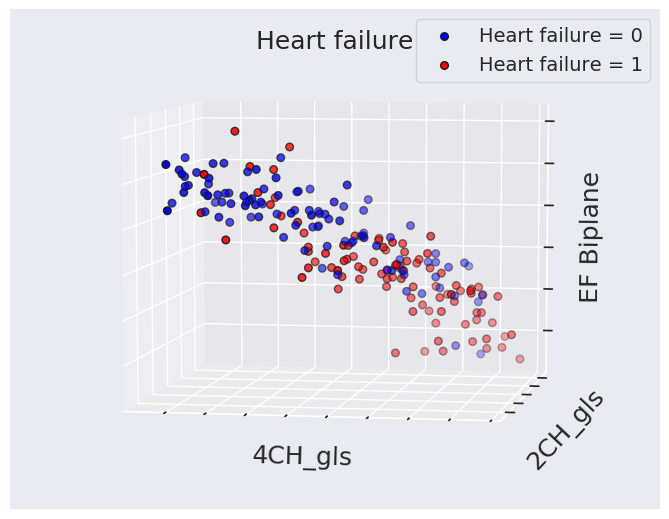
\includegraphics[width=0.99\textwidth]{results/hf/scatter_gls_EF_hf.png}
        \caption{Heart failure.}
        \label{fig:scatter_gls_ef_hf}
    \end{subfigure}
    \begin{subfigure}[b]{0.49\textwidth}
        \centering
        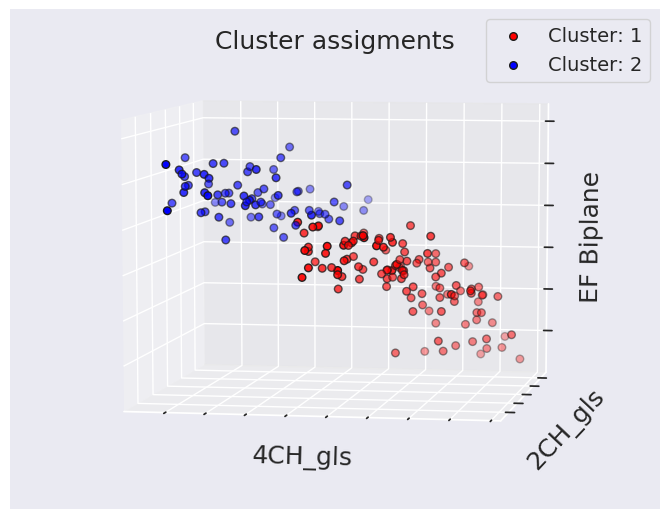
\includegraphics[width=0.99\textwidth]{results/hf/scatter_gls_EF_ward2.png}
        \caption{\textit{Ward/2} cluster assignments.}
        \label{fig:scatter_gls_ef_ward2}
    \end{subfigure}\\
    \begin{subfigure}[b]{0.49\textwidth}
        \centering
        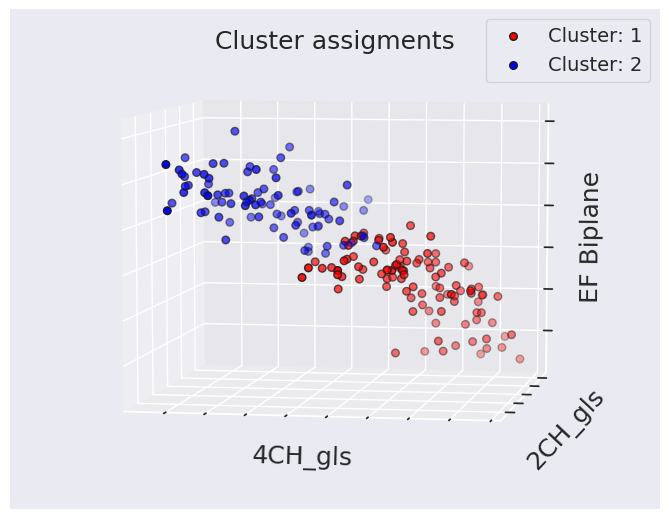
\includegraphics[width=0.99\textwidth]{results/hf/scatter_gls_EF_complete2.png}
        \caption{\textit{Complete/2} cluster assignments.}
        \label{fig:scatter_gls_ef_complete2}
    \end{subfigure}
    \begin{subfigure}[b]{0.49\textwidth}
        \centering
        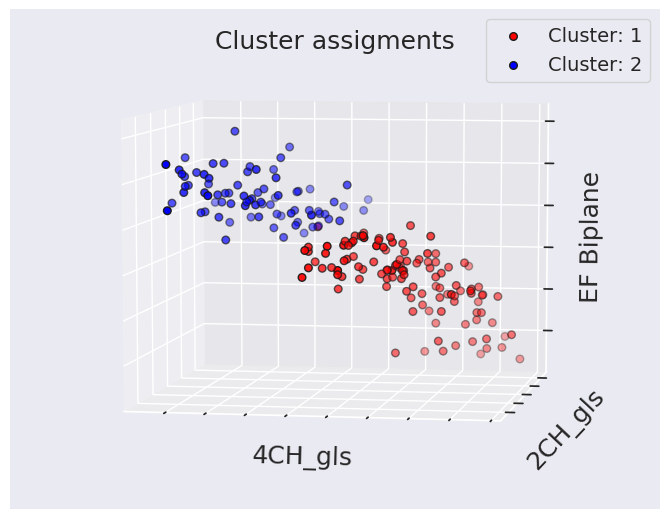
\includegraphics[width=0.99\textwidth]{results/hf/scatter_gls_EF_average2.png}
        \caption{\textit{Average/2} cluster assignments.}
        \label{fig:scatter_gls_ef_average2}
    \end{subfigure}
    \caption{Scatterplot of peak GLS values in each view. Colors in the of the different dots are given by heart failure diagnosis, and cluster assignments of 
             ward/2, complete/2 and average/2 methods. Numbers are not included on the axes because the point of the figure is to illustrate the separability 
             of clusters, and heart failure.}
             \label{fig:scatter_gls_ef_hf_cluster_assignments}
\end{figure}

\clearpage

\subsection{Deep Neural Network}

\begin{figure}[H]
    \centering
    % \includegraphics[width=\textwidth]{results/dl_hf_dor_sens_spec_dist.png}
    %% Creator: Matplotlib, PGF backend
%%
%% To include the figure in your LaTeX document, write
%%   \input{<filename>.pgf}
%%
%% Make sure the required packages are loaded in your preamble
%%   \usepackage{pgf}
%%
%% Figures using additional raster images can only be included by \input if
%% they are in the same directory as the main LaTeX file. For loading figures
%% from other directories you can use the `import` package
%%   \usepackage{import}
%% and then include the figures with
%%   \import{<path to file>}{<filename>.pgf}
%%
%% Matplotlib used the following preamble
%%
\begingroup%
\makeatletter%
\begin{pgfpicture}%
\pgfpathrectangle{\pgfpointorigin}{\pgfqpoint{6.246672in}{2.540000in}}%
\pgfusepath{use as bounding box, clip}%
\begin{pgfscope}%
\pgfsetbuttcap%
\pgfsetmiterjoin%
\definecolor{currentfill}{rgb}{1.000000,1.000000,1.000000}%
\pgfsetfillcolor{currentfill}%
\pgfsetlinewidth{0.000000pt}%
\definecolor{currentstroke}{rgb}{1.000000,1.000000,1.000000}%
\pgfsetstrokecolor{currentstroke}%
\pgfsetdash{}{0pt}%
\pgfpathmoveto{\pgfqpoint{0.000000in}{0.000000in}}%
\pgfpathlineto{\pgfqpoint{6.246672in}{0.000000in}}%
\pgfpathlineto{\pgfqpoint{6.246672in}{2.540000in}}%
\pgfpathlineto{\pgfqpoint{0.000000in}{2.540000in}}%
\pgfpathclose%
\pgfusepath{fill}%
\end{pgfscope}%
\begin{pgfscope}%
\pgfsetbuttcap%
\pgfsetmiterjoin%
\definecolor{currentfill}{rgb}{0.917647,0.917647,0.949020}%
\pgfsetfillcolor{currentfill}%
\pgfsetlinewidth{0.000000pt}%
\definecolor{currentstroke}{rgb}{0.000000,0.000000,0.000000}%
\pgfsetstrokecolor{currentstroke}%
\pgfsetstrokeopacity{0.000000}%
\pgfsetdash{}{0pt}%
\pgfpathmoveto{\pgfqpoint{0.574769in}{0.557870in}}%
\pgfpathlineto{\pgfqpoint{2.999734in}{0.557870in}}%
\pgfpathlineto{\pgfqpoint{2.999734in}{2.242604in}}%
\pgfpathlineto{\pgfqpoint{0.574769in}{2.242604in}}%
\pgfpathclose%
\pgfusepath{fill}%
\end{pgfscope}%
\begin{pgfscope}%
\pgfpathrectangle{\pgfqpoint{0.574769in}{0.557870in}}{\pgfqpoint{2.424965in}{1.684734in}}%
\pgfusepath{clip}%
\pgfsetroundcap%
\pgfsetroundjoin%
\pgfsetlinewidth{1.003750pt}%
\definecolor{currentstroke}{rgb}{1.000000,1.000000,1.000000}%
\pgfsetstrokecolor{currentstroke}%
\pgfsetdash{}{0pt}%
\pgfpathmoveto{\pgfqpoint{0.684994in}{0.557870in}}%
\pgfpathlineto{\pgfqpoint{0.684994in}{2.242604in}}%
\pgfusepath{stroke}%
\end{pgfscope}%
\begin{pgfscope}%
\definecolor{textcolor}{rgb}{0.150000,0.150000,0.150000}%
\pgfsetstrokecolor{textcolor}%
\pgfsetfillcolor{textcolor}%
\pgftext[x=0.684994in,y=0.425926in,,top]{\color{textcolor}\sffamily\fontsize{11.000000}{13.200000}\selectfont \(\displaystyle 0.0\)}%
\end{pgfscope}%
\begin{pgfscope}%
\pgfpathrectangle{\pgfqpoint{0.574769in}{0.557870in}}{\pgfqpoint{2.424965in}{1.684734in}}%
\pgfusepath{clip}%
\pgfsetroundcap%
\pgfsetroundjoin%
\pgfsetlinewidth{1.003750pt}%
\definecolor{currentstroke}{rgb}{1.000000,1.000000,1.000000}%
\pgfsetstrokecolor{currentstroke}%
\pgfsetdash{}{0pt}%
\pgfpathmoveto{\pgfqpoint{1.496956in}{0.557870in}}%
\pgfpathlineto{\pgfqpoint{1.496956in}{2.242604in}}%
\pgfusepath{stroke}%
\end{pgfscope}%
\begin{pgfscope}%
\definecolor{textcolor}{rgb}{0.150000,0.150000,0.150000}%
\pgfsetstrokecolor{textcolor}%
\pgfsetfillcolor{textcolor}%
\pgftext[x=1.496956in,y=0.425926in,,top]{\color{textcolor}\sffamily\fontsize{11.000000}{13.200000}\selectfont \(\displaystyle 0.5\)}%
\end{pgfscope}%
\begin{pgfscope}%
\pgfpathrectangle{\pgfqpoint{0.574769in}{0.557870in}}{\pgfqpoint{2.424965in}{1.684734in}}%
\pgfusepath{clip}%
\pgfsetroundcap%
\pgfsetroundjoin%
\pgfsetlinewidth{1.003750pt}%
\definecolor{currentstroke}{rgb}{1.000000,1.000000,1.000000}%
\pgfsetstrokecolor{currentstroke}%
\pgfsetdash{}{0pt}%
\pgfpathmoveto{\pgfqpoint{2.308918in}{0.557870in}}%
\pgfpathlineto{\pgfqpoint{2.308918in}{2.242604in}}%
\pgfusepath{stroke}%
\end{pgfscope}%
\begin{pgfscope}%
\definecolor{textcolor}{rgb}{0.150000,0.150000,0.150000}%
\pgfsetstrokecolor{textcolor}%
\pgfsetfillcolor{textcolor}%
\pgftext[x=2.308918in,y=0.425926in,,top]{\color{textcolor}\sffamily\fontsize{11.000000}{13.200000}\selectfont \(\displaystyle 1.0\)}%
\end{pgfscope}%
\begin{pgfscope}%
\definecolor{textcolor}{rgb}{0.150000,0.150000,0.150000}%
\pgfsetstrokecolor{textcolor}%
\pgfsetfillcolor{textcolor}%
\pgftext[x=1.787251in,y=0.235185in,,top]{\color{textcolor}\sffamily\fontsize{11.000000}{13.200000}\selectfont DOR}%
\end{pgfscope}%
\begin{pgfscope}%
\pgfpathrectangle{\pgfqpoint{0.574769in}{0.557870in}}{\pgfqpoint{2.424965in}{1.684734in}}%
\pgfusepath{clip}%
\pgfsetroundcap%
\pgfsetroundjoin%
\pgfsetlinewidth{1.003750pt}%
\definecolor{currentstroke}{rgb}{1.000000,1.000000,1.000000}%
\pgfsetstrokecolor{currentstroke}%
\pgfsetdash{}{0pt}%
\pgfpathmoveto{\pgfqpoint{0.574769in}{0.557870in}}%
\pgfpathlineto{\pgfqpoint{2.999734in}{0.557870in}}%
\pgfusepath{stroke}%
\end{pgfscope}%
\begin{pgfscope}%
\definecolor{textcolor}{rgb}{0.150000,0.150000,0.150000}%
\pgfsetstrokecolor{textcolor}%
\pgfsetfillcolor{textcolor}%
\pgftext[x=0.366783in,y=0.505064in,left,base]{\color{textcolor}\sffamily\fontsize{11.000000}{13.200000}\selectfont \(\displaystyle 0\)}%
\end{pgfscope}%
\begin{pgfscope}%
\pgfpathrectangle{\pgfqpoint{0.574769in}{0.557870in}}{\pgfqpoint{2.424965in}{1.684734in}}%
\pgfusepath{clip}%
\pgfsetroundcap%
\pgfsetroundjoin%
\pgfsetlinewidth{1.003750pt}%
\definecolor{currentstroke}{rgb}{1.000000,1.000000,1.000000}%
\pgfsetstrokecolor{currentstroke}%
\pgfsetdash{}{0pt}%
\pgfpathmoveto{\pgfqpoint{0.574769in}{1.174989in}}%
\pgfpathlineto{\pgfqpoint{2.999734in}{1.174989in}}%
\pgfusepath{stroke}%
\end{pgfscope}%
\begin{pgfscope}%
\definecolor{textcolor}{rgb}{0.150000,0.150000,0.150000}%
\pgfsetstrokecolor{textcolor}%
\pgfsetfillcolor{textcolor}%
\pgftext[x=0.366783in,y=1.122182in,left,base]{\color{textcolor}\sffamily\fontsize{11.000000}{13.200000}\selectfont \(\displaystyle 5\)}%
\end{pgfscope}%
\begin{pgfscope}%
\pgfpathrectangle{\pgfqpoint{0.574769in}{0.557870in}}{\pgfqpoint{2.424965in}{1.684734in}}%
\pgfusepath{clip}%
\pgfsetroundcap%
\pgfsetroundjoin%
\pgfsetlinewidth{1.003750pt}%
\definecolor{currentstroke}{rgb}{1.000000,1.000000,1.000000}%
\pgfsetstrokecolor{currentstroke}%
\pgfsetdash{}{0pt}%
\pgfpathmoveto{\pgfqpoint{0.574769in}{1.792108in}}%
\pgfpathlineto{\pgfqpoint{2.999734in}{1.792108in}}%
\pgfusepath{stroke}%
\end{pgfscope}%
\begin{pgfscope}%
\definecolor{textcolor}{rgb}{0.150000,0.150000,0.150000}%
\pgfsetstrokecolor{textcolor}%
\pgfsetfillcolor{textcolor}%
\pgftext[x=0.290741in,y=1.739301in,left,base]{\color{textcolor}\sffamily\fontsize{11.000000}{13.200000}\selectfont \(\displaystyle 10\)}%
\end{pgfscope}%
\begin{pgfscope}%
\definecolor{textcolor}{rgb}{0.150000,0.150000,0.150000}%
\pgfsetstrokecolor{textcolor}%
\pgfsetfillcolor{textcolor}%
\pgftext[x=0.235185in,y=1.400237in,,bottom,rotate=90.000000]{\color{textcolor}\sffamily\fontsize{11.000000}{13.200000}\selectfont Occurance}%
\end{pgfscope}%
\begin{pgfscope}%
\pgfpathrectangle{\pgfqpoint{0.574769in}{0.557870in}}{\pgfqpoint{2.424965in}{1.684734in}}%
\pgfusepath{clip}%
\pgfsetbuttcap%
\pgfsetmiterjoin%
\definecolor{currentfill}{rgb}{0.298039,0.447059,0.690196}%
\pgfsetfillcolor{currentfill}%
\pgfsetfillopacity{0.400000}%
\pgfsetlinewidth{1.003750pt}%
\definecolor{currentstroke}{rgb}{1.000000,1.000000,1.000000}%
\pgfsetstrokecolor{currentstroke}%
\pgfsetstrokeopacity{0.400000}%
\pgfsetdash{}{0pt}%
\pgfpathmoveto{\pgfqpoint{0.684994in}{0.557870in}}%
\pgfpathlineto{\pgfqpoint{0.905446in}{0.557870in}}%
\pgfpathlineto{\pgfqpoint{0.905446in}{2.162379in}}%
\pgfpathlineto{\pgfqpoint{0.684994in}{2.162379in}}%
\pgfpathclose%
\pgfusepath{stroke,fill}%
\end{pgfscope}%
\begin{pgfscope}%
\pgfpathrectangle{\pgfqpoint{0.574769in}{0.557870in}}{\pgfqpoint{2.424965in}{1.684734in}}%
\pgfusepath{clip}%
\pgfsetbuttcap%
\pgfsetmiterjoin%
\definecolor{currentfill}{rgb}{0.298039,0.447059,0.690196}%
\pgfsetfillcolor{currentfill}%
\pgfsetfillopacity{0.400000}%
\pgfsetlinewidth{1.003750pt}%
\definecolor{currentstroke}{rgb}{1.000000,1.000000,1.000000}%
\pgfsetstrokecolor{currentstroke}%
\pgfsetstrokeopacity{0.400000}%
\pgfsetdash{}{0pt}%
\pgfpathmoveto{\pgfqpoint{0.905446in}{0.557870in}}%
\pgfpathlineto{\pgfqpoint{1.125897in}{0.557870in}}%
\pgfpathlineto{\pgfqpoint{1.125897in}{1.174989in}}%
\pgfpathlineto{\pgfqpoint{0.905446in}{1.174989in}}%
\pgfpathclose%
\pgfusepath{stroke,fill}%
\end{pgfscope}%
\begin{pgfscope}%
\pgfpathrectangle{\pgfqpoint{0.574769in}{0.557870in}}{\pgfqpoint{2.424965in}{1.684734in}}%
\pgfusepath{clip}%
\pgfsetbuttcap%
\pgfsetmiterjoin%
\definecolor{currentfill}{rgb}{0.298039,0.447059,0.690196}%
\pgfsetfillcolor{currentfill}%
\pgfsetfillopacity{0.400000}%
\pgfsetlinewidth{1.003750pt}%
\definecolor{currentstroke}{rgb}{1.000000,1.000000,1.000000}%
\pgfsetstrokecolor{currentstroke}%
\pgfsetstrokeopacity{0.400000}%
\pgfsetdash{}{0pt}%
\pgfpathmoveto{\pgfqpoint{1.125897in}{0.557870in}}%
\pgfpathlineto{\pgfqpoint{1.346348in}{0.557870in}}%
\pgfpathlineto{\pgfqpoint{1.346348in}{1.298413in}}%
\pgfpathlineto{\pgfqpoint{1.125897in}{1.298413in}}%
\pgfpathclose%
\pgfusepath{stroke,fill}%
\end{pgfscope}%
\begin{pgfscope}%
\pgfpathrectangle{\pgfqpoint{0.574769in}{0.557870in}}{\pgfqpoint{2.424965in}{1.684734in}}%
\pgfusepath{clip}%
\pgfsetbuttcap%
\pgfsetmiterjoin%
\definecolor{currentfill}{rgb}{0.298039,0.447059,0.690196}%
\pgfsetfillcolor{currentfill}%
\pgfsetfillopacity{0.400000}%
\pgfsetlinewidth{1.003750pt}%
\definecolor{currentstroke}{rgb}{1.000000,1.000000,1.000000}%
\pgfsetstrokecolor{currentstroke}%
\pgfsetstrokeopacity{0.400000}%
\pgfsetdash{}{0pt}%
\pgfpathmoveto{\pgfqpoint{1.346348in}{0.557870in}}%
\pgfpathlineto{\pgfqpoint{1.566800in}{0.557870in}}%
\pgfpathlineto{\pgfqpoint{1.566800in}{0.928141in}}%
\pgfpathlineto{\pgfqpoint{1.346348in}{0.928141in}}%
\pgfpathclose%
\pgfusepath{stroke,fill}%
\end{pgfscope}%
\begin{pgfscope}%
\pgfpathrectangle{\pgfqpoint{0.574769in}{0.557870in}}{\pgfqpoint{2.424965in}{1.684734in}}%
\pgfusepath{clip}%
\pgfsetbuttcap%
\pgfsetmiterjoin%
\definecolor{currentfill}{rgb}{0.298039,0.447059,0.690196}%
\pgfsetfillcolor{currentfill}%
\pgfsetfillopacity{0.400000}%
\pgfsetlinewidth{1.003750pt}%
\definecolor{currentstroke}{rgb}{1.000000,1.000000,1.000000}%
\pgfsetstrokecolor{currentstroke}%
\pgfsetstrokeopacity{0.400000}%
\pgfsetdash{}{0pt}%
\pgfpathmoveto{\pgfqpoint{1.566800in}{0.557870in}}%
\pgfpathlineto{\pgfqpoint{1.787251in}{0.557870in}}%
\pgfpathlineto{\pgfqpoint{1.787251in}{0.557870in}}%
\pgfpathlineto{\pgfqpoint{1.566800in}{0.557870in}}%
\pgfpathclose%
\pgfusepath{stroke,fill}%
\end{pgfscope}%
\begin{pgfscope}%
\pgfpathrectangle{\pgfqpoint{0.574769in}{0.557870in}}{\pgfqpoint{2.424965in}{1.684734in}}%
\pgfusepath{clip}%
\pgfsetbuttcap%
\pgfsetmiterjoin%
\definecolor{currentfill}{rgb}{0.298039,0.447059,0.690196}%
\pgfsetfillcolor{currentfill}%
\pgfsetfillopacity{0.400000}%
\pgfsetlinewidth{1.003750pt}%
\definecolor{currentstroke}{rgb}{1.000000,1.000000,1.000000}%
\pgfsetstrokecolor{currentstroke}%
\pgfsetstrokeopacity{0.400000}%
\pgfsetdash{}{0pt}%
\pgfpathmoveto{\pgfqpoint{1.787251in}{0.557870in}}%
\pgfpathlineto{\pgfqpoint{2.007703in}{0.557870in}}%
\pgfpathlineto{\pgfqpoint{2.007703in}{0.681294in}}%
\pgfpathlineto{\pgfqpoint{1.787251in}{0.681294in}}%
\pgfpathclose%
\pgfusepath{stroke,fill}%
\end{pgfscope}%
\begin{pgfscope}%
\pgfpathrectangle{\pgfqpoint{0.574769in}{0.557870in}}{\pgfqpoint{2.424965in}{1.684734in}}%
\pgfusepath{clip}%
\pgfsetbuttcap%
\pgfsetmiterjoin%
\definecolor{currentfill}{rgb}{0.298039,0.447059,0.690196}%
\pgfsetfillcolor{currentfill}%
\pgfsetfillopacity{0.400000}%
\pgfsetlinewidth{1.003750pt}%
\definecolor{currentstroke}{rgb}{1.000000,1.000000,1.000000}%
\pgfsetstrokecolor{currentstroke}%
\pgfsetstrokeopacity{0.400000}%
\pgfsetdash{}{0pt}%
\pgfpathmoveto{\pgfqpoint{2.007703in}{0.557870in}}%
\pgfpathlineto{\pgfqpoint{2.228154in}{0.557870in}}%
\pgfpathlineto{\pgfqpoint{2.228154in}{0.804718in}}%
\pgfpathlineto{\pgfqpoint{2.007703in}{0.804718in}}%
\pgfpathclose%
\pgfusepath{stroke,fill}%
\end{pgfscope}%
\begin{pgfscope}%
\pgfpathrectangle{\pgfqpoint{0.574769in}{0.557870in}}{\pgfqpoint{2.424965in}{1.684734in}}%
\pgfusepath{clip}%
\pgfsetbuttcap%
\pgfsetmiterjoin%
\definecolor{currentfill}{rgb}{0.298039,0.447059,0.690196}%
\pgfsetfillcolor{currentfill}%
\pgfsetfillopacity{0.400000}%
\pgfsetlinewidth{1.003750pt}%
\definecolor{currentstroke}{rgb}{1.000000,1.000000,1.000000}%
\pgfsetstrokecolor{currentstroke}%
\pgfsetstrokeopacity{0.400000}%
\pgfsetdash{}{0pt}%
\pgfpathmoveto{\pgfqpoint{2.228154in}{0.557870in}}%
\pgfpathlineto{\pgfqpoint{2.448605in}{0.557870in}}%
\pgfpathlineto{\pgfqpoint{2.448605in}{0.804718in}}%
\pgfpathlineto{\pgfqpoint{2.228154in}{0.804718in}}%
\pgfpathclose%
\pgfusepath{stroke,fill}%
\end{pgfscope}%
\begin{pgfscope}%
\pgfpathrectangle{\pgfqpoint{0.574769in}{0.557870in}}{\pgfqpoint{2.424965in}{1.684734in}}%
\pgfusepath{clip}%
\pgfsetbuttcap%
\pgfsetmiterjoin%
\definecolor{currentfill}{rgb}{0.298039,0.447059,0.690196}%
\pgfsetfillcolor{currentfill}%
\pgfsetfillopacity{0.400000}%
\pgfsetlinewidth{1.003750pt}%
\definecolor{currentstroke}{rgb}{1.000000,1.000000,1.000000}%
\pgfsetstrokecolor{currentstroke}%
\pgfsetstrokeopacity{0.400000}%
\pgfsetdash{}{0pt}%
\pgfpathmoveto{\pgfqpoint{2.448605in}{0.557870in}}%
\pgfpathlineto{\pgfqpoint{2.669057in}{0.557870in}}%
\pgfpathlineto{\pgfqpoint{2.669057in}{0.804718in}}%
\pgfpathlineto{\pgfqpoint{2.448605in}{0.804718in}}%
\pgfpathclose%
\pgfusepath{stroke,fill}%
\end{pgfscope}%
\begin{pgfscope}%
\pgfpathrectangle{\pgfqpoint{0.574769in}{0.557870in}}{\pgfqpoint{2.424965in}{1.684734in}}%
\pgfusepath{clip}%
\pgfsetbuttcap%
\pgfsetmiterjoin%
\definecolor{currentfill}{rgb}{0.298039,0.447059,0.690196}%
\pgfsetfillcolor{currentfill}%
\pgfsetfillopacity{0.400000}%
\pgfsetlinewidth{1.003750pt}%
\definecolor{currentstroke}{rgb}{1.000000,1.000000,1.000000}%
\pgfsetstrokecolor{currentstroke}%
\pgfsetstrokeopacity{0.400000}%
\pgfsetdash{}{0pt}%
\pgfpathmoveto{\pgfqpoint{2.669057in}{0.557870in}}%
\pgfpathlineto{\pgfqpoint{2.889508in}{0.557870in}}%
\pgfpathlineto{\pgfqpoint{2.889508in}{0.804718in}}%
\pgfpathlineto{\pgfqpoint{2.669057in}{0.804718in}}%
\pgfpathclose%
\pgfusepath{stroke,fill}%
\end{pgfscope}%
\begin{pgfscope}%
\pgfsetrectcap%
\pgfsetmiterjoin%
\pgfsetlinewidth{1.254687pt}%
\definecolor{currentstroke}{rgb}{1.000000,1.000000,1.000000}%
\pgfsetstrokecolor{currentstroke}%
\pgfsetdash{}{0pt}%
\pgfpathmoveto{\pgfqpoint{0.574769in}{0.557870in}}%
\pgfpathlineto{\pgfqpoint{0.574769in}{2.242604in}}%
\pgfusepath{stroke}%
\end{pgfscope}%
\begin{pgfscope}%
\pgfsetrectcap%
\pgfsetmiterjoin%
\pgfsetlinewidth{1.254687pt}%
\definecolor{currentstroke}{rgb}{1.000000,1.000000,1.000000}%
\pgfsetstrokecolor{currentstroke}%
\pgfsetdash{}{0pt}%
\pgfpathmoveto{\pgfqpoint{2.999734in}{0.557870in}}%
\pgfpathlineto{\pgfqpoint{2.999734in}{2.242604in}}%
\pgfusepath{stroke}%
\end{pgfscope}%
\begin{pgfscope}%
\pgfsetrectcap%
\pgfsetmiterjoin%
\pgfsetlinewidth{1.254687pt}%
\definecolor{currentstroke}{rgb}{1.000000,1.000000,1.000000}%
\pgfsetstrokecolor{currentstroke}%
\pgfsetdash{}{0pt}%
\pgfpathmoveto{\pgfqpoint{0.574769in}{0.557870in}}%
\pgfpathlineto{\pgfqpoint{2.999734in}{0.557870in}}%
\pgfusepath{stroke}%
\end{pgfscope}%
\begin{pgfscope}%
\pgfsetrectcap%
\pgfsetmiterjoin%
\pgfsetlinewidth{1.254687pt}%
\definecolor{currentstroke}{rgb}{1.000000,1.000000,1.000000}%
\pgfsetstrokecolor{currentstroke}%
\pgfsetdash{}{0pt}%
\pgfpathmoveto{\pgfqpoint{0.574769in}{2.242604in}}%
\pgfpathlineto{\pgfqpoint{2.999734in}{2.242604in}}%
\pgfusepath{stroke}%
\end{pgfscope}%
\begin{pgfscope}%
\definecolor{textcolor}{rgb}{0.150000,0.150000,0.150000}%
\pgfsetstrokecolor{textcolor}%
\pgfsetfillcolor{textcolor}%
\pgftext[x=1.787251in,y=2.325938in,,base]{\color{textcolor}\sffamily\fontsize{11.000000}{13.200000}\selectfont (a)}%
\end{pgfscope}%
\begin{pgfscope}%
\pgfsetbuttcap%
\pgfsetmiterjoin%
\definecolor{currentfill}{rgb}{0.917647,0.917647,0.949020}%
\pgfsetfillcolor{currentfill}%
\pgfsetlinewidth{0.000000pt}%
\definecolor{currentstroke}{rgb}{0.000000,0.000000,0.000000}%
\pgfsetstrokecolor{currentstroke}%
\pgfsetstrokeopacity{0.000000}%
\pgfsetdash{}{0pt}%
\pgfpathmoveto{\pgfqpoint{3.696748in}{0.557870in}}%
\pgfpathlineto{\pgfqpoint{6.121713in}{0.557870in}}%
\pgfpathlineto{\pgfqpoint{6.121713in}{2.242604in}}%
\pgfpathlineto{\pgfqpoint{3.696748in}{2.242604in}}%
\pgfpathclose%
\pgfusepath{fill}%
\end{pgfscope}%
\begin{pgfscope}%
\pgfpathrectangle{\pgfqpoint{3.696748in}{0.557870in}}{\pgfqpoint{2.424965in}{1.684734in}}%
\pgfusepath{clip}%
\pgfsetroundcap%
\pgfsetroundjoin%
\pgfsetlinewidth{1.003750pt}%
\definecolor{currentstroke}{rgb}{1.000000,1.000000,1.000000}%
\pgfsetstrokecolor{currentstroke}%
\pgfsetdash{}{0pt}%
\pgfpathmoveto{\pgfqpoint{3.806973in}{0.557870in}}%
\pgfpathlineto{\pgfqpoint{3.806973in}{2.242604in}}%
\pgfusepath{stroke}%
\end{pgfscope}%
\begin{pgfscope}%
\definecolor{textcolor}{rgb}{0.150000,0.150000,0.150000}%
\pgfsetstrokecolor{textcolor}%
\pgfsetfillcolor{textcolor}%
\pgftext[x=3.806973in,y=0.425926in,,top]{\color{textcolor}\sffamily\fontsize{11.000000}{13.200000}\selectfont \(\displaystyle 0.00\)}%
\end{pgfscope}%
\begin{pgfscope}%
\pgfpathrectangle{\pgfqpoint{3.696748in}{0.557870in}}{\pgfqpoint{2.424965in}{1.684734in}}%
\pgfusepath{clip}%
\pgfsetroundcap%
\pgfsetroundjoin%
\pgfsetlinewidth{1.003750pt}%
\definecolor{currentstroke}{rgb}{1.000000,1.000000,1.000000}%
\pgfsetstrokecolor{currentstroke}%
\pgfsetdash{}{0pt}%
\pgfpathmoveto{\pgfqpoint{4.358102in}{0.557870in}}%
\pgfpathlineto{\pgfqpoint{4.358102in}{2.242604in}}%
\pgfusepath{stroke}%
\end{pgfscope}%
\begin{pgfscope}%
\definecolor{textcolor}{rgb}{0.150000,0.150000,0.150000}%
\pgfsetstrokecolor{textcolor}%
\pgfsetfillcolor{textcolor}%
\pgftext[x=4.358102in,y=0.425926in,,top]{\color{textcolor}\sffamily\fontsize{11.000000}{13.200000}\selectfont \(\displaystyle 0.25\)}%
\end{pgfscope}%
\begin{pgfscope}%
\pgfpathrectangle{\pgfqpoint{3.696748in}{0.557870in}}{\pgfqpoint{2.424965in}{1.684734in}}%
\pgfusepath{clip}%
\pgfsetroundcap%
\pgfsetroundjoin%
\pgfsetlinewidth{1.003750pt}%
\definecolor{currentstroke}{rgb}{1.000000,1.000000,1.000000}%
\pgfsetstrokecolor{currentstroke}%
\pgfsetdash{}{0pt}%
\pgfpathmoveto{\pgfqpoint{4.909230in}{0.557870in}}%
\pgfpathlineto{\pgfqpoint{4.909230in}{2.242604in}}%
\pgfusepath{stroke}%
\end{pgfscope}%
\begin{pgfscope}%
\definecolor{textcolor}{rgb}{0.150000,0.150000,0.150000}%
\pgfsetstrokecolor{textcolor}%
\pgfsetfillcolor{textcolor}%
\pgftext[x=4.909230in,y=0.425926in,,top]{\color{textcolor}\sffamily\fontsize{11.000000}{13.200000}\selectfont \(\displaystyle 0.50\)}%
\end{pgfscope}%
\begin{pgfscope}%
\pgfpathrectangle{\pgfqpoint{3.696748in}{0.557870in}}{\pgfqpoint{2.424965in}{1.684734in}}%
\pgfusepath{clip}%
\pgfsetroundcap%
\pgfsetroundjoin%
\pgfsetlinewidth{1.003750pt}%
\definecolor{currentstroke}{rgb}{1.000000,1.000000,1.000000}%
\pgfsetstrokecolor{currentstroke}%
\pgfsetdash{}{0pt}%
\pgfpathmoveto{\pgfqpoint{5.460359in}{0.557870in}}%
\pgfpathlineto{\pgfqpoint{5.460359in}{2.242604in}}%
\pgfusepath{stroke}%
\end{pgfscope}%
\begin{pgfscope}%
\definecolor{textcolor}{rgb}{0.150000,0.150000,0.150000}%
\pgfsetstrokecolor{textcolor}%
\pgfsetfillcolor{textcolor}%
\pgftext[x=5.460359in,y=0.425926in,,top]{\color{textcolor}\sffamily\fontsize{11.000000}{13.200000}\selectfont \(\displaystyle 0.75\)}%
\end{pgfscope}%
\begin{pgfscope}%
\pgfpathrectangle{\pgfqpoint{3.696748in}{0.557870in}}{\pgfqpoint{2.424965in}{1.684734in}}%
\pgfusepath{clip}%
\pgfsetroundcap%
\pgfsetroundjoin%
\pgfsetlinewidth{1.003750pt}%
\definecolor{currentstroke}{rgb}{1.000000,1.000000,1.000000}%
\pgfsetstrokecolor{currentstroke}%
\pgfsetdash{}{0pt}%
\pgfpathmoveto{\pgfqpoint{6.011487in}{0.557870in}}%
\pgfpathlineto{\pgfqpoint{6.011487in}{2.242604in}}%
\pgfusepath{stroke}%
\end{pgfscope}%
\begin{pgfscope}%
\definecolor{textcolor}{rgb}{0.150000,0.150000,0.150000}%
\pgfsetstrokecolor{textcolor}%
\pgfsetfillcolor{textcolor}%
\pgftext[x=6.011487in,y=0.425926in,,top]{\color{textcolor}\sffamily\fontsize{11.000000}{13.200000}\selectfont \(\displaystyle 1.00\)}%
\end{pgfscope}%
\begin{pgfscope}%
\definecolor{textcolor}{rgb}{0.150000,0.150000,0.150000}%
\pgfsetstrokecolor{textcolor}%
\pgfsetfillcolor{textcolor}%
\pgftext[x=4.909230in,y=0.235185in,,top]{\color{textcolor}\sffamily\fontsize{11.000000}{13.200000}\selectfont Specificity}%
\end{pgfscope}%
\begin{pgfscope}%
\pgfpathrectangle{\pgfqpoint{3.696748in}{0.557870in}}{\pgfqpoint{2.424965in}{1.684734in}}%
\pgfusepath{clip}%
\pgfsetroundcap%
\pgfsetroundjoin%
\pgfsetlinewidth{1.003750pt}%
\definecolor{currentstroke}{rgb}{1.000000,1.000000,1.000000}%
\pgfsetstrokecolor{currentstroke}%
\pgfsetdash{}{0pt}%
\pgfpathmoveto{\pgfqpoint{3.696748in}{0.634449in}}%
\pgfpathlineto{\pgfqpoint{6.121713in}{0.634449in}}%
\pgfusepath{stroke}%
\end{pgfscope}%
\begin{pgfscope}%
\definecolor{textcolor}{rgb}{0.150000,0.150000,0.150000}%
\pgfsetstrokecolor{textcolor}%
\pgfsetfillcolor{textcolor}%
\pgftext[x=3.294433in,y=0.581642in,left,base]{\color{textcolor}\sffamily\fontsize{11.000000}{13.200000}\selectfont \(\displaystyle 0.00\)}%
\end{pgfscope}%
\begin{pgfscope}%
\pgfpathrectangle{\pgfqpoint{3.696748in}{0.557870in}}{\pgfqpoint{2.424965in}{1.684734in}}%
\pgfusepath{clip}%
\pgfsetroundcap%
\pgfsetroundjoin%
\pgfsetlinewidth{1.003750pt}%
\definecolor{currentstroke}{rgb}{1.000000,1.000000,1.000000}%
\pgfsetstrokecolor{currentstroke}%
\pgfsetdash{}{0pt}%
\pgfpathmoveto{\pgfqpoint{3.696748in}{1.017343in}}%
\pgfpathlineto{\pgfqpoint{6.121713in}{1.017343in}}%
\pgfusepath{stroke}%
\end{pgfscope}%
\begin{pgfscope}%
\definecolor{textcolor}{rgb}{0.150000,0.150000,0.150000}%
\pgfsetstrokecolor{textcolor}%
\pgfsetfillcolor{textcolor}%
\pgftext[x=3.294433in,y=0.964536in,left,base]{\color{textcolor}\sffamily\fontsize{11.000000}{13.200000}\selectfont \(\displaystyle 0.25\)}%
\end{pgfscope}%
\begin{pgfscope}%
\pgfpathrectangle{\pgfqpoint{3.696748in}{0.557870in}}{\pgfqpoint{2.424965in}{1.684734in}}%
\pgfusepath{clip}%
\pgfsetroundcap%
\pgfsetroundjoin%
\pgfsetlinewidth{1.003750pt}%
\definecolor{currentstroke}{rgb}{1.000000,1.000000,1.000000}%
\pgfsetstrokecolor{currentstroke}%
\pgfsetdash{}{0pt}%
\pgfpathmoveto{\pgfqpoint{3.696748in}{1.400237in}}%
\pgfpathlineto{\pgfqpoint{6.121713in}{1.400237in}}%
\pgfusepath{stroke}%
\end{pgfscope}%
\begin{pgfscope}%
\definecolor{textcolor}{rgb}{0.150000,0.150000,0.150000}%
\pgfsetstrokecolor{textcolor}%
\pgfsetfillcolor{textcolor}%
\pgftext[x=3.294433in,y=1.347431in,left,base]{\color{textcolor}\sffamily\fontsize{11.000000}{13.200000}\selectfont \(\displaystyle 0.50\)}%
\end{pgfscope}%
\begin{pgfscope}%
\pgfpathrectangle{\pgfqpoint{3.696748in}{0.557870in}}{\pgfqpoint{2.424965in}{1.684734in}}%
\pgfusepath{clip}%
\pgfsetroundcap%
\pgfsetroundjoin%
\pgfsetlinewidth{1.003750pt}%
\definecolor{currentstroke}{rgb}{1.000000,1.000000,1.000000}%
\pgfsetstrokecolor{currentstroke}%
\pgfsetdash{}{0pt}%
\pgfpathmoveto{\pgfqpoint{3.696748in}{1.783131in}}%
\pgfpathlineto{\pgfqpoint{6.121713in}{1.783131in}}%
\pgfusepath{stroke}%
\end{pgfscope}%
\begin{pgfscope}%
\definecolor{textcolor}{rgb}{0.150000,0.150000,0.150000}%
\pgfsetstrokecolor{textcolor}%
\pgfsetfillcolor{textcolor}%
\pgftext[x=3.294433in,y=1.730325in,left,base]{\color{textcolor}\sffamily\fontsize{11.000000}{13.200000}\selectfont \(\displaystyle 0.75\)}%
\end{pgfscope}%
\begin{pgfscope}%
\pgfpathrectangle{\pgfqpoint{3.696748in}{0.557870in}}{\pgfqpoint{2.424965in}{1.684734in}}%
\pgfusepath{clip}%
\pgfsetroundcap%
\pgfsetroundjoin%
\pgfsetlinewidth{1.003750pt}%
\definecolor{currentstroke}{rgb}{1.000000,1.000000,1.000000}%
\pgfsetstrokecolor{currentstroke}%
\pgfsetdash{}{0pt}%
\pgfpathmoveto{\pgfqpoint{3.696748in}{2.166025in}}%
\pgfpathlineto{\pgfqpoint{6.121713in}{2.166025in}}%
\pgfusepath{stroke}%
\end{pgfscope}%
\begin{pgfscope}%
\definecolor{textcolor}{rgb}{0.150000,0.150000,0.150000}%
\pgfsetstrokecolor{textcolor}%
\pgfsetfillcolor{textcolor}%
\pgftext[x=3.294433in,y=2.113219in,left,base]{\color{textcolor}\sffamily\fontsize{11.000000}{13.200000}\selectfont \(\displaystyle 1.00\)}%
\end{pgfscope}%
\begin{pgfscope}%
\definecolor{textcolor}{rgb}{0.150000,0.150000,0.150000}%
\pgfsetstrokecolor{textcolor}%
\pgfsetfillcolor{textcolor}%
\pgftext[x=3.238877in,y=1.400237in,,bottom,rotate=90.000000]{\color{textcolor}\sffamily\fontsize{11.000000}{13.200000}\selectfont Sensitivity}%
\end{pgfscope}%
\begin{pgfscope}%
\pgfpathrectangle{\pgfqpoint{3.696748in}{0.557870in}}{\pgfqpoint{2.424965in}{1.684734in}}%
\pgfusepath{clip}%
\pgfsetbuttcap%
\pgfsetroundjoin%
\definecolor{currentfill}{rgb}{0.298039,0.447059,0.690196}%
\pgfsetfillcolor{currentfill}%
\pgfsetlinewidth{1.003750pt}%
\definecolor{currentstroke}{rgb}{0.298039,0.447059,0.690196}%
\pgfsetstrokecolor{currentstroke}%
\pgfsetdash{}{0pt}%
\pgfpathmoveto{\pgfqpoint{5.151727in}{1.315034in}}%
\pgfpathcurveto{\pgfqpoint{5.159963in}{1.315034in}}{\pgfqpoint{5.167863in}{1.318306in}}{\pgfqpoint{5.173687in}{1.324130in}}%
\pgfpathcurveto{\pgfqpoint{5.179511in}{1.329954in}}{\pgfqpoint{5.182783in}{1.337854in}}{\pgfqpoint{5.182783in}{1.346091in}}%
\pgfpathcurveto{\pgfqpoint{5.182783in}{1.354327in}}{\pgfqpoint{5.179511in}{1.362227in}}{\pgfqpoint{5.173687in}{1.368051in}}%
\pgfpathcurveto{\pgfqpoint{5.167863in}{1.373875in}}{\pgfqpoint{5.159963in}{1.377147in}}{\pgfqpoint{5.151727in}{1.377147in}}%
\pgfpathcurveto{\pgfqpoint{5.143490in}{1.377147in}}{\pgfqpoint{5.135590in}{1.373875in}}{\pgfqpoint{5.129766in}{1.368051in}}%
\pgfpathcurveto{\pgfqpoint{5.123943in}{1.362227in}}{\pgfqpoint{5.120670in}{1.354327in}}{\pgfqpoint{5.120670in}{1.346091in}}%
\pgfpathcurveto{\pgfqpoint{5.120670in}{1.337854in}}{\pgfqpoint{5.123943in}{1.329954in}}{\pgfqpoint{5.129766in}{1.324130in}}%
\pgfpathcurveto{\pgfqpoint{5.135590in}{1.318306in}}{\pgfqpoint{5.143490in}{1.315034in}}{\pgfqpoint{5.151727in}{1.315034in}}%
\pgfpathclose%
\pgfusepath{stroke,fill}%
\end{pgfscope}%
\begin{pgfscope}%
\pgfpathrectangle{\pgfqpoint{3.696748in}{0.557870in}}{\pgfqpoint{2.424965in}{1.684734in}}%
\pgfusepath{clip}%
\pgfsetbuttcap%
\pgfsetroundjoin%
\definecolor{currentfill}{rgb}{0.298039,0.447059,0.690196}%
\pgfsetfillcolor{currentfill}%
\pgfsetlinewidth{1.003750pt}%
\definecolor{currentstroke}{rgb}{0.298039,0.447059,0.690196}%
\pgfsetstrokecolor{currentstroke}%
\pgfsetdash{}{0pt}%
\pgfpathmoveto{\pgfqpoint{5.085591in}{1.345975in}}%
\pgfpathcurveto{\pgfqpoint{5.093828in}{1.345975in}}{\pgfqpoint{5.101728in}{1.349247in}}{\pgfqpoint{5.107552in}{1.355071in}}%
\pgfpathcurveto{\pgfqpoint{5.113376in}{1.360895in}}{\pgfqpoint{5.116648in}{1.368795in}}{\pgfqpoint{5.116648in}{1.377032in}}%
\pgfpathcurveto{\pgfqpoint{5.116648in}{1.385268in}}{\pgfqpoint{5.113376in}{1.393168in}}{\pgfqpoint{5.107552in}{1.398992in}}%
\pgfpathcurveto{\pgfqpoint{5.101728in}{1.404816in}}{\pgfqpoint{5.093828in}{1.408088in}}{\pgfqpoint{5.085591in}{1.408088in}}%
\pgfpathcurveto{\pgfqpoint{5.077355in}{1.408088in}}{\pgfqpoint{5.069455in}{1.404816in}}{\pgfqpoint{5.063631in}{1.398992in}}%
\pgfpathcurveto{\pgfqpoint{5.057807in}{1.393168in}}{\pgfqpoint{5.054535in}{1.385268in}}{\pgfqpoint{5.054535in}{1.377032in}}%
\pgfpathcurveto{\pgfqpoint{5.054535in}{1.368795in}}{\pgfqpoint{5.057807in}{1.360895in}}{\pgfqpoint{5.063631in}{1.355071in}}%
\pgfpathcurveto{\pgfqpoint{5.069455in}{1.349247in}}{\pgfqpoint{5.077355in}{1.345975in}}{\pgfqpoint{5.085591in}{1.345975in}}%
\pgfpathclose%
\pgfusepath{stroke,fill}%
\end{pgfscope}%
\begin{pgfscope}%
\pgfpathrectangle{\pgfqpoint{3.696748in}{0.557870in}}{\pgfqpoint{2.424965in}{1.684734in}}%
\pgfusepath{clip}%
\pgfsetbuttcap%
\pgfsetroundjoin%
\definecolor{currentfill}{rgb}{0.298039,0.447059,0.690196}%
\pgfsetfillcolor{currentfill}%
\pgfsetlinewidth{1.003750pt}%
\definecolor{currentstroke}{rgb}{0.298039,0.447059,0.690196}%
\pgfsetstrokecolor{currentstroke}%
\pgfsetdash{}{0pt}%
\pgfpathmoveto{\pgfqpoint{5.306043in}{1.154760in}}%
\pgfpathcurveto{\pgfqpoint{5.314279in}{1.154760in}}{\pgfqpoint{5.322179in}{1.158032in}}{\pgfqpoint{5.328003in}{1.163856in}}%
\pgfpathcurveto{\pgfqpoint{5.333827in}{1.169680in}}{\pgfqpoint{5.337099in}{1.177580in}}{\pgfqpoint{5.337099in}{1.185817in}}%
\pgfpathcurveto{\pgfqpoint{5.337099in}{1.194053in}}{\pgfqpoint{5.333827in}{1.201953in}}{\pgfqpoint{5.328003in}{1.207777in}}%
\pgfpathcurveto{\pgfqpoint{5.322179in}{1.213601in}}{\pgfqpoint{5.314279in}{1.216873in}}{\pgfqpoint{5.306043in}{1.216873in}}%
\pgfpathcurveto{\pgfqpoint{5.297806in}{1.216873in}}{\pgfqpoint{5.289906in}{1.213601in}}{\pgfqpoint{5.284082in}{1.207777in}}%
\pgfpathcurveto{\pgfqpoint{5.278259in}{1.201953in}}{\pgfqpoint{5.274986in}{1.194053in}}{\pgfqpoint{5.274986in}{1.185817in}}%
\pgfpathcurveto{\pgfqpoint{5.274986in}{1.177580in}}{\pgfqpoint{5.278259in}{1.169680in}}{\pgfqpoint{5.284082in}{1.163856in}}%
\pgfpathcurveto{\pgfqpoint{5.289906in}{1.158032in}}{\pgfqpoint{5.297806in}{1.154760in}}{\pgfqpoint{5.306043in}{1.154760in}}%
\pgfpathclose%
\pgfusepath{stroke,fill}%
\end{pgfscope}%
\begin{pgfscope}%
\pgfpathrectangle{\pgfqpoint{3.696748in}{0.557870in}}{\pgfqpoint{2.424965in}{1.684734in}}%
\pgfusepath{clip}%
\pgfsetbuttcap%
\pgfsetroundjoin%
\definecolor{currentfill}{rgb}{0.298039,0.447059,0.690196}%
\pgfsetfillcolor{currentfill}%
\pgfsetlinewidth{1.003750pt}%
\definecolor{currentstroke}{rgb}{0.298039,0.447059,0.690196}%
\pgfsetstrokecolor{currentstroke}%
\pgfsetdash{}{0pt}%
\pgfpathmoveto{\pgfqpoint{4.688779in}{1.572349in}}%
\pgfpathcurveto{\pgfqpoint{4.697015in}{1.572349in}}{\pgfqpoint{4.704915in}{1.575621in}}{\pgfqpoint{4.710739in}{1.581445in}}%
\pgfpathcurveto{\pgfqpoint{4.716563in}{1.587269in}}{\pgfqpoint{4.719835in}{1.595169in}}{\pgfqpoint{4.719835in}{1.603406in}}%
\pgfpathcurveto{\pgfqpoint{4.719835in}{1.611642in}}{\pgfqpoint{4.716563in}{1.619542in}}{\pgfqpoint{4.710739in}{1.625366in}}%
\pgfpathcurveto{\pgfqpoint{4.704915in}{1.631190in}}{\pgfqpoint{4.697015in}{1.634462in}}{\pgfqpoint{4.688779in}{1.634462in}}%
\pgfpathcurveto{\pgfqpoint{4.680543in}{1.634462in}}{\pgfqpoint{4.672643in}{1.631190in}}{\pgfqpoint{4.666819in}{1.625366in}}%
\pgfpathcurveto{\pgfqpoint{4.660995in}{1.619542in}}{\pgfqpoint{4.657722in}{1.611642in}}{\pgfqpoint{4.657722in}{1.603406in}}%
\pgfpathcurveto{\pgfqpoint{4.657722in}{1.595169in}}{\pgfqpoint{4.660995in}{1.587269in}}{\pgfqpoint{4.666819in}{1.581445in}}%
\pgfpathcurveto{\pgfqpoint{4.672643in}{1.575621in}}{\pgfqpoint{4.680543in}{1.572349in}}{\pgfqpoint{4.688779in}{1.572349in}}%
\pgfpathclose%
\pgfusepath{stroke,fill}%
\end{pgfscope}%
\begin{pgfscope}%
\pgfpathrectangle{\pgfqpoint{3.696748in}{0.557870in}}{\pgfqpoint{2.424965in}{1.684734in}}%
\pgfusepath{clip}%
\pgfsetbuttcap%
\pgfsetroundjoin%
\definecolor{currentfill}{rgb}{0.298039,0.447059,0.690196}%
\pgfsetfillcolor{currentfill}%
\pgfsetlinewidth{1.003750pt}%
\definecolor{currentstroke}{rgb}{0.298039,0.447059,0.690196}%
\pgfsetstrokecolor{currentstroke}%
\pgfsetdash{}{0pt}%
\pgfpathmoveto{\pgfqpoint{4.693324in}{1.531621in}}%
\pgfpathcurveto{\pgfqpoint{4.701561in}{1.531621in}}{\pgfqpoint{4.709461in}{1.534893in}}{\pgfqpoint{4.715285in}{1.540717in}}%
\pgfpathcurveto{\pgfqpoint{4.721108in}{1.546541in}}{\pgfqpoint{4.724381in}{1.554441in}}{\pgfqpoint{4.724381in}{1.562677in}}%
\pgfpathcurveto{\pgfqpoint{4.724381in}{1.570913in}}{\pgfqpoint{4.721108in}{1.578813in}}{\pgfqpoint{4.715285in}{1.584637in}}%
\pgfpathcurveto{\pgfqpoint{4.709461in}{1.590461in}}{\pgfqpoint{4.701561in}{1.593734in}}{\pgfqpoint{4.693324in}{1.593734in}}%
\pgfpathcurveto{\pgfqpoint{4.685088in}{1.593734in}}{\pgfqpoint{4.677188in}{1.590461in}}{\pgfqpoint{4.671364in}{1.584637in}}%
\pgfpathcurveto{\pgfqpoint{4.665540in}{1.578813in}}{\pgfqpoint{4.662268in}{1.570913in}}{\pgfqpoint{4.662268in}{1.562677in}}%
\pgfpathcurveto{\pgfqpoint{4.662268in}{1.554441in}}{\pgfqpoint{4.665540in}{1.546541in}}{\pgfqpoint{4.671364in}{1.540717in}}%
\pgfpathcurveto{\pgfqpoint{4.677188in}{1.534893in}}{\pgfqpoint{4.685088in}{1.531621in}}{\pgfqpoint{4.693324in}{1.531621in}}%
\pgfpathclose%
\pgfusepath{stroke,fill}%
\end{pgfscope}%
\begin{pgfscope}%
\pgfpathrectangle{\pgfqpoint{3.696748in}{0.557870in}}{\pgfqpoint{2.424965in}{1.684734in}}%
\pgfusepath{clip}%
\pgfsetbuttcap%
\pgfsetroundjoin%
\definecolor{currentfill}{rgb}{0.298039,0.447059,0.690196}%
\pgfsetfillcolor{currentfill}%
\pgfsetlinewidth{1.003750pt}%
\definecolor{currentstroke}{rgb}{0.298039,0.447059,0.690196}%
\pgfsetstrokecolor{currentstroke}%
\pgfsetdash{}{0pt}%
\pgfpathmoveto{\pgfqpoint{4.953321in}{1.345975in}}%
\pgfpathcurveto{\pgfqpoint{4.961557in}{1.345975in}}{\pgfqpoint{4.969457in}{1.349247in}}{\pgfqpoint{4.975281in}{1.355071in}}%
\pgfpathcurveto{\pgfqpoint{4.981105in}{1.360895in}}{\pgfqpoint{4.984377in}{1.368795in}}{\pgfqpoint{4.984377in}{1.377032in}}%
\pgfpathcurveto{\pgfqpoint{4.984377in}{1.385268in}}{\pgfqpoint{4.981105in}{1.393168in}}{\pgfqpoint{4.975281in}{1.398992in}}%
\pgfpathcurveto{\pgfqpoint{4.969457in}{1.404816in}}{\pgfqpoint{4.961557in}{1.408088in}}{\pgfqpoint{4.953321in}{1.408088in}}%
\pgfpathcurveto{\pgfqpoint{4.945084in}{1.408088in}}{\pgfqpoint{4.937184in}{1.404816in}}{\pgfqpoint{4.931360in}{1.398992in}}%
\pgfpathcurveto{\pgfqpoint{4.925536in}{1.393168in}}{\pgfqpoint{4.922264in}{1.385268in}}{\pgfqpoint{4.922264in}{1.377032in}}%
\pgfpathcurveto{\pgfqpoint{4.922264in}{1.368795in}}{\pgfqpoint{4.925536in}{1.360895in}}{\pgfqpoint{4.931360in}{1.355071in}}%
\pgfpathcurveto{\pgfqpoint{4.937184in}{1.349247in}}{\pgfqpoint{4.945084in}{1.345975in}}{\pgfqpoint{4.953321in}{1.345975in}}%
\pgfpathclose%
\pgfusepath{stroke,fill}%
\end{pgfscope}%
\begin{pgfscope}%
\pgfpathrectangle{\pgfqpoint{3.696748in}{0.557870in}}{\pgfqpoint{2.424965in}{1.684734in}}%
\pgfusepath{clip}%
\pgfsetbuttcap%
\pgfsetroundjoin%
\definecolor{currentfill}{rgb}{0.298039,0.447059,0.690196}%
\pgfsetfillcolor{currentfill}%
\pgfsetlinewidth{1.003750pt}%
\definecolor{currentstroke}{rgb}{0.298039,0.447059,0.690196}%
\pgfsetstrokecolor{currentstroke}%
\pgfsetdash{}{0pt}%
\pgfpathmoveto{\pgfqpoint{4.909230in}{1.345975in}}%
\pgfpathcurveto{\pgfqpoint{4.917467in}{1.345975in}}{\pgfqpoint{4.925367in}{1.349247in}}{\pgfqpoint{4.931191in}{1.355071in}}%
\pgfpathcurveto{\pgfqpoint{4.937014in}{1.360895in}}{\pgfqpoint{4.940287in}{1.368795in}}{\pgfqpoint{4.940287in}{1.377032in}}%
\pgfpathcurveto{\pgfqpoint{4.940287in}{1.385268in}}{\pgfqpoint{4.937014in}{1.393168in}}{\pgfqpoint{4.931191in}{1.398992in}}%
\pgfpathcurveto{\pgfqpoint{4.925367in}{1.404816in}}{\pgfqpoint{4.917467in}{1.408088in}}{\pgfqpoint{4.909230in}{1.408088in}}%
\pgfpathcurveto{\pgfqpoint{4.900994in}{1.408088in}}{\pgfqpoint{4.893094in}{1.404816in}}{\pgfqpoint{4.887270in}{1.398992in}}%
\pgfpathcurveto{\pgfqpoint{4.881446in}{1.393168in}}{\pgfqpoint{4.878174in}{1.385268in}}{\pgfqpoint{4.878174in}{1.377032in}}%
\pgfpathcurveto{\pgfqpoint{4.878174in}{1.368795in}}{\pgfqpoint{4.881446in}{1.360895in}}{\pgfqpoint{4.887270in}{1.355071in}}%
\pgfpathcurveto{\pgfqpoint{4.893094in}{1.349247in}}{\pgfqpoint{4.900994in}{1.345975in}}{\pgfqpoint{4.909230in}{1.345975in}}%
\pgfpathclose%
\pgfusepath{stroke,fill}%
\end{pgfscope}%
\begin{pgfscope}%
\pgfpathrectangle{\pgfqpoint{3.696748in}{0.557870in}}{\pgfqpoint{2.424965in}{1.684734in}}%
\pgfusepath{clip}%
\pgfsetbuttcap%
\pgfsetroundjoin%
\definecolor{currentfill}{rgb}{0.298039,0.447059,0.690196}%
\pgfsetfillcolor{currentfill}%
\pgfsetlinewidth{1.003750pt}%
\definecolor{currentstroke}{rgb}{0.298039,0.447059,0.690196}%
\pgfsetstrokecolor{currentstroke}%
\pgfsetdash{}{0pt}%
\pgfpathmoveto{\pgfqpoint{4.693324in}{1.476391in}}%
\pgfpathcurveto{\pgfqpoint{4.701561in}{1.476391in}}{\pgfqpoint{4.709461in}{1.479663in}}{\pgfqpoint{4.715285in}{1.485487in}}%
\pgfpathcurveto{\pgfqpoint{4.721108in}{1.491311in}}{\pgfqpoint{4.724381in}{1.499211in}}{\pgfqpoint{4.724381in}{1.507448in}}%
\pgfpathcurveto{\pgfqpoint{4.724381in}{1.515684in}}{\pgfqpoint{4.721108in}{1.523584in}}{\pgfqpoint{4.715285in}{1.529408in}}%
\pgfpathcurveto{\pgfqpoint{4.709461in}{1.535232in}}{\pgfqpoint{4.701561in}{1.538504in}}{\pgfqpoint{4.693324in}{1.538504in}}%
\pgfpathcurveto{\pgfqpoint{4.685088in}{1.538504in}}{\pgfqpoint{4.677188in}{1.535232in}}{\pgfqpoint{4.671364in}{1.529408in}}%
\pgfpathcurveto{\pgfqpoint{4.665540in}{1.523584in}}{\pgfqpoint{4.662268in}{1.515684in}}{\pgfqpoint{4.662268in}{1.507448in}}%
\pgfpathcurveto{\pgfqpoint{4.662268in}{1.499211in}}{\pgfqpoint{4.665540in}{1.491311in}}{\pgfqpoint{4.671364in}{1.485487in}}%
\pgfpathcurveto{\pgfqpoint{4.677188in}{1.479663in}}{\pgfqpoint{4.685088in}{1.476391in}}{\pgfqpoint{4.693324in}{1.476391in}}%
\pgfpathclose%
\pgfusepath{stroke,fill}%
\end{pgfscope}%
\begin{pgfscope}%
\pgfpathrectangle{\pgfqpoint{3.696748in}{0.557870in}}{\pgfqpoint{2.424965in}{1.684734in}}%
\pgfusepath{clip}%
\pgfsetbuttcap%
\pgfsetroundjoin%
\definecolor{currentfill}{rgb}{0.298039,0.447059,0.690196}%
\pgfsetfillcolor{currentfill}%
\pgfsetlinewidth{1.003750pt}%
\definecolor{currentstroke}{rgb}{0.298039,0.447059,0.690196}%
\pgfsetstrokecolor{currentstroke}%
\pgfsetdash{}{0pt}%
\pgfpathmoveto{\pgfqpoint{4.556508in}{1.537654in}}%
\pgfpathcurveto{\pgfqpoint{4.564744in}{1.537654in}}{\pgfqpoint{4.572644in}{1.540926in}}{\pgfqpoint{4.578468in}{1.546750in}}%
\pgfpathcurveto{\pgfqpoint{4.584292in}{1.552574in}}{\pgfqpoint{4.587565in}{1.560474in}}{\pgfqpoint{4.587565in}{1.568711in}}%
\pgfpathcurveto{\pgfqpoint{4.587565in}{1.576947in}}{\pgfqpoint{4.584292in}{1.584847in}}{\pgfqpoint{4.578468in}{1.590671in}}%
\pgfpathcurveto{\pgfqpoint{4.572644in}{1.596495in}}{\pgfqpoint{4.564744in}{1.599767in}}{\pgfqpoint{4.556508in}{1.599767in}}%
\pgfpathcurveto{\pgfqpoint{4.548272in}{1.599767in}}{\pgfqpoint{4.540372in}{1.596495in}}{\pgfqpoint{4.534548in}{1.590671in}}%
\pgfpathcurveto{\pgfqpoint{4.528724in}{1.584847in}}{\pgfqpoint{4.525452in}{1.576947in}}{\pgfqpoint{4.525452in}{1.568711in}}%
\pgfpathcurveto{\pgfqpoint{4.525452in}{1.560474in}}{\pgfqpoint{4.528724in}{1.552574in}}{\pgfqpoint{4.534548in}{1.546750in}}%
\pgfpathcurveto{\pgfqpoint{4.540372in}{1.540926in}}{\pgfqpoint{4.548272in}{1.537654in}}{\pgfqpoint{4.556508in}{1.537654in}}%
\pgfpathclose%
\pgfusepath{stroke,fill}%
\end{pgfscope}%
\begin{pgfscope}%
\pgfpathrectangle{\pgfqpoint{3.696748in}{0.557870in}}{\pgfqpoint{2.424965in}{1.684734in}}%
\pgfusepath{clip}%
\pgfsetbuttcap%
\pgfsetroundjoin%
\definecolor{currentfill}{rgb}{0.298039,0.447059,0.690196}%
\pgfsetfillcolor{currentfill}%
\pgfsetlinewidth{1.003750pt}%
\definecolor{currentstroke}{rgb}{0.298039,0.447059,0.690196}%
\pgfsetstrokecolor{currentstroke}%
\pgfsetdash{}{0pt}%
\pgfpathmoveto{\pgfqpoint{4.490373in}{1.399812in}}%
\pgfpathcurveto{\pgfqpoint{4.498609in}{1.399812in}}{\pgfqpoint{4.506509in}{1.403085in}}{\pgfqpoint{4.512333in}{1.408908in}}%
\pgfpathcurveto{\pgfqpoint{4.518157in}{1.414732in}}{\pgfqpoint{4.521429in}{1.422632in}}{\pgfqpoint{4.521429in}{1.430869in}}%
\pgfpathcurveto{\pgfqpoint{4.521429in}{1.439105in}}{\pgfqpoint{4.518157in}{1.447005in}}{\pgfqpoint{4.512333in}{1.452829in}}%
\pgfpathcurveto{\pgfqpoint{4.506509in}{1.458653in}}{\pgfqpoint{4.498609in}{1.461925in}}{\pgfqpoint{4.490373in}{1.461925in}}%
\pgfpathcurveto{\pgfqpoint{4.482136in}{1.461925in}}{\pgfqpoint{4.474236in}{1.458653in}}{\pgfqpoint{4.468412in}{1.452829in}}%
\pgfpathcurveto{\pgfqpoint{4.462588in}{1.447005in}}{\pgfqpoint{4.459316in}{1.439105in}}{\pgfqpoint{4.459316in}{1.430869in}}%
\pgfpathcurveto{\pgfqpoint{4.459316in}{1.422632in}}{\pgfqpoint{4.462588in}{1.414732in}}{\pgfqpoint{4.468412in}{1.408908in}}%
\pgfpathcurveto{\pgfqpoint{4.474236in}{1.403085in}}{\pgfqpoint{4.482136in}{1.399812in}}{\pgfqpoint{4.490373in}{1.399812in}}%
\pgfpathclose%
\pgfusepath{stroke,fill}%
\end{pgfscope}%
\begin{pgfscope}%
\pgfpathrectangle{\pgfqpoint{3.696748in}{0.557870in}}{\pgfqpoint{2.424965in}{1.684734in}}%
\pgfusepath{clip}%
\pgfsetbuttcap%
\pgfsetroundjoin%
\definecolor{currentfill}{rgb}{0.298039,0.447059,0.690196}%
\pgfsetfillcolor{currentfill}%
\pgfsetlinewidth{1.003750pt}%
\definecolor{currentstroke}{rgb}{0.298039,0.447059,0.690196}%
\pgfsetstrokecolor{currentstroke}%
\pgfsetdash{}{0pt}%
\pgfpathmoveto{\pgfqpoint{4.843095in}{1.119127in}}%
\pgfpathcurveto{\pgfqpoint{4.851331in}{1.119127in}}{\pgfqpoint{4.859231in}{1.122400in}}{\pgfqpoint{4.865055in}{1.128224in}}%
\pgfpathcurveto{\pgfqpoint{4.870879in}{1.134048in}}{\pgfqpoint{4.874151in}{1.141948in}}{\pgfqpoint{4.874151in}{1.150184in}}%
\pgfpathcurveto{\pgfqpoint{4.874151in}{1.158420in}}{\pgfqpoint{4.870879in}{1.166320in}}{\pgfqpoint{4.865055in}{1.172144in}}%
\pgfpathcurveto{\pgfqpoint{4.859231in}{1.177968in}}{\pgfqpoint{4.851331in}{1.181240in}}{\pgfqpoint{4.843095in}{1.181240in}}%
\pgfpathcurveto{\pgfqpoint{4.834859in}{1.181240in}}{\pgfqpoint{4.826958in}{1.177968in}}{\pgfqpoint{4.821135in}{1.172144in}}%
\pgfpathcurveto{\pgfqpoint{4.815311in}{1.166320in}}{\pgfqpoint{4.812038in}{1.158420in}}{\pgfqpoint{4.812038in}{1.150184in}}%
\pgfpathcurveto{\pgfqpoint{4.812038in}{1.141948in}}{\pgfqpoint{4.815311in}{1.134048in}}{\pgfqpoint{4.821135in}{1.128224in}}%
\pgfpathcurveto{\pgfqpoint{4.826958in}{1.122400in}}{\pgfqpoint{4.834859in}{1.119127in}}{\pgfqpoint{4.843095in}{1.119127in}}%
\pgfpathclose%
\pgfusepath{stroke,fill}%
\end{pgfscope}%
\begin{pgfscope}%
\pgfpathrectangle{\pgfqpoint{3.696748in}{0.557870in}}{\pgfqpoint{2.424965in}{1.684734in}}%
\pgfusepath{clip}%
\pgfsetbuttcap%
\pgfsetroundjoin%
\definecolor{currentfill}{rgb}{0.298039,0.447059,0.690196}%
\pgfsetfillcolor{currentfill}%
\pgfsetlinewidth{1.003750pt}%
\definecolor{currentstroke}{rgb}{0.298039,0.447059,0.690196}%
\pgfsetstrokecolor{currentstroke}%
\pgfsetdash{}{0pt}%
\pgfpathmoveto{\pgfqpoint{4.420601in}{1.423327in}}%
\pgfpathcurveto{\pgfqpoint{4.428837in}{1.423327in}}{\pgfqpoint{4.436737in}{1.426600in}}{\pgfqpoint{4.442561in}{1.432424in}}%
\pgfpathcurveto{\pgfqpoint{4.448385in}{1.438248in}}{\pgfqpoint{4.451657in}{1.446148in}}{\pgfqpoint{4.451657in}{1.454384in}}%
\pgfpathcurveto{\pgfqpoint{4.451657in}{1.462620in}}{\pgfqpoint{4.448385in}{1.470520in}}{\pgfqpoint{4.442561in}{1.476344in}}%
\pgfpathcurveto{\pgfqpoint{4.436737in}{1.482168in}}{\pgfqpoint{4.428837in}{1.485440in}}{\pgfqpoint{4.420601in}{1.485440in}}%
\pgfpathcurveto{\pgfqpoint{4.412365in}{1.485440in}}{\pgfqpoint{4.404465in}{1.482168in}}{\pgfqpoint{4.398641in}{1.476344in}}%
\pgfpathcurveto{\pgfqpoint{4.392817in}{1.470520in}}{\pgfqpoint{4.389544in}{1.462620in}}{\pgfqpoint{4.389544in}{1.454384in}}%
\pgfpathcurveto{\pgfqpoint{4.389544in}{1.446148in}}{\pgfqpoint{4.392817in}{1.438248in}}{\pgfqpoint{4.398641in}{1.432424in}}%
\pgfpathcurveto{\pgfqpoint{4.404465in}{1.426600in}}{\pgfqpoint{4.412365in}{1.423327in}}{\pgfqpoint{4.420601in}{1.423327in}}%
\pgfpathclose%
\pgfusepath{stroke,fill}%
\end{pgfscope}%
\begin{pgfscope}%
\pgfpathrectangle{\pgfqpoint{3.696748in}{0.557870in}}{\pgfqpoint{2.424965in}{1.684734in}}%
\pgfusepath{clip}%
\pgfsetbuttcap%
\pgfsetroundjoin%
\definecolor{currentfill}{rgb}{0.298039,0.447059,0.690196}%
\pgfsetfillcolor{currentfill}%
\pgfsetlinewidth{1.003750pt}%
\definecolor{currentstroke}{rgb}{0.298039,0.447059,0.690196}%
\pgfsetstrokecolor{currentstroke}%
\pgfsetdash{}{0pt}%
\pgfpathmoveto{\pgfqpoint{4.829686in}{1.067507in}}%
\pgfpathcurveto{\pgfqpoint{4.837922in}{1.067507in}}{\pgfqpoint{4.845822in}{1.070779in}}{\pgfqpoint{4.851646in}{1.076603in}}%
\pgfpathcurveto{\pgfqpoint{4.857470in}{1.082427in}}{\pgfqpoint{4.860742in}{1.090327in}}{\pgfqpoint{4.860742in}{1.098563in}}%
\pgfpathcurveto{\pgfqpoint{4.860742in}{1.106799in}}{\pgfqpoint{4.857470in}{1.114699in}}{\pgfqpoint{4.851646in}{1.120523in}}%
\pgfpathcurveto{\pgfqpoint{4.845822in}{1.126347in}}{\pgfqpoint{4.837922in}{1.129620in}}{\pgfqpoint{4.829686in}{1.129620in}}%
\pgfpathcurveto{\pgfqpoint{4.821450in}{1.129620in}}{\pgfqpoint{4.813550in}{1.126347in}}{\pgfqpoint{4.807726in}{1.120523in}}%
\pgfpathcurveto{\pgfqpoint{4.801902in}{1.114699in}}{\pgfqpoint{4.798629in}{1.106799in}}{\pgfqpoint{4.798629in}{1.098563in}}%
\pgfpathcurveto{\pgfqpoint{4.798629in}{1.090327in}}{\pgfqpoint{4.801902in}{1.082427in}}{\pgfqpoint{4.807726in}{1.076603in}}%
\pgfpathcurveto{\pgfqpoint{4.813550in}{1.070779in}}{\pgfqpoint{4.821450in}{1.067507in}}{\pgfqpoint{4.829686in}{1.067507in}}%
\pgfpathclose%
\pgfusepath{stroke,fill}%
\end{pgfscope}%
\begin{pgfscope}%
\pgfpathrectangle{\pgfqpoint{3.696748in}{0.557870in}}{\pgfqpoint{2.424965in}{1.684734in}}%
\pgfusepath{clip}%
\pgfsetbuttcap%
\pgfsetroundjoin%
\definecolor{currentfill}{rgb}{0.298039,0.447059,0.690196}%
\pgfsetfillcolor{currentfill}%
\pgfsetlinewidth{1.003750pt}%
\definecolor{currentstroke}{rgb}{0.298039,0.447059,0.690196}%
\pgfsetstrokecolor{currentstroke}%
\pgfsetdash{}{0pt}%
\pgfpathmoveto{\pgfqpoint{4.625143in}{1.166012in}}%
\pgfpathcurveto{\pgfqpoint{4.633380in}{1.166012in}}{\pgfqpoint{4.641280in}{1.169285in}}{\pgfqpoint{4.647104in}{1.175109in}}%
\pgfpathcurveto{\pgfqpoint{4.652928in}{1.180933in}}{\pgfqpoint{4.656200in}{1.188833in}}{\pgfqpoint{4.656200in}{1.197069in}}%
\pgfpathcurveto{\pgfqpoint{4.656200in}{1.205305in}}{\pgfqpoint{4.652928in}{1.213205in}}{\pgfqpoint{4.647104in}{1.219029in}}%
\pgfpathcurveto{\pgfqpoint{4.641280in}{1.224853in}}{\pgfqpoint{4.633380in}{1.228125in}}{\pgfqpoint{4.625143in}{1.228125in}}%
\pgfpathcurveto{\pgfqpoint{4.616907in}{1.228125in}}{\pgfqpoint{4.609007in}{1.224853in}}{\pgfqpoint{4.603183in}{1.219029in}}%
\pgfpathcurveto{\pgfqpoint{4.597359in}{1.213205in}}{\pgfqpoint{4.594087in}{1.205305in}}{\pgfqpoint{4.594087in}{1.197069in}}%
\pgfpathcurveto{\pgfqpoint{4.594087in}{1.188833in}}{\pgfqpoint{4.597359in}{1.180933in}}{\pgfqpoint{4.603183in}{1.175109in}}%
\pgfpathcurveto{\pgfqpoint{4.609007in}{1.169285in}}{\pgfqpoint{4.616907in}{1.166012in}}{\pgfqpoint{4.625143in}{1.166012in}}%
\pgfpathclose%
\pgfusepath{stroke,fill}%
\end{pgfscope}%
\begin{pgfscope}%
\pgfpathrectangle{\pgfqpoint{3.696748in}{0.557870in}}{\pgfqpoint{2.424965in}{1.684734in}}%
\pgfusepath{clip}%
\pgfsetbuttcap%
\pgfsetroundjoin%
\definecolor{currentfill}{rgb}{0.298039,0.447059,0.690196}%
\pgfsetfillcolor{currentfill}%
\pgfsetlinewidth{1.003750pt}%
\definecolor{currentstroke}{rgb}{0.298039,0.447059,0.690196}%
\pgfsetstrokecolor{currentstroke}%
\pgfsetdash{}{0pt}%
\pgfpathmoveto{\pgfqpoint{4.336057in}{1.369181in}}%
\pgfpathcurveto{\pgfqpoint{4.344293in}{1.369181in}}{\pgfqpoint{4.352193in}{1.372453in}}{\pgfqpoint{4.358017in}{1.378277in}}%
\pgfpathcurveto{\pgfqpoint{4.363841in}{1.384101in}}{\pgfqpoint{4.367113in}{1.392001in}}{\pgfqpoint{4.367113in}{1.400237in}}%
\pgfpathcurveto{\pgfqpoint{4.367113in}{1.408474in}}{\pgfqpoint{4.363841in}{1.416374in}}{\pgfqpoint{4.358017in}{1.422197in}}%
\pgfpathcurveto{\pgfqpoint{4.352193in}{1.428021in}}{\pgfqpoint{4.344293in}{1.431294in}}{\pgfqpoint{4.336057in}{1.431294in}}%
\pgfpathcurveto{\pgfqpoint{4.327820in}{1.431294in}}{\pgfqpoint{4.319920in}{1.428021in}}{\pgfqpoint{4.314096in}{1.422197in}}%
\pgfpathcurveto{\pgfqpoint{4.308272in}{1.416374in}}{\pgfqpoint{4.305000in}{1.408474in}}{\pgfqpoint{4.305000in}{1.400237in}}%
\pgfpathcurveto{\pgfqpoint{4.305000in}{1.392001in}}{\pgfqpoint{4.308272in}{1.384101in}}{\pgfqpoint{4.314096in}{1.378277in}}%
\pgfpathcurveto{\pgfqpoint{4.319920in}{1.372453in}}{\pgfqpoint{4.327820in}{1.369181in}}{\pgfqpoint{4.336057in}{1.369181in}}%
\pgfpathclose%
\pgfusepath{stroke,fill}%
\end{pgfscope}%
\begin{pgfscope}%
\pgfpathrectangle{\pgfqpoint{3.696748in}{0.557870in}}{\pgfqpoint{2.424965in}{1.684734in}}%
\pgfusepath{clip}%
\pgfsetbuttcap%
\pgfsetroundjoin%
\definecolor{currentfill}{rgb}{0.298039,0.447059,0.690196}%
\pgfsetfillcolor{currentfill}%
\pgfsetlinewidth{1.003750pt}%
\definecolor{currentstroke}{rgb}{0.298039,0.447059,0.690196}%
\pgfsetstrokecolor{currentstroke}%
\pgfsetdash{}{0pt}%
\pgfpathmoveto{\pgfqpoint{4.579690in}{1.154760in}}%
\pgfpathcurveto{\pgfqpoint{4.587926in}{1.154760in}}{\pgfqpoint{4.595826in}{1.158032in}}{\pgfqpoint{4.601650in}{1.163856in}}%
\pgfpathcurveto{\pgfqpoint{4.607474in}{1.169680in}}{\pgfqpoint{4.610746in}{1.177580in}}{\pgfqpoint{4.610746in}{1.185817in}}%
\pgfpathcurveto{\pgfqpoint{4.610746in}{1.194053in}}{\pgfqpoint{4.607474in}{1.201953in}}{\pgfqpoint{4.601650in}{1.207777in}}%
\pgfpathcurveto{\pgfqpoint{4.595826in}{1.213601in}}{\pgfqpoint{4.587926in}{1.216873in}}{\pgfqpoint{4.579690in}{1.216873in}}%
\pgfpathcurveto{\pgfqpoint{4.571453in}{1.216873in}}{\pgfqpoint{4.563553in}{1.213601in}}{\pgfqpoint{4.557729in}{1.207777in}}%
\pgfpathcurveto{\pgfqpoint{4.551905in}{1.201953in}}{\pgfqpoint{4.548633in}{1.194053in}}{\pgfqpoint{4.548633in}{1.185817in}}%
\pgfpathcurveto{\pgfqpoint{4.548633in}{1.177580in}}{\pgfqpoint{4.551905in}{1.169680in}}{\pgfqpoint{4.557729in}{1.163856in}}%
\pgfpathcurveto{\pgfqpoint{4.563553in}{1.158032in}}{\pgfqpoint{4.571453in}{1.154760in}}{\pgfqpoint{4.579690in}{1.154760in}}%
\pgfpathclose%
\pgfusepath{stroke,fill}%
\end{pgfscope}%
\begin{pgfscope}%
\pgfpathrectangle{\pgfqpoint{3.696748in}{0.557870in}}{\pgfqpoint{2.424965in}{1.684734in}}%
\pgfusepath{clip}%
\pgfsetbuttcap%
\pgfsetroundjoin%
\definecolor{currentfill}{rgb}{0.298039,0.447059,0.690196}%
\pgfsetfillcolor{currentfill}%
\pgfsetlinewidth{1.003750pt}%
\definecolor{currentstroke}{rgb}{0.298039,0.447059,0.690196}%
\pgfsetstrokecolor{currentstroke}%
\pgfsetdash{}{0pt}%
\pgfpathmoveto{\pgfqpoint{4.170605in}{1.500680in}}%
\pgfpathcurveto{\pgfqpoint{4.178841in}{1.500680in}}{\pgfqpoint{4.186741in}{1.503952in}}{\pgfqpoint{4.192565in}{1.509776in}}%
\pgfpathcurveto{\pgfqpoint{4.198389in}{1.515600in}}{\pgfqpoint{4.201661in}{1.523500in}}{\pgfqpoint{4.201661in}{1.531736in}}%
\pgfpathcurveto{\pgfqpoint{4.201661in}{1.539972in}}{\pgfqpoint{4.198389in}{1.547873in}}{\pgfqpoint{4.192565in}{1.553696in}}%
\pgfpathcurveto{\pgfqpoint{4.186741in}{1.559520in}}{\pgfqpoint{4.178841in}{1.562793in}}{\pgfqpoint{4.170605in}{1.562793in}}%
\pgfpathcurveto{\pgfqpoint{4.162368in}{1.562793in}}{\pgfqpoint{4.154468in}{1.559520in}}{\pgfqpoint{4.148644in}{1.553696in}}%
\pgfpathcurveto{\pgfqpoint{4.142820in}{1.547873in}}{\pgfqpoint{4.139548in}{1.539972in}}{\pgfqpoint{4.139548in}{1.531736in}}%
\pgfpathcurveto{\pgfqpoint{4.139548in}{1.523500in}}{\pgfqpoint{4.142820in}{1.515600in}}{\pgfqpoint{4.148644in}{1.509776in}}%
\pgfpathcurveto{\pgfqpoint{4.154468in}{1.503952in}}{\pgfqpoint{4.162368in}{1.500680in}}{\pgfqpoint{4.170605in}{1.500680in}}%
\pgfpathclose%
\pgfusepath{stroke,fill}%
\end{pgfscope}%
\begin{pgfscope}%
\pgfpathrectangle{\pgfqpoint{3.696748in}{0.557870in}}{\pgfqpoint{2.424965in}{1.684734in}}%
\pgfusepath{clip}%
\pgfsetbuttcap%
\pgfsetroundjoin%
\definecolor{currentfill}{rgb}{0.298039,0.447059,0.690196}%
\pgfsetfillcolor{currentfill}%
\pgfsetlinewidth{1.003750pt}%
\definecolor{currentstroke}{rgb}{0.298039,0.447059,0.690196}%
\pgfsetstrokecolor{currentstroke}%
\pgfsetdash{}{0pt}%
\pgfpathmoveto{\pgfqpoint{4.997411in}{0.897331in}}%
\pgfpathcurveto{\pgfqpoint{5.005647in}{0.897331in}}{\pgfqpoint{5.013547in}{0.900604in}}{\pgfqpoint{5.019371in}{0.906428in}}%
\pgfpathcurveto{\pgfqpoint{5.025195in}{0.912252in}}{\pgfqpoint{5.028467in}{0.920152in}}{\pgfqpoint{5.028467in}{0.928388in}}%
\pgfpathcurveto{\pgfqpoint{5.028467in}{0.936624in}}{\pgfqpoint{5.025195in}{0.944524in}}{\pgfqpoint{5.019371in}{0.950348in}}%
\pgfpathcurveto{\pgfqpoint{5.013547in}{0.956172in}}{\pgfqpoint{5.005647in}{0.959444in}}{\pgfqpoint{4.997411in}{0.959444in}}%
\pgfpathcurveto{\pgfqpoint{4.989175in}{0.959444in}}{\pgfqpoint{4.981274in}{0.956172in}}{\pgfqpoint{4.975451in}{0.950348in}}%
\pgfpathcurveto{\pgfqpoint{4.969627in}{0.944524in}}{\pgfqpoint{4.966354in}{0.936624in}}{\pgfqpoint{4.966354in}{0.928388in}}%
\pgfpathcurveto{\pgfqpoint{4.966354in}{0.920152in}}{\pgfqpoint{4.969627in}{0.912252in}}{\pgfqpoint{4.975451in}{0.906428in}}%
\pgfpathcurveto{\pgfqpoint{4.981274in}{0.900604in}}{\pgfqpoint{4.989175in}{0.897331in}}{\pgfqpoint{4.997411in}{0.897331in}}%
\pgfpathclose%
\pgfusepath{stroke,fill}%
\end{pgfscope}%
\begin{pgfscope}%
\pgfpathrectangle{\pgfqpoint{3.696748in}{0.557870in}}{\pgfqpoint{2.424965in}{1.684734in}}%
\pgfusepath{clip}%
\pgfsetbuttcap%
\pgfsetroundjoin%
\definecolor{currentfill}{rgb}{0.298039,0.447059,0.690196}%
\pgfsetfillcolor{currentfill}%
\pgfsetlinewidth{1.003750pt}%
\definecolor{currentstroke}{rgb}{0.298039,0.447059,0.690196}%
\pgfsetstrokecolor{currentstroke}%
\pgfsetdash{}{0pt}%
\pgfpathmoveto{\pgfqpoint{4.034243in}{1.593502in}}%
\pgfpathcurveto{\pgfqpoint{4.042479in}{1.593502in}}{\pgfqpoint{4.050379in}{1.596775in}}{\pgfqpoint{4.056203in}{1.602599in}}%
\pgfpathcurveto{\pgfqpoint{4.062027in}{1.608423in}}{\pgfqpoint{4.065299in}{1.616323in}}{\pgfqpoint{4.065299in}{1.624559in}}%
\pgfpathcurveto{\pgfqpoint{4.065299in}{1.632795in}}{\pgfqpoint{4.062027in}{1.640695in}}{\pgfqpoint{4.056203in}{1.646519in}}%
\pgfpathcurveto{\pgfqpoint{4.050379in}{1.652343in}}{\pgfqpoint{4.042479in}{1.655615in}}{\pgfqpoint{4.034243in}{1.655615in}}%
\pgfpathcurveto{\pgfqpoint{4.026007in}{1.655615in}}{\pgfqpoint{4.018107in}{1.652343in}}{\pgfqpoint{4.012283in}{1.646519in}}%
\pgfpathcurveto{\pgfqpoint{4.006459in}{1.640695in}}{\pgfqpoint{4.003186in}{1.632795in}}{\pgfqpoint{4.003186in}{1.624559in}}%
\pgfpathcurveto{\pgfqpoint{4.003186in}{1.616323in}}{\pgfqpoint{4.006459in}{1.608423in}}{\pgfqpoint{4.012283in}{1.602599in}}%
\pgfpathcurveto{\pgfqpoint{4.018107in}{1.596775in}}{\pgfqpoint{4.026007in}{1.593502in}}{\pgfqpoint{4.034243in}{1.593502in}}%
\pgfpathclose%
\pgfusepath{stroke,fill}%
\end{pgfscope}%
\begin{pgfscope}%
\pgfpathrectangle{\pgfqpoint{3.696748in}{0.557870in}}{\pgfqpoint{2.424965in}{1.684734in}}%
\pgfusepath{clip}%
\pgfsetbuttcap%
\pgfsetroundjoin%
\definecolor{currentfill}{rgb}{0.298039,0.447059,0.690196}%
\pgfsetfillcolor{currentfill}%
\pgfsetlinewidth{1.003750pt}%
\definecolor{currentstroke}{rgb}{0.298039,0.447059,0.690196}%
\pgfsetstrokecolor{currentstroke}%
\pgfsetdash{}{0pt}%
\pgfpathmoveto{\pgfqpoint{4.291966in}{1.237682in}}%
\pgfpathcurveto{\pgfqpoint{4.300203in}{1.237682in}}{\pgfqpoint{4.308103in}{1.240954in}}{\pgfqpoint{4.313927in}{1.246778in}}%
\pgfpathcurveto{\pgfqpoint{4.319751in}{1.252602in}}{\pgfqpoint{4.323023in}{1.260502in}}{\pgfqpoint{4.323023in}{1.268738in}}%
\pgfpathcurveto{\pgfqpoint{4.323023in}{1.276975in}}{\pgfqpoint{4.319751in}{1.284875in}}{\pgfqpoint{4.313927in}{1.290699in}}%
\pgfpathcurveto{\pgfqpoint{4.308103in}{1.296522in}}{\pgfqpoint{4.300203in}{1.299795in}}{\pgfqpoint{4.291966in}{1.299795in}}%
\pgfpathcurveto{\pgfqpoint{4.283730in}{1.299795in}}{\pgfqpoint{4.275830in}{1.296522in}}{\pgfqpoint{4.270006in}{1.290699in}}%
\pgfpathcurveto{\pgfqpoint{4.264182in}{1.284875in}}{\pgfqpoint{4.260910in}{1.276975in}}{\pgfqpoint{4.260910in}{1.268738in}}%
\pgfpathcurveto{\pgfqpoint{4.260910in}{1.260502in}}{\pgfqpoint{4.264182in}{1.252602in}}{\pgfqpoint{4.270006in}{1.246778in}}%
\pgfpathcurveto{\pgfqpoint{4.275830in}{1.240954in}}{\pgfqpoint{4.283730in}{1.237682in}}{\pgfqpoint{4.291966in}{1.237682in}}%
\pgfpathclose%
\pgfusepath{stroke,fill}%
\end{pgfscope}%
\begin{pgfscope}%
\pgfpathrectangle{\pgfqpoint{3.696748in}{0.557870in}}{\pgfqpoint{2.424965in}{1.684734in}}%
\pgfusepath{clip}%
\pgfsetbuttcap%
\pgfsetroundjoin%
\definecolor{currentfill}{rgb}{0.298039,0.447059,0.690196}%
\pgfsetfillcolor{currentfill}%
\pgfsetlinewidth{1.003750pt}%
\definecolor{currentstroke}{rgb}{0.298039,0.447059,0.690196}%
\pgfsetstrokecolor{currentstroke}%
\pgfsetdash{}{0pt}%
\pgfpathmoveto{\pgfqpoint{4.556963in}{0.994101in}}%
\pgfpathcurveto{\pgfqpoint{4.565199in}{0.994101in}}{\pgfqpoint{4.573099in}{0.997373in}}{\pgfqpoint{4.578923in}{1.003197in}}%
\pgfpathcurveto{\pgfqpoint{4.584747in}{1.009021in}}{\pgfqpoint{4.588019in}{1.016921in}}{\pgfqpoint{4.588019in}{1.025157in}}%
\pgfpathcurveto{\pgfqpoint{4.588019in}{1.033394in}}{\pgfqpoint{4.584747in}{1.041294in}}{\pgfqpoint{4.578923in}{1.047118in}}%
\pgfpathcurveto{\pgfqpoint{4.573099in}{1.052942in}}{\pgfqpoint{4.565199in}{1.056214in}}{\pgfqpoint{4.556963in}{1.056214in}}%
\pgfpathcurveto{\pgfqpoint{4.548726in}{1.056214in}}{\pgfqpoint{4.540826in}{1.052942in}}{\pgfqpoint{4.535002in}{1.047118in}}%
\pgfpathcurveto{\pgfqpoint{4.529178in}{1.041294in}}{\pgfqpoint{4.525906in}{1.033394in}}{\pgfqpoint{4.525906in}{1.025157in}}%
\pgfpathcurveto{\pgfqpoint{4.525906in}{1.016921in}}{\pgfqpoint{4.529178in}{1.009021in}}{\pgfqpoint{4.535002in}{1.003197in}}%
\pgfpathcurveto{\pgfqpoint{4.540826in}{0.997373in}}{\pgfqpoint{4.548726in}{0.994101in}}{\pgfqpoint{4.556963in}{0.994101in}}%
\pgfpathclose%
\pgfusepath{stroke,fill}%
\end{pgfscope}%
\begin{pgfscope}%
\pgfpathrectangle{\pgfqpoint{3.696748in}{0.557870in}}{\pgfqpoint{2.424965in}{1.684734in}}%
\pgfusepath{clip}%
\pgfsetbuttcap%
\pgfsetroundjoin%
\definecolor{currentfill}{rgb}{0.298039,0.447059,0.690196}%
\pgfsetfillcolor{currentfill}%
\pgfsetlinewidth{1.003750pt}%
\definecolor{currentstroke}{rgb}{0.298039,0.447059,0.690196}%
\pgfsetstrokecolor{currentstroke}%
\pgfsetdash{}{0pt}%
\pgfpathmoveto{\pgfqpoint{4.291966in}{1.134756in}}%
\pgfpathcurveto{\pgfqpoint{4.300203in}{1.134756in}}{\pgfqpoint{4.308103in}{1.138028in}}{\pgfqpoint{4.313927in}{1.143852in}}%
\pgfpathcurveto{\pgfqpoint{4.319751in}{1.149676in}}{\pgfqpoint{4.323023in}{1.157576in}}{\pgfqpoint{4.323023in}{1.165812in}}%
\pgfpathcurveto{\pgfqpoint{4.323023in}{1.174049in}}{\pgfqpoint{4.319751in}{1.181949in}}{\pgfqpoint{4.313927in}{1.187773in}}%
\pgfpathcurveto{\pgfqpoint{4.308103in}{1.193596in}}{\pgfqpoint{4.300203in}{1.196869in}}{\pgfqpoint{4.291966in}{1.196869in}}%
\pgfpathcurveto{\pgfqpoint{4.283730in}{1.196869in}}{\pgfqpoint{4.275830in}{1.193596in}}{\pgfqpoint{4.270006in}{1.187773in}}%
\pgfpathcurveto{\pgfqpoint{4.264182in}{1.181949in}}{\pgfqpoint{4.260910in}{1.174049in}}{\pgfqpoint{4.260910in}{1.165812in}}%
\pgfpathcurveto{\pgfqpoint{4.260910in}{1.157576in}}{\pgfqpoint{4.264182in}{1.149676in}}{\pgfqpoint{4.270006in}{1.143852in}}%
\pgfpathcurveto{\pgfqpoint{4.275830in}{1.138028in}}{\pgfqpoint{4.283730in}{1.134756in}}{\pgfqpoint{4.291966in}{1.134756in}}%
\pgfpathclose%
\pgfusepath{stroke,fill}%
\end{pgfscope}%
\begin{pgfscope}%
\pgfpathrectangle{\pgfqpoint{3.696748in}{0.557870in}}{\pgfqpoint{2.424965in}{1.684734in}}%
\pgfusepath{clip}%
\pgfsetbuttcap%
\pgfsetroundjoin%
\definecolor{currentfill}{rgb}{0.298039,0.447059,0.690196}%
\pgfsetfillcolor{currentfill}%
\pgfsetlinewidth{1.003750pt}%
\definecolor{currentstroke}{rgb}{0.298039,0.447059,0.690196}%
\pgfsetstrokecolor{currentstroke}%
\pgfsetdash{}{0pt}%
\pgfpathmoveto{\pgfqpoint{4.443328in}{0.990154in}}%
\pgfpathcurveto{\pgfqpoint{4.451564in}{0.990154in}}{\pgfqpoint{4.459464in}{0.993427in}}{\pgfqpoint{4.465288in}{0.999251in}}%
\pgfpathcurveto{\pgfqpoint{4.471112in}{1.005074in}}{\pgfqpoint{4.474384in}{1.012974in}}{\pgfqpoint{4.474384in}{1.021211in}}%
\pgfpathcurveto{\pgfqpoint{4.474384in}{1.029447in}}{\pgfqpoint{4.471112in}{1.037347in}}{\pgfqpoint{4.465288in}{1.043171in}}%
\pgfpathcurveto{\pgfqpoint{4.459464in}{1.048995in}}{\pgfqpoint{4.451564in}{1.052267in}}{\pgfqpoint{4.443328in}{1.052267in}}%
\pgfpathcurveto{\pgfqpoint{4.435092in}{1.052267in}}{\pgfqpoint{4.427192in}{1.048995in}}{\pgfqpoint{4.421368in}{1.043171in}}%
\pgfpathcurveto{\pgfqpoint{4.415544in}{1.037347in}}{\pgfqpoint{4.412271in}{1.029447in}}{\pgfqpoint{4.412271in}{1.021211in}}%
\pgfpathcurveto{\pgfqpoint{4.412271in}{1.012974in}}{\pgfqpoint{4.415544in}{1.005074in}}{\pgfqpoint{4.421368in}{0.999251in}}%
\pgfpathcurveto{\pgfqpoint{4.427192in}{0.993427in}}{\pgfqpoint{4.435092in}{0.990154in}}{\pgfqpoint{4.443328in}{0.990154in}}%
\pgfpathclose%
\pgfusepath{stroke,fill}%
\end{pgfscope}%
\begin{pgfscope}%
\pgfpathrectangle{\pgfqpoint{3.696748in}{0.557870in}}{\pgfqpoint{2.424965in}{1.684734in}}%
\pgfusepath{clip}%
\pgfsetbuttcap%
\pgfsetroundjoin%
\definecolor{currentfill}{rgb}{0.298039,0.447059,0.690196}%
\pgfsetfillcolor{currentfill}%
\pgfsetlinewidth{1.003750pt}%
\definecolor{currentstroke}{rgb}{0.298039,0.447059,0.690196}%
\pgfsetstrokecolor{currentstroke}%
\pgfsetdash{}{0pt}%
\pgfpathmoveto{\pgfqpoint{4.011516in}{1.392386in}}%
\pgfpathcurveto{\pgfqpoint{4.019752in}{1.392386in}}{\pgfqpoint{4.027652in}{1.395659in}}{\pgfqpoint{4.033476in}{1.401483in}}%
\pgfpathcurveto{\pgfqpoint{4.039300in}{1.407307in}}{\pgfqpoint{4.042572in}{1.415207in}}{\pgfqpoint{4.042572in}{1.423443in}}%
\pgfpathcurveto{\pgfqpoint{4.042572in}{1.431679in}}{\pgfqpoint{4.039300in}{1.439579in}}{\pgfqpoint{4.033476in}{1.445403in}}%
\pgfpathcurveto{\pgfqpoint{4.027652in}{1.451227in}}{\pgfqpoint{4.019752in}{1.454499in}}{\pgfqpoint{4.011516in}{1.454499in}}%
\pgfpathcurveto{\pgfqpoint{4.003280in}{1.454499in}}{\pgfqpoint{3.995380in}{1.451227in}}{\pgfqpoint{3.989556in}{1.445403in}}%
\pgfpathcurveto{\pgfqpoint{3.983732in}{1.439579in}}{\pgfqpoint{3.980459in}{1.431679in}}{\pgfqpoint{3.980459in}{1.423443in}}%
\pgfpathcurveto{\pgfqpoint{3.980459in}{1.415207in}}{\pgfqpoint{3.983732in}{1.407307in}}{\pgfqpoint{3.989556in}{1.401483in}}%
\pgfpathcurveto{\pgfqpoint{3.995380in}{1.395659in}}{\pgfqpoint{4.003280in}{1.392386in}}{\pgfqpoint{4.011516in}{1.392386in}}%
\pgfpathclose%
\pgfusepath{stroke,fill}%
\end{pgfscope}%
\begin{pgfscope}%
\pgfpathrectangle{\pgfqpoint{3.696748in}{0.557870in}}{\pgfqpoint{2.424965in}{1.684734in}}%
\pgfusepath{clip}%
\pgfsetbuttcap%
\pgfsetroundjoin%
\definecolor{currentfill}{rgb}{0.298039,0.447059,0.690196}%
\pgfsetfillcolor{currentfill}%
\pgfsetlinewidth{1.003750pt}%
\definecolor{currentstroke}{rgb}{0.298039,0.447059,0.690196}%
\pgfsetstrokecolor{currentstroke}%
\pgfsetdash{}{0pt}%
\pgfpathmoveto{\pgfqpoint{3.988789in}{1.400437in}}%
\pgfpathcurveto{\pgfqpoint{3.997025in}{1.400437in}}{\pgfqpoint{4.004925in}{1.403710in}}{\pgfqpoint{4.010749in}{1.409534in}}%
\pgfpathcurveto{\pgfqpoint{4.016573in}{1.415358in}}{\pgfqpoint{4.019845in}{1.423258in}}{\pgfqpoint{4.019845in}{1.431494in}}%
\pgfpathcurveto{\pgfqpoint{4.019845in}{1.439730in}}{\pgfqpoint{4.016573in}{1.447630in}}{\pgfqpoint{4.010749in}{1.453454in}}%
\pgfpathcurveto{\pgfqpoint{4.004925in}{1.459278in}}{\pgfqpoint{3.997025in}{1.462550in}}{\pgfqpoint{3.988789in}{1.462550in}}%
\pgfpathcurveto{\pgfqpoint{3.980553in}{1.462550in}}{\pgfqpoint{3.972653in}{1.459278in}}{\pgfqpoint{3.966829in}{1.453454in}}%
\pgfpathcurveto{\pgfqpoint{3.961005in}{1.447630in}}{\pgfqpoint{3.957732in}{1.439730in}}{\pgfqpoint{3.957732in}{1.431494in}}%
\pgfpathcurveto{\pgfqpoint{3.957732in}{1.423258in}}{\pgfqpoint{3.961005in}{1.415358in}}{\pgfqpoint{3.966829in}{1.409534in}}%
\pgfpathcurveto{\pgfqpoint{3.972653in}{1.403710in}}{\pgfqpoint{3.980553in}{1.400437in}}{\pgfqpoint{3.988789in}{1.400437in}}%
\pgfpathclose%
\pgfusepath{stroke,fill}%
\end{pgfscope}%
\begin{pgfscope}%
\pgfpathrectangle{\pgfqpoint{3.696748in}{0.557870in}}{\pgfqpoint{2.424965in}{1.684734in}}%
\pgfusepath{clip}%
\pgfsetbuttcap%
\pgfsetroundjoin%
\definecolor{currentfill}{rgb}{0.298039,0.447059,0.690196}%
\pgfsetfillcolor{currentfill}%
\pgfsetlinewidth{1.003750pt}%
\definecolor{currentstroke}{rgb}{0.298039,0.447059,0.690196}%
\pgfsetstrokecolor{currentstroke}%
\pgfsetdash{}{0pt}%
\pgfpathmoveto{\pgfqpoint{4.137650in}{1.144859in}}%
\pgfpathcurveto{\pgfqpoint{4.145887in}{1.144859in}}{\pgfqpoint{4.153787in}{1.148131in}}{\pgfqpoint{4.159611in}{1.153955in}}%
\pgfpathcurveto{\pgfqpoint{4.165435in}{1.159779in}}{\pgfqpoint{4.168707in}{1.167679in}}{\pgfqpoint{4.168707in}{1.175915in}}%
\pgfpathcurveto{\pgfqpoint{4.168707in}{1.184152in}}{\pgfqpoint{4.165435in}{1.192052in}}{\pgfqpoint{4.159611in}{1.197876in}}%
\pgfpathcurveto{\pgfqpoint{4.153787in}{1.203700in}}{\pgfqpoint{4.145887in}{1.206972in}}{\pgfqpoint{4.137650in}{1.206972in}}%
\pgfpathcurveto{\pgfqpoint{4.129414in}{1.206972in}}{\pgfqpoint{4.121514in}{1.203700in}}{\pgfqpoint{4.115690in}{1.197876in}}%
\pgfpathcurveto{\pgfqpoint{4.109866in}{1.192052in}}{\pgfqpoint{4.106594in}{1.184152in}}{\pgfqpoint{4.106594in}{1.175915in}}%
\pgfpathcurveto{\pgfqpoint{4.106594in}{1.167679in}}{\pgfqpoint{4.109866in}{1.159779in}}{\pgfqpoint{4.115690in}{1.153955in}}%
\pgfpathcurveto{\pgfqpoint{4.121514in}{1.148131in}}{\pgfqpoint{4.129414in}{1.144859in}}{\pgfqpoint{4.137650in}{1.144859in}}%
\pgfpathclose%
\pgfusepath{stroke,fill}%
\end{pgfscope}%
\begin{pgfscope}%
\pgfpathrectangle{\pgfqpoint{3.696748in}{0.557870in}}{\pgfqpoint{2.424965in}{1.684734in}}%
\pgfusepath{clip}%
\pgfsetbuttcap%
\pgfsetroundjoin%
\definecolor{currentfill}{rgb}{0.298039,0.447059,0.690196}%
\pgfsetfillcolor{currentfill}%
\pgfsetlinewidth{1.003750pt}%
\definecolor{currentstroke}{rgb}{0.298039,0.447059,0.690196}%
\pgfsetstrokecolor{currentstroke}%
\pgfsetdash{}{0pt}%
\pgfpathmoveto{\pgfqpoint{4.336057in}{0.943743in}}%
\pgfpathcurveto{\pgfqpoint{4.344293in}{0.943743in}}{\pgfqpoint{4.352193in}{0.947015in}}{\pgfqpoint{4.358017in}{0.952839in}}%
\pgfpathcurveto{\pgfqpoint{4.363841in}{0.958663in}}{\pgfqpoint{4.367113in}{0.966563in}}{\pgfqpoint{4.367113in}{0.974799in}}%
\pgfpathcurveto{\pgfqpoint{4.367113in}{0.983036in}}{\pgfqpoint{4.363841in}{0.990936in}}{\pgfqpoint{4.358017in}{0.996760in}}%
\pgfpathcurveto{\pgfqpoint{4.352193in}{1.002584in}}{\pgfqpoint{4.344293in}{1.005856in}}{\pgfqpoint{4.336057in}{1.005856in}}%
\pgfpathcurveto{\pgfqpoint{4.327820in}{1.005856in}}{\pgfqpoint{4.319920in}{1.002584in}}{\pgfqpoint{4.314096in}{0.996760in}}%
\pgfpathcurveto{\pgfqpoint{4.308272in}{0.990936in}}{\pgfqpoint{4.305000in}{0.983036in}}{\pgfqpoint{4.305000in}{0.974799in}}%
\pgfpathcurveto{\pgfqpoint{4.305000in}{0.966563in}}{\pgfqpoint{4.308272in}{0.958663in}}{\pgfqpoint{4.314096in}{0.952839in}}%
\pgfpathcurveto{\pgfqpoint{4.319920in}{0.947015in}}{\pgfqpoint{4.327820in}{0.943743in}}{\pgfqpoint{4.336057in}{0.943743in}}%
\pgfpathclose%
\pgfusepath{stroke,fill}%
\end{pgfscope}%
\begin{pgfscope}%
\pgfpathrectangle{\pgfqpoint{3.696748in}{0.557870in}}{\pgfqpoint{2.424965in}{1.684734in}}%
\pgfusepath{clip}%
\pgfsetbuttcap%
\pgfsetroundjoin%
\definecolor{currentfill}{rgb}{0.298039,0.447059,0.690196}%
\pgfsetfillcolor{currentfill}%
\pgfsetlinewidth{1.003750pt}%
\definecolor{currentstroke}{rgb}{0.298039,0.447059,0.690196}%
\pgfsetstrokecolor{currentstroke}%
\pgfsetdash{}{0pt}%
\pgfpathmoveto{\pgfqpoint{4.093560in}{1.160329in}}%
\pgfpathcurveto{\pgfqpoint{4.101796in}{1.160329in}}{\pgfqpoint{4.109697in}{1.163602in}}{\pgfqpoint{4.115520in}{1.169426in}}%
\pgfpathcurveto{\pgfqpoint{4.121344in}{1.175250in}}{\pgfqpoint{4.124617in}{1.183150in}}{\pgfqpoint{4.124617in}{1.191386in}}%
\pgfpathcurveto{\pgfqpoint{4.124617in}{1.199622in}}{\pgfqpoint{4.121344in}{1.207522in}}{\pgfqpoint{4.115520in}{1.213346in}}%
\pgfpathcurveto{\pgfqpoint{4.109697in}{1.219170in}}{\pgfqpoint{4.101796in}{1.222442in}}{\pgfqpoint{4.093560in}{1.222442in}}%
\pgfpathcurveto{\pgfqpoint{4.085324in}{1.222442in}}{\pgfqpoint{4.077424in}{1.219170in}}{\pgfqpoint{4.071600in}{1.213346in}}%
\pgfpathcurveto{\pgfqpoint{4.065776in}{1.207522in}}{\pgfqpoint{4.062504in}{1.199622in}}{\pgfqpoint{4.062504in}{1.191386in}}%
\pgfpathcurveto{\pgfqpoint{4.062504in}{1.183150in}}{\pgfqpoint{4.065776in}{1.175250in}}{\pgfqpoint{4.071600in}{1.169426in}}%
\pgfpathcurveto{\pgfqpoint{4.077424in}{1.163602in}}{\pgfqpoint{4.085324in}{1.160329in}}{\pgfqpoint{4.093560in}{1.160329in}}%
\pgfpathclose%
\pgfusepath{stroke,fill}%
\end{pgfscope}%
\begin{pgfscope}%
\pgfpathrectangle{\pgfqpoint{3.696748in}{0.557870in}}{\pgfqpoint{2.424965in}{1.684734in}}%
\pgfusepath{clip}%
\pgfsetbuttcap%
\pgfsetroundjoin%
\definecolor{currentfill}{rgb}{0.298039,0.447059,0.690196}%
\pgfsetfillcolor{currentfill}%
\pgfsetlinewidth{1.003750pt}%
\definecolor{currentstroke}{rgb}{0.298039,0.447059,0.690196}%
\pgfsetstrokecolor{currentstroke}%
\pgfsetdash{}{0pt}%
\pgfpathmoveto{\pgfqpoint{4.159696in}{1.025357in}}%
\pgfpathcurveto{\pgfqpoint{4.167932in}{1.025357in}}{\pgfqpoint{4.175832in}{1.028630in}}{\pgfqpoint{4.181656in}{1.034454in}}%
\pgfpathcurveto{\pgfqpoint{4.187480in}{1.040278in}}{\pgfqpoint{4.190752in}{1.048178in}}{\pgfqpoint{4.190752in}{1.056414in}}%
\pgfpathcurveto{\pgfqpoint{4.190752in}{1.064650in}}{\pgfqpoint{4.187480in}{1.072550in}}{\pgfqpoint{4.181656in}{1.078374in}}%
\pgfpathcurveto{\pgfqpoint{4.175832in}{1.084198in}}{\pgfqpoint{4.167932in}{1.087470in}}{\pgfqpoint{4.159696in}{1.087470in}}%
\pgfpathcurveto{\pgfqpoint{4.151459in}{1.087470in}}{\pgfqpoint{4.143559in}{1.084198in}}{\pgfqpoint{4.137735in}{1.078374in}}%
\pgfpathcurveto{\pgfqpoint{4.131911in}{1.072550in}}{\pgfqpoint{4.128639in}{1.064650in}}{\pgfqpoint{4.128639in}{1.056414in}}%
\pgfpathcurveto{\pgfqpoint{4.128639in}{1.048178in}}{\pgfqpoint{4.131911in}{1.040278in}}{\pgfqpoint{4.137735in}{1.034454in}}%
\pgfpathcurveto{\pgfqpoint{4.143559in}{1.028630in}}{\pgfqpoint{4.151459in}{1.025357in}}{\pgfqpoint{4.159696in}{1.025357in}}%
\pgfpathclose%
\pgfusepath{stroke,fill}%
\end{pgfscope}%
\begin{pgfscope}%
\pgfpathrectangle{\pgfqpoint{3.696748in}{0.557870in}}{\pgfqpoint{2.424965in}{1.684734in}}%
\pgfusepath{clip}%
\pgfsetbuttcap%
\pgfsetroundjoin%
\definecolor{currentfill}{rgb}{0.298039,0.447059,0.690196}%
\pgfsetfillcolor{currentfill}%
\pgfsetlinewidth{1.003750pt}%
\definecolor{currentstroke}{rgb}{0.298039,0.447059,0.690196}%
\pgfsetstrokecolor{currentstroke}%
\pgfsetdash{}{0pt}%
\pgfpathmoveto{\pgfqpoint{4.466055in}{0.806561in}}%
\pgfpathcurveto{\pgfqpoint{4.474291in}{0.806561in}}{\pgfqpoint{4.482191in}{0.809833in}}{\pgfqpoint{4.488015in}{0.815657in}}%
\pgfpathcurveto{\pgfqpoint{4.493839in}{0.821481in}}{\pgfqpoint{4.497111in}{0.829381in}}{\pgfqpoint{4.497111in}{0.837617in}}%
\pgfpathcurveto{\pgfqpoint{4.497111in}{0.845854in}}{\pgfqpoint{4.493839in}{0.853754in}}{\pgfqpoint{4.488015in}{0.859578in}}%
\pgfpathcurveto{\pgfqpoint{4.482191in}{0.865402in}}{\pgfqpoint{4.474291in}{0.868674in}}{\pgfqpoint{4.466055in}{0.868674in}}%
\pgfpathcurveto{\pgfqpoint{4.457819in}{0.868674in}}{\pgfqpoint{4.449918in}{0.865402in}}{\pgfqpoint{4.444095in}{0.859578in}}%
\pgfpathcurveto{\pgfqpoint{4.438271in}{0.853754in}}{\pgfqpoint{4.434998in}{0.845854in}}{\pgfqpoint{4.434998in}{0.837617in}}%
\pgfpathcurveto{\pgfqpoint{4.434998in}{0.829381in}}{\pgfqpoint{4.438271in}{0.821481in}}{\pgfqpoint{4.444095in}{0.815657in}}%
\pgfpathcurveto{\pgfqpoint{4.449918in}{0.809833in}}{\pgfqpoint{4.457819in}{0.806561in}}{\pgfqpoint{4.466055in}{0.806561in}}%
\pgfpathclose%
\pgfusepath{stroke,fill}%
\end{pgfscope}%
\begin{pgfscope}%
\pgfpathrectangle{\pgfqpoint{3.696748in}{0.557870in}}{\pgfqpoint{2.424965in}{1.684734in}}%
\pgfusepath{clip}%
\pgfsetbuttcap%
\pgfsetroundjoin%
\definecolor{currentfill}{rgb}{0.298039,0.447059,0.690196}%
\pgfsetfillcolor{currentfill}%
\pgfsetlinewidth{1.003750pt}%
\definecolor{currentstroke}{rgb}{0.298039,0.447059,0.690196}%
\pgfsetstrokecolor{currentstroke}%
\pgfsetdash{}{0pt}%
\pgfpathmoveto{\pgfqpoint{4.466055in}{0.806561in}}%
\pgfpathcurveto{\pgfqpoint{4.474291in}{0.806561in}}{\pgfqpoint{4.482191in}{0.809833in}}{\pgfqpoint{4.488015in}{0.815657in}}%
\pgfpathcurveto{\pgfqpoint{4.493839in}{0.821481in}}{\pgfqpoint{4.497111in}{0.829381in}}{\pgfqpoint{4.497111in}{0.837617in}}%
\pgfpathcurveto{\pgfqpoint{4.497111in}{0.845854in}}{\pgfqpoint{4.493839in}{0.853754in}}{\pgfqpoint{4.488015in}{0.859578in}}%
\pgfpathcurveto{\pgfqpoint{4.482191in}{0.865402in}}{\pgfqpoint{4.474291in}{0.868674in}}{\pgfqpoint{4.466055in}{0.868674in}}%
\pgfpathcurveto{\pgfqpoint{4.457819in}{0.868674in}}{\pgfqpoint{4.449918in}{0.865402in}}{\pgfqpoint{4.444095in}{0.859578in}}%
\pgfpathcurveto{\pgfqpoint{4.438271in}{0.853754in}}{\pgfqpoint{4.434998in}{0.845854in}}{\pgfqpoint{4.434998in}{0.837617in}}%
\pgfpathcurveto{\pgfqpoint{4.434998in}{0.829381in}}{\pgfqpoint{4.438271in}{0.821481in}}{\pgfqpoint{4.444095in}{0.815657in}}%
\pgfpathcurveto{\pgfqpoint{4.449918in}{0.809833in}}{\pgfqpoint{4.457819in}{0.806561in}}{\pgfqpoint{4.466055in}{0.806561in}}%
\pgfpathclose%
\pgfusepath{stroke,fill}%
\end{pgfscope}%
\begin{pgfscope}%
\pgfpathrectangle{\pgfqpoint{3.696748in}{0.557870in}}{\pgfqpoint{2.424965in}{1.684734in}}%
\pgfusepath{clip}%
\pgfsetbuttcap%
\pgfsetroundjoin%
\definecolor{currentfill}{rgb}{0.298039,0.447059,0.690196}%
\pgfsetfillcolor{currentfill}%
\pgfsetlinewidth{1.003750pt}%
\definecolor{currentstroke}{rgb}{0.298039,0.447059,0.690196}%
\pgfsetstrokecolor{currentstroke}%
\pgfsetdash{}{0pt}%
\pgfpathmoveto{\pgfqpoint{3.943335in}{1.322296in}}%
\pgfpathcurveto{\pgfqpoint{3.951571in}{1.322296in}}{\pgfqpoint{3.959471in}{1.325568in}}{\pgfqpoint{3.965295in}{1.331392in}}%
\pgfpathcurveto{\pgfqpoint{3.971119in}{1.337216in}}{\pgfqpoint{3.974392in}{1.345116in}}{\pgfqpoint{3.974392in}{1.353352in}}%
\pgfpathcurveto{\pgfqpoint{3.974392in}{1.361589in}}{\pgfqpoint{3.971119in}{1.369489in}}{\pgfqpoint{3.965295in}{1.375312in}}%
\pgfpathcurveto{\pgfqpoint{3.959471in}{1.381136in}}{\pgfqpoint{3.951571in}{1.384409in}}{\pgfqpoint{3.943335in}{1.384409in}}%
\pgfpathcurveto{\pgfqpoint{3.935099in}{1.384409in}}{\pgfqpoint{3.927199in}{1.381136in}}{\pgfqpoint{3.921375in}{1.375312in}}%
\pgfpathcurveto{\pgfqpoint{3.915551in}{1.369489in}}{\pgfqpoint{3.912279in}{1.361589in}}{\pgfqpoint{3.912279in}{1.353352in}}%
\pgfpathcurveto{\pgfqpoint{3.912279in}{1.345116in}}{\pgfqpoint{3.915551in}{1.337216in}}{\pgfqpoint{3.921375in}{1.331392in}}%
\pgfpathcurveto{\pgfqpoint{3.927199in}{1.325568in}}{\pgfqpoint{3.935099in}{1.322296in}}{\pgfqpoint{3.943335in}{1.322296in}}%
\pgfpathclose%
\pgfusepath{stroke,fill}%
\end{pgfscope}%
\begin{pgfscope}%
\pgfpathrectangle{\pgfqpoint{3.696748in}{0.557870in}}{\pgfqpoint{2.424965in}{1.684734in}}%
\pgfusepath{clip}%
\pgfsetbuttcap%
\pgfsetroundjoin%
\definecolor{currentfill}{rgb}{0.298039,0.447059,0.690196}%
\pgfsetfillcolor{currentfill}%
\pgfsetlinewidth{1.003750pt}%
\definecolor{currentstroke}{rgb}{0.298039,0.447059,0.690196}%
\pgfsetstrokecolor{currentstroke}%
\pgfsetdash{}{0pt}%
\pgfpathmoveto{\pgfqpoint{4.102424in}{1.021095in}}%
\pgfpathcurveto{\pgfqpoint{4.110660in}{1.021095in}}{\pgfqpoint{4.118560in}{1.024368in}}{\pgfqpoint{4.124384in}{1.030191in}}%
\pgfpathcurveto{\pgfqpoint{4.130208in}{1.036015in}}{\pgfqpoint{4.133480in}{1.043915in}}{\pgfqpoint{4.133480in}{1.052152in}}%
\pgfpathcurveto{\pgfqpoint{4.133480in}{1.060388in}}{\pgfqpoint{4.130208in}{1.068288in}}{\pgfqpoint{4.124384in}{1.074112in}}%
\pgfpathcurveto{\pgfqpoint{4.118560in}{1.079936in}}{\pgfqpoint{4.110660in}{1.083208in}}{\pgfqpoint{4.102424in}{1.083208in}}%
\pgfpathcurveto{\pgfqpoint{4.094187in}{1.083208in}}{\pgfqpoint{4.086287in}{1.079936in}}{\pgfqpoint{4.080463in}{1.074112in}}%
\pgfpathcurveto{\pgfqpoint{4.074639in}{1.068288in}}{\pgfqpoint{4.071367in}{1.060388in}}{\pgfqpoint{4.071367in}{1.052152in}}%
\pgfpathcurveto{\pgfqpoint{4.071367in}{1.043915in}}{\pgfqpoint{4.074639in}{1.036015in}}{\pgfqpoint{4.080463in}{1.030191in}}%
\pgfpathcurveto{\pgfqpoint{4.086287in}{1.024368in}}{\pgfqpoint{4.094187in}{1.021095in}}{\pgfqpoint{4.102424in}{1.021095in}}%
\pgfpathclose%
\pgfusepath{stroke,fill}%
\end{pgfscope}%
\begin{pgfscope}%
\pgfpathrectangle{\pgfqpoint{3.696748in}{0.557870in}}{\pgfqpoint{2.424965in}{1.684734in}}%
\pgfusepath{clip}%
\pgfsetbuttcap%
\pgfsetroundjoin%
\definecolor{currentfill}{rgb}{0.298039,0.447059,0.690196}%
\pgfsetfillcolor{currentfill}%
\pgfsetlinewidth{1.003750pt}%
\definecolor{currentstroke}{rgb}{0.298039,0.447059,0.690196}%
\pgfsetstrokecolor{currentstroke}%
\pgfsetdash{}{0pt}%
\pgfpathmoveto{\pgfqpoint{4.011516in}{1.098448in}}%
\pgfpathcurveto{\pgfqpoint{4.019752in}{1.098448in}}{\pgfqpoint{4.027652in}{1.101720in}}{\pgfqpoint{4.033476in}{1.107544in}}%
\pgfpathcurveto{\pgfqpoint{4.039300in}{1.113368in}}{\pgfqpoint{4.042572in}{1.121268in}}{\pgfqpoint{4.042572in}{1.129504in}}%
\pgfpathcurveto{\pgfqpoint{4.042572in}{1.137740in}}{\pgfqpoint{4.039300in}{1.145640in}}{\pgfqpoint{4.033476in}{1.151464in}}%
\pgfpathcurveto{\pgfqpoint{4.027652in}{1.157288in}}{\pgfqpoint{4.019752in}{1.160561in}}{\pgfqpoint{4.011516in}{1.160561in}}%
\pgfpathcurveto{\pgfqpoint{4.003280in}{1.160561in}}{\pgfqpoint{3.995380in}{1.157288in}}{\pgfqpoint{3.989556in}{1.151464in}}%
\pgfpathcurveto{\pgfqpoint{3.983732in}{1.145640in}}{\pgfqpoint{3.980459in}{1.137740in}}{\pgfqpoint{3.980459in}{1.129504in}}%
\pgfpathcurveto{\pgfqpoint{3.980459in}{1.121268in}}{\pgfqpoint{3.983732in}{1.113368in}}{\pgfqpoint{3.989556in}{1.107544in}}%
\pgfpathcurveto{\pgfqpoint{3.995380in}{1.101720in}}{\pgfqpoint{4.003280in}{1.098448in}}{\pgfqpoint{4.011516in}{1.098448in}}%
\pgfpathclose%
\pgfusepath{stroke,fill}%
\end{pgfscope}%
\begin{pgfscope}%
\pgfpathrectangle{\pgfqpoint{3.696748in}{0.557870in}}{\pgfqpoint{2.424965in}{1.684734in}}%
\pgfusepath{clip}%
\pgfsetbuttcap%
\pgfsetroundjoin%
\definecolor{currentfill}{rgb}{0.298039,0.447059,0.690196}%
\pgfsetfillcolor{currentfill}%
\pgfsetlinewidth{1.003750pt}%
\definecolor{currentstroke}{rgb}{0.298039,0.447059,0.690196}%
\pgfsetstrokecolor{currentstroke}%
\pgfsetdash{}{0pt}%
\pgfpathmoveto{\pgfqpoint{3.873109in}{1.244154in}}%
\pgfpathcurveto{\pgfqpoint{3.881345in}{1.244154in}}{\pgfqpoint{3.889245in}{1.247426in}}{\pgfqpoint{3.895069in}{1.253250in}}%
\pgfpathcurveto{\pgfqpoint{3.900893in}{1.259074in}}{\pgfqpoint{3.904165in}{1.266974in}}{\pgfqpoint{3.904165in}{1.275211in}}%
\pgfpathcurveto{\pgfqpoint{3.904165in}{1.283447in}}{\pgfqpoint{3.900893in}{1.291347in}}{\pgfqpoint{3.895069in}{1.297171in}}%
\pgfpathcurveto{\pgfqpoint{3.889245in}{1.302995in}}{\pgfqpoint{3.881345in}{1.306267in}}{\pgfqpoint{3.873109in}{1.306267in}}%
\pgfpathcurveto{\pgfqpoint{3.864873in}{1.306267in}}{\pgfqpoint{3.856972in}{1.302995in}}{\pgfqpoint{3.851149in}{1.297171in}}%
\pgfpathcurveto{\pgfqpoint{3.845325in}{1.291347in}}{\pgfqpoint{3.842052in}{1.283447in}}{\pgfqpoint{3.842052in}{1.275211in}}%
\pgfpathcurveto{\pgfqpoint{3.842052in}{1.266974in}}{\pgfqpoint{3.845325in}{1.259074in}}{\pgfqpoint{3.851149in}{1.253250in}}%
\pgfpathcurveto{\pgfqpoint{3.856972in}{1.247426in}}{\pgfqpoint{3.864873in}{1.244154in}}{\pgfqpoint{3.873109in}{1.244154in}}%
\pgfpathclose%
\pgfusepath{stroke,fill}%
\end{pgfscope}%
\begin{pgfscope}%
\pgfpathrectangle{\pgfqpoint{3.696748in}{0.557870in}}{\pgfqpoint{2.424965in}{1.684734in}}%
\pgfusepath{clip}%
\pgfsetbuttcap%
\pgfsetroundjoin%
\definecolor{currentfill}{rgb}{0.298039,0.447059,0.690196}%
\pgfsetfillcolor{currentfill}%
\pgfsetlinewidth{1.003750pt}%
\definecolor{currentstroke}{rgb}{0.298039,0.447059,0.690196}%
\pgfsetstrokecolor{currentstroke}%
\pgfsetdash{}{0pt}%
\pgfpathmoveto{\pgfqpoint{3.806973in}{1.246655in}}%
\pgfpathcurveto{\pgfqpoint{3.815210in}{1.246655in}}{\pgfqpoint{3.823110in}{1.249927in}}{\pgfqpoint{3.828934in}{1.255751in}}%
\pgfpathcurveto{\pgfqpoint{3.834758in}{1.261575in}}{\pgfqpoint{3.838030in}{1.269475in}}{\pgfqpoint{3.838030in}{1.277711in}}%
\pgfpathcurveto{\pgfqpoint{3.838030in}{1.285947in}}{\pgfqpoint{3.834758in}{1.293847in}}{\pgfqpoint{3.828934in}{1.299671in}}%
\pgfpathcurveto{\pgfqpoint{3.823110in}{1.305495in}}{\pgfqpoint{3.815210in}{1.308768in}}{\pgfqpoint{3.806973in}{1.308768in}}%
\pgfpathcurveto{\pgfqpoint{3.798737in}{1.308768in}}{\pgfqpoint{3.790837in}{1.305495in}}{\pgfqpoint{3.785013in}{1.299671in}}%
\pgfpathcurveto{\pgfqpoint{3.779189in}{1.293847in}}{\pgfqpoint{3.775917in}{1.285947in}}{\pgfqpoint{3.775917in}{1.277711in}}%
\pgfpathcurveto{\pgfqpoint{3.775917in}{1.269475in}}{\pgfqpoint{3.779189in}{1.261575in}}{\pgfqpoint{3.785013in}{1.255751in}}%
\pgfpathcurveto{\pgfqpoint{3.790837in}{1.249927in}}{\pgfqpoint{3.798737in}{1.246655in}}{\pgfqpoint{3.806973in}{1.246655in}}%
\pgfpathclose%
\pgfusepath{stroke,fill}%
\end{pgfscope}%
\begin{pgfscope}%
\pgfsetrectcap%
\pgfsetmiterjoin%
\pgfsetlinewidth{1.254687pt}%
\definecolor{currentstroke}{rgb}{1.000000,1.000000,1.000000}%
\pgfsetstrokecolor{currentstroke}%
\pgfsetdash{}{0pt}%
\pgfpathmoveto{\pgfqpoint{3.696748in}{0.557870in}}%
\pgfpathlineto{\pgfqpoint{3.696748in}{2.242604in}}%
\pgfusepath{stroke}%
\end{pgfscope}%
\begin{pgfscope}%
\pgfsetrectcap%
\pgfsetmiterjoin%
\pgfsetlinewidth{1.254687pt}%
\definecolor{currentstroke}{rgb}{1.000000,1.000000,1.000000}%
\pgfsetstrokecolor{currentstroke}%
\pgfsetdash{}{0pt}%
\pgfpathmoveto{\pgfqpoint{6.121713in}{0.557870in}}%
\pgfpathlineto{\pgfqpoint{6.121713in}{2.242604in}}%
\pgfusepath{stroke}%
\end{pgfscope}%
\begin{pgfscope}%
\pgfsetrectcap%
\pgfsetmiterjoin%
\pgfsetlinewidth{1.254687pt}%
\definecolor{currentstroke}{rgb}{1.000000,1.000000,1.000000}%
\pgfsetstrokecolor{currentstroke}%
\pgfsetdash{}{0pt}%
\pgfpathmoveto{\pgfqpoint{3.696748in}{0.557870in}}%
\pgfpathlineto{\pgfqpoint{6.121713in}{0.557870in}}%
\pgfusepath{stroke}%
\end{pgfscope}%
\begin{pgfscope}%
\pgfsetrectcap%
\pgfsetmiterjoin%
\pgfsetlinewidth{1.254687pt}%
\definecolor{currentstroke}{rgb}{1.000000,1.000000,1.000000}%
\pgfsetstrokecolor{currentstroke}%
\pgfsetdash{}{0pt}%
\pgfpathmoveto{\pgfqpoint{3.696748in}{2.242604in}}%
\pgfpathlineto{\pgfqpoint{6.121713in}{2.242604in}}%
\pgfusepath{stroke}%
\end{pgfscope}%
\begin{pgfscope}%
\definecolor{textcolor}{rgb}{0.150000,0.150000,0.150000}%
\pgfsetstrokecolor{textcolor}%
\pgfsetfillcolor{textcolor}%
\pgftext[x=4.909230in,y=2.325938in,,base]{\color{textcolor}\sffamily\fontsize{11.000000}{13.200000}\selectfont (b)}%
\end{pgfscope}%
\end{pgfpicture}%
\makeatother%
\endgroup%

    \caption{(a) Distribution plot of DOR of all NN models evaluated at two cluster centers when trained to predict heart failure.
             (b) Scatter plot of the same models sensitivity, and specificity.}
    \label{fig:dl_hf_dor_sens_spec_dist}
\end{figure}

From the distribution plot in figure \ref{fig:dl_hf_dor_sens_spec_dist}a one can see that the most frequent DOR by NN models when training them to predict heart failure is zero .
The highest DOR of $1.36$ is attained by using only the GLS curve from the 4CH view as input, as can be seen from table \ref{tab:dl_hf_dor_sens_spec_dist}.
In the scatterplot in figure \ref{fig:dl_hf_dor_sens_spec_dist}b one can see that sensitivity scores vary between $0.15$ and $0.65$, and the specificity scores vary between $0$ and $0.68$.
The majority of the NN variations acheive a sensitivity, specificity and accuracy below $0.50$.
The accuracy of the model variations are also fairly low, $0.54$ being the highest accuracy acheived.
Since the heart failure dataset is fairly evenly distribution (recall figure \ref{fig:hf_ind_dist}) an accuracy of $0.54$ is not much better than what could be acheived 
by randomly guessing the label. 
The 11 highest DORs attained by NN models trained to classify heart failure are acheived using only curves from single views as input, and only GLS, or RLS curves.
\textit{Gls/4CH/upsampled} will be considered the best model variation of the NNs at predicting heart failure since it acheives the highest accuracy and DOR . \bigskip

\begin{comment}
\textbf{COMMON PARAGRAPH TO ALL METHODS}.
[X] \textbf{Comment on spread of DOR.}
    * From the distribution plot in figure \ref{fig:dl_hf_dor_sens_spec_dist}a one can see that the most frequent DOR by the NN models is zero when training them to predict heart failure.
    * The highest DOR of $1.36$ is attained by using only the GLS curve from the 4-chamber view as input, as can be seen from table \ref{tab:dl_hf_dor_sens_spec_dist}.
[X] \textbf{Comment on spread of sensitivity and specificity.}
    * In the scatterplot in figure \ref{fig:dl_hf_dor_sens_spec_dist}b one can see that sensitivity scores vary between $0.15$ and $0.65$, and the specificity scores vary between $0$ and $0.68$.
    * The majority of the NN variations acheive a sensitivity, specificity and accuracy below $0.50$.
    * The accuracy of the model variations are also fairly low, $0.54$ being the highest accuracy acheived.
    * Since the heart failure dataset is fairly evenly distribution (recall figure \ref{fig:hf_ind_dist}) an accuracy of $0.54$ is not much better than what could be acheived 
      by randomly guessing the label. 
[X] \textbf{Comment on common traits in the high performing methods.} Here you can refer to raw performance results in appendix.
    * The 11 highest DORs attained by NN models trained to classify heart failure are acheived using only curves from a single view as input, and only GLS curves, or only RLS curves.
[X] \textbf{Comment on common traits in the low performing methods.} Here you can refer to raw performance results in appendix.
[X] \textbf{Select one - three methods that are good contendors for being the best method/model in the group and comment on their traits}
\textbf{IF NOT CLUSTERING METHOD}
[X] \textbf{Make arguments for and against the top three methods in terms of accuracy, sensitivity, specificity, and DOR, and make an informed choice.}
    * \textit{gls/4CH/upsampled} will be considered the best model variation of the NN at predicting heart failure since it acheives the highest accuracy ($0.54$) and DOR ($1.36$). 
\end{comment}

\begin{table*}
    \centering
    \ra{1.3}
    \begin{tabular}{lrrrr}
        \toprule
        Dataset-Model         &  Accuracy &  Sensitivity &  Specificity &  DOR \\
        \midrule
        gls/4CH/upsampled     &      0.54 &         0.46 &         0.61 & 1.36 \\
        rls/APLAX/regular     &      0.53 &         0.48 &         0.58 & 1.30 \\
        rls/4CH/regular       &      0.52 &         0.36 &         0.68 & 1.20 \\
        gls/APLAX/downsampled &      0.52 &         0.63 &         0.40 & 1.15 \\
        gls/2CH/downsampled   &      0.51 &         0.61 &         0.40 & 1.03 \\
        \bottomrule
    \end{tabular}
    \caption{The accuracy, DOR, sensitivity and specicity scores of the five best performing variations of the NN in terms of DOR, at detecting heart failure.
             The \textbf{Dataset-Model} column indicates \textit{Dataset used}$/$\textit{View used}$/$\textit{Whether curve has been upsampled, downsampled or is regular}.}
    \label{tab:dl_hf_dor_sens_spec_dist}
\end{table*}
\newpage

\subsection{Peak-value Supervised Classifiers}

\begin{figure}[htb]
    \centering
    % \includegraphics[width=\textwidth]{results/pvmlc_hf_dor_sens_spec_dist.png}
    %% Creator: Matplotlib, PGF backend
%%
%% To include the figure in your LaTeX document, write
%%   \input{<filename>.pgf}
%%
%% Make sure the required packages are loaded in your preamble
%%   \usepackage{pgf}
%%
%% Figures using additional raster images can only be included by \input if
%% they are in the same directory as the main LaTeX file. For loading figures
%% from other directories you can use the `import` package
%%   \usepackage{import}
%% and then include the figures with
%%   \import{<path to file>}{<filename>.pgf}
%%
%% Matplotlib used the following preamble
%%
\begingroup%
\makeatletter%
\begin{pgfpicture}%
\pgfpathrectangle{\pgfpointorigin}{\pgfqpoint{6.480559in}{2.540000in}}%
\pgfusepath{use as bounding box, clip}%
\begin{pgfscope}%
\pgfsetbuttcap%
\pgfsetmiterjoin%
\definecolor{currentfill}{rgb}{1.000000,1.000000,1.000000}%
\pgfsetfillcolor{currentfill}%
\pgfsetlinewidth{0.000000pt}%
\definecolor{currentstroke}{rgb}{1.000000,1.000000,1.000000}%
\pgfsetstrokecolor{currentstroke}%
\pgfsetdash{}{0pt}%
\pgfpathmoveto{\pgfqpoint{0.000000in}{0.000000in}}%
\pgfpathlineto{\pgfqpoint{6.480559in}{0.000000in}}%
\pgfpathlineto{\pgfqpoint{6.480559in}{2.540000in}}%
\pgfpathlineto{\pgfqpoint{0.000000in}{2.540000in}}%
\pgfpathclose%
\pgfusepath{fill}%
\end{pgfscope}%
\begin{pgfscope}%
\pgfsetbuttcap%
\pgfsetmiterjoin%
\definecolor{currentfill}{rgb}{0.917647,0.917647,0.949020}%
\pgfsetfillcolor{currentfill}%
\pgfsetlinewidth{0.000000pt}%
\definecolor{currentstroke}{rgb}{0.000000,0.000000,0.000000}%
\pgfsetstrokecolor{currentstroke}%
\pgfsetstrokeopacity{0.000000}%
\pgfsetdash{}{0pt}%
\pgfpathmoveto{\pgfqpoint{0.693056in}{0.557870in}}%
\pgfpathlineto{\pgfqpoint{3.177165in}{0.557870in}}%
\pgfpathlineto{\pgfqpoint{3.177165in}{2.242604in}}%
\pgfpathlineto{\pgfqpoint{0.693056in}{2.242604in}}%
\pgfpathclose%
\pgfusepath{fill}%
\end{pgfscope}%
\begin{pgfscope}%
\pgfpathrectangle{\pgfqpoint{0.693056in}{0.557870in}}{\pgfqpoint{2.484109in}{1.684734in}}%
\pgfusepath{clip}%
\pgfsetroundcap%
\pgfsetroundjoin%
\pgfsetlinewidth{1.003750pt}%
\definecolor{currentstroke}{rgb}{1.000000,1.000000,1.000000}%
\pgfsetstrokecolor{currentstroke}%
\pgfsetdash{}{0pt}%
\pgfpathmoveto{\pgfqpoint{0.824323in}{0.557870in}}%
\pgfpathlineto{\pgfqpoint{0.824323in}{2.242604in}}%
\pgfusepath{stroke}%
\end{pgfscope}%
\begin{pgfscope}%
\definecolor{textcolor}{rgb}{0.150000,0.150000,0.150000}%
\pgfsetstrokecolor{textcolor}%
\pgfsetfillcolor{textcolor}%
\pgftext[x=0.824323in,y=0.425926in,,top]{\color{textcolor}\sffamily\fontsize{11.000000}{13.200000}\selectfont \(\displaystyle 2\)}%
\end{pgfscope}%
\begin{pgfscope}%
\pgfpathrectangle{\pgfqpoint{0.693056in}{0.557870in}}{\pgfqpoint{2.484109in}{1.684734in}}%
\pgfusepath{clip}%
\pgfsetroundcap%
\pgfsetroundjoin%
\pgfsetlinewidth{1.003750pt}%
\definecolor{currentstroke}{rgb}{1.000000,1.000000,1.000000}%
\pgfsetstrokecolor{currentstroke}%
\pgfsetdash{}{0pt}%
\pgfpathmoveto{\pgfqpoint{1.429968in}{0.557870in}}%
\pgfpathlineto{\pgfqpoint{1.429968in}{2.242604in}}%
\pgfusepath{stroke}%
\end{pgfscope}%
\begin{pgfscope}%
\definecolor{textcolor}{rgb}{0.150000,0.150000,0.150000}%
\pgfsetstrokecolor{textcolor}%
\pgfsetfillcolor{textcolor}%
\pgftext[x=1.429968in,y=0.425926in,,top]{\color{textcolor}\sffamily\fontsize{11.000000}{13.200000}\selectfont \(\displaystyle 4\)}%
\end{pgfscope}%
\begin{pgfscope}%
\pgfpathrectangle{\pgfqpoint{0.693056in}{0.557870in}}{\pgfqpoint{2.484109in}{1.684734in}}%
\pgfusepath{clip}%
\pgfsetroundcap%
\pgfsetroundjoin%
\pgfsetlinewidth{1.003750pt}%
\definecolor{currentstroke}{rgb}{1.000000,1.000000,1.000000}%
\pgfsetstrokecolor{currentstroke}%
\pgfsetdash{}{0pt}%
\pgfpathmoveto{\pgfqpoint{2.035614in}{0.557870in}}%
\pgfpathlineto{\pgfqpoint{2.035614in}{2.242604in}}%
\pgfusepath{stroke}%
\end{pgfscope}%
\begin{pgfscope}%
\definecolor{textcolor}{rgb}{0.150000,0.150000,0.150000}%
\pgfsetstrokecolor{textcolor}%
\pgfsetfillcolor{textcolor}%
\pgftext[x=2.035614in,y=0.425926in,,top]{\color{textcolor}\sffamily\fontsize{11.000000}{13.200000}\selectfont \(\displaystyle 6\)}%
\end{pgfscope}%
\begin{pgfscope}%
\pgfpathrectangle{\pgfqpoint{0.693056in}{0.557870in}}{\pgfqpoint{2.484109in}{1.684734in}}%
\pgfusepath{clip}%
\pgfsetroundcap%
\pgfsetroundjoin%
\pgfsetlinewidth{1.003750pt}%
\definecolor{currentstroke}{rgb}{1.000000,1.000000,1.000000}%
\pgfsetstrokecolor{currentstroke}%
\pgfsetdash{}{0pt}%
\pgfpathmoveto{\pgfqpoint{2.641260in}{0.557870in}}%
\pgfpathlineto{\pgfqpoint{2.641260in}{2.242604in}}%
\pgfusepath{stroke}%
\end{pgfscope}%
\begin{pgfscope}%
\definecolor{textcolor}{rgb}{0.150000,0.150000,0.150000}%
\pgfsetstrokecolor{textcolor}%
\pgfsetfillcolor{textcolor}%
\pgftext[x=2.641260in,y=0.425926in,,top]{\color{textcolor}\sffamily\fontsize{11.000000}{13.200000}\selectfont \(\displaystyle 8\)}%
\end{pgfscope}%
\begin{pgfscope}%
\definecolor{textcolor}{rgb}{0.150000,0.150000,0.150000}%
\pgfsetstrokecolor{textcolor}%
\pgfsetfillcolor{textcolor}%
\pgftext[x=1.935110in,y=0.235185in,,top]{\color{textcolor}\sffamily\fontsize{11.000000}{13.200000}\selectfont DOR}%
\end{pgfscope}%
\begin{pgfscope}%
\pgfpathrectangle{\pgfqpoint{0.693056in}{0.557870in}}{\pgfqpoint{2.484109in}{1.684734in}}%
\pgfusepath{clip}%
\pgfsetroundcap%
\pgfsetroundjoin%
\pgfsetlinewidth{1.003750pt}%
\definecolor{currentstroke}{rgb}{1.000000,1.000000,1.000000}%
\pgfsetstrokecolor{currentstroke}%
\pgfsetdash{}{0pt}%
\pgfpathmoveto{\pgfqpoint{0.693056in}{0.557870in}}%
\pgfpathlineto{\pgfqpoint{3.177165in}{0.557870in}}%
\pgfusepath{stroke}%
\end{pgfscope}%
\begin{pgfscope}%
\definecolor{textcolor}{rgb}{0.150000,0.150000,0.150000}%
\pgfsetstrokecolor{textcolor}%
\pgfsetfillcolor{textcolor}%
\pgftext[x=0.366783in,y=0.505064in,left,base]{\color{textcolor}\sffamily\fontsize{11.000000}{13.200000}\selectfont \(\displaystyle 0.0\)}%
\end{pgfscope}%
\begin{pgfscope}%
\pgfpathrectangle{\pgfqpoint{0.693056in}{0.557870in}}{\pgfqpoint{2.484109in}{1.684734in}}%
\pgfusepath{clip}%
\pgfsetroundcap%
\pgfsetroundjoin%
\pgfsetlinewidth{1.003750pt}%
\definecolor{currentstroke}{rgb}{1.000000,1.000000,1.000000}%
\pgfsetstrokecolor{currentstroke}%
\pgfsetdash{}{0pt}%
\pgfpathmoveto{\pgfqpoint{0.693056in}{0.958997in}}%
\pgfpathlineto{\pgfqpoint{3.177165in}{0.958997in}}%
\pgfusepath{stroke}%
\end{pgfscope}%
\begin{pgfscope}%
\definecolor{textcolor}{rgb}{0.150000,0.150000,0.150000}%
\pgfsetstrokecolor{textcolor}%
\pgfsetfillcolor{textcolor}%
\pgftext[x=0.366783in,y=0.906191in,left,base]{\color{textcolor}\sffamily\fontsize{11.000000}{13.200000}\selectfont \(\displaystyle 2.5\)}%
\end{pgfscope}%
\begin{pgfscope}%
\pgfpathrectangle{\pgfqpoint{0.693056in}{0.557870in}}{\pgfqpoint{2.484109in}{1.684734in}}%
\pgfusepath{clip}%
\pgfsetroundcap%
\pgfsetroundjoin%
\pgfsetlinewidth{1.003750pt}%
\definecolor{currentstroke}{rgb}{1.000000,1.000000,1.000000}%
\pgfsetstrokecolor{currentstroke}%
\pgfsetdash{}{0pt}%
\pgfpathmoveto{\pgfqpoint{0.693056in}{1.360125in}}%
\pgfpathlineto{\pgfqpoint{3.177165in}{1.360125in}}%
\pgfusepath{stroke}%
\end{pgfscope}%
\begin{pgfscope}%
\definecolor{textcolor}{rgb}{0.150000,0.150000,0.150000}%
\pgfsetstrokecolor{textcolor}%
\pgfsetfillcolor{textcolor}%
\pgftext[x=0.366783in,y=1.307318in,left,base]{\color{textcolor}\sffamily\fontsize{11.000000}{13.200000}\selectfont \(\displaystyle 5.0\)}%
\end{pgfscope}%
\begin{pgfscope}%
\pgfpathrectangle{\pgfqpoint{0.693056in}{0.557870in}}{\pgfqpoint{2.484109in}{1.684734in}}%
\pgfusepath{clip}%
\pgfsetroundcap%
\pgfsetroundjoin%
\pgfsetlinewidth{1.003750pt}%
\definecolor{currentstroke}{rgb}{1.000000,1.000000,1.000000}%
\pgfsetstrokecolor{currentstroke}%
\pgfsetdash{}{0pt}%
\pgfpathmoveto{\pgfqpoint{0.693056in}{1.761252in}}%
\pgfpathlineto{\pgfqpoint{3.177165in}{1.761252in}}%
\pgfusepath{stroke}%
\end{pgfscope}%
\begin{pgfscope}%
\definecolor{textcolor}{rgb}{0.150000,0.150000,0.150000}%
\pgfsetstrokecolor{textcolor}%
\pgfsetfillcolor{textcolor}%
\pgftext[x=0.366783in,y=1.708445in,left,base]{\color{textcolor}\sffamily\fontsize{11.000000}{13.200000}\selectfont \(\displaystyle 7.5\)}%
\end{pgfscope}%
\begin{pgfscope}%
\pgfpathrectangle{\pgfqpoint{0.693056in}{0.557870in}}{\pgfqpoint{2.484109in}{1.684734in}}%
\pgfusepath{clip}%
\pgfsetroundcap%
\pgfsetroundjoin%
\pgfsetlinewidth{1.003750pt}%
\definecolor{currentstroke}{rgb}{1.000000,1.000000,1.000000}%
\pgfsetstrokecolor{currentstroke}%
\pgfsetdash{}{0pt}%
\pgfpathmoveto{\pgfqpoint{0.693056in}{2.162379in}}%
\pgfpathlineto{\pgfqpoint{3.177165in}{2.162379in}}%
\pgfusepath{stroke}%
\end{pgfscope}%
\begin{pgfscope}%
\definecolor{textcolor}{rgb}{0.150000,0.150000,0.150000}%
\pgfsetstrokecolor{textcolor}%
\pgfsetfillcolor{textcolor}%
\pgftext[x=0.290741in,y=2.109572in,left,base]{\color{textcolor}\sffamily\fontsize{11.000000}{13.200000}\selectfont \(\displaystyle 10.0\)}%
\end{pgfscope}%
\begin{pgfscope}%
\definecolor{textcolor}{rgb}{0.150000,0.150000,0.150000}%
\pgfsetstrokecolor{textcolor}%
\pgfsetfillcolor{textcolor}%
\pgftext[x=0.235185in,y=1.400237in,,bottom,rotate=90.000000]{\color{textcolor}\sffamily\fontsize{11.000000}{13.200000}\selectfont Occurance}%
\end{pgfscope}%
\begin{pgfscope}%
\pgfpathrectangle{\pgfqpoint{0.693056in}{0.557870in}}{\pgfqpoint{2.484109in}{1.684734in}}%
\pgfusepath{clip}%
\pgfsetbuttcap%
\pgfsetmiterjoin%
\definecolor{currentfill}{rgb}{0.298039,0.447059,0.690196}%
\pgfsetfillcolor{currentfill}%
\pgfsetfillopacity{0.400000}%
\pgfsetlinewidth{1.003750pt}%
\definecolor{currentstroke}{rgb}{1.000000,1.000000,1.000000}%
\pgfsetstrokecolor{currentstroke}%
\pgfsetstrokeopacity{0.400000}%
\pgfsetdash{}{0pt}%
\pgfpathmoveto{\pgfqpoint{0.805970in}{0.557870in}}%
\pgfpathlineto{\pgfqpoint{1.031798in}{0.557870in}}%
\pgfpathlineto{\pgfqpoint{1.031798in}{1.360125in}}%
\pgfpathlineto{\pgfqpoint{0.805970in}{1.360125in}}%
\pgfpathclose%
\pgfusepath{stroke,fill}%
\end{pgfscope}%
\begin{pgfscope}%
\pgfpathrectangle{\pgfqpoint{0.693056in}{0.557870in}}{\pgfqpoint{2.484109in}{1.684734in}}%
\pgfusepath{clip}%
\pgfsetbuttcap%
\pgfsetmiterjoin%
\definecolor{currentfill}{rgb}{0.298039,0.447059,0.690196}%
\pgfsetfillcolor{currentfill}%
\pgfsetfillopacity{0.400000}%
\pgfsetlinewidth{1.003750pt}%
\definecolor{currentstroke}{rgb}{1.000000,1.000000,1.000000}%
\pgfsetstrokecolor{currentstroke}%
\pgfsetstrokeopacity{0.400000}%
\pgfsetdash{}{0pt}%
\pgfpathmoveto{\pgfqpoint{1.031798in}{0.557870in}}%
\pgfpathlineto{\pgfqpoint{1.257626in}{0.557870in}}%
\pgfpathlineto{\pgfqpoint{1.257626in}{1.520575in}}%
\pgfpathlineto{\pgfqpoint{1.031798in}{1.520575in}}%
\pgfpathclose%
\pgfusepath{stroke,fill}%
\end{pgfscope}%
\begin{pgfscope}%
\pgfpathrectangle{\pgfqpoint{0.693056in}{0.557870in}}{\pgfqpoint{2.484109in}{1.684734in}}%
\pgfusepath{clip}%
\pgfsetbuttcap%
\pgfsetmiterjoin%
\definecolor{currentfill}{rgb}{0.298039,0.447059,0.690196}%
\pgfsetfillcolor{currentfill}%
\pgfsetfillopacity{0.400000}%
\pgfsetlinewidth{1.003750pt}%
\definecolor{currentstroke}{rgb}{1.000000,1.000000,1.000000}%
\pgfsetstrokecolor{currentstroke}%
\pgfsetstrokeopacity{0.400000}%
\pgfsetdash{}{0pt}%
\pgfpathmoveto{\pgfqpoint{1.257626in}{0.557870in}}%
\pgfpathlineto{\pgfqpoint{1.483454in}{0.557870in}}%
\pgfpathlineto{\pgfqpoint{1.483454in}{0.718321in}}%
\pgfpathlineto{\pgfqpoint{1.257626in}{0.718321in}}%
\pgfpathclose%
\pgfusepath{stroke,fill}%
\end{pgfscope}%
\begin{pgfscope}%
\pgfpathrectangle{\pgfqpoint{0.693056in}{0.557870in}}{\pgfqpoint{2.484109in}{1.684734in}}%
\pgfusepath{clip}%
\pgfsetbuttcap%
\pgfsetmiterjoin%
\definecolor{currentfill}{rgb}{0.298039,0.447059,0.690196}%
\pgfsetfillcolor{currentfill}%
\pgfsetfillopacity{0.400000}%
\pgfsetlinewidth{1.003750pt}%
\definecolor{currentstroke}{rgb}{1.000000,1.000000,1.000000}%
\pgfsetstrokecolor{currentstroke}%
\pgfsetstrokeopacity{0.400000}%
\pgfsetdash{}{0pt}%
\pgfpathmoveto{\pgfqpoint{1.483454in}{0.557870in}}%
\pgfpathlineto{\pgfqpoint{1.709282in}{0.557870in}}%
\pgfpathlineto{\pgfqpoint{1.709282in}{2.001928in}}%
\pgfpathlineto{\pgfqpoint{1.483454in}{2.001928in}}%
\pgfpathclose%
\pgfusepath{stroke,fill}%
\end{pgfscope}%
\begin{pgfscope}%
\pgfpathrectangle{\pgfqpoint{0.693056in}{0.557870in}}{\pgfqpoint{2.484109in}{1.684734in}}%
\pgfusepath{clip}%
\pgfsetbuttcap%
\pgfsetmiterjoin%
\definecolor{currentfill}{rgb}{0.298039,0.447059,0.690196}%
\pgfsetfillcolor{currentfill}%
\pgfsetfillopacity{0.400000}%
\pgfsetlinewidth{1.003750pt}%
\definecolor{currentstroke}{rgb}{1.000000,1.000000,1.000000}%
\pgfsetstrokecolor{currentstroke}%
\pgfsetstrokeopacity{0.400000}%
\pgfsetdash{}{0pt}%
\pgfpathmoveto{\pgfqpoint{1.709282in}{0.557870in}}%
\pgfpathlineto{\pgfqpoint{1.935110in}{0.557870in}}%
\pgfpathlineto{\pgfqpoint{1.935110in}{1.841477in}}%
\pgfpathlineto{\pgfqpoint{1.709282in}{1.841477in}}%
\pgfpathclose%
\pgfusepath{stroke,fill}%
\end{pgfscope}%
\begin{pgfscope}%
\pgfpathrectangle{\pgfqpoint{0.693056in}{0.557870in}}{\pgfqpoint{2.484109in}{1.684734in}}%
\pgfusepath{clip}%
\pgfsetbuttcap%
\pgfsetmiterjoin%
\definecolor{currentfill}{rgb}{0.298039,0.447059,0.690196}%
\pgfsetfillcolor{currentfill}%
\pgfsetfillopacity{0.400000}%
\pgfsetlinewidth{1.003750pt}%
\definecolor{currentstroke}{rgb}{1.000000,1.000000,1.000000}%
\pgfsetstrokecolor{currentstroke}%
\pgfsetstrokeopacity{0.400000}%
\pgfsetdash{}{0pt}%
\pgfpathmoveto{\pgfqpoint{1.935110in}{0.557870in}}%
\pgfpathlineto{\pgfqpoint{2.160938in}{0.557870in}}%
\pgfpathlineto{\pgfqpoint{2.160938in}{1.841477in}}%
\pgfpathlineto{\pgfqpoint{1.935110in}{1.841477in}}%
\pgfpathclose%
\pgfusepath{stroke,fill}%
\end{pgfscope}%
\begin{pgfscope}%
\pgfpathrectangle{\pgfqpoint{0.693056in}{0.557870in}}{\pgfqpoint{2.484109in}{1.684734in}}%
\pgfusepath{clip}%
\pgfsetbuttcap%
\pgfsetmiterjoin%
\definecolor{currentfill}{rgb}{0.298039,0.447059,0.690196}%
\pgfsetfillcolor{currentfill}%
\pgfsetfillopacity{0.400000}%
\pgfsetlinewidth{1.003750pt}%
\definecolor{currentstroke}{rgb}{1.000000,1.000000,1.000000}%
\pgfsetstrokecolor{currentstroke}%
\pgfsetstrokeopacity{0.400000}%
\pgfsetdash{}{0pt}%
\pgfpathmoveto{\pgfqpoint{2.160938in}{0.557870in}}%
\pgfpathlineto{\pgfqpoint{2.386766in}{0.557870in}}%
\pgfpathlineto{\pgfqpoint{2.386766in}{2.162379in}}%
\pgfpathlineto{\pgfqpoint{2.160938in}{2.162379in}}%
\pgfpathclose%
\pgfusepath{stroke,fill}%
\end{pgfscope}%
\begin{pgfscope}%
\pgfpathrectangle{\pgfqpoint{0.693056in}{0.557870in}}{\pgfqpoint{2.484109in}{1.684734in}}%
\pgfusepath{clip}%
\pgfsetbuttcap%
\pgfsetmiterjoin%
\definecolor{currentfill}{rgb}{0.298039,0.447059,0.690196}%
\pgfsetfillcolor{currentfill}%
\pgfsetfillopacity{0.400000}%
\pgfsetlinewidth{1.003750pt}%
\definecolor{currentstroke}{rgb}{1.000000,1.000000,1.000000}%
\pgfsetstrokecolor{currentstroke}%
\pgfsetstrokeopacity{0.400000}%
\pgfsetdash{}{0pt}%
\pgfpathmoveto{\pgfqpoint{2.386766in}{0.557870in}}%
\pgfpathlineto{\pgfqpoint{2.612594in}{0.557870in}}%
\pgfpathlineto{\pgfqpoint{2.612594in}{1.841477in}}%
\pgfpathlineto{\pgfqpoint{2.386766in}{1.841477in}}%
\pgfpathclose%
\pgfusepath{stroke,fill}%
\end{pgfscope}%
\begin{pgfscope}%
\pgfpathrectangle{\pgfqpoint{0.693056in}{0.557870in}}{\pgfqpoint{2.484109in}{1.684734in}}%
\pgfusepath{clip}%
\pgfsetbuttcap%
\pgfsetmiterjoin%
\definecolor{currentfill}{rgb}{0.298039,0.447059,0.690196}%
\pgfsetfillcolor{currentfill}%
\pgfsetfillopacity{0.400000}%
\pgfsetlinewidth{1.003750pt}%
\definecolor{currentstroke}{rgb}{1.000000,1.000000,1.000000}%
\pgfsetstrokecolor{currentstroke}%
\pgfsetstrokeopacity{0.400000}%
\pgfsetdash{}{0pt}%
\pgfpathmoveto{\pgfqpoint{2.612594in}{0.557870in}}%
\pgfpathlineto{\pgfqpoint{2.838422in}{0.557870in}}%
\pgfpathlineto{\pgfqpoint{2.838422in}{0.718321in}}%
\pgfpathlineto{\pgfqpoint{2.612594in}{0.718321in}}%
\pgfpathclose%
\pgfusepath{stroke,fill}%
\end{pgfscope}%
\begin{pgfscope}%
\pgfpathrectangle{\pgfqpoint{0.693056in}{0.557870in}}{\pgfqpoint{2.484109in}{1.684734in}}%
\pgfusepath{clip}%
\pgfsetbuttcap%
\pgfsetmiterjoin%
\definecolor{currentfill}{rgb}{0.298039,0.447059,0.690196}%
\pgfsetfillcolor{currentfill}%
\pgfsetfillopacity{0.400000}%
\pgfsetlinewidth{1.003750pt}%
\definecolor{currentstroke}{rgb}{1.000000,1.000000,1.000000}%
\pgfsetstrokecolor{currentstroke}%
\pgfsetstrokeopacity{0.400000}%
\pgfsetdash{}{0pt}%
\pgfpathmoveto{\pgfqpoint{2.838422in}{0.557870in}}%
\pgfpathlineto{\pgfqpoint{3.064250in}{0.557870in}}%
\pgfpathlineto{\pgfqpoint{3.064250in}{1.520575in}}%
\pgfpathlineto{\pgfqpoint{2.838422in}{1.520575in}}%
\pgfpathclose%
\pgfusepath{stroke,fill}%
\end{pgfscope}%
\begin{pgfscope}%
\pgfsetrectcap%
\pgfsetmiterjoin%
\pgfsetlinewidth{1.254687pt}%
\definecolor{currentstroke}{rgb}{1.000000,1.000000,1.000000}%
\pgfsetstrokecolor{currentstroke}%
\pgfsetdash{}{0pt}%
\pgfpathmoveto{\pgfqpoint{0.693056in}{0.557870in}}%
\pgfpathlineto{\pgfqpoint{0.693056in}{2.242604in}}%
\pgfusepath{stroke}%
\end{pgfscope}%
\begin{pgfscope}%
\pgfsetrectcap%
\pgfsetmiterjoin%
\pgfsetlinewidth{1.254687pt}%
\definecolor{currentstroke}{rgb}{1.000000,1.000000,1.000000}%
\pgfsetstrokecolor{currentstroke}%
\pgfsetdash{}{0pt}%
\pgfpathmoveto{\pgfqpoint{3.177165in}{0.557870in}}%
\pgfpathlineto{\pgfqpoint{3.177165in}{2.242604in}}%
\pgfusepath{stroke}%
\end{pgfscope}%
\begin{pgfscope}%
\pgfsetrectcap%
\pgfsetmiterjoin%
\pgfsetlinewidth{1.254687pt}%
\definecolor{currentstroke}{rgb}{1.000000,1.000000,1.000000}%
\pgfsetstrokecolor{currentstroke}%
\pgfsetdash{}{0pt}%
\pgfpathmoveto{\pgfqpoint{0.693056in}{0.557870in}}%
\pgfpathlineto{\pgfqpoint{3.177165in}{0.557870in}}%
\pgfusepath{stroke}%
\end{pgfscope}%
\begin{pgfscope}%
\pgfsetrectcap%
\pgfsetmiterjoin%
\pgfsetlinewidth{1.254687pt}%
\definecolor{currentstroke}{rgb}{1.000000,1.000000,1.000000}%
\pgfsetstrokecolor{currentstroke}%
\pgfsetdash{}{0pt}%
\pgfpathmoveto{\pgfqpoint{0.693056in}{2.242604in}}%
\pgfpathlineto{\pgfqpoint{3.177165in}{2.242604in}}%
\pgfusepath{stroke}%
\end{pgfscope}%
\begin{pgfscope}%
\definecolor{textcolor}{rgb}{0.150000,0.150000,0.150000}%
\pgfsetstrokecolor{textcolor}%
\pgfsetfillcolor{textcolor}%
\pgftext[x=1.935110in,y=2.325938in,,base]{\color{textcolor}\sffamily\fontsize{11.000000}{13.200000}\selectfont (a)}%
\end{pgfscope}%
\begin{pgfscope}%
\pgfsetbuttcap%
\pgfsetmiterjoin%
\definecolor{currentfill}{rgb}{0.917647,0.917647,0.949020}%
\pgfsetfillcolor{currentfill}%
\pgfsetlinewidth{0.000000pt}%
\definecolor{currentstroke}{rgb}{0.000000,0.000000,0.000000}%
\pgfsetstrokecolor{currentstroke}%
\pgfsetstrokeopacity{0.000000}%
\pgfsetdash{}{0pt}%
\pgfpathmoveto{\pgfqpoint{3.874179in}{0.557870in}}%
\pgfpathlineto{\pgfqpoint{6.358287in}{0.557870in}}%
\pgfpathlineto{\pgfqpoint{6.358287in}{2.242604in}}%
\pgfpathlineto{\pgfqpoint{3.874179in}{2.242604in}}%
\pgfpathclose%
\pgfusepath{fill}%
\end{pgfscope}%
\begin{pgfscope}%
\pgfpathrectangle{\pgfqpoint{3.874179in}{0.557870in}}{\pgfqpoint{2.484109in}{1.684734in}}%
\pgfusepath{clip}%
\pgfsetroundcap%
\pgfsetroundjoin%
\pgfsetlinewidth{1.003750pt}%
\definecolor{currentstroke}{rgb}{1.000000,1.000000,1.000000}%
\pgfsetstrokecolor{currentstroke}%
\pgfsetdash{}{0pt}%
\pgfpathmoveto{\pgfqpoint{3.987093in}{0.557870in}}%
\pgfpathlineto{\pgfqpoint{3.987093in}{2.242604in}}%
\pgfusepath{stroke}%
\end{pgfscope}%
\begin{pgfscope}%
\definecolor{textcolor}{rgb}{0.150000,0.150000,0.150000}%
\pgfsetstrokecolor{textcolor}%
\pgfsetfillcolor{textcolor}%
\pgftext[x=3.987093in,y=0.425926in,,top]{\color{textcolor}\sffamily\fontsize{11.000000}{13.200000}\selectfont \(\displaystyle 0.00\)}%
\end{pgfscope}%
\begin{pgfscope}%
\pgfpathrectangle{\pgfqpoint{3.874179in}{0.557870in}}{\pgfqpoint{2.484109in}{1.684734in}}%
\pgfusepath{clip}%
\pgfsetroundcap%
\pgfsetroundjoin%
\pgfsetlinewidth{1.003750pt}%
\definecolor{currentstroke}{rgb}{1.000000,1.000000,1.000000}%
\pgfsetstrokecolor{currentstroke}%
\pgfsetdash{}{0pt}%
\pgfpathmoveto{\pgfqpoint{4.551663in}{0.557870in}}%
\pgfpathlineto{\pgfqpoint{4.551663in}{2.242604in}}%
\pgfusepath{stroke}%
\end{pgfscope}%
\begin{pgfscope}%
\definecolor{textcolor}{rgb}{0.150000,0.150000,0.150000}%
\pgfsetstrokecolor{textcolor}%
\pgfsetfillcolor{textcolor}%
\pgftext[x=4.551663in,y=0.425926in,,top]{\color{textcolor}\sffamily\fontsize{11.000000}{13.200000}\selectfont \(\displaystyle 0.25\)}%
\end{pgfscope}%
\begin{pgfscope}%
\pgfpathrectangle{\pgfqpoint{3.874179in}{0.557870in}}{\pgfqpoint{2.484109in}{1.684734in}}%
\pgfusepath{clip}%
\pgfsetroundcap%
\pgfsetroundjoin%
\pgfsetlinewidth{1.003750pt}%
\definecolor{currentstroke}{rgb}{1.000000,1.000000,1.000000}%
\pgfsetstrokecolor{currentstroke}%
\pgfsetdash{}{0pt}%
\pgfpathmoveto{\pgfqpoint{5.116233in}{0.557870in}}%
\pgfpathlineto{\pgfqpoint{5.116233in}{2.242604in}}%
\pgfusepath{stroke}%
\end{pgfscope}%
\begin{pgfscope}%
\definecolor{textcolor}{rgb}{0.150000,0.150000,0.150000}%
\pgfsetstrokecolor{textcolor}%
\pgfsetfillcolor{textcolor}%
\pgftext[x=5.116233in,y=0.425926in,,top]{\color{textcolor}\sffamily\fontsize{11.000000}{13.200000}\selectfont \(\displaystyle 0.50\)}%
\end{pgfscope}%
\begin{pgfscope}%
\pgfpathrectangle{\pgfqpoint{3.874179in}{0.557870in}}{\pgfqpoint{2.484109in}{1.684734in}}%
\pgfusepath{clip}%
\pgfsetroundcap%
\pgfsetroundjoin%
\pgfsetlinewidth{1.003750pt}%
\definecolor{currentstroke}{rgb}{1.000000,1.000000,1.000000}%
\pgfsetstrokecolor{currentstroke}%
\pgfsetdash{}{0pt}%
\pgfpathmoveto{\pgfqpoint{5.680803in}{0.557870in}}%
\pgfpathlineto{\pgfqpoint{5.680803in}{2.242604in}}%
\pgfusepath{stroke}%
\end{pgfscope}%
\begin{pgfscope}%
\definecolor{textcolor}{rgb}{0.150000,0.150000,0.150000}%
\pgfsetstrokecolor{textcolor}%
\pgfsetfillcolor{textcolor}%
\pgftext[x=5.680803in,y=0.425926in,,top]{\color{textcolor}\sffamily\fontsize{11.000000}{13.200000}\selectfont \(\displaystyle 0.75\)}%
\end{pgfscope}%
\begin{pgfscope}%
\pgfpathrectangle{\pgfqpoint{3.874179in}{0.557870in}}{\pgfqpoint{2.484109in}{1.684734in}}%
\pgfusepath{clip}%
\pgfsetroundcap%
\pgfsetroundjoin%
\pgfsetlinewidth{1.003750pt}%
\definecolor{currentstroke}{rgb}{1.000000,1.000000,1.000000}%
\pgfsetstrokecolor{currentstroke}%
\pgfsetdash{}{0pt}%
\pgfpathmoveto{\pgfqpoint{6.245373in}{0.557870in}}%
\pgfpathlineto{\pgfqpoint{6.245373in}{2.242604in}}%
\pgfusepath{stroke}%
\end{pgfscope}%
\begin{pgfscope}%
\definecolor{textcolor}{rgb}{0.150000,0.150000,0.150000}%
\pgfsetstrokecolor{textcolor}%
\pgfsetfillcolor{textcolor}%
\pgftext[x=6.245373in,y=0.425926in,,top]{\color{textcolor}\sffamily\fontsize{11.000000}{13.200000}\selectfont \(\displaystyle 1.00\)}%
\end{pgfscope}%
\begin{pgfscope}%
\definecolor{textcolor}{rgb}{0.150000,0.150000,0.150000}%
\pgfsetstrokecolor{textcolor}%
\pgfsetfillcolor{textcolor}%
\pgftext[x=5.116233in,y=0.235185in,,top]{\color{textcolor}\sffamily\fontsize{11.000000}{13.200000}\selectfont Specificity}%
\end{pgfscope}%
\begin{pgfscope}%
\pgfpathrectangle{\pgfqpoint{3.874179in}{0.557870in}}{\pgfqpoint{2.484109in}{1.684734in}}%
\pgfusepath{clip}%
\pgfsetroundcap%
\pgfsetroundjoin%
\pgfsetlinewidth{1.003750pt}%
\definecolor{currentstroke}{rgb}{1.000000,1.000000,1.000000}%
\pgfsetstrokecolor{currentstroke}%
\pgfsetdash{}{0pt}%
\pgfpathmoveto{\pgfqpoint{3.874179in}{0.634449in}}%
\pgfpathlineto{\pgfqpoint{6.358287in}{0.634449in}}%
\pgfusepath{stroke}%
\end{pgfscope}%
\begin{pgfscope}%
\definecolor{textcolor}{rgb}{0.150000,0.150000,0.150000}%
\pgfsetstrokecolor{textcolor}%
\pgfsetfillcolor{textcolor}%
\pgftext[x=3.471863in,y=0.581642in,left,base]{\color{textcolor}\sffamily\fontsize{11.000000}{13.200000}\selectfont \(\displaystyle 0.00\)}%
\end{pgfscope}%
\begin{pgfscope}%
\pgfpathrectangle{\pgfqpoint{3.874179in}{0.557870in}}{\pgfqpoint{2.484109in}{1.684734in}}%
\pgfusepath{clip}%
\pgfsetroundcap%
\pgfsetroundjoin%
\pgfsetlinewidth{1.003750pt}%
\definecolor{currentstroke}{rgb}{1.000000,1.000000,1.000000}%
\pgfsetstrokecolor{currentstroke}%
\pgfsetdash{}{0pt}%
\pgfpathmoveto{\pgfqpoint{3.874179in}{1.017343in}}%
\pgfpathlineto{\pgfqpoint{6.358287in}{1.017343in}}%
\pgfusepath{stroke}%
\end{pgfscope}%
\begin{pgfscope}%
\definecolor{textcolor}{rgb}{0.150000,0.150000,0.150000}%
\pgfsetstrokecolor{textcolor}%
\pgfsetfillcolor{textcolor}%
\pgftext[x=3.471863in,y=0.964536in,left,base]{\color{textcolor}\sffamily\fontsize{11.000000}{13.200000}\selectfont \(\displaystyle 0.25\)}%
\end{pgfscope}%
\begin{pgfscope}%
\pgfpathrectangle{\pgfqpoint{3.874179in}{0.557870in}}{\pgfqpoint{2.484109in}{1.684734in}}%
\pgfusepath{clip}%
\pgfsetroundcap%
\pgfsetroundjoin%
\pgfsetlinewidth{1.003750pt}%
\definecolor{currentstroke}{rgb}{1.000000,1.000000,1.000000}%
\pgfsetstrokecolor{currentstroke}%
\pgfsetdash{}{0pt}%
\pgfpathmoveto{\pgfqpoint{3.874179in}{1.400237in}}%
\pgfpathlineto{\pgfqpoint{6.358287in}{1.400237in}}%
\pgfusepath{stroke}%
\end{pgfscope}%
\begin{pgfscope}%
\definecolor{textcolor}{rgb}{0.150000,0.150000,0.150000}%
\pgfsetstrokecolor{textcolor}%
\pgfsetfillcolor{textcolor}%
\pgftext[x=3.471863in,y=1.347431in,left,base]{\color{textcolor}\sffamily\fontsize{11.000000}{13.200000}\selectfont \(\displaystyle 0.50\)}%
\end{pgfscope}%
\begin{pgfscope}%
\pgfpathrectangle{\pgfqpoint{3.874179in}{0.557870in}}{\pgfqpoint{2.484109in}{1.684734in}}%
\pgfusepath{clip}%
\pgfsetroundcap%
\pgfsetroundjoin%
\pgfsetlinewidth{1.003750pt}%
\definecolor{currentstroke}{rgb}{1.000000,1.000000,1.000000}%
\pgfsetstrokecolor{currentstroke}%
\pgfsetdash{}{0pt}%
\pgfpathmoveto{\pgfqpoint{3.874179in}{1.783131in}}%
\pgfpathlineto{\pgfqpoint{6.358287in}{1.783131in}}%
\pgfusepath{stroke}%
\end{pgfscope}%
\begin{pgfscope}%
\definecolor{textcolor}{rgb}{0.150000,0.150000,0.150000}%
\pgfsetstrokecolor{textcolor}%
\pgfsetfillcolor{textcolor}%
\pgftext[x=3.471863in,y=1.730325in,left,base]{\color{textcolor}\sffamily\fontsize{11.000000}{13.200000}\selectfont \(\displaystyle 0.75\)}%
\end{pgfscope}%
\begin{pgfscope}%
\pgfpathrectangle{\pgfqpoint{3.874179in}{0.557870in}}{\pgfqpoint{2.484109in}{1.684734in}}%
\pgfusepath{clip}%
\pgfsetroundcap%
\pgfsetroundjoin%
\pgfsetlinewidth{1.003750pt}%
\definecolor{currentstroke}{rgb}{1.000000,1.000000,1.000000}%
\pgfsetstrokecolor{currentstroke}%
\pgfsetdash{}{0pt}%
\pgfpathmoveto{\pgfqpoint{3.874179in}{2.166025in}}%
\pgfpathlineto{\pgfqpoint{6.358287in}{2.166025in}}%
\pgfusepath{stroke}%
\end{pgfscope}%
\begin{pgfscope}%
\definecolor{textcolor}{rgb}{0.150000,0.150000,0.150000}%
\pgfsetstrokecolor{textcolor}%
\pgfsetfillcolor{textcolor}%
\pgftext[x=3.471863in,y=2.113219in,left,base]{\color{textcolor}\sffamily\fontsize{11.000000}{13.200000}\selectfont \(\displaystyle 1.00\)}%
\end{pgfscope}%
\begin{pgfscope}%
\definecolor{textcolor}{rgb}{0.150000,0.150000,0.150000}%
\pgfsetstrokecolor{textcolor}%
\pgfsetfillcolor{textcolor}%
\pgftext[x=3.416308in,y=1.400237in,,bottom,rotate=90.000000]{\color{textcolor}\sffamily\fontsize{11.000000}{13.200000}\selectfont Sensitivity}%
\end{pgfscope}%
\begin{pgfscope}%
\pgfpathrectangle{\pgfqpoint{3.874179in}{0.557870in}}{\pgfqpoint{2.484109in}{1.684734in}}%
\pgfusepath{clip}%
\pgfsetbuttcap%
\pgfsetroundjoin%
\definecolor{currentfill}{rgb}{0.298039,0.447059,0.690196}%
\pgfsetfillcolor{currentfill}%
\pgfsetlinewidth{1.003750pt}%
\definecolor{currentstroke}{rgb}{0.298039,0.447059,0.690196}%
\pgfsetstrokecolor{currentstroke}%
\pgfsetdash{}{0pt}%
\pgfpathmoveto{\pgfqpoint{5.629478in}{1.796410in}}%
\pgfpathcurveto{\pgfqpoint{5.637715in}{1.796410in}}{\pgfqpoint{5.645615in}{1.799682in}}{\pgfqpoint{5.651439in}{1.805506in}}%
\pgfpathcurveto{\pgfqpoint{5.657263in}{1.811330in}}{\pgfqpoint{5.660535in}{1.819230in}}{\pgfqpoint{5.660535in}{1.827466in}}%
\pgfpathcurveto{\pgfqpoint{5.660535in}{1.835703in}}{\pgfqpoint{5.657263in}{1.843603in}}{\pgfqpoint{5.651439in}{1.849427in}}%
\pgfpathcurveto{\pgfqpoint{5.645615in}{1.855251in}}{\pgfqpoint{5.637715in}{1.858523in}}{\pgfqpoint{5.629478in}{1.858523in}}%
\pgfpathcurveto{\pgfqpoint{5.621242in}{1.858523in}}{\pgfqpoint{5.613342in}{1.855251in}}{\pgfqpoint{5.607518in}{1.849427in}}%
\pgfpathcurveto{\pgfqpoint{5.601694in}{1.843603in}}{\pgfqpoint{5.598422in}{1.835703in}}{\pgfqpoint{5.598422in}{1.827466in}}%
\pgfpathcurveto{\pgfqpoint{5.598422in}{1.819230in}}{\pgfqpoint{5.601694in}{1.811330in}}{\pgfqpoint{5.607518in}{1.805506in}}%
\pgfpathcurveto{\pgfqpoint{5.613342in}{1.799682in}}{\pgfqpoint{5.621242in}{1.796410in}}{\pgfqpoint{5.629478in}{1.796410in}}%
\pgfpathclose%
\pgfusepath{stroke,fill}%
\end{pgfscope}%
\begin{pgfscope}%
\pgfpathrectangle{\pgfqpoint{3.874179in}{0.557870in}}{\pgfqpoint{2.484109in}{1.684734in}}%
\pgfusepath{clip}%
\pgfsetbuttcap%
\pgfsetroundjoin%
\definecolor{currentfill}{rgb}{0.298039,0.447059,0.690196}%
\pgfsetfillcolor{currentfill}%
\pgfsetlinewidth{1.003750pt}%
\definecolor{currentstroke}{rgb}{0.298039,0.447059,0.690196}%
\pgfsetstrokecolor{currentstroke}%
\pgfsetdash{}{0pt}%
\pgfpathmoveto{\pgfqpoint{5.668257in}{1.771812in}}%
\pgfpathcurveto{\pgfqpoint{5.676493in}{1.771812in}}{\pgfqpoint{5.684393in}{1.775084in}}{\pgfqpoint{5.690217in}{1.780908in}}%
\pgfpathcurveto{\pgfqpoint{5.696041in}{1.786732in}}{\pgfqpoint{5.699314in}{1.794632in}}{\pgfqpoint{5.699314in}{1.802868in}}%
\pgfpathcurveto{\pgfqpoint{5.699314in}{1.811104in}}{\pgfqpoint{5.696041in}{1.819004in}}{\pgfqpoint{5.690217in}{1.824828in}}%
\pgfpathcurveto{\pgfqpoint{5.684393in}{1.830652in}}{\pgfqpoint{5.676493in}{1.833925in}}{\pgfqpoint{5.668257in}{1.833925in}}%
\pgfpathcurveto{\pgfqpoint{5.660021in}{1.833925in}}{\pgfqpoint{5.652121in}{1.830652in}}{\pgfqpoint{5.646297in}{1.824828in}}%
\pgfpathcurveto{\pgfqpoint{5.640473in}{1.819004in}}{\pgfqpoint{5.637201in}{1.811104in}}{\pgfqpoint{5.637201in}{1.802868in}}%
\pgfpathcurveto{\pgfqpoint{5.637201in}{1.794632in}}{\pgfqpoint{5.640473in}{1.786732in}}{\pgfqpoint{5.646297in}{1.780908in}}%
\pgfpathcurveto{\pgfqpoint{5.652121in}{1.775084in}}{\pgfqpoint{5.660021in}{1.771812in}}{\pgfqpoint{5.668257in}{1.771812in}}%
\pgfpathclose%
\pgfusepath{stroke,fill}%
\end{pgfscope}%
\begin{pgfscope}%
\pgfpathrectangle{\pgfqpoint{3.874179in}{0.557870in}}{\pgfqpoint{2.484109in}{1.684734in}}%
\pgfusepath{clip}%
\pgfsetbuttcap%
\pgfsetroundjoin%
\definecolor{currentfill}{rgb}{0.298039,0.447059,0.690196}%
\pgfsetfillcolor{currentfill}%
\pgfsetlinewidth{1.003750pt}%
\definecolor{currentstroke}{rgb}{0.298039,0.447059,0.690196}%
\pgfsetstrokecolor{currentstroke}%
\pgfsetdash{}{0pt}%
\pgfpathmoveto{\pgfqpoint{5.668257in}{1.756022in}}%
\pgfpathcurveto{\pgfqpoint{5.676493in}{1.756022in}}{\pgfqpoint{5.684393in}{1.759294in}}{\pgfqpoint{5.690217in}{1.765118in}}%
\pgfpathcurveto{\pgfqpoint{5.696041in}{1.770942in}}{\pgfqpoint{5.699314in}{1.778842in}}{\pgfqpoint{5.699314in}{1.787079in}}%
\pgfpathcurveto{\pgfqpoint{5.699314in}{1.795315in}}{\pgfqpoint{5.696041in}{1.803215in}}{\pgfqpoint{5.690217in}{1.809039in}}%
\pgfpathcurveto{\pgfqpoint{5.684393in}{1.814863in}}{\pgfqpoint{5.676493in}{1.818135in}}{\pgfqpoint{5.668257in}{1.818135in}}%
\pgfpathcurveto{\pgfqpoint{5.660021in}{1.818135in}}{\pgfqpoint{5.652121in}{1.814863in}}{\pgfqpoint{5.646297in}{1.809039in}}%
\pgfpathcurveto{\pgfqpoint{5.640473in}{1.803215in}}{\pgfqpoint{5.637201in}{1.795315in}}{\pgfqpoint{5.637201in}{1.787079in}}%
\pgfpathcurveto{\pgfqpoint{5.637201in}{1.778842in}}{\pgfqpoint{5.640473in}{1.770942in}}{\pgfqpoint{5.646297in}{1.765118in}}%
\pgfpathcurveto{\pgfqpoint{5.652121in}{1.759294in}}{\pgfqpoint{5.660021in}{1.756022in}}{\pgfqpoint{5.668257in}{1.756022in}}%
\pgfpathclose%
\pgfusepath{stroke,fill}%
\end{pgfscope}%
\begin{pgfscope}%
\pgfpathrectangle{\pgfqpoint{3.874179in}{0.557870in}}{\pgfqpoint{2.484109in}{1.684734in}}%
\pgfusepath{clip}%
\pgfsetbuttcap%
\pgfsetroundjoin%
\definecolor{currentfill}{rgb}{0.298039,0.447059,0.690196}%
\pgfsetfillcolor{currentfill}%
\pgfsetlinewidth{1.003750pt}%
\definecolor{currentstroke}{rgb}{0.298039,0.447059,0.690196}%
\pgfsetstrokecolor{currentstroke}%
\pgfsetdash{}{0pt}%
\pgfpathmoveto{\pgfqpoint{5.629478in}{1.780288in}}%
\pgfpathcurveto{\pgfqpoint{5.637715in}{1.780288in}}{\pgfqpoint{5.645615in}{1.783560in}}{\pgfqpoint{5.651439in}{1.789384in}}%
\pgfpathcurveto{\pgfqpoint{5.657263in}{1.795208in}}{\pgfqpoint{5.660535in}{1.803108in}}{\pgfqpoint{5.660535in}{1.811345in}}%
\pgfpathcurveto{\pgfqpoint{5.660535in}{1.819581in}}{\pgfqpoint{5.657263in}{1.827481in}}{\pgfqpoint{5.651439in}{1.833305in}}%
\pgfpathcurveto{\pgfqpoint{5.645615in}{1.839129in}}{\pgfqpoint{5.637715in}{1.842401in}}{\pgfqpoint{5.629478in}{1.842401in}}%
\pgfpathcurveto{\pgfqpoint{5.621242in}{1.842401in}}{\pgfqpoint{5.613342in}{1.839129in}}{\pgfqpoint{5.607518in}{1.833305in}}%
\pgfpathcurveto{\pgfqpoint{5.601694in}{1.827481in}}{\pgfqpoint{5.598422in}{1.819581in}}{\pgfqpoint{5.598422in}{1.811345in}}%
\pgfpathcurveto{\pgfqpoint{5.598422in}{1.803108in}}{\pgfqpoint{5.601694in}{1.795208in}}{\pgfqpoint{5.607518in}{1.789384in}}%
\pgfpathcurveto{\pgfqpoint{5.613342in}{1.783560in}}{\pgfqpoint{5.621242in}{1.780288in}}{\pgfqpoint{5.629478in}{1.780288in}}%
\pgfpathclose%
\pgfusepath{stroke,fill}%
\end{pgfscope}%
\begin{pgfscope}%
\pgfpathrectangle{\pgfqpoint{3.874179in}{0.557870in}}{\pgfqpoint{2.484109in}{1.684734in}}%
\pgfusepath{clip}%
\pgfsetbuttcap%
\pgfsetroundjoin%
\definecolor{currentfill}{rgb}{0.298039,0.447059,0.690196}%
\pgfsetfillcolor{currentfill}%
\pgfsetlinewidth{1.003750pt}%
\definecolor{currentstroke}{rgb}{0.298039,0.447059,0.690196}%
\pgfsetstrokecolor{currentstroke}%
\pgfsetdash{}{0pt}%
\pgfpathmoveto{\pgfqpoint{5.652289in}{1.764166in}}%
\pgfpathcurveto{\pgfqpoint{5.660526in}{1.764166in}}{\pgfqpoint{5.668426in}{1.767438in}}{\pgfqpoint{5.674250in}{1.773262in}}%
\pgfpathcurveto{\pgfqpoint{5.680074in}{1.779086in}}{\pgfqpoint{5.683346in}{1.786986in}}{\pgfqpoint{5.683346in}{1.795223in}}%
\pgfpathcurveto{\pgfqpoint{5.683346in}{1.803459in}}{\pgfqpoint{5.680074in}{1.811359in}}{\pgfqpoint{5.674250in}{1.817183in}}%
\pgfpathcurveto{\pgfqpoint{5.668426in}{1.823007in}}{\pgfqpoint{5.660526in}{1.826279in}}{\pgfqpoint{5.652289in}{1.826279in}}%
\pgfpathcurveto{\pgfqpoint{5.644053in}{1.826279in}}{\pgfqpoint{5.636153in}{1.823007in}}{\pgfqpoint{5.630329in}{1.817183in}}%
\pgfpathcurveto{\pgfqpoint{5.624505in}{1.811359in}}{\pgfqpoint{5.621233in}{1.803459in}}{\pgfqpoint{5.621233in}{1.795223in}}%
\pgfpathcurveto{\pgfqpoint{5.621233in}{1.786986in}}{\pgfqpoint{5.624505in}{1.779086in}}{\pgfqpoint{5.630329in}{1.773262in}}%
\pgfpathcurveto{\pgfqpoint{5.636153in}{1.767438in}}{\pgfqpoint{5.644053in}{1.764166in}}{\pgfqpoint{5.652289in}{1.764166in}}%
\pgfpathclose%
\pgfusepath{stroke,fill}%
\end{pgfscope}%
\begin{pgfscope}%
\pgfpathrectangle{\pgfqpoint{3.874179in}{0.557870in}}{\pgfqpoint{2.484109in}{1.684734in}}%
\pgfusepath{clip}%
\pgfsetbuttcap%
\pgfsetroundjoin%
\definecolor{currentfill}{rgb}{0.298039,0.447059,0.690196}%
\pgfsetfillcolor{currentfill}%
\pgfsetlinewidth{1.003750pt}%
\definecolor{currentstroke}{rgb}{0.298039,0.447059,0.690196}%
\pgfsetstrokecolor{currentstroke}%
\pgfsetdash{}{0pt}%
\pgfpathmoveto{\pgfqpoint{5.675100in}{1.748044in}}%
\pgfpathcurveto{\pgfqpoint{5.683337in}{1.748044in}}{\pgfqpoint{5.691237in}{1.751317in}}{\pgfqpoint{5.697061in}{1.757141in}}%
\pgfpathcurveto{\pgfqpoint{5.702884in}{1.762964in}}{\pgfqpoint{5.706157in}{1.770865in}}{\pgfqpoint{5.706157in}{1.779101in}}%
\pgfpathcurveto{\pgfqpoint{5.706157in}{1.787337in}}{\pgfqpoint{5.702884in}{1.795237in}}{\pgfqpoint{5.697061in}{1.801061in}}%
\pgfpathcurveto{\pgfqpoint{5.691237in}{1.806885in}}{\pgfqpoint{5.683337in}{1.810157in}}{\pgfqpoint{5.675100in}{1.810157in}}%
\pgfpathcurveto{\pgfqpoint{5.666864in}{1.810157in}}{\pgfqpoint{5.658964in}{1.806885in}}{\pgfqpoint{5.653140in}{1.801061in}}%
\pgfpathcurveto{\pgfqpoint{5.647316in}{1.795237in}}{\pgfqpoint{5.644044in}{1.787337in}}{\pgfqpoint{5.644044in}{1.779101in}}%
\pgfpathcurveto{\pgfqpoint{5.644044in}{1.770865in}}{\pgfqpoint{5.647316in}{1.762964in}}{\pgfqpoint{5.653140in}{1.757141in}}%
\pgfpathcurveto{\pgfqpoint{5.658964in}{1.751317in}}{\pgfqpoint{5.666864in}{1.748044in}}{\pgfqpoint{5.675100in}{1.748044in}}%
\pgfpathclose%
\pgfusepath{stroke,fill}%
\end{pgfscope}%
\begin{pgfscope}%
\pgfpathrectangle{\pgfqpoint{3.874179in}{0.557870in}}{\pgfqpoint{2.484109in}{1.684734in}}%
\pgfusepath{clip}%
\pgfsetbuttcap%
\pgfsetroundjoin%
\definecolor{currentfill}{rgb}{0.298039,0.447059,0.690196}%
\pgfsetfillcolor{currentfill}%
\pgfsetlinewidth{1.003750pt}%
\definecolor{currentstroke}{rgb}{0.298039,0.447059,0.690196}%
\pgfsetstrokecolor{currentstroke}%
\pgfsetdash{}{0pt}%
\pgfpathmoveto{\pgfqpoint{5.542797in}{1.803390in}}%
\pgfpathcurveto{\pgfqpoint{5.551033in}{1.803390in}}{\pgfqpoint{5.558933in}{1.806663in}}{\pgfqpoint{5.564757in}{1.812487in}}%
\pgfpathcurveto{\pgfqpoint{5.570581in}{1.818311in}}{\pgfqpoint{5.573853in}{1.826211in}}{\pgfqpoint{5.573853in}{1.834447in}}%
\pgfpathcurveto{\pgfqpoint{5.573853in}{1.842683in}}{\pgfqpoint{5.570581in}{1.850583in}}{\pgfqpoint{5.564757in}{1.856407in}}%
\pgfpathcurveto{\pgfqpoint{5.558933in}{1.862231in}}{\pgfqpoint{5.551033in}{1.865503in}}{\pgfqpoint{5.542797in}{1.865503in}}%
\pgfpathcurveto{\pgfqpoint{5.534561in}{1.865503in}}{\pgfqpoint{5.526661in}{1.862231in}}{\pgfqpoint{5.520837in}{1.856407in}}%
\pgfpathcurveto{\pgfqpoint{5.515013in}{1.850583in}}{\pgfqpoint{5.511740in}{1.842683in}}{\pgfqpoint{5.511740in}{1.834447in}}%
\pgfpathcurveto{\pgfqpoint{5.511740in}{1.826211in}}{\pgfqpoint{5.515013in}{1.818311in}}{\pgfqpoint{5.520837in}{1.812487in}}%
\pgfpathcurveto{\pgfqpoint{5.526661in}{1.806663in}}{\pgfqpoint{5.534561in}{1.803390in}}{\pgfqpoint{5.542797in}{1.803390in}}%
\pgfpathclose%
\pgfusepath{stroke,fill}%
\end{pgfscope}%
\begin{pgfscope}%
\pgfpathrectangle{\pgfqpoint{3.874179in}{0.557870in}}{\pgfqpoint{2.484109in}{1.684734in}}%
\pgfusepath{clip}%
\pgfsetbuttcap%
\pgfsetroundjoin%
\definecolor{currentfill}{rgb}{0.298039,0.447059,0.690196}%
\pgfsetfillcolor{currentfill}%
\pgfsetlinewidth{1.003750pt}%
\definecolor{currentstroke}{rgb}{0.298039,0.447059,0.690196}%
\pgfsetstrokecolor{currentstroke}%
\pgfsetdash{}{0pt}%
\pgfpathmoveto{\pgfqpoint{5.652289in}{1.731922in}}%
\pgfpathcurveto{\pgfqpoint{5.660526in}{1.731922in}}{\pgfqpoint{5.668426in}{1.735195in}}{\pgfqpoint{5.674250in}{1.741019in}}%
\pgfpathcurveto{\pgfqpoint{5.680074in}{1.746843in}}{\pgfqpoint{5.683346in}{1.754743in}}{\pgfqpoint{5.683346in}{1.762979in}}%
\pgfpathcurveto{\pgfqpoint{5.683346in}{1.771215in}}{\pgfqpoint{5.680074in}{1.779115in}}{\pgfqpoint{5.674250in}{1.784939in}}%
\pgfpathcurveto{\pgfqpoint{5.668426in}{1.790763in}}{\pgfqpoint{5.660526in}{1.794035in}}{\pgfqpoint{5.652289in}{1.794035in}}%
\pgfpathcurveto{\pgfqpoint{5.644053in}{1.794035in}}{\pgfqpoint{5.636153in}{1.790763in}}{\pgfqpoint{5.630329in}{1.784939in}}%
\pgfpathcurveto{\pgfqpoint{5.624505in}{1.779115in}}{\pgfqpoint{5.621233in}{1.771215in}}{\pgfqpoint{5.621233in}{1.762979in}}%
\pgfpathcurveto{\pgfqpoint{5.621233in}{1.754743in}}{\pgfqpoint{5.624505in}{1.746843in}}{\pgfqpoint{5.630329in}{1.741019in}}%
\pgfpathcurveto{\pgfqpoint{5.636153in}{1.735195in}}{\pgfqpoint{5.644053in}{1.731922in}}{\pgfqpoint{5.652289in}{1.731922in}}%
\pgfpathclose%
\pgfusepath{stroke,fill}%
\end{pgfscope}%
\begin{pgfscope}%
\pgfpathrectangle{\pgfqpoint{3.874179in}{0.557870in}}{\pgfqpoint{2.484109in}{1.684734in}}%
\pgfusepath{clip}%
\pgfsetbuttcap%
\pgfsetroundjoin%
\definecolor{currentfill}{rgb}{0.298039,0.447059,0.690196}%
\pgfsetfillcolor{currentfill}%
\pgfsetlinewidth{1.003750pt}%
\definecolor{currentstroke}{rgb}{0.298039,0.447059,0.690196}%
\pgfsetstrokecolor{currentstroke}%
\pgfsetdash{}{0pt}%
\pgfpathmoveto{\pgfqpoint{5.538235in}{1.796410in}}%
\pgfpathcurveto{\pgfqpoint{5.546471in}{1.796410in}}{\pgfqpoint{5.554371in}{1.799682in}}{\pgfqpoint{5.560195in}{1.805506in}}%
\pgfpathcurveto{\pgfqpoint{5.566019in}{1.811330in}}{\pgfqpoint{5.569291in}{1.819230in}}{\pgfqpoint{5.569291in}{1.827466in}}%
\pgfpathcurveto{\pgfqpoint{5.569291in}{1.835703in}}{\pgfqpoint{5.566019in}{1.843603in}}{\pgfqpoint{5.560195in}{1.849427in}}%
\pgfpathcurveto{\pgfqpoint{5.554371in}{1.855251in}}{\pgfqpoint{5.546471in}{1.858523in}}{\pgfqpoint{5.538235in}{1.858523in}}%
\pgfpathcurveto{\pgfqpoint{5.529999in}{1.858523in}}{\pgfqpoint{5.522098in}{1.855251in}}{\pgfqpoint{5.516275in}{1.849427in}}%
\pgfpathcurveto{\pgfqpoint{5.510451in}{1.843603in}}{\pgfqpoint{5.507178in}{1.835703in}}{\pgfqpoint{5.507178in}{1.827466in}}%
\pgfpathcurveto{\pgfqpoint{5.507178in}{1.819230in}}{\pgfqpoint{5.510451in}{1.811330in}}{\pgfqpoint{5.516275in}{1.805506in}}%
\pgfpathcurveto{\pgfqpoint{5.522098in}{1.799682in}}{\pgfqpoint{5.529999in}{1.796410in}}{\pgfqpoint{5.538235in}{1.796410in}}%
\pgfpathclose%
\pgfusepath{stroke,fill}%
\end{pgfscope}%
\begin{pgfscope}%
\pgfpathrectangle{\pgfqpoint{3.874179in}{0.557870in}}{\pgfqpoint{2.484109in}{1.684734in}}%
\pgfusepath{clip}%
\pgfsetbuttcap%
\pgfsetroundjoin%
\definecolor{currentfill}{rgb}{0.298039,0.447059,0.690196}%
\pgfsetfillcolor{currentfill}%
\pgfsetlinewidth{1.003750pt}%
\definecolor{currentstroke}{rgb}{0.298039,0.447059,0.690196}%
\pgfsetstrokecolor{currentstroke}%
\pgfsetdash{}{0pt}%
\pgfpathmoveto{\pgfqpoint{5.492613in}{1.819180in}}%
\pgfpathcurveto{\pgfqpoint{5.500849in}{1.819180in}}{\pgfqpoint{5.508749in}{1.822452in}}{\pgfqpoint{5.514573in}{1.828276in}}%
\pgfpathcurveto{\pgfqpoint{5.520397in}{1.834100in}}{\pgfqpoint{5.523669in}{1.842000in}}{\pgfqpoint{5.523669in}{1.850236in}}%
\pgfpathcurveto{\pgfqpoint{5.523669in}{1.858473in}}{\pgfqpoint{5.520397in}{1.866373in}}{\pgfqpoint{5.514573in}{1.872197in}}%
\pgfpathcurveto{\pgfqpoint{5.508749in}{1.878021in}}{\pgfqpoint{5.500849in}{1.881293in}}{\pgfqpoint{5.492613in}{1.881293in}}%
\pgfpathcurveto{\pgfqpoint{5.484377in}{1.881293in}}{\pgfqpoint{5.476477in}{1.878021in}}{\pgfqpoint{5.470653in}{1.872197in}}%
\pgfpathcurveto{\pgfqpoint{5.464829in}{1.866373in}}{\pgfqpoint{5.461556in}{1.858473in}}{\pgfqpoint{5.461556in}{1.850236in}}%
\pgfpathcurveto{\pgfqpoint{5.461556in}{1.842000in}}{\pgfqpoint{5.464829in}{1.834100in}}{\pgfqpoint{5.470653in}{1.828276in}}%
\pgfpathcurveto{\pgfqpoint{5.476477in}{1.822452in}}{\pgfqpoint{5.484377in}{1.819180in}}{\pgfqpoint{5.492613in}{1.819180in}}%
\pgfpathclose%
\pgfusepath{stroke,fill}%
\end{pgfscope}%
\begin{pgfscope}%
\pgfpathrectangle{\pgfqpoint{3.874179in}{0.557870in}}{\pgfqpoint{2.484109in}{1.684734in}}%
\pgfusepath{clip}%
\pgfsetbuttcap%
\pgfsetroundjoin%
\definecolor{currentfill}{rgb}{0.298039,0.447059,0.690196}%
\pgfsetfillcolor{currentfill}%
\pgfsetlinewidth{1.003750pt}%
\definecolor{currentstroke}{rgb}{0.298039,0.447059,0.690196}%
\pgfsetstrokecolor{currentstroke}%
\pgfsetdash{}{0pt}%
\pgfpathmoveto{\pgfqpoint{5.567889in}{1.772660in}}%
\pgfpathcurveto{\pgfqpoint{5.576125in}{1.772660in}}{\pgfqpoint{5.584025in}{1.775933in}}{\pgfqpoint{5.589849in}{1.781757in}}%
\pgfpathcurveto{\pgfqpoint{5.595673in}{1.787581in}}{\pgfqpoint{5.598946in}{1.795481in}}{\pgfqpoint{5.598946in}{1.803717in}}%
\pgfpathcurveto{\pgfqpoint{5.598946in}{1.811953in}}{\pgfqpoint{5.595673in}{1.819853in}}{\pgfqpoint{5.589849in}{1.825677in}}%
\pgfpathcurveto{\pgfqpoint{5.584025in}{1.831501in}}{\pgfqpoint{5.576125in}{1.834773in}}{\pgfqpoint{5.567889in}{1.834773in}}%
\pgfpathcurveto{\pgfqpoint{5.559653in}{1.834773in}}{\pgfqpoint{5.551753in}{1.831501in}}{\pgfqpoint{5.545929in}{1.825677in}}%
\pgfpathcurveto{\pgfqpoint{5.540105in}{1.819853in}}{\pgfqpoint{5.536833in}{1.811953in}}{\pgfqpoint{5.536833in}{1.803717in}}%
\pgfpathcurveto{\pgfqpoint{5.536833in}{1.795481in}}{\pgfqpoint{5.540105in}{1.787581in}}{\pgfqpoint{5.545929in}{1.781757in}}%
\pgfpathcurveto{\pgfqpoint{5.551753in}{1.775933in}}{\pgfqpoint{5.559653in}{1.772660in}}{\pgfqpoint{5.567889in}{1.772660in}}%
\pgfpathclose%
\pgfusepath{stroke,fill}%
\end{pgfscope}%
\begin{pgfscope}%
\pgfpathrectangle{\pgfqpoint{3.874179in}{0.557870in}}{\pgfqpoint{2.484109in}{1.684734in}}%
\pgfusepath{clip}%
\pgfsetbuttcap%
\pgfsetroundjoin%
\definecolor{currentfill}{rgb}{0.298039,0.447059,0.690196}%
\pgfsetfillcolor{currentfill}%
\pgfsetlinewidth{1.003750pt}%
\definecolor{currentstroke}{rgb}{0.298039,0.447059,0.690196}%
\pgfsetstrokecolor{currentstroke}%
\pgfsetdash{}{0pt}%
\pgfpathmoveto{\pgfqpoint{5.618073in}{1.740233in}}%
\pgfpathcurveto{\pgfqpoint{5.626309in}{1.740233in}}{\pgfqpoint{5.634209in}{1.743505in}}{\pgfqpoint{5.640033in}{1.749329in}}%
\pgfpathcurveto{\pgfqpoint{5.645857in}{1.755153in}}{\pgfqpoint{5.649130in}{1.763053in}}{\pgfqpoint{5.649130in}{1.771289in}}%
\pgfpathcurveto{\pgfqpoint{5.649130in}{1.779525in}}{\pgfqpoint{5.645857in}{1.787426in}}{\pgfqpoint{5.640033in}{1.793249in}}%
\pgfpathcurveto{\pgfqpoint{5.634209in}{1.799073in}}{\pgfqpoint{5.626309in}{1.802346in}}{\pgfqpoint{5.618073in}{1.802346in}}%
\pgfpathcurveto{\pgfqpoint{5.609837in}{1.802346in}}{\pgfqpoint{5.601937in}{1.799073in}}{\pgfqpoint{5.596113in}{1.793249in}}%
\pgfpathcurveto{\pgfqpoint{5.590289in}{1.787426in}}{\pgfqpoint{5.587017in}{1.779525in}}{\pgfqpoint{5.587017in}{1.771289in}}%
\pgfpathcurveto{\pgfqpoint{5.587017in}{1.763053in}}{\pgfqpoint{5.590289in}{1.755153in}}{\pgfqpoint{5.596113in}{1.749329in}}%
\pgfpathcurveto{\pgfqpoint{5.601937in}{1.743505in}}{\pgfqpoint{5.609837in}{1.740233in}}{\pgfqpoint{5.618073in}{1.740233in}}%
\pgfpathclose%
\pgfusepath{stroke,fill}%
\end{pgfscope}%
\begin{pgfscope}%
\pgfpathrectangle{\pgfqpoint{3.874179in}{0.557870in}}{\pgfqpoint{2.484109in}{1.684734in}}%
\pgfusepath{clip}%
\pgfsetbuttcap%
\pgfsetroundjoin%
\definecolor{currentfill}{rgb}{0.298039,0.447059,0.690196}%
\pgfsetfillcolor{currentfill}%
\pgfsetlinewidth{1.003750pt}%
\definecolor{currentstroke}{rgb}{0.298039,0.447059,0.690196}%
\pgfsetstrokecolor{currentstroke}%
\pgfsetdash{}{0pt}%
\pgfpathmoveto{\pgfqpoint{5.592981in}{1.756022in}}%
\pgfpathcurveto{\pgfqpoint{5.601217in}{1.756022in}}{\pgfqpoint{5.609117in}{1.759294in}}{\pgfqpoint{5.614941in}{1.765118in}}%
\pgfpathcurveto{\pgfqpoint{5.620765in}{1.770942in}}{\pgfqpoint{5.624038in}{1.778842in}}{\pgfqpoint{5.624038in}{1.787079in}}%
\pgfpathcurveto{\pgfqpoint{5.624038in}{1.795315in}}{\pgfqpoint{5.620765in}{1.803215in}}{\pgfqpoint{5.614941in}{1.809039in}}%
\pgfpathcurveto{\pgfqpoint{5.609117in}{1.814863in}}{\pgfqpoint{5.601217in}{1.818135in}}{\pgfqpoint{5.592981in}{1.818135in}}%
\pgfpathcurveto{\pgfqpoint{5.584745in}{1.818135in}}{\pgfqpoint{5.576845in}{1.814863in}}{\pgfqpoint{5.571021in}{1.809039in}}%
\pgfpathcurveto{\pgfqpoint{5.565197in}{1.803215in}}{\pgfqpoint{5.561925in}{1.795315in}}{\pgfqpoint{5.561925in}{1.787079in}}%
\pgfpathcurveto{\pgfqpoint{5.561925in}{1.778842in}}{\pgfqpoint{5.565197in}{1.770942in}}{\pgfqpoint{5.571021in}{1.765118in}}%
\pgfpathcurveto{\pgfqpoint{5.576845in}{1.759294in}}{\pgfqpoint{5.584745in}{1.756022in}}{\pgfqpoint{5.592981in}{1.756022in}}%
\pgfpathclose%
\pgfusepath{stroke,fill}%
\end{pgfscope}%
\begin{pgfscope}%
\pgfpathrectangle{\pgfqpoint{3.874179in}{0.557870in}}{\pgfqpoint{2.484109in}{1.684734in}}%
\pgfusepath{clip}%
\pgfsetbuttcap%
\pgfsetroundjoin%
\definecolor{currentfill}{rgb}{0.298039,0.447059,0.690196}%
\pgfsetfillcolor{currentfill}%
\pgfsetlinewidth{1.003750pt}%
\definecolor{currentstroke}{rgb}{0.298039,0.447059,0.690196}%
\pgfsetstrokecolor{currentstroke}%
\pgfsetdash{}{0pt}%
\pgfpathmoveto{\pgfqpoint{5.643165in}{1.723255in}}%
\pgfpathcurveto{\pgfqpoint{5.651401in}{1.723255in}}{\pgfqpoint{5.659301in}{1.726527in}}{\pgfqpoint{5.665125in}{1.732351in}}%
\pgfpathcurveto{\pgfqpoint{5.670949in}{1.738175in}}{\pgfqpoint{5.674222in}{1.746075in}}{\pgfqpoint{5.674222in}{1.754311in}}%
\pgfpathcurveto{\pgfqpoint{5.674222in}{1.762548in}}{\pgfqpoint{5.670949in}{1.770448in}}{\pgfqpoint{5.665125in}{1.776272in}}%
\pgfpathcurveto{\pgfqpoint{5.659301in}{1.782095in}}{\pgfqpoint{5.651401in}{1.785368in}}{\pgfqpoint{5.643165in}{1.785368in}}%
\pgfpathcurveto{\pgfqpoint{5.634929in}{1.785368in}}{\pgfqpoint{5.627029in}{1.782095in}}{\pgfqpoint{5.621205in}{1.776272in}}%
\pgfpathcurveto{\pgfqpoint{5.615381in}{1.770448in}}{\pgfqpoint{5.612109in}{1.762548in}}{\pgfqpoint{5.612109in}{1.754311in}}%
\pgfpathcurveto{\pgfqpoint{5.612109in}{1.746075in}}{\pgfqpoint{5.615381in}{1.738175in}}{\pgfqpoint{5.621205in}{1.732351in}}%
\pgfpathcurveto{\pgfqpoint{5.627029in}{1.726527in}}{\pgfqpoint{5.634929in}{1.723255in}}{\pgfqpoint{5.643165in}{1.723255in}}%
\pgfpathclose%
\pgfusepath{stroke,fill}%
\end{pgfscope}%
\begin{pgfscope}%
\pgfpathrectangle{\pgfqpoint{3.874179in}{0.557870in}}{\pgfqpoint{2.484109in}{1.684734in}}%
\pgfusepath{clip}%
\pgfsetbuttcap%
\pgfsetroundjoin%
\definecolor{currentfill}{rgb}{0.298039,0.447059,0.690196}%
\pgfsetfillcolor{currentfill}%
\pgfsetlinewidth{1.003750pt}%
\definecolor{currentstroke}{rgb}{0.298039,0.447059,0.690196}%
\pgfsetstrokecolor{currentstroke}%
\pgfsetdash{}{0pt}%
\pgfpathmoveto{\pgfqpoint{5.517705in}{1.789129in}}%
\pgfpathcurveto{\pgfqpoint{5.525941in}{1.789129in}}{\pgfqpoint{5.533841in}{1.792401in}}{\pgfqpoint{5.539665in}{1.798225in}}%
\pgfpathcurveto{\pgfqpoint{5.545489in}{1.804049in}}{\pgfqpoint{5.548761in}{1.811949in}}{\pgfqpoint{5.548761in}{1.820186in}}%
\pgfpathcurveto{\pgfqpoint{5.548761in}{1.828422in}}{\pgfqpoint{5.545489in}{1.836322in}}{\pgfqpoint{5.539665in}{1.842146in}}%
\pgfpathcurveto{\pgfqpoint{5.533841in}{1.847970in}}{\pgfqpoint{5.525941in}{1.851242in}}{\pgfqpoint{5.517705in}{1.851242in}}%
\pgfpathcurveto{\pgfqpoint{5.509469in}{1.851242in}}{\pgfqpoint{5.501569in}{1.847970in}}{\pgfqpoint{5.495745in}{1.842146in}}%
\pgfpathcurveto{\pgfqpoint{5.489921in}{1.836322in}}{\pgfqpoint{5.486648in}{1.828422in}}{\pgfqpoint{5.486648in}{1.820186in}}%
\pgfpathcurveto{\pgfqpoint{5.486648in}{1.811949in}}{\pgfqpoint{5.489921in}{1.804049in}}{\pgfqpoint{5.495745in}{1.798225in}}%
\pgfpathcurveto{\pgfqpoint{5.501569in}{1.792401in}}{\pgfqpoint{5.509469in}{1.789129in}}{\pgfqpoint{5.517705in}{1.789129in}}%
\pgfpathclose%
\pgfusepath{stroke,fill}%
\end{pgfscope}%
\begin{pgfscope}%
\pgfpathrectangle{\pgfqpoint{3.874179in}{0.557870in}}{\pgfqpoint{2.484109in}{1.684734in}}%
\pgfusepath{clip}%
\pgfsetbuttcap%
\pgfsetroundjoin%
\definecolor{currentfill}{rgb}{0.298039,0.447059,0.690196}%
\pgfsetfillcolor{currentfill}%
\pgfsetlinewidth{1.003750pt}%
\definecolor{currentstroke}{rgb}{0.298039,0.447059,0.690196}%
\pgfsetstrokecolor{currentstroke}%
\pgfsetdash{}{0pt}%
\pgfpathmoveto{\pgfqpoint{5.542797in}{1.772660in}}%
\pgfpathcurveto{\pgfqpoint{5.551033in}{1.772660in}}{\pgfqpoint{5.558933in}{1.775933in}}{\pgfqpoint{5.564757in}{1.781757in}}%
\pgfpathcurveto{\pgfqpoint{5.570581in}{1.787581in}}{\pgfqpoint{5.573853in}{1.795481in}}{\pgfqpoint{5.573853in}{1.803717in}}%
\pgfpathcurveto{\pgfqpoint{5.573853in}{1.811953in}}{\pgfqpoint{5.570581in}{1.819853in}}{\pgfqpoint{5.564757in}{1.825677in}}%
\pgfpathcurveto{\pgfqpoint{5.558933in}{1.831501in}}{\pgfqpoint{5.551033in}{1.834773in}}{\pgfqpoint{5.542797in}{1.834773in}}%
\pgfpathcurveto{\pgfqpoint{5.534561in}{1.834773in}}{\pgfqpoint{5.526661in}{1.831501in}}{\pgfqpoint{5.520837in}{1.825677in}}%
\pgfpathcurveto{\pgfqpoint{5.515013in}{1.819853in}}{\pgfqpoint{5.511740in}{1.811953in}}{\pgfqpoint{5.511740in}{1.803717in}}%
\pgfpathcurveto{\pgfqpoint{5.511740in}{1.795481in}}{\pgfqpoint{5.515013in}{1.787581in}}{\pgfqpoint{5.520837in}{1.781757in}}%
\pgfpathcurveto{\pgfqpoint{5.526661in}{1.775933in}}{\pgfqpoint{5.534561in}{1.772660in}}{\pgfqpoint{5.542797in}{1.772660in}}%
\pgfpathclose%
\pgfusepath{stroke,fill}%
\end{pgfscope}%
\begin{pgfscope}%
\pgfpathrectangle{\pgfqpoint{3.874179in}{0.557870in}}{\pgfqpoint{2.484109in}{1.684734in}}%
\pgfusepath{clip}%
\pgfsetbuttcap%
\pgfsetroundjoin%
\definecolor{currentfill}{rgb}{0.298039,0.447059,0.690196}%
\pgfsetfillcolor{currentfill}%
\pgfsetlinewidth{1.003750pt}%
\definecolor{currentstroke}{rgb}{0.298039,0.447059,0.690196}%
\pgfsetstrokecolor{currentstroke}%
\pgfsetdash{}{0pt}%
\pgfpathmoveto{\pgfqpoint{5.567889in}{1.756192in}}%
\pgfpathcurveto{\pgfqpoint{5.576125in}{1.756192in}}{\pgfqpoint{5.584025in}{1.759464in}}{\pgfqpoint{5.589849in}{1.765288in}}%
\pgfpathcurveto{\pgfqpoint{5.595673in}{1.771112in}}{\pgfqpoint{5.598946in}{1.779012in}}{\pgfqpoint{5.598946in}{1.787248in}}%
\pgfpathcurveto{\pgfqpoint{5.598946in}{1.795485in}}{\pgfqpoint{5.595673in}{1.803385in}}{\pgfqpoint{5.589849in}{1.809209in}}%
\pgfpathcurveto{\pgfqpoint{5.584025in}{1.815033in}}{\pgfqpoint{5.576125in}{1.818305in}}{\pgfqpoint{5.567889in}{1.818305in}}%
\pgfpathcurveto{\pgfqpoint{5.559653in}{1.818305in}}{\pgfqpoint{5.551753in}{1.815033in}}{\pgfqpoint{5.545929in}{1.809209in}}%
\pgfpathcurveto{\pgfqpoint{5.540105in}{1.803385in}}{\pgfqpoint{5.536833in}{1.795485in}}{\pgfqpoint{5.536833in}{1.787248in}}%
\pgfpathcurveto{\pgfqpoint{5.536833in}{1.779012in}}{\pgfqpoint{5.540105in}{1.771112in}}{\pgfqpoint{5.545929in}{1.765288in}}%
\pgfpathcurveto{\pgfqpoint{5.551753in}{1.759464in}}{\pgfqpoint{5.559653in}{1.756192in}}{\pgfqpoint{5.567889in}{1.756192in}}%
\pgfpathclose%
\pgfusepath{stroke,fill}%
\end{pgfscope}%
\begin{pgfscope}%
\pgfpathrectangle{\pgfqpoint{3.874179in}{0.557870in}}{\pgfqpoint{2.484109in}{1.684734in}}%
\pgfusepath{clip}%
\pgfsetbuttcap%
\pgfsetroundjoin%
\definecolor{currentfill}{rgb}{0.298039,0.447059,0.690196}%
\pgfsetfillcolor{currentfill}%
\pgfsetlinewidth{1.003750pt}%
\definecolor{currentstroke}{rgb}{0.298039,0.447059,0.690196}%
\pgfsetstrokecolor{currentstroke}%
\pgfsetdash{}{0pt}%
\pgfpathmoveto{\pgfqpoint{5.675100in}{1.683557in}}%
\pgfpathcurveto{\pgfqpoint{5.683337in}{1.683557in}}{\pgfqpoint{5.691237in}{1.686829in}}{\pgfqpoint{5.697061in}{1.692653in}}%
\pgfpathcurveto{\pgfqpoint{5.702884in}{1.698477in}}{\pgfqpoint{5.706157in}{1.706377in}}{\pgfqpoint{5.706157in}{1.714613in}}%
\pgfpathcurveto{\pgfqpoint{5.706157in}{1.722850in}}{\pgfqpoint{5.702884in}{1.730750in}}{\pgfqpoint{5.697061in}{1.736574in}}%
\pgfpathcurveto{\pgfqpoint{5.691237in}{1.742398in}}{\pgfqpoint{5.683337in}{1.745670in}}{\pgfqpoint{5.675100in}{1.745670in}}%
\pgfpathcurveto{\pgfqpoint{5.666864in}{1.745670in}}{\pgfqpoint{5.658964in}{1.742398in}}{\pgfqpoint{5.653140in}{1.736574in}}%
\pgfpathcurveto{\pgfqpoint{5.647316in}{1.730750in}}{\pgfqpoint{5.644044in}{1.722850in}}{\pgfqpoint{5.644044in}{1.714613in}}%
\pgfpathcurveto{\pgfqpoint{5.644044in}{1.706377in}}{\pgfqpoint{5.647316in}{1.698477in}}{\pgfqpoint{5.653140in}{1.692653in}}%
\pgfpathcurveto{\pgfqpoint{5.658964in}{1.686829in}}{\pgfqpoint{5.666864in}{1.683557in}}{\pgfqpoint{5.675100in}{1.683557in}}%
\pgfpathclose%
\pgfusepath{stroke,fill}%
\end{pgfscope}%
\begin{pgfscope}%
\pgfpathrectangle{\pgfqpoint{3.874179in}{0.557870in}}{\pgfqpoint{2.484109in}{1.684734in}}%
\pgfusepath{clip}%
\pgfsetbuttcap%
\pgfsetroundjoin%
\definecolor{currentfill}{rgb}{0.298039,0.447059,0.690196}%
\pgfsetfillcolor{currentfill}%
\pgfsetlinewidth{1.003750pt}%
\definecolor{currentstroke}{rgb}{0.298039,0.447059,0.690196}%
\pgfsetstrokecolor{currentstroke}%
\pgfsetdash{}{0pt}%
\pgfpathmoveto{\pgfqpoint{5.629478in}{1.715801in}}%
\pgfpathcurveto{\pgfqpoint{5.637715in}{1.715801in}}{\pgfqpoint{5.645615in}{1.719073in}}{\pgfqpoint{5.651439in}{1.724897in}}%
\pgfpathcurveto{\pgfqpoint{5.657263in}{1.730721in}}{\pgfqpoint{5.660535in}{1.738621in}}{\pgfqpoint{5.660535in}{1.746857in}}%
\pgfpathcurveto{\pgfqpoint{5.660535in}{1.755093in}}{\pgfqpoint{5.657263in}{1.762993in}}{\pgfqpoint{5.651439in}{1.768817in}}%
\pgfpathcurveto{\pgfqpoint{5.645615in}{1.774641in}}{\pgfqpoint{5.637715in}{1.777914in}}{\pgfqpoint{5.629478in}{1.777914in}}%
\pgfpathcurveto{\pgfqpoint{5.621242in}{1.777914in}}{\pgfqpoint{5.613342in}{1.774641in}}{\pgfqpoint{5.607518in}{1.768817in}}%
\pgfpathcurveto{\pgfqpoint{5.601694in}{1.762993in}}{\pgfqpoint{5.598422in}{1.755093in}}{\pgfqpoint{5.598422in}{1.746857in}}%
\pgfpathcurveto{\pgfqpoint{5.598422in}{1.738621in}}{\pgfqpoint{5.601694in}{1.730721in}}{\pgfqpoint{5.607518in}{1.724897in}}%
\pgfpathcurveto{\pgfqpoint{5.613342in}{1.719073in}}{\pgfqpoint{5.621242in}{1.715801in}}{\pgfqpoint{5.629478in}{1.715801in}}%
\pgfpathclose%
\pgfusepath{stroke,fill}%
\end{pgfscope}%
\begin{pgfscope}%
\pgfpathrectangle{\pgfqpoint{3.874179in}{0.557870in}}{\pgfqpoint{2.484109in}{1.684734in}}%
\pgfusepath{clip}%
\pgfsetbuttcap%
\pgfsetroundjoin%
\definecolor{currentfill}{rgb}{0.298039,0.447059,0.690196}%
\pgfsetfillcolor{currentfill}%
\pgfsetlinewidth{1.003750pt}%
\definecolor{currentstroke}{rgb}{0.298039,0.447059,0.690196}%
\pgfsetstrokecolor{currentstroke}%
\pgfsetdash{}{0pt}%
\pgfpathmoveto{\pgfqpoint{5.592981in}{1.739723in}}%
\pgfpathcurveto{\pgfqpoint{5.601217in}{1.739723in}}{\pgfqpoint{5.609117in}{1.742996in}}{\pgfqpoint{5.614941in}{1.748820in}}%
\pgfpathcurveto{\pgfqpoint{5.620765in}{1.754644in}}{\pgfqpoint{5.624038in}{1.762544in}}{\pgfqpoint{5.624038in}{1.770780in}}%
\pgfpathcurveto{\pgfqpoint{5.624038in}{1.779016in}}{\pgfqpoint{5.620765in}{1.786916in}}{\pgfqpoint{5.614941in}{1.792740in}}%
\pgfpathcurveto{\pgfqpoint{5.609117in}{1.798564in}}{\pgfqpoint{5.601217in}{1.801836in}}{\pgfqpoint{5.592981in}{1.801836in}}%
\pgfpathcurveto{\pgfqpoint{5.584745in}{1.801836in}}{\pgfqpoint{5.576845in}{1.798564in}}{\pgfqpoint{5.571021in}{1.792740in}}%
\pgfpathcurveto{\pgfqpoint{5.565197in}{1.786916in}}{\pgfqpoint{5.561925in}{1.779016in}}{\pgfqpoint{5.561925in}{1.770780in}}%
\pgfpathcurveto{\pgfqpoint{5.561925in}{1.762544in}}{\pgfqpoint{5.565197in}{1.754644in}}{\pgfqpoint{5.571021in}{1.748820in}}%
\pgfpathcurveto{\pgfqpoint{5.576845in}{1.742996in}}{\pgfqpoint{5.584745in}{1.739723in}}{\pgfqpoint{5.592981in}{1.739723in}}%
\pgfpathclose%
\pgfusepath{stroke,fill}%
\end{pgfscope}%
\begin{pgfscope}%
\pgfpathrectangle{\pgfqpoint{3.874179in}{0.557870in}}{\pgfqpoint{2.484109in}{1.684734in}}%
\pgfusepath{clip}%
\pgfsetbuttcap%
\pgfsetroundjoin%
\definecolor{currentfill}{rgb}{0.298039,0.447059,0.690196}%
\pgfsetfillcolor{currentfill}%
\pgfsetlinewidth{1.003750pt}%
\definecolor{currentstroke}{rgb}{0.298039,0.447059,0.690196}%
\pgfsetstrokecolor{currentstroke}%
\pgfsetdash{}{0pt}%
\pgfpathmoveto{\pgfqpoint{5.367153in}{1.850759in}}%
\pgfpathcurveto{\pgfqpoint{5.375389in}{1.850759in}}{\pgfqpoint{5.383289in}{1.854031in}}{\pgfqpoint{5.389113in}{1.859855in}}%
\pgfpathcurveto{\pgfqpoint{5.394937in}{1.865679in}}{\pgfqpoint{5.398209in}{1.873579in}}{\pgfqpoint{5.398209in}{1.881815in}}%
\pgfpathcurveto{\pgfqpoint{5.398209in}{1.890052in}}{\pgfqpoint{5.394937in}{1.897952in}}{\pgfqpoint{5.389113in}{1.903776in}}%
\pgfpathcurveto{\pgfqpoint{5.383289in}{1.909600in}}{\pgfqpoint{5.375389in}{1.912872in}}{\pgfqpoint{5.367153in}{1.912872in}}%
\pgfpathcurveto{\pgfqpoint{5.358917in}{1.912872in}}{\pgfqpoint{5.351017in}{1.909600in}}{\pgfqpoint{5.345193in}{1.903776in}}%
\pgfpathcurveto{\pgfqpoint{5.339369in}{1.897952in}}{\pgfqpoint{5.336096in}{1.890052in}}{\pgfqpoint{5.336096in}{1.881815in}}%
\pgfpathcurveto{\pgfqpoint{5.336096in}{1.873579in}}{\pgfqpoint{5.339369in}{1.865679in}}{\pgfqpoint{5.345193in}{1.859855in}}%
\pgfpathcurveto{\pgfqpoint{5.351017in}{1.854031in}}{\pgfqpoint{5.358917in}{1.850759in}}{\pgfqpoint{5.367153in}{1.850759in}}%
\pgfpathclose%
\pgfusepath{stroke,fill}%
\end{pgfscope}%
\begin{pgfscope}%
\pgfpathrectangle{\pgfqpoint{3.874179in}{0.557870in}}{\pgfqpoint{2.484109in}{1.684734in}}%
\pgfusepath{clip}%
\pgfsetbuttcap%
\pgfsetroundjoin%
\definecolor{currentfill}{rgb}{0.298039,0.447059,0.690196}%
\pgfsetfillcolor{currentfill}%
\pgfsetlinewidth{1.003750pt}%
\definecolor{currentstroke}{rgb}{0.298039,0.447059,0.690196}%
\pgfsetstrokecolor{currentstroke}%
\pgfsetdash{}{0pt}%
\pgfpathmoveto{\pgfqpoint{5.542797in}{1.756192in}}%
\pgfpathcurveto{\pgfqpoint{5.551033in}{1.756192in}}{\pgfqpoint{5.558933in}{1.759464in}}{\pgfqpoint{5.564757in}{1.765288in}}%
\pgfpathcurveto{\pgfqpoint{5.570581in}{1.771112in}}{\pgfqpoint{5.573853in}{1.779012in}}{\pgfqpoint{5.573853in}{1.787248in}}%
\pgfpathcurveto{\pgfqpoint{5.573853in}{1.795485in}}{\pgfqpoint{5.570581in}{1.803385in}}{\pgfqpoint{5.564757in}{1.809209in}}%
\pgfpathcurveto{\pgfqpoint{5.558933in}{1.815033in}}{\pgfqpoint{5.551033in}{1.818305in}}{\pgfqpoint{5.542797in}{1.818305in}}%
\pgfpathcurveto{\pgfqpoint{5.534561in}{1.818305in}}{\pgfqpoint{5.526661in}{1.815033in}}{\pgfqpoint{5.520837in}{1.809209in}}%
\pgfpathcurveto{\pgfqpoint{5.515013in}{1.803385in}}{\pgfqpoint{5.511740in}{1.795485in}}{\pgfqpoint{5.511740in}{1.787248in}}%
\pgfpathcurveto{\pgfqpoint{5.511740in}{1.779012in}}{\pgfqpoint{5.515013in}{1.771112in}}{\pgfqpoint{5.520837in}{1.765288in}}%
\pgfpathcurveto{\pgfqpoint{5.526661in}{1.759464in}}{\pgfqpoint{5.534561in}{1.756192in}}{\pgfqpoint{5.542797in}{1.756192in}}%
\pgfpathclose%
\pgfusepath{stroke,fill}%
\end{pgfscope}%
\begin{pgfscope}%
\pgfpathrectangle{\pgfqpoint{3.874179in}{0.557870in}}{\pgfqpoint{2.484109in}{1.684734in}}%
\pgfusepath{clip}%
\pgfsetbuttcap%
\pgfsetroundjoin%
\definecolor{currentfill}{rgb}{0.298039,0.447059,0.690196}%
\pgfsetfillcolor{currentfill}%
\pgfsetlinewidth{1.003750pt}%
\definecolor{currentstroke}{rgb}{0.298039,0.447059,0.690196}%
\pgfsetstrokecolor{currentstroke}%
\pgfsetdash{}{0pt}%
\pgfpathmoveto{\pgfqpoint{5.467521in}{1.789129in}}%
\pgfpathcurveto{\pgfqpoint{5.475757in}{1.789129in}}{\pgfqpoint{5.483657in}{1.792401in}}{\pgfqpoint{5.489481in}{1.798225in}}%
\pgfpathcurveto{\pgfqpoint{5.495305in}{1.804049in}}{\pgfqpoint{5.498577in}{1.811949in}}{\pgfqpoint{5.498577in}{1.820186in}}%
\pgfpathcurveto{\pgfqpoint{5.498577in}{1.828422in}}{\pgfqpoint{5.495305in}{1.836322in}}{\pgfqpoint{5.489481in}{1.842146in}}%
\pgfpathcurveto{\pgfqpoint{5.483657in}{1.847970in}}{\pgfqpoint{5.475757in}{1.851242in}}{\pgfqpoint{5.467521in}{1.851242in}}%
\pgfpathcurveto{\pgfqpoint{5.459285in}{1.851242in}}{\pgfqpoint{5.451385in}{1.847970in}}{\pgfqpoint{5.445561in}{1.842146in}}%
\pgfpathcurveto{\pgfqpoint{5.439737in}{1.836322in}}{\pgfqpoint{5.436464in}{1.828422in}}{\pgfqpoint{5.436464in}{1.820186in}}%
\pgfpathcurveto{\pgfqpoint{5.436464in}{1.811949in}}{\pgfqpoint{5.439737in}{1.804049in}}{\pgfqpoint{5.445561in}{1.798225in}}%
\pgfpathcurveto{\pgfqpoint{5.451385in}{1.792401in}}{\pgfqpoint{5.459285in}{1.789129in}}{\pgfqpoint{5.467521in}{1.789129in}}%
\pgfpathclose%
\pgfusepath{stroke,fill}%
\end{pgfscope}%
\begin{pgfscope}%
\pgfpathrectangle{\pgfqpoint{3.874179in}{0.557870in}}{\pgfqpoint{2.484109in}{1.684734in}}%
\pgfusepath{clip}%
\pgfsetbuttcap%
\pgfsetroundjoin%
\definecolor{currentfill}{rgb}{0.298039,0.447059,0.690196}%
\pgfsetfillcolor{currentfill}%
\pgfsetlinewidth{1.003750pt}%
\definecolor{currentstroke}{rgb}{0.298039,0.447059,0.690196}%
\pgfsetstrokecolor{currentstroke}%
\pgfsetdash{}{0pt}%
\pgfpathmoveto{\pgfqpoint{5.561046in}{1.731922in}}%
\pgfpathcurveto{\pgfqpoint{5.569282in}{1.731922in}}{\pgfqpoint{5.577182in}{1.735195in}}{\pgfqpoint{5.583006in}{1.741019in}}%
\pgfpathcurveto{\pgfqpoint{5.588830in}{1.746843in}}{\pgfqpoint{5.592102in}{1.754743in}}{\pgfqpoint{5.592102in}{1.762979in}}%
\pgfpathcurveto{\pgfqpoint{5.592102in}{1.771215in}}{\pgfqpoint{5.588830in}{1.779115in}}{\pgfqpoint{5.583006in}{1.784939in}}%
\pgfpathcurveto{\pgfqpoint{5.577182in}{1.790763in}}{\pgfqpoint{5.569282in}{1.794035in}}{\pgfqpoint{5.561046in}{1.794035in}}%
\pgfpathcurveto{\pgfqpoint{5.552809in}{1.794035in}}{\pgfqpoint{5.544909in}{1.790763in}}{\pgfqpoint{5.539085in}{1.784939in}}%
\pgfpathcurveto{\pgfqpoint{5.533262in}{1.779115in}}{\pgfqpoint{5.529989in}{1.771215in}}{\pgfqpoint{5.529989in}{1.762979in}}%
\pgfpathcurveto{\pgfqpoint{5.529989in}{1.754743in}}{\pgfqpoint{5.533262in}{1.746843in}}{\pgfqpoint{5.539085in}{1.741019in}}%
\pgfpathcurveto{\pgfqpoint{5.544909in}{1.735195in}}{\pgfqpoint{5.552809in}{1.731922in}}{\pgfqpoint{5.561046in}{1.731922in}}%
\pgfpathclose%
\pgfusepath{stroke,fill}%
\end{pgfscope}%
\begin{pgfscope}%
\pgfpathrectangle{\pgfqpoint{3.874179in}{0.557870in}}{\pgfqpoint{2.484109in}{1.684734in}}%
\pgfusepath{clip}%
\pgfsetbuttcap%
\pgfsetroundjoin%
\definecolor{currentfill}{rgb}{0.298039,0.447059,0.690196}%
\pgfsetfillcolor{currentfill}%
\pgfsetlinewidth{1.003750pt}%
\definecolor{currentstroke}{rgb}{0.298039,0.447059,0.690196}%
\pgfsetstrokecolor{currentstroke}%
\pgfsetdash{}{0pt}%
\pgfpathmoveto{\pgfqpoint{5.492613in}{1.771812in}}%
\pgfpathcurveto{\pgfqpoint{5.500849in}{1.771812in}}{\pgfqpoint{5.508749in}{1.775084in}}{\pgfqpoint{5.514573in}{1.780908in}}%
\pgfpathcurveto{\pgfqpoint{5.520397in}{1.786732in}}{\pgfqpoint{5.523669in}{1.794632in}}{\pgfqpoint{5.523669in}{1.802868in}}%
\pgfpathcurveto{\pgfqpoint{5.523669in}{1.811104in}}{\pgfqpoint{5.520397in}{1.819004in}}{\pgfqpoint{5.514573in}{1.824828in}}%
\pgfpathcurveto{\pgfqpoint{5.508749in}{1.830652in}}{\pgfqpoint{5.500849in}{1.833925in}}{\pgfqpoint{5.492613in}{1.833925in}}%
\pgfpathcurveto{\pgfqpoint{5.484377in}{1.833925in}}{\pgfqpoint{5.476477in}{1.830652in}}{\pgfqpoint{5.470653in}{1.824828in}}%
\pgfpathcurveto{\pgfqpoint{5.464829in}{1.819004in}}{\pgfqpoint{5.461556in}{1.811104in}}{\pgfqpoint{5.461556in}{1.802868in}}%
\pgfpathcurveto{\pgfqpoint{5.461556in}{1.794632in}}{\pgfqpoint{5.464829in}{1.786732in}}{\pgfqpoint{5.470653in}{1.780908in}}%
\pgfpathcurveto{\pgfqpoint{5.476477in}{1.775084in}}{\pgfqpoint{5.484377in}{1.771812in}}{\pgfqpoint{5.492613in}{1.771812in}}%
\pgfpathclose%
\pgfusepath{stroke,fill}%
\end{pgfscope}%
\begin{pgfscope}%
\pgfpathrectangle{\pgfqpoint{3.874179in}{0.557870in}}{\pgfqpoint{2.484109in}{1.684734in}}%
\pgfusepath{clip}%
\pgfsetbuttcap%
\pgfsetroundjoin%
\definecolor{currentfill}{rgb}{0.298039,0.447059,0.690196}%
\pgfsetfillcolor{currentfill}%
\pgfsetlinewidth{1.003750pt}%
\definecolor{currentstroke}{rgb}{0.298039,0.447059,0.690196}%
\pgfsetstrokecolor{currentstroke}%
\pgfsetdash{}{0pt}%
\pgfpathmoveto{\pgfqpoint{5.517705in}{1.756192in}}%
\pgfpathcurveto{\pgfqpoint{5.525941in}{1.756192in}}{\pgfqpoint{5.533841in}{1.759464in}}{\pgfqpoint{5.539665in}{1.765288in}}%
\pgfpathcurveto{\pgfqpoint{5.545489in}{1.771112in}}{\pgfqpoint{5.548761in}{1.779012in}}{\pgfqpoint{5.548761in}{1.787248in}}%
\pgfpathcurveto{\pgfqpoint{5.548761in}{1.795485in}}{\pgfqpoint{5.545489in}{1.803385in}}{\pgfqpoint{5.539665in}{1.809209in}}%
\pgfpathcurveto{\pgfqpoint{5.533841in}{1.815033in}}{\pgfqpoint{5.525941in}{1.818305in}}{\pgfqpoint{5.517705in}{1.818305in}}%
\pgfpathcurveto{\pgfqpoint{5.509469in}{1.818305in}}{\pgfqpoint{5.501569in}{1.815033in}}{\pgfqpoint{5.495745in}{1.809209in}}%
\pgfpathcurveto{\pgfqpoint{5.489921in}{1.803385in}}{\pgfqpoint{5.486648in}{1.795485in}}{\pgfqpoint{5.486648in}{1.787248in}}%
\pgfpathcurveto{\pgfqpoint{5.486648in}{1.779012in}}{\pgfqpoint{5.489921in}{1.771112in}}{\pgfqpoint{5.495745in}{1.765288in}}%
\pgfpathcurveto{\pgfqpoint{5.501569in}{1.759464in}}{\pgfqpoint{5.509469in}{1.756192in}}{\pgfqpoint{5.517705in}{1.756192in}}%
\pgfpathclose%
\pgfusepath{stroke,fill}%
\end{pgfscope}%
\begin{pgfscope}%
\pgfpathrectangle{\pgfqpoint{3.874179in}{0.557870in}}{\pgfqpoint{2.484109in}{1.684734in}}%
\pgfusepath{clip}%
\pgfsetbuttcap%
\pgfsetroundjoin%
\definecolor{currentfill}{rgb}{0.298039,0.447059,0.690196}%
\pgfsetfillcolor{currentfill}%
\pgfsetlinewidth{1.003750pt}%
\definecolor{currentstroke}{rgb}{0.298039,0.447059,0.690196}%
\pgfsetstrokecolor{currentstroke}%
\pgfsetdash{}{0pt}%
\pgfpathmoveto{\pgfqpoint{5.538235in}{1.731922in}}%
\pgfpathcurveto{\pgfqpoint{5.546471in}{1.731922in}}{\pgfqpoint{5.554371in}{1.735195in}}{\pgfqpoint{5.560195in}{1.741019in}}%
\pgfpathcurveto{\pgfqpoint{5.566019in}{1.746843in}}{\pgfqpoint{5.569291in}{1.754743in}}{\pgfqpoint{5.569291in}{1.762979in}}%
\pgfpathcurveto{\pgfqpoint{5.569291in}{1.771215in}}{\pgfqpoint{5.566019in}{1.779115in}}{\pgfqpoint{5.560195in}{1.784939in}}%
\pgfpathcurveto{\pgfqpoint{5.554371in}{1.790763in}}{\pgfqpoint{5.546471in}{1.794035in}}{\pgfqpoint{5.538235in}{1.794035in}}%
\pgfpathcurveto{\pgfqpoint{5.529999in}{1.794035in}}{\pgfqpoint{5.522098in}{1.790763in}}{\pgfqpoint{5.516275in}{1.784939in}}%
\pgfpathcurveto{\pgfqpoint{5.510451in}{1.779115in}}{\pgfqpoint{5.507178in}{1.771215in}}{\pgfqpoint{5.507178in}{1.762979in}}%
\pgfpathcurveto{\pgfqpoint{5.507178in}{1.754743in}}{\pgfqpoint{5.510451in}{1.746843in}}{\pgfqpoint{5.516275in}{1.741019in}}%
\pgfpathcurveto{\pgfqpoint{5.522098in}{1.735195in}}{\pgfqpoint{5.529999in}{1.731922in}}{\pgfqpoint{5.538235in}{1.731922in}}%
\pgfpathclose%
\pgfusepath{stroke,fill}%
\end{pgfscope}%
\begin{pgfscope}%
\pgfpathrectangle{\pgfqpoint{3.874179in}{0.557870in}}{\pgfqpoint{2.484109in}{1.684734in}}%
\pgfusepath{clip}%
\pgfsetbuttcap%
\pgfsetroundjoin%
\definecolor{currentfill}{rgb}{0.298039,0.447059,0.690196}%
\pgfsetfillcolor{currentfill}%
\pgfsetlinewidth{1.003750pt}%
\definecolor{currentstroke}{rgb}{0.298039,0.447059,0.690196}%
\pgfsetstrokecolor{currentstroke}%
\pgfsetdash{}{0pt}%
\pgfpathmoveto{\pgfqpoint{5.492613in}{1.756022in}}%
\pgfpathcurveto{\pgfqpoint{5.500849in}{1.756022in}}{\pgfqpoint{5.508749in}{1.759294in}}{\pgfqpoint{5.514573in}{1.765118in}}%
\pgfpathcurveto{\pgfqpoint{5.520397in}{1.770942in}}{\pgfqpoint{5.523669in}{1.778842in}}{\pgfqpoint{5.523669in}{1.787079in}}%
\pgfpathcurveto{\pgfqpoint{5.523669in}{1.795315in}}{\pgfqpoint{5.520397in}{1.803215in}}{\pgfqpoint{5.514573in}{1.809039in}}%
\pgfpathcurveto{\pgfqpoint{5.508749in}{1.814863in}}{\pgfqpoint{5.500849in}{1.818135in}}{\pgfqpoint{5.492613in}{1.818135in}}%
\pgfpathcurveto{\pgfqpoint{5.484377in}{1.818135in}}{\pgfqpoint{5.476477in}{1.814863in}}{\pgfqpoint{5.470653in}{1.809039in}}%
\pgfpathcurveto{\pgfqpoint{5.464829in}{1.803215in}}{\pgfqpoint{5.461556in}{1.795315in}}{\pgfqpoint{5.461556in}{1.787079in}}%
\pgfpathcurveto{\pgfqpoint{5.461556in}{1.778842in}}{\pgfqpoint{5.464829in}{1.770942in}}{\pgfqpoint{5.470653in}{1.765118in}}%
\pgfpathcurveto{\pgfqpoint{5.476477in}{1.759294in}}{\pgfqpoint{5.484377in}{1.756022in}}{\pgfqpoint{5.492613in}{1.756022in}}%
\pgfpathclose%
\pgfusepath{stroke,fill}%
\end{pgfscope}%
\begin{pgfscope}%
\pgfpathrectangle{\pgfqpoint{3.874179in}{0.557870in}}{\pgfqpoint{2.484109in}{1.684734in}}%
\pgfusepath{clip}%
\pgfsetbuttcap%
\pgfsetroundjoin%
\definecolor{currentfill}{rgb}{0.298039,0.447059,0.690196}%
\pgfsetfillcolor{currentfill}%
\pgfsetlinewidth{1.003750pt}%
\definecolor{currentstroke}{rgb}{0.298039,0.447059,0.690196}%
\pgfsetstrokecolor{currentstroke}%
\pgfsetdash{}{0pt}%
\pgfpathmoveto{\pgfqpoint{5.606668in}{1.683557in}}%
\pgfpathcurveto{\pgfqpoint{5.614904in}{1.683557in}}{\pgfqpoint{5.622804in}{1.686829in}}{\pgfqpoint{5.628628in}{1.692653in}}%
\pgfpathcurveto{\pgfqpoint{5.634452in}{1.698477in}}{\pgfqpoint{5.637724in}{1.706377in}}{\pgfqpoint{5.637724in}{1.714613in}}%
\pgfpathcurveto{\pgfqpoint{5.637724in}{1.722850in}}{\pgfqpoint{5.634452in}{1.730750in}}{\pgfqpoint{5.628628in}{1.736574in}}%
\pgfpathcurveto{\pgfqpoint{5.622804in}{1.742398in}}{\pgfqpoint{5.614904in}{1.745670in}}{\pgfqpoint{5.606668in}{1.745670in}}%
\pgfpathcurveto{\pgfqpoint{5.598431in}{1.745670in}}{\pgfqpoint{5.590531in}{1.742398in}}{\pgfqpoint{5.584707in}{1.736574in}}%
\pgfpathcurveto{\pgfqpoint{5.578883in}{1.730750in}}{\pgfqpoint{5.575611in}{1.722850in}}{\pgfqpoint{5.575611in}{1.714613in}}%
\pgfpathcurveto{\pgfqpoint{5.575611in}{1.706377in}}{\pgfqpoint{5.578883in}{1.698477in}}{\pgfqpoint{5.584707in}{1.692653in}}%
\pgfpathcurveto{\pgfqpoint{5.590531in}{1.686829in}}{\pgfqpoint{5.598431in}{1.683557in}}{\pgfqpoint{5.606668in}{1.683557in}}%
\pgfpathclose%
\pgfusepath{stroke,fill}%
\end{pgfscope}%
\begin{pgfscope}%
\pgfpathrectangle{\pgfqpoint{3.874179in}{0.557870in}}{\pgfqpoint{2.484109in}{1.684734in}}%
\pgfusepath{clip}%
\pgfsetbuttcap%
\pgfsetroundjoin%
\definecolor{currentfill}{rgb}{0.298039,0.447059,0.690196}%
\pgfsetfillcolor{currentfill}%
\pgfsetlinewidth{1.003750pt}%
\definecolor{currentstroke}{rgb}{0.298039,0.447059,0.690196}%
\pgfsetstrokecolor{currentstroke}%
\pgfsetdash{}{0pt}%
\pgfpathmoveto{\pgfqpoint{5.417337in}{1.787601in}}%
\pgfpathcurveto{\pgfqpoint{5.425573in}{1.787601in}}{\pgfqpoint{5.433473in}{1.790873in}}{\pgfqpoint{5.439297in}{1.796697in}}%
\pgfpathcurveto{\pgfqpoint{5.445121in}{1.802521in}}{\pgfqpoint{5.448393in}{1.810421in}}{\pgfqpoint{5.448393in}{1.818658in}}%
\pgfpathcurveto{\pgfqpoint{5.448393in}{1.826894in}}{\pgfqpoint{5.445121in}{1.834794in}}{\pgfqpoint{5.439297in}{1.840618in}}%
\pgfpathcurveto{\pgfqpoint{5.433473in}{1.846442in}}{\pgfqpoint{5.425573in}{1.849714in}}{\pgfqpoint{5.417337in}{1.849714in}}%
\pgfpathcurveto{\pgfqpoint{5.409101in}{1.849714in}}{\pgfqpoint{5.401201in}{1.846442in}}{\pgfqpoint{5.395377in}{1.840618in}}%
\pgfpathcurveto{\pgfqpoint{5.389553in}{1.834794in}}{\pgfqpoint{5.386280in}{1.826894in}}{\pgfqpoint{5.386280in}{1.818658in}}%
\pgfpathcurveto{\pgfqpoint{5.386280in}{1.810421in}}{\pgfqpoint{5.389553in}{1.802521in}}{\pgfqpoint{5.395377in}{1.796697in}}%
\pgfpathcurveto{\pgfqpoint{5.401201in}{1.790873in}}{\pgfqpoint{5.409101in}{1.787601in}}{\pgfqpoint{5.417337in}{1.787601in}}%
\pgfpathclose%
\pgfusepath{stroke,fill}%
\end{pgfscope}%
\begin{pgfscope}%
\pgfpathrectangle{\pgfqpoint{3.874179in}{0.557870in}}{\pgfqpoint{2.484109in}{1.684734in}}%
\pgfusepath{clip}%
\pgfsetbuttcap%
\pgfsetroundjoin%
\definecolor{currentfill}{rgb}{0.298039,0.447059,0.690196}%
\pgfsetfillcolor{currentfill}%
\pgfsetlinewidth{1.003750pt}%
\definecolor{currentstroke}{rgb}{0.298039,0.447059,0.690196}%
\pgfsetstrokecolor{currentstroke}%
\pgfsetdash{}{0pt}%
\pgfpathmoveto{\pgfqpoint{5.515424in}{1.731922in}}%
\pgfpathcurveto{\pgfqpoint{5.523660in}{1.731922in}}{\pgfqpoint{5.531560in}{1.735195in}}{\pgfqpoint{5.537384in}{1.741019in}}%
\pgfpathcurveto{\pgfqpoint{5.543208in}{1.746843in}}{\pgfqpoint{5.546480in}{1.754743in}}{\pgfqpoint{5.546480in}{1.762979in}}%
\pgfpathcurveto{\pgfqpoint{5.546480in}{1.771215in}}{\pgfqpoint{5.543208in}{1.779115in}}{\pgfqpoint{5.537384in}{1.784939in}}%
\pgfpathcurveto{\pgfqpoint{5.531560in}{1.790763in}}{\pgfqpoint{5.523660in}{1.794035in}}{\pgfqpoint{5.515424in}{1.794035in}}%
\pgfpathcurveto{\pgfqpoint{5.507188in}{1.794035in}}{\pgfqpoint{5.499288in}{1.790763in}}{\pgfqpoint{5.493464in}{1.784939in}}%
\pgfpathcurveto{\pgfqpoint{5.487640in}{1.779115in}}{\pgfqpoint{5.484367in}{1.771215in}}{\pgfqpoint{5.484367in}{1.762979in}}%
\pgfpathcurveto{\pgfqpoint{5.484367in}{1.754743in}}{\pgfqpoint{5.487640in}{1.746843in}}{\pgfqpoint{5.493464in}{1.741019in}}%
\pgfpathcurveto{\pgfqpoint{5.499288in}{1.735195in}}{\pgfqpoint{5.507188in}{1.731922in}}{\pgfqpoint{5.515424in}{1.731922in}}%
\pgfpathclose%
\pgfusepath{stroke,fill}%
\end{pgfscope}%
\begin{pgfscope}%
\pgfpathrectangle{\pgfqpoint{3.874179in}{0.557870in}}{\pgfqpoint{2.484109in}{1.684734in}}%
\pgfusepath{clip}%
\pgfsetbuttcap%
\pgfsetroundjoin%
\definecolor{currentfill}{rgb}{0.298039,0.447059,0.690196}%
\pgfsetfillcolor{currentfill}%
\pgfsetlinewidth{1.003750pt}%
\definecolor{currentstroke}{rgb}{0.298039,0.447059,0.690196}%
\pgfsetstrokecolor{currentstroke}%
\pgfsetdash{}{0pt}%
\pgfpathmoveto{\pgfqpoint{5.538235in}{1.715801in}}%
\pgfpathcurveto{\pgfqpoint{5.546471in}{1.715801in}}{\pgfqpoint{5.554371in}{1.719073in}}{\pgfqpoint{5.560195in}{1.724897in}}%
\pgfpathcurveto{\pgfqpoint{5.566019in}{1.730721in}}{\pgfqpoint{5.569291in}{1.738621in}}{\pgfqpoint{5.569291in}{1.746857in}}%
\pgfpathcurveto{\pgfqpoint{5.569291in}{1.755093in}}{\pgfqpoint{5.566019in}{1.762993in}}{\pgfqpoint{5.560195in}{1.768817in}}%
\pgfpathcurveto{\pgfqpoint{5.554371in}{1.774641in}}{\pgfqpoint{5.546471in}{1.777914in}}{\pgfqpoint{5.538235in}{1.777914in}}%
\pgfpathcurveto{\pgfqpoint{5.529999in}{1.777914in}}{\pgfqpoint{5.522098in}{1.774641in}}{\pgfqpoint{5.516275in}{1.768817in}}%
\pgfpathcurveto{\pgfqpoint{5.510451in}{1.762993in}}{\pgfqpoint{5.507178in}{1.755093in}}{\pgfqpoint{5.507178in}{1.746857in}}%
\pgfpathcurveto{\pgfqpoint{5.507178in}{1.738621in}}{\pgfqpoint{5.510451in}{1.730721in}}{\pgfqpoint{5.516275in}{1.724897in}}%
\pgfpathcurveto{\pgfqpoint{5.522098in}{1.719073in}}{\pgfqpoint{5.529999in}{1.715801in}}{\pgfqpoint{5.538235in}{1.715801in}}%
\pgfpathclose%
\pgfusepath{stroke,fill}%
\end{pgfscope}%
\begin{pgfscope}%
\pgfpathrectangle{\pgfqpoint{3.874179in}{0.557870in}}{\pgfqpoint{2.484109in}{1.684734in}}%
\pgfusepath{clip}%
\pgfsetbuttcap%
\pgfsetroundjoin%
\definecolor{currentfill}{rgb}{0.298039,0.447059,0.690196}%
\pgfsetfillcolor{currentfill}%
\pgfsetlinewidth{1.003750pt}%
\definecolor{currentstroke}{rgb}{0.298039,0.447059,0.690196}%
\pgfsetstrokecolor{currentstroke}%
\pgfsetdash{}{0pt}%
\pgfpathmoveto{\pgfqpoint{5.542797in}{1.706786in}}%
\pgfpathcurveto{\pgfqpoint{5.551033in}{1.706786in}}{\pgfqpoint{5.558933in}{1.710059in}}{\pgfqpoint{5.564757in}{1.715882in}}%
\pgfpathcurveto{\pgfqpoint{5.570581in}{1.721706in}}{\pgfqpoint{5.573853in}{1.729606in}}{\pgfqpoint{5.573853in}{1.737843in}}%
\pgfpathcurveto{\pgfqpoint{5.573853in}{1.746079in}}{\pgfqpoint{5.570581in}{1.753979in}}{\pgfqpoint{5.564757in}{1.759803in}}%
\pgfpathcurveto{\pgfqpoint{5.558933in}{1.765627in}}{\pgfqpoint{5.551033in}{1.768899in}}{\pgfqpoint{5.542797in}{1.768899in}}%
\pgfpathcurveto{\pgfqpoint{5.534561in}{1.768899in}}{\pgfqpoint{5.526661in}{1.765627in}}{\pgfqpoint{5.520837in}{1.759803in}}%
\pgfpathcurveto{\pgfqpoint{5.515013in}{1.753979in}}{\pgfqpoint{5.511740in}{1.746079in}}{\pgfqpoint{5.511740in}{1.737843in}}%
\pgfpathcurveto{\pgfqpoint{5.511740in}{1.729606in}}{\pgfqpoint{5.515013in}{1.721706in}}{\pgfqpoint{5.520837in}{1.715882in}}%
\pgfpathcurveto{\pgfqpoint{5.526661in}{1.710059in}}{\pgfqpoint{5.534561in}{1.706786in}}{\pgfqpoint{5.542797in}{1.706786in}}%
\pgfpathclose%
\pgfusepath{stroke,fill}%
\end{pgfscope}%
\begin{pgfscope}%
\pgfpathrectangle{\pgfqpoint{3.874179in}{0.557870in}}{\pgfqpoint{2.484109in}{1.684734in}}%
\pgfusepath{clip}%
\pgfsetbuttcap%
\pgfsetroundjoin%
\definecolor{currentfill}{rgb}{0.298039,0.447059,0.690196}%
\pgfsetfillcolor{currentfill}%
\pgfsetlinewidth{1.003750pt}%
\definecolor{currentstroke}{rgb}{0.298039,0.447059,0.690196}%
\pgfsetstrokecolor{currentstroke}%
\pgfsetdash{}{0pt}%
\pgfpathmoveto{\pgfqpoint{5.417337in}{1.771812in}}%
\pgfpathcurveto{\pgfqpoint{5.425573in}{1.771812in}}{\pgfqpoint{5.433473in}{1.775084in}}{\pgfqpoint{5.439297in}{1.780908in}}%
\pgfpathcurveto{\pgfqpoint{5.445121in}{1.786732in}}{\pgfqpoint{5.448393in}{1.794632in}}{\pgfqpoint{5.448393in}{1.802868in}}%
\pgfpathcurveto{\pgfqpoint{5.448393in}{1.811104in}}{\pgfqpoint{5.445121in}{1.819004in}}{\pgfqpoint{5.439297in}{1.824828in}}%
\pgfpathcurveto{\pgfqpoint{5.433473in}{1.830652in}}{\pgfqpoint{5.425573in}{1.833925in}}{\pgfqpoint{5.417337in}{1.833925in}}%
\pgfpathcurveto{\pgfqpoint{5.409101in}{1.833925in}}{\pgfqpoint{5.401201in}{1.830652in}}{\pgfqpoint{5.395377in}{1.824828in}}%
\pgfpathcurveto{\pgfqpoint{5.389553in}{1.819004in}}{\pgfqpoint{5.386280in}{1.811104in}}{\pgfqpoint{5.386280in}{1.802868in}}%
\pgfpathcurveto{\pgfqpoint{5.386280in}{1.794632in}}{\pgfqpoint{5.389553in}{1.786732in}}{\pgfqpoint{5.395377in}{1.780908in}}%
\pgfpathcurveto{\pgfqpoint{5.401201in}{1.775084in}}{\pgfqpoint{5.409101in}{1.771812in}}{\pgfqpoint{5.417337in}{1.771812in}}%
\pgfpathclose%
\pgfusepath{stroke,fill}%
\end{pgfscope}%
\begin{pgfscope}%
\pgfpathrectangle{\pgfqpoint{3.874179in}{0.557870in}}{\pgfqpoint{2.484109in}{1.684734in}}%
\pgfusepath{clip}%
\pgfsetbuttcap%
\pgfsetroundjoin%
\definecolor{currentfill}{rgb}{0.298039,0.447059,0.690196}%
\pgfsetfillcolor{currentfill}%
\pgfsetlinewidth{1.003750pt}%
\definecolor{currentstroke}{rgb}{0.298039,0.447059,0.690196}%
\pgfsetstrokecolor{currentstroke}%
\pgfsetdash{}{0pt}%
\pgfpathmoveto{\pgfqpoint{5.467521in}{1.739723in}}%
\pgfpathcurveto{\pgfqpoint{5.475757in}{1.739723in}}{\pgfqpoint{5.483657in}{1.742996in}}{\pgfqpoint{5.489481in}{1.748820in}}%
\pgfpathcurveto{\pgfqpoint{5.495305in}{1.754644in}}{\pgfqpoint{5.498577in}{1.762544in}}{\pgfqpoint{5.498577in}{1.770780in}}%
\pgfpathcurveto{\pgfqpoint{5.498577in}{1.779016in}}{\pgfqpoint{5.495305in}{1.786916in}}{\pgfqpoint{5.489481in}{1.792740in}}%
\pgfpathcurveto{\pgfqpoint{5.483657in}{1.798564in}}{\pgfqpoint{5.475757in}{1.801836in}}{\pgfqpoint{5.467521in}{1.801836in}}%
\pgfpathcurveto{\pgfqpoint{5.459285in}{1.801836in}}{\pgfqpoint{5.451385in}{1.798564in}}{\pgfqpoint{5.445561in}{1.792740in}}%
\pgfpathcurveto{\pgfqpoint{5.439737in}{1.786916in}}{\pgfqpoint{5.436464in}{1.779016in}}{\pgfqpoint{5.436464in}{1.770780in}}%
\pgfpathcurveto{\pgfqpoint{5.436464in}{1.762544in}}{\pgfqpoint{5.439737in}{1.754644in}}{\pgfqpoint{5.445561in}{1.748820in}}%
\pgfpathcurveto{\pgfqpoint{5.451385in}{1.742996in}}{\pgfqpoint{5.459285in}{1.739723in}}{\pgfqpoint{5.467521in}{1.739723in}}%
\pgfpathclose%
\pgfusepath{stroke,fill}%
\end{pgfscope}%
\begin{pgfscope}%
\pgfpathrectangle{\pgfqpoint{3.874179in}{0.557870in}}{\pgfqpoint{2.484109in}{1.684734in}}%
\pgfusepath{clip}%
\pgfsetbuttcap%
\pgfsetroundjoin%
\definecolor{currentfill}{rgb}{0.298039,0.447059,0.690196}%
\pgfsetfillcolor{currentfill}%
\pgfsetlinewidth{1.003750pt}%
\definecolor{currentstroke}{rgb}{0.298039,0.447059,0.690196}%
\pgfsetstrokecolor{currentstroke}%
\pgfsetdash{}{0pt}%
\pgfpathmoveto{\pgfqpoint{5.567889in}{1.677075in}}%
\pgfpathcurveto{\pgfqpoint{5.576125in}{1.677075in}}{\pgfqpoint{5.584025in}{1.680347in}}{\pgfqpoint{5.589849in}{1.686171in}}%
\pgfpathcurveto{\pgfqpoint{5.595673in}{1.691995in}}{\pgfqpoint{5.598946in}{1.699895in}}{\pgfqpoint{5.598946in}{1.708131in}}%
\pgfpathcurveto{\pgfqpoint{5.598946in}{1.716368in}}{\pgfqpoint{5.595673in}{1.724268in}}{\pgfqpoint{5.589849in}{1.730092in}}%
\pgfpathcurveto{\pgfqpoint{5.584025in}{1.735916in}}{\pgfqpoint{5.576125in}{1.739188in}}{\pgfqpoint{5.567889in}{1.739188in}}%
\pgfpathcurveto{\pgfqpoint{5.559653in}{1.739188in}}{\pgfqpoint{5.551753in}{1.735916in}}{\pgfqpoint{5.545929in}{1.730092in}}%
\pgfpathcurveto{\pgfqpoint{5.540105in}{1.724268in}}{\pgfqpoint{5.536833in}{1.716368in}}{\pgfqpoint{5.536833in}{1.708131in}}%
\pgfpathcurveto{\pgfqpoint{5.536833in}{1.699895in}}{\pgfqpoint{5.540105in}{1.691995in}}{\pgfqpoint{5.545929in}{1.686171in}}%
\pgfpathcurveto{\pgfqpoint{5.551753in}{1.680347in}}{\pgfqpoint{5.559653in}{1.677075in}}{\pgfqpoint{5.567889in}{1.677075in}}%
\pgfpathclose%
\pgfusepath{stroke,fill}%
\end{pgfscope}%
\begin{pgfscope}%
\pgfpathrectangle{\pgfqpoint{3.874179in}{0.557870in}}{\pgfqpoint{2.484109in}{1.684734in}}%
\pgfusepath{clip}%
\pgfsetbuttcap%
\pgfsetroundjoin%
\definecolor{currentfill}{rgb}{0.298039,0.447059,0.690196}%
\pgfsetfillcolor{currentfill}%
\pgfsetlinewidth{1.003750pt}%
\definecolor{currentstroke}{rgb}{0.298039,0.447059,0.690196}%
\pgfsetstrokecolor{currentstroke}%
\pgfsetdash{}{0pt}%
\pgfpathmoveto{\pgfqpoint{5.492613in}{1.724443in}}%
\pgfpathcurveto{\pgfqpoint{5.500849in}{1.724443in}}{\pgfqpoint{5.508749in}{1.727716in}}{\pgfqpoint{5.514573in}{1.733539in}}%
\pgfpathcurveto{\pgfqpoint{5.520397in}{1.739363in}}{\pgfqpoint{5.523669in}{1.747263in}}{\pgfqpoint{5.523669in}{1.755500in}}%
\pgfpathcurveto{\pgfqpoint{5.523669in}{1.763736in}}{\pgfqpoint{5.520397in}{1.771636in}}{\pgfqpoint{5.514573in}{1.777460in}}%
\pgfpathcurveto{\pgfqpoint{5.508749in}{1.783284in}}{\pgfqpoint{5.500849in}{1.786556in}}{\pgfqpoint{5.492613in}{1.786556in}}%
\pgfpathcurveto{\pgfqpoint{5.484377in}{1.786556in}}{\pgfqpoint{5.476477in}{1.783284in}}{\pgfqpoint{5.470653in}{1.777460in}}%
\pgfpathcurveto{\pgfqpoint{5.464829in}{1.771636in}}{\pgfqpoint{5.461556in}{1.763736in}}{\pgfqpoint{5.461556in}{1.755500in}}%
\pgfpathcurveto{\pgfqpoint{5.461556in}{1.747263in}}{\pgfqpoint{5.464829in}{1.739363in}}{\pgfqpoint{5.470653in}{1.733539in}}%
\pgfpathcurveto{\pgfqpoint{5.476477in}{1.727716in}}{\pgfqpoint{5.484377in}{1.724443in}}{\pgfqpoint{5.492613in}{1.724443in}}%
\pgfpathclose%
\pgfusepath{stroke,fill}%
\end{pgfscope}%
\begin{pgfscope}%
\pgfpathrectangle{\pgfqpoint{3.874179in}{0.557870in}}{\pgfqpoint{2.484109in}{1.684734in}}%
\pgfusepath{clip}%
\pgfsetbuttcap%
\pgfsetroundjoin%
\definecolor{currentfill}{rgb}{0.298039,0.447059,0.690196}%
\pgfsetfillcolor{currentfill}%
\pgfsetlinewidth{1.003750pt}%
\definecolor{currentstroke}{rgb}{0.298039,0.447059,0.690196}%
\pgfsetstrokecolor{currentstroke}%
\pgfsetdash{}{0pt}%
\pgfpathmoveto{\pgfqpoint{5.392245in}{1.771812in}}%
\pgfpathcurveto{\pgfqpoint{5.400481in}{1.771812in}}{\pgfqpoint{5.408381in}{1.775084in}}{\pgfqpoint{5.414205in}{1.780908in}}%
\pgfpathcurveto{\pgfqpoint{5.420029in}{1.786732in}}{\pgfqpoint{5.423301in}{1.794632in}}{\pgfqpoint{5.423301in}{1.802868in}}%
\pgfpathcurveto{\pgfqpoint{5.423301in}{1.811104in}}{\pgfqpoint{5.420029in}{1.819004in}}{\pgfqpoint{5.414205in}{1.824828in}}%
\pgfpathcurveto{\pgfqpoint{5.408381in}{1.830652in}}{\pgfqpoint{5.400481in}{1.833925in}}{\pgfqpoint{5.392245in}{1.833925in}}%
\pgfpathcurveto{\pgfqpoint{5.384009in}{1.833925in}}{\pgfqpoint{5.376109in}{1.830652in}}{\pgfqpoint{5.370285in}{1.824828in}}%
\pgfpathcurveto{\pgfqpoint{5.364461in}{1.819004in}}{\pgfqpoint{5.361188in}{1.811104in}}{\pgfqpoint{5.361188in}{1.802868in}}%
\pgfpathcurveto{\pgfqpoint{5.361188in}{1.794632in}}{\pgfqpoint{5.364461in}{1.786732in}}{\pgfqpoint{5.370285in}{1.780908in}}%
\pgfpathcurveto{\pgfqpoint{5.376109in}{1.775084in}}{\pgfqpoint{5.384009in}{1.771812in}}{\pgfqpoint{5.392245in}{1.771812in}}%
\pgfpathclose%
\pgfusepath{stroke,fill}%
\end{pgfscope}%
\begin{pgfscope}%
\pgfpathrectangle{\pgfqpoint{3.874179in}{0.557870in}}{\pgfqpoint{2.484109in}{1.684734in}}%
\pgfusepath{clip}%
\pgfsetbuttcap%
\pgfsetroundjoin%
\definecolor{currentfill}{rgb}{0.298039,0.447059,0.690196}%
\pgfsetfillcolor{currentfill}%
\pgfsetlinewidth{1.003750pt}%
\definecolor{currentstroke}{rgb}{0.298039,0.447059,0.690196}%
\pgfsetstrokecolor{currentstroke}%
\pgfsetdash{}{0pt}%
\pgfpathmoveto{\pgfqpoint{5.517705in}{1.690318in}}%
\pgfpathcurveto{\pgfqpoint{5.525941in}{1.690318in}}{\pgfqpoint{5.533841in}{1.693590in}}{\pgfqpoint{5.539665in}{1.699414in}}%
\pgfpathcurveto{\pgfqpoint{5.545489in}{1.705238in}}{\pgfqpoint{5.548761in}{1.713138in}}{\pgfqpoint{5.548761in}{1.721374in}}%
\pgfpathcurveto{\pgfqpoint{5.548761in}{1.729610in}}{\pgfqpoint{5.545489in}{1.737511in}}{\pgfqpoint{5.539665in}{1.743334in}}%
\pgfpathcurveto{\pgfqpoint{5.533841in}{1.749158in}}{\pgfqpoint{5.525941in}{1.752431in}}{\pgfqpoint{5.517705in}{1.752431in}}%
\pgfpathcurveto{\pgfqpoint{5.509469in}{1.752431in}}{\pgfqpoint{5.501569in}{1.749158in}}{\pgfqpoint{5.495745in}{1.743334in}}%
\pgfpathcurveto{\pgfqpoint{5.489921in}{1.737511in}}{\pgfqpoint{5.486648in}{1.729610in}}{\pgfqpoint{5.486648in}{1.721374in}}%
\pgfpathcurveto{\pgfqpoint{5.486648in}{1.713138in}}{\pgfqpoint{5.489921in}{1.705238in}}{\pgfqpoint{5.495745in}{1.699414in}}%
\pgfpathcurveto{\pgfqpoint{5.501569in}{1.693590in}}{\pgfqpoint{5.509469in}{1.690318in}}{\pgfqpoint{5.517705in}{1.690318in}}%
\pgfpathclose%
\pgfusepath{stroke,fill}%
\end{pgfscope}%
\begin{pgfscope}%
\pgfpathrectangle{\pgfqpoint{3.874179in}{0.557870in}}{\pgfqpoint{2.484109in}{1.684734in}}%
\pgfusepath{clip}%
\pgfsetbuttcap%
\pgfsetroundjoin%
\definecolor{currentfill}{rgb}{0.298039,0.447059,0.690196}%
\pgfsetfillcolor{currentfill}%
\pgfsetlinewidth{1.003750pt}%
\definecolor{currentstroke}{rgb}{0.298039,0.447059,0.690196}%
\pgfsetstrokecolor{currentstroke}%
\pgfsetdash{}{0pt}%
\pgfpathmoveto{\pgfqpoint{5.367153in}{1.772660in}}%
\pgfpathcurveto{\pgfqpoint{5.375389in}{1.772660in}}{\pgfqpoint{5.383289in}{1.775933in}}{\pgfqpoint{5.389113in}{1.781757in}}%
\pgfpathcurveto{\pgfqpoint{5.394937in}{1.787581in}}{\pgfqpoint{5.398209in}{1.795481in}}{\pgfqpoint{5.398209in}{1.803717in}}%
\pgfpathcurveto{\pgfqpoint{5.398209in}{1.811953in}}{\pgfqpoint{5.394937in}{1.819853in}}{\pgfqpoint{5.389113in}{1.825677in}}%
\pgfpathcurveto{\pgfqpoint{5.383289in}{1.831501in}}{\pgfqpoint{5.375389in}{1.834773in}}{\pgfqpoint{5.367153in}{1.834773in}}%
\pgfpathcurveto{\pgfqpoint{5.358917in}{1.834773in}}{\pgfqpoint{5.351017in}{1.831501in}}{\pgfqpoint{5.345193in}{1.825677in}}%
\pgfpathcurveto{\pgfqpoint{5.339369in}{1.819853in}}{\pgfqpoint{5.336096in}{1.811953in}}{\pgfqpoint{5.336096in}{1.803717in}}%
\pgfpathcurveto{\pgfqpoint{5.336096in}{1.795481in}}{\pgfqpoint{5.339369in}{1.787581in}}{\pgfqpoint{5.345193in}{1.781757in}}%
\pgfpathcurveto{\pgfqpoint{5.351017in}{1.775933in}}{\pgfqpoint{5.358917in}{1.772660in}}{\pgfqpoint{5.367153in}{1.772660in}}%
\pgfpathclose%
\pgfusepath{stroke,fill}%
\end{pgfscope}%
\begin{pgfscope}%
\pgfpathrectangle{\pgfqpoint{3.874179in}{0.557870in}}{\pgfqpoint{2.484109in}{1.684734in}}%
\pgfusepath{clip}%
\pgfsetbuttcap%
\pgfsetroundjoin%
\definecolor{currentfill}{rgb}{0.298039,0.447059,0.690196}%
\pgfsetfillcolor{currentfill}%
\pgfsetlinewidth{1.003750pt}%
\definecolor{currentstroke}{rgb}{0.298039,0.447059,0.690196}%
\pgfsetstrokecolor{currentstroke}%
\pgfsetdash{}{0pt}%
\pgfpathmoveto{\pgfqpoint{5.561046in}{1.651313in}}%
\pgfpathcurveto{\pgfqpoint{5.569282in}{1.651313in}}{\pgfqpoint{5.577182in}{1.654586in}}{\pgfqpoint{5.583006in}{1.660409in}}%
\pgfpathcurveto{\pgfqpoint{5.588830in}{1.666233in}}{\pgfqpoint{5.592102in}{1.674133in}}{\pgfqpoint{5.592102in}{1.682370in}}%
\pgfpathcurveto{\pgfqpoint{5.592102in}{1.690606in}}{\pgfqpoint{5.588830in}{1.698506in}}{\pgfqpoint{5.583006in}{1.704330in}}%
\pgfpathcurveto{\pgfqpoint{5.577182in}{1.710154in}}{\pgfqpoint{5.569282in}{1.713426in}}{\pgfqpoint{5.561046in}{1.713426in}}%
\pgfpathcurveto{\pgfqpoint{5.552809in}{1.713426in}}{\pgfqpoint{5.544909in}{1.710154in}}{\pgfqpoint{5.539085in}{1.704330in}}%
\pgfpathcurveto{\pgfqpoint{5.533262in}{1.698506in}}{\pgfqpoint{5.529989in}{1.690606in}}{\pgfqpoint{5.529989in}{1.682370in}}%
\pgfpathcurveto{\pgfqpoint{5.529989in}{1.674133in}}{\pgfqpoint{5.533262in}{1.666233in}}{\pgfqpoint{5.539085in}{1.660409in}}%
\pgfpathcurveto{\pgfqpoint{5.544909in}{1.654586in}}{\pgfqpoint{5.552809in}{1.651313in}}{\pgfqpoint{5.561046in}{1.651313in}}%
\pgfpathclose%
\pgfusepath{stroke,fill}%
\end{pgfscope}%
\begin{pgfscope}%
\pgfpathrectangle{\pgfqpoint{3.874179in}{0.557870in}}{\pgfqpoint{2.484109in}{1.684734in}}%
\pgfusepath{clip}%
\pgfsetbuttcap%
\pgfsetroundjoin%
\definecolor{currentfill}{rgb}{0.298039,0.447059,0.690196}%
\pgfsetfillcolor{currentfill}%
\pgfsetlinewidth{1.003750pt}%
\definecolor{currentstroke}{rgb}{0.298039,0.447059,0.690196}%
\pgfsetstrokecolor{currentstroke}%
\pgfsetdash{}{0pt}%
\pgfpathmoveto{\pgfqpoint{5.467521in}{1.706786in}}%
\pgfpathcurveto{\pgfqpoint{5.475757in}{1.706786in}}{\pgfqpoint{5.483657in}{1.710059in}}{\pgfqpoint{5.489481in}{1.715882in}}%
\pgfpathcurveto{\pgfqpoint{5.495305in}{1.721706in}}{\pgfqpoint{5.498577in}{1.729606in}}{\pgfqpoint{5.498577in}{1.737843in}}%
\pgfpathcurveto{\pgfqpoint{5.498577in}{1.746079in}}{\pgfqpoint{5.495305in}{1.753979in}}{\pgfqpoint{5.489481in}{1.759803in}}%
\pgfpathcurveto{\pgfqpoint{5.483657in}{1.765627in}}{\pgfqpoint{5.475757in}{1.768899in}}{\pgfqpoint{5.467521in}{1.768899in}}%
\pgfpathcurveto{\pgfqpoint{5.459285in}{1.768899in}}{\pgfqpoint{5.451385in}{1.765627in}}{\pgfqpoint{5.445561in}{1.759803in}}%
\pgfpathcurveto{\pgfqpoint{5.439737in}{1.753979in}}{\pgfqpoint{5.436464in}{1.746079in}}{\pgfqpoint{5.436464in}{1.737843in}}%
\pgfpathcurveto{\pgfqpoint{5.436464in}{1.729606in}}{\pgfqpoint{5.439737in}{1.721706in}}{\pgfqpoint{5.445561in}{1.715882in}}%
\pgfpathcurveto{\pgfqpoint{5.451385in}{1.710059in}}{\pgfqpoint{5.459285in}{1.706786in}}{\pgfqpoint{5.467521in}{1.706786in}}%
\pgfpathclose%
\pgfusepath{stroke,fill}%
\end{pgfscope}%
\begin{pgfscope}%
\pgfpathrectangle{\pgfqpoint{3.874179in}{0.557870in}}{\pgfqpoint{2.484109in}{1.684734in}}%
\pgfusepath{clip}%
\pgfsetbuttcap%
\pgfsetroundjoin%
\definecolor{currentfill}{rgb}{0.298039,0.447059,0.690196}%
\pgfsetfillcolor{currentfill}%
\pgfsetlinewidth{1.003750pt}%
\definecolor{currentstroke}{rgb}{0.298039,0.447059,0.690196}%
\pgfsetstrokecolor{currentstroke}%
\pgfsetdash{}{0pt}%
\pgfpathmoveto{\pgfqpoint{5.517705in}{1.673849in}}%
\pgfpathcurveto{\pgfqpoint{5.525941in}{1.673849in}}{\pgfqpoint{5.533841in}{1.677121in}}{\pgfqpoint{5.539665in}{1.682945in}}%
\pgfpathcurveto{\pgfqpoint{5.545489in}{1.688769in}}{\pgfqpoint{5.548761in}{1.696669in}}{\pgfqpoint{5.548761in}{1.704906in}}%
\pgfpathcurveto{\pgfqpoint{5.548761in}{1.713142in}}{\pgfqpoint{5.545489in}{1.721042in}}{\pgfqpoint{5.539665in}{1.726866in}}%
\pgfpathcurveto{\pgfqpoint{5.533841in}{1.732690in}}{\pgfqpoint{5.525941in}{1.735962in}}{\pgfqpoint{5.517705in}{1.735962in}}%
\pgfpathcurveto{\pgfqpoint{5.509469in}{1.735962in}}{\pgfqpoint{5.501569in}{1.732690in}}{\pgfqpoint{5.495745in}{1.726866in}}%
\pgfpathcurveto{\pgfqpoint{5.489921in}{1.721042in}}{\pgfqpoint{5.486648in}{1.713142in}}{\pgfqpoint{5.486648in}{1.704906in}}%
\pgfpathcurveto{\pgfqpoint{5.486648in}{1.696669in}}{\pgfqpoint{5.489921in}{1.688769in}}{\pgfqpoint{5.495745in}{1.682945in}}%
\pgfpathcurveto{\pgfqpoint{5.501569in}{1.677121in}}{\pgfqpoint{5.509469in}{1.673849in}}{\pgfqpoint{5.517705in}{1.673849in}}%
\pgfpathclose%
\pgfusepath{stroke,fill}%
\end{pgfscope}%
\begin{pgfscope}%
\pgfpathrectangle{\pgfqpoint{3.874179in}{0.557870in}}{\pgfqpoint{2.484109in}{1.684734in}}%
\pgfusepath{clip}%
\pgfsetbuttcap%
\pgfsetroundjoin%
\definecolor{currentfill}{rgb}{0.298039,0.447059,0.690196}%
\pgfsetfillcolor{currentfill}%
\pgfsetlinewidth{1.003750pt}%
\definecolor{currentstroke}{rgb}{0.298039,0.447059,0.690196}%
\pgfsetstrokecolor{currentstroke}%
\pgfsetdash{}{0pt}%
\pgfpathmoveto{\pgfqpoint{5.652289in}{1.570704in}}%
\pgfpathcurveto{\pgfqpoint{5.660526in}{1.570704in}}{\pgfqpoint{5.668426in}{1.573976in}}{\pgfqpoint{5.674250in}{1.579800in}}%
\pgfpathcurveto{\pgfqpoint{5.680074in}{1.585624in}}{\pgfqpoint{5.683346in}{1.593524in}}{\pgfqpoint{5.683346in}{1.601760in}}%
\pgfpathcurveto{\pgfqpoint{5.683346in}{1.609997in}}{\pgfqpoint{5.680074in}{1.617897in}}{\pgfqpoint{5.674250in}{1.623721in}}%
\pgfpathcurveto{\pgfqpoint{5.668426in}{1.629545in}}{\pgfqpoint{5.660526in}{1.632817in}}{\pgfqpoint{5.652289in}{1.632817in}}%
\pgfpathcurveto{\pgfqpoint{5.644053in}{1.632817in}}{\pgfqpoint{5.636153in}{1.629545in}}{\pgfqpoint{5.630329in}{1.623721in}}%
\pgfpathcurveto{\pgfqpoint{5.624505in}{1.617897in}}{\pgfqpoint{5.621233in}{1.609997in}}{\pgfqpoint{5.621233in}{1.601760in}}%
\pgfpathcurveto{\pgfqpoint{5.621233in}{1.593524in}}{\pgfqpoint{5.624505in}{1.585624in}}{\pgfqpoint{5.630329in}{1.579800in}}%
\pgfpathcurveto{\pgfqpoint{5.636153in}{1.573976in}}{\pgfqpoint{5.644053in}{1.570704in}}{\pgfqpoint{5.652289in}{1.570704in}}%
\pgfpathclose%
\pgfusepath{stroke,fill}%
\end{pgfscope}%
\begin{pgfscope}%
\pgfpathrectangle{\pgfqpoint{3.874179in}{0.557870in}}{\pgfqpoint{2.484109in}{1.684734in}}%
\pgfusepath{clip}%
\pgfsetbuttcap%
\pgfsetroundjoin%
\definecolor{currentfill}{rgb}{0.298039,0.447059,0.690196}%
\pgfsetfillcolor{currentfill}%
\pgfsetlinewidth{1.003750pt}%
\definecolor{currentstroke}{rgb}{0.298039,0.447059,0.690196}%
\pgfsetstrokecolor{currentstroke}%
\pgfsetdash{}{0pt}%
\pgfpathmoveto{\pgfqpoint{5.592981in}{1.613917in}}%
\pgfpathcurveto{\pgfqpoint{5.601217in}{1.613917in}}{\pgfqpoint{5.609117in}{1.617189in}}{\pgfqpoint{5.614941in}{1.623013in}}%
\pgfpathcurveto{\pgfqpoint{5.620765in}{1.628837in}}{\pgfqpoint{5.624038in}{1.636737in}}{\pgfqpoint{5.624038in}{1.644974in}}%
\pgfpathcurveto{\pgfqpoint{5.624038in}{1.653210in}}{\pgfqpoint{5.620765in}{1.661110in}}{\pgfqpoint{5.614941in}{1.666934in}}%
\pgfpathcurveto{\pgfqpoint{5.609117in}{1.672758in}}{\pgfqpoint{5.601217in}{1.676030in}}{\pgfqpoint{5.592981in}{1.676030in}}%
\pgfpathcurveto{\pgfqpoint{5.584745in}{1.676030in}}{\pgfqpoint{5.576845in}{1.672758in}}{\pgfqpoint{5.571021in}{1.666934in}}%
\pgfpathcurveto{\pgfqpoint{5.565197in}{1.661110in}}{\pgfqpoint{5.561925in}{1.653210in}}{\pgfqpoint{5.561925in}{1.644974in}}%
\pgfpathcurveto{\pgfqpoint{5.561925in}{1.636737in}}{\pgfqpoint{5.565197in}{1.628837in}}{\pgfqpoint{5.571021in}{1.623013in}}%
\pgfpathcurveto{\pgfqpoint{5.576845in}{1.617189in}}{\pgfqpoint{5.584745in}{1.613917in}}{\pgfqpoint{5.592981in}{1.613917in}}%
\pgfpathclose%
\pgfusepath{stroke,fill}%
\end{pgfscope}%
\begin{pgfscope}%
\pgfpathrectangle{\pgfqpoint{3.874179in}{0.557870in}}{\pgfqpoint{2.484109in}{1.684734in}}%
\pgfusepath{clip}%
\pgfsetbuttcap%
\pgfsetroundjoin%
\definecolor{currentfill}{rgb}{0.298039,0.447059,0.690196}%
\pgfsetfillcolor{currentfill}%
\pgfsetlinewidth{1.003750pt}%
\definecolor{currentstroke}{rgb}{0.298039,0.447059,0.690196}%
\pgfsetstrokecolor{currentstroke}%
\pgfsetdash{}{0pt}%
\pgfpathmoveto{\pgfqpoint{5.442429in}{1.692864in}}%
\pgfpathcurveto{\pgfqpoint{5.450665in}{1.692864in}}{\pgfqpoint{5.458565in}{1.696137in}}{\pgfqpoint{5.464389in}{1.701961in}}%
\pgfpathcurveto{\pgfqpoint{5.470213in}{1.707785in}}{\pgfqpoint{5.473485in}{1.715685in}}{\pgfqpoint{5.473485in}{1.723921in}}%
\pgfpathcurveto{\pgfqpoint{5.473485in}{1.732157in}}{\pgfqpoint{5.470213in}{1.740057in}}{\pgfqpoint{5.464389in}{1.745881in}}%
\pgfpathcurveto{\pgfqpoint{5.458565in}{1.751705in}}{\pgfqpoint{5.450665in}{1.754977in}}{\pgfqpoint{5.442429in}{1.754977in}}%
\pgfpathcurveto{\pgfqpoint{5.434193in}{1.754977in}}{\pgfqpoint{5.426293in}{1.751705in}}{\pgfqpoint{5.420469in}{1.745881in}}%
\pgfpathcurveto{\pgfqpoint{5.414645in}{1.740057in}}{\pgfqpoint{5.411372in}{1.732157in}}{\pgfqpoint{5.411372in}{1.723921in}}%
\pgfpathcurveto{\pgfqpoint{5.411372in}{1.715685in}}{\pgfqpoint{5.414645in}{1.707785in}}{\pgfqpoint{5.420469in}{1.701961in}}%
\pgfpathcurveto{\pgfqpoint{5.426293in}{1.696137in}}{\pgfqpoint{5.434193in}{1.692864in}}{\pgfqpoint{5.442429in}{1.692864in}}%
\pgfpathclose%
\pgfusepath{stroke,fill}%
\end{pgfscope}%
\begin{pgfscope}%
\pgfpathrectangle{\pgfqpoint{3.874179in}{0.557870in}}{\pgfqpoint{2.484109in}{1.684734in}}%
\pgfusepath{clip}%
\pgfsetbuttcap%
\pgfsetroundjoin%
\definecolor{currentfill}{rgb}{0.298039,0.447059,0.690196}%
\pgfsetfillcolor{currentfill}%
\pgfsetlinewidth{1.003750pt}%
\definecolor{currentstroke}{rgb}{0.298039,0.447059,0.690196}%
\pgfsetstrokecolor{currentstroke}%
\pgfsetdash{}{0pt}%
\pgfpathmoveto{\pgfqpoint{5.467521in}{1.677075in}}%
\pgfpathcurveto{\pgfqpoint{5.475757in}{1.677075in}}{\pgfqpoint{5.483657in}{1.680347in}}{\pgfqpoint{5.489481in}{1.686171in}}%
\pgfpathcurveto{\pgfqpoint{5.495305in}{1.691995in}}{\pgfqpoint{5.498577in}{1.699895in}}{\pgfqpoint{5.498577in}{1.708131in}}%
\pgfpathcurveto{\pgfqpoint{5.498577in}{1.716368in}}{\pgfqpoint{5.495305in}{1.724268in}}{\pgfqpoint{5.489481in}{1.730092in}}%
\pgfpathcurveto{\pgfqpoint{5.483657in}{1.735916in}}{\pgfqpoint{5.475757in}{1.739188in}}{\pgfqpoint{5.467521in}{1.739188in}}%
\pgfpathcurveto{\pgfqpoint{5.459285in}{1.739188in}}{\pgfqpoint{5.451385in}{1.735916in}}{\pgfqpoint{5.445561in}{1.730092in}}%
\pgfpathcurveto{\pgfqpoint{5.439737in}{1.724268in}}{\pgfqpoint{5.436464in}{1.716368in}}{\pgfqpoint{5.436464in}{1.708131in}}%
\pgfpathcurveto{\pgfqpoint{5.436464in}{1.699895in}}{\pgfqpoint{5.439737in}{1.691995in}}{\pgfqpoint{5.445561in}{1.686171in}}%
\pgfpathcurveto{\pgfqpoint{5.451385in}{1.680347in}}{\pgfqpoint{5.459285in}{1.677075in}}{\pgfqpoint{5.467521in}{1.677075in}}%
\pgfpathclose%
\pgfusepath{stroke,fill}%
\end{pgfscope}%
\begin{pgfscope}%
\pgfpathrectangle{\pgfqpoint{3.874179in}{0.557870in}}{\pgfqpoint{2.484109in}{1.684734in}}%
\pgfusepath{clip}%
\pgfsetbuttcap%
\pgfsetroundjoin%
\definecolor{currentfill}{rgb}{0.298039,0.447059,0.690196}%
\pgfsetfillcolor{currentfill}%
\pgfsetlinewidth{1.003750pt}%
\definecolor{currentstroke}{rgb}{0.298039,0.447059,0.690196}%
\pgfsetstrokecolor{currentstroke}%
\pgfsetdash{}{0pt}%
\pgfpathmoveto{\pgfqpoint{5.515424in}{1.635191in}}%
\pgfpathcurveto{\pgfqpoint{5.523660in}{1.635191in}}{\pgfqpoint{5.531560in}{1.638464in}}{\pgfqpoint{5.537384in}{1.644288in}}%
\pgfpathcurveto{\pgfqpoint{5.543208in}{1.650112in}}{\pgfqpoint{5.546480in}{1.658012in}}{\pgfqpoint{5.546480in}{1.666248in}}%
\pgfpathcurveto{\pgfqpoint{5.546480in}{1.674484in}}{\pgfqpoint{5.543208in}{1.682384in}}{\pgfqpoint{5.537384in}{1.688208in}}%
\pgfpathcurveto{\pgfqpoint{5.531560in}{1.694032in}}{\pgfqpoint{5.523660in}{1.697304in}}{\pgfqpoint{5.515424in}{1.697304in}}%
\pgfpathcurveto{\pgfqpoint{5.507188in}{1.697304in}}{\pgfqpoint{5.499288in}{1.694032in}}{\pgfqpoint{5.493464in}{1.688208in}}%
\pgfpathcurveto{\pgfqpoint{5.487640in}{1.682384in}}{\pgfqpoint{5.484367in}{1.674484in}}{\pgfqpoint{5.484367in}{1.666248in}}%
\pgfpathcurveto{\pgfqpoint{5.484367in}{1.658012in}}{\pgfqpoint{5.487640in}{1.650112in}}{\pgfqpoint{5.493464in}{1.644288in}}%
\pgfpathcurveto{\pgfqpoint{5.499288in}{1.638464in}}{\pgfqpoint{5.507188in}{1.635191in}}{\pgfqpoint{5.515424in}{1.635191in}}%
\pgfpathclose%
\pgfusepath{stroke,fill}%
\end{pgfscope}%
\begin{pgfscope}%
\pgfpathrectangle{\pgfqpoint{3.874179in}{0.557870in}}{\pgfqpoint{2.484109in}{1.684734in}}%
\pgfusepath{clip}%
\pgfsetbuttcap%
\pgfsetroundjoin%
\definecolor{currentfill}{rgb}{0.298039,0.447059,0.690196}%
\pgfsetfillcolor{currentfill}%
\pgfsetlinewidth{1.003750pt}%
\definecolor{currentstroke}{rgb}{0.298039,0.447059,0.690196}%
\pgfsetstrokecolor{currentstroke}%
\pgfsetdash{}{0pt}%
\pgfpathmoveto{\pgfqpoint{5.467521in}{1.661285in}}%
\pgfpathcurveto{\pgfqpoint{5.475757in}{1.661285in}}{\pgfqpoint{5.483657in}{1.664558in}}{\pgfqpoint{5.489481in}{1.670382in}}%
\pgfpathcurveto{\pgfqpoint{5.495305in}{1.676206in}}{\pgfqpoint{5.498577in}{1.684106in}}{\pgfqpoint{5.498577in}{1.692342in}}%
\pgfpathcurveto{\pgfqpoint{5.498577in}{1.700578in}}{\pgfqpoint{5.495305in}{1.708478in}}{\pgfqpoint{5.489481in}{1.714302in}}%
\pgfpathcurveto{\pgfqpoint{5.483657in}{1.720126in}}{\pgfqpoint{5.475757in}{1.723398in}}{\pgfqpoint{5.467521in}{1.723398in}}%
\pgfpathcurveto{\pgfqpoint{5.459285in}{1.723398in}}{\pgfqpoint{5.451385in}{1.720126in}}{\pgfqpoint{5.445561in}{1.714302in}}%
\pgfpathcurveto{\pgfqpoint{5.439737in}{1.708478in}}{\pgfqpoint{5.436464in}{1.700578in}}{\pgfqpoint{5.436464in}{1.692342in}}%
\pgfpathcurveto{\pgfqpoint{5.436464in}{1.684106in}}{\pgfqpoint{5.439737in}{1.676206in}}{\pgfqpoint{5.445561in}{1.670382in}}%
\pgfpathcurveto{\pgfqpoint{5.451385in}{1.664558in}}{\pgfqpoint{5.459285in}{1.661285in}}{\pgfqpoint{5.467521in}{1.661285in}}%
\pgfpathclose%
\pgfusepath{stroke,fill}%
\end{pgfscope}%
\begin{pgfscope}%
\pgfpathrectangle{\pgfqpoint{3.874179in}{0.557870in}}{\pgfqpoint{2.484109in}{1.684734in}}%
\pgfusepath{clip}%
\pgfsetbuttcap%
\pgfsetroundjoin%
\definecolor{currentfill}{rgb}{0.298039,0.447059,0.690196}%
\pgfsetfillcolor{currentfill}%
\pgfsetlinewidth{1.003750pt}%
\definecolor{currentstroke}{rgb}{0.298039,0.447059,0.690196}%
\pgfsetstrokecolor{currentstroke}%
\pgfsetdash{}{0pt}%
\pgfpathmoveto{\pgfqpoint{5.668257in}{1.509163in}}%
\pgfpathcurveto{\pgfqpoint{5.676493in}{1.509163in}}{\pgfqpoint{5.684393in}{1.512436in}}{\pgfqpoint{5.690217in}{1.518260in}}%
\pgfpathcurveto{\pgfqpoint{5.696041in}{1.524084in}}{\pgfqpoint{5.699314in}{1.531984in}}{\pgfqpoint{5.699314in}{1.540220in}}%
\pgfpathcurveto{\pgfqpoint{5.699314in}{1.548456in}}{\pgfqpoint{5.696041in}{1.556356in}}{\pgfqpoint{5.690217in}{1.562180in}}%
\pgfpathcurveto{\pgfqpoint{5.684393in}{1.568004in}}{\pgfqpoint{5.676493in}{1.571276in}}{\pgfqpoint{5.668257in}{1.571276in}}%
\pgfpathcurveto{\pgfqpoint{5.660021in}{1.571276in}}{\pgfqpoint{5.652121in}{1.568004in}}{\pgfqpoint{5.646297in}{1.562180in}}%
\pgfpathcurveto{\pgfqpoint{5.640473in}{1.556356in}}{\pgfqpoint{5.637201in}{1.548456in}}{\pgfqpoint{5.637201in}{1.540220in}}%
\pgfpathcurveto{\pgfqpoint{5.637201in}{1.531984in}}{\pgfqpoint{5.640473in}{1.524084in}}{\pgfqpoint{5.646297in}{1.518260in}}%
\pgfpathcurveto{\pgfqpoint{5.652121in}{1.512436in}}{\pgfqpoint{5.660021in}{1.509163in}}{\pgfqpoint{5.668257in}{1.509163in}}%
\pgfpathclose%
\pgfusepath{stroke,fill}%
\end{pgfscope}%
\begin{pgfscope}%
\pgfpathrectangle{\pgfqpoint{3.874179in}{0.557870in}}{\pgfqpoint{2.484109in}{1.684734in}}%
\pgfusepath{clip}%
\pgfsetbuttcap%
\pgfsetroundjoin%
\definecolor{currentfill}{rgb}{0.298039,0.447059,0.690196}%
\pgfsetfillcolor{currentfill}%
\pgfsetlinewidth{1.003750pt}%
\definecolor{currentstroke}{rgb}{0.298039,0.447059,0.690196}%
\pgfsetstrokecolor{currentstroke}%
\pgfsetdash{}{0pt}%
\pgfpathmoveto{\pgfqpoint{5.355747in}{1.715801in}}%
\pgfpathcurveto{\pgfqpoint{5.363984in}{1.715801in}}{\pgfqpoint{5.371884in}{1.719073in}}{\pgfqpoint{5.377708in}{1.724897in}}%
\pgfpathcurveto{\pgfqpoint{5.383532in}{1.730721in}}{\pgfqpoint{5.386804in}{1.738621in}}{\pgfqpoint{5.386804in}{1.746857in}}%
\pgfpathcurveto{\pgfqpoint{5.386804in}{1.755093in}}{\pgfqpoint{5.383532in}{1.762993in}}{\pgfqpoint{5.377708in}{1.768817in}}%
\pgfpathcurveto{\pgfqpoint{5.371884in}{1.774641in}}{\pgfqpoint{5.363984in}{1.777914in}}{\pgfqpoint{5.355747in}{1.777914in}}%
\pgfpathcurveto{\pgfqpoint{5.347511in}{1.777914in}}{\pgfqpoint{5.339611in}{1.774641in}}{\pgfqpoint{5.333787in}{1.768817in}}%
\pgfpathcurveto{\pgfqpoint{5.327963in}{1.762993in}}{\pgfqpoint{5.324691in}{1.755093in}}{\pgfqpoint{5.324691in}{1.746857in}}%
\pgfpathcurveto{\pgfqpoint{5.324691in}{1.738621in}}{\pgfqpoint{5.327963in}{1.730721in}}{\pgfqpoint{5.333787in}{1.724897in}}%
\pgfpathcurveto{\pgfqpoint{5.339611in}{1.719073in}}{\pgfqpoint{5.347511in}{1.715801in}}{\pgfqpoint{5.355747in}{1.715801in}}%
\pgfpathclose%
\pgfusepath{stroke,fill}%
\end{pgfscope}%
\begin{pgfscope}%
\pgfpathrectangle{\pgfqpoint{3.874179in}{0.557870in}}{\pgfqpoint{2.484109in}{1.684734in}}%
\pgfusepath{clip}%
\pgfsetbuttcap%
\pgfsetroundjoin%
\definecolor{currentfill}{rgb}{0.298039,0.447059,0.690196}%
\pgfsetfillcolor{currentfill}%
\pgfsetlinewidth{1.003750pt}%
\definecolor{currentstroke}{rgb}{0.298039,0.447059,0.690196}%
\pgfsetstrokecolor{currentstroke}%
\pgfsetdash{}{0pt}%
\pgfpathmoveto{\pgfqpoint{5.291877in}{1.692864in}}%
\pgfpathcurveto{\pgfqpoint{5.300113in}{1.692864in}}{\pgfqpoint{5.308013in}{1.696137in}}{\pgfqpoint{5.313837in}{1.701961in}}%
\pgfpathcurveto{\pgfqpoint{5.319661in}{1.707785in}}{\pgfqpoint{5.322933in}{1.715685in}}{\pgfqpoint{5.322933in}{1.723921in}}%
\pgfpathcurveto{\pgfqpoint{5.322933in}{1.732157in}}{\pgfqpoint{5.319661in}{1.740057in}}{\pgfqpoint{5.313837in}{1.745881in}}%
\pgfpathcurveto{\pgfqpoint{5.308013in}{1.751705in}}{\pgfqpoint{5.300113in}{1.754977in}}{\pgfqpoint{5.291877in}{1.754977in}}%
\pgfpathcurveto{\pgfqpoint{5.283641in}{1.754977in}}{\pgfqpoint{5.275741in}{1.751705in}}{\pgfqpoint{5.269917in}{1.745881in}}%
\pgfpathcurveto{\pgfqpoint{5.264093in}{1.740057in}}{\pgfqpoint{5.260820in}{1.732157in}}{\pgfqpoint{5.260820in}{1.723921in}}%
\pgfpathcurveto{\pgfqpoint{5.260820in}{1.715685in}}{\pgfqpoint{5.264093in}{1.707785in}}{\pgfqpoint{5.269917in}{1.701961in}}%
\pgfpathcurveto{\pgfqpoint{5.275741in}{1.696137in}}{\pgfqpoint{5.283641in}{1.692864in}}{\pgfqpoint{5.291877in}{1.692864in}}%
\pgfpathclose%
\pgfusepath{stroke,fill}%
\end{pgfscope}%
\begin{pgfscope}%
\pgfpathrectangle{\pgfqpoint{3.874179in}{0.557870in}}{\pgfqpoint{2.484109in}{1.684734in}}%
\pgfusepath{clip}%
\pgfsetbuttcap%
\pgfsetroundjoin%
\definecolor{currentfill}{rgb}{0.298039,0.447059,0.690196}%
\pgfsetfillcolor{currentfill}%
\pgfsetlinewidth{1.003750pt}%
\definecolor{currentstroke}{rgb}{0.298039,0.447059,0.690196}%
\pgfsetstrokecolor{currentstroke}%
\pgfsetdash{}{0pt}%
\pgfpathmoveto{\pgfqpoint{5.291877in}{1.692864in}}%
\pgfpathcurveto{\pgfqpoint{5.300113in}{1.692864in}}{\pgfqpoint{5.308013in}{1.696137in}}{\pgfqpoint{5.313837in}{1.701961in}}%
\pgfpathcurveto{\pgfqpoint{5.319661in}{1.707785in}}{\pgfqpoint{5.322933in}{1.715685in}}{\pgfqpoint{5.322933in}{1.723921in}}%
\pgfpathcurveto{\pgfqpoint{5.322933in}{1.732157in}}{\pgfqpoint{5.319661in}{1.740057in}}{\pgfqpoint{5.313837in}{1.745881in}}%
\pgfpathcurveto{\pgfqpoint{5.308013in}{1.751705in}}{\pgfqpoint{5.300113in}{1.754977in}}{\pgfqpoint{5.291877in}{1.754977in}}%
\pgfpathcurveto{\pgfqpoint{5.283641in}{1.754977in}}{\pgfqpoint{5.275741in}{1.751705in}}{\pgfqpoint{5.269917in}{1.745881in}}%
\pgfpathcurveto{\pgfqpoint{5.264093in}{1.740057in}}{\pgfqpoint{5.260820in}{1.732157in}}{\pgfqpoint{5.260820in}{1.723921in}}%
\pgfpathcurveto{\pgfqpoint{5.260820in}{1.715685in}}{\pgfqpoint{5.264093in}{1.707785in}}{\pgfqpoint{5.269917in}{1.701961in}}%
\pgfpathcurveto{\pgfqpoint{5.275741in}{1.696137in}}{\pgfqpoint{5.283641in}{1.692864in}}{\pgfqpoint{5.291877in}{1.692864in}}%
\pgfpathclose%
\pgfusepath{stroke,fill}%
\end{pgfscope}%
\begin{pgfscope}%
\pgfpathrectangle{\pgfqpoint{3.874179in}{0.557870in}}{\pgfqpoint{2.484109in}{1.684734in}}%
\pgfusepath{clip}%
\pgfsetbuttcap%
\pgfsetroundjoin%
\definecolor{currentfill}{rgb}{0.298039,0.447059,0.690196}%
\pgfsetfillcolor{currentfill}%
\pgfsetlinewidth{1.003750pt}%
\definecolor{currentstroke}{rgb}{0.298039,0.447059,0.690196}%
\pgfsetstrokecolor{currentstroke}%
\pgfsetdash{}{0pt}%
\pgfpathmoveto{\pgfqpoint{5.517705in}{1.542101in}}%
\pgfpathcurveto{\pgfqpoint{5.525941in}{1.542101in}}{\pgfqpoint{5.533841in}{1.545373in}}{\pgfqpoint{5.539665in}{1.551197in}}%
\pgfpathcurveto{\pgfqpoint{5.545489in}{1.557021in}}{\pgfqpoint{5.548761in}{1.564921in}}{\pgfqpoint{5.548761in}{1.573157in}}%
\pgfpathcurveto{\pgfqpoint{5.548761in}{1.581393in}}{\pgfqpoint{5.545489in}{1.589293in}}{\pgfqpoint{5.539665in}{1.595117in}}%
\pgfpathcurveto{\pgfqpoint{5.533841in}{1.600941in}}{\pgfqpoint{5.525941in}{1.604214in}}{\pgfqpoint{5.517705in}{1.604214in}}%
\pgfpathcurveto{\pgfqpoint{5.509469in}{1.604214in}}{\pgfqpoint{5.501569in}{1.600941in}}{\pgfqpoint{5.495745in}{1.595117in}}%
\pgfpathcurveto{\pgfqpoint{5.489921in}{1.589293in}}{\pgfqpoint{5.486648in}{1.581393in}}{\pgfqpoint{5.486648in}{1.573157in}}%
\pgfpathcurveto{\pgfqpoint{5.486648in}{1.564921in}}{\pgfqpoint{5.489921in}{1.557021in}}{\pgfqpoint{5.495745in}{1.551197in}}%
\pgfpathcurveto{\pgfqpoint{5.501569in}{1.545373in}}{\pgfqpoint{5.509469in}{1.542101in}}{\pgfqpoint{5.517705in}{1.542101in}}%
\pgfpathclose%
\pgfusepath{stroke,fill}%
\end{pgfscope}%
\begin{pgfscope}%
\pgfpathrectangle{\pgfqpoint{3.874179in}{0.557870in}}{\pgfqpoint{2.484109in}{1.684734in}}%
\pgfusepath{clip}%
\pgfsetbuttcap%
\pgfsetroundjoin%
\definecolor{currentfill}{rgb}{0.298039,0.447059,0.690196}%
\pgfsetfillcolor{currentfill}%
\pgfsetlinewidth{1.003750pt}%
\definecolor{currentstroke}{rgb}{0.298039,0.447059,0.690196}%
\pgfsetstrokecolor{currentstroke}%
\pgfsetdash{}{0pt}%
\pgfpathmoveto{\pgfqpoint{5.342061in}{1.657381in}}%
\pgfpathcurveto{\pgfqpoint{5.350297in}{1.657381in}}{\pgfqpoint{5.358197in}{1.660653in}}{\pgfqpoint{5.364021in}{1.666477in}}%
\pgfpathcurveto{\pgfqpoint{5.369845in}{1.672301in}}{\pgfqpoint{5.373117in}{1.680201in}}{\pgfqpoint{5.373117in}{1.688437in}}%
\pgfpathcurveto{\pgfqpoint{5.373117in}{1.696673in}}{\pgfqpoint{5.369845in}{1.704573in}}{\pgfqpoint{5.364021in}{1.710397in}}%
\pgfpathcurveto{\pgfqpoint{5.358197in}{1.716221in}}{\pgfqpoint{5.350297in}{1.719494in}}{\pgfqpoint{5.342061in}{1.719494in}}%
\pgfpathcurveto{\pgfqpoint{5.333825in}{1.719494in}}{\pgfqpoint{5.325925in}{1.716221in}}{\pgfqpoint{5.320101in}{1.710397in}}%
\pgfpathcurveto{\pgfqpoint{5.314277in}{1.704573in}}{\pgfqpoint{5.311004in}{1.696673in}}{\pgfqpoint{5.311004in}{1.688437in}}%
\pgfpathcurveto{\pgfqpoint{5.311004in}{1.680201in}}{\pgfqpoint{5.314277in}{1.672301in}}{\pgfqpoint{5.320101in}{1.666477in}}%
\pgfpathcurveto{\pgfqpoint{5.325925in}{1.660653in}}{\pgfqpoint{5.333825in}{1.657381in}}{\pgfqpoint{5.342061in}{1.657381in}}%
\pgfpathclose%
\pgfusepath{stroke,fill}%
\end{pgfscope}%
\begin{pgfscope}%
\pgfpathrectangle{\pgfqpoint{3.874179in}{0.557870in}}{\pgfqpoint{2.484109in}{1.684734in}}%
\pgfusepath{clip}%
\pgfsetbuttcap%
\pgfsetroundjoin%
\definecolor{currentfill}{rgb}{0.298039,0.447059,0.690196}%
\pgfsetfillcolor{currentfill}%
\pgfsetlinewidth{1.003750pt}%
\definecolor{currentstroke}{rgb}{0.298039,0.447059,0.690196}%
\pgfsetstrokecolor{currentstroke}%
\pgfsetdash{}{0pt}%
\pgfpathmoveto{\pgfqpoint{5.424180in}{1.602948in}}%
\pgfpathcurveto{\pgfqpoint{5.432417in}{1.602948in}}{\pgfqpoint{5.440317in}{1.606220in}}{\pgfqpoint{5.446141in}{1.612044in}}%
\pgfpathcurveto{\pgfqpoint{5.451964in}{1.617868in}}{\pgfqpoint{5.455237in}{1.625768in}}{\pgfqpoint{5.455237in}{1.634004in}}%
\pgfpathcurveto{\pgfqpoint{5.455237in}{1.642240in}}{\pgfqpoint{5.451964in}{1.650140in}}{\pgfqpoint{5.446141in}{1.655964in}}%
\pgfpathcurveto{\pgfqpoint{5.440317in}{1.661788in}}{\pgfqpoint{5.432417in}{1.665061in}}{\pgfqpoint{5.424180in}{1.665061in}}%
\pgfpathcurveto{\pgfqpoint{5.415944in}{1.665061in}}{\pgfqpoint{5.408044in}{1.661788in}}{\pgfqpoint{5.402220in}{1.655964in}}%
\pgfpathcurveto{\pgfqpoint{5.396396in}{1.650140in}}{\pgfqpoint{5.393124in}{1.642240in}}{\pgfqpoint{5.393124in}{1.634004in}}%
\pgfpathcurveto{\pgfqpoint{5.393124in}{1.625768in}}{\pgfqpoint{5.396396in}{1.617868in}}{\pgfqpoint{5.402220in}{1.612044in}}%
\pgfpathcurveto{\pgfqpoint{5.408044in}{1.606220in}}{\pgfqpoint{5.415944in}{1.602948in}}{\pgfqpoint{5.424180in}{1.602948in}}%
\pgfpathclose%
\pgfusepath{stroke,fill}%
\end{pgfscope}%
\begin{pgfscope}%
\pgfpathrectangle{\pgfqpoint{3.874179in}{0.557870in}}{\pgfqpoint{2.484109in}{1.684734in}}%
\pgfusepath{clip}%
\pgfsetbuttcap%
\pgfsetroundjoin%
\definecolor{currentfill}{rgb}{0.298039,0.447059,0.690196}%
\pgfsetfillcolor{currentfill}%
\pgfsetlinewidth{1.003750pt}%
\definecolor{currentstroke}{rgb}{0.298039,0.447059,0.690196}%
\pgfsetstrokecolor{currentstroke}%
\pgfsetdash{}{0pt}%
\pgfpathmoveto{\pgfqpoint{5.720722in}{1.296632in}}%
\pgfpathcurveto{\pgfqpoint{5.728958in}{1.296632in}}{\pgfqpoint{5.736858in}{1.299905in}}{\pgfqpoint{5.742682in}{1.305729in}}%
\pgfpathcurveto{\pgfqpoint{5.748506in}{1.311553in}}{\pgfqpoint{5.751779in}{1.319453in}}{\pgfqpoint{5.751779in}{1.327689in}}%
\pgfpathcurveto{\pgfqpoint{5.751779in}{1.335925in}}{\pgfqpoint{5.748506in}{1.343825in}}{\pgfqpoint{5.742682in}{1.349649in}}%
\pgfpathcurveto{\pgfqpoint{5.736858in}{1.355473in}}{\pgfqpoint{5.728958in}{1.358745in}}{\pgfqpoint{5.720722in}{1.358745in}}%
\pgfpathcurveto{\pgfqpoint{5.712486in}{1.358745in}}{\pgfqpoint{5.704586in}{1.355473in}}{\pgfqpoint{5.698762in}{1.349649in}}%
\pgfpathcurveto{\pgfqpoint{5.692938in}{1.343825in}}{\pgfqpoint{5.689666in}{1.335925in}}{\pgfqpoint{5.689666in}{1.327689in}}%
\pgfpathcurveto{\pgfqpoint{5.689666in}{1.319453in}}{\pgfqpoint{5.692938in}{1.311553in}}{\pgfqpoint{5.698762in}{1.305729in}}%
\pgfpathcurveto{\pgfqpoint{5.704586in}{1.299905in}}{\pgfqpoint{5.712486in}{1.296632in}}{\pgfqpoint{5.720722in}{1.296632in}}%
\pgfpathclose%
\pgfusepath{stroke,fill}%
\end{pgfscope}%
\begin{pgfscope}%
\pgfpathrectangle{\pgfqpoint{3.874179in}{0.557870in}}{\pgfqpoint{2.484109in}{1.684734in}}%
\pgfusepath{clip}%
\pgfsetbuttcap%
\pgfsetroundjoin%
\definecolor{currentfill}{rgb}{0.298039,0.447059,0.690196}%
\pgfsetfillcolor{currentfill}%
\pgfsetlinewidth{1.003750pt}%
\definecolor{currentstroke}{rgb}{0.298039,0.447059,0.690196}%
\pgfsetstrokecolor{currentstroke}%
\pgfsetdash{}{0pt}%
\pgfpathmoveto{\pgfqpoint{5.467521in}{1.492695in}}%
\pgfpathcurveto{\pgfqpoint{5.475757in}{1.492695in}}{\pgfqpoint{5.483657in}{1.495967in}}{\pgfqpoint{5.489481in}{1.501791in}}%
\pgfpathcurveto{\pgfqpoint{5.495305in}{1.507615in}}{\pgfqpoint{5.498577in}{1.515515in}}{\pgfqpoint{5.498577in}{1.523751in}}%
\pgfpathcurveto{\pgfqpoint{5.498577in}{1.531988in}}{\pgfqpoint{5.495305in}{1.539888in}}{\pgfqpoint{5.489481in}{1.545712in}}%
\pgfpathcurveto{\pgfqpoint{5.483657in}{1.551536in}}{\pgfqpoint{5.475757in}{1.554808in}}{\pgfqpoint{5.467521in}{1.554808in}}%
\pgfpathcurveto{\pgfqpoint{5.459285in}{1.554808in}}{\pgfqpoint{5.451385in}{1.551536in}}{\pgfqpoint{5.445561in}{1.545712in}}%
\pgfpathcurveto{\pgfqpoint{5.439737in}{1.539888in}}{\pgfqpoint{5.436464in}{1.531988in}}{\pgfqpoint{5.436464in}{1.523751in}}%
\pgfpathcurveto{\pgfqpoint{5.436464in}{1.515515in}}{\pgfqpoint{5.439737in}{1.507615in}}{\pgfqpoint{5.445561in}{1.501791in}}%
\pgfpathcurveto{\pgfqpoint{5.451385in}{1.495967in}}{\pgfqpoint{5.459285in}{1.492695in}}{\pgfqpoint{5.467521in}{1.492695in}}%
\pgfpathclose%
\pgfusepath{stroke,fill}%
\end{pgfscope}%
\begin{pgfscope}%
\pgfpathrectangle{\pgfqpoint{3.874179in}{0.557870in}}{\pgfqpoint{2.484109in}{1.684734in}}%
\pgfusepath{clip}%
\pgfsetbuttcap%
\pgfsetroundjoin%
\definecolor{currentfill}{rgb}{0.298039,0.447059,0.690196}%
\pgfsetfillcolor{currentfill}%
\pgfsetlinewidth{1.003750pt}%
\definecolor{currentstroke}{rgb}{0.298039,0.447059,0.690196}%
\pgfsetstrokecolor{currentstroke}%
\pgfsetdash{}{0pt}%
\pgfpathmoveto{\pgfqpoint{6.154130in}{0.748489in}}%
\pgfpathcurveto{\pgfqpoint{6.162366in}{0.748489in}}{\pgfqpoint{6.170266in}{0.751762in}}{\pgfqpoint{6.176090in}{0.757586in}}%
\pgfpathcurveto{\pgfqpoint{6.181914in}{0.763409in}}{\pgfqpoint{6.185186in}{0.771310in}}{\pgfqpoint{6.185186in}{0.779546in}}%
\pgfpathcurveto{\pgfqpoint{6.185186in}{0.787782in}}{\pgfqpoint{6.181914in}{0.795682in}}{\pgfqpoint{6.176090in}{0.801506in}}%
\pgfpathcurveto{\pgfqpoint{6.170266in}{0.807330in}}{\pgfqpoint{6.162366in}{0.810602in}}{\pgfqpoint{6.154130in}{0.810602in}}%
\pgfpathcurveto{\pgfqpoint{6.145893in}{0.810602in}}{\pgfqpoint{6.137993in}{0.807330in}}{\pgfqpoint{6.132169in}{0.801506in}}%
\pgfpathcurveto{\pgfqpoint{6.126345in}{0.795682in}}{\pgfqpoint{6.123073in}{0.787782in}}{\pgfqpoint{6.123073in}{0.779546in}}%
\pgfpathcurveto{\pgfqpoint{6.123073in}{0.771310in}}{\pgfqpoint{6.126345in}{0.763409in}}{\pgfqpoint{6.132169in}{0.757586in}}%
\pgfpathcurveto{\pgfqpoint{6.137993in}{0.751762in}}{\pgfqpoint{6.145893in}{0.748489in}}{\pgfqpoint{6.154130in}{0.748489in}}%
\pgfpathclose%
\pgfusepath{stroke,fill}%
\end{pgfscope}%
\begin{pgfscope}%
\pgfpathrectangle{\pgfqpoint{3.874179in}{0.557870in}}{\pgfqpoint{2.484109in}{1.684734in}}%
\pgfusepath{clip}%
\pgfsetbuttcap%
\pgfsetroundjoin%
\definecolor{currentfill}{rgb}{0.298039,0.447059,0.690196}%
\pgfsetfillcolor{currentfill}%
\pgfsetlinewidth{1.003750pt}%
\definecolor{currentstroke}{rgb}{0.298039,0.447059,0.690196}%
\pgfsetstrokecolor{currentstroke}%
\pgfsetdash{}{0pt}%
\pgfpathmoveto{\pgfqpoint{5.675100in}{1.280511in}}%
\pgfpathcurveto{\pgfqpoint{5.683337in}{1.280511in}}{\pgfqpoint{5.691237in}{1.283783in}}{\pgfqpoint{5.697061in}{1.289607in}}%
\pgfpathcurveto{\pgfqpoint{5.702884in}{1.295431in}}{\pgfqpoint{5.706157in}{1.303331in}}{\pgfqpoint{5.706157in}{1.311567in}}%
\pgfpathcurveto{\pgfqpoint{5.706157in}{1.319803in}}{\pgfqpoint{5.702884in}{1.327703in}}{\pgfqpoint{5.697061in}{1.333527in}}%
\pgfpathcurveto{\pgfqpoint{5.691237in}{1.339351in}}{\pgfqpoint{5.683337in}{1.342624in}}{\pgfqpoint{5.675100in}{1.342624in}}%
\pgfpathcurveto{\pgfqpoint{5.666864in}{1.342624in}}{\pgfqpoint{5.658964in}{1.339351in}}{\pgfqpoint{5.653140in}{1.333527in}}%
\pgfpathcurveto{\pgfqpoint{5.647316in}{1.327703in}}{\pgfqpoint{5.644044in}{1.319803in}}{\pgfqpoint{5.644044in}{1.311567in}}%
\pgfpathcurveto{\pgfqpoint{5.644044in}{1.303331in}}{\pgfqpoint{5.647316in}{1.295431in}}{\pgfqpoint{5.653140in}{1.289607in}}%
\pgfpathcurveto{\pgfqpoint{5.658964in}{1.283783in}}{\pgfqpoint{5.666864in}{1.280511in}}{\pgfqpoint{5.675100in}{1.280511in}}%
\pgfpathclose%
\pgfusepath{stroke,fill}%
\end{pgfscope}%
\begin{pgfscope}%
\pgfpathrectangle{\pgfqpoint{3.874179in}{0.557870in}}{\pgfqpoint{2.484109in}{1.684734in}}%
\pgfusepath{clip}%
\pgfsetbuttcap%
\pgfsetroundjoin%
\definecolor{currentfill}{rgb}{0.298039,0.447059,0.690196}%
\pgfsetfillcolor{currentfill}%
\pgfsetlinewidth{1.003750pt}%
\definecolor{currentstroke}{rgb}{0.298039,0.447059,0.690196}%
\pgfsetstrokecolor{currentstroke}%
\pgfsetdash{}{0pt}%
\pgfpathmoveto{\pgfqpoint{5.216601in}{1.575038in}}%
\pgfpathcurveto{\pgfqpoint{5.224837in}{1.575038in}}{\pgfqpoint{5.232737in}{1.578310in}}{\pgfqpoint{5.238561in}{1.584134in}}%
\pgfpathcurveto{\pgfqpoint{5.244385in}{1.589958in}}{\pgfqpoint{5.247657in}{1.597858in}}{\pgfqpoint{5.247657in}{1.606094in}}%
\pgfpathcurveto{\pgfqpoint{5.247657in}{1.614331in}}{\pgfqpoint{5.244385in}{1.622231in}}{\pgfqpoint{5.238561in}{1.628055in}}%
\pgfpathcurveto{\pgfqpoint{5.232737in}{1.633878in}}{\pgfqpoint{5.224837in}{1.637151in}}{\pgfqpoint{5.216601in}{1.637151in}}%
\pgfpathcurveto{\pgfqpoint{5.208365in}{1.637151in}}{\pgfqpoint{5.200465in}{1.633878in}}{\pgfqpoint{5.194641in}{1.628055in}}%
\pgfpathcurveto{\pgfqpoint{5.188817in}{1.622231in}}{\pgfqpoint{5.185544in}{1.614331in}}{\pgfqpoint{5.185544in}{1.606094in}}%
\pgfpathcurveto{\pgfqpoint{5.185544in}{1.597858in}}{\pgfqpoint{5.188817in}{1.589958in}}{\pgfqpoint{5.194641in}{1.584134in}}%
\pgfpathcurveto{\pgfqpoint{5.200465in}{1.578310in}}{\pgfqpoint{5.208365in}{1.575038in}}{\pgfqpoint{5.216601in}{1.575038in}}%
\pgfpathclose%
\pgfusepath{stroke,fill}%
\end{pgfscope}%
\begin{pgfscope}%
\pgfpathrectangle{\pgfqpoint{3.874179in}{0.557870in}}{\pgfqpoint{2.484109in}{1.684734in}}%
\pgfusepath{clip}%
\pgfsetbuttcap%
\pgfsetroundjoin%
\definecolor{currentfill}{rgb}{0.298039,0.447059,0.690196}%
\pgfsetfillcolor{currentfill}%
\pgfsetlinewidth{1.003750pt}%
\definecolor{currentstroke}{rgb}{0.298039,0.447059,0.690196}%
\pgfsetstrokecolor{currentstroke}%
\pgfsetdash{}{0pt}%
\pgfpathmoveto{\pgfqpoint{5.629478in}{1.248267in}}%
\pgfpathcurveto{\pgfqpoint{5.637715in}{1.248267in}}{\pgfqpoint{5.645615in}{1.251539in}}{\pgfqpoint{5.651439in}{1.257363in}}%
\pgfpathcurveto{\pgfqpoint{5.657263in}{1.263187in}}{\pgfqpoint{5.660535in}{1.271087in}}{\pgfqpoint{5.660535in}{1.279323in}}%
\pgfpathcurveto{\pgfqpoint{5.660535in}{1.287560in}}{\pgfqpoint{5.657263in}{1.295460in}}{\pgfqpoint{5.651439in}{1.301284in}}%
\pgfpathcurveto{\pgfqpoint{5.645615in}{1.307107in}}{\pgfqpoint{5.637715in}{1.310380in}}{\pgfqpoint{5.629478in}{1.310380in}}%
\pgfpathcurveto{\pgfqpoint{5.621242in}{1.310380in}}{\pgfqpoint{5.613342in}{1.307107in}}{\pgfqpoint{5.607518in}{1.301284in}}%
\pgfpathcurveto{\pgfqpoint{5.601694in}{1.295460in}}{\pgfqpoint{5.598422in}{1.287560in}}{\pgfqpoint{5.598422in}{1.279323in}}%
\pgfpathcurveto{\pgfqpoint{5.598422in}{1.271087in}}{\pgfqpoint{5.601694in}{1.263187in}}{\pgfqpoint{5.607518in}{1.257363in}}%
\pgfpathcurveto{\pgfqpoint{5.613342in}{1.251539in}}{\pgfqpoint{5.621242in}{1.248267in}}{\pgfqpoint{5.629478in}{1.248267in}}%
\pgfpathclose%
\pgfusepath{stroke,fill}%
\end{pgfscope}%
\begin{pgfscope}%
\pgfsetrectcap%
\pgfsetmiterjoin%
\pgfsetlinewidth{1.254687pt}%
\definecolor{currentstroke}{rgb}{1.000000,1.000000,1.000000}%
\pgfsetstrokecolor{currentstroke}%
\pgfsetdash{}{0pt}%
\pgfpathmoveto{\pgfqpoint{3.874179in}{0.557870in}}%
\pgfpathlineto{\pgfqpoint{3.874179in}{2.242604in}}%
\pgfusepath{stroke}%
\end{pgfscope}%
\begin{pgfscope}%
\pgfsetrectcap%
\pgfsetmiterjoin%
\pgfsetlinewidth{1.254687pt}%
\definecolor{currentstroke}{rgb}{1.000000,1.000000,1.000000}%
\pgfsetstrokecolor{currentstroke}%
\pgfsetdash{}{0pt}%
\pgfpathmoveto{\pgfqpoint{6.358287in}{0.557870in}}%
\pgfpathlineto{\pgfqpoint{6.358287in}{2.242604in}}%
\pgfusepath{stroke}%
\end{pgfscope}%
\begin{pgfscope}%
\pgfsetrectcap%
\pgfsetmiterjoin%
\pgfsetlinewidth{1.254687pt}%
\definecolor{currentstroke}{rgb}{1.000000,1.000000,1.000000}%
\pgfsetstrokecolor{currentstroke}%
\pgfsetdash{}{0pt}%
\pgfpathmoveto{\pgfqpoint{3.874179in}{0.557870in}}%
\pgfpathlineto{\pgfqpoint{6.358287in}{0.557870in}}%
\pgfusepath{stroke}%
\end{pgfscope}%
\begin{pgfscope}%
\pgfsetrectcap%
\pgfsetmiterjoin%
\pgfsetlinewidth{1.254687pt}%
\definecolor{currentstroke}{rgb}{1.000000,1.000000,1.000000}%
\pgfsetstrokecolor{currentstroke}%
\pgfsetdash{}{0pt}%
\pgfpathmoveto{\pgfqpoint{3.874179in}{2.242604in}}%
\pgfpathlineto{\pgfqpoint{6.358287in}{2.242604in}}%
\pgfusepath{stroke}%
\end{pgfscope}%
\begin{pgfscope}%
\definecolor{textcolor}{rgb}{0.150000,0.150000,0.150000}%
\pgfsetstrokecolor{textcolor}%
\pgfsetfillcolor{textcolor}%
\pgftext[x=5.116233in,y=2.325938in,,base]{\color{textcolor}\sffamily\fontsize{11.000000}{13.200000}\selectfont (b)}%
\end{pgfscope}%
\end{pgfpicture}%
\makeatother%
\endgroup%

    \caption{(a) Distribution plot of DOR of all PVSC models evaluated at two cluster centers when trained to predict heart failure.
             (b) Scatter plot of the same models sensitivity, and specificity.}
    \label{fig:pvmlc_hf_dor_sens_spec_dis}
\end{figure}

From the distribution plot depicted in figure \ref{fig:pvmlc_hf_dor_sens_spec_dis}a one can see that the PVSC models overall acheive relatively high DORs, 
with a range of approximately two to nine.
The scatterplot in figure \ref{fig:pvmlc_hf_dor_sens_spec_dis}b shows that the models are quite concentrated in terms of sensitivity and specificity scores. 
The majority of the models achieve sensitivity, and specificity scores in the ranges $0.6$ to $0.75$, with some outliers acheiving specificity below $0.5$ and sensitivity above $0.75$.
What is even more concentrated are the accuracy scores of the models. 
As can be seen in table \ref{tab:pvmlc_hf_dor_sens_spec_dis}, the accuracy of top five PVSC models are all $0.75$
As with PVC all the best performing PVSC models use a combination of EF and peak systolic strain values, 
and no specific ML model seems to outperform the others on all the datasets in term of DOR.
The table also shows that the highest DOR of $9.4$ is acheived by model \textit{gls-EF/Gaissian-Process}. 
Although the DOR, sensitivity and specificity scores are very similar for the five best performing models \textit{gls-EF/Gaussian-Process} 
is chosen as the PVSC model that performs best at predicting heart failure as it acheives the highest DOR.

\begin{comment}
\textbf{COMMON PARAGRAPH TO ALL METHODS}.
[X] \textbf{Comment on spread of DOR.}
    * From the distribution plot depicted in figure \ref{fig:pvmlc_hf_dor_sens_spec_dis}a one can see that the PVSC models overall acheive relatively high DORs, 
      with a range of approximately two to nine.
[X] \textbf{Comment on spread of sensitivity and specificity.}
    * The scatterplot in figure \ref{fig:pvmlc_hf_dor_sens_spec_dis}b shows that the models are quite concentrated in terms of sensitivity and specificity scores. 
    * The majority of the models achieve sensitivity, and specificity scores in the ranges $0.6$ to $0.75$, with some outliers acheiving specificity below $0.5$ and sensitivity above $0.75$.
    * What is even more concentrated are the accuracy scores of the models. 
    * As can be seen in table \ref{tab:pvmlc_hf_dor_sens_spec_dis}, the accuracy of top five PVSC models are all $0.75$
[X] \textbf{Comment on common traits in the high performing methods.} Here you can refer to raw performance results in appendix.
    * As with PVC all the best performing PVSC models use a combination of EF and peak systolic strain values, 
      and no specific ML model seems to outperform the others on all the datasets in term of DOR.
[X] \textbf{Comment on common traits in the low performing methods.} Here you can refer to raw performance results in appendix.
[X] \textbf{Select one - three methods that are good contendors for being the best method/model in the group and comment on their traits}
    * The table also shows that the highest DOR of $9.4$ is acheived by model \textit{gls-EF/Gaissian-Process}. 
\textbf{IF NOT CLUSTERING METHOD}
[X] \textbf{Make arguments for and against the top three methods in terms of accuracy, sensitivity, specificity, and DOR, and make an informed choice.}
    * Although the DOR, sensitivity and specificity scores are very similar for the five best performing models \textit{gls-EF/Gaissian-Process} 
      is chosen as the PVSC model that performs best at predicting heart failure as it acheives the highest DOR.
\end{comment}

\begin{table*}
    \centering
    \ra{1.3}
    \begin{tabular}{lrrrr}
        \toprule
        Dataset-Model           &  Accuracy &  Sensitivity &  Specificity &  DOR \\
        \midrule
        gls-EF/Gaussian-Process &      0.75 &         0.78 &         0.73 & 9.40 \\
        rls-EF/MLP              &      0.75 &         0.76 &         0.74 & 9.37 \\
        rls-EF/Linear-SVM       &      0.75 &         0.75 &         0.74 & 8.86 \\
        gls-EF/Ada-Boost        &      0.75 &         0.77 &         0.73 & 8.85 \\
        gls-EF/Naive-Bayes      &      0.75 &         0.76 &         0.74 & 8.79 \\
        \bottomrule
    \end{tabular}
    \caption{The accuracy, DOR, sensitivity and specicity scores of the five best performing PVSC in terms of DOR, at detecting heart failure.
             The \textbf{Dataset-Model} column indicates \textit{Dataset used}$/$\textit{The specific ML model used}.}
    \label{tab:pvmlc_hf_dor_sens_spec_dis}
\end{table*}

\clearpage
\subsection{Comparisons}

\begin{table*}
    \centering
    \ra{1.3}
    \begin{tabular}{lcccc}
        \toprule
        Dataset-Model                           &  Accuracy &  Sensitivity &  Specificity &  DOR \\
        \midrule
        \textbf{TSC}-gls/2CH/regular/centroid/2 &      0.76 &         0.87 &         0.64 & 11.72 \\
        \textbf{PVC}-gls-EF/complete/2          &      0.76 &         0.81 &         0.72 & 10.85 \\
        \textbf{NN}-gls/4CH/upsampled           &      0.54 &         0.46 &         0.61 & 1.36 \\
        \textbf{PVSC}-gls-EF/Gaussian-Process   &      0.75 &         0.78 &         0.73 & 9.40 \\
        \midrule
        Dataset-Model                           &  TP &  TN &  FP &  FN \\
        \midrule
        \textbf{TSC}-gls/2CH/regular/centroid/2 &  86 &  62 &  35 &  13 \\
        \textbf{PVC}-gls-EF/complete/2          &  77 &  72 &  28 &  18 \\
        \textbf{NN}-gls/4CH/upsampled           &  46 &  61 &  39 &  53 \\
        \textbf{PVSC}-gls-EF/Gaussian-Process   &  74 &  72 &  27 &  21 \\
        \bottomrule
    \end{tabular}
    \caption{A table comparing the best contenders within each model group for predicting heart failure among patients. 
             The top table comprare the models by their accuracy, sensitivity, specificity and DOR, 
             and the bottom table shows the number of TPs, TNs, FPs and FNs that the different models attain.}
    \label{tab:hf_compare}
\end{table*}

With exeption of the NN, the models performance of the different models are very close in terms of DOR and accuracy.
From table \ref{tab:hf_compare} one can see that the TSC method \textit{gls/2CH/regular/centroid/2} achieves the highest sensitivity of all the models applied to predict heart failure,
but it achieves the second lowest specificity of the four model groups. This can be confirmed by the fact that it attains 86 TPs, and 35 FPs.
The PVSC model \textit{gls-EF/Gaussian-Process} attains the most balanced score in terms of sensitivity and specificity, and the highest specificity score of all the model groups.
However, the PVC model \textit{gls-EF/complete/2} attains a higher accuracy, sensitivity and DOR than the PVSC model. 
One can also see that the PVC model attains more TP, the same number of TN, fewer FP and fewer FN than the PVSC model.
It should also be noted that the PVC model and the PVSC model are using the same dataset which is a combination of peak systolic GLS values, and EF.
To conclude this particular case study, the PVC model is picked as the best model at predicting heart failure among patients as it achieves the highest accuracy of the model groups, highest
number of TN, and one of the most balanced combinations of sensitivity, and specificity.

\begin{comment}
[ ] \textbf{How big is the difference in performance between the models? Can this be confirmed by the number of TP/TN attained.}
    * With exeption of the NN, the models performance of the different models are very close in terms of DOR and accuracy.
[ ] \textbf{Do any of the models score particularily high on sensitivity or specificity? Can this be confirmed by the number of TP/TN attained.}
    * From table \ref{tab:hf_compare} one can see that the TSC method \textit{gls/2CH/regular/centroid/2} achieves the highest sensitivity of all the models applied to predict heart failure,
      but it achieves the second lowest specificity of the four model groups. This can be confirmed by the fact that it attains 86 TPs, and 35 FPs.
[ ] \textbf{Which model gets the most balanced score?}
    * The PVSC model \textit{gls-EF/Gaussian-Process} attains the most balanced score in terms of sensitivity and specificity, and the highest specificity score of all the model groups.
[ ] \textbf{Is the most balanced model the best one, or is there a model that performs better.}
    * However, the PVC model \textit{gls-EF/complete/2} attains a higher accuracy, sensitivity and DOR than the PVSC model. 
[ ] \textbf{Comments}
    * One can also see that the PVC model attains more TP, the same number of TN, fewer FP and fewer FN than the PVSC model.
    * It should also be noted that the PVC model and the PVSC model are using the same dataset which is a combination of peak systolic GLS values, and EF.
[ ] \textbf{Conclusion}
    * To conclude this particular case study, the PVC model is picked as the best model at predicting heart failure among patients as it achieves the highest accuracy of the model groups, highest
      number of TN, and one of the most balanced combinations of sensitivity, and specificity.
\end{comment}

\newpage

